\cotefile{154}
\scanpage{127}

% E01: printed heading.
\begin{center}\texttt{D A T A S E T S\quad P I C T U R E S}\end{center}
% E02: printed listing table, including its star boundaries.
\diagram{\[
\begin{array}{c@{\;}l@{\;}c@{\;}l@{\;}c@{\;}c@{\;}c@{\;}c@{\;}c@{\;}r@{\;}c@{\;}r@{\;}c@{\;}l@{\;}c@{\;}l@{\;}c@{\;}l@{\;}c@{\;}l@{\;}c}
\multicolumn{21}{c}{\texttt{******************************************************************************************************************}}\\
*& &*& &*& &*& &*& &*& &*& &*& &*& &*& &*\\
*&\texttt{DDNAME}&*&\texttt{DESTINATION}&*&\texttt{CLASS}&*&\texttt{COPIES}&*&\texttt{RECORDS-NB}&*&\texttt{BYTES-NB}&*&\texttt{FORM}&*&\texttt{FCB}&*&\texttt{UCS}&*&\texttt{SPIN\ HOLD}&*\\
*& &*& &*& &*& &*& &*& &*& &*& &*& &*& &*\\
\multicolumn{21}{c}{\texttt{******************************************************************************************************************}}\\
*& &*& &*& &*& &*& &*& &*& &*& &*& &*& &*\\
*&\texttt{SYSMSG}&*&\texttt{CNU\qquad M06}&*&\texttt{A}&*&1&*&104&*&\texttt{3,936}&*&\texttt{STD.}&*&\texttt{****}&*&\texttt{****}&*& &*\\
\multicolumn{21}{c}{\texttt{******************************************************************************************************************}}
\end{array}
\]}

\figure{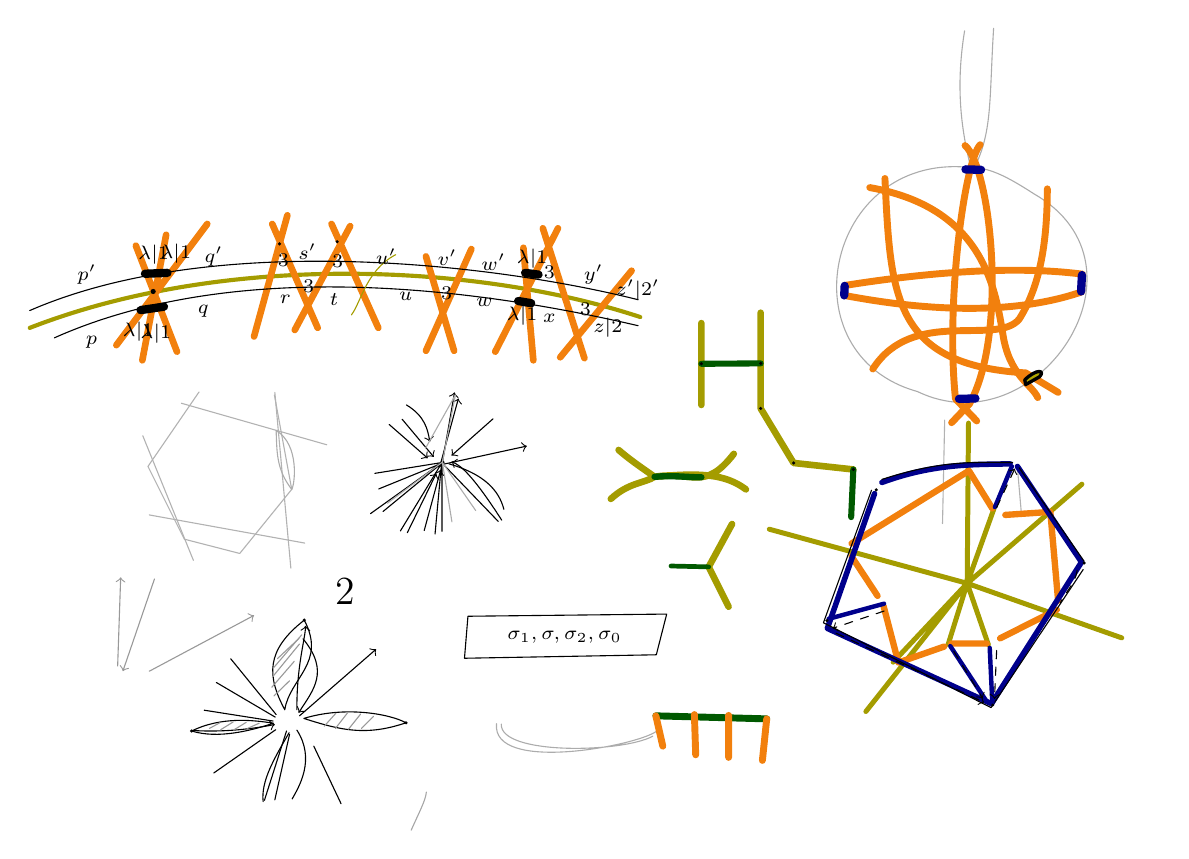
\begin{tikzpicture}[x=.055mm,y=-.055mm,line cap=round,line join=round,every node/.style={font=\scriptsize}]
% E03: upper strip.
\draw[olive!80!yellow,line width=1.5pt] (250,1025) .. controls (700,850) and (1280,875) .. (1660,1000);
\draw[orange!80!brown,line width=2.4pt] (450,1065)--(660,785) (495,835)--(590,1080) (510,1100)--(565,810);
\draw[orange!80!brown,line width=2.4pt] (768,1045)--(845,765) (810,785)--(915,1025) (862,1030)--(990,790) (947,785)--(1055,1025);
\draw[orange!80!brown,line width=2.4pt] (1165,860)--(1230,1078) (1165,1078)--(1270,843);
\draw[orange!80!brown,line width=2.4pt] (1325,1080)--(1470,795) (1390,840)--(1413,1100) (1435,795)--(1531,1095) (1475,1093)--(1640,893);
\draw (250,985) .. controls (675,800) and (1325,877) .. (1655,960);
\draw (307,1048) .. controls (730,859) and (1290,935) .. (1655,1020);
\draw[line width=3pt] (516,900)--(568,898) (506,984)--(560,976) (1394,898)--(1425,902) (1378,963)--(1408,968);
\fill (535,941) circle (6); \fill (827,831) circle (4); \fill (960,826) circle (4);
\draw[olive!80!yellow] (993,995) .. controls (1015,966) and (1027,892) .. (1095,856);
\node at (382,902) {$p'$}; \node at (393,1058) {$p$};
\node at (536,857) {$\unsure{\lambda|1}$}; \node at (587,854) {$\unsure{\lambda|1}$};
\node at (500,1034) {$\unsure{\lambda|1}$}; \node at (541,1038) {$\unsure{\lambda|1}$};
\node at (675,861) {$q'$}; \node at (651,987) {$q$};
\node at (840,960) {$r$}; \node at (836,870) {$\unsure{3}$};
\node at (891,849) {$s'$}; \node at (894,929) {$\unsure{3}$};
\node at (953,960) {$t$}; \node at (961,871) {$\unsure{3}$};
\node at (1073,860) {$u'$}; \node at (1118,952) {$u$};
\node at (1214,863) {$v'$}; \node at (1213,944) {$\unsure{3}$};
\node at (1321,873) {$w'$}; \node at (1300,967) {$w$};
\node at (1410,866) {$\unsure{\lambda|1}$}; \node at (1387,997) {$\unsure{\lambda|1}$};
\node at (1450,896) {$\unsure{3}$}; \node at (1450,1003) {$x$};
\node at (1552,902) {$y'$}; \node at (1533,982) {$\unsure{3}$};
\node at (1654,938) {$\unsure{z'|2'}$}; \node at (1585,1024) {$\unsure{z|2}$};
% E04: upper-right coloured arrangement, including pale pencil boundary.
\draw[gray!65] (2409,339) .. controls (2390,455) and (2398,552) .. (2421,645);
\draw[gray!65] (2476,333) .. controls (2466,495) and (2473,567) .. (2435,648);
\draw[gray!65] (2415,654) .. controls (2087,625) and (1994,1087) .. (2300,1172) .. controls (2576,1305) and (2860,883) .. (2570,716) .. controls (2505,674) and (2464,653) .. (2415,654);
\draw[orange!80!brown,line width=2.5pt] (2410,604) .. controls (2470,655) and (2510,1040) .. (2420,1201)--(2379,1244);
\draw[orange!80!brown,line width=2.5pt] (2445,602) .. controls (2408,642) and (2365,969) .. (2388,1189)--(2437,1240);
\draw[orange!80!brown,line width=2.5pt] (2190,701) .. controls (2450,747) and (2479,930) .. (2497,1037) .. controls (2511,1135) and (2564,1155) .. (2578,1186);
\draw[orange!80!brown,line width=2.5pt] (2225,680) .. controls (2238,948) and (2242,1111) .. (2550,1129)--(2625,1174);
\draw[orange!80!brown,line width=2.5pt] (2197,1120) .. controls (2289,976) and (2482,1068) .. (2535,1005) .. controls (2574,943) and (2600,855) .. (2600,704);
\draw[orange!80!brown,line width=2.5pt] (2133,927) .. controls (2315,898) and (2520,880) .. (2681,901)--(2679,942) .. controls (2493,1006) and (2263,975) .. (2131,950)--cycle;
\draw[blue!55!black,line width=3pt] (2132,928)--(2131,950) (2680,903)--(2678,941) (2411,659)--(2447,660) (2396,1189)--(2434,1188);
\draw[line width=1.2pt,fill=olive!70!yellow] (2548,1145) .. controls (2576,1118) and (2596,1123) .. (2582,1138)--(2550,1156)--cycle;
% E05: pale polygon construction at left centre.
\draw[gray!60] (641,1173)--(523,1345)--(607,1513)--(735,1546)--(855,1398)--(815,1180);
\draw[gray!60] (511,1274)--(628,1562) (526,1457)--(885,1522) (600,1199)--(936,1295) (816,1174)--(853,1580);
\draw[gray!65] (819,1262) .. controls (874,1295) and (862,1388) .. (855,1398) .. controls (819,1351) and (821,1312) .. (819,1262);
% E06: radial arrows.
\fill (1203,1336) circle (5);
\draw[->] (1203,1336)--(1231,1174); \draw[->] (1200,1334)--(1240,1188);
\draw[->] (1205,1340)--(1398,1298);
\draw[->] (1320,1235)--(1224,1320);
\draw[->] (1120,1203).. controls (1163,1229) and (1169,1260)..(1174,1288);
\draw[->] (1110,1236)--(1183,1323); \draw[->] (1080,1248)--(1169,1326);
\draw[->] (1340,1469)..controls (1271,1362) and (1244,1342)..(1224,1334);
\draw[->] (1122,1498)--(1189,1361); \draw[->] (1161,1493)--(1199,1353);
\draw (1047,1361)--(1202,1336)--(1037,1454) (1056,1397)--(1201,1338)--(1106,1494) (1066,1449)--(1201,1338)--(1186,1501) (1202,1495)--(1202,1337)--(1332,1472) (1218,1339)..controls(1297,1362)and(1333,1398)..(1345,1444);
\draw[gray!65] (1164,1303)--(1233,1180)--(1203,1335)--(1076,1430) (1225,1473)--(1203,1336)--(1280,1447);
% E07: the three small green graphs and bent continuation.
\draw[olive!80!yellow,line width=2.4pt] (1801,1014)--(1801,1203) (1938,990)--(1938,1211)--(2014,1337)--(2152,1352);
\draw[green!35!black,line width=2.2pt] (1801,1108)--(1938,1107) (2152,1352)--(2147,1462);
\foreach \x/\y in {1801/1108,1938/1107,1938/1211,2014/1337,2152/1352}{\fill (\x,\y) circle (4);}
\draw[olive!80!yellow,line width=2.4pt] (1610,1307)..controls(1640,1333)and(1668,1351)..(1693,1369)..controls(1779,1354)and(1807,1405)..(1876,1316) (1592,1420)..controls(1633,1382)and(1669,1384)..(1693,1369)..controls(1797,1359)and(1856,1362)..(1904,1398);
\draw[green!35!black,line width=2.3pt] (1693,1369)..controls(1739,1365)and(1778,1371)..(1801,1370);
\draw[olive!80!yellow,line width=2.4pt] (1872,1478)--(1818,1577)--(1864,1669);
\draw[green!35!black,line width=1.7pt] (1731,1575)--(1818,1577);
% E08: lower-right polygon, coloured spokes and perimeter arrows.
\draw[olive!80!yellow,line width=1.8pt] (2418,1245)--(2415,1615)--(2181,1911) (1958,1490)--(2415,1615)--(2772,1741) (2244,1797)--(2415,1615)--(2680,1386) (2415,1615)--(2371,1756) (2415,1615)--(2464,1757) (2415,1615)--(2477,1442);
\draw[gray!60] (2363,1238)--(2358,1477) (2531,1348)--(2540,1452);
\draw[orange!80!brown,line width=2.3pt] (2148,1523)--(2419,1355)--(2473,1442) (2503,1457)--(2607,1450)--(2625,1655) (2622,1676)--(2491,1742) (2460,1754)--(2378,1754) (2362,1761)--(2256,1798)--(2222,1668) (2208,1644)--(2148,1553);
\draw[blue!55!black,line width=2pt] (2218,1382)..controls(2340,1337)and(2435,1341)..(2514,1339) (2531,1345)--(2679,1566)--(2471,1893)--(2092,1719)--(2201,1408);
\draw (2218,1375)..controls(2360,1329)and(2435,1336)..(2520,1336) (2535,1348)--(2685,1564) (2683,1583)--(2470,1902)--(2083,1706)--(2194,1400);
\draw[blue!55!black,line width=1.6pt] (2518,1345)--(2479,1439) (2095,1697)--(2223,1662) (2376,1760)--(2460,1888) (2467,1764)--(2473,1892);
\draw[->,dashed] (2483,1440)--(2525,1350); \draw[->,dashed] (2223,1679)--(2104,1719); \draw[->,dashed] (2112,1730)--(2454,1890);
\draw[->,dashed] (2384,1772)--(2451,1881); \draw[->,dashed] (2483,1770)--(2478,1882);
\draw[dashed] (2669,1585)..controls(2665,1614)and(2643,1634)..(2630,1660);
\foreach \x/\y in {2205/1399,2091/1701,2685/1568,2474/1896}{\fill (\x,\y) circle (4);}
% E09: lower-left separate pencil arrows.
\draw[->,gray!80] (453,1806)--(460,1601); \draw[->,gray!80] (538,1605)--(465,1818); \draw[->,gray!80] (526,1818)--(768,1689);
% E10: lower four-lobed drawing and its numeral.
\node[font=\Large] at (978,1635) {$2$};
\draw (884,1700)..controls(794,1770)and(798,1830)..(839,1907)..controls(850,1834)and(936,1799)..(884,1700);
\draw (624,1956)..controls(693,1922)and(767,1931)..(813,1938)..controls(762,1955)and(684,1975)..(624,1956);
\draw (883,1927)..controls(977,1898)and(1080,1916)..(1119,1937)..controls(1028,1968)and(970,1955)..(883,1927);
\draw (849,1960)..controls(813,2022)and(784,2072)..(789,2119) (867,1954)..controls(911,2022)and(871,2086)..(856,2113);
\draw[->] (867,1907)..controls(866,1808)and(886,1744)..(887,1713);
\draw[->] (881,1743)..controls(944,1819)and(904,1862)..(871,1914);
\draw[->] (629,1955)..controls(701,1959)and(765,1951)..(816,1941);
\draw[->] (873,1921)--(1050,1767);
\draw (714,1789)--(819,1918) (681,1844)--(817,1924) (653,1908)--(812,1933) (675,2053)--(818,1953) (906,1991)--(969,2124) (792,2116)--(843,1956) (816,2115)--(850,1964);
\foreach \x/\y in {624/1956,884/1700,1119/1937}{\fill (\x,\y) circle (4);}
\foreach \x/\y/\u/\v in {814/1875/850/1840,809/1855/861/1795,810/1832/873/1755,814/1809/878/1734,822/1789/872/1742,665/1950/689/1937,691/1953/720/1935,722/1953/750/1936,753/1950/780/1938,930/1945/957/1915,956/1950/984/1914,986/1952/1014/1917,1016/1950/1044/1922}{\draw[gray!80] (\x,\y)--(\u,\v);}
\draw[gray!70] (1131,2185)..controls(1150,2142)and(1164,2117)..(1166,2097);
% E11: boxed symbols.
\draw (1262,1691)--(1721,1686)--(1697,1780)--(1254,1788)--cycle;
\node at (1485,1740) {$\sigma_1,\sigma,\sigma_2,\sigma_0$};
% E12: faint curve and bottom comb.
\draw[gray!65] (1328,1939)..controls(1316,2054)and(1649,1991)..(1697,1957) (1339,1940)..controls(1335,2012)and(1617,2007)..(1689,1968);
\draw[green!35!black,line width=2.5pt] (1696,1921)--(1952,1928);
\draw[orange!80!brown,line width=2.5pt] (1696,1921)--(1712,1991) (1785,1918)--(1788,2011) (1864,1920)--(1864,2017) (1952,1928)--(1942,2024);
\end{tikzpicture}}
\margin{\mspage{126}}

\scanpage{128}
\figure{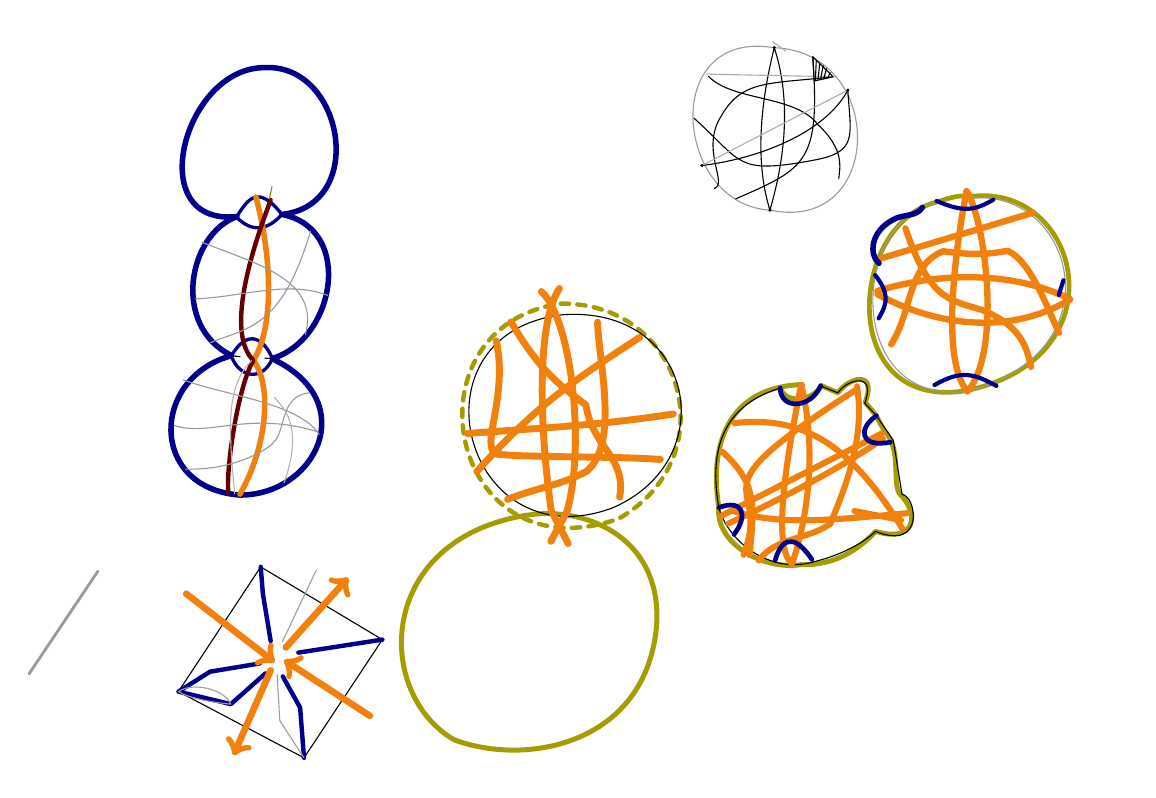
\begin{tikzpicture}[x=.055mm,y=-.055mm,line cap=round,line join=round]
% E01: three vertically joined outlines at left.
\draw[blue!55!black,line width=2pt] (705,547)..controls(485,570)and(582,201)..(770,203)..controls(951,194)and(1008,520)..(809,542)..controls(978,575)and(931,832)..(786,875)..controls(997,975)and(885,1192)..(711,1190)..controls(501,1174)and(505,919)..(693,868)..controls(553,800)and(592,588)..(705,547);
\draw[blue!55!black,line width=1.2pt] (704,548)..controls(730,508)and(752,470)..(809,542)..controls(775,580)and(739,584)..(704,548);
\draw[blue!55!black,line width=1.2pt] (692,869)..controls(732,801)and(769,832)..(787,875)..controls(764,928)and(711,920)..(692,869);
\draw[dashed] (693,869)--(787,875);
\draw[orange!80!brown,line width=2pt] (749,502)..controls(792,666)and(785,815)..(743,879)..controls(787,936)and(775,1078)..(712,1188);
\draw[red!40!black,line width=1.6pt] (783,509)..controls(729,651)and(683,819)..(743,879)..controls(709,936)and(680,1120)..(685,1184);
\draw[olive] (780,505)--(786,478);
\draw[gray!80] (624,606)..controls(734,652)and(900,688)..(863,820) (608,737)..controls(718,733)and(821,693)..(915,729) (644,838)..controls(730,803)and(808,806)..(875,581);
\draw[gray!80] (581,924)..controls(673,959)and(848,977)..(895,1050) (560,1029)..controls(638,1057)and(730,995)..(888,1043) (587,1130)..controls(691,1134)and(775,1088)..(791,1067)..controls(818,1041)and(804,961)..(872,954);
\draw[gray!60] (700,1187)..controls(685,1032)and(680,938)..(739,880) (814,1162)..controls(862,1027)and(809,986)..(792,965);
% E02: top right pencil arrangement, with hatched cap.
\draw[gray!80] (1946,157)..controls(1679,112)and(1716,520)..(1936,532)..controls(2201,588)and(2207,167)..(1946,157)--cycle;
\draw (1794,223)..controls(1849,281)and(1997,266)..(2047,335)..controls(2110,393)and(2097,437)..(2095,459);
\draw (1761,320)..controls(1875,423)and(1856,450)..(2036,417)..controls(2141,398)and(2122,361)..(2116,255);
\draw (1808,482)..controls(1840,470)and(1774,391)..(1824,314)..controls(1872,230)and(1936,241)..(2082,224);
\draw (2035,178)..controls(2052,421)and(2021,435)..(1857,506);
\draw (1946,157)..controls(1900,342)and(1913,458)..(1936,532)..controls(1977,392)and(1981,263)..(1946,157);
\draw (1779,429)..controls(1904,414)and(2061,357)..(2116,255);
\draw[gray!65] (1779,429)--(2116,255) (1789,218)--(2085,224) (1942,143)--(1973,165);
\draw (2035,178)--(2082,224)--(2038,234)--cycle;
\foreach \x/\y/\u/\v in {2043/187/2041/232,2051/193/2047/231,2059/198/2053/230,2067/205/2060/229,2075/214/2070/227}{\draw (\x,\y)--(\u,\v);}
\foreach \x/\y in {1946/157,1936/532,1779/429,2116/255}{\fill (\x,\y) circle (4);}
% E03: upper right coloured arrangement.
\draw[olive!80!yellow,line width=1.7pt] (2391,502)..controls(2647,458)and(2758,868)..(2394,948)..controls(2093,1003)and(2114,573)..(2315,515)..controls(2344,507)and(2375,494)..(2391,502);
\draw[gray!80] (2390,506)..controls(2634,469)and(2748,857)..(2394,950)..controls(2110,989)and(2119,561)..(2316,515);
\draw[orange!80!brown,line width=2.3pt] (2390,488)..controls(2434,555)and(2472,860)..(2392,951)..controls(2323,870)and(2374,571)..(2390,488);
\draw[orange!80!brown,line width=2.3pt] (2191,644)--(2544,538) (2184,719)..controls(2329,674)and(2500,673)..(2630,738)..controls(2482,827)and(2307,794)..(2184,726);
\draw[orange!80!brown,line width=2.3pt] (2249,574)..controls(2304,737)and(2347,739)..(2424,762)..controls(2519,800)and(2529,851)..(2539,894);
\draw[orange!80!brown,line width=2.3pt] (2216,842)..controls(2265,766)and(2253,660)..(2336,627)..controls(2401,636)and(2436,635)..(2485,626)..controls(2542,652)and(2580,770)..(2604,815);
\draw[blue!55!black,line width=1.5pt] (2321,511)..controls(2384,538)and(2409,533)..(2452,508) (2179,682)..controls(2210,722)and(2210,744)..(2187,782) (2614,694)--(2603,728) (2316,936)..controls(2379,900)and(2407,910)..(2459,938);
\draw[blue!55!black,line width=2pt] (2288,526)..controls(2275,548)and(2242,541)..(2221,554)..controls(2168,581)and(2164,635)..(2188,655);
% E04: central circular arrangement, dashed outer contour and lower empty loop.
\draw[olive!80!yellow,line width=1.8pt] (1373,1237)..controls(1027,1293)and(1021,1646)..(1206,1755)..controls(1379,1820)and(1658,1762)..(1675,1481)..controls(1681,1279)and(1499,1215)..(1373,1237);
\draw[olive!80!yellow,dashed,line width=1.6pt] (1453,748)..controls(1738,745)and(1837,1102)..(1586,1245)..controls(1192,1382)and(1082,802)..(1453,748);
\draw (1454,774)..controls(1760,749)and(1832,1108)..(1572,1220)..controls(1228,1346)and(1094,820)..(1454,774);
\draw[orange!80!brown,line width=2.5pt] (1408,720)..controls(1477,782)and(1511,1075)..(1467,1229)--(1430,1297) (1450,713)..controls(1394,795)and(1406,1052)..(1431,1226)--(1470,1302);
\draw[orange!80!brown,line width=2.5pt] (1338,790)..controls(1406,908)and(1461,944)..(1511,982)..controls(1526,1081)and(1605,1101)..(1589,1195) (1259,1136)..controls(1410,966)and(1518,904)..(1635,826);
\draw[orange!80!brown,line width=2.5pt] (1304,834)..controls(1333,967)and(1262,1085)..(1307,1096)..controls(1395,1104)and(1583,1100)..(1683,1108) (1237,1048)..controls(1437,1033)and(1532,1030)..(1713,1003);
\draw[orange!80!brown,line width=2.5pt] (1538,791)..controls(1540,881)and(1589,1070)..(1513,1135)..controls(1452,1168)and(1408,1170)..(1330,1200);
% E05: right lower scalloped outline and curves.
\draw[olive!80!yellow,line width=1.8pt] (2011,935)..controls(1833,940)and(1796,1083)..(1818,1218)..controls(1809,1300)and(1918,1364)..(2006,1351)..controls(2104,1354)and(2159,1296)..(2180,1274)..controls(2269,1301)and(2282,1239)..(2241,1193)..controls(2213,1174)and(2245,1086)..(2199,1040)--(2181,1006)--(2156,976)..controls(2185,897)and(2115,921)..(2093,954)--(2054,937)..controls(2046,965)and(1975,987)..(1960,943);
\draw (1960,943)..controls(1810,988)and(1799,1109)..(1818,1219)..controls(1837,1293)and(1934,1377)..(2042,1343)..controls(2117,1324)and(2162,1291)..(2180,1274)..controls(2293,1320)and(2276,1195)..(2241,1188)--(2221,1064)--(2182,1007)--(2155,978)..controls(2183,902)and(2112,924)..(2093,954)--(2053,938)..controls(2025,997)and(1956,986)..(1960,943);
\draw[orange!80!brown,line width=2.2pt] (2008,936)..controls(2045,1080)and(2024,1243)..(1987,1349)..controls(1935,1307)and(1985,1052)..(2008,936) (2137,939)..controls(2159,1071)and(2097,1200)..(2076,1256)..controls(2019,1296)and(1953,1285)..(1910,1341);
\draw[orange!80!brown,line width=2.2pt] (1854,1024)..controls(2012,1006)and(2121,1072)..(2241,1266) (1826,1090)..controls(1908,1165)and(1900,1216)..(1889,1329) (1875,1328)..controls(1946,1147)and(1736,1202)..(2135,947);
\draw[orange!80!brown,line width=2.2pt] (1822,1239)--(2196,1047) (1840,1256)..controls(1960,1200)and(2096,1130)..(2197,1060) (1852,1227)..controls(1953,1260)and(2071,1249)..(2253,1232) (2131,1227)--(2239,1248);
\draw[blue!55!black,line width=1.7pt] (1960,943)..controls(1959,992)and(2029,993)..(2053,938) (2182,1007)..controls(2140,1035)and(2141,1082)..(2214,1068) (1818,1219)..controls(1874,1198)and(1887,1237)..(1853,1281) (1948,1341)..controls(1968,1273)and(2003,1294)..(2033,1339);
% E06: bottom-left polygon and arrows; detached pencil stroke.
\draw[gray!80,line width=1pt] (225,1603)--(384,1366);
\draw (570,1644)--(760,1356)--(1041,1524)--(860,1797)--cycle;
\draw[blue!55!black,line width=1.6pt] (760,1356)--(765,1418)--(783,1527) (847,1554)--(1041,1524) (811,1609)--(851,1681)--(860,1797) (570,1644)--(643,1598)--(758,1579) (570,1644)--(691,1673)--(771,1602);
\draw[gray!75] (860,1797)--(804,1711)--(798,1605) (570,1644)..controls(605,1620)and(678,1640)..(691,1673)..controls(637,1668)and(590,1657)..(570,1644) (888,1364)--(810,1529);
\draw[orange!80!brown,->,line width=2.4pt] (588,1418)--(792,1576);
\draw[orange!80!brown,->,line width=2.4pt] (1012,1700)--(814,1571);
\draw[orange!80!brown,->,line width=2.4pt] (783,1595)--(697,1791);
\draw[orange!80!brown,->,line width=2.4pt] (818,1542)--(962,1381);
\end{tikzpicture}}

% E07: inverted printed matter; lines retained in their own reading direction.
\begin{center}\rotatebox{180}{\begin{minipage}{.95\linewidth}\ttfamily\small
J E S 2\quad J O B\quad L O G\quad --\quad S Y S T E M\quad E 3 3 3\quad --\quad N O D E\quad E 3 3\par
15.05.17 J0344CNU\quad \$ J0344*CRAY2\quad STARTED - INIT 10 - CLASS Q - SYS E333\par
15.05.19 J0344CNU\quad DSN CISI.PROD.CSSBATCH.V1.\unsure{YY01|YYO1}\par
15.05.28 J0344CNU\quad CSS2060 - JOB QUEUED FOR TRANSFER\par
15.05.28 J0344CNU\quad SMF RECORD 153-1 (CLOSE) WRITTEN\par
15.05.29 J0344CNU\quad \$ J0344*CRAY2\quad ENDED\par
------ JES2 JOB STATISTICS ------\par
19 AUG 82 JOB EXECUTION DATE\par
14 CARDS READ\par
99 SYSOUT PRINT RECORDS\par
0 SYSOUT PUNCH RECORDS\par
0.20 MINUTES EXECUTION TI\unsure{ME}
\end{minipage}}\end{center}
\margin{\mspage{127}}

\scanpage{129}
\figure{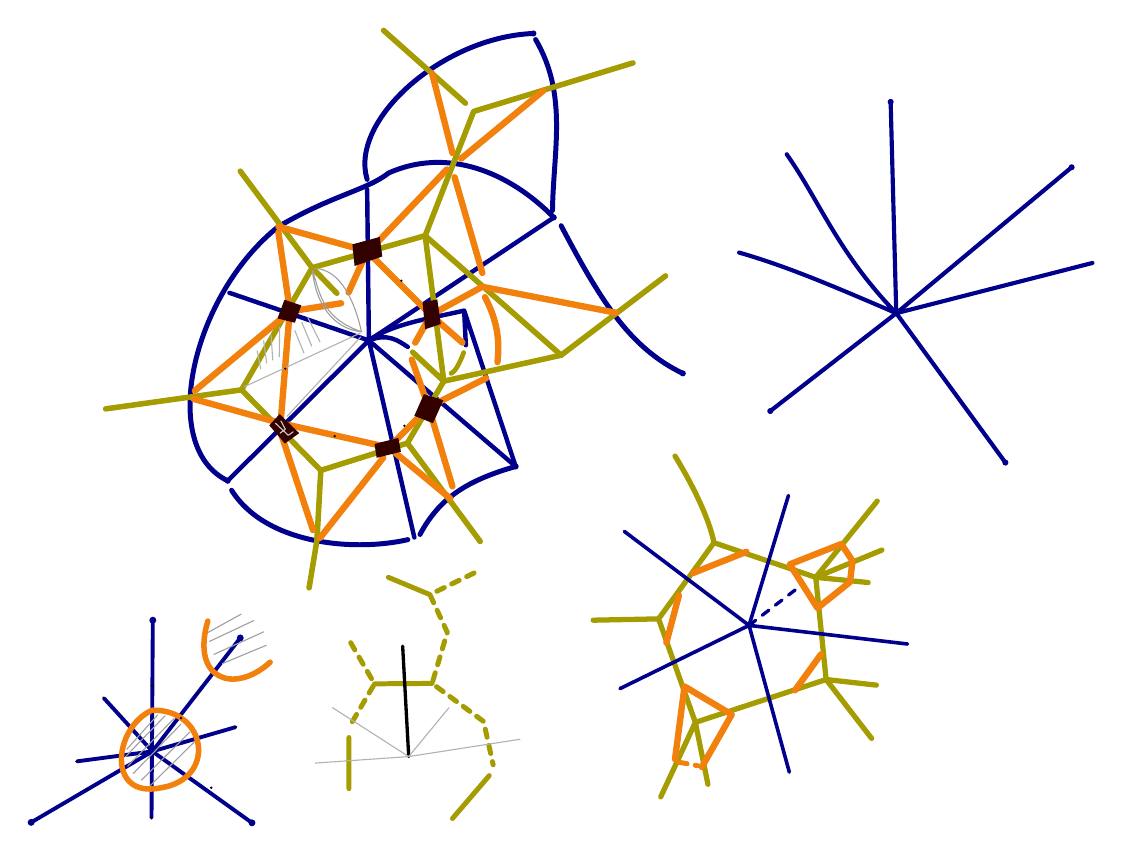
\begin{tikzpicture}[x=.055mm,y=-.055mm,line cap=round,line join=round]
% E01: large coloured construction at upper left.
\draw[blue!55!black,line width=1.8pt] (1370,191)..controls(1160,199)and(944,392)..(986,528) (1375,205)..controls(1450,333)and(1416,461)..(1414,600);
\draw[blue!55!black,line width=1.8pt] (664,1224)..controls(501,1146)and(582,795)..(781,637)..controls(906,564)and(985,553)..(1036,513)..controls(1169,454)and(1311,508)..(1417,616);
\draw[blue!55!black,line width=1.8pt] (1434,635)..controls(1524,806)and(1592,917)..(1715,976);
\draw[blue!55!black,line width=1.8pt] (673,1246)..controls(752,1372)and(958,1388)..(1080,1360) (1108,1348)..controls(1151,1268)and(1210,1225)..(1329,1191);
\draw[blue!55!black,line width=1.6pt] (986,551)--(990,900)--(1095,1355) (668,790)--(990,900)--(1329,1191) (664,1224)--(990,900)--(1417,616);
\draw[blue!55!black,line width=1.6pt] (990,900)..controls(1045,861)and(1133,849)..(1210,831)--(1329,1191) (1210,831)--(1214,911) (990,900)..controls(1035,882)and(1058,901)..(1080,915);
\draw[olive!80!yellow,line width=2pt] (1024,184)--(1213,352) (1600,259)--(1232,371)--(1120,658)--(859,732)--(696,1014)--(879,1200)--(1079,1137)--(1163,994)--(1434,934)--(1675,751);
\draw[olive!80!yellow,line width=2pt] (693,509)--(859,732)--(916,791) (1120,658)--(1163,994)--(1091,927) (1120,658)--(1434,934) (696,1014)--(382,1058) (879,1200)--(870,1362)--(852,1471) (1079,1137)--(1247,1364);
\draw[olive!80!yellow,line width=1.7pt] (1209,928)..controls(1198,957)and(1188,973)..(1180,976);
\draw[orange!80!brown,line width=2.3pt] (1136,283)--(1183,467) (1203,480)--(1393,323) (1170,505)--(1011,672) (1188,523)--(1252,744);
\draw[orange!80!brown,line width=2.3pt] (781,637)--(986,694)--(1133,841)--(1252,776)--(1561,836) (781,650)--(808,833)--(588,1016) (807,835)--(786,1091)--(585,1035) (786,1091)--(1036,1147)--(1128,1054)--(1261,987);
\draw[orange!80!brown,line width=2.3pt] (1258,800)..controls(1291,862)and(1291,909)..(1287,950) (1133,841)--(1206,905) (1133,841)--(1097,905) (1089,944)--(1128,1054)--(1183,1237);
\draw[orange!80!brown,line width=2.3pt] (1036,1147)--(1178,1265) (1023,1171)--(877,1356) (786,1112)--(861,1338) (808,833)--(926,814) (943,789)--(986,694);
\draw[gray!75] (859,733)..controls(866,816)and(908,873)..(973,880) (859,733)..controls(878,803)and(888,850)..(973,880) (859,733)..controls(928,732)and(959,818)..(973,880);
\draw[gray!60] (702,1007)--(970,883) (801,1075)--(971,892) (740,965)--(732,924) (754,952)--(747,901) (768,945)--(764,886) (783,938)--(784,869) (819,877)--(840,929) (835,858)--(858,913) (849,847)--(877,903);
\foreach \x/\y in {1370/191,1417/616,1715/976,1329/1191,664/1224}{\fill[blue!55!black] (\x,\y) circle (7);}
\foreach \x/\y in {1675/751,852/1471,1247/1364,1120/658,859/732,696/1014,879/1200,1163/994,1434/934}{\fill[olive!80!yellow] (\x,\y) circle (6);}
\fill[red!20!black] (952,678)--(1015,661)--(1021,706)--(957,728)--cycle;
\fill[red!20!black] (795,806)--(834,819)--(819,859)--(779,849)--cycle;
\fill[red!20!black] (1114,813)--(1148,805)--(1156,862)--(1120,874)--cycle;
\fill[red!20!black] (784,1070)--(829,1114)--(796,1138)--(760,1096)--cycle;
\draw[gray!40] (774,1091)--(804,1119)--(815,1111) (787,1086)--(797,1105)--(785,1114);
\fill[red!20!black] (1003,1139)--(1058,1125)--(1064,1157)--(1008,1171)--cycle;
\fill[red!20!black] (1117,1024)--(1162,1038)--(1138,1091)--(1095,1074)--cycle;
\foreach \x/\y in {1065/762,797/965,911/1121,1072/1097}{\fill (\x,\y) circle (3);}
% E02: upper-right fan.
\draw[blue!55!black,line width=1.5pt] (2195,349)--(2208,837)--(2460,1182) (1955,470)..controls(2032,580)and(2073,697)..(2208,837) (1845,697)..controls(1953,728)and(2057,772)..(2208,837)--(2661,721) (1917,1063)--(2208,837)--(2613,500);
\foreach \x/\y in {2195/349,2460/1182,1917/1063,2613/500}{\fill[blue!55!black] (\x,\y) circle (7);}
% E03: lower-right fan with green polygon and orange additions.
\draw[olive!80!yellow,line width=1.9pt] (1697,1167)..controls(1737,1232)and(1776,1311)..(1787,1367)--(1659,1543)--(1744,1782)--(2046,1683)--(2022,1447)--(1787,1367);
\draw[olive!80!yellow,line width=1.9pt] (1659,1543)--(1508,1546) (1744,1782)--(1664,1954) (1744,1782)--(1773,1925) (2046,1683)--(2151,1819) (2046,1683)--(2162,1696) (2022,1447)--(2143,1459) (2022,1447)--(2175,1384) (2022,1447)--(2164,1271);
\draw[orange!80!brown,line width=2.3pt] (1739,1437)--(1862,1388) (1706,1489)--(1677,1598) (1719,1699)--(1697,1867) (1719,1699)--(1828,1764)--(1759,1885);
\draw[orange!80!brown,dashed,line width=1.8pt] (1706,1874)--(1749,1882);
\draw[orange!80!brown,line width=2.3pt] (1974,1708)--(2034,1625) (1962,1417)--(2081,1370)--(2107,1409)--(2101,1458)--(2026,1518)--cycle;
\draw[blue!55!black,line width=1.3pt] (1580,1341)--(1868,1558)--(2234,1601) (1959,1258)--(1868,1558)--(1961,1897) (1570,1704)--(1868,1558);
\draw[blue!55!black,dashed,line width=1.2pt] (1868,1558)--(1976,1475);
% E04: bottom-left fan, orange circle, cap and pencil hatching.
\draw[blue!55!black,line width=1.4pt] (491,1546)--(488,2002) (210,2013)--(490,1849)--(693,1587) (378,1726)--(490,1849)--(720,2014) (316,1872)--(490,1849)--(682,1793);
\draw[orange!80!brown,line width=2pt] (489,1754)..controls(615,1750)and(641,1912)..(510,1933)..controls(383,1960)and(400,1794)..(489,1754);
\draw[orange!80!brown,line width=2pt] (618,1548)..controls(578,1684)and(680,1718)..(762,1643);
\foreach \x/\y/\u/\v in {431/1844/502/1765,428/1861/519/1767,433/1883/540/1773,446/1900/556/1786,465/1915/577/1804,485/1928/587/1827,619/1574/695/1532,622/1595/724/1547,632/1625/747/1573,652/1646/753/1604}{\draw[gray!75] (\x,\y)--(\u,\v);}
\foreach \x/\y in {491/1546,210/2013,693/1587,720/2014}{\fill[blue!55!black] (\x,\y) circle (8);}
\foreach \x/\y in {488/2002,378/1726,682/1793,316/1872,340/1936,593/1716,556/1772,626/1933,489/1697}{\fill (\x,\y) circle (3);}
% E05: lower central green dashed construction, dark and pale rays.
\draw[olive!80!yellow,line width=1.8pt] (1035,1447)--(1131,1487) (1003,1693)--(1136,1692) (944,1817)--(944,1935) (1183,2004)--(1268,1905);
\draw[olive!80!yellow,dashed,line width=1.8pt] (1233,1437)--(1131,1487)--(1171,1574)--(1136,1692)--(1255,1780)--(1277,1880) (948,1598)--(1003,1693)--(945,1792);
\draw[line width=1.2pt] (1068,1606)--(1082,1861);
\draw[gray!60] (866,1876)--(1082,1861)--(1339,1821) (906,1748)--(1082,1861)--(1175,1748);
\end{tikzpicture}}

% E06: faint reverse-side printed matter visible through this sheet.
\begin{center}\scalebox{1}[-1]{\begin{minipage}{.95\linewidth}\ttfamily\small\color{gray}
\unsure{J E S 2\quad J O B\quad L O G\quad --\quad S Y S T E M\quad E 3 3 3\quad --\quad N O D E\quad E 3 3}\par
\unsure{15.05.17 J0344CNU\quad \$ J0344*CRAY2\quad STARTED - INIT 10 - CLASS Q - SYS E333}\par
\unsure{15.05.19 J0344CNU\quad DSN CISI.PROD.CSSBATCH.V1.YY01}\par
\unsure{15.05.28 J0344CNU\quad CSS2060 - JOB QUEUED FOR TRANSFER}\par
\unsure{15.05.28 J0344CNU\quad SMF RECORD 153-1 (CLOSE) WRITTEN}\par
\unsure{15.05.29 J0344CNU\quad \$ J0344*CRAY2\quad ENDED}\par
\unsure{------ JES2 JOB STATISTICS ------}\par
\unsure{19 AUG 82 JOB EXECUTION DATE}\par
\unsure{14 CARDS READ}\par
\unsure{99 SYSOUT PRINT RECORDS}\par
\unsure{0 SYSOUT PUNCH RECORDS}\par
\unsure{0.20 MINUTES EXECUTION TIME}
\end{minipage}}\end{center}
\margin{\mspage{128}}

\scanpage{130}
\figure{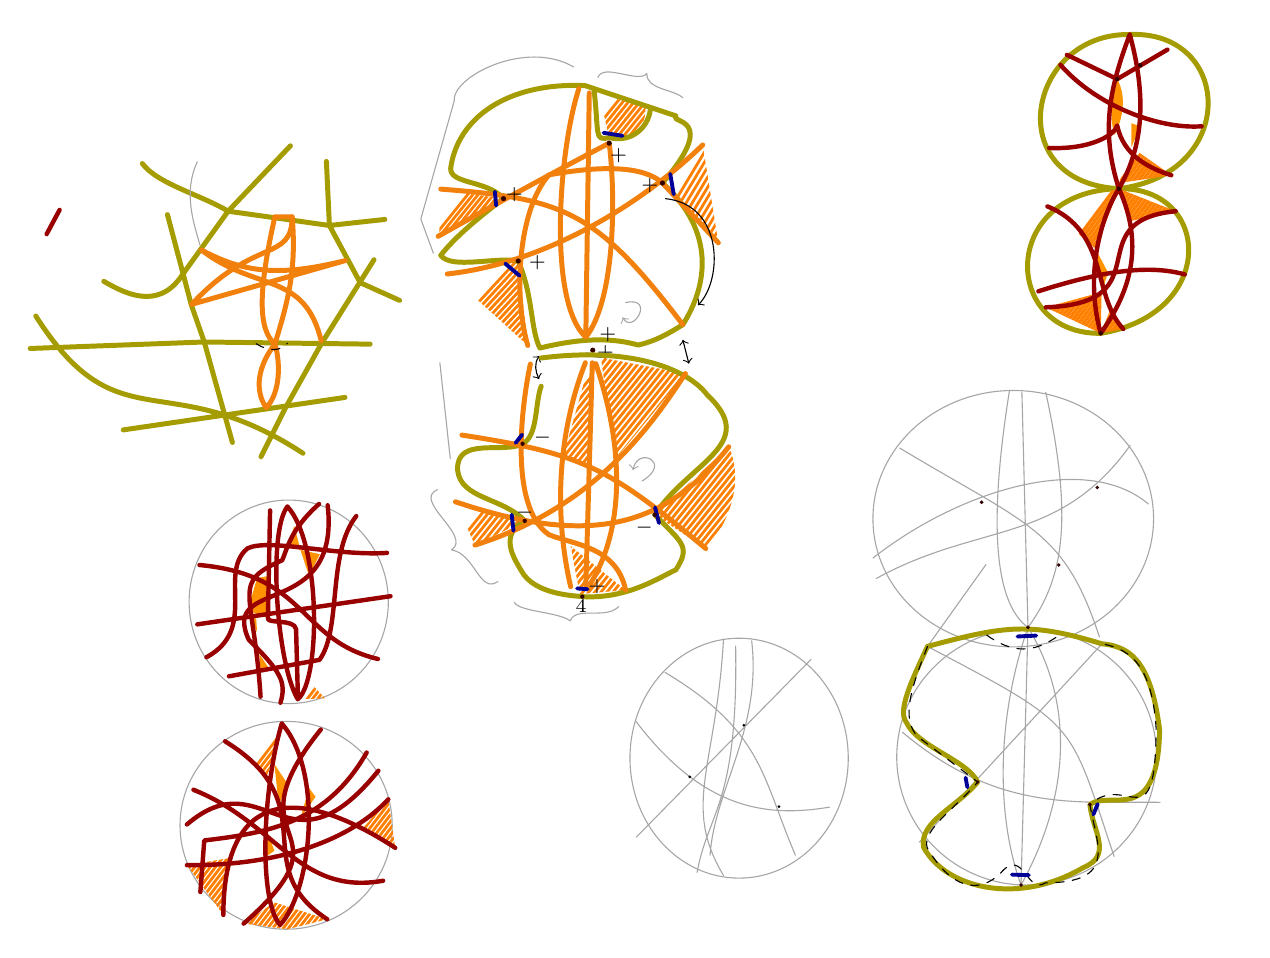
\begin{tikzpicture}[x=.55cm,y=-.55cm,line cap=round,line join=round,g/.style={olive!80!yellow,line width=1.8pt},r/.style={orange!80!brown,line width=1.8pt},w/.style={red!60!black,line width=1.6pt},p/.style={gray!70,thin},b/.style={blue!60!black,line width=1.4pt},every node/.style={font=\scriptsize}]
% E01: upper-left green graph and orange curves.
\draw[g] (3.35,3.68)..controls(3.7,4.15)and(4.7,4.4)..(5.33,4.78)--(6.77,3.27) (5.33,4.78)--(4.26,6.27)..controls(3.7,7.1)and(2.9,6.65)..(2.46,6.4) (3.93,4.86)--(4.48,6.94)--(4.78,7.8)--(5.43,10.12);
\draw[g] (5.33,4.78)--(7.67,5.11)--(8.95,4.97) (7.6,3.63)--(7.67,5.11)--(8.38,6.43)--(9.29,6.84) (8.7,5.9)--(7.49,7.83)--(6.65,9.33)--(6.09,10.45);
\draw[g] (.76,7.95)--(4.78,7.8)--(8.61,7.85) (.89,7.2)..controls(2.8,10.2)and(3.9,8.3)..(7.06,10.37) (2.91,9.83)--(8.03,9.08);
\draw[r] (4.72,5.68)..controls(5.7,6.2)and(6.5,6.3)..(8.04,5.92) (4.49,6.93)--(8.04,5.92) (4.49,6.93)..controls(5.95,5.36)and(6.8,5.96)..(6.81,4.91);
\draw[r] (6.41,4.91)..controls(6.02,6.65)and(6.02,7.5)..(6.41,7.85)..controls(6.73,6.81)and(6.91,6.1)..(6.81,4.91) (6.41,4.91)--(6.81,4.91) (6.41,7.85)..controls(6.02,8.35)and(5.93,8.91)..(6.21,9.32)..controls(6.6,8.9)and(6.5,8.1)..(6.41,7.85) (4.72,5.68)..controls(6,6.66)and(7.08,6.16)..(7.48,7.77);
\draw[p] (4.62,3.64)..controls(4.28,4.36)and(4.55,5.09)..(4.68,5.56);
\draw[w] (1.14,5.31)--(1.44,4.75);
\draw[dashed] (5.98,7.84)..controls(6.27,8.03)and(6.56,8.01)..(6.7,7.83);
% E02: central two-coloured arrangements, hatched boundary regions.
\begin{scope}
\clip (13.9,2.08)--(14.97,2.36)..controls(14.98,2.97)and(14.63,3.06)..(14.13,3.08)--cycle;
\foreach \k in {0,.13,...,2}{\draw[orange,line width=1pt] (13.4+\k,3.4)--(14.6+\k,1.9);}
\end{scope}
\begin{scope}
\clip (10.2,4.28)--(11.69,4.49)--(10.21,5.38)--cycle;
\foreach \k in {0,.12,...,2}{\draw[orange,line width=1pt] (9.9+\k,5.6)--(11.1+\k,4.1);}
\end{scope}
\begin{scope}
\clip (10.4,6.2)--(12.03,5.93)--(12.25,7.88)--cycle;
\foreach \k in {0,.14,...,3}{\draw[orange,line width=1pt] (9.9+\k,8.2)--(12.2+\k,5.7);}
\end{scope}
\begin{scope}
\clip (15.36,4.13)--(16.29,3.25)--(16.65,5.51)--cycle;
\foreach \k in {0,.14,...,3}{\draw[orange,line width=1pt] (14.9+\k,5.8)--(16.4+\k,3.3);}
\end{scope}
\draw[g] (13.57,1.88)..controls(11.75,1.8)and(10.62,2.65)..(10.47,3.79)..controls(10.45,4.16)and(11.32,4.06)..(11.69,4.49)..controls(11.16,4.89)and(10.57,5.37)..(10.24,5.8)..controls(10.48,6.13)and(11.51,5.83)..(12.03,5.93)..controls(12.38,6.75)and(12.31,7.51)..(12.53,7.94)..controls(13.6,7.68)and(14.25,7.72)..(14.8,7.87)..controls(15.2,7.78)and(15.51,7.6)..(15.83,7.4)..controls(16.4,6.5)and(16.6,5.26)..(15.36,4.13)..controls(16.7,2.57)and(15.5,2.76)..(15.67,2.58)--(13.57,1.88);
\draw[g] (13.78,1.97)..controls(13.9,3.04)and(13.78,3.16)..(14.13,3.08)..controls(14.64,3.21)and(15.03,2.85)..(15.08,2.44);
\draw[r] (13.43,1.95)..controls(12.97,3.35)and(12.7,6.86)..(13.59,7.69)..controls(14.26,6.83)and(14.29,4.5)..(14.13,3.21) (13.67,2.05)--(13.59,7.69);
\draw[r] (10.24,4.27)..controls(13.09,4.49)and(13.83,4.77)..(15.83,7.4) (10.18,5.36)..controls(11.75,4.48)and(13.28,3.65)..(14.13,3.21) (10.39,6.23)..controls(12.99,5.94)and(15.22,4.29)..(16.29,3.25);
\draw[r] (12.25,7.88)..controls(11.91,6.72)and(12.03,4.74)..(12.74,3.94)..controls(13.7,3.77)and(14.85,3.67)..(15.36,4.13)--(16.65,5.51);
\draw[p] (13.31,1.45)..controls(12.2,.8)and(10.49,1.68)..(10.55,2.24)--(9.78,4.96)--(10.07,5.75) (13.87,1.69)..controls(14.0,1.35)and(14.81,1.84)..(15.0,1.6)..controls(14.98,1.97)and(15.61,1.96)..(15.83,2.16) (10.22,8.28)--(10.46,10.49);
\draw[->] (15.43,4.49)..controls(16.78,4.63)and(16.75,6.37)..(16.18,6.95);
\draw[p,->] (14.51,6.89)..controls(15.2,6.74)and(14.68,7.64)..(14.44,7.23);
\draw[<->] (15.83,7.75)--(15.97,8.3);
\draw[<->] (12.52,8.12)..controls(12.39,8.3)and(12.43,8.48)..(12.51,8.66);
\foreach \x/\y in {14.35/3.5,11.94/4.39,15.07/4.2,12.47/5.97,14.1/7.62,14.04/8.05}{\node at (\x,\y) {$+$};}
\foreach \x/\y in {14.13/3.21,11.69/4.49,15.36/4.13,12.03/5.93,13.75/7.99}{\fill[red!20!black] (\x,\y) circle (.06);}
\draw[b] (14.0,2.97)--(14.44,3.04) (11.49,4.33)--(11.52,4.65) (15.54,3.92)--(15.62,4.39) (11.73,5.99)--(12.06,6.27) (13.59,8.09)--(13.98,8.12);
\begin{scope}
\clip (12.31,8.31)--(12.13,10.15)--(10.72,9.95)--cycle (13.7,8.2)--(13.07,10.44)--(13.71,10.67)--cycle (13.94,8.16)--(15.89,8.53)--(14.26,10.52)--cycle (15.18,11.79)--(16.89,10.22)..controls(17.32,11.16)and(16.72,12.23)..(16.36,12.57)--cycle (10.58,11.49)--(12.18,11.93)--(11.03,12.49)--cycle (13.24,12.51)--(14.51,13.53)--(13.45,13.62)--cycle;
\foreach \k in {0,.14,...,8}{\draw[orange,line width=1pt] (9.4+\k,14)--(14.6+\k,7.5);}
\end{scope}
\draw[g] (12.56,8.82)..controls(12.41,9.22)and(12.49,9.97)..(12.13,10.15)..controls(11.7,10.39)and(10.59,9.97)..(10.63,10.76)..controls(10.7,11.43)and(11.68,11.39)..(12.18,11.93)..controls(11.56,12.26)and(11.95,12.82)..(12.1,13.08)..controls(12.4,13.65)and(13.39,13.66)..(13.51,13.68)..controls(14.52,13.74)and(15.25,13.26)..(15.67,13.06)..controls(16.03,12.51)and(15.8,12.43)..(15.18,11.79)..controls(15.99,10.57)and(17.61,10.16)..(16.4,9.03)..controls(15.89,8.35)and(14.47,7.92)..(12.56,8.17);
\draw[r] (12.31,8.31)..controls(12.13,9.15)and(11.78,11.59)..(12.74,12.25)..controls(13.3,12.48)and(14.3,12.52)..(14.51,13.53) (13.58,8.28)..controls(13.06,9.6)and(12.78,11.43)..(13.24,13.45) (13.82,8.3)..controls(14.42,10.07)and(14.57,12.08)..(13.62,13.5) (13.74,8.28)--(13.59,13.44);
\draw[r] (10.73,9.95)..controls(13.53,10.38)and(14.12,10.7)..(16.36,12.57) (11.03,12.49)..controls(13.8,11.62)and(15.09,9.74)..(15.89,8.53) (10.58,11.49)..controls(13.59,12.5)and(15.36,12.16)..(16.89,10.22);
\draw[p,->] (14.89,11.01)..controls(15.6,10.58)and(14.79,10.2)..(14.68,10.76);
\draw[p] (10.17,11.21)..controls(9.56,11.45)and(10.98,12.28)..(10.49,12.6)..controls(11.03,12.69)and(11.14,13.63)..(11.56,13.33) (11.94,13.81)..controls(12.04,14.03)and(12.96,14.03)..(13.23,14.24)..controls(13.36,13.89)and(14.05,14.22)..(14.35,13.91);
\draw[b] (12.12,9.94)--(11.97,10.13) (11.88,11.79)--(11.92,12.16) (15.19,11.62)--(15.28,11.98) (13.39,13.49)--(13.63,13.51);
\foreach \x/\y in {12.59/10.02,12.18/11.73,14.94/12.08}{\node at (\x,\y) {$-$};}
\node at (13.85,13.45) {$+$}; \node at (13.48,13.91) {$\unsure{4}$};
\foreach \x/\y in {12.13/10.15,12.18/11.93,15.18/11.79,13.51/13.68}{\fill[red!20!black] (\x,\y) circle (.05);}
% E03: two small upper-right circles.
\fill[orange!85!yellow] (25.86,1.73)..controls(25.72,2.15)and(25.68,2.65)..(25.8,3.02)..controls(26.01,2.61)and(26.07,2.1)..(25.86,1.73);
\fill[orange!85!yellow] (26.19,2.75)--(26.39,2.82)--(26.19,3.3)--cycle (25.36,5.65)--(25.65,6.2)--(25.5,6.65)--cycle;

\draw[g] (26.15,.7)..controls(28.53,.6)and(28.68,3.91)..(25.9,4.26)..controls(23.15,4.12)and(23.77,.67)..(26.15,.7);
\draw[g] (25.9,4.26)..controls(28.05,4.23)and(28.18,7.15)..(25.48,7.6)..controls(23.19,7.63)and(23.13,4.32)..(25.9,4.26);
\begin{scope}
\clip (24.7,1.17)--(25.86,1.73)--(26.09,.77)--cycle (26.29,.78)--(26.39,1.41)--(27.02,1.05)--cycle (24.29,3.32)--(25.8,3.02)--(25.88,4.13)--cycle (25.9,4.13)--(26.19,3.3)--(27.11,3.95)--cycle (24.25,4.67)--(25.9,4.26)--(25.36,5.65)--cycle (25.9,4.26)--(26.16,5.01)--(27.21,4.78)--cycle (24.21,7.0)--(25.5,6.65)--(25.48,7.6)--cycle (25.48,7.6)--(25.72,7.0)--(26.0,7.5)--cycle;
\foreach \k in {0,.1,...,5}{\draw[orange,line width=1.2pt] (23+\k,8)--(29+\k,0);}
\end{scope}
\draw[w] (26.15,.7)..controls(26.59,2.3)and(26.4,3.39)..(25.9,4.26)..controls(25.46,2.9)and(25.7,1.9)..(26.15,.7) (24.7,1.17)--(25.86,1.73)--(27.02,1.05) (24.55,1.4)..controls(25.38,2.35)and(26.82,2.89)..(27.81,2.82) (24.29,3.32)..controls(25.25,3.36)and(25.81,3.02)..(25.86,2.8)..controls(26.0,3.49)and(26.59,3.79)..(27.11,3.95);
\draw[w] (25.9,4.26)..controls(26.54,5.67)and(26.08,6.75)..(25.48,7.6)..controls(25.07,6.12)and(25.56,4.78)..(25.9,4.26) (24.25,4.67)..controls(25.67,5.25)and(25.28,6.73)..(26.0,7.5) (24.21,7.0)..controls(26.95,6.9)and(24.9,5.01)..(27.21,4.78) (24.04,6.63)..controls(25.6,6.13)and(26.63,6.02)..(27.42,6.24);
\foreach \x/\y in {25.86/1.73,26.39/1.41,25.9/4.26,25.48/7.6}{\fill[red!20!black] (\x,\y) circle (.05);}
% E04 and E05: two lower-left red arrangements.
\fill[orange!85!yellow] (6.86,12.05)--(7.0,12.6)--(6.7,12.5)--cycle (7.0,12.6)--(7.45,12.7)--(7.2,13.2)--cycle (6.0,13.25)--(6.28,13.2)--(6.25,14.17)--(5.78,14.0)--cycle (5.78,14.0)--(6.0,14.5)--(5.98,14.2)--cycle (6.05,15.0)--(6.25,15.3)--(6.08,15.4)--cycle (6.4,17.55)--(6.7,18.0)--(6.5,18.5)--cycle (7.2,18.1)--(7.35,18.3)--(7.0,18.8)--cycle (6.2,19.0)--(6.4,19.55)--(6.18,19.7)--cycle;

\draw[p] (6.73,13.80) ellipse (2.3 and 2.35);
\draw[p] (6.67,18.96) ellipse (2.45 and 2.4);
\begin{scope}
\clip (7.92,12.68)--(8.29,11.82)--(9.0,12.67)--cycle (4.62,14.32)--(5.46,14.22)--(4.83,15.08)--cycle (5.35,15.52)--(6.08,15.38)--(6.08,15.99)--cycle (6.91,16.05)--(7.16,15.6)--(7.57,16.03)--cycle (5.26,17.02)--(6.57,16.61)--(6.24,17.83)--cycle (4.53,18.14)--(4.38,18.94)--(5.16,18.46)--cycle (8.44,19.03)--(9.03,18.36)--(9.19,19.48)--cycle (4.38,19.88)--(5.34,19.72)--(5.22,21.03)--cycle (5.69,21.23)--(6.4,20.74)--(7.62,21.13)--(6.7,21.36)--cycle;
\foreach \k in {0,.12,...,6}{\draw[orange,line width=1pt] (3+\k,21.5)--(11+\k,11);}
\end{scope}
\draw[w] (6.3,11.69)--(6.25,14.17)..controls(6.2,14.32)and(6.86,14.18)..(6.9,14.43)--(6.94,15.91) (6.7,11.6)..controls(7.48,12.45)and(7.47,15.61)..(6.94,16.05)..controls(6.45,15.23)and(6.24,12.19)..(6.7,11.6) (7.63,11.57)..controls(7.93,14.26)and(5.12,13.19)..(5.81,14.68)..controls(6.56,15.42)and(6.68,15.66)..(6.54,16.13);
\draw[w] (7.43,11.54)..controls(6.77,12.13)and(6.7,12.56)..(6.58,12.84)..controls(5.39,13.37)and(5.92,13.49)..(6.08,15.99) (8.29,11.82)..controls(7.61,12.69)and(7.96,14.43)..(7.44,15.14)--(5.35,15.52) (4.62,14.32)--(9.08,13.67) (4.83,15.08)..controls(6.03,14.43)and(5.09,13.16)..(5.77,12.57)..controls(6.25,12.32)and(7.82,12.75)..(9.0,12.67) (4.67,12.95)..controls(7.18,13.18)and(6.95,14.68)..(8.79,15.12);
\draw[w] (6.57,16.61)..controls(6.13,18.1)and(6.02,20.67)..(6.53,21.26)..controls(7.24,20.5)and(7.56,17.76)..(6.57,16.61) (7.47,16.75)..controls(5.25,19.5)and(8.33,18.9)..(5.69,21.23) (5.26,17.02)..controls(7.63,18.48)and(5.72,19.89)..(7.62,21.13) (4.53,18.14)..controls(6.45,18.9)and(6.96,20.59)..(8.91,20.24) (4.38,18.94)..controls(6.18,17.4)and(6.7,20.3)..(8.8,17.7) (4.38,19.88)..controls(6.63,19.9)and(8.22,19.24)..(9.03,18.36) (4.69,20.5)--(4.78,19.31)..controls(6.3,19.13)and(7.61,18.89)..(8.53,17.28) (5.22,21.03)..controls(5.23,18.14)and(6.91,18.0)..(9.19,19.48);
% E06: lower-centre pencil circle.
\draw[p] (17.13,17.41) ellipse (2.52 and 2.77);
\draw[p] (16.77,14.66)..controls(16.6,17.64)and(15.8,18.49)..(16.77,20.12) (17.05,14.82)..controls(17.11,18.51)and(16.41,18.64)..(16.16,20.05) (17.42,14.7)..controls(17.66,16.74)and(16.56,18.13)..(16.46,19.65) (15.42,15.43)..controls(17.68,16.78)and(17.66,17.86)..(18.43,19.65) (14.74,16.55)..controls(16.28,18.58)and(17.74,18.79)..(19.22,18.54) (14.76,19.23)--(18.79,15.13);
\foreach \x/\y in {15.99/17.84,17.24/16.65,18.05/18.53}{\fill (\x,\y) circle (.035);}
% E07: right-hand pencil pair and irregular green boundary.
\draw[p] (23.46,11.88) ellipse (3.24 and 2.96);
\draw[p] (23.77,17.38) ellipse (3.0 and 2.96);
\draw[p] (23.37,8.94)..controls(22.94,11.64)and(22.94,13.77)..(23.8,14.39)..controls(24.66,13.23)and(24.83,11.8)..(24.21,8.96) (23.66,8.96)--(23.8,14.39) (20.84,10.25)..controls(23.81,12.04)and(24.63,12.11)..(25.45,14.61) (20.22,12.79)..controls(22.15,11.27)and(25.1,10.3)..(26.58,11.54) (20.3,13.26)..controls(22.68,11.95)and(24.5,12.5)..(26.16,10.19) (21.48,14.83)--(22.83,12.94);
\draw[p] (21.48,14.83)..controls(25.03,16.7)and(24.73,16.54)..(25.79,19.68) (20.9,16.81)..controls(23.14,18.69)and(24.96,18.4)..(26.85,18.43) (23.8,14.39)..controls(23.06,16.53)and(23.07,18.77)..(23.64,20.34)..controls(24.79,18.25)and(24.86,16.12)..(23.8,14.39) (23.8,14.39)--(23.64,20.34) (21.29,19.35)--(25.51,14.77);
\draw[g] (21.48,14.83)..controls(21.11,15.63)and(20.78,16.32)..(20.99,16.58)..controls(21.25,17.15)and(22.39,17.45)..(22.64,17.96)..controls(22.15,18.55)and(21.28,18.88)..(21.39,19.47)..controls(21.93,20.45)and(23.61,20.8)..(25.07,19.94)..controls(25.78,19.65)and(25.29,19.1)..(25.23,18.48)..controls(25.72,18.13)and(26.8,19.01)..(26.84,16.76)..controls(26.66,15.35)and(26.27,14.83)..(25.51,14.77)..controls(23.85,14.27)and(23.3,14.34)..(21.48,14.83);
\draw[dashed] (21.48,14.83)..controls(21.11,15.78)and(20.86,16.48)..(21.25,16.91)--(22.64,17.96)..controls(22.15,18.55)and(21.35,19.06)..(21.47,19.47)..controls(22.0,20.4)and(22.65,20.59)..(23.18,20.05)..controls(23.69,19.46)and(23.78,20.58)..(24.2,20.29)..controls(25.88,20.28)and(25.39,19.43)..(25.23,18.48)..controls(26.09,17.7)and(26.74,19.4)..(26.76,16.73)..controls(26.67,15.38)and(26.25,14.9)..(25.51,14.77) (22.85,14.57)..controls(23.45,15.0)and(23.94,14.99)..(24.52,14.57);
\draw[b] (23.56,14.6)--(23.99,14.58) (22.36,17.86)--(22.4,18.08) (25.41,18.47)--(25.31,18.71) (23.43,20.1)--(23.82,20.11);
\foreach \x/\y in {22.73/11.5,25.4/11.16,24.51/12.95,23.8/14.39,22.64/17.96,25.23/18.48,23.64/20.34}{\fill[red!20!black] (\x,\y) circle (.045);}
\end{tikzpicture}}
\margin{\mspage{129}}

\scanpage{131}
% E01: printed listing.
{\ttfamily\small
\$HASP373 STARTED - INIT 1 - CLASS 1 - SYS E333\par
IEF236I ALLOC. FOR CRAY2\par
IEF142I CRAY2 - STEP WAS EXECUTED - COND CODE 0000\par
IEF373I STEP /\qquad / START 82228.1615\par
IEF374I STEP /\qquad / STOP 82228.1615 CPU 0MIN 00.02SEC SRB\quad 0MIN 00.00SEC VIRT\qquad 8K SYS\quad 164K\par
IEF375I JOB /CRAY2\quad / START 82228.1615\par
IEF376I JOB /CRAY2\quad / STOP 82228.1615 CPU\quad 0MIN 00.02SEC SRB\quad 0MIN 00.00SEC\par}

\figure{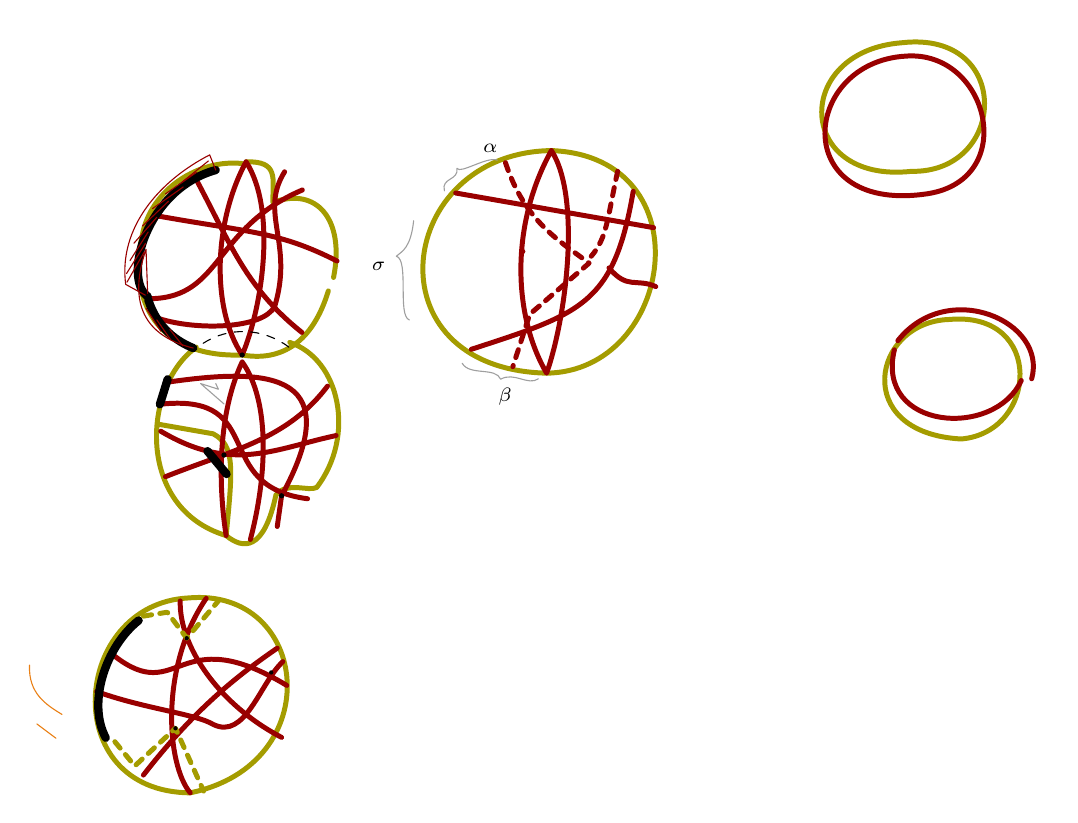
\begin{tikzpicture}[x=.55cm,y=-.55cm,line cap=round,line join=round,g/.style={olive!80!yellow,line width=1.8pt},r/.style={red!60!black,line width=1.8pt},p/.style={gray!75,thin},every node/.style={font=\scriptsize}]
% E02: joined arrangements at left, marked and overtraced boundary.
\draw[g] (7.88,5.32)..controls(8.65,5.3)and(8.49,5.71)..(8.5,6.26)..controls(9.5,5.88)and(10.17,6.64)..(9.9,7.99) (9.78,8.3)..controls(9.42,9.48)and(8.71,9.94)..(7.79,9.78)..controls(5.82,9.85)and(5.15,8.51)..(5.48,7.03)..controls(5.68,5.93)and(6.82,5.25)..(7.79,5.36);
\draw[g] (6.73,9.6)..controls(5.49,10.48)and(5.31,13.32)..(7.42,13.95)..controls(7.57,12.4)and(7.63,11.87)..(7.12,11.6)--(5.86,11.38) (7.42,13.95)..controls(7.81,14.27)and(8.29,14.32)..(8.57,13.01)..controls(8.84,12.69)and(9.31,12.94)..(9.51,12.84)..controls(10.42,11.65)and(10.05,9.88)..(8.89,9.49);
\draw[r] (7.88,5.32)..controls(8.6,6.44)and(8.25,8.7)..(7.79,9.78)..controls(7.07,8.7)and(7.13,6.71)..(7.88,5.32) (6.73,5.73)..controls(7.53,7.23)and(7.87,8.22)..(9.17,9.26) (5.84,6.57)..controls(7.97,6.95)and(8.64,6.93)..(9.98,7.61) (5.68,8.48)..controls(7.33,8.45)and(7.12,6.85)..(9.18,5.97) (5.87,8.94)..controls(6.75,9.22)and(8.27,9.18)..(8.54,8.66)..controls(8.99,7.19)and(8.17,6.51)..(8.77,5.55);
\draw[r] (7.79,9.94)..controls(8.45,10.87)and(8.36,12.59)..(7.98,14.04) (7.79,9.94)..controls(7.23,11.14)and(7.23,12.73)..(7.42,13.95) (6.05,10.41)..controls(8.15,10.11)and(10.34,10.03)..(8.7,13.03)--(8.6,13.74) (5.97,10.91)..controls(8.38,10.69)and(7.05,12.81)..(9.3,13.1) (5.91,11.54)..controls(7.56,12.52)and(8.55,11.94)..(9.96,11.64) (6.02,12.59)..controls(7.58,11.97)and(8.83,11.73)..(9.76,10.5);
\draw[line width=3pt] (7.18,5.51)..controls(5.55,5.96)and(5.03,8.03)..(5.61,8.43) (5.62,8.5)..controls(5.83,9.17)and(6.31,9.48)..(6.66,9.62) (6.07,10.34)--(5.89,10.92) (6.99,12.0)--(7.43,12.53);
\draw[r,thin] (7.18,5.51)--(7.04,5.16)..controls(5.89,5.75)and(4.93,6.83)..(5.1,8.15)--(5.61,8.43)--(5.57,7.34)..controls(5.09,8.74)and(5.69,9.38)..(6.66,9.62);
\foreach \x/\y/\u/\v in {5.13/8.1/5.53/7.4,5.12/7.9/5.56/7.2,5.2/7.6/5.62/6.94,5.29/7.2/5.82/6.6,5.49/6.8/6.09/6.23,5.72/6.4/6.43/5.9,6.02/6.06/6.74/5.56,6.4/5.79/7.01/5.3,5.57/8.7/5.91/9.23,5.82/8.97/6.14/9.43,6.12/9.19/6.42/9.57}{\draw[r,thin] (\x,\y)--(\u,\v);}
\draw[dashed] (6.89,9.51)..controls(7.47,9.13)and(8.26,9.14)..(8.87,9.6);
\foreach \x/\y in {5.61/8.43,7.79/9.78,7.37/12.09,8.7/13.03}{\fill (\x,\y) circle (.06);}
\draw[p] (6.83,10.44)--(7.37,10.91) (6.83,10.44)--(7.24,10.57)--(7.18,10.44);
% E03: central arrangement and three pencil braces with labels.
\draw[g] (14.93,5.06)..controls(18.5,5.2)and(17.77,10.16)..(14.82,10.2)..controls(10.68,10.1)and(11.32,5.11)..(14.93,5.06);
\draw[r] (14.93,5.06)..controls(15.62,6.13)and(15.28,8.89)..(14.82,10.2)..controls(14.03,8.84)and(13.99,6.75)..(14.93,5.06) (12.72,6.04)--(17.29,6.84) (13.08,9.65)..controls(15.62,8.82)and(16.37,8.62)..(16.82,6.0);
\draw[r,dashed] (13.87,5.34)..controls(14.32,6.71)and(15.13,7.15)..(15.8,7.66)--(14.43,8.84)--(14.04,10.05) (16.46,5.54)..controls(16.22,6.63)and(16.22,7.07)..(15.85,7.5);
\draw[r] (16.26,7.77)..controls(16.69,8.28)and(16.88,8.0)..(17.34,8.2);
\fill[red!60!black] (14.27,7.39) circle (.06); \fill[red!60!black] (15.19,8.17) circle (.045);
\draw[p] (13.68,5.28)..controls(13.44,5.19)and(12.82,5.61)..(12.75,5.47)..controls(12.79,5.76)and(12.38,5.68)..(12.46,5.99) (11.75,6.68)..controls(11.68,7.31)and(11.49,7.38)..(11.35,7.5)..controls(11.65,7.58)and(11.37,8.88)..(11.65,8.97) (12.87,9.97)..controls(13.04,10.27)and(13.64,10.05)..(13.76,10.34)..controls(14.07,10.16)and(14.39,10.5)..(14.63,10.33);
\node at (13.52,5.01) {$\alpha$}; \node at (10.94,7.73) {$\unsure{\sigma}$}; \node at (13.86,10.74) {$\beta$};
% E04 and E05: the two pairs of outlines at right.
\draw[g] (23.03,2.57)..controls(25.59,2.28)and(25.47,5.58)..(23.24,5.54)..controls(20.56,5.83)and(20.48,2.76)..(23.03,2.57);
\draw[r] (23.1,2.88)..controls(25.05,2.72)and(25.78,5.81)..(23.52,6.07)..controls(20.41,6.47)and(20.71,3.03)..(23.1,2.88);
\draw[g] (24.12,8.96)..controls(26.33,8.76)and(26.17,11.57)..(24.39,11.72)..controls(21.83,11.58)and(22.34,9.01)..(24.12,8.96);
\draw[r] (22.93,9.45)..controls(24.07,8.0)and(26.39,9.0)..(26.02,10.33) (25.78,10.37)..controls(25.17,11.72)and(22.4,11.52)..(22.85,9.66);
% E06: lower-left circle, red curves, highlighted boundary and dashed arcs.
\draw[g] (6.55,15.39)..controls(9.36,15.14)and(9.8,19.23)..(6.59,19.89)..controls(3.5,19.87)and(3.85,15.53)..(6.55,15.39);
\draw[r] (6.36,15.46)..controls(6.33,16.47)and(7.21,17.83)..(8.7,18.61) (6.96,15.4)..controls(5.88,16.98)and(6.04,19.23)..(6.59,19.89) (4.84,16.73)..controls(6.35,17.9)and(6.27,15.87)..(8.82,17.41) (4.43,17.55)..controls(5.49,17.94)and(6.73,18.07)..(7.12,18.31)..controls(7.87,18.68)and(8.2,17.35)..(8.73,16.86) (5.51,19.48)..controls(6.69,17.96)and(7.67,17.19)..(8.6,16.55);
\draw[line width=3pt] (5.4,15.91)..controls(4.63,16.52)and(4.21,17.82)..(4.64,18.62);
\draw[g,dashed] (5.51,15.81)--(6.06,15.72)--(6.51,16.32)--(7.24,15.46) (4.85,18.71)--(5.31,19.27)--(6.25,18.4)--(6.9,19.85);
\foreach \x/\y in {6.51/16.32,6.25/18.4,8.46/17.11}{\fill (\x,\y) circle (.05);}
\draw[orange!65!brown,thin] (2.88,16.94)..controls(2.85,17.6)and(3.27,17.86)..(3.63,18.08) (3.05,18.3)--(3.49,18.63);
\end{tikzpicture}}

% E07: pencil text and calculations to the right of the central figure.
\[\alpha+\unsure{\sigma}+1\quad\text{\unsure{intervalles}}\]
\[\frac{\alpha+\unsure{\sigma}+1}{2}\]
\[\frac{\beta+\unsure{\sigma}+1}{2}\]
% E08.
\[\frac{\alpha+\beta+2\unsure{\sigma}+2}{2}\leq\alpha+\beta+\unsure{\sigma}+1\quad\unsure{\ast}\unsure{?|!}\]
% E09: cancelled working, including the final incomplete relation.
\[\deleted{\unsure{\alpha+\beta+\sigma+1}\quad\unsure{3}\,\frac{\alpha+\beta}{2}\,\unsure{\leq}}\]
% E10.
\[\frac{\alpha\unsure{+|-}\beta}{2}\quad\text{est \unsure{la différence}}\quad(\unsure{\geq}1\]
\margin{\mspage{130}}

\scanpage{132}
% E24: faint, mirrored printed matter visible through the sheet.
\begin{center}\reflectbox{\begin{minipage}{.95\linewidth}\ttfamily\scriptsize\color{gray}
STMT NO. MESSAGE\par
4\quad\unsure{IEF653I} SUBSTITUTION JCL - PGM=\unsure{CRBATCH},REGION=100K,PARM=\par
\$HASP373 STARTED - INIT 10 - CLASS Q - SYS E333\par
IEF236I ALLOC. FOR CRAY2\par
IEF237I 220 ALLOCATED TO STEPLIB\par
IEF237I 4C9 ALLOCATED TO \unsure{SYS0002|SYS002}\par
IEF237I VIO ALLOCATED TO SYSUT1\par
IEF237I JES2 ALLOCATED TO SYSDUMP\par
IEF237I 79F ALLOCATED TO \unsure{CRAY}\par
IEF237I JES2 ALLOCATED TO SYSIN\par
IEF237I 79F ALLOCATED TO \unsure{SYS0012}\par
IEF237I 79F ALLOCATED TO \unsure{SYS0013|SYS0001}\par
IEF285I \unsure{CRAY2.CRAY2.JOB18231.T150735.R002}\quad CATALOGED\par
IEF285I VOL SER NOS= \unsure{CRAY11}.\par
CSS2060 - JOB QUEUED FOR TRANSFER\par
IEF142I CRAY2 CSSBATCH - STEP WAS EXECUTED - COND CODE 0000\par
IEF285I CISI.PROD.CSSBATCH.V1.\unsure{YY01}\quad KEPT\par
IEF285I VOL SER NOS= \unsure{VS004|VS104}.\par
IEF285I \unsure{SYSCINC.VSAC15}\quad KEPT\par
IEF285I VOL SER NOS= \unsure{SAC15}.\par
IEF285I \unsure{SYS82231.T150702.RA000.CRAY2.SYSUT1}\quad DELETED\par
IEF285I JES2.JOB00352.S00002\quad SYSOUT\par
IEF285I \unsure{SYS1.CR.JIF|SYSCAR.JIF}\quad KEPT\par
IEF285I VOL SER NOS= CRAY11.\par
IEF285I JES2.JOB00352.\unsure{I0101}\quad SYSIN\par
IEF285I SYS.CTLG.VCRAY11\quad KEPT\par
IEF285I VOL SER NOS= \unsure{CRAY11}.\par
IEF373I STEP /CSSBATCH/ START 82231.1507\par
IEF374I STEP /CSSBATCH/ STOP 82231.1507 CPU\quad 0MIN 00.16SEC SRB\quad 0MIN 00.02SEC VIRT\quad 84K SYS\quad\illegible{1}\par
IEF375I JOB /CRAY2\quad / START 82231.1507\par
IEF376I JOB /CRAY2\quad / STOP 82231.1507 CPU\quad 0MIN 00.16SEC SRB\quad 0MIN 00.02SEC
\end{minipage}}\end{center}

\figure{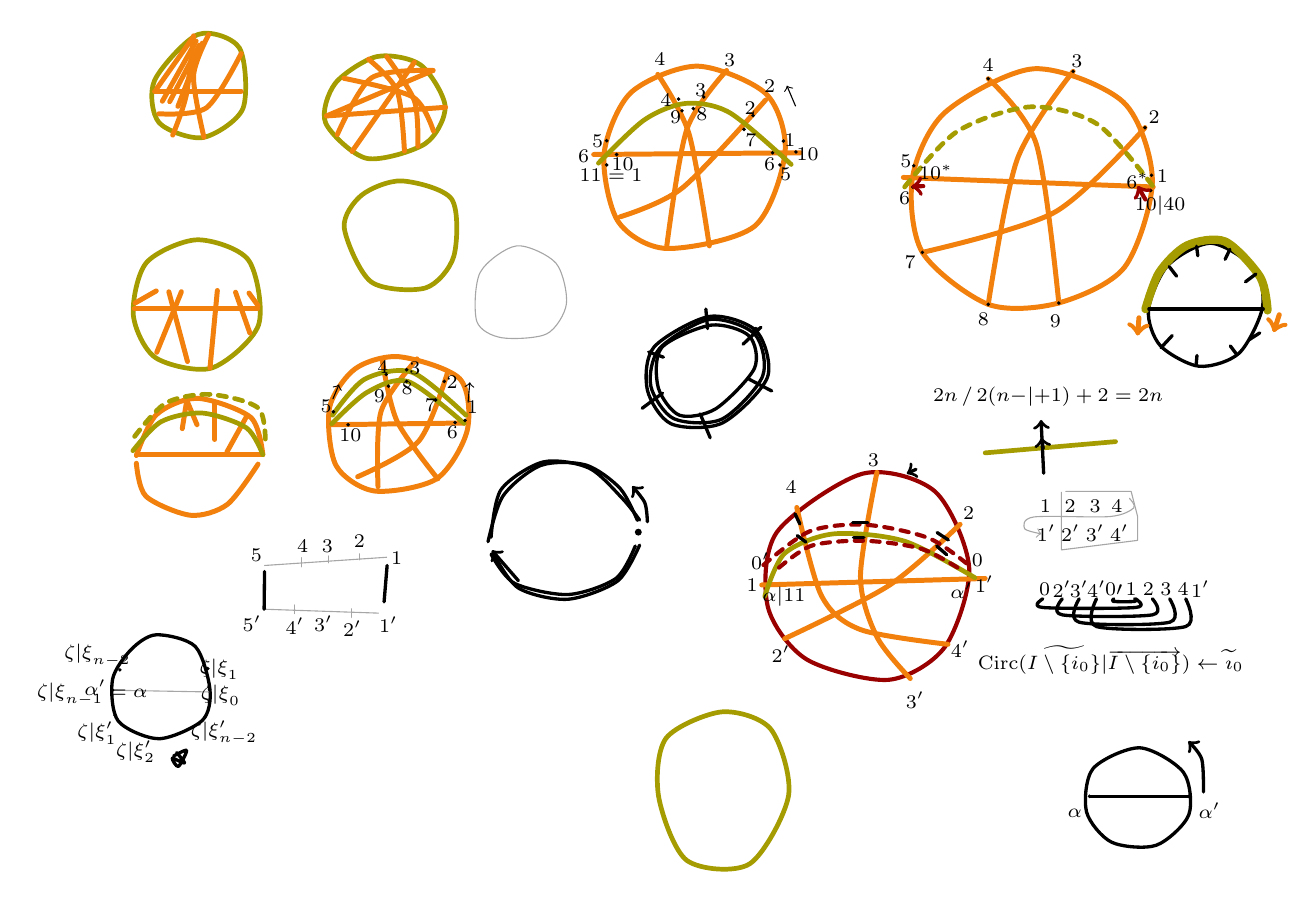
\begin{tikzpicture}[x=.55cm,y=-.55cm,line cap=round,line join=round,g/.style={olive!80!yellow,line width=1.7pt},r/.style={orange!80!brown,line width=1.8pt},w/.style={red!60!black,line width=1.5pt},b/.style={blue!60!black,line width=1.4pt},p/.style={gray!70,thin},k/.style={black,line width=1.2pt},every node/.style={font=\scriptsize}]
% E01-E06: six unlabelled small studies at left, including two empty outlines.
\draw[g] plot[smooth cycle] coordinates {(3.4,1.99) (4.36,2.3) (4.44,3.7) (3.51,4.37) (2.5,4.02) (2.4,3.05)};
\draw[r] plot[smooth] coordinates {(2.4,3.3) (4.4,3.3)};
\draw[r] plot[smooth] coordinates {(2.5,3.82) (3.6,3.68) (4.4,2.43)};
\draw[r] plot[smooth] coordinates {(3.65,1.99) (3.3,2.95) (3.54,4.36)};
\draw[r] plot[smooth] coordinates {(3.3,2.02) (3.13,3.4) (2.82,4.31)};
\draw[r] (2.45,3.24)--(3.27,2.08);
\draw[r] (2.58,3.53)--(3.36,2.14);
\draw[r] (2.75,3.54)--(3.43,2.24);
\draw[r] (2.94,3.65)--(3.5,2.19);
\draw[g] plot[smooth cycle] coordinates {(7.53,2.5) (8.54,2.69) (9.11,3.65) (8.65,4.51) (7.3,4.85) (6.35,4.03) (6.57,3.12)};
\draw[r] plot[smooth] coordinates {(6.37,3.87) (8.83,2.82)};
\draw[r] plot[smooth] coordinates {(6.37,3.87) (9.12,3.67)};
\draw[r] plot[smooth] coordinates {(6.77,3.0) (8.36,3.43) (8.84,4.22)};
\draw[r] plot[smooth] coordinates {(7.34,2.56) (8.0,3.29) (8.17,4.68)};
\draw[r] plot[smooth] coordinates {(7.76,2.5) (8.4,3.52) (8.48,4.57)};
\draw[r] plot[smooth] coordinates {(6.62,4.3) (7.41,2.99) (8.83,2.82)};
\draw[r] plot[smooth] coordinates {(6.96,4.69) (8.4,2.63)};
\draw[g] plot[smooth cycle] coordinates {(8.1,5.37) (9.26,5.79) (9.31,7.11) (8.66,7.84) (7.4,7.7) (6.78,6.45) (7.18,5.7)};
\draw[p] plot[smooth cycle] coordinates {(10.76,6.87) (11.67,7.27) (11.91,8.21) (11.46,8.9) (10.41,8.99) (9.84,8.61) (9.92,7.48)};
\draw[g] plot[smooth cycle] coordinates {(3.38,6.73) (4.57,7.2) (4.8,8.7) (3.72,9.69) (2.42,9.45) (1.91,8.47) (2.21,7.26)};
\draw[r] (1.93,8.32)--(4.78,8.32);
\draw[r] (1.95,8.19)--(2.44,7.91);
\draw[r] (2.45,9.33)--(3.02,7.93);
\draw[r] (2.73,7.93)--(3.16,9.54);
\draw[r] (3.85,7.9)--(3.68,9.69);
\draw[r] (4.27,7.94)--(4.6,8.88);
\draw[r] (4.58,7.96)--(4.79,8.25);
\draw[r] plot[smooth] coordinates {(1.98,11.71) (2.44,10.77) (3.39,10.39) (4.62,10.83) (4.9,11.69)};
\draw[r] plot[smooth] coordinates {(1.99,11.69) (4.9,11.69)};
\draw[r] plot[smooth] coordinates {(1.98,11.89) (2.2,12.65) (3.23,13.09) (4.08,12.84) (4.79,11.91)};
\draw[r] plot[smooth] coordinates {(3.14,10.46) (3.04,11.09)};
\draw[r] plot[smooth] coordinates {(3.15,10.45) (3.38,11.0)};
\draw[r] plot[smooth] coordinates {(3.79,10.49) (3.79,11.34)};
\draw[r] plot[smooth] coordinates {(4.53,10.8) (4.07,11.63)};
\draw[g] plot[smooth] coordinates {(1.9,11.6) (2.55,10.93) (3.5,10.73) (4.52,11.07) (4.9,11.69)};
\draw[g,dashed] plot[smooth] coordinates {(1.94,11.27) (2.66,10.5) (3.68,10.3) (4.8,10.62) (4.96,11.5)};
% E07: large upper-central numbered arrangement.
\draw[r] plot[smooth cycle] coordinates {(14.93,2.72) (16.52,3.36) (16.96,4.7) (16.25,6.42) (14.22,6.93) (13.1,6.3) (12.78,4.74) (13.4,3.33)};
\draw[r] plot[smooth] coordinates {(14.02,2.91) (14.74,4.28) (15.21,6.87)};
\draw[r] plot[smooth] coordinates {(15.61,2.82) (14.69,4.18) (14.22,6.93)};
\draw[r] plot[smooth] coordinates {(13.15,6.2) (14.59,5.53) (16.51,3.5)};
\draw[r] plot[smooth] coordinates {(12.54,4.76) (17.31,4.72)};
\draw[g] plot[smooth] coordinates {(12.65,4.96) (13.71,3.96) (14.67,3.58) (15.69,3.8) (17.1,4.99)};
\draw[->] plot[smooth] coordinates {(17.2,3.64) (17.0,3.17)};
\fill[black] (12.84,4.44) circle (.045);
\fill[black] (13.07,4.76) circle (.045);
\fill[black] (12.84,5.0) circle (.045);
\fill[black] (14.58,3.75) circle (.045);
\fill[black] (14.84,3.7) circle (.045);
\fill[black] (15.08,3.43) circle (.045);
\fill[black] (14.5,3.48) circle (.045);
\fill[black] (16.22,3.86) circle (.045);
\fill[black] (16.01,4.18) circle (.045);
\fill[black] (16.92,4.45) circle (.045);
\fill[black] (16.67,4.72) circle (.045);
\fill[black] (16.84,5.0) circle (.045);
\fill[black] (17.21,4.7) circle (.045);
\node at (12.63,4.46) {$5$};
\node at (12.31,4.8) {$6$};
\node at (12.94,5.24) {$11=1$};
\node at (13.21,4.98) {$10$};
\node at (14.43,3.91) {$9$};
\node at (15.04,3.84) {$8$};
\node at (16.17,4.42) {$7$};
\node at (16.6,4.98) {$6$};
\node at (16.97,5.21) {$5$};
\node at (17.07,4.42) {$1$};
\node at (17.48,4.75) {$10$};
\node at (16.15,3.7) {$2$};
\node at (16.6,3.18) {$2$};
\node at (15.01,3.27) {$3$};
\node at (15.68,2.58) {$3$};
\node at (14.21,3.5) {$4$};
\node at (14.07,2.57) {$4$};
% E08: upper-right arrangement, boundary numbering and starred labels.
\draw[r] plot[smooth cycle] coordinates {(22.71,2.78) (24.77,3.55) (25.44,5.35) (24.8,7.36) (23.27,8.19) (21.65,8.22) (20.13,7.02) (19.9,5.3) (20.65,3.79)};
\draw[r] plot[smooth] coordinates {(21.65,3.01) (22.76,4.52) (23.28,8.19)};
\draw[r] plot[smooth] coordinates {(23.61,2.84) (22.32,4.87) (21.65,8.22)};
\draw[r] plot[smooth] coordinates {(20.13,7.02) (23.19,6.09) (25.27,4.14)};
\draw[r] plot[smooth] coordinates {(19.69,5.29) (25.46,5.51)};
\draw[g,dashed] plot[smooth] coordinates {(19.72,5.51) (20.93,4.23) (22.62,3.66) (24.17,4.06) (25.46,5.5)};
\fill[black] (21.65,3.01) circle (.045);
\fill[black] (23.61,2.84) circle (.045);
\fill[black] (25.27,4.14) circle (.045);
\fill[black] (25.42,5.24) circle (.045);
\fill[black] (25.4,5.59) circle (.045);
\fill[black] (19.93,5.02) circle (.045);
\fill[black] (19.91,5.51) circle (.045);
\fill[black] (20.13,7.02) circle (.045);
\fill[black] (21.65,8.22) circle (.045);
\fill[black] (23.28,8.19) circle (.045);
\node at (21.65,2.71) {$4$};
\node at (23.7,2.61) {$3$};
\node at (25.48,3.9) {$2$};
\node at (25.67,5.26) {$1$};
\node at (25.62,5.94) {$\unsure{10|40}$};
\node at (19.75,4.91) {$5$};
\node at (19.72,5.76) {$6$};
\node at (19.85,7.24) {$7$};
\node at (21.54,8.56) {$8$};
\node at (23.2,8.62) {$9$};
\node at (20.44,5.17) {$10^*$};
\node at (25.1,5.37) {$6^*$};
\draw[w,->] plot[smooth] coordinates {(20.15,5.49) (19.88,5.5)};
\draw[w,->] plot[smooth] coordinates {(25.28,5.8) (25.1,5.49)};
% E09: small right circular count, marks and two orange arrows.
\draw[k] plot[smooth cycle] coordinates {(26.8,6.81) (27.8,7.4) (27.98,8.3) (27.44,9.35) (26.52,9.65) (25.62,9.17) (25.35,8.35) (25.8,7.32)};
\draw[g,line width=3pt] plot[smooth] coordinates {(25.28,8.33) (25.6,7.48) (26.24,6.86) (27.12,6.77) (27.93,7.59) (28.1,8.36)};
\draw[k] (25.36,8.33)--(28.0,8.33);
\draw[k] (25.83,7.35)--(26.0,7.57);
\draw[k] (26.46,6.88)--(26.49,7.1);
\draw[k] (27.23,6.95)--(27.12,7.18);
\draw[k] (27.83,7.52)--(27.59,7.7);
\draw[k] (27.92,8.88)--(27.67,9.04);
\draw[k] (27.39,9.38)--(27.24,9.18);
\draw[k] (26.45,9.63)--(26.47,9.4);
\draw[k] (25.64,9.22)--(25.9,8.94);
\draw[r,->] plot[smooth] coordinates {(25.13,8.53) (25.1,8.94)};
\draw[r,->] plot[smooth] coordinates {(28.37,8.46) (28.24,8.86)};
% E10: mid-left second numbered arrangement.
\draw[r] plot[smooth cycle] coordinates {(8.05,9.43) (9.45,9.94) (9.62,11.13) (8.91,12.25) (7.48,12.53) (6.59,11.94) (6.44,10.61) (7.03,9.71)};
\draw[r] plot[smooth] coordinates {(7.66,9.53) (8.0,10.92) (8.94,12.25)};
\draw[r] plot[smooth] coordinates {(8.46,9.48) (7.63,10.69) (7.56,12.43)};
\draw[r] plot[smooth] coordinates {(7.09,12.2) (8.5,11.38) (9.17,9.78)};
\draw[r] plot[smooth] coordinates {(6.45,11.0) (9.56,10.96)};
\draw[g] plot[smooth] coordinates {(6.51,10.78) (7.25,9.95) (8.35,9.79) (9.59,10.78)};
\draw[g] plot[smooth] coordinates {(6.49,10.98) (7.31,10.25) (8.25,10.0) (9.55,10.97)};
\draw[->] plot[smooth] coordinates {(6.52,10.4) (6.66,10.07)};
\draw[->] plot[smooth] coordinates {(9.64,10.48) (9.68,10.02)};
\fill[black] (6.53,10.7) circle (.045);
\fill[black] (6.87,11.0) circle (.045);
\fill[black] (7.75,9.84) circle (.045);
\fill[black] (7.8,10.11) circle (.045);
\fill[black] (8.22,9.73) circle (.045);
\fill[black] (8.22,10.0) circle (.045);
\fill[black] (9.09,10.0) circle (.045);
\fill[black] (8.89,10.43) circle (.045);
\fill[black] (9.34,10.95) circle (.045);
\fill[black] (9.57,10.9) circle (.045);
\node at (6.36,10.57) {$5$};
\node at (6.92,11.24) {$10$};
\node at (7.59,10.34) {$9$};
\node at (8.23,10.16) {$8$};
\node at (8.77,10.54) {$7$};
\node at (9.28,11.17) {$6$};
\node at (9.74,10.59) {$1$};
\node at (9.27,10.03) {$2$};
\node at (8.41,9.7) {$3$};
\node at (7.67,9.67) {$4$};
% E11 and E12: black circular studies with ticks, dot and directed arcs.
\draw[k] plot[smooth cycle] coordinates {(15.21,8.5) (16.3,8.84) (16.55,9.91) (15.51,10.96) (14.33,10.98) (13.78,10.2) (13.93,9.21)};
\draw[k] plot[smooth cycle] coordinates {(15.25,8.7) (16.13,8.95) (16.25,9.7) (15.36,10.63) (14.52,10.78) (14.03,10.14) (14.11,9.22)};
\draw[k] plot[smooth cycle] coordinates {(15.21,8.57) (16.26,8.91) (16.44,9.88) (15.5,10.87) (14.39,10.86) (13.86,10.11) (14.06,9.24)};
\draw[k] (13.81,9.32)--(14.15,9.44);
\draw[k] (15.13,8.33)--(15.17,8.78);
\draw[k] (15.0,10.75)--(15.23,11.3);
\draw[k] (13.66,10.62)--(14.13,10.27);
\draw[k] (16.13,9.95)--(16.65,10.22);
\draw[k] (15.99,9.14)--(16.4,8.75);
\fill[black] (16.28,8.82) circle (.08);
\draw[k] plot[smooth] coordinates {(10.1,13.7) (10.45,12.64) (11.32,11.94) (12.36,11.93) (13.15,12.47) (13.55,13.21)};
\draw[k] plot[smooth] coordinates {(13.6,13.78) (13.09,14.61) (11.94,15.03) (10.8,14.77) (10.21,13.95)};
\draw[k] plot[smooth] coordinates {(10.17,13.6) (10.4,12.5) (11.37,11.86) (12.43,12.0) (13.2,12.7) (13.6,13.2)};
\draw[k] plot[smooth] coordinates {(13.5,13.8) (13.05,14.55) (11.95,14.92) (10.71,14.66) (10.17,13.99)};
\draw[k,->] plot[smooth] coordinates {(13.78,13.24) (13.72,12.8) (13.43,12.42)};
\draw[k,->] plot[smooth] coordinates {(10.8,14.6) (10.19,13.9)};
\fill[black] (13.57,13.48) circle (.08);
% E13: middle-right divided count and crossing arrows.
\node at (23.03,10.35) {$2n\,/\,2(n\unsure{-|+}1)+2=2n$};
\draw[g] (21.58,11.65)--(24.59,11.39);
\draw[k,->] (22.93,12.12)--(22.87,10.89);
\draw[k,->] (22.92,11.55)--(22.88,11.3);
% E14: lower central coloured circle with primed numbers.
\draw[w] plot[smooth cycle] coordinates {(18.75,12.13) (20.42,12.54) (21.21,14.3) (20.65,16.13) (19.35,16.89) (17.46,16.42) (16.56,15.2) (16.77,13.48)};
\draw[r] plot[smooth] coordinates {(17.23,12.91) (17.8,14.95) (18.7,15.73) (20.72,16.07)};
\draw[r] plot[smooth] coordinates {(19.08,12.1) (18.7,14.5) (19.08,15.9) (19.85,16.86)};
\draw[r] plot[smooth] coordinates {(16.95,15.94) (19.36,14.71) (21.0,13.3)};
\draw[r] plot[smooth] coordinates {(16.42,14.7) (21.58,14.55)};
\draw[g] plot[smooth] coordinates {(16.49,14.96) (16.95,13.97) (18.08,13.52) (19.72,13.69) (21.34,14.53)};
\draw[w,dashed] plot[smooth] coordinates {(16.46,14.24) (17.53,13.46) (18.82,13.31) (20.28,13.62) (21.22,14.26)};
\draw[w,dashed] plot[smooth] coordinates {(16.82,14.3) (17.58,13.79) (18.81,13.68) (20.12,13.87) (21.07,14.38)};
\draw[k] (17.19,13.06)--(17.3,13.29);
\draw[k] (17.24,13.56)--(17.44,13.71);
\draw[k] (18.52,13.26)--(18.87,13.26);
\draw[k] (18.54,13.61)--(18.78,13.61);
\draw[k] (20.47,13.49)--(20.73,13.66);
\draw[k] (20.46,13.8)--(20.69,14.0);
\draw[k,->] plot[smooth] coordinates {(19.98,12.03) (19.77,12.13)};
\node at (17.1,12.45) {$4$};
\node at (19.0,11.82) {$3$};
\node at (21.2,13.04) {$2$};
\node at (21.4,14.12) {$0$};
\node at (21.56,14.68) {$1'$};
\node at (21.0,16.18) {$4'$};
\node at (19.96,17.36) {$3'$};
\node at (16.86,16.3) {$2'$};
\node at (16.2,14.7) {$1$};
\node at (16.39,14.15) {$0'$};
\node at (16.93,14.96) {$\unsure{\alpha|11}$};
\node at (21.03,14.83) {$\unsure{\alpha'}$};
% E15: left rectangular numbered strip.
\draw[p] (4.94,14.25)--(7.76,14.06);
\draw[p] (4.94,15.26)--(7.57,15.35);
\draw[k] (4.94,14.39)--(4.93,15.26);
\draw[k] (7.77,14.25)--(7.7,15.09);
\draw[p] (5.8,14.07)--(5.8,14.28);
\draw[p] (6.42,14.03)--(6.42,14.19);
\draw[p] (7.14,13.98)--(7.14,14.12);
\draw[p] (5.64,15.16)--(5.64,15.36);
\draw[p] (6.94,15.25)--(6.94,15.45);
\node at (4.75,14.02) {$5$};
\node at (5.82,13.81) {$4$};
\node at (6.39,13.8) {$3$};
\node at (7.13,13.69) {$2$};
\node at (7.99,14.08) {$1$};
\node at (4.65,15.59) {$5'$};
\node at (5.64,15.65) {$4'$};
\node at (6.3,15.6) {$3'$};
\node at (6.97,15.71) {$2'$};
\node at (7.8,15.62) {$1'$};
% E16: left lower circle with indexed Greek labels.
\draw[k] plot[smooth cycle] coordinates {(2.44,15.85) (3.34,16.12) (3.68,17.12) (3.5,17.83) (2.5,18.25) (1.56,17.84) (1.43,16.88) (1.86,16.19)};
\draw[p] (1.43,17.13)--(3.66,17.17);
\fill[black] (1.43,17.13) circle (.045);
\fill[black] (1.49,17.71) circle (.045);
\fill[black] (1.6,16.66) circle (.045);
\fill[black] (3.63,16.63) circle (.045);
\fill[black] (3.67,17.12) circle (.045);
\fill[black] (3.57,17.74) circle (.045);
\node at (1.08,16.32) {$\unsure{\zeta|\xi}_{n-2}$};
\node at (.96,17.23) {$\unsure{\zeta|\xi}_{n-1}=\unsure{\alpha}$};
\node at (1.03,17.07) {$\unsure{\alpha'}$};
\node at (1.07,18.12) {$\unsure{\zeta|\xi}'_1$};
\node at (1.96,18.55) {$\unsure{\zeta|\xi}'_2$};
\node at (3.89,16.64) {$\unsure{\zeta|\xi}_1$};
\node at (3.92,17.25) {$\unsure{\zeta|\xi}_0$};
\node at (4.0,18.11) {$\unsure{\zeta|\xi}'_{n-2}$};
\draw[k] plot[smooth] coordinates {(2.84,18.65) (3.14,18.52) (2.95,18.89) (2.81,18.7) (3.09,18.81) (2.91,18.57)};
% E17-E18: two order diagrams, and the arrowed circle at bottom right.
\node at (22.97,12.88) {$1$};
\node at (23.54,12.88) {$2$};
\node at (24.12,12.88) {$3$};
\node at (24.62,12.88) {$4$};
\node at (22.99,13.5) {$1'$};
\node at (23.55,13.5) {$2'$};
\node at (24.12,13.5) {$3'$};
\node at (24.68,13.5) {$4'$};
\draw[p] (23.44,12.54)--(24.95,12.54)--(25.1,13.12)--(25.1,13.67)--(23.34,13.89)--(23.34,12.56);
\draw[p,->] plot[smooth] coordinates {(24.91,12.7) (25.01,12.92) (24.46,13.12) (22.7,13.13) (22.49,13.4) (22.88,13.52)};
\node at (22.95,14.8) {$0$};
\node at (23.349999999999998,14.8) {$2'$};
\node at (23.75,14.8) {$3'$};
\node at (24.15,14.8) {$4'$};
\node at (24.55,14.8) {$\unsure{0}\prime$};
\node at (24.95,14.8) {$1$};
\node at (25.35,14.8) {$2$};
\node at (25.75,14.8) {$3$};
\node at (26.15,14.8) {$4$};
\node at (26.55,14.8) {$1'$};
\draw[k] plot[smooth] coordinates {(22.91,15.02) (22.91,15.22) (25.05,15.22) (25.05,15.02)};
\draw[k] plot[smooth] coordinates {(23.36,15.02) (23.36,15.39) (25.44,15.39) (25.44,15.02)};
\draw[k] plot[smooth] coordinates {(23.75,15.02) (23.75,15.56) (25.84,15.56) (25.84,15.02)};
\draw[k] plot[smooth] coordinates {(24.15,15.02) (24.15,15.66) (26.21,15.66) (26.21,15.02)};
\draw[k] plot[smooth] coordinates {(24.55,15.02) (24.55,15.08) (25.03,15.08) (25.03,15.02)};
\node at (24.48,16.43) {$\mathrm{Circ}(\unsure{\widetilde{I\setminus\{i_0\}}|\overrightarrow{I\setminus\{i_0\}}})\leftarrow\widetilde{\imath}_0$};
\draw[k] plot[smooth cycle] coordinates {(25.15,18.46) (26.16,19.03) (26.28,20.01) (25.53,20.71) (24.5,20.64) (23.92,19.94) (24.07,18.94)};
\draw[k] (23.99,19.58)--(26.28,19.58);
\draw[k,->] plot[smooth] coordinates {(26.62,19.48) (26.58,18.72) (26.27,18.31)};
\fill[black] (23.99,19.58) circle (.045);
\fill[black] (26.28,19.58) circle (.045);
\node at (23.65,19.98) {$\alpha$};
\node at (26.76,19.91) {$\alpha'$};
% E19: lower central empty green outline.
\draw[g] plot[smooth cycle] coordinates {(15.5,17.63) (16.63,18.03) (17.04,19.56) (16.14,21.14) (14.69,21.06) (14.04,19.59) (14.21,18.24)};
\end{tikzpicture}}

% E20: two-arrow diagram; the overwritten sign remains marked.
\diagram{\[\begin{tikzcd}[ampersand replacement=\&,column sep=large,row sep=large]
\widetilde{\Delta}_{\widetilde{\unsure{S|s}}}\arrow[r,"\varphi_0", "\sim"']\arrow[dr,"\varphi_1"'] \& \widetilde{\Delta}'_{\widetilde{\unsure{S|s}}'_0}\unsure{.}\\
\&\widetilde{\Delta}'_{\widetilde{\unsure{S|s}}_1}\deleted{\unsure{\xi}}
\end{tikzcd}\]}
% E21: labels and sequences below the left circle.
\[1\quad2\quad3\quad4\qquad1'\quad2'\quad3'\quad4'\]
\[\unsure{\zeta|\xi}_0\quad\unsure{\zeta|\xi}_1\quad\unsure{\zeta|\xi}_2\quad\unsure{\zeta|\xi}_3=\unsure{\zeta|\xi}_{n-1}.\]
\[\alpha\quad u^n\unsure{\zeta|\xi}_0,\ u^{n+1}\unsure{\zeta|\xi}_0,\ {-}\ u^{2(n-1)-1}\unsure{\zeta|\xi}_0\]
% E22: lower central sequence, with annotation written underneath.
\[\unsure{\zeta|\xi}_0\quad\unsure{\zeta|\xi}_1\quad {-}\quad\unsure{\zeta|\xi}_{n-2}\quad\underset{u^{n-1}}{\unsure{\zeta|\xi}_{n-1}}=\unsure{\zeta|\xi}'_0\]
% E23: lower-right two sequences and separate alpha.
\[\alpha,\ u^n\unsure{\zeta|\xi}_0,\ u^{n+1}\unsure{\zeta|\xi}_0,\ {-},\ u^{2n-2}\unsure{\zeta|\xi}_0\]
\[\alpha,\]
\[\unsure{\zeta|\xi}_0\quad\unsure{\zeta|\xi}_1\quad {-}\quad\unsure{\zeta|\xi}_{n-1}\quad\unsure{\bar\zeta_n|\bar\xi_n}=\unsure{\zeta|\xi}'_0\]
\margin{\mspage{131}}

\scanpage{133}
\margin{\uline{fuseau} \unsure{avec}
\[\left\{\begin{array}{ll}
\deleted{\unsure{b}}\inserted{a}&\text{des deux rives }\inserted{\text{(= côtés des \unsure{bigones})}}\text{ du fuseau}\\
\deleted{\unsure{\rho}}\inserted{\sigma}&\text{des deux extrémités}\\
\Omega&\text{\uline{des deux} orientations du fuseau}\\
&\boxed{\Omega\simeq a\wedge\sigma}\\
\unsure{\Omega'}&\text{ens des orientations de }X\text{ en le sommet du fuseau}
\end{array}\right.\]
\[\Omega'\simeq\Omega\wedge\sigma\simeq a\]
Si on a choisi un $D\in a$, alors $a\simeq\{\pm1\}$,
$\deleted{\unsure{\Longleftrightarrow}}\quad\Omega\simeq\sigma\simeq\omega$
(ens des orientations de $D$)}
\figure{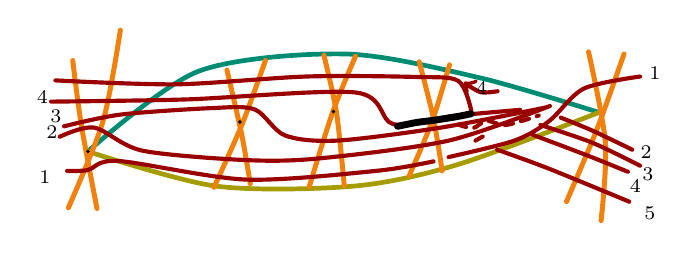
\begin{tikzpicture}[x=.55cm,y=-.55cm,line cap=round,line join=round,g/.style={olive!80!yellow,line width=1.7pt},r/.style={orange!80!brown,line width=1.8pt},w/.style={red!60!black,line width=1.5pt},b/.style={blue!60!black,line width=1.4pt},p/.style={gray!70,thin},k/.style={black,line width=1.2pt},every node/.style={font=\scriptsize}]
\draw[blue!45!green,line width=1.7pt] plot[smooth] coordinates {(3.65,5) (6.2,3.15) (9.6,2.75) (12.7,3.3) (15.45,4.1)};
\draw[olive!80!yellow,line width=1.7pt] plot[smooth] coordinates {(3.65,5) (6.6,5.8) (9.8,5.8) (12.2,5.3) (15.45,4.1)};
\draw[r] plot[smooth] coordinates {(3.3,2.9) (3.5,4.4) (3.86,6.32)};
\draw[r] plot[smooth] coordinates {(4.4,2.2) (4.0,4.3) (3.2,6.3)};
\draw[r] plot[smooth] coordinates {(6.86,3.12) (7.2,4.6) (7.4,5.75)};
\draw[r] plot[smooth] coordinates {(7.75,2.9) (7.2,4.4) (6.56,5.83)};
\draw[r] plot[smooth] coordinates {(9.1,2.78) (9.39,4.1) (9.57,5.79)};
\draw[r] plot[smooth] coordinates {(9.83,2.8) (9.3,4.1) (8.76,5.82)};
\draw[r] plot[smooth] coordinates {(11.3,2.93) (11.63,4.24) (11.83,5.45)};
\draw[r] plot[smooth] coordinates {(12.0,3.0) (11.6,4.3) (11.07,5.56)};
\draw[r] plot[smooth] coordinates {(15.21,2.7) (15.6,4.8) (15.5,6.6)};
\draw[r] plot[smooth] coordinates {(16.03,2.75) (15.4,4.5) (14.7,6.16)};
\draw[w] plot[smooth] coordinates {(2.9,3.36) (5.7,3.45) (8.7,3.27) (11.2,3.28) (12.2,3.37) (12.5,4.05)};
\draw[w] plot[smooth] coordinates {(2.8,3.85) (5.9,3.8) (9.84,3.64) (10.7,4.37) (12.1,4.18) (13.63,4.04)};
\draw[w] plot[smooth] coordinates {(3.1,4.42) (4.4,4.15) (6.5,4.0) (7.5,4.03) (8.2,4.63) (9.4,4.75) (11.8,4.45) (14.2,3.99)};
\draw[w] plot[smooth] coordinates {(3.0,4.66) (3.8,4.45) (4.9,4.98) (7.3,5.2) (9.0,5.16) (11.98,4.75) (14.32,3.95)};
\draw[w] plot[smooth] coordinates {(3.17,5.45) (3.65,5.43) (4.35,5.22) (7.3,5.65) (10.3,5.45) (11.63,5.23)};
\draw[w] plot[smooth] coordinates {(11.98,5.13) (13.5,4.75) (14.3,4.3) (15.1,3.55) (16.4,3.27)};
\draw[w] plot[smooth] coordinates {(14.57,4.22) (15.3,4.52) (16.22,4.96)};
\draw[w] plot[smooth] coordinates {(14.1,4.39) (15.3,4.8) (16.4,5.33)};
\draw[w] plot[smooth] coordinates {(13.93,4.62) (15.2,5.1) (16.12,5.47)};
\draw[w] plot[smooth] coordinates {(13.1,4.96) (14.3,5.4) (16.15,6.16)};
\draw[w,dashed] plot[smooth] coordinates {(12.2,4.38) (12.55,4.46) (12.85,4.29) (13.3,4.39) (14.06,4.17)};
\draw[w,dashed] plot[smooth] coordinates {(12.6,4.75) (12.9,4.58)};
\draw[k,line width=2.5pt] plot[smooth] coordinates {(10.8,4.42) (11.25,4.33) (11.64,4.28) (12.15,4.2) (12.5,4.13)};
\draw[w,->] plot[smooth] coordinates {(13.11,3.61) (12.71,3.63) (12.33,3.4)};
\fill[black] (3.65,5) circle (.045);
\fill[black] (7.16,4.32) circle (.045);
\fill[black] (9.32,4.08) circle (.045);
\fill[black] (11.63,4.25) circle (.045);
\node at (2.6,3.75) {$4$};
\node at (2.91,4.19) {$3$};
\node at (2.82,4.56) {$2$};
\node at (2.66,5.59) {$\unsure{1}$};
\node at (12.74,3.54) {$\unsure{4}$};
\node at (16.74,3.19) {$1$};
\node at (16.54,5.02) {$2$};
\node at (16.58,5.53) {$3$};
\node at (16.29,5.8) {$\unsure{4}$};
\node at (16.63,6.43) {$5$};
\end{tikzpicture}}
\uline{NB} ``fuseau'' $\longleftrightarrow$ p.r. \unsure{critique}, un sommet fixé dessus (``elt. de contact'')
\figure{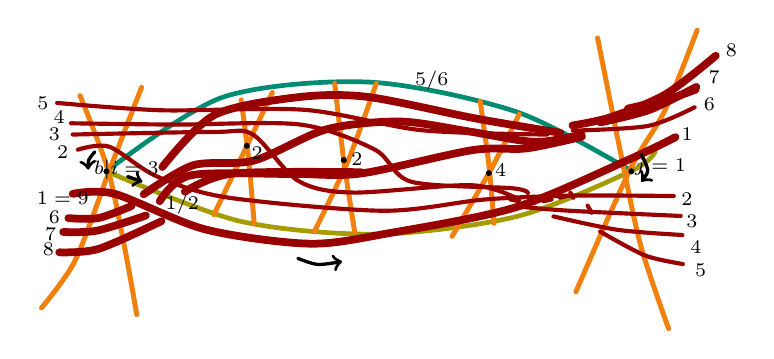
\begin{tikzpicture}[x=.55cm,y=-.55cm,line cap=round,line join=round,g/.style={olive!80!yellow,line width=1.7pt},r/.style={orange!80!brown,line width=1.8pt},w/.style={red!60!black,line width=1.5pt},b/.style={blue!60!black,line width=1.4pt},p/.style={gray!70,thin},k/.style={black,line width=1.2pt},every node/.style={font=\scriptsize}]
\draw[blue!45!green,line width=1.7pt] plot[smooth] coordinates {(5.72,10.85) (8.4,9.14) (11.8,8.79) (15.2,9.48) (17.84,10.84)};
\draw[olive!80!yellow,line width=1.7pt] plot[smooth] coordinates {(5.72,10.85) (8.8,12.0) (12.0,12.3) (15.2,11.89) (17.84,10.84) (18.39,10.4)};
\draw[r] plot[smooth] coordinates {(5.11,9.1) (5.75,10.8) (6.13,12.56) (6.42,14.16)};
\draw[r] plot[smooth] coordinates {(6.53,8.91) (5.8,10.8) (5.0,12.9) (4.22,14.0)};
\draw[r] plot[smooth] coordinates {(8.83,9.2) (9.0,10.54) (9.13,12.05)};
\draw[r] plot[smooth] coordinates {(9.55,9.03) (8.96,10.27) (8.2,11.85)};
\draw[r] plot[smooth] coordinates {(10.99,8.82) (11.2,10.6) (11.45,12.24)};
\draw[r] plot[smooth] coordinates {(11.95,8.82) (11.3,10.6) (10.52,12.24)};
\draw[r] plot[smooth] coordinates {(14.35,9.23) (14.55,10.7) (14.67,12.05)};
\draw[r] plot[smooth] coordinates {(15.25,9.53) (14.6,10.8) (13.7,12.35)};
\draw[r] plot[smooth] coordinates {(17.06,7.77) (17.6,10.46) (18.06,12.58) (18.7,14.48)};
\draw[r] plot[smooth] coordinates {(19.36,7.59) (18.61,9.45) (17.8,10.83) (16.56,13.63)};
\draw[w] plot[smooth] coordinates {(4.58,9.27) (7.0,9.44) (10.3,9.43) (13.0,9.9) (15.9,10.0)};
\draw[w] plot[smooth] coordinates {(4.9,9.74) (7.3,9.77) (10.2,9.77) (11.92,10.35) (12.76,11.09) (15.09,11.24) (15.45,11.35)};
\draw[w] plot[smooth] coordinates {(4.94,10.0) (8.2,9.94) (9.1,10.0) (10.15,11.07) (11.4,11.34) (14.15,11.17) (15.25,11.5)};
\draw[w] plot[smooth] coordinates {(5.06,10.35) (5.78,10.28) (6.87,10.96) (8.49,11.45) (12.1,11.76) (14.45,11.5) (16.5,11.41) (18.82,11.42)};
\draw[w] plot[smooth] coordinates {(15.31,11.67) (16.42,11.76) (18.98,11.88)};
\draw[w] plot[smooth] coordinates {(16.04,11.89) (17.52,12.2) (19.02,12.32)};
\draw[w] plot[smooth] coordinates {(17.12,12.24) (18.15,12.79) (19.03,12.99)};
\draw[w,line width=2.8pt] plot[smooth] coordinates {(4.94,11.37) (5.91,11.37) (8.0,12.19) (10.4,12.52) (12.23,12.28) (15.17,11.68) (17.8,10.57) (18.86,10.06)};
\draw[w,line width=2.8pt] plot[smooth] coordinates {(4.84,11.93) (5.53,11.93) (6.3,11.65)};
\draw[w,line width=2.8pt] plot[smooth] coordinates {(4.72,12.25) (5.5,12.22) (6.63,11.87)};
\draw[w,line width=2.8pt] plot[smooth] coordinates {(4.63,12.72) (5.54,12.64) (6.99,12.0)};
\draw[w,line width=2.8pt] plot[smooth] coordinates {(6.58,11.38) (7.72,10.71) (9.13,10.6) (10.8,9.88) (12.5,9.7) (14.1,9.93) (15.62,10.17) (16.69,10.0)};
\draw[w,line width=2.8pt] plot[smooth] coordinates {(6.95,11.54) (7.67,10.94) (10.01,10.91) (11.59,10.9) (14.17,10.36) (15.42,10.32) (16.7,10.05)};
\draw[w,line width=2.8pt] plot[smooth] coordinates {(7.53,11.32) (8.64,10.9) (11.6,10.87)};
\draw[w,line width=2.8pt] plot[smooth] coordinates {(7.01,10.75) (8.21,9.55) (10.12,9.14) (11.74,9.13) (14.25,9.63) (16.2,9.96)};
\draw[w,line width=2.8pt] plot[smooth] coordinates {(16.48,9.79) (17.36,9.6) (18.63,9.07) (19.79,8.18)};
\draw[w,line width=2.8pt] plot[smooth] coordinates {(17.13,9.72) (18.26,9.43) (19.34,8.9)};
\draw[w,line width=2.8pt] plot[smooth] coordinates {(17.76,9.4) (18.7,9.18) (19.33,8.96)};
\draw[w] plot[smooth] coordinates {(16.49,9.91) (18.23,9.8) (19.3,9.37)};
\draw[w,dashed] plot[smooth] coordinates {(15.05,11.5) (15.6,11.57) (16.34,11.42)};
\draw[w,dashed] plot[smooth] coordinates {(16.43,11.34) (16.5,11.46)};
\draw[w,dashed] plot[smooth] coordinates {(16.83,11.64) (17.0,11.94)};
\draw[k,->] plot[smooth] coordinates {(5.45,10.4) (5.31,10.59) (5.3,10.81)};
\draw[k,->] plot[smooth] coordinates {(6.21,10.97) (6.55,11.09)};
\draw[k,->] plot[smooth] coordinates {(10.14,12.86) (10.6,13.0) (11.16,12.93)};
\draw[k,->] plot[smooth] coordinates {(18.07,10.46) (18.22,10.83) (18.07,11.09)};
\fill[black] (5.72,10.85) circle (.07);
\fill[black] (8.96,10.26) circle (.07);
\fill[black] (11.2,10.59) circle (.07);
\fill[black] (14.55,10.89) circle (.07);
\fill[black] (17.84,10.85) circle (.07);
\node at (4.25,9.27) {$5$};
\node at (4.63,9.6) {$4$};
\node at (4.52,10.0) {$3$};
\node at (4.71,10.41) {$2$};
\node at (4.71,11.47) {$1=9$};
\node at (4.52,11.92) {$\unsure{6}$};
\node at (4.43,12.31) {$\unsure{7}$};
\node at (4.38,12.65) {$\unsure{8}$};
\node at (6.18,10.8) {$\unsure{b|i}=3$};
\node at (9.2,10.43) {$2$};
\node at (11.5,10.56) {$2$};
\node at (14.82,10.83) {$4$};
\node at (18.51,10.75) {$\unsure{j}=1$};
\node at (7.47,11.62) {$1/2$};
\node at (13.23,8.75) {$5/6$};
\node at (20.15,8.05) {$8$};
\node at (19.75,8.68) {$7$};
\node at (19.64,9.3) {$6$};
\node at (19.13,10.0) {$1$};
\node at (19.12,11.5) {$2$};
\node at (19.24,12.0) {$3$};
\node at (19.33,12.6) {$4$};
\node at (19.44,13.13) {$5$};
\end{tikzpicture}}
Ce circuit de positions relatives stables dépend de la position non-stable de départ $D$ \inserted{\unsure{avec le sommet} $s\in S_D$} (voir dessin), du choix de sa \unsure{quasiorientation} de degré $1$ i.e. de la rive correspondante $\rho$ de $D$ en $s$, et d'une \deleted{\unsure{co}}orientation $\omega$ de $D$ (pour indiquer l'ordre de succession des \deleted{\unsure{opérations}} balayages des triangles), ce qui (moyennant le choix de $\rho$) équivaut à la donnée d'une orientation $\bar\omega$ de $X$ en $s$.
\figure{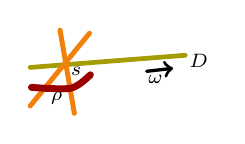
\begin{tikzpicture}[x=.55cm,y=-.55cm,line cap=round,line join=round,g/.style={olive!80!yellow,line width=1.7pt},r/.style={orange!80!brown,line width=1.8pt},w/.style={red!60!black,line width=1.5pt},b/.style={blue!60!black,line width=1.4pt},p/.style={gray!70,thin},k/.style={black,line width=1.2pt},every node/.style={font=\scriptsize}]
\draw[g] plot[smooth] coordinates {(21.2,13.92) (24.78,13.64)};
\draw[r] plot[smooth] coordinates {(21.89,13.06) (22.22,14.98)};
\draw[r] plot[smooth] coordinates {(22.57,13.13) (21.2,14.81)};
\draw[w,line width=2.5pt] plot[smooth] coordinates {(21.23,14.38) (22.14,14.4) (22.59,14.09)};
\draw[k,->] (23.89,14.01)--(24.5,13.94);
\node at (22.26,14.02) {$s$};
\node at (21.81,14.64) {$\rho$};
\node at (24.09,14.2) {$\omega$};
\node at (25.09,13.76) {$D$};
\end{tikzpicture}}
On trouve donc le circuit $D_1,D_2,{-}\ D_8,D_9=D_1$. Comment trouverait-on le circuit inverse \unsure{De} $D_1=D_9,D_8,{-}\ D_3,D_2$ ? C'est en changeant \uline{à la fois} la rive $\rho$, et l'orientation $\omega$.

Ainsi, l'opération $\sigma_2$ sur les repères de $\widetilde X$ correspond à l'opération qui \deleted{\unsure{change fixe}} \uline{fixe} $\bar\omega$ (orientation en $s$) et qui change $\omega$ (orientation de $D$, \deleted{\unsure{i.e. de}} \inserted{un} flanc du fuseau)
\figure{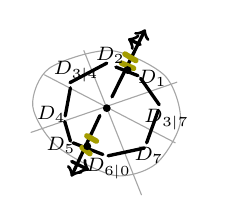
\begin{tikzpicture}[x=.55cm,y=-.55cm,line cap=round,line join=round,g/.style={olive!80!yellow,line width=1.7pt},r/.style={orange!80!brown,line width=1.8pt},w/.style={red!60!black,line width=1.5pt},b/.style={blue!60!black,line width=1.4pt},p/.style={gray!70,thin},k/.style={black,line width=1.2pt},every node/.style={font=\scriptsize}]
\draw[p] plot[smooth cycle] coordinates {(18.08,16.22) (19.34,16.8) (19.7,17.86) (19.13,18.84) (18.16,19.1) (16.85,18.43) (16.29,17.5) (16.67,16.63)};
\draw[p] (16.56,16.78)--(19.58,18.35);
\draw[p] (16.25,18.11)--(19.62,16.95);
\draw[p] (17.47,16.22)--(18.8,19.55);
\draw[k] plot[smooth] coordinates {(17.15,16.96) (18.0,16.51)};
\draw[k] plot[smooth] coordinates {(17.16,17.08) (17.04,17.73)};
\draw[k] plot[smooth] coordinates {(17.03,17.86) (17.16,18.31)};
\draw[k] plot[smooth] coordinates {(17.22,18.35) (17.91,18.62)};
\draw[k] plot[smooth] coordinates {(18.03,18.65) (18.87,18.47)};
\draw[k] plot[smooth] coordinates {(18.92,18.35) (19.19,17.6)};
\draw[k] plot[smooth] coordinates {(19.21,17.47) (18.78,16.86)};
\draw[k] plot[smooth] coordinates {(18.72,16.8) (18.21,16.6)};
\draw[k,->] plot[smooth] coordinates {(18.12,17.29) (18.89,15.73)};
\draw[k,->] plot[smooth] coordinates {(17.84,17.72) (17.18,19.13)};
\draw[g,line width=2pt] plot[smooth] coordinates {(18.34,16.51) (18.62,16.63)};
\draw[g,line width=2pt] plot[smooth] coordinates {(18.42,16.3) (18.67,16.45)};
\draw[g,line width=2pt] plot[smooth] coordinates {(17.54,18.19) (17.76,18.31)};
\draw[g,line width=2pt] plot[smooth] coordinates {(17.43,18.46) (17.61,18.6)};
\draw[k,->] plot[smooth] coordinates {(18.77,16.08) (18.49,15.95)};
\draw[k,->] plot[smooth] coordinates {(17.19,18.78) (17.59,18.98)};
\fill[black] (18.0,17.55) circle (.09);
\fill[black] (18.48,16.67) circle (.09);
\fill[black] (17.55,18.43) circle (.09);
\node at (18.08,16.33) {$D_2$};
\node at (19.05,16.87) {$D_1$};
\node at (19.38,17.82) {$D_{\unsure{3|7}}$};
\node at (18.97,18.64) {$D_{\unsure{7}}$};
\node at (18.04,18.94) {$D_{\unsure{6|0}}$};
\node at (16.94,18.41) {$D_5$};
\node at (16.72,17.69) {$D_{\unsure{4}}$};
\node at (17.29,16.71) {$D_{\unsure{3|4}}$};
\end{tikzpicture}}
Donner $(D,\bar\omega,\omega)$ revient \unsure{---} $\unsure{=}$ \unsure{que de} donner le fuseau qu'il définit, avec \deleted{\unsure{un} $\unsure{\omega}$} une \unsure{orientation} du fuseau $\Longleftrightarrow$ une orientation $\bar\omega$ de $X$ en \unsure{le|son} sommet, et un sommet (extrémité) du fuseau i.e. une \unsure{des|de} \unsure{Composantes}.
\margin{\mspage{132}}

\scanpage{134}
\margin{\unsure{1}}
\figure{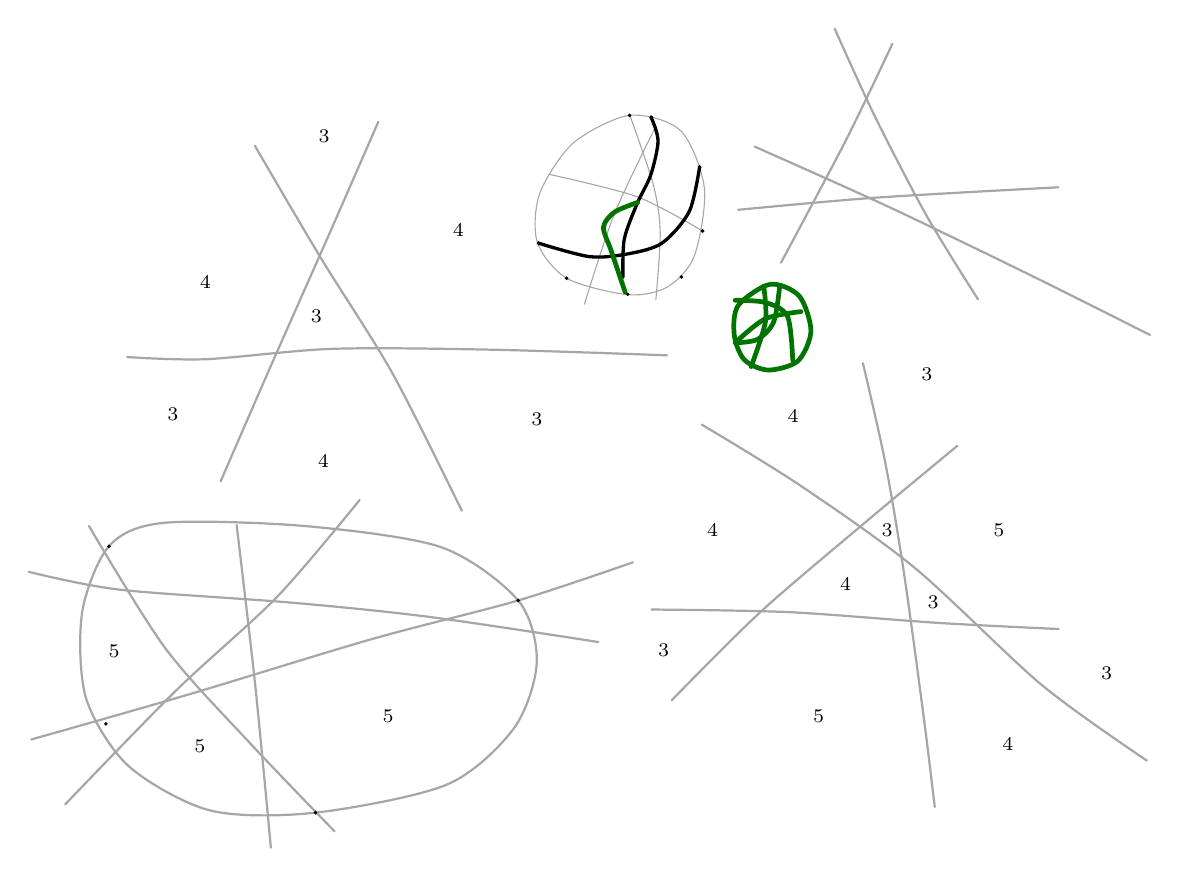
\begin{tikzpicture}[x=.55cm,y=-.55cm,line cap=round,line join=round,g/.style={green!45!black,line width=1.7pt},r/.style={orange!80!brown,line width=1.8pt},w/.style={red!60!black,line width=1.5pt},b/.style={blue!60!black,line width=1.4pt},p/.style={gray!70,thin},k/.style={black,line width=1.2pt},every node/.style={font=\scriptsize}]
\draw[p,line width=.8pt] plot[smooth] coordinates {(21.26,1.55) (22.2,3.6) (23.4,5.9) (24.57,7.8)};
\draw[p,line width=.8pt] plot[smooth] coordinates {(22.59,1.9) (21.53,4.1) (20.02,6.95)};
\draw[p,line width=.8pt] plot[smooth] coordinates {(19.41,4.27) (22.48,5.65) (25.7,7.2) (28.54,8.62)};
\draw[p,line width=.8pt] plot[smooth] coordinates {(19.03,5.73) (22.2,5.45) (26.42,5.21)};
\draw[p] plot[smooth cycle] coordinates {(16.52,3.55) (17.7,3.9) (18.25,5.23) (18.02,6.79) (17.4,7.51) (16.49,7.69) (15.07,7.31) (14.39,6.47) (14.45,5.35) (15.22,4.19)};
\draw[p] plot[smooth] coordinates {(14.66,4.91) (16.7,5.43) (18.21,6.22)};
\draw[p] plot[smooth] coordinates {(16.53,3.55) (17.07,5.15) (17.23,6.25) (17.13,7.8)};
\draw[p] plot[smooth] coordinates {(17.13,3.8) (16.17,5.83) (15.48,7.91)};
\draw[k] plot[smooth] coordinates {(17.02,3.59) (17.18,4.14) (17.01,4.93) (16.7,5.58) (16.4,6.41) (16.37,7.29)};
\draw[k] plot[smooth] coordinates {(14.42,6.5) (15.59,6.81) (16.47,6.75) (17.27,6.5) (17.9,5.77) (18.14,4.74)};
\draw[g] plot[smooth] coordinates {(16.71,5.56) (16.18,5.78) (15.92,6.13) (16.1,6.68) (16.42,7.63)};
\fill[black] (16.52,3.55) circle (.045);
\fill[black] (17.02,3.59) circle (.045);
\fill[black] (18.14,4.74) circle (.045);
\fill[black] (18.21,6.22) circle (.045);
\fill[black] (17.72,7.28) circle (.045);
\fill[black] (16.48,7.68) circle (.045);
\fill[black] (15.07,7.31) circle (.045);
\fill[black] (14.42,6.5) circle (.045);
\draw[p,line width=.8pt] plot[smooth] coordinates {(7.87,4.25) (9.38,6.82) (11.05,9.51) (12.65,12.68)};
\draw[p,line width=.8pt] plot[smooth] coordinates {(10.72,3.7) (9.64,6.17) (8.18,9.47) (7.08,12.0)};
\draw[p,line width=.8pt] plot[smooth] coordinates {(4.92,9.13) (6.73,9.18) (9.67,8.94) (13.34,8.96) (17.39,9.09)};
\node at (9.47,4.03) {$3$};
\node at (6.73,7.41) {$4$};
\node at (12.57,6.2) {$4$};
\node at (9.29,8.18) {$3$};
\node at (5.98,10.46) {$3$};
\node at (14.38,10.56) {$3$};
\node at (9.45,11.54) {$4$};
\draw[g] plot[smooth cycle] coordinates {(19.77,7.45) (20.44,7.72) (20.71,8.53) (20.41,9.22) (19.72,9.43) (19.17,9.19) (18.94,8.62) (19.03,7.94)};
\draw[g] plot[smooth] coordinates {(18.96,8.8) (19.65,8.25) (20.48,8.08)};
\draw[g] plot[smooth] coordinates {(18.99,8.8) (19.48,8.72) (19.85,8.32) (19.99,7.48)};
\draw[g] plot[smooth] coordinates {(19.33,9.35) (19.66,8.31) (19.62,7.49)};
\draw[g] plot[smooth] coordinates {(18.96,7.82) (19.66,7.87) (20.17,8.19) (20.29,9.2)};
\draw[p,line width=.8pt] plot[smooth] coordinates {(21.91,9.27) (22.42,11.53) (22.85,14.06) (23.3,17.33) (23.57,19.52)};
\draw[p,line width=.8pt] plot[smooth] coordinates {(18.19,10.69) (20.44,12.08) (23.11,14.0) (26.05,16.71) (28.47,18.45)};
\draw[p,line width=.8pt] plot[smooth] coordinates {(17.5,17.05) (19.53,15.03) (21.89,13.01) (24.09,11.18)};
\draw[p,line width=.8pt] plot[smooth] coordinates {(17.03,14.96) (20.2,15.02) (23.67,15.27) (26.43,15.41)};
\node at (23.39,9.53) {$3$};
\node at (20.3,10.49) {$4$};
\node at (18.44,13.12) {$4$};
\node at (22.47,13.12) {$3$};
\node at (25.05,13.14) {$5$};
\node at (23.53,14.8) {$3$};
\node at (21.51,14.38) {$4$};
\node at (17.31,15.91) {$3$};
\node at (20.89,17.43) {$5$};
\node at (25.26,18.06) {$4$};
\node at (27.54,16.42) {$3$};
\draw[p,line width=.8pt] plot[smooth cycle] coordinates {(4.5,13.5) (5.75,12.96) (9.0,13.03) (12.17,13.52) (13.95,14.75) (14.38,16.17) (13.86,17.69) (12.31,19.0) (9.27,19.65) (6.84,19.6) (4.95,18.57) (3.97,17.0) (3.88,15.04)};
\draw[p,line width=.8pt] plot[smooth] coordinates {(4.04,13.03) (5.8,15.85) (7.8,18.09) (9.71,20.08)};
\draw[p,line width=.8pt] plot[smooth] coordinates {(7.45,13.01) (7.88,16.72) (8.24,20.46)};
\draw[p,line width=.8pt] plot[smooth] coordinates {(10.29,12.43) (8.4,14.65) (6.05,16.83) (3.49,19.46)};
\draw[p,line width=.8pt] plot[smooth] coordinates {(2.71,17.96) (6.31,16.93) (10.58,15.64) (13.95,14.75) (16.6,13.87)};
\draw[p,line width=.8pt] plot[smooth] coordinates {(2.65,14.09) (4.74,14.5) (8.71,14.8) (11.9,15.13) (15.8,15.71)};
\fill[black] (4.5,13.5) circle (.045);
\fill[black] (13.95,14.75) circle (.045);
\fill[black] (9.27,19.65) circle (.045);
\fill[black] (4.43,17.6) circle (.045);
\node at (4.62,15.92) {$5$};
\node at (6.6,18.11) {$5$};
\node at (10.95,17.42) {$5$};
\end{tikzpicture}}
\margin{\mspage{133}}

\scanpage{135}
en somme, la donnée de $(D,\bar\omega,\omega)$ revient à celle du fuseau accompagné, avec une \unsure{épingle} de ce fuseau i.e. du bigone qu'il définit.
De ce point de vue, $\sigma_2$ est l'opération qui fixe \deleted{\unsure{le}} l'élém. de structure \inserted{d'un repère} de dim $1$ (\unsure{le mur}), et pas celui de dim $0$. Pour $\sigma_0$, serait-ce l'inverse ?

\uline{Non}, cette opération inverse, \deleted{\unsure{i.e.}} \unsure{ou donc} que je note $\sigma$ dans les repères de $\widetilde X$, est celle qui remplace un repère par son symétrique p.r. au \deleted{\unsure{l'}}\inserted{sommet} origine, qui commute bien à $\sigma_2$,
\diagram{\[\begin{tikzcd}[ampersand replacement=\&,column sep=small,row sep=small]
\sigma\arrow[r,dash]\arrow[dr,dash]\&\sigma_2\arrow[r,dash]\&\sigma_0\\
\&\sigma_1\&
\end{tikzcd}\]}
On a les quatre \unsure{disponibles|dispositions}
\diagram{\[\begin{tikzcd}[ampersand replacement=\&,column sep=small]
\overbrace{\sigma_1}^{\text{fuseaux locaux}},\&\overbrace{\sigma,\ \sigma_2}^{\text{fuseaux globaux}\leftrightarrow\text{\unsure{ds}}},\&\sigma_0
\end{tikzcd}\]}
sur les repères, dont deux consécutifs commutent. On vient d'interpréter $\sigma,\sigma_2$ comme opérations sur les fuseaux, il resterait à interpréter $\sigma_1$ et $\sigma_0$.

Pour $\sigma_1$, on trouve que les élémts de $\widetilde X^{\swarrow\!\searrow}/\sigma_1$, i.e. les secteurs angulaires de $\widetilde X$, correspondent aux figures formées par une p.r. stable (noire).
\deleted{\figure{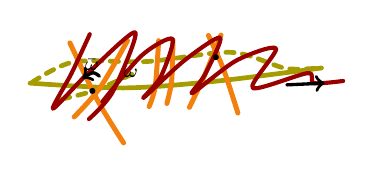
\begin{tikzpicture}[x=.55cm,y=-.55cm,line cap=round,line join=round,g/.style={olive!80!yellow,line width=1.7pt},r/.style={orange!80!brown,line width=1.8pt},w/.style={red!60!black,line width=1.5pt},b/.style={blue!60!black,line width=1.4pt},p/.style={gray!70,thin},k/.style={black,line width=1.2pt},every node/.style={font=\scriptsize}]
\draw[g] plot[smooth] coordinates {(14.87,3.14) (17.08,3.25) (19.21,3.09) (21.6,2.79)};
\draw[g,dashed] plot[smooth] coordinates {(14.92,3.12) (15.88,2.65) (17.59,2.64) (19.52,2.43) (20.78,2.8) (21.61,2.78)};
\draw[g,dashed] plot[smooth] coordinates {(15.6,3.51) (16.39,3.3) (17.38,2.86)};
\draw[r] plot[smooth] coordinates {(15.79,2.21) (16.43,3.54) (17.03,4.52)};
\draw[r] plot[smooth] coordinates {(17.12,2.16) (16.49,3.24) (15.89,3.92)};
\draw[r] plot[smooth] coordinates {(17.84,2.16) (17.76,3.22) (17.62,3.68)};
\draw[r] plot[smooth] coordinates {(18.17,2.14) (18.14,3.08) (18.03,3.61)};
\draw[r] plot[smooth] coordinates {(18.99,2.04) (19.33,2.8) (19.67,3.83)};
\draw[r] plot[smooth] coordinates {(19.28,2.03) (18.94,2.87) (18.55,3.7)};
\draw[w] plot[smooth] coordinates {(16.25,2.01) (15.83,2.91) (15.4,3.73) (16.23,2.89) (17.3,1.97) (16.78,3.34) (16.23,3.97)};
\draw[w] plot[smooth] coordinates {(16.54,3.57) (17.45,2.5) (18.16,2.12) (17.89,2.99) (17.49,3.48) (18.43,2.62) (19.26,2.09) (18.91,2.94) (18.62,3.37) (19.63,2.62) (20.55,2.34) (20.01,3.25) (21.28,2.91) (21.42,3.14) (22.1,3.09)};
\draw[k,->] (20.8,3.18)--(21.67,3.14);
\draw[k,->] plot[smooth] coordinates {(16.47,2.98) (16.32,2.9) (16.08,3.03)};
\fill[black] (16.31,3.32) circle (.07);
\fill[black] (19.16,2.54) circle (.07);
\node at (16.3,2.73) {$\unsure{\bar\omega}$};
\node at (17.2,2.91) {$\unsure{\omega}$};
\end{tikzpicture}}}
\figure{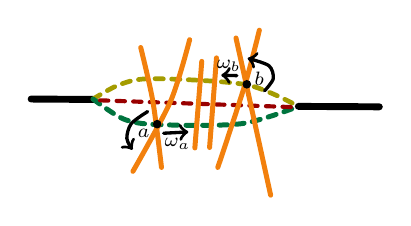
\begin{tikzpicture}[x=.55cm,y=-.55cm,line cap=round,line join=round,g/.style={olive!80!yellow,line width=1.7pt},r/.style={orange!80!brown,line width=1.8pt},w/.style={red!60!black,line width=1.5pt},b/.style={blue!60!black,line width=1.4pt},p/.style={gray!70,thin},k/.style={black,line width=1.2pt},every node/.style={font=\scriptsize}]
\draw[k,line width=2.5pt] (14.94,5.91)--(16.38,5.92);
\draw[k,line width=2.5pt] (21.11,6.08)--(22.98,6.09);
\draw[g,dashed] plot[smooth] coordinates {(16.37,5.91) (17.0,5.57) (17.76,5.44) (19.91,5.58) (21.11,6.08)};
\draw[blue!35!green!70!black,line width=1.8pt,dashed] plot[smooth] coordinates {(16.37,5.91) (17.07,6.37) (17.85,6.5) (19.79,6.48) (21.11,6.08)};
\draw[w,dashed] (16.53,5.94)--(21.07,6.1);
\draw[r] plot[smooth] coordinates {(17.47,4.72) (17.75,5.96) (17.95,7.49)};
\draw[r] plot[smooth] coordinates {(18.6,4.54) (18.16,5.96) (17.29,7.58)};
\draw[r] plot[smooth] coordinates {(18.88,5.04) (18.72,7.04)};
\draw[r] plot[smooth] coordinates {(19.22,4.96) (19.06,7.03)};
\draw[r] plot[smooth] coordinates {(19.67,4.5) (19.98,5.9) (20.47,8.13)};
\draw[r] plot[smooth] coordinates {(20.21,4.32) (19.88,5.57) (19.25,7.49)};
\fill[black] (17.85,6.49) circle (.1);
\fill[black] (19.92,5.57) circle (.1);
\draw[k,->] plot[smooth] coordinates {(17.63,6.2) (17.25,6.48) (17.15,6.82) (17.28,7.08)};
\draw[k,->] plot[smooth] coordinates {(20.33,5.72) (20.53,5.44) (20.43,5.14) (19.94,4.97)};
\draw[k,->] (18.0,6.7)--(18.57,6.67);
\draw[k,->] (19.69,5.37)--(19.33,5.36);
\node at (17.54,6.7) {$a$};
\node at (20.21,5.44) {$b$};
\node at (18.32,6.95) {$\omega_a$};
\node at (19.5,5.14) {$\omega_b$};
\end{tikzpicture}}
et deux triangles fermés ``\uline{anticonsécutifs}'', donnant naissance à \uline{deux} p.r. quasi-stables, chacune avec une orientation \deleted{\unsure{de D}} \uline{et} orientation \deleted{\unsure{de}} \inserted{de} $X$ en le sommet ($a$ ou $b$), \unsure{les deux étant identifiés} par une orientation du bigone Vert ; Sur \deleted{C'est} les fuseaux locaux, l'op. de $\sigma_1$ est la symétrie centrale, \deleted{celle de $\sigma_2$} Il faudrait comprendre aussi les éléments de $\widetilde X^{\swarrow\!\searrow}/(\sigma_1,\sigma)$, qui sont figurés en dessin en $\{D_{1/2},D_{2/3},D_{5/6},D_{6/7}$
\deleted{\figure{\begin{tikzpicture}[x=.55cm,y=-.55cm,line cap=round,line join=round,g/.style={olive!80!yellow,line width=1.7pt},r/.style={orange!80!brown,line width=1.8pt},w/.style={red!60!black,line width=1.5pt},b/.style={blue!60!black,line width=1.4pt},p/.style={gray!70,thin},k/.style={black,line width=1.2pt},every node/.style={font=\scriptsize}]
\draw[r] plot[smooth] coordinates {(16.49,15.78) (16.86,17.34) (17.43,18.98)};
\draw[r] plot[smooth] coordinates {(17.42,15.65) (16.85,17.26) (16.31,18.6)};
\draw[r] plot[smooth] coordinates {(19.56,15.78) (19.9,17.21) (20.24,18.72)};
\draw[r] plot[smooth] coordinates {(20.61,15.68) (19.91,17.19) (19.05,19.0)};
\draw[w,line width=2.6pt] plot[smooth] coordinates {(15.64,17.4) (16.86,17.25) (19.88,17.17) (22.95,17.35)};
\draw[w,dashed] plot[smooth] coordinates {(15.91,16.72) (16.84,16.76) (18.43,16.79) (19.87,16.76) (22.49,16.72)};
\draw[w,dashed] plot[smooth] coordinates {(15.54,16.97) (16.44,17.02) (16.86,17.25) (17.79,17.8) (18.94,17.8) (19.91,17.17) (21.72,17.84)};
\draw[w,dashed] plot[smooth] coordinates {(15.45,17.63) (16.26,17.52) (16.86,17.25) (17.68,16.85) (18.37,16.82) (19.91,17.17) (21.69,17.88)};
\draw[w,dashed] plot[smooth] coordinates {(16.06,17.76) (17.07,17.83) (18.35,17.87) (19.94,17.47) (21.09,17.45)};
\draw[p,line width=.8pt] plot[smooth] coordinates {(16.82,15.93) (16.59,16.96) (16.3,18.8)};
\draw[p,line width=.8pt] plot[smooth] coordinates {(18.17,16.02) (18.83,15.78) (21.57,15.75)};
\draw[p,line width=.8pt] plot[smooth] coordinates {(20.04,17.0) (21.66,17.95) (21.78,19.1)};
\draw[k] plot[smooth] coordinates {(16.96,15.77) (16.16,16.98) (15.54,18.1) (17.49,15.87) (16.17,18.18) (18.65,15.89) (17.71,17.76) (19.99,16.05) (19.21,17.74) (21.45,16.2) (20.23,17.7) (23.61,16.49) (22.7,17.6) (25.17,16.93) (24.2,17.85) (26.35,17.68) (26.78,17.89)};
\fill[black] (16.86,17.25) circle (.09);
\fill[black] (19.91,17.17) circle (.09);
\node at (15.51,17.67) {$1$};
\node at (20.2,17.01) {$b$};
\node at (18.38,17.36) {$\text{arête}$};
\node at (18.32,17.72) {$\text{de }D$};
\node at (24.69,17.39) {$\text{p.r. critique }D$};
\node at (23.54,18.04) {$\text{avec}$};
\end{tikzpicture}}}
\margin{\mspage{134}}
\margin{\unsure{fus} $\leftarrow$ \unsure{fus}\par
sommets $\longleftrightarrow$ droites\par
arêtes $\longleftrightarrow$ bisect. ang. locaux}

\scanpage{136}
Sur $\widetilde X^{\swarrow\!\searrow}$, il y a les opérations
$\sigma_1,\sigma,\sigma_2,\sigma_0$ dont deux consécutifs commutent.
\figure{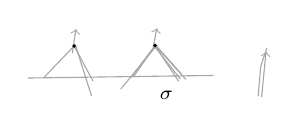
\begin{tikzpicture}[x=.55cm,y=-.55cm,line cap=round,line join=round,g/.style={olive!80!yellow,line width=1.7pt},r/.style={orange!80!brown,line width=1.8pt},w/.style={red!60!black,line width=1.5pt},b/.style={blue!60!black,line width=1.4pt},p/.style={gray!70,thin},k/.style={black,line width=1.2pt},every node/.style={font=\scriptsize}]
\draw[p] (17.98,1.73)--(22.25,1.67);
\draw[p] (18.34,1.72)--(19.04,.99)--(19.47,1.79);
\draw[p] (20.35,1.72)--(20.91,.98)--(21.62,1.76);
\draw[p] (20.12,1.98)--(20.91,1.02)--(21.49,1.75);
\draw[p] (20.41,1.7)--(20.92,.97)--(21.52,1.64);
\draw[p,->] (19.0,1.15)--(19.08,.6);
\draw[p,->] (20.86,1.05)--(20.95,.58);
\draw[p,->] (23.37,2.16)--(23.47,1.12);
\draw[p] (19.07,.97)--(19.44,2.14);
\draw[p] (20.92,1.0)--(21.45,1.8);
\draw[p] (23.29,2.14)--(23.35,1.45)--(23.49,1.04);
\fill[black] (19.04,.99) circle (.045);
\fill[black] (20.91,.98) circle (.045);
\node at (21.17,2.12) {$\unsure{\sigma}$};
\end{tikzpicture}}
\uline{faces de $\widetilde X$} : p.r. stables ; \uline{faces orientées} : p.r. orientées stables

\uline{arêtes de $\widetilde X$} : p.r. semi-stables ; \deleted{arêtes biorientées}

\uline{arêtes biorientées} i.e. repères : \deleted{\unsure{drapeaux}}\inserted{repères}
\[(D,s,\omega\inserted{,\bar\omega})\quad\text{où}\quad\left|\begin{array}{l}
D\text{ p.r. critique}\\
s\in S_D=D\cap S\\
\omega\text{ orientation de }D,\ \bar\omega\text{ ori. de }X\text{ en }s
\end{array}\right.\]
\inserted{ou \uline{repères}}
\[\text{i.e.}\quad\text{\unsure{Donc|Donner} \uline{repère p.r. :}}\quad(\unsure{D},S_D),+\]

\uline{Sommets} \deleted{$\unsure{\varphi}$} : \uline{p.r. critiques}

\uline{Sommets orientés} : p.r. \uline{orientées} critiques

\diagram{\[\begin{tikzcd}[ampersand replacement=\&,column sep=large]
\underset{\unsure{\varepsilon}}{\text{repères}}\arrow[r]\&\text{faces orientées}
\end{tikzcd}\]}
\[\deleted{\unsure{D}}(D,s,\omega)\longmapsto\text{la position relative stable obtenue en }\deleted{\text{\unsure{mouvant}}}\]
\margin{\mspage{135}}

\scanpage{137}
\begin{center}\ttfamily\scriptsize
PAGE 1\quad ON=CELMPQRSTV\quad08/19/82-15:20:31\quad CFT 1.09(06/28/82)\quad PAGE 1
\begin{tabular}{rrrl}
1&1.&&PROGRAM CRAY7\\
2&2.&&WRITE(6,1)\\
3&3.&1&FORMAT(' BONJOUR')\\
4&4.&&STOP\\
5&5.&&END
\end{tabular}\end{center}
\figure{\begin{tikzpicture}[x=.55cm,y=-.55cm,line cap=round,line join=round,g/.style={olive!80!yellow,line width=1.7pt},r/.style={orange!80!brown,line width=1.8pt},w/.style={red!60!black,line width=1.5pt},b/.style={blue!60!black,line width=1.4pt},p/.style={gray!70,thin},k/.style={black,line width=1.2pt},every node/.style={font=\scriptsize}]
\draw[p] (2.06,3.17)--(5.22,1.23);
\draw[p] (3.27,3.42)--(6.98,1.28);
\draw[p] (12.6,3.05)--(18.15,2.42);
\draw[p] (14.07,1.7)--(14.79,3.4);
\draw[p] (14.47,1.69)--(13.37,3.19);
\draw[p] (17.02,1.52)--(17.66,2.81);
\draw[p] (17.3,1.58)--(16.3,3.01);
\draw[p] (13.62,2.86)--(14.03,2.24);
\draw[p] (13.71,2.9)--(14.12,2.29);
\draw[p] (13.83,2.92)--(14.23,2.37);
\draw[p] (13.94,2.92)--(14.32,2.48);
\draw[p] (14.08,2.94)--(14.4,2.6);
% Small left orientation study.
\draw[p] (2.12,7.16)--(4.02,8.87);
\draw[p] (3.48,6.57)--(2.32,8.43);
\draw[p] (2.03,7.79)--(5.42,7.19);
\draw[k,line width=3pt] (4.15,6.99)--(4.27,7.92);
\draw[k,->] (4.51,7.81)--(4.49,7.02);
\draw[k,->] (4.47,7.59)--(5.17,7.56);
\draw[p,->] (2.4,10.32)--(2.66,9.09);
\node at (4.41,6.72) {$\unsure{\rho}$};
\node at (4.8,6.96) {$\omega$};
\node at (5.38,7.54) {$\bar\omega$};
% Large upper elongated arrangement.
\draw[r] plot[smooth] coordinates {(5.46,8.8) (6.23,6.9) (8.44,4.96) (11.13,4.4) (13.91,4.88) (15.76,6.23) (17.59,8.76)};
\draw[blue!35!green!70!black,line width=1.7pt] plot[smooth] coordinates {(5.46,8.8) (6.47,7.83) (8.11,7.5) (10.59,7.41) (12.89,7.26) (14.5,7.07) (16.02,7.63) (17.59,8.76)};
\draw[g] plot[smooth] coordinates {(5.46,8.8) (6.34,9.02) (9.42,9.05) (12.64,9.03) (15.41,8.81) (18.12,8.59)};
\draw[w,dashed] plot[smooth] coordinates {(5.46,8.8) (7.62,7.72) (9.53,7.77) (12.6,7.68) (14.5,7.36) (15.92,7.69) (17.59,8.76)};
\draw[w,dashed] plot[smooth] coordinates {(5.46,8.8) (6.39,9.25) (8.82,9.7) (10.91,9.82) (12.37,9.85) (15.04,9.25) (17.59,8.76)};
\draw[r] plot[smooth] coordinates {(5.14,8.13) (5.93,9.78)};
\draw[r] plot[smooth] coordinates {(5.81,7.83) (5.04,9.88)};
\draw[r] plot[smooth] coordinates {(17.39,8.0) (17.78,9.22)};
\draw[r] plot[smooth] coordinates {(18.14,7.8) (17.31,9.37)};
\draw[g] plot[smooth] coordinates {(7.43,6.57) (7.67,8.25) (8.05,9.67) (8.2,11.36)};
\draw[g] plot[smooth] coordinates {(7.98,6.35) (7.63,7.73) (6.67,9.97) (6.64,11.17)};
\draw[g] plot[smooth] coordinates {(8.4,6.36) (8.19,7.7) (8.41,10.2) (8.46,11.44)};
\draw[g] plot[smooth] coordinates {(8.75,6.1) (8.59,7.52) (8.65,8.69) (8.87,9.76) (8.88,10.06)};
\draw[g] plot[smooth] coordinates {(9.77,6.03) (9.79,6.62) (9.53,7.95) (8.74,10.06)};
\draw[g] plot[smooth] coordinates {(10.03,6.01) (10.06,7.2) (9.83,8.73) (9.38,10.68)};
\draw[g] plot[smooth] coordinates {(10.58,5.98) (10.38,6.75) (10.6,7.65) (11.1,9.07) (11.37,10.04)};
\draw[g] plot[smooth] coordinates {(11.02,6.12) (10.82,7.18) (10.14,9.11) (9.64,11.07)};
\draw[g] plot[smooth] coordinates {(11.6,6.15) (11.73,7.49) (12.01,8.63) (12.37,9.85) (12.46,10.67)};
\draw[g] plot[smooth] coordinates {(13.89,6.17) (13.29,7.66) (12.76,9.19) (11.82,11.23)};
\draw[g] plot[smooth] coordinates {(14.32,6.56) (14.53,7.34) (14.86,9.02) (15.31,10.72)};
\draw[g] plot[smooth] coordinates {(15.01,6.38) (14.51,7.35) (14.19,9.02) (13.83,10.5)};
\draw[p,line width=.8pt] (5.96,11.09)--(11.42,3.87);
\draw[p,line width=.8pt] (9.06,10.83)--(13.79,4.54);
\draw[p,line width=.8pt] (12.46,10.11)--(14.08,8.0);
\fill[black] (5.46,8.8) circle (.065);
\fill[black] (7.62,7.72) circle (.065);
\fill[black] (8.82,9.7) circle (.065);
\fill[black] (10.6,7.65) circle (.065);
\fill[black] (12.37,9.85) circle (.065);
\fill[black] (14.5,7.36) circle (.065);
\fill[black] (17.59,8.76) circle (.065);
% Upper right loop, crossing arcs and hatching; faint construction below.
\draw[g] plot[smooth] coordinates {(18.42,6.82) (19.35,6.4) (21.21,6.0) (22.13,6.45) (23.1,7.96) (24.45,8.72) (26.25,8.43) (27.55,7.68) (28.5,7.6)};
\draw[blue!35!green!70!black,line width=1.7pt] plot[smooth] coordinates {(18.42,6.82) (19.41,7.54) (20.38,7.81) (21.56,7.82) (23.11,7.21) (24.97,6.7) (26.52,7.41) (28.56,7.63)};
\draw[r] plot[smooth] coordinates {(17.17,6.28) (17.78,7.6)};
\draw[r] plot[smooth] coordinates {(17.66,5.99) (17.16,7.47)};
\draw[r] plot[smooth] coordinates {(18.22,5.88) (17.91,7.19)};
\draw[r] plot[smooth] coordinates {(18.05,6.07) (18.5,7.19)};
\draw[r] plot[smooth] coordinates {(21.22,5.11) (21.57,7.18) (22.06,9.71)};
\draw[r] plot[smooth] coordinates {(22.28,4.79) (21.63,6.92) (20.77,9.23)};
\draw[r] plot[smooth] coordinates {(23.8,4.84) (24.22,7.55) (24.66,9.58)};
\draw[r] plot[smooth] coordinates {(24.96,5.33) (24.41,7.69) (23.61,9.89)};
\draw[r] plot[smooth] coordinates {(28.0,6.66) (28.28,8.17)};
\draw[r] plot[smooth] coordinates {(28.24,6.59) (27.6,8.05)};
\draw[k] plot[smooth] coordinates {(23.7,4.65) (22.79,4.56) (21.72,4.79) (20.6,5.43) (19.98,6.42) (19.89,7.98) (20.27,8.86) (21.2,9.56) (22.66,9.93) (24.17,9.87)};
\draw[k] plot[smooth] coordinates {(24.2,9.67) (25.07,9.12) (25.64,8.2) (25.75,6.87) (25.46,5.94) (24.96,5.33)};
\draw[p] plot[smooth] coordinates {(19.9,6.24) (21.44,5.72) (22.95,5.59) (24.48,6.03) (25.77,6.76)};
\draw[p] (21.46,5.72)--(21.37,6.07);
\draw[p] (21.56,5.69)--(21.45,6.19);
\draw[p] (21.68,5.69)--(21.53,6.3);
\draw[p] (21.78,5.7)--(21.62,6.36);
\draw[p] (24.12,5.94)--(24.04,6.45);
\draw[p] (24.22,5.98)--(24.1,6.62);
\draw[p] (24.34,6.0)--(24.18,6.71);
\draw[p] (24.45,6.04)--(24.28,6.67);
\draw[p] (24.55,6.09)--(24.38,6.64);
\draw[k] plot[smooth] coordinates {(17.45,6.34) (18.06,5.89) (17.14,7.09) (18.17,5.87) (17.48,6.96) (18.31,5.9) (17.94,6.82) (18.74,6.81)};
\draw[k,->] (23.22,6.94)--(23.85,6.65);
\draw[k,->] (28.27,7.65)--(28.64,7.64);
\draw[k,->] (19.9,8.14)--(19.89,7.98);
\node at (23.52,5.32) {$D_1=D_{\unsure{19}}$};
\node at (19.46,7.94) {$\widehat D_4$};
\node at (21.26,6.96) {$s_4$};
\node at (22.7,6.57) {$D_{18}$};
\node at (24.67,7.83) {$t_3$};
\node at (28.28,7.26) {$\unsure{s_5}=19\ !$};
\node at (22.98,9.39) {$\unsure{D_5}\ \unsure{D_{19}}$};
\node[draw,circle,inner sep=.5pt] at (21.48,7.59) {$4$};
\node[draw,circle,inner sep=.5pt] at (24.3,8.44) {$18$};
\draw[p] (19.46,11.62)--(20.06,9.83)--(21.02,11.12);
\draw[p] (22.37,11.45)--(22.83,9.93)--(23.78,11.04);
\draw[p] (24.72,10.98)--(24.85,9.82)--(25.67,10.84);
\draw[g] (25.78,10.13)--(25.9,9.69);
\draw[p,->] plot[smooth] coordinates {(19.27,11.15) (19.34,11.63) (19.61,11.94) (19.46,12.19)};
\node at (22.41,12.61) {$s_4$};
% Middle slanting studies, with arrows and abbreviated caption.
\draw[g] plot[smooth] coordinates {(7.99,12.74) (10.34,12.08) (13.12,11.62) (15.44,11.48)};
\draw[g] plot[smooth] coordinates {(2.03,14.16) (3.34,13.71) (4.61,13.43) (5.7,13.27) (7.3,13.24)};
\draw[r] plot[smooth] coordinates {(10.61,10.87) (11.47,12.25)};
\draw[r] plot[smooth] coordinates {(11.2,10.75) (10.2,12.64)};
\draw[r] plot[smooth] coordinates {(11.15,10.05) (12.22,12.15)};
\draw[r] plot[smooth] coordinates {(11.52,9.97) (10.94,11.01)};
\draw[r] plot[smooth] coordinates {(3.99,12.49) (5.36,14.53)};
\draw[r] plot[smooth] coordinates {(5.14,12.08) (3.96,14.95)};
\draw[r] plot[smooth] coordinates {(6.69,11.91) (7.58,13.49)};
\draw[r] plot[smooth] coordinates {(7.27,12.04) (6.38,13.99)};
\draw[p] plot[smooth] coordinates {(12.72,10.4) (13.94,12.18)};
\draw[p] plot[smooth] coordinates {(13.02,10.51) (12.53,12.85)};
\draw[p] plot[smooth] coordinates {(5.88,11.17) (6.2,15.01)};
\draw[p] plot[smooth] coordinates {(6.03,11.62) (6.49,15.16)};
\draw[p] plot[smooth] coordinates {(2.76,14.69) (5.13,12.93) (7.41,12.19) (10.58,11.15)};
\draw[k,->] (12.37,12.07)--(13.68,11.86);
\draw[k,->] (5.23,13.52)--(5.2,13.07);
\draw[k,->] (5.15,13.3)--(5.8,13.27);
\draw[k,->] (4.99,13.0)--(4.78,12.85)--(4.48,12.86);
\fill[black] (4.61,13.43) circle (.08);
\node at (4.57,12.58) {$\bar\omega$};
\node at (5.28,12.85) {$\omega$};
\node at (16.45,11.72) {$\text{p.r. s.o.}$};
% Lower left small circled strip.
\draw[g] plot[smooth] coordinates {(1.86,17.28) (3.7,16.69) (5.5,16.4) (7.3,16.51)};
\draw[r] plot[smooth] coordinates {(3.34,16.0) (4.42,17.98)};
\draw[r] plot[smooth] coordinates {(3.97,15.64) (3.28,18.4)};
\draw[r] plot[smooth] coordinates {(4.5,16.14) (4.52,16.92)};
\draw[r] plot[smooth] coordinates {(4.94,16.04) (4.98,16.81)};
\draw[r] plot[smooth] coordinates {(5.31,16.04) (5.36,16.71)};
\draw[r] plot[smooth] coordinates {(5.63,15.7) (6.6,17.75)};
\draw[r] plot[smooth] coordinates {(6.37,15.42) (5.74,17.67)};
\draw[p] plot[smooth cycle] coordinates {(3.02,16.43) (4.6,15.66) (6.38,15.59) (6.99,16.15) (6.76,16.79) (5.08,17.15) (3.17,17.33) (2.85,16.9)};
\draw[p] plot[smooth] coordinates {(2.47,17.74) (6.64,15.98)};
\draw[p] plot[smooth] coordinates {(3.2,18.65) (3.43,17.39) (3.77,16.26)};
\draw[p] plot[smooth] coordinates {(4.22,18.62) (3.74,16.75)};
\draw[p] plot[smooth] coordinates {(3.24,17.29) (6.53,17.01)};
\draw[p] plot[smooth] coordinates {(3.35,16.34) (4.05,15.82)};
\draw[k] plot[smooth] coordinates {(4.14,16.15) (4.38,15.71) (4.5,15.72) (4.25,16.1) (4.55,15.67) (4.67,15.7) (4.45,16.11)};
\draw[k,->] (4.05,16.87)--(4.08,16.38);
\draw[k,->] (4.03,16.61)--(4.38,16.59);
\draw[k,->] (5.74,16.45)--(5.42,16.45);
\draw[k,->] (6.11,16.06)--(6.4,16.04);
\fill[black] (3.71,16.69) circle (.08);
\fill[black] (5.99,16.41) circle (.08);
\node at (4.96,15.53) {$\text{\unsure{avec sens prolongé}}$};
\draw[g] (3.33,15.4)--(3.34,15.63);
\draw[g] (3.14,15.34)--(3.15,15.57);
% Large lower arrangement and its individually written labels.
\draw[r] plot[smooth] coordinates {(9.26,16.87) (11.29,14.73) (13.9,13.25) (15.41,13.35) (17.66,14.73) (20.53,16.85) (22.16,15.31)};
\draw[r] plot[smooth] coordinates {(9.26,16.87) (10.44,18.55) (12.7,19.63) (14.7,19.84) (17.05,19.45) (19.03,18.46) (20.53,16.85) (22.19,18.11)};
\draw[r] plot[smooth] coordinates {(8.47,15.38) (9.26,16.87) (10.5,18.44)};
\draw[r] plot[smooth] coordinates {(8.26,18.4) (9.26,16.87)};
\draw[blue!35!green!70!black,line width=1.8pt] plot[smooth] coordinates {(9.26,16.87) (10.15,15.83) (11.38,15.38) (13.4,15.55) (15.72,15.8) (18.04,15.95) (19.32,16.31) (20.53,16.85)};
\draw[g] plot[smooth] coordinates {(9.26,16.87) (11.7,17.01) (15.27,17.03) (18.63,17.03) (20.53,16.85)};
\draw[g] plot[smooth] coordinates {(9.26,16.87) (10.92,17.69) (13.09,18.06) (15.67,18.28) (17.91,18.02) (20.53,16.85)};
\draw[w,dashed] plot[smooth] coordinates {(9.26,16.87) (11.38,15.67) (13.05,16.14) (14.26,16.16) (15.72,16.17) (17.86,16.3) (20.53,16.85)};
\draw[w,dashed] plot[smooth] coordinates {(9.26,16.87) (10.58,17.32) (13.05,17.57) (15.3,17.64) (16.86,17.57) (18.78,17.22) (20.53,16.85)};
\draw[r] plot[smooth] coordinates {(11.32,15.06) (11.39,16.64) (11.64,18.33)};
\draw[r] plot[smooth] coordinates {(11.68,14.79) (11.28,16.12) (10.57,17.94)};
\draw[r] plot[smooth] coordinates {(12.16,15.15) (12.01,16.75) (12.18,18.79)};
\draw[r] plot[smooth] coordinates {(12.64,15.16) (12.61,16.57) (13.05,17.57) (13.12,18.53)};
\draw[r] plot[smooth] coordinates {(13.7,15.08) (13.48,16.46) (13.05,17.57) (12.65,18.42)};
\draw[r] plot[smooth] coordinates {(13.99,15.28) (14.26,16.16) (14.64,17.65) (14.74,18.66)};
\draw[r] plot[smooth] coordinates {(14.48,15.29) (14.26,16.16) (13.99,17.54) (13.73,18.69)};
\draw[r] plot[smooth] coordinates {(14.98,15.29) (15.13,16.32) (15.07,17.96) (14.97,18.66)};
\draw[r] plot[smooth] coordinates {(15.49,15.15) (15.72,16.17) (16.06,17.68) (16.17,18.91)};
\draw[r] plot[smooth] coordinates {(15.96,15.03) (15.72,16.17) (15.47,17.62) (15.31,18.71)};
\draw[r] plot[smooth] coordinates {(16.58,15.19) (16.6,16.38) (16.86,17.57) (16.99,18.79)};
\draw[r] plot[smooth] coordinates {(17.42,15.41) (17.26,16.54) (16.86,17.57) (16.44,18.8)};
\draw[r] plot[smooth] coordinates {(17.56,15.45) (17.86,16.3) (18.39,17.6) (18.74,18.4)};
\draw[r] plot[smooth] coordinates {(17.9,15.42) (17.86,16.3) (17.63,17.6) (17.34,18.48)};
\draw[p] plot[smooth] coordinates {(8.61,15.2) (9.17,15.44) (9.69,16.23) (10.0,17.02) (9.42,18.0) (8.5,18.2)};
\draw[p] plot[smooth] coordinates {(8.85,16.02) (9.4,16.16) (10.07,16.53) (10.59,17.08)};
\draw[p] plot[smooth] coordinates {(9.5,16.63) (12.31,16.68) (14.73,16.89) (17.0,17.1) (20.53,16.85) (21.91,15.65)};
\draw[p] plot[smooth] coordinates {(9.79,17.23) (12.49,17.29) (14.97,17.22) (17.81,17.23) (20.53,16.85) (22.42,18.18)};
\draw[k,->] (14.94,15.83)--(16.1,15.92)--(16.54,16.1);
\draw[k,->] (15.2,16.29)--(16.41,16.59)--(17.01,17.15)--(17.83,17.39)--(18.38,17.27);
\draw[k,->] (18.41,16.83)--(18.87,16.85);
\fill[black] (9.26,16.87) circle (.07);
\fill[black] (11.38,15.67) circle (.07);
\fill[black] (13.05,17.57) circle (.07);
\fill[black] (14.26,16.16) circle (.07);
\fill[black] (15.72,16.17) circle (.07);
\fill[black] (16.86,17.57) circle (.07);
\fill[black] (17.86,16.3) circle (.07);
\fill[black] (20.53,16.85) circle (.07);
\draw[b,line width=1.7pt] (9.09,16.46)--(9.16,16.62)--(9.3,16.3)--(9.2,16.65);
\draw[b,line width=1.7pt] (9.05,17.05)--(9.03,17.37)--(9.15,17.14);
\draw[b,line width=1.7pt] (11.23,15.39)--(11.52,15.29)--(11.33,15.6);
\draw[b,line width=1.7pt] (11.39,16.01)--(11.3,16.3)--(11.43,16.1);
\draw[b,line width=1.7pt] (12.98,17.36)--(13.04,17.14)--(13.09,17.35);
\draw[b,line width=1.7pt] (14.1,15.71)--(14.2,15.98)--(14.35,15.78);
\draw[b,line width=1.7pt] (15.62,15.79)--(15.73,16.06)--(15.89,15.84);
\draw[b,line width=1.7pt] (15.68,16.54)--(15.75,16.8)--(15.82,16.55);
\draw[b,line width=1.7pt] (16.76,17.22)--(16.81,17.4)--(16.99,17.11);
\draw[b,line width=1.7pt] (17.7,16.1)--(17.87,16.24)--(17.94,16.05);
\draw[b,line width=1.7pt] (17.77,16.63)--(17.86,16.85)--(17.92,16.61);
\draw[b,line width=1.7pt] (20.36,16.52)--(20.55,16.76)--(20.66,16.48);
\draw[b,line width=1.7pt] (20.46,17.01)--(20.57,17.16);
\node at (9.58,16.89) {$s_1$};
\node at (11.62,15.69) {$s_2$};
\node at (13.44,17.79) {$t_2$};
\node at (14.55,16.16) {$s_3$};
\node at (16.07,16.2) {$s_4$};
\node at (17.08,17.87) {$t_3$};
\node at (18.08,16.36) {$s_5$};
\node at (21.05,16.91) {$s_6=s_1$};
\node at (8.67,17.44) {$1$};
\node at (8.88,16.18) {$2$};
\node at (8.85,15.07) {$2$};
\node at (20.96,16.31) {$1$};
\node at (21.23,15.73) {$2$};
\node at (21.63,17.38) {$2$};
\node at (22.59,18.01) {$2$};
\node at (9.09,17.66) {$\unsure{13}$};
\node at (11.25,16.38) {$\unsure{14}$};
\node at (13.0,17.91) {$\unsure{15}$};
\node at (14.3,16.78) {$16$};
\node at (15.79,16.95) {$17$};
\node at (16.78,17.99) {$18$};
\node at (17.93,17.03) {$19$};
\node at (11.21,15.48) {$\unsure{7}$};
\node at (14.2,15.75) {$\unsure{8}$};
\node at (15.71,15.82) {$\unsure{9}$};
\node at (16.85,17.12) {$\unsure{10}$};
\node at (17.85,16.12) {$\unsure{11}$};
\node at (20.45,16.52) {$\unsure{12}$};
\node at (20.54,17.16) {$\unsure{0}$};
% Small lower-right arrangement, nearby dot and t3.
\fill[black] (23.94,14.14) circle (.045);
\node at (24.51,14.25) {$t_3$};
\draw[p] plot[smooth cycle] coordinates {(25.2,15.28) (26.3,15.02) (27.68,15.24) (28.73,15.81) (29.02,17.1) (28.67,18.01) (27.63,18.06) (26.67,17.57) (25.5,16.59) (25.04,15.6)};
\draw[p] plot[smooth] coordinates {(25.22,15.39) (26.05,15.25) (26.85,16.14) (27.52,17.34) (28.52,18.08)};
\draw[p] plot[smooth] coordinates {(26.64,15.19) (26.93,16.5) (27.17,18.12)};
\draw[p] plot[smooth] coordinates {(27.51,14.79) (27.5,15.47)};
\draw[p] plot[smooth] coordinates {(25.18,16.25) (26.82,16.78) (28.18,17.29) (28.88,17.39)};
\draw[blue!35!green!70!black,line width=1.7pt] plot[smooth] coordinates {(25.22,15.37) (25.66,15.17) (26.19,15.19)};
\draw[blue!35!green!70!black,line width=1.7pt] plot[smooth] coordinates {(25.22,16.14) (26.8,16.42) (28.1,16.43) (29.01,16.78)};
\draw[blue!35!green!70!black,line width=1.7pt] plot[smooth] coordinates {(27.44,17.59) (28.12,17.89) (28.85,17.98)};
\draw[r] plot[smooth] coordinates {(25.47,14.54) (25.55,15.12) (25.84,15.54)};
\draw[r] plot[smooth] coordinates {(25.61,14.82) (25.68,15.4) (26.3,16.72) (26.79,17.85)};
\draw[r] plot[smooth] coordinates {(26.47,14.69) (25.94,15.72) (25.57,17.51)};
\draw[r] plot[smooth] coordinates {(26.48,14.69) (26.31,14.94) (26.19,15.24)};
\draw[r] plot[smooth] coordinates {(27.49,15.5) (27.64,16.33) (28.16,17.51) (28.62,18.15)};
\draw[r] plot[smooth] coordinates {(28.69,15.47) (28.23,16.52) (27.44,18.25)};
\end{tikzpicture}}
\[\unsure{\beta_f|P_f}=\]
\diagram{\resizebox{\linewidth}{!}{\begin{tikzcd}[ampersand replacement=\&,column sep=1.1em,row sep=small]
D_{\unsure{9|1}}\ {\color{olive!80!yellow}\rule{.12em}{1.5em}}\arrow[r,phantom,"s_1"]\arrow[r,draw=none]\&D_2\arrow[r,phantom,"s_2"]\&D_3\arrow[r,phantom,"s_3"]\&D_4\arrow[r,"s_4"]\&D_5\arrow[r,phantom,"s_5"]\&D_6\ {\color{blue!50!black}\rule{.14em}{1.5em}}\arrow[r,phantom,"s_6=s_1"]\&D_7\arrow[r,phantom,"s_2"]\&D_8\arrow[r,phantom,"t_2"]\&D_9\arrow[r,phantom,"s_3"]\&D_{10}\arrow[r,phantom,"s_4"]\&D_{11}\arrow[r,phantom,"t_3"]\&D_{12}\arrow[r,phantom,"s_5"]\&D_{13}\ {\color{olive!80!yellow}\rule{.14em}{1.5em}}\arrow[r,phantom,"s_6=s_1"]\&D_{14}\arrow[r,phantom,"s_2"]\&D_{15}\arrow[r,phantom,"t_2"]\&D_{16}\arrow[r,phantom,"s_3"]\&D_{17}\arrow[r,phantom,"s_4"]\&D_{18}\arrow[r,phantom,"t_3"]\arrow[d,equal]\&D_{19}\arrow[r,phantom,"s_5"]\arrow[d,equal]\&D_{20}\overset{?}{=}D_{\unsure{6|0}}\arrow[r,phantom,"s_6=s_1"]\&{\color{blue!50!black}\rule{.14em}{1.5em}}\\
\&\&\&\&\&\&\&\&\&\&\&\&\&\&\&\&\&D_4\arrow[r]\&D_5\&\&
\end{tikzcd}}}
\margin{\mspage{136}}

\scanpage{138}
\begin{center}\reflectbox{\begin{minipage}{.95\linewidth}\ttfamily\scriptsize\color{gray}
\unsure{PAGE 1\quad ON=CELMPQRSTV\quad08/19/82-15:20:31\quad CFT 1.09(06/28/82)\quad PAGE 1}\par
\unsure{1\quad1.\quad PROGRAM CRAY7}\par
\unsure{2\quad2.\quad WRITE(6,1)}\par
\unsure{3\quad3.\quad1 FORMAT(' BONJOUR')}\par
\unsure{4\quad4.\quad STOP}\par
\unsure{5\quad5.\quad END}
\end{minipage}}\end{center}
\figure{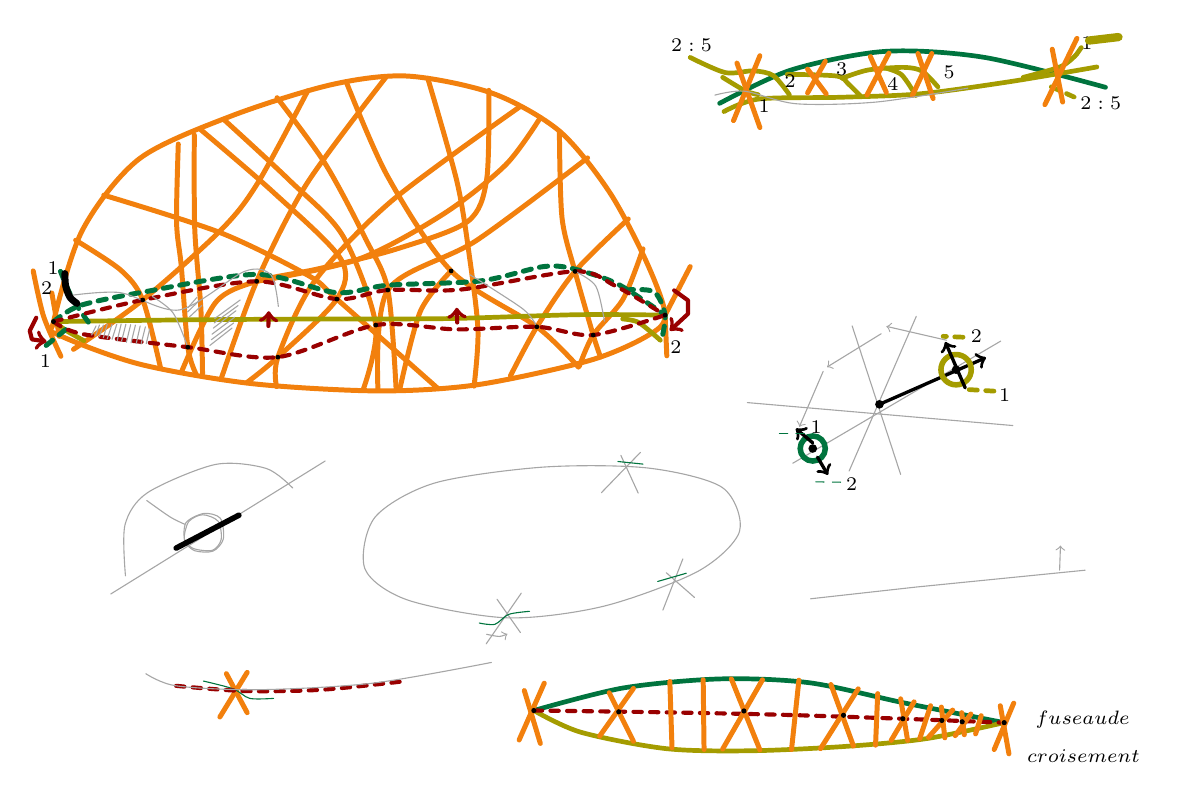
\begin{tikzpicture}[x=.55cm,y=-.55cm,line cap=round,line join=round,g/.style={olive!80!yellow,line width=1.7pt},r/.style={orange!80!brown,line width=1.8pt},w/.style={red!60!black,line width=1.5pt},b/.style={blue!60!black,line width=1.4pt},p/.style={gray!70,thin},k/.style={black,line width=1.2pt},every node/.style={font=\scriptsize}]
% Small upper-right strip and numbered sectors.
\draw[blue!35!green!70!black,line width=1.7pt] plot[smooth] coordinates {(17.87,2.74) (19.52,1.97) (21.69,1.54) (23.99,1.68) (26.78,2.37)};
\draw[g] plot[smooth] coordinates {(17.97,2.93) (18.78,2.64) (20.66,2.6) (22.5,2.52) (24.57,2.24) (26.58,1.9)};
\draw[g] plot[smooth] coordinates {(17.19,1.68) (18.0,2.03) (18.65,1.99) (19.11,2.1) (19.48,2.54)};
\draw[g] plot[smooth] coordinates {(17.94,2.14) (18.46,2.45) (18.76,2.54)};
\draw[g] plot[smooth] coordinates {(19.43,2.07) (20.57,2.11) (20.84,2.29) (21.13,2.58)};
\draw[g] plot[smooth] coordinates {(20.7,2.16) (21.3,1.97) (22.13,1.91) (22.55,2.0) (22.91,2.36)};
\draw[g] plot[smooth] coordinates {(21.68,1.92) (22.07,2.08) (22.4,2.56)};
\draw[g] plot[smooth] coordinates {(24.88,2.14) (25.75,1.89) (26.1,1.62)};
\draw[g,dashed] plot[smooth] coordinates {(25.53,2.36) (26.18,2.65)};
\draw[g,dashed] plot[smooth] coordinates {(26.11,1.61) (26.32,1.31)};
\draw[r] plot[smooth] coordinates {(18.27,1.81) (18.8,3.3)};
\draw[r] plot[smooth] coordinates {(18.8,1.64) (18.19,3.14)};
\draw[r] plot[smooth] coordinates {(19.9,1.95) (20.33,2.52)};
\draw[r] plot[smooth] coordinates {(20.31,1.77) (19.9,2.5)};
\draw[r] plot[smooth] coordinates {(21.35,1.66) (21.72,2.49)};
\draw[r] plot[smooth] coordinates {(21.78,1.58) (21.27,2.55)};
\draw[r] plot[smooth] coordinates {(22.45,1.59) (22.8,2.63)};
\draw[r] plot[smooth] coordinates {(22.77,1.59) (22.32,2.56)};
\draw[r] plot[smooth] coordinates {(25.55,1.49) (25.79,2.71)};
\draw[r] plot[smooth] coordinates {(26.12,1.24) (25.38,2.77)};
\draw[p] plot[smooth] coordinates {(17.76,2.55) (18.45,2.46) (19.64,2.75) (21.49,2.71) (23.6,2.39)};
\node at (17.22,1.39) {$2:5$};
\node at (18.9,2.8) {$1$};
\node at (19.5,2.24) {$2$};
\node at (20.69,1.95) {$3$};
\node at (21.87,2.29) {$4$};
\node at (23.17,2.02) {$5$};
\node at (26.35,1.35) {$1$};
\node at (26.67,2.73) {$2:5$};
\draw[g,line width=3pt] (26.4,1.29)--(27.08,1.21);
% Large orange bounded arrangement: all crossing curves and marked intersections.
\draw[r] plot[smooth cycle] coordinates {(2.49,7.78) (3.16,5.66) (4.47,4.02) (6.6,3.03) (8.9,2.31) (10.66,2.11) (12.63,2.51) (14.17,3.38) (15.32,4.78) (16.18,6.4) (16.61,7.63) (16.2,8.11) (14.86,8.68) (12.26,9.24) (9.97,9.38) (7.05,9.21) (4.47,8.76) (2.59,8.08)};
\draw[r] plot[smooth] coordinates {(3.0,5.9) (4.04,6.59) (4.55,7.28) (4.96,8.85)};
\draw[r] plot[smooth] coordinates {(3.65,4.86) (6.35,5.73) (8.38,6.72) (9.03,7.26) (11.36,9.32)};
\draw[r] plot[smooth] coordinates {(5.37,3.68) (5.33,5.49) (5.44,6.51) (5.59,8.37) (5.78,8.99)};
\draw[r] plot[smooth] coordinates {(5.74,3.47) (5.75,5.64) (5.89,7.46) (5.93,8.99)};
\draw[r] plot[smooth] coordinates {(5.89,3.35) (7.55,4.78) (9.12,6.33) (9.03,7.26) (7.67,8.6) (6.95,9.19)};
\draw[r] plot[smooth] coordinates {(6.44,3.13) (7.94,4.52) (9.17,5.8) (9.93,7.86) (9.64,9.35)};
\draw[r] plot[smooth] coordinates {(7.65,2.61) (8.76,4.13) (9.69,5.86) (10.21,7.05) (10.4,9.35)};
\draw[r] plot[smooth] coordinates {(8.36,2.45) (7.21,4.57) (6.37,5.65) (4.55,7.28) (2.95,8.42)};
\draw[r] plot[smooth] coordinates {(9.25,2.25) (10.2,4.42) (11.67,6.61) (13.65,7.9) (14.61,8.83)};
\draw[r] plot[smooth] coordinates {(10.17,2.13) (8.34,4.59) (7.18,6.85) (6.36,9.1)};
\draw[r] plot[smooth] coordinates {(11.13,2.16) (11.81,4.57) (12.1,6.33) (12.29,7.99) (12.2,9.27)};
\draw[r] plot[smooth] coordinates {(12.54,2.44) (12.49,4.5) (12.05,5.47) (10.42,6.1) (8.61,6.56) (7.18,6.85) (6.23,7.34) (5.44,8.95)};
\draw[r] plot[smooth] coordinates {(13.27,2.81) (10.3,4.99) (8.5,6.87) (7.67,8.6) (7.64,9.28)};
\draw[r] plot[smooth] coordinates {(13.73,3.07) (12.93,4.16) (11.5,5.29) (9.53,6.34) (7.18,6.85)};
\draw[r] plot[smooth] coordinates {(14.17,3.38) (14.23,5.38) (14.53,6.62) (14.95,8.09) (15.12,8.6)};
\draw[r] plot[smooth] coordinates {(14.82,4.0) (12.25,5.91) (10.21,7.05) (9.98,9.35)};
\draw[r] plot[smooth] coordinates {(15.76,5.41) (14.53,6.62) (13.65,7.9) (13.04,9.03)};
\draw[r] plot[smooth] coordinates {(16.1,6.1) (15.64,7.26) (14.95,8.09) (14.63,8.81)};
\draw[r] plot[smooth] coordinates {(11.67,6.61) (10.96,7.54) (10.48,9.36)};
\draw[r] plot[smooth] coordinates {(2.02,6.61) (2.26,7.66) (2.66,8.58)};
\draw[r] plot[smooth] coordinates {(2.45,7.12) (2.56,7.75) (2.62,8.12)};
\draw[r] plot[smooth] coordinates {(16.61,7.63) (17.19,6.51)};
\draw[r] plot[smooth] coordinates {(16.61,7.63) (16.65,8.57)};
\draw[g] plot[smooth] coordinates {(2.49,7.78) (5.53,7.74) (8.53,7.72) (11.6,7.71) (14.6,7.62) (16.61,7.63)};
\draw[g] plot[smooth] coordinates {(2.49,7.78) (2.82,8.01) (3.19,8.22)};
\draw[g] plot[smooth] coordinates {(15.63,7.72) (16.0,7.8) (16.5,8.21)};
\draw[blue!35!green!70!black,line width=1.8pt,dashed] plot[smooth] coordinates {(2.49,7.78) (3.1,7.41) (4.55,7.1) (7.18,6.69) (9.01,7.11) (10.21,6.94) (12.35,6.84) (13.8,6.51) (14.53,6.57) (15.53,6.92) (16.61,7.63)};
\draw[blue!35!green!70!black,line width=1.8pt,dashed] plot[smooth] coordinates {(2.65,6.62) (2.93,7.26) (3.35,7.87)};
\draw[blue!35!green!70!black,line width=1.8pt,dashed] plot[smooth] coordinates {(2.32,8.33) (2.87,7.88)};
\draw[blue!35!green!70!black,line width=1.8pt,dashed] plot[smooth] coordinates {(15.69,7.05) (16.35,7.09) (16.61,7.63) (16.52,8.24)};
\draw[w,dashed] plot[smooth] coordinates {(2.49,7.78) (4.55,7.28) (7.18,6.85) (9.03,7.26) (10.21,7.05) (11.89,7.04) (14.53,6.62) (15.47,6.96) (16.61,7.63)};
\draw[w,dashed] plot[smooth] coordinates {(2.49,7.78) (3.17,8.07) (5.59,8.37) (7.67,8.6) (9.93,7.86) (11.79,7.96) (13.65,7.9) (14.95,8.09) (16.61,7.63)};
\draw[p] plot[smooth] coordinates {(2.85,7.18) (4.02,7.11) (5.4,7.51) (6.9,6.62) (7.51,6.7) (7.68,7.43)};
\draw[p] plot[smooth] coordinates {(4.77,7.2) (5.25,7.58) (5.59,8.37)};
\draw[p] plot[smooth] coordinates {(12.11,6.7) (13.33,7.49) (13.65,7.9)};
\draw[p] plot[smooth] coordinates {(14.53,6.62) (15.01,6.96) (15.21,7.77)};
\draw[p] (3.47,7.88)--(3.37,8.09);
\draw[p] (3.55,7.86)--(3.46,8.1);
\draw[p] (3.64,7.86)--(3.55,8.12);
\draw[p] (3.73,7.84)--(3.64,8.15);
\draw[p] (3.84,7.84)--(3.73,8.18);
\draw[p] (3.95,7.84)--(3.84,8.19);
\draw[p] (4.05,7.84)--(3.96,8.22);
\draw[p] (4.16,7.84)--(4.06,8.23);
\draw[p] (4.27,7.85)--(4.17,8.26);
\draw[p] (4.38,7.86)--(4.28,8.27);
\draw[p] (4.49,7.88)--(4.4,8.28);
\draw[p] (4.61,7.9)--(4.51,8.3);
\draw[p] (4.71,7.95)--(4.63,8.29);
\draw[p] (5.59,7.46)--(5.8,7.22);
\draw[p] (5.58,7.56)--(5.86,7.29);
\draw[p] (5.63,7.67)--(5.91,7.41);
\draw[p] (6.21,7.71)--(6.8,7.28);
\draw[p] (6.2,7.81)--(6.75,7.41);
\draw[p] (6.18,7.93)--(6.7,7.53);
\draw[p] (6.15,8.07)--(6.67,7.68);
\draw[p] (6.13,8.2)--(6.65,7.81);
\draw[p] (6.1,8.33)--(6.61,7.93);
\draw[k,line width=2.5pt] plot[smooth] coordinates {(2.75,6.67) (2.77,6.96) (2.87,7.22) (3.03,7.36)};
\draw[w,->] (2.09,7.69)--(1.94,7.99)--(1.99,8.19)--(2.33,8.24);
\draw[w,->] (16.82,7.06)--(17.14,7.29)--(17.14,7.6)--(16.72,7.99);
\draw[w,->] (7.45,7.88)--(7.46,7.54);
\draw[w,->] (11.81,7.8)--(11.8,7.46);
\fill[black] (2.49,7.78) circle (.055);
\fill[black] (4.55,7.28) circle (.055);
\fill[black] (5.59,8.37) circle (.055);
\fill[black] (7.18,6.85) circle (.055);
\fill[black] (7.67,8.6) circle (.055);
\fill[black] (9.03,7.26) circle (.055);
\fill[black] (9.93,7.86) circle (.055);
\fill[black] (10.21,7.05) circle (.055);
\fill[black] (11.67,6.61) circle (.055);
\fill[black] (13.65,7.9) circle (.055);
\fill[black] (14.53,6.62) circle (.055);
\fill[black] (14.95,8.09) circle (.055);
\fill[black] (16.61,7.63) circle (.055);
\node at (2.3,8.69) {$1$};
\node at (2.33,7.01) {$2$};
\node at (2.48,6.54) {$1$};
\node at (16.86,8.38) {$2$};
% Middle-right oriented radial drawing with two coloured circled points.
\draw[p] (20.93,7.88)--(22.05,11.31);
\draw[p] (22.41,7.66)--(20.86,11.23);
\draw[p] (18.51,9.65)--(24.64,10.18);
\draw[p] (19.56,11.05)--(24.36,8.23);
\draw[p,->] (21.6,8.06)--(20.35,8.83);
\draw[p,->] (20.26,8.93)--(19.71,10.21);
\draw[p,->] (23.11,8.21)--(21.72,7.89);
\draw[k,->] (21.56,9.69)--(24.02,8.61);
\draw[g,line width=2pt] (23.33,8.89) circle (.35);
\draw[blue!35!green!70!black,line width=2pt] (20.02,10.71) circle (.29);
\draw[k,->] (23.54,9.31)--(23.08,8.25);
\draw[k,->] (20.13,10.91)--(20.37,11.32);
\draw[k,->] (20.02,10.58)--(19.63,10.25);
\fill[black] (21.56,9.69) circle (.1);
\fill[black] (23.33,8.89) circle (.1);
\fill[black] (20.02,10.71) circle (.1);
\draw[g,dashed] plot[smooth] coordinates {(23.49,8.14) (23.03,8.12)};
\draw[g,dashed] plot[smooth] coordinates {(23.63,9.35) (24.28,9.39)};
\draw[blue!35!green!70!black,dashed] plot[smooth] coordinates {(19.25,10.36) (19.88,10.36)};
\draw[blue!35!green!70!black,dashed] plot[smooth] coordinates {(20.09,11.48) (20.79,11.49)};
\node at (23.8,8.11) {$2$};
\node at (24.45,9.47) {$1$};
\node at (20.1,10.21) {$1$};
\node at (20.92,11.53) {$2$};
% Faint left circular construction and central oval with local crossings.
\draw[p] plot[smooth] coordinates {(3.81,14.07) (8.76,11.0)};
\draw[p] plot[smooth] coordinates {(4.15,13.65) (4.14,12.47) (4.66,11.73) (6.22,11.08) (7.4,11.17) (8.01,11.62)};
\draw[p] plot[smooth cycle] coordinates {(5.96,12.21) (6.34,12.32) (6.41,12.8) (6.17,13.08) (5.75,13.07) (5.52,12.84) (5.55,12.42)};
\draw[p] plot[smooth cycle] coordinates {(5.93,12.24) (6.29,12.39) (6.36,12.81) (6.16,13.06) (5.72,13.02) (5.51,12.8) (5.61,12.4)};
\draw[k,line width=2pt] (5.32,13.01)--(6.77,12.25);
\draw[p] plot[smooth] coordinates {(4.64,11.91) (5.18,12.29) (5.52,12.46)};
\fill[black] (5.98,12.68) circle (.045);
\draw[p] plot[smooth cycle] coordinates {(13.79,11.14) (16.21,11.16) (17.93,11.61) (18.33,12.62) (17.38,13.54) (15.2,14.35) (12.97,14.62) (10.67,14.21) (9.68,13.49) (9.91,12.3) (11.28,11.51)};
\draw[p] (15.59,10.87)--(15.99,11.74);
\draw[p] (16.04,10.8)--(15.14,11.73);
\draw[p] (16.64,13.58)--(17.29,14.15);
\draw[p] (17.02,13.26)--(16.56,14.44);
\draw[p] (12.73,14.19)--(13.27,14.96);
\draw[p] (13.29,14.05)--(12.48,15.22);
\draw[blue!35!green!70!black] plot[smooth] coordinates {(15.52,11.01) (16.1,11.07)};
\draw[blue!35!green!70!black] plot[smooth] coordinates {(16.44,13.78) (17.1,13.59)};
\draw[blue!35!green!70!black] plot[smooth] coordinates {(12.32,14.74) (12.68,14.77) (13.0,14.54) (13.48,14.47)};
\draw[p,->] plot[smooth] coordinates {(12.49,15.0) (12.78,15.05) (12.97,14.99)};
\draw[p] (19.97,14.18)--(22.4,13.91)--(26.31,13.52);
\draw[p,->] (25.72,13.52)--(25.74,12.95);
% Short lower-left dashed curve through an orange crossing.
\draw[r] (6.48,15.91)--(6.96,16.81);
\draw[r] (6.96,15.88)--(6.33,16.91);
\draw[blue!35!green!70!black] plot[smooth] coordinates {(5.95,16.08) (6.64,16.26) (7.02,16.48) (7.57,16.48)};
\draw[w,dashed] plot[smooth] coordinates {(5.32,16.19) (6.9,16.31) (8.68,16.28) (10.62,16.08)};
\draw[p] plot[smooth] coordinates {(4.62,15.91) (5.32,16.19) (7.2,16.28) (9.85,16.13) (12.6,15.65)};
% Lower fuseau de croisement.
\draw[blue!35!green!70!black,line width=1.7pt] plot[smooth] coordinates {(13.58,16.76) (15.64,16.24) (17.89,16.03) (19.95,16.12) (22.11,16.58) (24.44,17.04)};
\draw[g] plot[smooth] coordinates {(13.58,16.76) (14.66,17.26) (16.63,17.64) (18.57,17.69) (20.76,17.59) (22.64,17.41) (24.44,17.04)};
\draw[w,dashed] plot[smooth] coordinates {(13.58,16.76) (16.5,16.8) (19.36,16.86) (22.07,16.95) (24.44,17.04)};
\draw[r] plot[smooth] coordinates {(13.36,16.3) (13.73,17.52)};
\draw[r] plot[smooth] coordinates {(13.82,16.13) (13.24,17.44)};
\draw[r] plot[smooth] coordinates {(15.32,16.35) (15.88,17.47)};
\draw[r] plot[smooth] coordinates {(15.88,16.25) (15.1,17.35)};
\draw[r] plot[smooth] coordinates {(16.72,16.09) (16.77,17.62)};
\draw[r] plot[smooth] coordinates {(17.49,16.05) (17.51,17.66)};
\draw[r] plot[smooth] coordinates {(18.14,16.03) (18.8,17.67)};
\draw[r] plot[smooth] coordinates {(18.86,16.05) (17.94,17.65)};
\draw[r] plot[smooth] coordinates {(19.7,16.06) (19.53,17.66)};
\draw[r] plot[smooth] coordinates {(20.44,16.16) (20.96,17.58)};
\draw[r] plot[smooth] coordinates {(21.07,16.26) (20.2,17.64)};
\draw[r] plot[smooth] coordinates {(21.52,16.37) (21.47,17.56)};
\draw[r] plot[smooth] coordinates {(22.05,16.49) (22.21,17.45)};
\draw[r] plot[smooth] coordinates {(22.36,16.56) (21.83,17.45)};
\draw[r] plot[smooth] coordinates {(22.74,16.65) (22.49,17.41)};
\draw[r] plot[smooth] coordinates {(22.99,16.68) (23.07,17.39)};
\draw[r] plot[smooth] coordinates {(23.25,16.75) (22.69,17.38)};
\draw[r] plot[smooth] coordinates {(23.46,16.81) (23.52,17.32)};
\draw[r] plot[smooth] coordinates {(23.67,16.84) (23.31,17.34)};
\draw[r] plot[smooth] coordinates {(23.91,16.88) (23.78,17.3)};
\draw[r] plot[smooth] coordinates {(24.35,16.65) (24.55,17.76)};
\draw[r] plot[smooth] coordinates {(24.66,16.59) (24.21,17.66)};
\fill[black] (13.58,16.76) circle (.06);
\fill[black] (15.54,16.79) circle (.06);
\fill[black] (18.43,16.77) circle (.06);
\fill[black] (20.73,16.87) circle (.06);
\fill[black] (22.1,16.95) circle (.06);
\fill[black] (23.0,16.99) circle (.06);
\fill[black] (23.47,17.02) circle (.06);
\fill[black] (24.44,17.04) circle (.06);
\node at (26.25,16.96) {$\text{fuseau de}$};
\node at (26.27,17.81) {$\text{croisement}$};
\end{tikzpicture}}
\[\sigma_2=\text{\unsure{chang\textsuperscript{t}} de \uline{l'orientation} de }D\]
\[\text{et}\]
\[\sigma_0=\ ?\]

les repères de la surface correspondent aux p.r. \inserted{\uline{$\unsure{\overrightarrow D}$ orientées}} qui \deleted{\unsure{sont}\ \unsure{principales}} \inserted{sont} de \unsure{tricalité|criticalité} $\geq2$, \uline{munis} de plus d'un sommet $s$ et d'une orientation en ce sommet i.e. d'une rive du complémentaire $D\setminus\{s\}$.
\margin{\mspage{137}}

\scanpage{139}
\[\sigma_1\quad\sigma\quad\sigma_2\quad\sigma_0\]
\diagram{\[\begin{tikzcd}[ampersand replacement=\&,column sep=large,row sep=large,arrows={line width=1.5pt},g/.style={olive!80!yellow},r/.style={orange!80!brown}]
\&\&\&\overset{\sigma_1\sigma_0}{\bullet}\arrow[d,g]\&\&\\
\&\&\&\underset{(\sigma_1,\sigma_0)}{\bullet}\&\&\\
\&\&\overset{\sigma_1\sigma_2}{\bullet}\arrow[d,g]\&\&\&\\
\&\underset{\sigma_1}{\bullet}\arrow[r,g]\arrow[d,r]\arrow[uurr,g,out=90,in=180,looseness=1.5]\&\overset{(\sigma_1,\sigma_2)}{\bullet}\&\overset{\sigma_2}{\bullet}\arrow[l,g]\arrow[dl,r]\arrow[dr,r]\&\&\\
\underset{\sigma_1\sigma}{\bullet}\arrow[r,r]\&\underset{(\sigma_1,\sigma)}{\bullet}\arrow[ur,g]\&\underset{(\sigma,\sigma_2)}{\bullet}\arrow[u,r]\arrow[dr,r]\&\&\underset{(\sigma_2,\sigma_0)}{\bullet}\arrow[dl,g]\&\underset{\sigma_0\sigma_2}{\bullet}\arrow[l,r,dashed]\\
\&\underset{\sigma}{\bullet}\arrow[u,r]\arrow[ur,r]\arrow[rr,g]\&\&\underset{(\sigma,\sigma_0)}{\bullet}\&\underset{\sigma_0}{\bullet}\arrow[u,r]\arrow[l,g]\arrow[uuuul,g,out=85,in=0,looseness=1.8]\&\\
\&\&\underset{\sigma\sigma_2}{\bullet}\arrow[uu,r,densely dotted]\&\underset{\sigma\sigma_0}{\bullet}\arrow[u,g]\&\&
\end{tikzcd}\]}
\figure{\begin{tikzpicture}[x=.55cm,y=-.55cm]\draw[black,thin] (21.17,2.98)--(21.36,2.83);\end{tikzpicture}}
\margin{\mspage{138}}

\scanpage{140}
\unsure{1} sommet\\
1 face\\
2 arêtes\\
\unsure{4} repères, correspondent\\
aux rives des arêtes $a,b$

\deleted{$\sigma_0,\ \unsure{\sigma_1}\ \unsure{\hat a}$}

$\sigma_0=\sigma_2$ échangent $a^+,a^-$ et $b^+,b^-$\\
$\sigma_1$ échange \deleted{$\unsure{a^+\text{ et }a^-}$} $a^+$ et $b^+$, $a^-$ et $b^-$\\
$\sigma$ échange $a^+$ et $b^-$, $b^+$ et $a^-$

\[\underbrace{\sigma_1,\sigma},\underbrace{\sigma_2,\sigma_0}_{\substack{\Vert\\\sigma'}}\]
subdivision barycentrique

$\sigma_0=\sigma_2$ soit $\sigma'$, commute à $\sigma$\\
$\sigma_1=\sigma\sigma'$,\\
\deleted{$\unsure{\sigma=\sigma_1\sigma'}$}

\[\underbrace{\sigma\sigma'}_{\sigma_1},\underbrace{\sigma}_{\sigma},
\underbrace{\underbrace{\sigma'}_{\sigma_2},\underbrace{\sigma'}_{\sigma_0}}\]
\[\underbrace{\sigma\sigma'}_{\sigma'_0},\underbrace{\sigma'}_{\sigma'_1},\underbrace{\sigma}_{\sigma'_2}\]
\figure{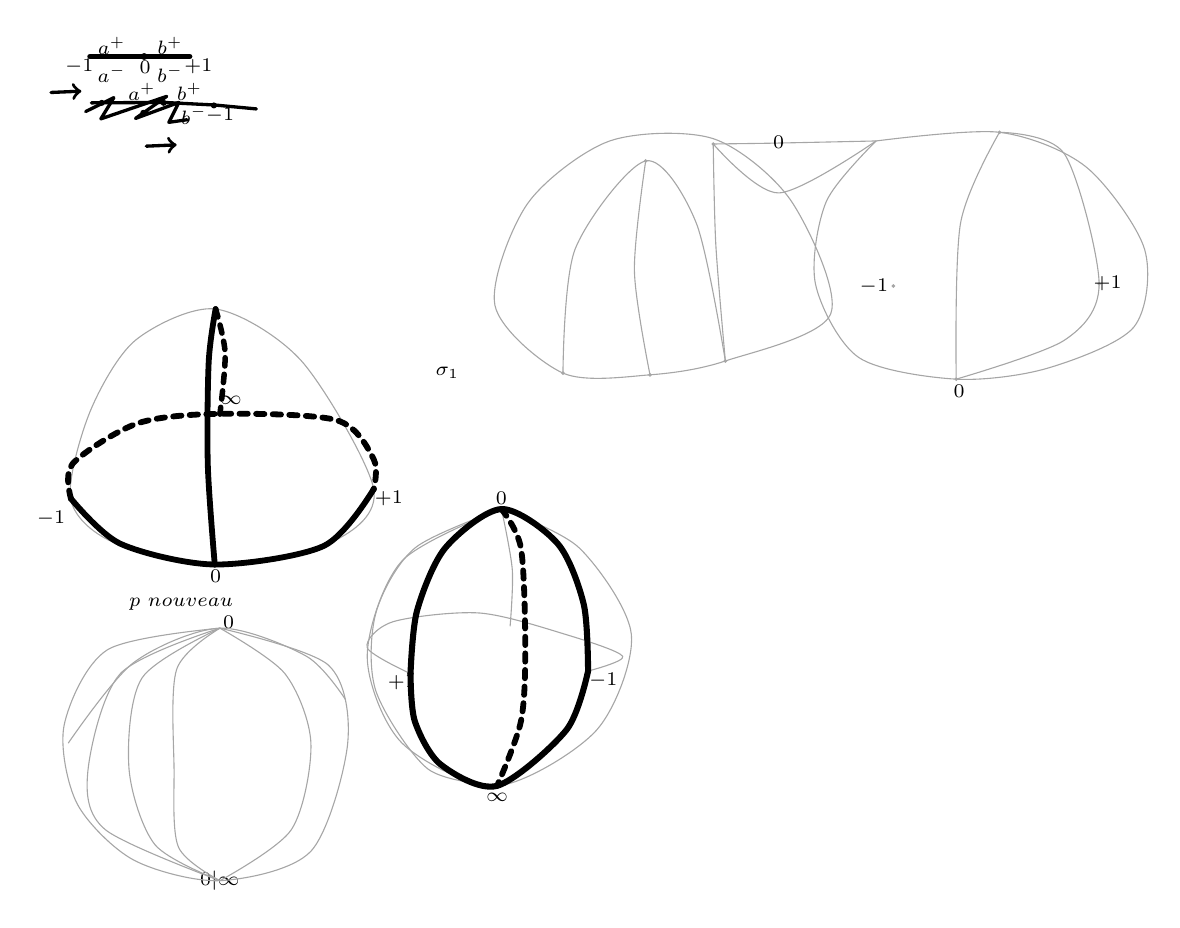
\begin{tikzpicture}[x=.55cm,y=-.55cm,line cap=round,line join=round,g/.style={olive!80!yellow,line width=1.7pt},r/.style={orange!80!brown,line width=1.8pt},w/.style={red!60!black,line width=1.5pt},b/.style={blue!60!black,line width=1.4pt},p/.style={gray!70,thin},k/.style={black,line width=1.2pt},every node/.style={font=\scriptsize}]
% Upper-left segments and overdrawn segment.
\draw[k,line width=2pt] (3.0,1.15)--(5.3,1.15);
\fill[k] (4.25,1.15) circle (.08);
\node at (2.75,1.37) {$-1$};
\node at (5.5,1.37) {$+1$};
\node at (4.27,1.4) {$0$};
\node at (3.5,.9) {$a^+$};
\node at (4.85,.9) {$b^+$};
\node at (3.5,1.55) {$a^-$};
\node at (4.85,1.55) {$b^-$};
\deleted{\begin{scope}
\draw[k] (3.03,2.22)--(4.7,2.21)--(5.88,2.27)--(6.84,2.36);
\draw[k] (2.9,2.42)--(3.55,2.1)--(3.25,2.59)--(4.77,2.07)--(4.05,2.58)--(5.05,2.21)--(4.82,2.67)--(5.24,2.61);
\fill[k] (3.27,2.22) circle (.07);
\fill[k] (4.7,2.22) circle (.07);
\fill[k] (4.23,2.45) circle (.07);
\fill[k] (5.86,2.28) circle (.07);
\node at (4.2,1.97) {$a^+$};
\node at (5.3,1.97) {$b^+$};
\node at (5.4,2.51) {$b^-$};
\node at (6,2.5) {$\unsure{-1}$};
\end{scope}}
\draw[k,->] (2.1,1.98)--(2.8,1.95);
\draw[k,->] (4.3,3.22)--(5.0,3.19);
% Upper pencil globes.
\draw[p] plot[smooth cycle] coordinates {(12.35,6.9) (13.1,4.55) (15.0,3.1) (17.4,3.05) (19.2,4.5) (20.1,7.1) (17.67,8.18) (15.93,8.5) (13.92,8.46)};
\draw[p] plot[smooth] coordinates {(13.92,8.46) (14.2,5.6) (15.83,3.56) (17.0,5.0) (17.67,8.18)};
\draw[p] plot[smooth] coordinates {(15.83,3.56) (15.57,6.1) (15.93,8.5)};
\draw[p] plot[smooth] coordinates {(17.39,3.17) (17.45,5.5) (17.67,8.18)};
\draw[p] plot[smooth] coordinates {(17.39,3.17) (18.8,3.15) (21.15,3.1)};
\draw[p] plot[smooth] coordinates {(17.39,3.17) (18.9,4.3) (21.15,3.1)};
\draw[p] plot[smooth] coordinates {(21.15,3.1) (20.0,4.5) (19.75,6.4) (20.75,8.1) (23.0,8.6) (25.1,8.35) (27.1,7.4) (27.35,5.6) (26.0,3.7) (24.0,2.9) (21.15,3.1)};
\draw[p] plot[smooth] coordinates {(24.0,2.9) (23.1,5.0) (23.0,8.6)};
\draw[p] plot[smooth] coordinates {(24.0,2.9) (25.5,3.4) (26.3,6.4) (25.5,7.7) (23.0,8.6)};
\fill[p] (13.92,8.46) circle (.045);
\fill[p] (15.83,3.56) circle (.045);
\fill[p] (15.93,8.5) circle (.045);
\fill[p] (17.39,3.17) circle (.045);
\fill[p] (17.67,8.18) circle (.045);
\fill[p] (21.55,6.45) circle (.045);
\fill[p] (24.0,2.9) circle (.045);
\fill[p] (26.3,6.4) circle (.045);
\fill[p] (23.0,8.6) circle (.045);
\node at (18.9,3.12) {$\unsure{0}$};
\node at (11.25,8.45) {$\sigma_1$};
\node at (21.1,6.45) {$-1$};
\node at (26.5,6.4) {$+1$};
\node at (23.07,8.88) {$0$};
% Large left ink ellipse with pencil construction.
\draw[p] plot[smooth cycle] coordinates {(2.55,11.35) (3.0,9.35) (4.05,7.7) (5.9,6.98) (7.9,8.2) (9.55,11.14) (8.6,12.35) (5.88,12.88) (3.5,12.35)};
\draw[k,line width=2.1pt] plot[smooth] coordinates {(2.56,11.36) (3.7,12.4) (5.88,12.88) (8.4,12.45) (9.55,11.14)};
\draw[k,line width=2.1pt,dashed] plot[smooth] coordinates {(2.56,11.36) (2.6,10.55) (4.1,9.62) (6.0,9.4) (8.7,9.55) (9.55,10.45) (9.55,11.14)};
\draw[k,line width=2.1pt] plot[smooth] coordinates {(5.9,6.98) (5.74,8.2) (5.72,10.6) (5.88,12.88)};
\draw[k,line width=2pt,dashed] plot[smooth] coordinates {(5.9,6.98) (6.12,8.0) (6.0,9.4)};
\fill[k] (2.56,11.36) circle (.07);
\fill[k] (9.55,11.14) circle (.07);
\fill[k] (5.88,12.88) circle (.07);
\fill[k] (6.0,9.4) circle (.07);
\node at (2.1,11.82) {$-1$};
\node at (9.9,11.35) {$+1$};
\node at (5.9,13.15) {$0$};
\node at (6.25,9.1) {$\infty$};
% Faint lower-left globe.
\node at (5.1,13.8) {$\unsure{p\ \text{nouveau}}$};
\node at (6.2,14.22) {$0$};
\node at (6.0,20.18) {$\unsure{0|\infty}$};
\draw[p] plot[smooth] coordinates {(6.0,14.35) (3.4,14.85) (2.4,16.6) (2.7,18.4) (4.0,19.7) (6.0,20.18) (8.1,19.5) (8.95,17.0) (8.5,15.2) (6.0,14.35)};
\draw[p] plot[smooth] coordinates {(6.0,14.35) (5.0,15.3) (4.94,17.6) (5.04,19.4) (6.0,20.18)};
\draw[p] plot[smooth] coordinates {(6.0,14.35) (4.2,15.5) (3.9,17.6) (4.5,19.35) (6.0,20.18)};
\draw[p] plot[smooth] coordinates {(6.0,14.35) (3.7,15.4) (2.95,17.65) (3.35,19.0) (6.0,20.18)};
\draw[p] plot[smooth] coordinates {(6.0,14.35) (7.5,15.4) (8.1,17.0) (7.65,19.0) (6.0,20.18)};
\draw[p] plot[smooth] coordinates {(2.5,17.0) (4.0,15.15) (6.0,14.35) (8.0,15.0) (8.9,16.0)};
% Lower central oval with dashed meridian and faint surrounding constructions.
\draw[p] plot[smooth] coordinates {(12.5,11.6) (10.2,12.8) (9.4,15.0) (10.2,17.0) (12.4,17.99) (14.7,16.7) (15.5,14.5) (14.3,12.5) (12.5,11.6)};
\draw[p] plot[smooth] coordinates {(12.5,11.6) (10.5,12.5) (9.6,14.0) (9.6,15.8) (10.8,17.6) (12.4,17.99)};
\draw[p] plot[smooth] coordinates {(10.4,15.4) (9.4,14.8) (10.0,14.2) (12.0,14.0) (14.0,14.5) (15.3,15.0) (14.5,15.34)};
\draw[p] plot[smooth] coordinates {(12.5,11.6) (12.75,13.0) (12.7,14.3)};
\draw[k,line width=2.2pt] plot[smooth] coordinates {(10.4,15.4) (10.55,13.95) (11.2,12.5) (12.5,11.6) (13.8,12.4) (14.4,13.8) (14.5,15.34)};
\draw[k,line width=2.2pt] plot[smooth] coordinates {(14.5,15.34) (14.0,16.7) (12.4,17.99) (11.1,17.5) (10.5,16.5) (10.4,15.4)};
\draw[k,line width=2.1pt,dashed] plot[smooth] coordinates {(12.5,11.6) (12.95,12.5) (13.05,14.8) (12.95,16.5) (12.4,17.99)};
\fill[k] (10.4,15.4) circle (.065);
\fill[k] (14.5,15.34) circle (.065);
\fill[k] (12.4,17.99) circle (.065);
\node at (12.5,11.35) {$0$};
\node at (12.4,18.25) {$\infty$};
\node at (10.2,15.6) {$\unsure{+1}$};
\node at (14.85,15.55) {$-1$};
\end{tikzpicture}}
\margin{\mspage{139}}

\scanpage{141}
\figure{\begin{tikzpicture}[x=.55cm,y=-.55cm,line cap=round,line join=round,g/.style={olive!80!yellow,line width=1.7pt},r/.style={orange!80!brown,line width=1.8pt},w/.style={red!60!black,line width=1.5pt},b/.style={blue!60!black,line width=1.4pt},p/.style={gray!70,thin},k/.style={black,line width=1.2pt},every node/.style={font=\scriptsize}]
% Main arrangement: continuous construction curves, numbered moving lines, hatching and overwritten strokes.
\draw[p,line width=.9pt] plot[smooth] coordinates {(2.15,5.3) (3.7,5.65) (7.0,6.55) (11.23,7.9) (15.2,9.2) (21.95,11.6)};
\draw[p,line width=.9pt] plot[smooth] coordinates {(19.5,1.05) (16.4,3.4) (13.78,6.18) (10.3,7.6) (7.8,9.2) (6.0,11.63) (5.35,14.85) (5.4,18.2) (4.9,20.65)};
\draw[p,line width=.9pt] plot[smooth] coordinates {(12.2,.15) (12.47,1.4) (12.73,1.92) (14.0,3.3) (15.2,4.84) (15.38,6.62) (14.6,9.5) (12.6,13.2) (10.14,15.2) (8.7,16.5) (7.25,19.1) (7.5,21.8)};
\draw[p,line width=.9pt] plot[smooth] coordinates {(14.15,.2) (12.73,1.92) (9.74,5.45) (8.2,7.4) (6.8,9.65) (6.0,11.63) (6.6,13.3) (6.2,16.9) (5.85,18.65) (5.55,20.6)};
\draw[p,line width=.9pt] plot[smooth] coordinates {(13.2,.2) (12.47,1.4) (9.6,3.68) (7.1,5.8) (5.9,8.0) (5.55,10.18) (6.0,11.63) (6.22,12.2) (6.6,13.3) (6.95,16.4) (6.2,21.1)};
\draw[k] (9.2,.18)--(9.6,3.68)--(9.74,5.45)--(9.85,7.45)--(9.9,8.42)--(10.0,10.04)--(10.11,12.38)--(10.14,15.2)--(9.7,21.92);
\draw[k] (4.3,3.9)--(8.1,9.16)--(8.25,9.47)--(9.14,10.9)--(10.11,12.38)--(13.38,16.7);
\draw[k] (1.05,12.54)--(5.55,10.18)--(6.8,9.65)--(8.1,9.16)--(8.57,8.98)--(9.9,8.42)--(11.23,7.9)--(12.5,7.45)--(15.38,6.62)--(20.1,5.65)--(23.68,5.15);
\draw[k,dashed] plot[smooth] coordinates {(1.25,12.63) (5.55,10.28) (8.1,9.28) (9.9,8.42) (12.5,7.15) (16.0,6.15) (21.2,5.35)};
\draw[k,dashed] plot[smooth] coordinates {(1.4,14.6) (6.0,11.63) (8.25,9.47) (9.9,8.42) (13.78,6.18) (18.3,5.15) (21.0,4.8)};
\draw[k,dashed] plot[smooth] coordinates {(1.7,15.25) (6.22,12.2) (8.25,9.47) (9.9,8.42) (13.78,6.18) (18.3,4.75) (21.8,4.1)};
\draw[k,dashed] plot[smooth] coordinates {(1.1,16.2) (5.78,12.65) (8.25,9.47) (9.9,8.42) (13.78,6.18) (17.7,4.2) (23.3,3.6)};
\draw[k,dashed] plot[smooth] coordinates {(1.7,17.2) (6.2,13.1) (9.14,10.9) (9.9,8.42) (13.78,6.18) (15.32,5.55) (18.3,3.8) (20.1,2.95)};
\draw[k,dashed] plot[smooth] coordinates {(1.2,18.0) (6.2,13.2) (9.14,10.9) (9.9,8.42) (13.78,6.18) (15.2,4.84) (19.8,2.55)};
\draw[k,dashed] plot[smooth] coordinates {(1.6,18.5) (6.4,13.2) (9.14,10.9) (9.9,8.42) (10.35,7.6) (15.2,4.84) (19.1,2.3)};
\draw[k,dashed] plot[smooth] coordinates {(2.2,19.05) (5.35,14.85) (6.6,13.3) (9.14,10.9) (9.9,8.42) (10.35,7.6) (15.2,4.84) (18.9,1.3)};
\draw[k,dashed] plot[smooth] coordinates {(5.55,20.6) (6.2,16.9) (6.6,13.3) (9.9,8.42) (10.35,7.6) (12.73,1.92) (13.8,.2)};
\draw[k,dashed] plot[smooth] coordinates {(6.6,21.1) (7.4,16.7) (9.14,10.9) (9.9,8.42) (10.35,7.6) (12.47,1.4) (12.9,.45)};
\draw[k,line width=2.8pt] plot[smooth] coordinates {(5.78,12.65) (6.22,12.2)};
\draw[k,line width=2.8pt] plot[smooth] coordinates {(5.35,14.85) (6.6,13.3)};
\draw[k,line width=2.8pt] plot[smooth] coordinates {(6.6,13.3) (9.14,10.9)};
\draw[k,line width=2.8pt] plot[smooth] coordinates {(9.9,8.42) (10.35,7.6)};
\draw[k,line width=2.8pt] plot[smooth] coordinates {(13.78,6.18) (15.32,5.55)};
\draw[k,line width=2.8pt] plot[smooth] coordinates {(13.78,6.18) (15.2,4.84)};
\draw[k,line width=2.8pt] plot[smooth] coordinates {(10.0,10.04) (10.11,12.38)};
\draw[k,line width=2pt] plot[smooth] coordinates {(9.85,7.98) (10.35,7.6)};
\draw[k,line width=2pt] plot[smooth] coordinates {(13.65,6.25) (14.35,5.85) (15.24,5.51)};
\draw[k,line width=2pt] plot[smooth] coordinates {(13.65,6.25) (14.35,5.45) (15.24,4.86)};
\fill[k] (5.55,10.18) circle (.065);
\fill[k] (6.8,9.65) circle (.065);
\fill[k] (8.1,9.16) circle (.065);
\fill[k] (8.57,8.98) circle (.065);
\fill[k] (9.9,8.42) circle (.065);
\fill[k] (11.23,7.9) circle (.065);
\fill[k] (12.5,7.45) circle (.065);
\fill[k] (15.38,6.62) circle (.065);
\fill[k] (9.85,7.45) circle (.065);
\fill[k] (9.85,7.98) circle (.065);
\fill[k] (10.35,7.6) circle (.065);
\fill[k] (9.74,5.45) circle (.065);
\fill[k] (9.6,3.68) circle (.065);
\fill[k] (12.47,1.4) circle (.065);
\fill[k] (12.73,1.92) circle (.065);
\fill[k] (13.78,6.18) circle (.065);
\fill[k] (15.32,5.55) circle (.065);
\fill[k] (15.2,4.84) circle (.065);
\fill[k] (6.0,11.63) circle (.065);
\fill[k] (6.22,12.2) circle (.065);
\fill[k] (5.78,12.65) circle (.065);
\fill[k] (8.25,9.47) circle (.065);
\fill[k] (10.0,10.04) circle (.065);
\fill[k] (9.14,10.9) circle (.065);
\fill[k] (10.11,12.38) circle (.065);
\fill[k] (6.6,13.3) circle (.065);
\fill[k] (5.35,14.85) circle (.065);
\fill[k] (10.14,15.2) circle (.065);
\node at (3.5,5.55) {$A$};
\node at (4.3,3.82) {$F$};
\node at (13.6,16.6) {$F$};
\node at (19.85,.85) {$B$};
\node at (20.85,2.95) {$G$};
\node at (1.7,16.45) {$G$};
\node at (2.8,17.55) {$\unsure{B}$};
\node at (4.6,20.8) {$E$};
\node at (6.0,21.6) {$D$};
\node at (7.6,21.55) {$\unsure{C}$};
\node at (11.85,.4) {$\unsure{C}$};
\node at (13.2,.4) {$D$};
\node at (14.3,.4) {$E$};
\node at (5.2,10.05) {$d_1$};
\node at (6.62,9.42) {$e_1$};
\node at (8.02,8.88) {$f_1$};
\node at (8.65,8.73) {$g_1$};
\node at (10.15,8.6) {$\unsure{o}$};
\node at (11.25,8.18) {$a_0$};
\node at (12.7,7.7) {$b_1$};
\node at (15.7,6.85) {$c_1$};
\node at (9.5,7.32) {$b_{11}$};
\node at (9.55,7.96) {$a_{11}$};
\node at (10.45,7.3) {$a_7$};
\node at (11.9,6.15) {$a_8=a_9=a_{10}$};
\node at (13.0,5.5) {$\deleted{\unsure{a_{10}}}$};
\node at (9.3,5.4) {$c_{11}$};
\node at (9.3,3.65) {$d_{11}$};
\node at (11.85,1.55) {$b_{-1}=$};
\node at (12.7,1.0) {$b_{10}$};
\node at (12.8,2.4) {$b_9$};
\node at (13.65,5.95) {$a_6$};
\node at (15.1,5.53) {$\unsure{a_5}$};
\node at (14.9,4.65) {$\unsure{b_7}$};
\node at (6.2,11.2) {$\unsure{a_2}$};
\node at (5.62,11.6) {$\deleted{\unsure{a_2}}$};
\node at (6.4,12.02) {$\unsure{a_3}$};
\node at (5.95,12.8) {$a_4$};
\node at (8.55,9.55) {$\unsure{b_2|f_2}$};
\node at (10.35,10.2) {$g_{11}$};
\node at (9.45,10.9) {$c_{10}$};
\node at (9.55,11.3) {$\deleted{\unsure{c_{11}}}$};
\node at (10.45,12.4) {$f_{11}$};
\node at (6.95,13.45) {$c_9$};
\node at (5.72,15.0) {$b_8$};
\node at (10.45,15.42) {$e_{11}$};
\node[draw,ellipse,inner sep=1pt] at (1.0,12.18) {$1$};
\node[draw,ellipse,inner sep=1pt] at (1.0,12.85) {$1$};
\node[draw,ellipse,inner sep=1pt] at (1.4,14.35) {$2$};
\node[draw,ellipse,inner sep=1pt] at (1.6,14.95) {$3$};
\node[draw,ellipse,inner sep=1pt] at (1.75,15.5) {$4$};
\node[draw,ellipse,inner sep=1pt] at (1.8,17.15) {$5$};
\node[draw,ellipse,inner sep=1pt] at (1.0,18.05) {$6$};
\node[draw,ellipse,inner sep=1pt] at (1.4,18.55) {$7$};
\node[draw,ellipse,inner sep=1pt] at (1.85,19.5) {$8$};
\node[draw,ellipse,inner sep=1pt] at (5.35,20.95) {$9$};
\node[draw,ellipse,inner sep=1pt] at (6.8,21.25) {$10$};
\node[draw,ellipse,inner sep=1pt] at (10.0,21.8) {$11$};
\node[draw,ellipse,inner sep=1pt] at (8.8,.4) {$11$};
\node[draw,ellipse,inner sep=1pt] at (12.8,.3) {$10$};
\node[draw,ellipse,inner sep=1pt] at (13.75,.3) {$9$};
\node[draw,ellipse,inner sep=1pt] at (19.0,.95) {$8$};
\node[draw,ellipse,inner sep=1pt] at (19.5,1.95) {$7$};
\node[draw,ellipse,inner sep=1pt] at (20.0,2.25) {$6$};
\node[draw,ellipse,inner sep=1pt] at (20.4,2.75) {$5$};
\node[draw,ellipse,inner sep=1pt] at (23.6,3.55) {$4$};
\node[draw,ellipse,inner sep=1pt] at (21.95,4.15) {$3$};
\node[draw,ellipse,inner sep=1pt] at (21.0,4.8) {$2$};
\node[draw,ellipse,inner sep=1pt] at (19.7,5.4) {$\unsure{1}$};
\node[draw,ellipse,inner sep=1pt] at (21.3,5.5) {$1$};
\node at (2.95,11.4) {$\unsure{A}$};
\node at (3.8,11.65) {$\unsure{1}$};
\node at (3.5,13.3) {$\unsure{2}$};
\node at (3.85,13.8) {$3$};
\node at (2.6,15.35) {$4$};
\node at (6.7,11.35) {$2$};
\node at (21.95,3.35) {$\deleted{\unsure{5}}$};
\draw[k,->] (1.0,13.3)--(1.72,12.85);
\draw[k,->] (23.8,4.68)--(25.0,4.55);
\draw[k] (23.35,4.25)--(24.45,4.0);
\draw[k] (23.45,4.28)--(24.0,4.12);
\draw[k] (24.35,3.95)--(24.48,3.95);
\draw[k,->] plot[smooth] coordinates {(10.15,7.78) (9.55,7.7) (9.48,8.3)};
\draw[k,thin] (9.45,2.6)--(10.25,3.3);
\draw[k,thin] (9.7,1.92)--(10.55,2.6);
\draw[k,thin] (9.7,1.0)--(11.0,2.25);
\draw[k,thin] (10.05,.45)--(11.25,1.85);
\draw[k,thin] (10.9,.25)--(11.65,1.25);
\draw[k,thin] (11.6,.35)--(11.9,.7);
\draw[k,thin] (12.75,1.65)--(12.98,.55);
\draw[k,thin] (13.15,1.2)--(13.25,.3);
\draw[k,thin] (13.5,2.1)--(13.8,3.7);
\draw[k,thin] (13.92,.65)--(14.55,4.1);
\draw[k,thin] (14.78,.4)--(15.55,3.45);
\draw[k,thin] (15.95,.65)--(16.5,2.98);
\draw[k,thin] (16.8,.5)--(17.25,2.65);
\draw[k,thin] (17.55,.62)--(18.05,1.8);
\draw[k,thin] (18.05,1.8)--(17.55,2.17);
\draw[k,thin] (15.82,4.3)--(15.85,3.92);
\draw[k,thin] (15.95,4.2)--(16.05,3.77);
\draw[k,thin] (16.13,4.15)--(16.23,3.6);
\draw[k,thin] (16.4,3.95)--(16.55,3.4);
\draw[k,thin] (16.8,3.8)--(17.0,3.05);
\draw[k,thin] (17.1,3.5)--(17.28,2.83);
\draw[k,thin] (17.48,3.25)--(17.68,2.57);
\draw[k,thin] (17.85,3.0)--(18.0,2.4);
\draw[k,thin] (18.2,2.75)--(18.35,2.17);
\draw[k,thin] (18.65,2.45)--(18.78,1.9);
\draw[k,thin] (19.0,2.25)--(19.15,1.68);
\draw[k,thin] (15.52,5.85)--(15.65,5.35);
\draw[k,thin] (15.8,5.72)--(15.95,5.2);
\draw[k,thin] (16.15,5.58)--(16.3,5.0);
\draw[k,thin] (16.7,5.35)--(16.85,4.8);
\draw[k,thin] (17.15,5.3)--(17.4,4.55);
\draw[k,thin] (17.78,4.9)--(17.98,4.3);
\draw[k,thin] (18.3,4.65)--(18.55,4.08);
\draw[k,thin] (18.9,4.48)--(19.13,3.75);
\draw[k,thin] (19.8,4.35)--(20.05,3.5);
\draw[k,thin] (20.7,4.05)--(21.0,3.2);
\draw[k,thin] (22.8,3.35)--(23.25,2.5);
\draw[k,thin] (5.6,10.35)--(5.7,10.85);
\draw[k,thin] (5.7,10.3)--(5.85,11.1);
\draw[k,thin] (5.85,10.25)--(5.95,11.3);
\draw[k,thin] (6.0,10.1)--(6.02,11.1);
\draw[k,thin] (6.2,10.0)--(6.13,10.7);
\draw[k,thin] (6.4,9.9)--(6.22,10.55);
\draw[k,thin] (6.6,9.8)--(6.3,10.35);
\draw[k,thin] (6.0,11.75)--(6.15,12.1);
\draw[k,thin] (6.1,11.62)--(6.22,12.08);
\draw[k,thin] (6.22,11.57)--(6.3,11.98);
\draw[k,thin] (6.3,11.52)--(6.4,11.89);
\draw[k,thin] (6.4,11.45)--(6.52,11.78);
\draw[k,thin] (6.5,11.4)--(6.64,11.7);
\draw[k,thin] (6.62,11.32)--(6.72,11.6);
\draw[k,thin] (7.0,10.82)--(7.15,11.2);
\draw[k,thin] (7.12,10.68)--(7.25,11.1);
\draw[k,thin] (7.25,10.55)--(7.4,10.93);
\draw[k,thin] (7.4,10.45)--(7.52,10.82);
\draw[k,thin] (7.6,10.25)--(7.65,10.6);
\draw[k,thin] (7.78,10.05)--(7.85,10.32);
\draw[k,thin] (8.1,9.22)--(8.2,9.4);
\draw[k,thin] (8.25,9.18)--(8.28,9.4);
\draw[k,thin] (8.4,9.1)--(8.3,9.32);
\draw[k,thin] (9.0,10.68)--(9.25,10.5);
\draw[k,thin] (9.3,11.05)--(9.45,10.6);
\draw[k,thin] (9.5,11.4)--(9.62,10.45);
\draw[k,thin] (9.65,11.7)--(9.77,10.35);
\draw[k,thin] (9.8,12.0)--(9.85,10.25);
\draw[k,thin] (9.95,12.15)--(9.94,10.15);
\draw[k,thin] (2.0,16.42)--(2.05,15.65);
\draw[k,thin] (2.2,16.25)--(2.22,15.5);
\draw[k,thin] (2.45,16.1)--(2.48,15.25);
\draw[k,thin] (2.7,15.9)--(2.7,15.0);
\draw[k,thin] (2.95,15.73)--(3.0,14.8);
\draw[k,thin] (3.15,15.55)--(3.2,14.7);
\draw[k,thin] (3.38,15.35)--(3.42,14.55);
\draw[k,thin] (3.65,15.1)--(3.7,14.4);
\draw[k,thin] (3.9,14.9)--(3.95,14.25);
\draw[k,thin] (4.1,14.7)--(4.15,14.08);
\draw[k,thin] (4.4,14.4)--(4.5,13.85);
\draw[k,thin] (2.1,18.4)--(1.9,17.72);
\draw[k,thin] (2.38,18.15)--(2.18,17.5);
\draw[k,thin] (2.65,17.95)--(2.42,17.3);
\draw[k,thin] (2.93,17.7)--(2.67,17.08);
\draw[k,thin] (3.22,17.45)--(3.0,16.9);
\draw[k,thin] (3.55,17.2)--(3.4,16.55);
\draw[k,thin] (3.8,17.0)--(3.65,16.3);
\draw[k,thin] (4.1,16.7)--(3.98,16.05);
\draw[k,thin] (4.4,16.4)--(4.25,15.8);
\draw[k,thin] (4.7,16.08)--(4.58,15.5);
\draw[k,thin] (5.0,15.75)--(4.85,15.25);
\draw[k,thin] (2.6,18.6)--(3.95,20.25);
\draw[k,thin] (3.05,18.55)--(4.6,20.25);
\draw[k,thin] (3.4,18.0)--(4.95,19.4);
\draw[k,thin] (3.7,17.7)--(5.25,18.5);
\draw[k,thin] (4.0,17.3)--(4.85,17.6);
\draw[k,thin] (5.45,15.9)--(5.15,15.5);
\draw[k,thin] (6.85,15.55)--(6.6,15.2);
\draw[k,thin] (6.82,16.2)--(6.5,15.8);
\draw[k,thin] (6.8,16.8)--(6.4,16.35);
\draw[k,thin] (6.75,17.65)--(6.2,17.3);
\draw[k,thin] (6.5,18.3)--(6.0,18.0);
\draw[k,thin] (6.45,18.9)--(5.9,18.6);
\draw[k,thin] (6.35,19.2)--(5.85,18.9);
\draw[k,thin] (6.28,19.55)--(5.82,19.2);
\draw[k,thin] (6.25,19.92)--(5.7,19.58);
\draw[k,thin] (6.17,20.25)--(5.65,19.88);
\draw[k,thin] (6.15,20.57)--(5.6,20.2);
\draw[k,thin] (6.1,20.9)--(5.55,20.5);
\draw[k,thin] (6.08,21.25)--(5.58,20.8);
\draw[k,thin] (7.4,20.7)--(8.7,21.9);
\draw[k,thin] (7.3,20.0)--(9.2,21.6);
\draw[k,thin] (7.25,19.5)--(9.6,21.3);
\draw[k,thin] (7.5,18.7)--(9.65,20.7);
\draw[k,thin] (8.2,17.8)--(9.5,19.8);
\draw[k,thin] (8.55,17.2)--(9.55,18.8);
\draw[k,thin] (8.8,16.5)--(9.8,18.0);
\draw[k,thin] (9.1,16.1)--(9.85,17.1);
\draw[k,thin] (9.45,15.7)--(10.0,16.4);
\draw[k,thin] (9.7,15.55)--(10.05,16.0);
% Small upper strip, lower grid arrangement, and two unlabelled sketches at right.
\draw[k] (13.6,12.9)--(14.75,12.6)--(16.2,12.56)--(18.0,12.5)--(20.6,12.5);
\draw[k] (13.6,12.9)--(14.8,13.0)--(16.0,12.86)--(18.0,12.8)--(20.6,12.72);
\draw[k] (14.75,12.6)--(14.8,13.0);
\draw[k] (15.78,12.55)--(15.75,12.91);
\draw[k] (17.0,12.55)--(17.2,12.78)--(17.55,12.53);
\draw[k] (18.35,12.52)--(18.55,12.76)--(18.8,12.52);
\node at (20.9,12.48) {$1$};
\node at (20.9,12.82) {$2$};
\draw[k] plot[smooth] coordinates {(14.7,14.05) (17.6,14.1) (22.1,14.0)};
\draw[k] plot[smooth] coordinates {(14.9,14.65) (18.0,14.65) (22.75,14.7)};
\draw[k] plot[smooth] coordinates {(15.02,15.6) (18.0,15.5) (23.05,15.3)};
\draw[k] plot[smooth] coordinates {(15.03,16.32) (18.5,16.2) (23.4,16.1)};
\draw[k] plot[smooth] coordinates {(15.2,17.1) (18.5,17.15) (23.3,17.0)};
\draw[k] plot[smooth] coordinates {(15.42,14.08) (15.5,15.5) (15.68,16.2) (15.65,17.2)};
\draw[k] plot[smooth] coordinates {(16.42,14.1) (16.5,15.5) (16.7,16.35) (16.7,17.05)};
\draw[k] plot[smooth] coordinates {(17.56,14.1) (17.65,15.55) (17.6,17.45)};
\draw[k] plot[smooth] coordinates {(18.52,14.1) (18.75,14.75) (19.1,15.45) (19.45,16.3) (19.5,16.8)};
\draw[k] plot[smooth] coordinates {(19.15,14.05) (18.75,14.75) (18.4,15.5) (17.8,17.3)};
\draw[k] plot[smooth] coordinates {(19.9,14.05) (20.2,14.65) (20.7,15.45) (20.75,16.15)};
\draw[k] plot[smooth] coordinates {(20.7,14.05) (20.2,14.65) (19.1,15.45) (18.8,17.4)};
\draw[k,line width=2pt] plot[smooth] coordinates {(18.75,14.75) (18.15,15.9) (18.4,16.18) (19.1,15.45)};
\draw[k,line width=2pt] plot[smooth] coordinates {(19.1,15.45) (18.65,15.72) (18.1,16.1) (17.8,17.3)};
\draw[k,thin] plot[smooth] coordinates {(14.9,14.05) (14.68,14.4) (15.0,14.62) (14.8,14.25) (15.35,14.07)};
\draw[k,thin] plot[smooth] coordinates {(18.2,15.62) (18.05,15.92) (18.55,15.75) (18.15,16.38) (18.6,15.7)};
\draw[k,thin] plot[smooth] coordinates {(18.7,16.25) (18.65,16.8) (18.9,16.6)};
\node at (15.4,13.7) {$A$};
\node at (16.4,13.7) {$B$};
\node at (17.65,13.65) {$C$};
\node at (18.45,13.65) {$D$};
\node at (19.25,13.6) {$E$};
\node at (20.0,13.65) {$F$};
\node at (20.8,13.65) {$G$};
\node at (22.85,13.85) {$1$};
\node at (23.2,14.6) {$2$};
\node at (23.5,15.45) {$3$};
\node at (23.75,16.3) {$4$};
\node at (23.8,16.95) {$5$};
\node at (15.6,17.55) {$A$};
\node at (16.6,17.55) {$B$};
\draw[k] (26.45,8.5)--(26.2,9.9)--(25.63,12.55);
\draw[k] (26.2,9.9)--(25.65,10.6)--(25.3,11.5)--(24.9,12.4);
\draw[k] (24.6,10.95)--(25.7,12.4);
\draw[k] (24.65,11.6)--(25.25,11.25);
\draw[k] (25.6,11.0)--(26.0,10.75);
\draw[k] (26.5,13.95)--(26.15,18.65);
\draw[k] (26.5,14.2)--(26.2,18.2);
\draw[k] (25.1,18.25)--(26.3,16.2)--(27.5,14.7);
\fill[k] (26.2,9.9) circle (.07);
\end{tikzpicture}}
{\color{gray}\ttfamily
\illegible{4}\ \unsure{XMAX =}\ \illegible{1}\\
\illegible{6}\\
\unsure{LARGEUR UTILISEE}\ \illegible{2}\\
\illegible{2}\ \unsure{DE LA BANDE}\ \illegible{1}\\
\illegible{2}\ \unsure{DE TRACAGE}\ \illegible{1}\\
\unsure{TEMPS}\ \illegible{4}\\
\illegible{5}\\
\illegible{5}
}
\margin{\mspage{140}}

\scanpage{142}
{\ttfamily
TRACEUR J\quad BUFFER 1020\quad BANDE 9 PISTES\quad PLUMES : 3\quad XMAX = 10100.0\quad YMAX = 70.0\quad STNB = 100.00000\\
25/ 8/ 82\qquad 10 HEURES 57 MINUTES\\
JOB\qquad BANDE IBM NUMERO\\
\hspace*{3em}****************************************\\
TRACEUR UTILISE\\
REMISE DE LA BANDE\\
DEBUT DE TRAITEMENT\\
FIN DE TRAITEMENT\\
REMISE DES GRAPH.\\
INCIDENTS SURVENUS
\[
\begin{array}{lllll}
\texttt{PLOT 4B}&\texttt{\unsure{BLANC|ELANC}}&&0&0\\
\texttt{CNU*0202 GRAPHI1}&\texttt{JB 82237 105600}&&0&0\\
\texttt{GRAPHI1 CNU*0202 82237 M06 P02900500}&7&0&0&0\quad4
\end{array}
\]
}
\figure{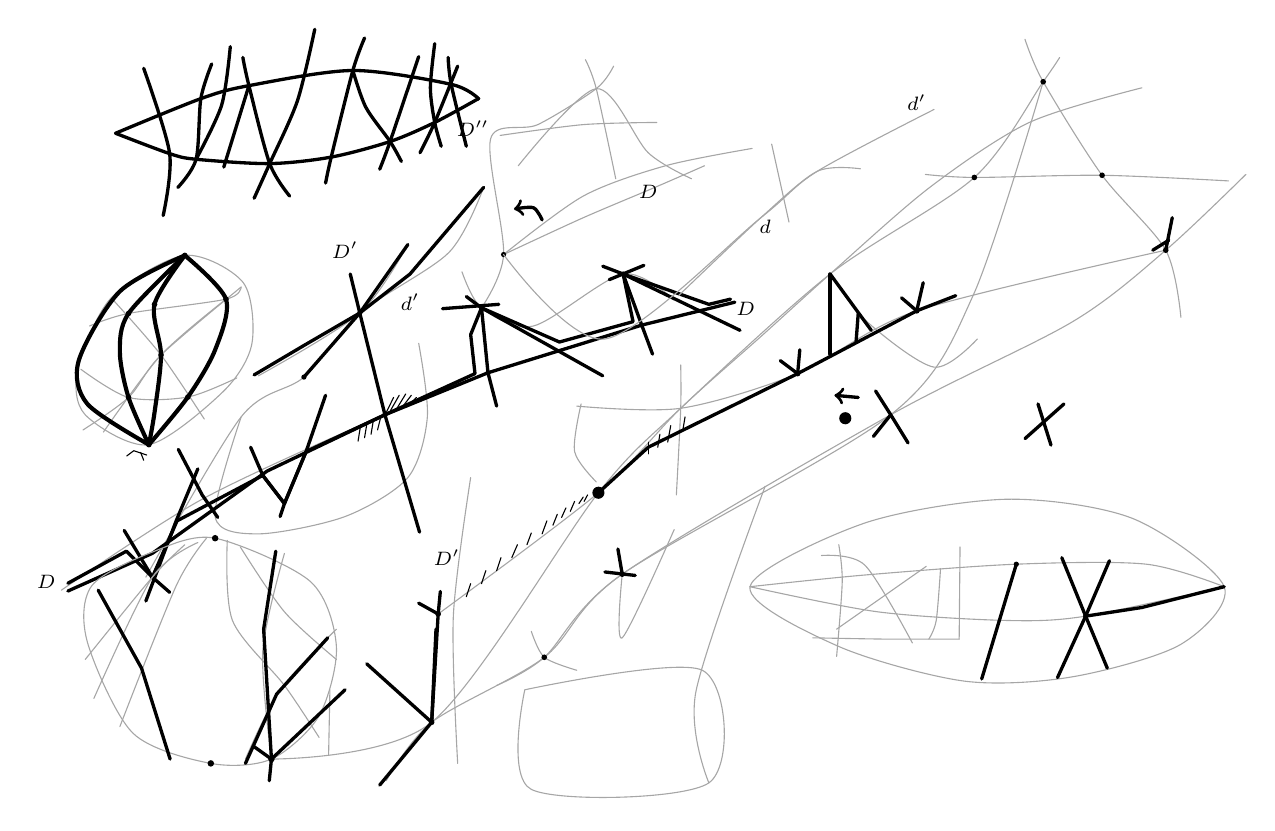
\begin{tikzpicture}[x=.55cm,y=-.55cm,line cap=round,line join=round,g/.style={olive!80!yellow,line width=1.7pt},r/.style={orange!80!brown,line width=1.8pt},w/.style={red!60!black,line width=1.5pt},b/.style={blue!60!black,line width=1.4pt},p/.style={gray!70,thin},k/.style={black,line width=1.2pt},every node/.style={font=\scriptsize}]
% Upper-left lens and crossing strands.
\draw[k] plot[smooth] coordinates {(2.7,4.75) (4.67,3.95) (5.78,3.65) (8.18,3.3) (10.45,3.62) (11.08,3.95)};
\draw[k] plot[smooth] coordinates {(2.7,4.75) (3.95,5.22) (4.56,5.35) (6.26,5.45) (7.68,5.3) (9.04,4.94) (10.07,4.5) (11.08,3.95)};
\draw[k] plot[smooth] coordinates {(3.35,3.25) (3.95,5.22) (3.8,6.65)};
\draw[k] plot[smooth] coordinates {(4.92,3.15) (4.67,3.95) (4.56,5.35) (4.14,6.0)};
\draw[k] plot[smooth] coordinates {(5.35,2.75) (5.15,4.1) (4.56,5.35)};
\draw[k] plot[smooth] coordinates {(5.78,3.65) (5.2,5.53)};
\draw[k] plot[smooth] coordinates {(5.64,3.0) (5.78,3.65) (6.26,5.45) (6.72,6.2)};
\draw[k] plot[smooth] coordinates {(7.3,2.35) (6.9,4.0) (6.26,5.45) (5.9,6.25)};
\draw[k] plot[smooth] coordinates {(8.45,2.55) (8.18,3.3) (7.68,5.3) (7.55,5.9)};
\draw[k] plot[smooth] coordinates {(8.18,3.3) (8.48,4.15) (9.04,4.94) (9.3,5.4)};
\draw[k] plot[smooth] coordinates {(9.7,2.98) (9.04,4.94) (8.8,5.58)};
\draw[k] plot[smooth] coordinates {(10.07,2.68) (9.97,3.7) (10.07,4.5) (10.22,5.05)};
\draw[k] plot[smooth] coordinates {(10.38,3.0) (10.45,3.62) (10.8,5.05)};
\draw[k] plot[smooth] coordinates {(10.6,3.2) (10.07,4.5) (9.73,5.2)};
\fill[k] (3.95,5.22) circle (.045);
\fill[k] (4.67,3.95) circle (.045);
\fill[k] (4.56,5.35) circle (.045);
\fill[k] (5.78,3.65) circle (.045);
\fill[k] (6.26,5.45) circle (.045);
\fill[k] (8.18,3.3) circle (.045);
\fill[k] (7.68,5.3) circle (.045);
\fill[k] (9.04,4.94) circle (.045);
\fill[k] (10.07,4.5) circle (.045);
\fill[k] (10.45,3.62) circle (.045);
\fill[k] (11.08,3.95) circle (.045);
\node at (10.95,4.65) {$D^{\prime\prime}$};
% Left middle globe, with pencil arcs behind ink arcs.
\draw[p] plot[smooth cycle] coordinates {(4.3,7.57) (5.65,8.2) (5.85,9.6) (5.2,10.7) (3.47,11.94) (2.0,11.25) (1.83,10.2) (2.6,8.55)};
\draw[p] plot[smooth] coordinates {(1.9,10.2) (3.0,10.85) (4.37,10.84) (5.5,10.4)};
\draw[p] plot[smooth] coordinates {(2.1,9.2) (3.0,8.91) (5.25,8.58) (5.6,8.3)};
\draw[p] plot[smooth] coordinates {(2.42,11.65) (3.75,9.87) (5.25,8.58)};
\draw[p] plot[smooth] coordinates {(2.6,8.55) (3.75,9.87) (4.75,11.35)};
\draw[p] plot[smooth] coordinates {(1.95,11.6) (3.0,10.85) (3.75,9.87) (5.6,8.3)};
\draw[k,line width=1.5pt] plot[smooth] coordinates {(4.3,7.57) (2.8,8.4) (1.85,10.0) (2.05,11.0) (3.47,11.94)};
\draw[k,line width=1.5pt] plot[smooth] coordinates {(4.3,7.57) (5.25,8.58) (5.0,9.75) (4.37,10.84) (3.47,11.94)};
\draw[k,line width=1.5pt] plot[smooth] coordinates {(4.3,7.57) (3.0,8.91) (2.8,9.8) (3.0,10.85) (3.47,11.94)};
\draw[k,line width=1.5pt] plot[smooth] coordinates {(4.3,7.57) (3.6,8.7) (3.75,9.87) (3.6,11.2) (3.47,11.94)};
\fill[k] (4.3,7.57) circle (.065);
\fill[k] (3.0,8.91) circle (.065);
\fill[k] (3.6,8.7) circle (.065);
\fill[k] (5.25,8.58) circle (.065);
\fill[k] (3.75,9.87) circle (.065);
\fill[k] (3.0,10.85) circle (.065);
\fill[k] (4.37,10.84) circle (.065);
\fill[k] (3.47,11.94) circle (.065);
\draw[k,thin] (2.96,12.2)--(3.12,12.08)--(3.42,12.18);
\draw[k,thin] (3.28,12.12)--(3.35,12.3);
% Central oblique line D and its black/pencil crossing sketches.
\draw[p] plot[smooth] coordinates {(1.45,15.3) (4.7,13.2) (8.9,11.25) (11.3,10.28) (14.85,9.18) (17.0,8.65)};
\draw[p] plot[smooth] coordinates {(3.4,15.0) (5.6,11.3) (7.05,10.38) (8.34,8.9) (10.4,7.5) (11.2,6.0)};
\draw[p] plot[smooth] coordinates {(6.0,10.35) (8.34,8.9) (9.45,7.32)};
\draw[p] plot[smooth] coordinates {(8.34,8.9) (8.92,11.25) (9.72,13.96)};
\draw[p] plot[smooth] coordinates {(5.6,11.3) (5.0,13.6) (6.0,14.0) (8.0,13.6) (9.45,12.7) (9.9,11.3) (9.7,9.6)};
\draw[p] plot[smooth] coordinates {(10.7,7.95) (11.15,8.78) (12.35,9.2) (14.42,8.0) (15.6,8.6)};
\draw[p] plot[smooth] coordinates {(11.15,8.78) (11.66,7.55) (11.36,4.88) (12.45,4.55) (13.8,3.72) (14.2,3.2)};
\draw[p] plot[smooth] coordinates {(11.66,7.55) (13.5,6.7) (15.2,5.98) (16.3,5.5)};
\draw[p] plot[smooth] coordinates {(12.0,5.5) (13.8,3.72) (15.0,5.2) (16.0,5.8)};
\draw[p] plot[smooth] coordinates {(13.55,3.05) (13.8,3.72) (14.25,5.8)};
\draw[p] plot[smooth] coordinates {(11.58,4.8) (13.5,4.55) (15.2,4.5)};
\draw[p] plot[smooth] coordinates {(11.66,7.55) (13.5,6.2) (15.4,5.5) (17.4,5.1)};
\draw[k] (1.6,15.14)--(2.95,14.4)--(3.55,15.0)--(4.12,13.7)--(6.1,12.65)--(6.6,13.3)--(7.1,12.1)--(8.92,11.25)--(11.0,10.3)--(10.9,9.4)--(11.15,8.78)--(12.95,9.57)--(14.65,9.1)--(14.42,8.0)--(16.4,8.7)--(16.9,8.58);
\draw[k] (1.6,15.32)--(3.55,14.45)--(6.2,12.55)--(8.92,11.25)--(11.3,10.28)--(14.85,9.18)--(17.0,8.65);
\draw[k] (3.4,15.55)--(4.1,13.7)--(4.6,12.5);
\draw[k] (2.9,13.92)--(3.55,15.0)--(3.95,15.35);
\draw[k] (4.15,12.05)--(4.7,13.1)--(5.06,13.62);
\draw[k] (5.82,12.0)--(6.1,12.65)--(6.6,13.3)--(6.5,13.6);
\draw[k] (7.55,10.8)--(7.1,12.1)--(6.6,13.3);
\draw[k] (5.9,10.33)--(7.05,9.65)--(8.34,8.9)--(9.45,7.32);
\draw[k] (7.05,10.38)--(8.34,8.9)--(9.5,8.0)--(11.2,6.0);
\draw[k] (8.12,8.0)--(8.34,8.9)--(8.92,11.25)--(9.72,13.96);
\draw[k] (10.8,8.52)--(11.15,8.78)--(13.95,10.35);
\draw[k] (11.15,8.78)--(11.3,10.28)--(11.5,11.05);
\draw[k] (10.25,8.8)--(11.55,8.7);
\draw[k] (13.95,7.82)--(14.42,8.0)--(17.12,9.3);
\draw[k] (14.42,8.0)--(14.85,9.18)--(15.1,9.85);
\draw[k] (14.1,8.13)--(14.9,7.8);
\draw[k,thin] (8.3,11.86)--(8.35,11.55);
\draw[k,thin] (8.45,11.78)--(8.5,11.48);
\draw[k,thin] (8.6,11.7)--(8.65,11.4);
\draw[k,thin] (8.75,11.6)--(8.82,11.32);
\draw[k,thin] (8.95,11.2)--(9.12,10.85);
\draw[k,thin] (9.05,11.15)--(9.25,10.8);
\draw[k,thin] (9.18,11.13)--(9.4,10.77);
\draw[k,thin] (9.3,11.1)--(9.53,10.8);
\draw[k,thin] (9.42,11.07)--(9.65,10.85);
\fill[k] (3.55,15.0) circle (.06);
\fill[k] (7.05,10.38) circle (.06);
\fill[k] (8.34,8.9) circle (.06);
\fill[k] (8.92,11.25) circle (.06);
\fill[k] (11.15,8.78) circle (.06);
\fill[k] (11.3,10.28) circle (.06);
\fill[k] (14.42,8.0) circle (.06);
\fill[k] (14.85,9.18) circle (.06);
\fill[k] (11.66,7.55) circle (.06);
\node at (1.1,15.12) {$D$};
\node at (8.0,7.45) {$D^{\prime}$};
\node at (9.5,8.65) {$\unsure{d^{\prime}}$};
\node at (15.0,6.1) {$D$};
\node at (17.25,8.8) {$D$};
\node at (10.35,14.55) {$\unsure{D^{\prime}}$};
\draw[k,->] plot[smooth] coordinates {(12.55,6.75) (12.35,6.47) (11.9,6.5)};
% Upper-right and central-right pencil arrangement and darker local pieces.
\draw[p] plot[smooth] coordinates {(10.15,15.85) (13.85,13.05) (15.75,11.1) (17.65,9.4) (19.2,8.0) (21.5,6.0) (23.8,4.5) (26.4,3.7)};
\draw[p] plot[smooth] coordinates {(6.3,19.2) (10.0,18.35) (13.85,13.05) (15.75,11.1) (19.2,8.0) (22.53,5.77) (24.12,3.56) (24.5,3.0)};
\draw[p] plot[smooth] coordinates {(8.95,19.7) (10.0,18.35) (12.6,16.85) (14.4,14.93) (20.6,11.25) (24.8,9.1) (26.95,7.45) (28.8,5.7)};
\draw[p] plot[smooth] coordinates {(11.5,17.5) (12.6,16.85) (14.4,14.93) (20.6,11.25) (22.5,8.5) (24.12,3.56)};
\draw[p] plot[smooth] coordinates {(11.66,7.55) (14.0,9.5) (17.6,6.7) (18.9,5.63) (21.6,4.2)};
\draw[p] plot[smooth] coordinates {(15.7,8.5) (17.6,6.7) (18.9,5.63) (19.9,5.57)};
\draw[p] plot[smooth] coordinates {(17.85,5.0) (18.25,6.8)};
\draw[p] plot[smooth] coordinates {(13.35,11.05) (15.75,11.1) (18.45,10.3) (21.2,8.85) (26.95,7.45)};
\draw[p] plot[smooth] coordinates {(21.4,5.7) (22.53,5.77) (25.48,5.72) (28.4,5.85)};
\draw[p] plot[smooth] coordinates {(23.7,2.58) (24.12,3.56) (25.48,5.72) (26.95,7.45) (27.3,9.0)};
\draw[p] plot[smooth] coordinates {(19.2,8.0) (20.05,9.1) (21.6,10.15) (22.6,9.5)};
\draw[p] plot[smooth] coordinates {(13.8,12.8) (13.3,12.1) (13.45,11.0)};
\draw[p] plot[smooth] coordinates {(15.75,10.1) (15.75,11.1) (15.65,13.1)};
\draw[p] plot[smooth] coordinates {(14.4,14.93) (14.4,16.4) (15.6,13.9)};
\draw[p] plot[smooth] coordinates {(12.3,16.25) (12.6,16.85) (13.35,17.15)};
\draw[p] plot[smooth] coordinates {(17.7,12.9) (16.1,17.65) (16.4,19.75)};
\draw[p] plot[smooth] coordinates {(10.9,12.7) (10.5,15.9) (10.6,19.3)};
\draw[p] plot[smooth] coordinates {(12.15,17.6) (16.25,17.15) (16.4,19.75) (12.3,19.9) (12.15,17.6)};
\draw[k] (13.85,13.05)--(15.0,12.0)--(18.45,10.3)--(21.2,8.85);
\draw[k] (10.15,15.85)--(10.0,18.35)--(8.8,19.8);
\draw[k] (18.45,10.3)--(18.05,10.0);
\draw[k] (18.45,10.3)--(18.5,9.75);
\draw[k] (21.2,8.85)--(20.85,8.55);
\draw[k] (21.2,8.85)--(21.35,8.2);
\draw[k] (21.2,8.85)--(22.1,8.5);
\draw[k] (19.2,8.0)--(19.2,9.85);
\draw[k] (19.2,8.0)--(20.15,9.3);
\draw[k] (19.85,8.9)--(19.8,9.56);
\draw[k] (26.95,7.45)--(27.1,6.7);
\draw[k] (26.65,7.45)--(27.02,7.22);
\draw[k] (24.0,11.0)--(24.3,11.95);
\draw[k] (23.7,11.8)--(24.6,11.0);
\draw[k] (14.4,14.93)--(14.3,14.35);
\draw[k] (14.0,14.88)--(14.7,14.96);
\draw[k] (10.15,15.85)--(9.7,15.6);
\draw[k] (10.15,15.85)--(10.2,15.33);
\draw[k] (8.5,17.0)--(10.0,18.35)--(10.1,16.2);
\draw[k] (20.6,11.25)--(20.25,10.7);
\draw[k] (20.6,11.25)--(21.0,11.9);
\draw[k] (20.6,11.25)--(20.2,11.75);
\fill[k] (24.12,3.56) circle (.065);
\fill[k] (22.53,5.77) circle (.065);
\fill[k] (25.48,5.72) circle (.065);
\fill[k] (26.95,7.45) circle (.065);
\fill[k] (18.45,10.3) circle (.065);
\fill[k] (21.2,8.85) circle (.065);
\fill[k] (10.15,15.85) circle (.065);
\fill[k] (10.0,18.35) circle (.065);
\fill[k] (12.6,16.85) circle (.065);
\fill[k] (14.4,14.93) circle (.065);
\fill[k] (13.85,13.05) circle (.14);
\fill[k] (19.55,11.33) circle (.14);
\draw[k,thin] (10.8,15.45)--(10.9,15.15);
\draw[k,thin] (11.15,15.15)--(11.25,14.85);
\draw[k,thin] (11.5,14.85)--(11.6,14.55);
\draw[k,thin] (11.85,14.55)--(11.98,14.25);
\draw[k,thin] (12.2,14.25)--(12.3,13.98);
\draw[k,thin] (12.55,14.0)--(12.66,13.7);
\draw[k,thin] (12.8,13.8)--(12.9,13.55);
\draw[k,thin] (13.0,13.62)--(13.1,13.4);
\draw[k,thin] (13.2,13.48)--(13.3,13.25);
\draw[k,thin] (13.4,13.3)--(13.5,13.15);
\draw[k,thin] (13.52,13.25)--(13.6,13.1);
\draw[k,thin] (15.0,12.15)--(15.0,11.88);
\draw[k,thin] (15.22,12.0)--(15.27,11.7);
\draw[k,thin] (15.45,11.88)--(15.52,11.5);
\draw[k,thin] (15.8,11.6)--(15.85,11.3);
\node at (21.2,4.05) {$d^{\prime}$};
\node at (17.7,6.9) {$d$};
\draw[k,->] plot[smooth] coordinates {(19.85,10.85) (19.3,10.8)};
% Lower-left circle with crossing arcs.
\draw[p] plot[smooth cycle] coordinates {(5.0,14.1) (7.2,15.1) (7.8,16.6) (7.4,18.2) (6.3,19.2) (4.9,19.3) (3.1,18.6) (2.05,16.5) (2.15,15.2) (3.6,14.4)};
\draw[p] plot[smooth] coordinates {(2.2,17.8) (3.55,15.0) (4.6,14.2)};
\draw[p] plot[smooth] coordinates {(2.8,18.45) (4.1,15.2) (4.8,14.1)};
\draw[p] plot[smooth] coordinates {(2.0,16.9) (3.55,15.0) (4.3,14.25)};
\draw[p] plot[smooth] coordinates {(5.28,14.15) (5.4,16.0) (6.6,17.5) (7.4,18.7)};
\draw[p] plot[smooth] coordinates {(5.58,14.3) (6.6,15.8) (7.8,16.9)};
\draw[p] plot[smooth] coordinates {(7.8,16.2) (6.5,17.6) (5.7,19.2)};
\draw[p] plot[smooth] coordinates {(7.65,17.6) (7.62,19.1)};
\draw[p] plot[smooth] coordinates {(6.6,14.45) (6.1,16.7) (6.3,19.2)};
\draw[k] (2.3,15.3)--(3.3,17.1)--(3.96,19.2);
\draw[k] (6.4,14.4)--(6.12,16.2)--(6.3,19.2);
\draw[k] (7.6,16.4)--(6.42,17.7)--(5.7,19.3);
\draw[k] (6.3,19.2)--(8.0,17.6);
\draw[k] (5.88,18.9)--(6.3,19.2)--(6.25,19.7);
\fill[k] (5.0,14.1) circle (.075);
\fill[k] (4.9,19.3) circle (.075);
\fill[k] (6.3,19.2) circle (.075);
% Lower-right elongated lens, with two dark marked crossings.
\draw[p] plot[smooth cycle] coordinates {(17.35,15.22) (20.0,13.75) (23.3,13.2) (26.2,13.65) (28.3,15.22) (27.3,16.55) (24.8,17.3) (22.3,17.4) (19.4,16.6)};
\draw[p] plot[smooth] coordinates {(17.35,15.22) (20.0,14.95) (23.5,14.7) (26.5,14.7) (28.3,15.22)};
\draw[p] plot[smooth] coordinates {(17.35,15.22) (20.3,15.8) (23.3,16.0) (25.1,15.9) (28.3,15.22)};
\draw[p] plot[smooth] coordinates {(19.4,14.25) (19.48,15.1) (19.35,16.83)};
\draw[p] plot[smooth] coordinates {(19.0,14.5) (20.0,14.72) (21.1,16.52)};
\draw[p] plot[smooth] coordinates {(19.35,16.2) (21.42,14.75)};
\draw[p] plot[smooth] coordinates {(22.2,14.3) (22.18,16.43)};
\draw[p] plot[smooth] coordinates {(21.75,14.8) (21.65,16.0) (21.48,16.43)};
\draw[p] plot[smooth] coordinates {(18.8,16.4) (20.5,16.43) (22.18,16.43)};
\draw[k] (22.7,17.35)--(23.5,14.7);
\draw[k] (24.55,14.55)--(25.1,15.9)--(25.6,17.1);
\draw[k] (25.65,14.62)--(25.1,15.9)--(24.45,17.32);
\draw[k] (25.1,15.9)--(26.4,15.7)--(28.3,15.22);
\fill[k] (23.5,14.7) circle (.06);
\fill[k] (25.1,15.9) circle (.06);
\end{tikzpicture}}

$p.r.$ \unsure{stble|stable}\\
$p.r.$ \unsure{semi-stbles|semi-stables}\\
$p.r.$ \uline{critiques} (\unsure{on réserve pour}\\
\unsure{la spécialisation})

\[n\frac{(n-1)(n-2)}{2}\]
\[
\frac12\frac{n(n-1)}2\left(\frac{n(n-1)}2-1\right)
-\frac{n(n-1)(\unsure{n-1|n-2})}{2}
=\quad\deleted{\unsure{n+2}}\quad\sim\frac18n^4
\]
\margin{\mspage{141}}

\scanpage{143}
{\color{gray}\ttfamily
\unsure{****A}\quad\unsure{CRAY2}\quad\unsure{0025}\quad\unsure{1}
}
{\color{gray}\scriptsize\unsure{
\begin{tabular}{l}
\texttt{\ \ \ \ \ \ \ \ \ \ \ 00000000\ \ \ \ \ \ 00000000\ \ \ \ \ \ 00000000\ \ \ \ \ \ 00000000}\\
\texttt{\ \ \ \ \ \ \ \ \ 0000000000\ \ \ \ 0000000000\ \ \ \ 0000000000\ \ \ \ 0000000000}\\
\texttt{\ \ \ \ \ \ \ 00\ \ \ \ \ \ 0000\ \ 00\ \ \ \ \ \ 0000\ \ 00\ \ \ \ \ \ 0000\ \ 00\ \ \ \ \ \ 0000}\\
\texttt{\ \ \ \ \ \ 00\ \ \ \ \ 00\ 00\ \ 00\ \ \ \ \ 00\ 00\ \ 00\ \ \ \ \ 00\ 00\ \ 00\ \ \ \ \ 00\ 00}\\
\texttt{\ \ \ \ \ 00\ \ \ \ 00\ \ 00\ \ 00\ \ \ \ 00\ \ 00\ \ 00\ \ \ \ 00\ \ 00\ \ 00\ \ \ \ 00\ \ 00}\\
\texttt{\ \ \ \ 00\ \ \ 00\ \ \ 00\ \ 00\ \ \ 00\ \ \ 00\ \ 00\ \ \ 00\ \ \ 00\ \ 00\ \ \ 00\ \ \ 00}\\
\texttt{\ \ \ 00\ \ 00\ \ \ \ 00\ \ 00\ \ 00\ \ \ \ 00\ \ 00\ \ 00\ \ \ \ 00\ \ 00\ \ 00\ \ \ \ 00}\\
\texttt{\ \ 00\ 00\ \ \ \ \ 00\ \ 00\ 00\ \ \ \ \ 00\ \ 00\ 00\ \ \ \ \ 00\ \ 00\ 00\ \ \ \ \ 00}\\
\texttt{\ 0000\ \ \ \ \ \ 00\ \ 0000\ \ \ \ \ \ 00\ \ 0000\ \ \ \ \ \ 00\ \ 0000\ \ \ \ \ \ 00}\\
\texttt{000\ \ \ \ \ \ \ 00\ \ 000\ \ \ \ \ \ \ 00\ \ 000\ \ \ \ \ \ \ 00\ \ 000\ \ \ \ \ \ \ 00}\\
\texttt{0000000000\ \ \ \ 0000000000\ \ \ \ 0000000000\ \ \ \ 0000000000}\\
\texttt{00000000\ \ \ \ \ \ 00000000\ \ \ \ \ \ 00000000\ \ \ \ \ \ 00000000}\\
\texttt{}\\
\texttt{\ CCCCCCCCCC\ \ \ RRRRRRRRRRR\ \ \ \ AAAAAAAAAA\ \ \ YY\ \ \ \ \ \ \ \ YY\ \ \ 2222222222}\\
\texttt{CCCCCCCCCCCC\ \ RRRRRRRRRRRR\ \ AAAAAAAAAAAA\ \ YY\ \ \ \ \ \ \ \ YY\ \ 222222222222}\\
\texttt{CC\ \ \ \ \ \ \ \ CC\ \ RR\ \ \ \ \ \ \ \ RR\ \ AA\ \ \ \ \ \ \ \ AA\ \ \ YY\ \ \ \ \ \ YY\ \ 22\ \ \ \ \ \ \ \ 22}\\
\texttt{CC\ \ \ \ \ \ \ \ \ \ \ \ RR\ \ \ \ \ \ \ \ RR\ \ AA\ \ \ \ \ \ \ \ AA\ \ \ \ YY\ \ \ \ YY\ \ \ \ \ \ \ \ \ \ \ \ 22}\\
\texttt{CC\ \ \ \ \ \ \ \ \ \ \ \ RR\ \ \ \ \ \ \ \ RR\ \ AA\ \ \ \ \ \ \ \ AA\ \ \ \ \ YY\ \ YY\ \ \ \ \ \ \ \ \ \ \ \ \ 22}\\
\texttt{CC\ \ \ \ \ \ \ \ \ \ \ \ RRRRRRRRRRRR\ \ AAAAAAAAAAAA\ \ \ \ \ \ YYYY\ \ \ \ \ \ \ \ \ \ \ \ \ \ 22}\\
\texttt{CC\ \ \ \ \ \ \ \ \ \ \ \ RRRRRRRRRRR\ \ \ AAAAAAAAAAAA\ \ \ \ \ \ \ YY\ \ \ \ \ \ \ \ \ \ \ \ \ 22}\\
\texttt{CC\ \ \ \ \ \ \ \ \ \ \ \ RR\ \ \ \ RR\ \ \ \ \ \ AA\ \ \ \ \ \ \ \ AA\ \ \ \ \ \ \ YY\ \ \ \ \ \ \ \ \ \ \ 22}\\
\texttt{CC\ \ \ \ \ \ \ \ \ \ \ \ RR\ \ \ \ \ RR\ \ \ \ \ AA\ \ \ \ \ \ \ \ AA\ \ \ \ \ \ \ YY\ \ \ \ \ \ \ \ \ 22}\\
\texttt{CC\ \ \ \ \ \ \ \ CC\ \ RR\ \ \ \ \ \ RR\ \ \ \ AA\ \ \ \ \ \ \ \ AA\ \ \ \ \ \ \ YY\ \ \ \ \ \ \ 22}\\
\texttt{CCCCCCCCCCCC\ \ RR\ \ \ \ \ \ \ RR\ \ \ AA\ \ \ \ \ \ \ \ AA\ \ \ \ \ \ \ YY\ \ \ \ \ \ 222222222222}\\
\texttt{\ CCCCCCCCCC\ \ \ RR\ \ \ \ \ \ \ \ RR\ \ AA\ \ \ \ \ \ \ \ AA\ \ \ \ \ \ \ YY\ \ \ \ \ \ 222222222222}\\
\end{tabular}}}
{\color{gray}\ttfamily ****A\quad END\quad JOB\quad25\quad CRAY2\quad ROOM\quad 9.03.23 AM 19 AUG 82\quad\unsure{R6.PR1}\quad SYS JES2\quad JOB\quad25\quad END\quad A****}\\
{\color{gray}\ttfamily ****A\quad END\quad JOB\quad25\quad CRAY2\quad ROOM\quad 9.03.23 AM 19 AUG 82\quad\unsure{R6.PR1}\quad SYS JES2\quad JOB\quad25\quad END\quad A****}\\
{\color{gray}\ttfamily ****A\quad END\quad JOB\quad25\quad CRAY2\quad ROOM\quad 9.03.23 AM 19 AUG 82\quad\unsure{R6.PR1}\quad SYS JES2\quad JOB\quad25\quad END\quad A****}\\
{\color{gray}\ttfamily ****A\quad END\quad JOB\quad25\quad CRAY2\quad ROOM\quad 9.03.23 AM 19 AUG 82\quad\unsure{R6.PR1}\quad SYS JES2\quad JOB\quad25\quad END\quad A****}\\
{\color{gray}\ttfamily ****A\quad END\quad JOB\quad25\quad CRAY2\quad ROOM\quad 9.03.23 AM 19 AUG 82\quad\unsure{R6.PR1}\quad SYS JES2\quad JOB\quad25\quad END\quad A****}\\
{\color{gray}\ttfamily ****A\quad END\quad JOB\quad25\quad CRAY2\quad ROOM\quad 9.03.23 AM 19 AUG 82\quad\unsure{R6.PR1}\quad SYS JES2\quad JOB\quad25\quad END\quad A****}\\
\figure{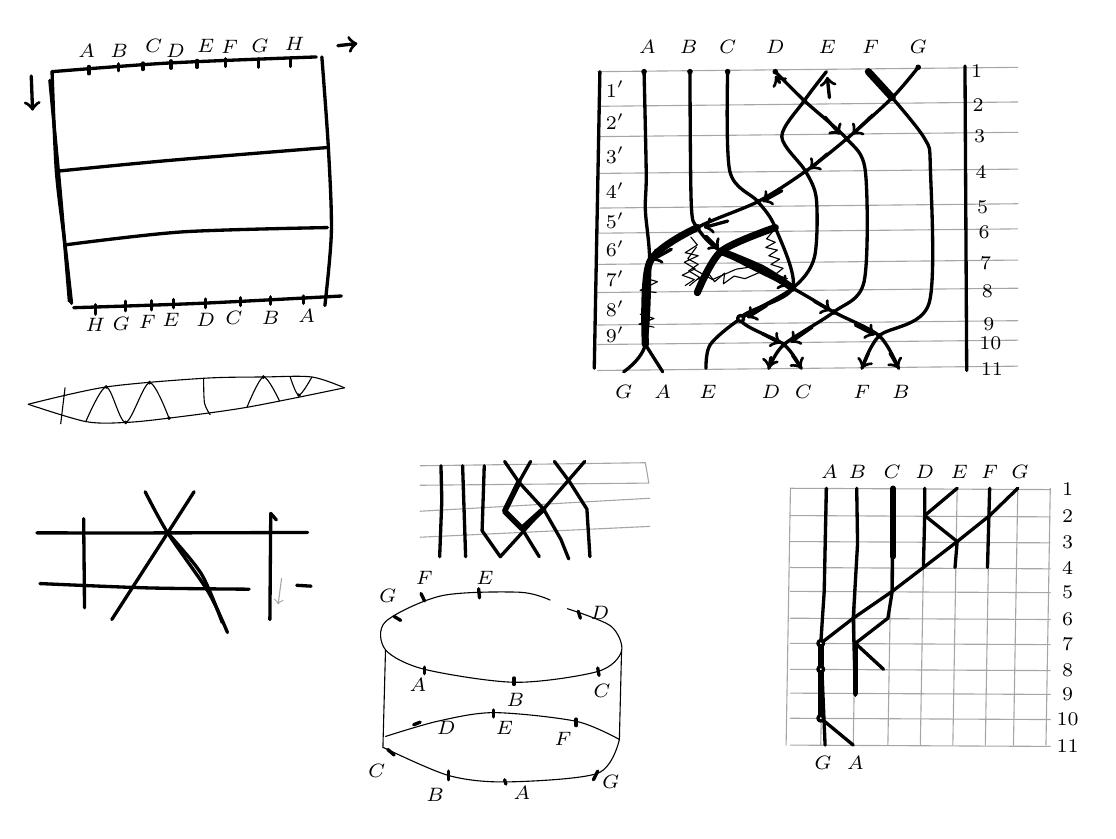
\begin{tikzpicture}[x=.55cm,y=-.55cm,line cap=round,line join=round,g/.style={olive!80!yellow,line width=1.7pt},r/.style={orange!80!brown,line width=1.8pt},w/.style={red!60!black,line width=1.5pt},b/.style={blue!60!black,line width=1.4pt},p/.style={gray!70,thin},k/.style={black,line width=1.2pt},every node/.style={font=\scriptsize}]
% Upper-left frame with opposed written orders.
\draw[k] plot[smooth] coordinates {(1.8,2.3) (4.5,2.1) (7.9,1.96)};
\draw[k] plot[smooth] coordinates {(1.8,2.3) (1.9,4.6) (2.1,6.3) (2.25,7.65)};
\draw[k] plot[smooth] coordinates {(1.75,2.5) (2.0,5.2) (2.2,7.6)};
\draw[k] plot[smooth] coordinates {(8.03,1.96) (8.18,4.05) (8.25,6.0) (8.1,7.7)};
\draw[k] plot[smooth] coordinates {(1.9,4.6) (4.5,4.35) (8.18,4.05)};
\draw[k] plot[smooth] coordinates {(2.1,6.3) (4.8,6.0) (8.16,5.9)};
\draw[k] plot[smooth] coordinates {(2.3,7.75) (5.2,7.65) (8.48,7.48)};
\draw[k,->] (1.32,2.4)--(1.35,3.2);
\draw[k,->] (8.4,1.7)--(8.85,1.65);
\node at (2.6,1.83) {$A$};
\node at (3.35,1.83) {$B$};
\node at (4.15,1.7) {$C$};
\node at (4.65,1.83) {$D$};
\node at (5.35,1.7) {$E$};
\node at (5.9,1.73) {$F$};
\node at (6.6,1.7) {$G$};
\node at (7.4,1.65) {$H$};
\node at (2.8,8.15) {$H$};
\node at (3.4,8.12) {$G$};
\node at (4.0,8.08) {$F$};
\node at (4.55,8.03) {$E$};
\node at (5.35,8.03) {$D$};
\node at (6.0,7.98) {$C$};
\node at (6.85,7.98) {$B$};
\node at (7.68,7.95) {$A$};
\draw[k] (2.65,2.18)--(2.65,2.35);
\draw[k] (3.34,2.12)--(3.34,2.28);
\draw[k] (3.9,2.1)--(3.9,2.25);
\draw[k] (4.55,2.05)--(4.55,2.22);
\draw[k] (5.15,2.04)--(5.15,2.2);
\draw[k] (5.8,2.0)--(5.8,2.18);
\draw[k] (6.56,2.0)--(6.56,2.2);
\draw[k] (7.3,1.98)--(7.3,2.18);
\draw[k] (2.8,7.68)--(2.8,7.9);
\draw[k] (3.5,7.6)--(3.5,7.82);
\draw[k] (4.1,7.59)--(4.1,7.8);
\draw[k] (4.6,7.56)--(4.6,7.75);
\draw[k] (5.35,7.55)--(5.35,7.75);
\draw[k] (6.15,7.52)--(6.15,7.7);
\draw[k] (6.85,7.5)--(6.85,7.67);
\draw[k] (7.6,7.48)--(7.6,7.65);
% Large upper-right numbered grid with strands and arrows.
\draw[p] (14.4,2.3)--(24.1,2.1999999999999997);
\node at (23.15,2.28) {$1$};
\node at (14.8,2.7) {$1'$};
\draw[p] (14.4,3.1)--(24.1,3.0);
\node at (23.185,3.08) {$2$};
\node at (14.8,3.45) {$2'$};
\draw[p] (14.4,3.8)--(24.1,3.6999999999999997);
\node at (23.22,3.78) {$3$};
\node at (14.8,4.225) {$3'$};
\draw[p] (14.4,4.65)--(24.1,4.550000000000001);
\node at (23.255,4.630000000000001) {$4$};
\node at (14.8,5.050000000000001) {$4'$};
\draw[p] (14.4,5.45)--(24.1,5.3500000000000005);
\node at (23.29,5.430000000000001) {$5$};
\node at (14.8,5.74) {$5'$};
\draw[p] (14.4,6.03)--(24.1,5.930000000000001);
\node at (23.325,6.010000000000001) {$6$};
\node at (14.8,6.390000000000001) {$6'$};
\draw[p] (14.4,6.75)--(24.1,6.65);
\node at (23.36,6.73) {$7$};
\node at (14.8,7.075) {$7'$};
\draw[p] (14.4,7.4)--(24.1,7.300000000000001);
\node at (23.395,7.380000000000001) {$8$};
\node at (14.8,7.775) {$8'$};
\draw[p] (14.4,8.15)--(24.1,8.05);
\node at (23.43,8.13) {$9$};
\node at (14.8,8.375) {$9'$};
\draw[p] (14.4,8.6)--(24.1,8.5);
\node at (23.465,8.58) {$10$};
\draw[p] (14.4,9.2)--(24.1,9.1);
\node at (23.5,9.18) {$11$};
\draw[k] plot[smooth] coordinates {(14.45,2.3) (14.32,9.15)};
\draw[k] plot[smooth] coordinates {(22.88,2.17) (22.92,9.2)};
\draw[k] plot[smooth] coordinates {(15.47,2.3) (15.52,4.65) (15.5,5.5) (15.6,6.7) (15.5,8.6) (15.0,9.23)};
\draw[k] plot[smooth] coordinates {(15.5,8.6) (15.9,9.23)};
\draw[k] plot[smooth] coordinates {(16.53,2.3) (16.56,5.35) (16.7,5.9) (17.25,6.45) (18.9,7.3) (19.85,7.85) (20.9,8.4) (21.35,9.15)};
\draw[k] plot[smooth] coordinates {(17.4,2.3) (17.45,4.6) (18.1,5.3) (18.5,5.9) (18.9,7.3) (17.7,8.0) (18.7,8.6) (19.1,9.15)};
\draw[k] plot[smooth] coordinates {(18.5,2.3) (19.17,2.97) (20.15,3.85) (20.58,4.6) (20.55,7.15) (19.85,7.85) (18.7,8.6) (18.35,9.15)};
\draw[k] plot[smooth] coordinates {(19.68,2.3) (19.17,2.97) (18.65,3.8) (19.2,4.6) (19.45,5.25) (19.4,6.6) (18.9,7.3) (17.7,8.0) (17.0,8.6) (16.9,9.15)};
\draw[k] plot[smooth] coordinates {(20.65,2.3) (21.2,2.9) (21.95,3.85) (22.08,4.5) (22.05,7.65) (20.9,8.4) (20.5,9.15)};
\draw[k] plot[smooth] coordinates {(21.8,2.2) (21.2,2.9) (20.15,3.85) (19.2,4.6) (18.1,5.3) (16.7,5.9) (15.6,6.7) (15.5,8.6)};
\draw[k,line width=2.6pt] plot[smooth] coordinates {(20.65,2.3) (21.2,2.9)};
\draw[k,line width=2.6pt] plot[smooth] coordinates {(16.7,5.9) (15.6,6.7) (15.5,8.6)};
\draw[k,line width=2.6pt] plot[smooth] coordinates {(16.7,7.4) (17.25,6.45) (18.5,5.9)};
\draw[k,line width=2.6pt] plot[smooth] coordinates {(17.25,6.45) (18.2,6.85) (18.9,7.3)};
\fill[k] (15.47,2.3) circle (.065);
\fill[k] (16.53,2.3) circle (.065);
\fill[k] (17.4,2.3) circle (.065);
\fill[k] (18.5,2.3) circle (.065);
\fill[k] (19.17,2.97) circle (.065);
\fill[k] (21.2,2.9) circle (.065);
\fill[k] (21.8,2.2) circle (.065);
\fill[k] (20.15,3.85) circle (.065);
\fill[k] (19.2,4.6) circle (.065);
\fill[k] (18.1,5.3) circle (.065);
\fill[k] (16.7,5.9) circle (.065);
\fill[k] (17.25,6.45) circle (.065);
\fill[k] (15.6,6.7) circle (.065);
\fill[k] (18.9,7.3) circle (.065);
\fill[k] (19.85,7.85) circle (.065);
\fill[k] (20.9,8.4) circle (.065);
\fill[k] (18.7,8.6) circle (.065);
\draw[k,fill=white] (17.7,8.0) circle (.07);
\draw[k,->] (18.6,2.55)--(18.5,2.4);
\draw[k,->] (19.75,2.9)--(19.7,2.42);
\draw[k,->] (20.75,3.3)--(20.28,3.75);
\draw[k,->] (19.65,3.35)--(20.0,3.75);
\draw[k,->] (19.7,4.2)--(19.3,4.55);
\draw[k,->] (18.65,5.05)--(18.2,5.3);
\draw[k,->] (17.4,5.75)--(16.85,5.9);
\draw[k,->] (16.1,6.4)--(15.65,6.65);
\draw[k,->] (16.9,6.1)--(17.2,6.4);
\draw[k,->] (18.3,6.95)--(18.8,7.25);
\draw[k,->] (18.3,7.7)--(17.85,7.98);
\draw[k,->] (19.4,7.6)--(19.78,7.82);
\draw[k,->] (20.35,8.15)--(20.8,8.38);
\draw[k,->] (19.35,8.2)--(18.85,8.55);
\draw[k,->] (18.2,8.35)--(18.62,8.57);
\draw[k,->] (18.4,8.9)--(18.35,9.15);
\draw[k,->] (18.9,8.85)--(19.1,9.15);
\draw[k,->] (20.65,8.8)--(20.5,9.15);
\draw[k,->] (21.15,8.8)--(21.35,9.15);
\draw[k,thin] (16.55,6.12)--(16.7,6.3)--(16.42,6.48)--(16.72,6.55)--(16.4,6.7)--(16.65,6.85)--(16.35,7.0)--(16.63,7.1)--(16.42,7.24);
\draw[k,thin] (16.68,6.35)--(16.48,6.62)--(16.72,6.75)--(16.5,6.9)--(16.75,7.05)--(16.52,7.24);
\draw[k,thin] (18.45,5.98)--(18.3,6.16)--(18.5,6.24)--(18.28,6.36)--(18.55,6.42)--(18.35,6.55)--(18.6,6.63)--(18.4,6.75)--(18.68,6.84)--(18.5,6.98)--(18.78,7.08);
\draw[k,thin] (16.6,6.85)--(17.05,7.1)--(17.6,6.86)--(18.2,6.77)--(18.9,7.3);
\draw[k,thin] (16.7,7.1)--(16.95,6.95)--(17.1,7.15)--(17.33,6.95)--(17.3,7.2)--(17.55,7.02)--(17.8,7.08)--(18.15,6.93);
\draw[k,thin] (15.5,7.07)--(15.78,7.15)--(15.38,7.35)--(15.75,7.4);
\draw[k,thin] (15.38,7.9)--(15.7,8.0)--(15.35,8.13)--(15.7,8.2);
\node at (15.55,1.73) {$A$};
\node at (16.5,1.73) {$B$};
\node at (17.4,1.73) {$C$};
\node at (18.5,1.73) {$D$};
\node at (19.7,1.73) {$E$};
\node at (20.7,1.73) {$F$};
\node at (21.8,1.73) {$G$};
\node at (15.0,9.7) {$G$};
\node at (15.9,9.7) {$A$};
\node at (16.95,9.7) {$E$};
\node at (18.4,9.7) {$D$};
\node at (19.15,9.7) {$C$};
\node at (20.5,9.7) {$F$};
\node at (21.4,9.7) {$B$};
% Middle-left lens with zigzag strands.
\draw[k,thin] plot[smooth] coordinates {(1.25,9.98) (3.05,9.58) (5.3,9.38) (6.68,9.35) (7.8,9.35) (8.55,9.6)};
\draw[k,thin] plot[smooth] coordinates {(1.25,9.98) (2.58,10.38) (3.5,10.4) (4.5,10.3) (6.3,10.05) (8.55,9.6)};
\draw[k,thin] plot[smooth] coordinates {(2.1,9.6) (2.0,10.43)};
\draw[k,thin] plot[smooth] coordinates {(2.58,10.38) (3.05,9.58) (3.5,10.4) (4.05,9.48) (4.5,10.3)};
\draw[k,thin] plot[smooth] coordinates {(5.3,9.38) (5.32,9.95) (5.45,10.22)};
\draw[k,thin] plot[smooth] coordinates {(6.3,10.05) (6.68,9.35) (7.05,9.9)};
\draw[k,thin] plot[smooth] coordinates {(7.3,9.35) (7.5,9.77) (7.8,9.35)};
\fill[k] (3.05,9.58) circle (.045);
\fill[k] (3.5,10.4) circle (.045);
\fill[k] (4.05,9.48) circle (.045);
\fill[k] (4.5,10.3) circle (.045);
\fill[k] (6.68,9.35) circle (.045);
\fill[k] (7.5,9.77) circle (.045);
% Lower-left elementary crossing sketch.
\draw[k] plot[smooth] coordinates {(1.45,12.95) (4.47,12.95) (7.7,12.94)};
\draw[k] plot[smooth] coordinates {(1.52,14.12) (4.0,14.22) (6.35,14.25)};
\draw[k] plot[smooth] coordinates {(2.53,12.62) (2.55,14.68)};
\draw[k] plot[smooth] coordinates {(6.85,12.5) (6.83,14.95)};
\draw[k] plot[smooth] coordinates {(6.85,12.5) (6.98,12.65)};
\draw[k] plot[smooth] coordinates {(3.95,12.0) (4.47,12.95) (5.4,14.3) (5.85,15.25)};
\draw[k] plot[smooth] coordinates {(5.08,12.0) (4.47,12.95) (3.18,14.95)};
\draw[k] plot[smooth] coordinates {(4.47,12.95) (5.25,13.9) (5.73,15.02)};
\fill[k] (4.47,12.95) circle (.07);
\draw[p,->] (7.1,14.0)--(7.02,14.6);
\draw[k] (7.45,14.16)--(7.78,14.18);
% Middle lower partial strand drawing.
\draw[p] (10.3,11.4)--(15.5,11.33)--(15.58,11.8)--(10.3,11.85);
\draw[p] (10.3,12.45)--(15.6,12.15);
\draw[p] (10.3,13.05)--(15.6,12.8);
\draw[k] (10.78,11.4)--(10.8,12.2)--(10.75,13.5);
\draw[k] (11.28,11.4)--(11.35,13.5);
\draw[k] (11.78,11.4)--(11.73,12.9)--(12.15,13.5)--(13.15,12.4)--(14.1,11.3);
\draw[k] (12.25,11.3)--(12.58,11.78)--(13.15,12.4)--(13.55,13.1)--(13.73,13.55);
\draw[k] (12.85,11.3)--(12.58,11.78)--(12.25,12.45)--(12.65,12.85)--(13.05,13.5);
\draw[k] (13.4,11.3)--(13.75,11.77)--(14.15,12.4)--(14.22,13.5);
\draw[k,line width=2pt] (12.58,11.78)--(12.25,12.45)--(12.65,12.85)--(13.15,12.4);
% Two elliptical rims with written circular orders, joined as a cylinder.
\draw[k,thin] plot[smooth] coordinates {(13.3,14.5) (12.6,14.32) (10.8,14.4) (9.5,15.0) (9.5,15.65) (10.4,16.1) (12.5,16.4) (14.4,16.15) (14.95,15.68) (14.7,15.1) (13.7,14.7)};
\draw[k,thin] plot[smooth] coordinates {(9.5,15.65) (9.44,17.9)};
\draw[k,thin] plot[smooth] coordinates {(14.95,15.68) (14.9,17.72)};
\draw[k,thin] plot[smooth] coordinates {(9.44,17.9) (10.95,18.55) (12.3,18.7) (14.4,18.5) (14.9,17.72)};
\draw[k,thin] plot[smooth] coordinates {(9.5,17.65) (10.7,17.3) (12.0,17.1) (13.9,17.3) (14.9,17.72)};
\draw[k] (10.4,16.05)--(10.4,16.2);
\draw[k] (12.47,16.3)--(12.47,16.45);
\draw[k] (14.4,16.07)--(14.43,16.24);
\draw[k] (13.95,14.76)--(14.0,14.92);
\draw[k] (11.65,14.24)--(11.67,14.45);
\draw[k] (10.32,14.35)--(10.4,14.52);
\draw[k] (9.7,14.88)--(9.85,14.97);
\draw[k] (9.55,17.95)--(9.7,18.08);
\draw[k] (10.95,18.45)--(10.95,18.65);
\draw[k] (12.25,18.65)--(12.28,18.75);
\draw[k] (14.4,18.45)--(14.3,18.65);
\draw[k] (13.9,17.25)--(13.9,17.4);
\draw[k] (12.0,17.04)--(12.0,17.2);
\draw[k] (10.3,17.32)--(10.15,17.38);
\node at (10.25,16.45) {$A$};
\node at (12.5,16.8) {$B$};
\node at (14.5,16.6) {$C$};
\node at (14.45,14.8) {$D$};
\node at (11.8,14.0) {$E$};
\node at (10.4,14.0) {$F$};
\node at (9.55,14.4) {$G$};
\node at (9.3,18.45) {$C$};
\node at (10.65,19.0) {$B$};
\node at (12.65,18.95) {$A$};
\node at (14.7,18.7) {$G$};
\node at (13.6,17.7) {$F$};
\node at (12.25,17.45) {$E$};
\node at (10.9,17.45) {$D$};
% Lower-right grid: visible initial portions and diagonal staircase.
\draw[p] (18.85,11.92)--(24.85,11.95);
\node at (25.25,11.94) {$1$};
\draw[p] (18.85,12.55)--(24.85,12.58);
\node at (25.25,12.57) {$2$};
\draw[p] (18.85,13.15)--(24.85,13.18);
\node at (25.25,13.17) {$3$};
\draw[p] (18.85,13.75)--(24.85,13.78);
\node at (25.25,13.77) {$4$};
\draw[p] (18.85,14.3)--(24.85,14.33);
\node at (25.25,14.32) {$5$};
\draw[p] (18.85,14.92)--(24.85,14.95);
\node at (25.25,14.94) {$6$};
\draw[p] (18.85,15.5)--(24.85,15.53);
\node at (25.25,15.52) {$7$};
\draw[p] (18.85,16.1)--(24.85,16.130000000000003);
\node at (25.25,16.12) {$8$};
\draw[p] (18.85,16.65)--(24.85,16.68);
\node at (25.25,16.669999999999998) {$9$};
\draw[p] (18.85,17.23)--(24.85,17.26);
\node at (25.25,17.25) {$10$};
\draw[p] (18.85,17.85)--(24.85,17.880000000000003);
\node at (25.25,17.87) {$11$};
\draw[p] (18.85,11.92)--(18.75,17.85);
\draw[p] (19.65,11.92)--(19.549999999999997,17.85);
\draw[p] (20.4,11.92)--(20.299999999999997,17.85);
\draw[p] (21.2,11.92)--(21.099999999999998,17.85);
\draw[p] (21.95,11.92)--(21.849999999999998,17.85);
\draw[p] (22.7,11.92)--(22.599999999999998,17.85);
\draw[p] (23.45,11.92)--(23.349999999999998,17.85);
\draw[p] (24.1,11.92)--(24.0,17.85);
\draw[p] (24.85,11.92)--(24.75,17.85);
\draw[k] (19.68,11.92)--(19.63,14.3)--(19.55,15.5)--(19.65,17.85);
\draw[k] (20.38,11.92)--(20.4,13.2)--(20.3,14.92)--(20.35,16.7);
\draw[k] (21.22,11.92)--(21.2,14.3)--(21.1,14.92)--(20.35,15.5)--(21.0,16.1);
\draw[k] (21.95,11.92)--(21.95,12.55)--(22.7,13.15)--(22.65,13.75);
\draw[k] (22.7,11.92)--(21.95,12.55)--(21.92,13.75);
\draw[k] (23.45,11.92)--(23.4,13.75);
\draw[k] (24.1,11.92)--(23.45,12.55)--(22.7,13.15)--(21.92,13.75)--(21.2,14.3)--(20.3,14.92)--(19.55,15.5);
\draw[k] (19.55,15.5)--(19.55,17.23)--(20.3,17.85);
\draw[k,line width=2pt] (19.55,15.5)--(19.55,17.23);
\draw[k,line width=2pt] (20.35,15.5)--(20.35,16.65);
\draw[k,line width=2pt] (21.22,11.92)--(21.22,13.5);
\draw[k,fill=white] (19.55,15.5) circle (.065);
\draw[k,fill=white] (19.55,16.1) circle (.065);
\draw[k,fill=white] (19.55,17.23) circle (.065);
\node at (19.75,11.55) {$A$};
\node at (20.4,11.55) {$B$};
\node at (21.2,11.55) {$C$};
\node at (21.95,11.55) {$D$};
\node at (22.75,11.55) {$E$};
\node at (23.45,11.55) {$F$};
\node at (24.15,11.55) {$G$};
\node at (19.6,18.25) {$\unsure{G}$};
\node at (20.35,18.25) {$A$};
\end{tikzpicture}}
\diagram{\begin{tikzcd}[ampersand replacement=\&,column sep=.4em,row sep=.8em]
{} \& {} \& {} \& {} \& D\arrow[dr] \& {} \& E\arrow[dl] \& {} \& F\arrow[dr] \& {} \& G\arrow[dl]\\
{} \& {} \& {} \& {} \& {} \& \bullet\arrow[drr] \& {} \& {} \& {} \& \bullet\arrow[dll] \& {}\\
{} \& {} \& {} \& {} \& {} \& {} \& {} \& {}\arrow[dl] \& {} \& {} \& {}\\
{} \& {} \& {} \& {} \& {} \& {} \& {}\arrow[dl] \& {} \& {} \& {} \& {}\\
{} \& {} \& {} \& {} \& {} \& {}\arrow[dl] \& {} \& {} \& {} \& {} \& {}\\
{} \& {} \& {} \& {} \& {}\arrow[dl]\arrow[dr] \& {} \& {} \& {} \& {} \& {} \& {}\\
{} \& {} \& {} \& {}\arrow[d] \& {} \& {}\arrow[dr] \& {} \& {} \& {} \& {} \& {}\\
{} \& {} \& {} \& {}\arrow[d] \& {} \& {} \& {}\arrow[dl]\arrow[dr] \& {} \& {} \& {} \& {}\\
{} \& {} \& {} \& {}\arrow[d] \& {} \& {}\arrow[dr] \& {} \& {}\arrow[dl]\arrow[dr] \& {} \& {} \& {}\\
{} \& {} \& {} \& {}\arrow[dl]\arrow[dr] \& {} \& {} \& {}\arrow[dl]\arrow[dr] \& {} \& {}\arrow[dl]\arrow[dr] \& {} \& {}\\
{} \& {} \& {} \& {} \& {} \& {} \& {} \& {} \& {} \& {} \& {}
\end{tikzcd}}
\margin{\mspage{142}}

\scanpage{144}
\figure{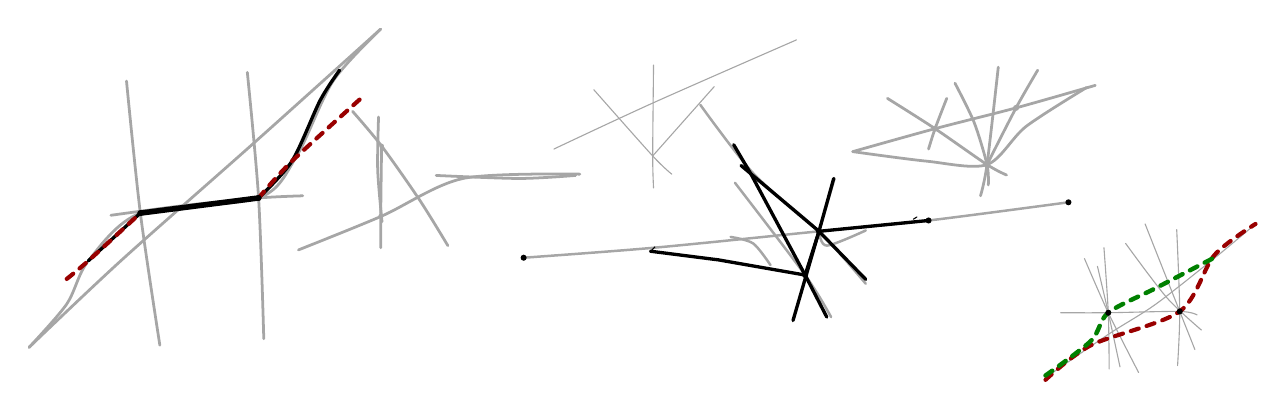
\begin{tikzpicture}[x=.55cm,y=-.55cm,line cap=round,line join=round,g/.style={olive!80!yellow,line width=1.7pt},r/.style={orange!80!brown,line width=1.8pt},w/.style={red!60!black,line width=1.5pt},b/.style={blue!60!black,line width=1.4pt},p/.style={gray!70,thin},k/.style={black,line width=1.2pt},every node/.style={font=\scriptsize}]
% Five local pencil/ink constructions, with red and green dashed alterations.
\draw[p,line width=1pt] plot[smooth] coordinates {(.48,8.3) (2.6,6.3) (5.65,3.6) (8.6,.95)};
\draw[p,line width=1pt] plot[smooth] coordinates {(.48,8.3) (1.35,7.3) (1.85,6.3) (3.05,5.2) (5.78,4.85) (6.65,3.9) (7.5,2.15) (8.6,.95)};
\draw[p,line width=1pt] plot[smooth] coordinates {(2.73,2.15) (3.05,5.2) (3.5,8.25)};
\draw[p,line width=1pt] plot[smooth] coordinates {(5.52,1.95) (5.78,4.85) (5.9,8.1)};
\draw[p,line width=1pt] plot[smooth] coordinates {(2.37,5.25) (4.1,5.02) (5.78,4.85) (6.8,4.8)};
\draw[p,line width=1pt] plot[smooth] coordinates {(6.7,6.05) (8.62,5.27) (10.5,4.4) (13.2,4.3)};
\draw[p,line width=1pt] plot[smooth] coordinates {(7.95,2.85) (8.62,3.65) (9.5,4.9) (10.15,5.95)};
\draw[p,line width=1pt] plot[smooth] coordinates {(8.62,3.65) (8.6,5.27) (8.6,6.0)};
\draw[p,line width=1pt] plot[smooth] coordinates {(8.55,2.98) (8.53,4.2) (8.63,5.4)};
\draw[p,line width=1pt] plot[smooth] coordinates {(9.88,4.33) (11.8,4.4) (13.1,4.33)};
\draw[k,line width=2pt] plot[smooth] coordinates {(3.05,5.2) (5.78,4.85)};
\draw[k] plot[smooth] coordinates {(1.85,6.3) (3.05,5.2)};
\draw[k] plot[smooth] coordinates {(5.78,4.85) (6.55,4.0) (7.2,2.6) (7.65,1.9)};
\draw[w,dashed] plot[smooth] coordinates {(1.35,6.72) (1.85,6.3) (3.05,5.2)};
\draw[w,dashed] plot[smooth] coordinates {(5.78,4.85) (6.55,4.0) (8.2,2.5)};
\fill[k] (3.05,5.2) circle (.07);
\fill[k] (5.78,4.85) circle (.07);
\fill[p] (8.62,3.65) circle (.055);
\fill[p] (8.6,5.27) circle (.055);
% Small upper-central crossing.
\draw[p] plot[smooth] coordinates {(12.6,3.72) (14.9,2.65) (18.2,1.2)};
\draw[p] plot[smooth] coordinates {(13.52,2.35) (14.88,3.88) (15.32,4.3)};
\draw[p] plot[smooth] coordinates {(14.9,1.78) (14.88,3.88) (14.9,4.62)};
\draw[p] plot[smooth] coordinates {(14.88,3.88) (16.3,2.28)};
% Central angular local detours.
\draw[p,line width=.9pt] plot[smooth] coordinates {(11.9,6.23) (14.9,6.0) (18.72,5.62) (21.25,5.37) (24.48,4.95)};
\draw[p,line width=.9pt] plot[smooth] coordinates {(15.98,2.7) (17.22,4.3) (18.72,5.62) (19.8,6.83)};
\draw[p,line width=.9pt] plot[smooth] coordinates {(16.78,4.5) (18.4,6.63) (19.0,7.6)};
\draw[p,line width=.9pt] plot[smooth] coordinates {(18.4,6.63) (18.72,5.62) (19.08,4.4)};
\draw[p,line width=.9pt] plot[smooth] coordinates {(16.68,5.75) (17.2,5.9) (17.6,6.4)};
\draw[p,line width=.9pt] plot[smooth] coordinates {(18.72,5.62) (18.9,5.95) (19.8,5.6)};
\draw[k] (14.83,6.08)--(16.4,6.28)--(18.4,6.63)--(18.72,5.62)--(21.25,5.37);
\draw[k] (16.75,3.62)--(17.15,4.3)--(18.4,6.63)--(18.9,7.6);
\draw[k] (16.92,4.1)--(18.72,5.62)--(19.8,6.73);
\draw[k] (19.06,4.4)--(18.72,5.62)--(18.12,7.68);
\fill[k] (11.9,6.23) circle (.07);
\fill[k] (18.4,6.63) circle (.07);
\fill[k] (18.72,5.62) circle (.07);
\fill[k] (21.25,5.37) circle (.07);
\fill[k] (24.48,4.95) circle (.07);
\draw[k,thin] (14.82,6.1)--(14.93,5.98);
\draw[k,thin] (20.9,5.34)--(20.98,5.29);
% Upper-right fan through three marked points.
\draw[p,line width=1pt] plot[smooth] coordinates {(19.5,3.78) (21.4,3.25) (23.27,2.77) (25.1,2.25)};
\draw[p,line width=1pt] plot[smooth] coordinates {(20.3,2.55) (21.4,3.25) (22.6,4.08) (23.05,4.32)};
\draw[p,line width=1pt] plot[smooth] coordinates {(21.67,2.55) (21.4,3.25) (21.25,3.72)};
\draw[p,line width=1pt] plot[smooth] coordinates {(21.86,2.2) (22.3,3.1) (22.6,4.08) (22.63,4.55)};
\draw[p,line width=1pt] plot[smooth] coordinates {(22.86,1.83) (22.6,4.08) (22.45,4.8)};
\draw[p,line width=1pt] plot[smooth] coordinates {(23.77,1.9) (23.27,2.77) (22.6,4.08)};
\draw[p,line width=1pt] plot[smooth] coordinates {(19.5,3.78) (21.2,4.0) (22.6,4.08) (23.5,3.2) (24.9,2.3)};
\fill[p] (21.4,3.25) circle (.07);
\fill[p] (22.6,4.08) circle (.07);
\fill[p] (23.27,2.77) circle (.07);
% Lower-right two-point sketch, coloured dashed paths.
\draw[p] plot[smooth] coordinates {(23.95,9.0) (25.4,8.0) (26.5,7.3) (27.9,6.2) (28.8,5.45)};
\draw[p] plot[smooth] coordinates {(24.3,7.5) (25.4,7.5) (27.05,7.47) (27.45,7.55)};
\draw[p] plot[smooth] coordinates {(24.85,6.25) (25.4,7.5) (26.1,8.88)};
\draw[p] plot[smooth] coordinates {(25.3,6.0) (25.4,7.5) (25.42,8.8)};
\draw[p] plot[smooth] coordinates {(26.25,5.45) (27.05,7.47) (27.4,8.35)};
\draw[p] plot[smooth] coordinates {(26.98,5.58) (27.05,7.47) (27.0,8.72)};
\draw[p] plot[smooth] coordinates {(25.8,5.9) (26.75,7.15) (27.55,7.9)};
\draw[p] plot[smooth] coordinates {(25.15,6.43) (25.4,7.5) (25.67,8.75)};
\draw[w,dashed] plot[smooth] coordinates {(23.95,9.05) (25.0,8.25) (27.05,7.47) (27.85,6.17) (28.8,5.45)};
\draw[green!50!black,dashed,line width=1.6pt] plot[smooth] coordinates {(23.95,8.95) (25.0,8.15) (25.4,7.5) (26.5,6.93) (27.9,6.2)};
\fill[k] (25.4,7.5) circle (.07);
\fill[k] (27.05,7.47) circle (.07);
\end{tikzpicture}}
{\ttfamily\unsure{***}\quad\unsure{CRAY2}\quad0025\quad I}
{\scriptsize\begin{tabular}{l}
\texttt{\ \ \ \ \ \ \ \ \ \ \ 00000000\ \ \ \ \ \ 00000000\ \ \ \ \ \ 00000000\ \ \ \ \ \ 00000000}\\
\texttt{\ \ \ \ \ \ \ \ \ 0000000000\ \ \ \ 0000000000\ \ \ \ 0000000000\ \ \ \ 0000000000}\\
\texttt{\ \ \ \ \ \ \ 00\ \ \ \ \ \ 0000\ \ 00\ \ \ \ \ \ 0000\ \ 00\ \ \ \ \ \ 0000\ \ 00\ \ \ \ \ \ 0000}\\
\texttt{\ \ \ \ \ \ 00\ \ \ \ \ 00\ 00\ \ 00\ \ \ \ \ 00\ 00\ \ 00\ \ \ \ \ 00\ 00\ \ 00\ \ \ \ \ 00\ 00}\\
\texttt{\ \ \ \ \ 00\ \ \ \ 00\ \ 00\ \ 00\ \ \ \ 00\ \ 00\ \ 00\ \ \ \ 00\ \ 00\ \ 00\ \ \ \ 00\ \ 00}\\
\texttt{\ \ \ \ 00\ \ \ 00\ \ \ 00\ \ 00\ \ \ 00\ \ \ 00\ \ 00\ \ \ 00\ \ \ 00\ \ 00\ \ \ 00\ \ \ 00}\\
\texttt{\ \ \ 00\ \ 00\ \ \ \ 00\ \ 00\ \ 00\ \ \ \ 00\ \ 00\ \ 00\ \ \ \ 00\ \ 00\ \ 00\ \ \ \ 00}\\
\texttt{\ \ 00\ 00\ \ \ \ \ 00\ \ 00\ 00\ \ \ \ \ 00\ \ 00\ 00\ \ \ \ \ 00\ \ 00\ 00\ \ \ \ \ 00}\\
\texttt{\ 0000\ \ \ \ \ \ 00\ \ 0000\ \ \ \ \ \ 00\ \ 0000\ \ \ \ \ \ 00\ \ 0000\ \ \ \ \ \ 00}\\
\texttt{000\ \ \ \ \ \ \ 00\ \ 000\ \ \ \ \ \ \ 00\ \ 000\ \ \ \ \ \ \ 00\ \ 000\ \ \ \ \ \ \ 00}\\
\texttt{0000000000\ \ \ \ 0000000000\ \ \ \ 0000000000\ \ \ \ 0000000000}\\
\texttt{00000000\ \ \ \ \ \ 00000000\ \ \ \ \ \ 00000000\ \ \ \ \ \ 00000000}\\
\texttt{}\\
\texttt{\ CCCCCCCCCC\ \ \ RRRRRRRRRRR\ \ \ AAAAAAAAAA\ \ \ YY\ \ \ \ \ \ \ \ YY\ \ \ 2222222222}\\
\texttt{CCCCCCCCCCCC\ \ RRRRRRRRRRRR\ AAAAAAAAAAAA\ \ YY\ \ \ \ \ \ \ \ YY\ \ 222222222222}\\
\texttt{CC\ \ \ \ \ \ \ \ CC\ \ RR\ \ \ \ \ \ \ \ RR\ AA\ \ \ \ \ \ \ \ AA\ \ YY\ \ \ \ \ \ YY\ \ \ 22\ \ \ \ \ \ \ \ 22}\\
\texttt{CC\ \ \ \ \ \ \ \ \ \ \ \ RR\ \ \ \ \ \ \ \ RR\ AA\ \ \ \ \ \ \ \ AA\ \ \ YY\ \ \ \ YY\ \ \ \ \ \ \ \ \ \ \ \ \ 22}\\
\texttt{CC\ \ \ \ \ \ \ \ \ \ \ \ RR\ \ \ \ \ \ \ \ RR\ AA\ \ \ \ \ \ \ \ AA\ \ \ \ YY\ \ YY\ \ \ \ \ \ \ \ \ \ \ \ \ \ 22}\\
\texttt{CC\ \ \ \ \ \ \ \ \ \ \ \ RRRRRRRRRRRR\ AAAAAAAAAAAA\ \ \ \ \ YYYY\ \ \ \ \ \ \ \ \ \ \ \ \ \ 22}\\
\texttt{CC\ \ \ \ \ \ \ \ \ \ \ \ RRRRRRRRRRR\ \ AAAAAAAAAAAA\ \ \ \ \ \ YY\ \ \ \ \ \ \ \ \ \ \ \ \ \ 22}\\
\texttt{CC\ \ \ \ \ \ \ \ \ \ \ \ RR\ \ \ \ RR\ \ \ \ \ AA\ \ \ \ \ \ \ \ AA\ \ \ \ \ \ YY\ \ \ \ \ \ \ \ \ \ \ \ \ 22}\\
\texttt{CC\ \ \ \ \ \ \ \ \ \ \ \ RR\ \ \ \ \ RR\ \ \ \ AA\ \ \ \ \ \ \ \ AA\ \ \ \ \ \ YY\ \ \ \ \ \ \ \ \ \ \ \ 22}\\
\texttt{CC\ \ \ \ \ \ \ \ CC\ \ RR\ \ \ \ \ \ RR\ \ \ AA\ \ \ \ \ \ \ \ AA\ \ \ \ \ \ YY\ \ \ \ \ \ \ \ \ \ \ 22}\\
\texttt{CCCCCCCCCCCC\ \ RR\ \ \ \ \ \ \ RR\ \ AA\ \ \ \ \ \ \ \ AA\ \ \ \ \ \ YY\ \ \ \ \ \ \ \ \ \ 222222222222}\\
\texttt{\ CCCCCCCCCC\ \ \ RR\ \ \ \ \ \ \ \ RR\ AA\ \ \ \ \ \ \ \ AA\ \ \ \ \ \ YY\ \ \ \ \ \ \ \ \ \ 222222222222}\\
\end{tabular}}
{\ttfamily ****A\quad\unsure{END|FND}\quad JOB\quad25\quad CRAY2\quad ROOM\quad 9.03.23 AM 19 AUG 82\quad R6.PR1\quad SYS JES2\quad JOB\quad25\quad END\quad A****}\\
{\ttfamily ****A\quad\unsure{END|FND}\quad JOB\quad25\quad CRAY2\quad ROOM\quad 9.03.23 AM 19 AUG 82\quad R6.PR1\quad SYS JES2\quad JOB\quad25\quad END\quad A****}\\
{\ttfamily ****A\quad\unsure{END|FND}\quad JOB\quad25\quad CRAY2\quad ROOM\quad 9.03.23 AM 19 AUG 82\quad R6.PR1\quad SYS JES2\quad JOB\quad25\quad END\quad A****}\\
{\ttfamily ****A\quad\unsure{END|FND}\quad JOB\quad25\quad CRAY2\quad ROOM\quad 9.03.23 AM 19 AUG 82\quad R6.PR1\quad SYS JES2\quad JOB\quad25\quad END\quad A****}\\
{\ttfamily ****A\quad\unsure{END|FND}\quad JOB\quad25\quad CRAY2\quad ROOM\quad 9.03.23 AM 19 AUG 82\quad R6.PR1\quad SYS JES2\quad JOB\quad25\quad END\quad A****}\\
{\ttfamily ****A\quad\unsure{END|FND}\quad JOB\quad25\quad CRAY2\quad ROOM\quad 9.03.23 AM 19 AUG 82\quad R6.PR1\quad SYS JES2\quad JOB\quad25\quad END\quad A****}\\
\margin{\mspage{143}}

\scanpage{145}
\begin{center}\texttt{D A T A S E T S\quad P I C T U R E S}\end{center}
% E02: printed listing table, including its star boundaries.
\diagram{\[
\begin{array}{c@{\;}l@{\;}c@{\;}l@{\;}c@{\;}c@{\;}c@{\;}c@{\;}c@{\;}r@{\;}c@{\;}r@{\;}c@{\;}l@{\;}c@{\;}l@{\;}c@{\;}l@{\;}c@{\;}l@{\;}c}
\multicolumn{21}{c}{\texttt{******************************************************************************************************************}}\\
*& &*& &*& &*& &*& &*& &*& &*& &*& &*& &*\\
*&\texttt{DDNAME}&*&\texttt{DESTINATION}&*&\texttt{CLASS}&*&\texttt{COPIES}&*&\texttt{RECORDS-NB}&*&\texttt{BYTES-NB}&*&\texttt{FORM}&*&\texttt{FCB}&*&\texttt{UCS}&*&\texttt{SPIN\ HOLD}&*\\
*& &*& &*& &*& &*& &*& &*& &*& &*& &*& &*\\
\multicolumn{21}{c}{\texttt{******************************************************************************************************************}}\\
*& &*& &*& &*& &*& &*& &*& &*& &*& &*& &*\\
*&\texttt{SYSMSG}&*&\texttt{CNU\qquad M06}&*&\texttt{A}&*&1&*&67&*&\texttt{3,893}&*&\texttt{STD.}&*&\texttt{****}&*&\texttt{****}&*& &*\\
\multicolumn{21}{c}{\texttt{******************************************************************************************************************}}
\end{array}
\]}

\deleted{$A B C D E F G$}\\
\deleted{$A B C E D$} $G F$
\diagram{\begin{tikzcd}[ampersand replacement=\&,column sep=.35em,row sep=.9em]
{} \& {} \& {} \& {} \& D\arrow[dr] \& {} \& E\arrow[dl] \& {} \& F\arrow[dr] \& {} \& G\arrow[dl] \& {} \& {} \& {} \& {}\\
{} \& {} \& {} \& {} \& {} \& DE\arrow[drr] \& {} \& {} \& {} \& FG\arrow[dll]\arrow[rrr,dash] \& {} \& {} \& ABC\underbrace{DE}\underbrace{FG} \& {} \& 1'\\
{} \& {} \& {} \& {} \& {} \& {} \& {} \& DG\arrow[dl]\arrow[rrrrr,dash] \& {} \& {} \& {} \& {} \& ABCE\uline{D}\underbrace{GF} \& {} \& 2'\\
{} \& {} \& {} \& {} \& {} \& {} \& EG\arrow[dl]\arrow[rrrrrr,dash] \& {} \& {} \& {} \& {} \& {} \& ABCE\uline{GD}F \& {} \& 3'\\
{} \& {} \& {} \& {} \& {} \& \unsure{CG}\arrow[dl]\arrow[rrrrrrr,dash] \& {} \& {} \& {} \& {} \& {} \& {} \& AB\underbrace{CGE}DF \& {} \& 4'\\
{} \& {} \& {} \& {} \& BG\arrow[dl]\arrow[dr]\arrow[rrrrrrrr,dash] \& {} \& {} \& {} \& {} \& {} \& {} \& {} \& AB\underbrace{GC}EDF \& {} \& 5'\\
{} \& {} \& {} \& AG\arrow[d] \& {} \& {}\arrow[dr]\arrow[rrrrrrr,dash] \& {} \& {} \& {} \& {} \& {} \& {} \& A\underbrace{GB}CEDF \& {} \& 6'\\
{} \& {} \& {} \& {}\arrow[d] \& {} \& {} \& {}\arrow[dl,line width=1.7pt]\arrow[dr,line width=1.7pt]\arrow[rrrrrr,dash] \& {} \& {} \& {} \& {} \& {} \& \textcircled{\scriptsize $\unsure{GA|AG}$}\uline{CB}EDF \& {} \& 7'\\
{} \& {} \& {} \& {}\arrow[d] \& {} \& {}\arrow[dr,line width=1.7pt] \& {} \& {}\arrow[dl,line width=1.7pt]\arrow[dr,line width=1.7pt]\arrow[rrrrr,dash] \& {} \& {} \& {} \& {} \& \textcircled{\scriptsize $AG$}C\uline{EB}DF \& {} \& 8'\\
{} \& {} \& {} \& \unsure{AG}\arrow[d] \& {} \& {} \& {}\arrow[dl,line width=1.7pt]\arrow[dr,line width=1.7pt] \& {} \& {}\arrow[dl,line width=1.7pt]\arrow[dr,line width=1.7pt]\arrow[rrrr,dash] \& {} \& {} \& {} \& \textcircled{\scriptsize $AG$}\uline{EC}D\uline{BF} \& {} \& 9'\\
{} \& {} \& {} \& {}\arrow[dl]\arrow[dr] \& {} \& {}\arrow[dl]\arrow[dr] \& {} \& {} \& {} \& {}\arrow[dl]\arrow[dr] \& {} \& {} \& GAED\unsure{C}FB \& {} \& {}\\
{} \& {} \& {} \& {} \& {} \& {} \& {} \& {} \& {} \& {} \& {} \& {} \& {} \& {} \& {}
\end{tikzcd}}
\figure{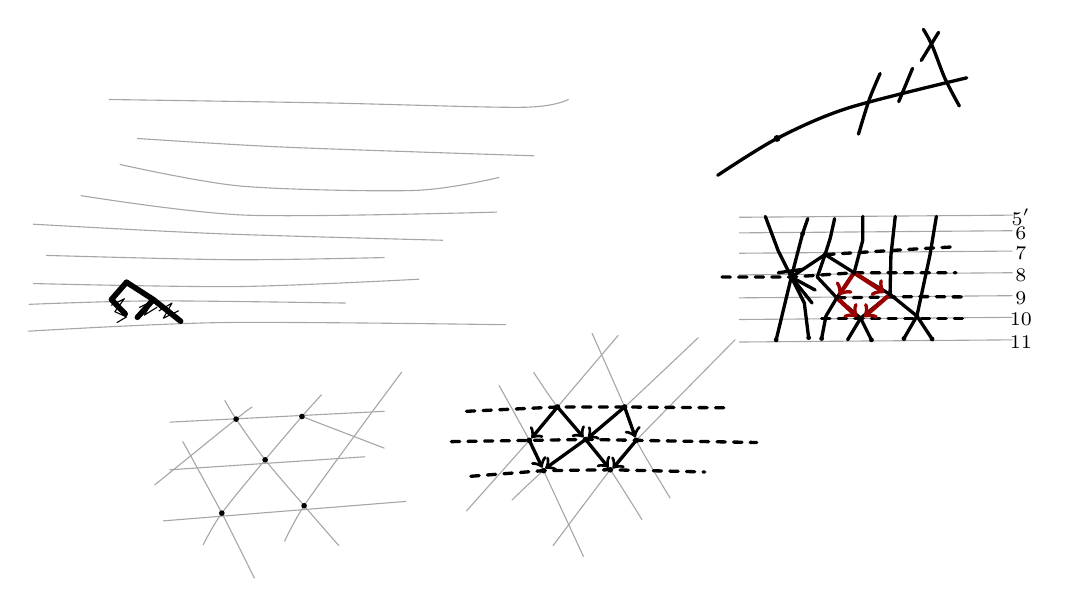
\begin{tikzpicture}[x=.55cm,y=-.55cm,line cap=round,line join=round,g/.style={olive!80!yellow,line width=1.7pt},r/.style={orange!80!brown,line width=1.8pt},w/.style={red!60!black,line width=1.5pt},b/.style={blue!60!black,line width=1.4pt},p/.style={gray!70,thin},k/.style={black,line width=1.2pt},every node/.style={font=\scriptsize}]
% Pencil separators behind the main orders and dark redrawings of lower arrows.
\draw[p] plot[smooth] coordinates {(7.95,8.4) (13.0,8.48) (17.5,8.58) (18.55,8.4)};
\draw[p] plot[smooth] coordinates {(8.6,9.3) (12.0,9.5) (17.75,9.7)};
\draw[p] plot[smooth] coordinates {(8.2,9.9) (11.0,10.4) (15.0,10.5) (16.95,10.2)};
\draw[p] plot[smooth] coordinates {(7.3,10.62) (11.1,11.07) (16.9,11.0)};
\draw[p] plot[smooth] coordinates {(6.2,11.28) (10.5,11.5) (15.65,11.65)};
\draw[p] plot[smooth] coordinates {(6.5,12.0) (10.8,12.1) (14.3,12.05)};
\draw[p] plot[smooth] coordinates {(6.2,12.65) (10.9,12.72) (15.1,12.55)};
\draw[p] plot[smooth] coordinates {(6.1,13.13) (9.0,13.05) (13.4,13.1)};
\draw[p] plot[smooth] coordinates {(6.08,13.75) (10.6,13.55) (17.1,13.6)};
\draw[k,line width=2pt] (8.35,12.62)--(8.0,13.02)--(8.32,13.35);
\draw[k,line width=2pt] (8.35,12.62)--(8.97,13.02)--(8.6,13.43);
\draw[k,line width=2pt] (8.97,13.02)--(9.6,13.52);
\draw[k,thin] (8.0,13.15)--(8.3,13.0)--(8.08,13.3)--(8.35,13.42)--(8.13,13.55);
\draw[k,thin] (8.65,13.2)--(8.96,13.05)--(8.76,13.38)--(9.05,13.2);
\draw[k,thin] (9.1,13.28)--(9.4,13.1)--(9.2,13.45)--(9.55,13.28);
% Upper-right marked line and small crossing.
\draw[k] plot[smooth] coordinates {(22.0,10.15) (23.37,9.3) (25.0,8.6) (27.75,7.9)};
\draw[k] plot[smooth] coordinates {(25.25,9.2) (25.5,8.4) (25.75,7.8)};
\draw[k] plot[smooth] coordinates {(26.18,8.45) (26.5,7.68)};
\draw[k] plot[smooth] coordinates {(26.75,6.78) (26.95,7.15) (27.25,7.92) (27.58,8.55)};
\draw[k] plot[smooth] coordinates {(26.7,7.5) (27.1,6.85)};
\fill[k] (23.37,9.3) circle (.08);
% Middle-right partial grid and darker diagonal paths.
\draw[p] (22.5,11.12)--(28.8,11.069999999999999);
\node at (29.0,11.12) {$5'$};
\draw[p] (22.5,11.48)--(28.8,11.43);
\node at (29.0,11.48) {$6$};
\draw[p] (22.5,11.95)--(28.8,11.899999999999999);
\node at (29.0,11.95) {$7$};
\draw[p] (22.5,12.45)--(28.8,12.399999999999999);
\node at (29.0,12.45) {$8$};
\draw[p] (22.5,12.98)--(28.8,12.93);
\node at (29.0,12.98) {$9$};
\draw[p] (22.5,13.48)--(28.8,13.43);
\node at (29.0,13.48) {$10$};
\draw[p] (22.5,14.0)--(28.8,13.95);
\node at (29.0,14.0) {$11$};
\draw[k] (23.1,11.1)--(23.4,11.9)--(23.7,12.5)--(24.0,13.1)--(24.1,13.9);
\draw[k] (24.08,11.15)--(23.96,11.5)--(23.7,12.5)--(23.35,13.95);
\draw[k] (24.7,11.15)--(24.6,11.6)--(24.48,11.98)--(24.3,12.5)--(24.75,12.98)--(25.3,13.45)--(25.55,13.95);
\draw[k] (25.35,11.1)--(25.35,11.65)--(25.15,12.4)--(24.75,12.98)--(24.5,13.4)--(24.4,13.92);
\draw[k] (26.1,11.1)--(26.0,12.0)--(25.98,12.9)--(25.3,13.45)--(25.0,13.95);
\draw[k] (27.05,11.1)--(26.9,12.0)--(26.6,13.4)--(26.95,13.93);
\draw[k] (23.7,12.5)--(24.48,11.98)--(25.15,12.4)--(25.98,12.9)--(26.6,13.4)--(26.3,13.92);
\draw[k,dashed] (22.1,12.5)--(23.7,12.5)--(25.15,12.4)--(27.5,12.4);
\draw[k,dashed] (24.5,11.98)--(26.6,11.85)--(27.5,11.8);
\draw[k,dashed] (24.75,12.98)--(26.6,12.95)--(27.8,12.96);
\draw[k,dashed] (24.4,13.45)--(25.3,13.45)--(27.65,13.45);
\draw[w,->] (25.15,12.4)--(24.8,12.92);
\draw[w,->] (25.15,12.4)--(25.85,12.86);
\draw[w,->] (24.75,12.98)--(25.22,13.42);
\draw[w,->] (25.98,12.9)--(25.38,13.42);
\fill[k] (23.96,11.5) circle (.055);
\fill[k] (23.7,12.5) circle (.055);
\fill[k] (24.48,11.98) circle (.055);
\fill[k] (25.15,12.4) circle (.055);
\fill[k] (24.75,12.98) circle (.055);
\fill[k] (25.98,12.9) circle (.055);
\fill[k] (25.3,13.45) circle (.055);
\fill[k] (26.6,13.4) circle (.055);
\fill[k] (23.35,13.95) circle (.055);
\fill[k] (24.1,13.9) circle (.055);
\fill[k] (24.4,13.92) circle (.055);
\fill[k] (25.55,13.95) circle (.055);
\fill[k] (26.3,13.92) circle (.055);
\fill[k] (26.95,13.93) circle (.055);
\draw[k] (23.4,12.4)--(23.98,12.32);
\draw[k] (23.7,12.5)--(24.25,12.8);
\draw[k] (23.7,12.5)--(24.18,13.1);
% Bottom middle pencil crossing arrangement.
\draw[p] plot[smooth] coordinates {(9.35,15.85) (14.3,15.6)};
\draw[p] plot[smooth] coordinates {(9.35,16.95) (13.85,16.65)};
\draw[p] plot[smooth] coordinates {(9.2,18.13) (14.8,17.68)};
\draw[p] plot[smooth] coordinates {(9.65,16.3) (10.55,17.95) (11.3,19.45)};
\draw[p] plot[smooth] coordinates {(10.62,15.35) (10.88,15.78) (11.55,16.72) (12.45,17.78) (13.25,18.7)};
\draw[p] plot[smooth] coordinates {(12.85,15.22) (12.4,15.72) (11.55,16.72) (10.55,17.95) (10.12,18.68)};
\draw[p] plot[smooth] coordinates {(14.7,14.7) (13.7,16.05) (12.45,17.78) (12.0,18.6)};
\draw[p] plot[smooth] coordinates {(9.0,17.3) (10.88,15.78) (11.25,15.5)};
\draw[p] plot[smooth] coordinates {(12.4,15.72) (14.3,16.45)};
\fill[k] (10.88,15.78) circle (.065);
\fill[k] (12.4,15.72) circle (.065);
\fill[k] (11.55,16.72) circle (.065);
\fill[k] (10.55,17.95) circle (.065);
\fill[k] (12.45,17.78) circle (.065);
% Bottom-right local arrangement with arrows between three dashed levels.
\draw[p] plot[smooth] coordinates {(16.2,17.9) (17.65,16.27) (18.3,15.5) (19.7,13.85)};
\draw[p] plot[smooth] coordinates {(17.75,14.7) (18.3,15.5) (18.95,16.25) (19.52,16.95) (20.25,18.1)};
\draw[p] plot[smooth] coordinates {(19.1,13.8) (19.85,15.5) (20.12,16.27) (20.9,17.6)};
\draw[p] plot[smooth] coordinates {(16.95,15.0) (17.65,16.27) (17.98,16.97) (18.9,18.95)};
\draw[p] plot[smooth] coordinates {(17.25,17.65) (17.98,16.97) (18.95,16.25) (19.85,15.5) (21.55,13.9)};
\draw[p] plot[smooth] coordinates {(18.2,18.7) (19.52,16.95) (20.12,16.27) (22.4,13.95)};
\draw[k,dashed] (16.2,15.6)--(18.3,15.5)--(19.85,15.5)--(22.25,15.52);
\draw[k,dashed] (15.85,16.3)--(18.95,16.25)--(20.12,16.27)--(22.9,16.32);
\draw[k,dashed] (16.3,17.1)--(17.98,16.97)--(19.52,16.95)--(21.7,17.0);
\draw[k,->] (18.3,15.5)--(17.7,16.22);
\draw[k,->] (18.3,15.5)--(18.9,16.2);
\draw[k,->] (19.85,15.5)--(19.0,16.22);
\draw[k,->] (19.85,15.5)--(20.1,16.2);
\draw[k,->] (17.65,16.27)--(17.95,16.9);
\draw[k,->] (18.95,16.25)--(18.02,16.92);
\draw[k,->] (18.95,16.25)--(19.48,16.9);
\draw[k,->] (20.12,16.27)--(19.58,16.92);
\fill[k] (18.3,15.5) circle (.065);
\fill[k] (19.85,15.5) circle (.065);
\fill[k] (17.65,16.27) circle (.065);
\fill[k] (18.95,16.25) circle (.065);
\fill[k] (20.12,16.27) circle (.065);
\fill[k] (17.98,16.97) circle (.065);
\fill[k] (19.52,16.95) circle (.065);
\end{tikzpicture}}
\diagram{\begin{tikzcd}[ampersand replacement=\&,column sep=.8em,row sep=1em]
\bullet\arrow[dr]\&{}\&\bullet\arrow[dl]\&\bullet\arrow[dr]\&{}\&\bullet\arrow[dl]\\
{}\&{}\arrow[drr]\&{}\&{}\&{}\arrow[dl]\&{}\\
{}\&{}\&{}\&{}\arrow[dl]\&{}\&{}\\
{}\&{}\&{}\arrow[dl]\&{}\&{}\&{}\\
{}\&{}\&{}\&{}\&{}\&{}
\end{tikzcd}}
\margin{\mspage{144}}

\scanpage{146}
\figure{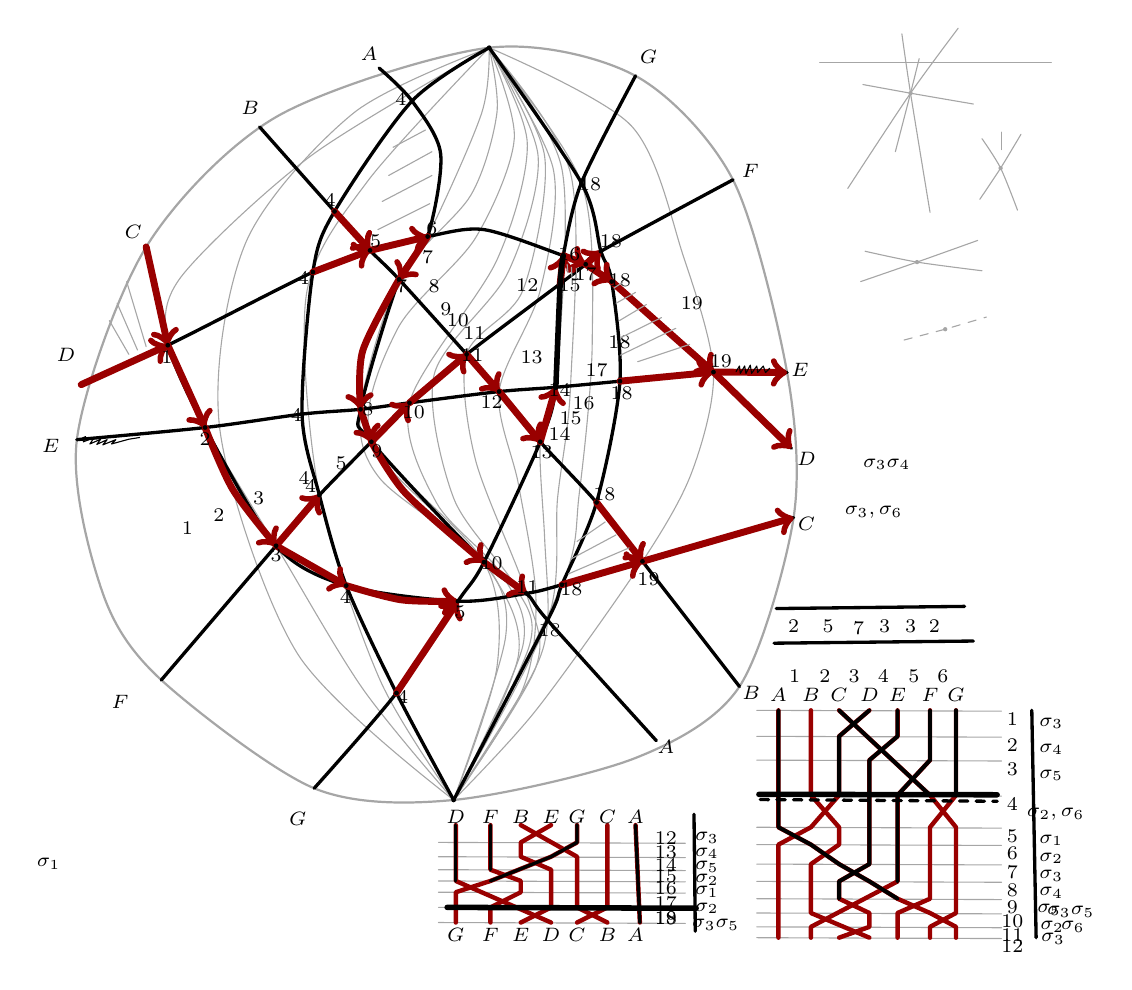
\begin{tikzpicture}[x=.55cm,y=-.55cm,line cap=round,line join=round,g/.style={olive!80!yellow,line width=1.7pt},r/.style={orange!80!brown,line width=1.8pt},w/.style={red!60!black,line width=1.5pt},b/.style={blue!60!black,line width=1.4pt},p/.style={gray!70,thin},k/.style={black,line width=1.2pt},every node/.style={font=\scriptsize}]
% Main large oval and pencil family; individual numbered intersections are retained.
\draw[p,line width=.8pt] plot[smooth cycle] coordinates {(15.92,1.7) (11.0,3.3) (8.0,6.3) (6.4,10.75) (7.0,14.3) (8.35,16.3) (11.88,18.8) (15.1,19.07) (19.3,18.1) (21.7,16.45) (22.95,12.55) (22.8,9.2) (21.55,4.75) (19.3,2.35)};
\draw[p] plot[smooth] coordinates {(15.92,1.7) (12.8,3.2) (10.3,6.2) (9.7,10.5) (11.5,15.7) (15.1,19.07)};
\draw[p] plot[smooth] coordinates {(15.92,1.7) (11.8,4.2) (8.8,7.0) (8.5,8.57) (9.36,10.47) (11.0,13.2) (13.0,16.5) (15.1,19.07)};
\draw[p] plot[smooth] coordinates {(15.92,1.7) (13.1,4.8) (11.7,7.4) (12.0,12.03) (13.4,16.3) (15.1,19.07)};
\draw[p] plot[smooth] coordinates {(15.92,1.7) (15.75,3.2) (14.5,6.06) (13.0,8.8) (13.2,10.8) (15.8,13.58) (16.1,16.0) (15.1,19.07)};
\draw[p] plot[smooth] coordinates {(15.92,1.7) (16.1,3.2) (15.5,5.1) (13.84,7.05) (12.95,10.05) (13.4,11.65) (15.8,13.58) (16.3,15.3) (15.1,19.07)};
\draw[p] plot[smooth] coordinates {(15.92,1.7) (16.5,3.8) (15.6,6.1) (13.8,8.2) (13.2,10.8) (15.8,13.58) (16.6,15.7) (15.1,19.07)};
\draw[p] plot[smooth] coordinates {(15.92,1.7) (16.8,3.9) (16.1,6.6) (14.08,9.9) (14.7,12.2) (16.2,13.85) (16.7,15.5) (15.1,19.07)};
\draw[p] plot[smooth] coordinates {(15.92,1.7) (17.05,4.2) (16.35,6.9) (14.65,9.25) (15.1,12.1) (16.5,14.1) (16.85,15.5) (15.1,19.07)};
\draw[p] plot[smooth] coordinates {(15.92,1.7) (17.2,4.2) (16.7,7.3) (15.4,8.78) (15.6,11.2) (16.78,14.3) (17.0,16.0) (15.1,19.07)};
\draw[p] plot[smooth] coordinates {(15.92,1.7) (17.4,4.5) (17.1,7.3) (16.15,9.64) (16.6,11.8) (17.0,14.4) (16.7,16.5) (15.1,19.07)};
\draw[p] plot[smooth] coordinates {(15.92,1.7) (17.6,4.5) (17.46,9.54) (17.1,10.8) (17.2,13.0) (17.27,14.92) (16.9,16.2) (15.1,19.07)};
\draw[p] plot[smooth] coordinates {(15.92,1.7) (17.8,4.6) (17.8,9.5) (17.5,12.1) (17.27,14.92) (15.1,19.07)};
\draw[p] plot[smooth] coordinates {(15.92,1.7) (18.05,4.82) (18.3,8.5) (18.0,12.0) (17.6,14.1) (15.1,19.07)};
\draw[p] plot[smooth] coordinates {(15.92,1.7) (19.2,3.5) (20.4,6.5) (21.1,9.19) (20.6,11.5) (19.46,13.56) (17.0,17.0) (15.1,19.07)};
\draw[k] plot[smooth] coordinates {(15.92,1.7) (14.14,2.93) (12.35,5.48) (11.85,6.88) (11.6,10.16) (12.0,12.03) (12.62,14.12) (13.78,16.6) (15.1,19.07)};
\draw[k] plot[smooth] coordinates {(15.92,1.7) (18.05,4.82) (18.5,6.4) (18.75,7.1) (18.94,9.4) (18.4,12.2) (17.6,14.1) (17.27,14.92) (15.1,19.07)};
\draw[k] plot[smooth] coordinates {(13.38,2.17) (14.14,2.93) (14.8,4.15) (14.5,6.06) (13.84,7.05) (12.95,10.05) (13.2,10.8) (15.8,13.58) (16.78,14.3) (17.27,14.92) (19.78,17.7)};
\draw[k] plot[smooth] coordinates {(10.62,3.53) (12.35,5.48) (13.17,6.38) (13.84,7.05) (15.4,8.78) (16.15,9.64) (17.1,10.8) (18.4,12.2) (19.46,13.56) (21.7,16.45)};
\draw[k] plot[smooth] coordinates {(8.0,6.3) (8.5,8.57) (9.36,10.47) (11.0,13.2) (12.62,14.12) (15.2,14.48) (16.78,14.3) (17.6,14.1) (19.46,13.56) (22.95,12.55)};
\draw[k] plot[smooth] coordinates {(6.5,9.48) (8.5,8.57) (11.85,6.88) (13.17,6.38) (14.5,6.06) (15.8,5.9) (17.63,6.5) (18.15,6.7) (18.75,7.1) (21.1,9.19) (22.9,10.95)};
\draw[k] plot[smooth] coordinates {(6.4,10.75) (9.36,10.47) (11.6,10.16) (12.95,10.05) (14.08,9.9) (16.15,9.64) (17.46,9.54) (18.94,9.4) (21.1,9.19) (22.8,9.2)};
\draw[k] plot[smooth] coordinates {(8.35,16.3) (11.0,13.2) (12.0,12.03) (13.2,10.8) (14.08,9.9) (15.4,8.78) (17.56,7.15) (18.15,6.7) (18.5,6.4) (21.55,4.75)};
\draw[k] plot[smooth] coordinates {(11.88,18.8) (13.78,16.6) (15.2,14.48) (15.8,13.58) (17.1,10.8) (17.46,9.54) (17.56,7.15) (17.63,6.5) (18.05,4.82) (19.3,2.35)};
\draw[w,->,line width=2.5pt] plot[smooth] coordinates {(8.0,6.3) (8.5,8.57)};
\draw[w,->,line width=2.5pt] plot[smooth] coordinates {(6.5,9.48) (8.5,8.57)};
\draw[w,->,line width=2.5pt] plot[smooth] coordinates {(8.5,8.57) (9.36,10.47)};
\draw[w,->,line width=2.5pt] plot[smooth] coordinates {(9.36,10.47) (10.0,11.9) (11.0,13.2)};
\draw[w,->,line width=2.5pt] plot[smooth] coordinates {(11.0,13.2) (12.0,12.03)};
\draw[w,->,line width=2.5pt] plot[smooth] coordinates {(11.0,13.2) (12.62,14.12)};
\draw[w,->,line width=2.5pt] plot[smooth] coordinates {(12.62,14.12) (13.9,14.45) (15.2,14.48)};
\draw[w,->,line width=2.5pt] plot[smooth] coordinates {(13.78,16.6) (15.2,14.48)};
\draw[w,->,line width=2.5pt] plot[smooth] coordinates {(12.35,5.48) (13.17,6.38)};
\draw[w,->,line width=2.5pt] plot[smooth] coordinates {(11.85,6.88) (13.17,6.38)};
\draw[w,->,line width=2.5pt] plot[smooth] coordinates {(13.17,6.38) (14.5,6.06)};
\draw[w,->,line width=2.5pt] plot[smooth] coordinates {(14.5,6.06) (13.84,7.05)};
\draw[w,->,line width=2.5pt] plot[smooth] coordinates {(13.84,7.05) (13.0,8.7) (12.95,10.05)};
\draw[w,->,line width=2.5pt] plot[smooth] coordinates {(12.95,10.05) (13.2,10.8)};
\draw[w,->,line width=2.5pt] plot[smooth] coordinates {(13.2,10.8) (14.08,9.9)};
\draw[w,->,line width=2.5pt] plot[smooth] coordinates {(14.08,9.9) (15.4,8.78)};
\draw[w,->,line width=2.5pt] plot[smooth] coordinates {(15.4,8.78) (16.15,9.64)};
\draw[w,->,line width=2.5pt] plot[smooth] coordinates {(16.15,9.64) (17.1,10.8)};
\draw[w,->,line width=2.5pt] plot[smooth] coordinates {(17.1,10.8) (17.46,9.54)};
\draw[w,->,line width=2.5pt] plot[smooth] coordinates {(13.2,10.8) (14.0,12.0) (15.8,13.58)};
\draw[w,->,line width=2.5pt] plot[smooth] coordinates {(15.8,13.58) (16.78,14.3)};
\draw[w,->,line width=2.5pt] plot[smooth] coordinates {(17.6,14.1) (19.46,13.56)};
\draw[w,->,line width=2.5pt] plot[smooth] coordinates {(18.4,12.2) (19.46,13.56)};
\draw[w,->,line width=2.5pt] plot[smooth] coordinates {(19.46,13.56) (22.95,12.55)};
\draw[w,->,line width=2.5pt] plot[smooth] coordinates {(17.56,7.15) (17.63,6.5)};
\draw[w,->,line width=2.5pt] plot[smooth] coordinates {(17.63,6.5) (18.15,6.7)};
\draw[w,->,line width=2.5pt] plot[smooth] coordinates {(18.15,6.7) (18.5,6.4)};
\draw[w,->,line width=2.5pt] plot[smooth] coordinates {(18.15,6.7) (18.75,7.1)};
\draw[w,->,line width=2.5pt] plot[smooth] coordinates {(18.75,7.1) (21.1,9.19)};
\draw[w,->,line width=2.5pt] plot[smooth] coordinates {(18.94,9.4) (21.1,9.19)};
\draw[w,->,line width=2.5pt] plot[smooth] coordinates {(21.1,9.19) (22.8,9.2)};
\draw[w,->,line width=2.5pt] plot[smooth] coordinates {(21.1,9.19) (22.9,10.95)};
\draw[k,line width=2pt] plot[smooth] coordinates {(17.46,9.54) (17.56,7.15) (17.63,6.5)};
\fill[k] (15.92,1.7) circle (.055);
\fill[k] (15.1,19.07) circle (.055);
\fill[k] (14.14,2.93) circle (.055);
\fill[k] (12.35,5.48) circle (.055);
\fill[k] (11.85,6.88) circle (.055);
\fill[k] (11.6,10.16) circle (.055);
\fill[k] (12.0,12.03) circle (.055);
\fill[k] (12.62,14.12) circle (.055);
\fill[k] (13.78,16.6) circle (.055);
\fill[k] (18.05,4.82) circle (.055);
\fill[k] (18.5,6.4) circle (.055);
\fill[k] (18.75,7.1) circle (.055);
\fill[k] (18.94,9.4) circle (.055);
\fill[k] (18.4,12.2) circle (.055);
\fill[k] (17.6,14.1) circle (.055);
\fill[k] (17.27,14.92) circle (.055);
\fill[k] (14.5,6.06) circle (.055);
\fill[k] (13.84,7.05) circle (.055);
\fill[k] (12.95,10.05) circle (.055);
\fill[k] (13.2,10.8) circle (.055);
\fill[k] (15.8,13.58) circle (.055);
\fill[k] (16.78,14.3) circle (.055);
\fill[k] (13.17,6.38) circle (.055);
\fill[k] (15.4,8.78) circle (.055);
\fill[k] (16.15,9.64) circle (.055);
\fill[k] (17.1,10.8) circle (.055);
\fill[k] (19.46,13.56) circle (.055);
\fill[k] (8.5,8.57) circle (.055);
\fill[k] (9.36,10.47) circle (.055);
\fill[k] (11.0,13.2) circle (.055);
\fill[k] (15.2,14.48) circle (.055);
\fill[k] (17.63,6.5) circle (.055);
\fill[k] (18.15,6.7) circle (.055);
\fill[k] (21.1,9.19) circle (.055);
\fill[k] (14.08,9.9) circle (.055);
\fill[k] (17.46,9.54) circle (.055);
\fill[k] (17.56,7.15) circle (.055);
\node at (13.15,1.85) {$A$};
\node at (10.4,3.1) {$B$};
\node at (7.7,5.95) {$C$};
\node at (6.15,8.8) {$D$};
\node at (5.8,10.9) {$E$};
\node at (7.4,16.8) {$F$};
\node at (11.5,19.5) {$G$};
\node at (19.6,1.92) {$G$};
\node at (21.95,4.55) {$F$};
\node at (23.1,9.15) {$E$};
\node at (23.25,11.2) {$D$};
\node at (23.25,12.7) {$C$};
\node at (21.97,16.6) {$B$};
\node at (20.0,17.85) {$A$};
\node at (5.75,20.55) {$\sigma_1$};
\node at (8.48,8.85) {$1$};
\node at (9.36,10.73) {$2$};
\node at (11.0,13.43) {$3$};
\node at (12.6,14.38) {$4$};
\node at (15.25,14.73) {$5$};
\node at (14.6,5.88) {$6$};
\node at (13.9,7.2) {$7$};
\node at (13.12,10.05) {$8$};
\node at (13.33,11.02) {$9$};
\node at (14.18,10.12) {$10$};
\node at (15.53,8.8) {$11$};
\node at (15.98,9.88) {$12$};
\node at (17.13,11.03) {$13$};
\node at (17.55,9.6) {$14$};
\node at (17.78,7.18) {$15$};
\node at (17.77,6.47) {$16$};
\node at (18.15,6.94) {$17$};
\node at (18.73,6.17) {$18$};
\node at (18.94,7.07) {$18$};
\node at (18.98,9.68) {$18$};
\node at (18.58,12.0) {$18$};
\node at (17.82,14.2) {$18$};
\node at (17.32,15.15) {$18$};
\node at (18.25,4.85) {$18$};
\node at (21.27,8.95) {$19$};
\node at (19.6,13.98) {$19$};
\node at (15.98,13.6) {$10$};
\node at (16.8,14.16) {$11$};
\node at (13.92,16.7) {$4$};
\node at (12.25,5.23) {$4$};
\node at (11.63,7.02) {$4$};
\node at (11.47,10.18) {$4$};
\node at (11.8,11.83) {$4$};
\node at (13.3,6.17) {$5$};
\node at (13.88,2.88) {$4$};
\node at (8.95,12.8) {$1$};
\node at (9.68,12.5) {$2$};
\node at (10.6,12.1) {$3$};
\node at (11.65,11.65) {$4$};
\node at (12.5,11.3) {$5$};
\node at (14.5,6.53) {$7$};
\node at (14.65,7.2) {$8$};
\node at (14.92,7.75) {$9$};
\node at (15.2,8.0) {$10$};
\node at (15.58,8.3) {$11$};
\node at (16.8,7.18) {$12$};
\node at (16.9,8.85) {$\unsure{13}$};
\node at (17.55,10.63) {$14$};
\node at (17.8,10.25) {$15$};
\node at (18.1,9.9) {$16$};
\node at (18.4,9.15) {$17$};
\node at (18.93,8.5) {$18$};
\node at (20.6,7.6) {$19$};
\draw[p,thin] (7.15,8.0)--(7.6,8.78);
\draw[p,thin] (7.33,7.6)--(7.8,8.68);
\draw[p,thin] (7.55,7.1)--(8.0,8.6);
\draw[p,thin] (13.7,4.0)--(14.45,3.6);
\draw[p,thin] (13.6,4.65)--(14.6,4.1);
\draw[p,thin] (13.45,5.25)--(14.6,4.65);
\draw[p,thin] (13.35,5.9)--(14.55,5.3);
\draw[p,thin] (17.72,6.7)--(17.74,6.9);
\draw[p,thin] (17.82,6.77)--(17.83,6.98);
\draw[p,thin] (17.93,6.81)--(17.93,7.02);
\draw[p,thin] (18.8,7.25)--(19.0,7.12);
\draw[p,thin] (18.85,7.6)--(19.3,7.35);
\draw[p,thin] (18.93,8.0)--(19.55,7.63);
\draw[p,thin] (18.95,8.4)--(19.9,7.93);
\draw[p,thin] (18.95,8.8)--(20.23,8.18);
\draw[p,thin] (19.35,8.95)--(20.55,8.55);
\draw[p,thin] (17.95,13.1)--(18.6,12.65);
\draw[p,thin] (17.82,13.5)--(18.85,12.95);
\draw[p,thin] (17.75,13.85)--(19.15,13.25);
\draw[k,thin] (6.45,10.75)--(6.6,10.68)--(6.55,10.8)--(6.8,10.7)--(6.7,10.85)--(6.95,10.74)--(6.86,10.86)--(7.1,10.75)--(7.0,10.87)--(7.3,10.75)--(7.2,10.85)--(7.6,10.74)--(7.85,10.7);
\draw[k,thin] (21.62,9.18)--(21.7,9.05)--(21.72,9.22)--(21.82,9.05)--(21.85,9.22)--(21.95,9.03)--(21.98,9.22)--(22.1,9.05)--(22.12,9.2)--(22.25,9.05)--(22.3,9.2)--(22.4,9.1);
% Small right-hand sketches and cancelled symbols.
\draw[p] plot[smooth] coordinates {(23.55,2.05) (28.9,2.05)};
\draw[p] plot[smooth] coordinates {(25.45,1.38) (25.65,2.75) (26.1,5.5)};
\draw[p] plot[smooth] coordinates {(24.2,4.95) (25.65,2.75) (26.75,1.25)};
\draw[p] plot[smooth] coordinates {(24.55,2.55) (25.65,2.75) (27.1,3.0)};
\draw[p] plot[smooth] coordinates {(25.3,4.1) (25.65,2.75) (25.85,1.95)};
\draw[p] plot[smooth] coordinates {(27.3,3.8) (27.73,4.48) (28.12,5.45)};
\draw[p] plot[smooth] coordinates {(28.2,3.7) (27.73,4.48) (27.25,5.2)};
\draw[p] plot[smooth] coordinates {(27.75,3.65) (27.75,4.05)};
\draw[p] plot[smooth] coordinates {(24.5,7.1) (25.8,6.65) (27.2,6.15)};
\draw[p] plot[smooth] coordinates {(24.6,6.4) (25.8,6.65) (27.3,6.85)};
\draw[p,dashed] (25.5,8.45)--(26.45,8.2)--(27.4,7.92);
\fill[p] (25.65,2.75) circle (.05);
\fill[p] (27.73,4.48) circle (.05);
\fill[p] (25.8,6.65) circle (.05);
\fill[p] (26.45,8.2) circle (.05);
\node at (25.1,11.32) {$\deleted{\unsure{\sigma_3\sigma_4}}$};
\node at (24.8,12.43) {$\deleted{\unsure{\sigma_3,\sigma_6}}$};
\draw[k] (22.55,14.65)--(26.9,14.6);
\draw[k] (22.5,15.45)--(27.1,15.4);
\node at (22.95,15.07) {$2$};
\node at (23.75,15.05) {$5$};
\node at (24.45,15.1) {$7$};
\node at (25.05,15.05) {$3$};
\node at (25.65,15.05) {$3$};
\node at (26.2,15.05) {$2$};
% Lower-right strand grid, rows 1 to 12.
\draw[p] (22.1,17.0)--(27.75,17.02);
\node at (28.0,17.2) {$1$};
\draw[p] (22.1,17.6)--(27.75,17.62);
\node at (28.0,17.8) {$2$};
\draw[p] (22.1,18.15)--(27.75,18.169999999999998);
\node at (28.0,18.349999999999998) {$3$};
\draw[p] (22.1,18.96)--(27.75,18.98);
\node at (28.0,19.16) {$4$};
\draw[p] (22.1,19.7)--(27.75,19.72);
\node at (28.0,19.9) {$5$};
\draw[p] (22.1,20.1)--(27.75,20.12);
\node at (28.0,20.3) {$6$};
\draw[p] (22.1,20.55)--(27.75,20.57);
\node at (28.0,20.75) {$7$};
\draw[p] (22.1,20.95)--(27.75,20.97);
\node at (28.0,21.15) {$8$};
\draw[p] (22.1,21.35)--(27.75,21.37);
\node at (28.0,21.55) {$9$};
\draw[p] (22.1,21.68)--(27.75,21.7);
\node at (28.0,21.88) {$10$};
\draw[p] (22.1,22.0)--(27.75,22.02);
\node at (28.0,22.2) {$11$};
\draw[p] (22.1,22.25)--(27.75,22.27);
\node at (28.0,22.45) {$12$};
\draw[w,line width=1.6pt] (22.6,17.0)--(22.6,19.7)--(23.35,20.1)--(24.0,20.55)--(24.7,20.95)--(25.35,21.35)--(26.1,21.68)--(26.7,22.0)--(26.7,22.25);
\draw[w,line width=1.6pt] (23.35,17.0)--(23.35,18.96)--(24.0,19.7)--(24.0,20.1)--(23.35,20.55)--(23.35,21.68)--(24.7,22.25);
\draw[w,line width=1.6pt] (24.0,17.0)--(26.1,18.96)--(26.7,19.7)--(26.7,21.68)--(26.1,22.0)--(26.1,22.25);
\draw[w,line width=1.6pt] (24.7,17.0)--(24.0,17.6)--(24.0,18.96)--(23.35,19.7)--(22.6,20.1)--(22.6,22.25);
\draw[w,line width=1.6pt] (25.35,17.0)--(25.35,17.6)--(24.7,18.15)--(24.7,20.55)--(24.0,20.95)--(24.0,21.35)--(24.7,21.68)--(24.7,22.0)--(24.0,22.25);
\draw[w,line width=1.6pt] (26.1,17.0)--(26.1,18.15)--(25.35,18.96)--(25.35,20.95)--(23.35,22.0)--(23.35,22.25);
\draw[w,line width=1.6pt] (26.7,17.0)--(26.7,18.96)--(26.1,19.7)--(26.1,21.35)--(25.35,21.68)--(25.35,22.25);
\draw[k,line width=1.4pt] (22.6,17.0)--(22.6,19.7)--(23.35,20.1)--(24.0,20.55)--(24.7,20.95)--(25.35,21.35);
\draw[k,line width=1.4pt] (24.0,17.0)--(26.1,18.96);
\draw[k,line width=1.4pt] (24.7,17.0)--(24.0,17.6)--(24.0,18.96);
\draw[k,line width=1.4pt] (25.35,17.0)--(25.35,17.6)--(24.7,18.15)--(24.7,20.55)--(24.0,20.95)--(24.0,21.35);
\draw[k,line width=1.4pt] (26.1,17.0)--(26.1,18.15)--(25.35,18.96)--(25.35,20.95);
\draw[k,line width=1.4pt] (26.7,17.0)--(26.7,18.96);
\draw[k,line width=2pt] (22.15,18.94)--(27.65,18.95);
\draw[k,dashed] (22.18,19.06)--(27.65,19.1);
\node at (22.6,16.65) {$A$};
\node at (23.35,16.65) {$B$};
\node at (24.0,16.65) {$C$};
\node at (24.7,16.65) {$D$};
\node at (25.35,16.65) {$E$};
\node at (26.1,16.65) {$F$};
\node at (26.7,16.65) {$G$};
\node at (22.975,16.22) {$1$};
\node at (23.675,16.22) {$2$};
\node at (24.35,16.22) {$3$};
\node at (25.025,16.22) {$4$};
\node at (25.725,16.22) {$5$};
\node at (26.4,16.22) {$6$};
\draw[k] (28.45,17.0)--(28.55,22.25);
\node at (28.9,17.3) {$\sigma_3$};
\node at (28.9,17.9) {$\sigma_4$};
\node at (28.9,18.5) {$\sigma_5$};
\node at (29.0,19.4) {$\sigma_2,\sigma_6$};
\node at (28.9,20.0) {$\sigma_1$};
\node at (28.9,20.42) {$\sigma_2$};
\node at (28.9,20.82) {$\sigma_3$};
\node at (28.9,21.22) {$\sigma_4$};
\node at (28.85,21.6) {$\deleted{\unsure{\sigma_5}}$};
\node at (29.35,21.65) {$\unsure{\sigma_3\sigma_5}$};
\node at (28.92,22.0) {$\sigma_2$};
\node at (29.4,22.0) {$\unsure{\sigma_6}$};
\node at (28.94,22.28) {$\unsure{\sigma_3}$};
% Lower central continuation grid, with its own written upper order.
\draw[p] (14.75,20.05)--(20.45,20.07);
\node at (20.0,19.95) {$12$};
\draw[p] (14.75,20.38)--(20.45,20.4);
\node at (20.0,20.279999999999998) {$13$};
\draw[p] (14.75,20.68)--(20.45,20.7);
\node at (20.0,20.58) {$14$};
\draw[p] (14.75,20.94)--(20.45,20.96);
\node at (20.0,20.84) {$15$};
\draw[p] (14.75,21.2)--(20.45,21.22);
\node at (20.0,21.099999999999998) {$16$};
\draw[p] (14.75,21.55)--(20.45,21.57);
\node at (20.0,21.45) {$17$};
\draw[p] (14.75,21.9)--(20.45,21.919999999999998);
\node at (20.0,21.799999999999997) {$18$};
\draw[w,line width=1.6pt] (15.15,19.65)--(15.15,20.94)--(17.35,21.9);
\draw[w,line width=1.6pt] (15.95,19.65)--(15.95,20.68)--(16.65,20.94)--(16.65,21.2)--(15.95,21.55)--(15.95,21.9);
\draw[w,line width=1.6pt] (16.65,19.65)--(17.95,20.38)--(17.95,21.55)--(18.65,21.9);
\draw[w,line width=1.6pt] (17.35,19.65)--(16.65,20.05)--(16.65,20.38)--(17.35,20.68)--(17.35,21.55)--(16.65,21.9);
\draw[w,line width=1.6pt] (17.95,19.65)--(17.95,20.05)--(17.35,20.38)--(15.95,20.94)--(15.15,21.2)--(15.15,21.9);
\draw[w,line width=1.6pt] (18.65,19.65)--(18.65,21.55)--(17.95,21.9);
\draw[w,line width=1.6pt] (19.3,19.65)--(19.4,21.9);
\draw[k] (15.15,19.65)--(15.15,20.94);
\draw[k] (15.95,19.65)--(15.95,20.68);
\draw[k] (17.95,19.65)--(17.95,20.05)--(17.35,20.38)--(15.95,20.94);
\draw[k] (19.3,19.65)--(19.4,21.9);
\draw[k,line width=2pt] (14.95,21.55)--(20.7,21.57);
\draw[k] (20.65,19.4)--(20.68,22.1);
\node at (15.15,19.45) {$D$};
\node at (15.95,19.45) {$F$};
\node at (16.65,19.45) {$B$};
\node at (17.35,19.45) {$E$};
\node at (17.95,19.45) {$G$};
\node at (18.65,19.45) {$C$};
\node at (19.3,19.45) {$A$};
\node at (15.15,22.18) {$G$};
\node at (15.95,22.18) {$F$};
\node at (16.65,22.18) {$E$};
\node at (17.35,22.18) {$D$};
\node at (17.95,22.18) {$C$};
\node at (18.65,22.18) {$B$};
\node at (19.3,22.18) {$A$};
\node at (20.95,19.95) {$\sigma_3$};
\node at (20.95,20.3) {$\sigma_4$};
\node at (20.95,20.62) {$\sigma_5$};
\node at (20.95,20.91) {$\deleted{\unsure{\sigma_2}}$};
\node at (20.95,21.2) {$\sigma_1$};
\node at (20.95,21.57) {$\sigma_2$};
\node at (20.0,21.8) {$\unsure{19}$};
\node at (21.15,21.95) {$\sigma_3\sigma_5$};
\end{tikzpicture}}
{\color{gray}\scriptsize\unsure{\begin{tabular}{l}
\texttt{\ \ \ \ \ \ \ \ \ \ \ 00000000\ \ \ \ \ \ 00000000\ \ \ \ \ \ 00000000\ \ \ \ \ \ 00000000}\\
\texttt{\ \ \ \ \ \ \ \ \ 0000000000\ \ \ \ 0000000000\ \ \ \ 0000000000\ \ \ \ 0000000000}\\
\texttt{\ \ \ \ \ \ \ 00\ \ \ \ \ \ 0000\ \ 00\ \ \ \ \ \ 0000\ \ 00\ \ \ \ \ \ 0000\ \ 00\ \ \ \ \ \ 0000}\\
\texttt{\ \ \ \ \ \ 00\ \ \ \ \ 00\ 00\ \ 00\ \ \ \ \ 00\ 00\ \ 00\ \ \ \ \ 00\ 00\ \ 00\ \ \ \ \ 00\ 00}\\
\texttt{\ \ \ \ \ 00\ \ \ \ 00\ \ 00\ \ 00\ \ \ \ 00\ \ 00\ \ 00\ \ \ \ 00\ \ 00\ \ 00\ \ \ \ 00\ \ 00}\\
\texttt{\ \ \ \ 00\ \ \ 00\ \ \ 00\ \ 00\ \ \ 00\ \ \ 00\ \ 00\ \ \ 00\ \ \ 00\ \ 00\ \ \ 00\ \ \ 00}\\
\texttt{\ \ \ 00\ \ 00\ \ \ \ 00\ \ 00\ \ 00\ \ \ \ 00\ \ 00\ \ 00\ \ \ \ 00\ \ 00\ \ 00\ \ \ \ 00}\\
\texttt{\ \ 00\ 00\ \ \ \ \ 00\ \ 00\ 00\ \ \ \ \ 00\ \ 00\ 00\ \ \ \ \ 00\ \ 00\ 00\ \ \ \ \ 00}\\
\texttt{\ 0000\ \ \ \ \ \ 00\ \ 0000\ \ \ \ \ \ 00\ \ 0000\ \ \ \ \ \ 00\ \ 0000\ \ \ \ \ \ 00}\\
\texttt{000\ \ \ \ \ \ \ 00\ \ 000\ \ \ \ \ \ \ 00\ \ 000\ \ \ \ \ \ \ 00\ \ 000\ \ \ \ \ \ \ 00}\\
\texttt{0000000000\ \ \ \ 0000000000\ \ \ \ 0000000000\ \ \ \ 0000000000}\\
\texttt{00000000\ \ \ \ \ \ 00000000\ \ \ \ \ \ 00000000\ \ \ \ \ \ 00000000}\\
\texttt{}\\
\texttt{\ CCCCCCCCCC\ \ \ RRRRRRRRRRR\ \ \ AAAAAAAAAA\ \ \ YY\ \ \ \ \ \ \ \ YY\ \ \ 2222222222}\\
\texttt{CCCCCCCCCCCC\ \ RRRRRRRRRRRR\ AAAAAAAAAAAA\ \ YY\ \ \ \ \ \ \ \ YY\ \ 222222222222}\\
\texttt{CC\ \ \ \ \ \ \ \ CC\ \ RR\ \ \ \ \ \ \ \ RR\ AA\ \ \ \ \ \ \ \ AA\ \ YY\ \ \ \ \ \ YY\ \ \ 22\ \ \ \ \ \ \ \ 22}\\
\texttt{CC\ \ \ \ \ \ \ \ \ \ \ \ RR\ \ \ \ \ \ \ \ RR\ AA\ \ \ \ \ \ \ \ AA\ \ \ YY\ \ \ \ YY\ \ \ \ \ \ \ \ \ \ \ \ \ 22}\\
\texttt{CC\ \ \ \ \ \ \ \ \ \ \ \ RR\ \ \ \ \ \ \ \ RR\ AA\ \ \ \ \ \ \ \ AA\ \ \ \ YY\ \ YY\ \ \ \ \ \ \ \ \ \ \ \ \ \ 22}\\
\texttt{CC\ \ \ \ \ \ \ \ \ \ \ \ RRRRRRRRRRRR\ AAAAAAAAAAAA\ \ \ \ \ YYYY\ \ \ \ \ \ \ \ \ \ \ \ \ \ 22}\\
\texttt{CC\ \ \ \ \ \ \ \ \ \ \ \ RRRRRRRRRRR\ \ AAAAAAAAAAAA\ \ \ \ \ \ YY\ \ \ \ \ \ \ \ \ \ \ \ \ \ 22}\\
\texttt{CC\ \ \ \ \ \ \ \ \ \ \ \ RR\ \ \ \ RR\ \ \ \ \ AA\ \ \ \ \ \ \ \ AA\ \ \ \ \ \ YY\ \ \ \ \ \ \ \ \ \ \ \ \ 22}\\
\texttt{CC\ \ \ \ \ \ \ \ \ \ \ \ RR\ \ \ \ \ RR\ \ \ \ AA\ \ \ \ \ \ \ \ AA\ \ \ \ \ \ YY\ \ \ \ \ \ \ \ \ \ \ \ 22}\\
\texttt{CC\ \ \ \ \ \ \ \ CC\ \ RR\ \ \ \ \ \ RR\ \ \ AA\ \ \ \ \ \ \ \ AA\ \ \ \ \ \ YY\ \ \ \ \ \ \ \ \ \ \ 22}\\
\texttt{CCCCCCCCCCCC\ \ RR\ \ \ \ \ \ \ RR\ \ AA\ \ \ \ \ \ \ \ AA\ \ \ \ \ \ YY\ \ \ \ \ \ \ \ \ \ 222222222222}\\
\texttt{\ CCCCCCCCCC\ \ \ RR\ \ \ \ \ \ \ \ RR\ AA\ \ \ \ \ \ \ \ AA\ \ \ \ \ \ YY\ \ \ \ \ \ \ \ \ \ 222222222222}\\
\end{tabular}}}
{\color{gray}\ttfamily\unsure{0025 CRAY2 ***}}
{\color{gray}\ttfamily ****A\quad START\quad JOB\quad25\quad CRAY2\quad ROOM\quad\unsure{9.01.53} AM 19 AUG 82\quad\unsure{R6.PR1}\quad SYS JES2\quad JOB\quad25\quad START\quad A****}\\
{\color{gray}\ttfamily ****A\quad START\quad JOB\quad25\quad CRAY2\quad ROOM\quad\unsure{9.01.53} AM 19 AUG 82\quad\unsure{R6.PR1}\quad SYS JES2\quad JOB\quad25\quad START\quad A****}\\
{\color{gray}\ttfamily ****A\quad START\quad JOB\quad25\quad CRAY2\quad ROOM\quad\unsure{9.01.53} AM 19 AUG 82\quad\unsure{R6.PR1}\quad SYS JES2\quad JOB\quad25\quad START\quad A****}\\
{\color{gray}\ttfamily ****A\quad START\quad JOB\quad25\quad CRAY2\quad ROOM\quad\unsure{9.01.53} AM 19 AUG 82\quad\unsure{R6.PR1}\quad SYS JES2\quad JOB\quad25\quad START\quad A****}\\
{\color{gray}\ttfamily ****A\quad START\quad JOB\quad25\quad CRAY2\quad ROOM\quad\unsure{9.01.53} AM 19 AUG 82\quad\unsure{R6.PR1}\quad SYS JES2\quad JOB\quad25\quad START\quad A****}\\
{\color{gray}\ttfamily ****A\quad START\quad JOB\quad25\quad CRAY2\quad ROOM\quad\unsure{9.01.53|9.01.57} AM 19 AUG 82\quad\unsure{R6.PR1}\quad SYS JES2\quad JOB\quad25\quad START\quad A****}\\
{\color{gray}\ttfamily
DERNIERE MISE A JOUR DE JOURNAL : 11-08-82\\
ATTENTION .........\\
T\quad UN ARRET EXCEPTIONNEL POUR PREPARER L'ARRIVEE \unsure{DE NOUVELLES}\\
T\quad \unsure{UNITES} AURA LIEU DU VENDREDI 20 AOUT A 17H\unsure{30} \unsure{AU LUNDI}\\
T\quad 23 AOUT A 8H.
}
\margin{\mspage{145}}

\scanpage{147}
{\ttfamily\unsure{*** CRAY2}\quad0025\quad I}
{\scriptsize\begin{tabular}{l}
\texttt{\ \ \ \ \ \ \ \ \ \ \ 00000000\ \ \ \ \ \ 00000000\ \ \ \ \ \ 00000000\ \ \ \ \ \ 00000000}\\
\texttt{\ \ \ \ \ \ \ \ \ 0000000000\ \ \ \ 0000000000\ \ \ \ 0000000000\ \ \ \ 0000000000}\\
\texttt{\ \ \ \ \ \ \ 00\ \ \ \ \ \ 0000\ \ 00\ \ \ \ \ \ 0000\ \ 00\ \ \ \ \ \ 0000\ \ 00\ \ \ \ \ \ 0000}\\
\texttt{\ \ \ \ \ \ 00\ \ \ \ \ 00\ 00\ \ 00\ \ \ \ \ 00\ 00\ \ 00\ \ \ \ \ 00\ 00\ \ 00\ \ \ \ \ 00\ 00}\\
\texttt{\ \ \ \ \ 00\ \ \ \ 00\ \ 00\ \ 00\ \ \ \ 00\ \ 00\ \ 00\ \ \ \ 00\ \ 00\ \ 00\ \ \ \ 00\ \ 00}\\
\texttt{\ \ \ \ 00\ \ \ 00\ \ \ 00\ \ 00\ \ \ 00\ \ \ 00\ \ 00\ \ \ 00\ \ \ 00\ \ 00\ \ \ 00\ \ \ 00}\\
\texttt{\ \ \ 00\ \ 00\ \ \ \ 00\ \ 00\ \ 00\ \ \ \ 00\ \ 00\ \ 00\ \ \ \ 00\ \ 00\ \ 00\ \ \ \ 00}\\
\texttt{\ \ 00\ 00\ \ \ \ \ 00\ \ 00\ 00\ \ \ \ \ 00\ \ 00\ 00\ \ \ \ \ 00\ \ 00\ 00\ \ \ \ \ 00}\\
\texttt{\ 0000\ \ \ \ \ \ 00\ \ 0000\ \ \ \ \ \ 00\ \ 0000\ \ \ \ \ \ 00\ \ 0000\ \ \ \ \ \ 00}\\
\texttt{000\ \ \ \ \ \ \ 00\ \ 000\ \ \ \ \ \ \ 00\ \ 000\ \ \ \ \ \ \ 00\ \ 000\ \ \ \ \ \ \ 00}\\
\texttt{0000000000\ \ \ \ 0000000000\ \ \ \ 0000000000\ \ \ \ 0000000000}\\
\texttt{00000000\ \ \ \ \ \ 00000000\ \ \ \ \ \ 00000000\ \ \ \ \ \ 00000000}\\
\texttt{}\\
\texttt{\ CCCCCCCCCC\ \ \ RRRRRRRRRRR\ \ \ AAAAAAAAAA\ \ \ YY\ \ \ \ \ \ \ \ YY\ \ \ 2222222222}\\
\texttt{CCCCCCCCCCCC\ \ RRRRRRRRRRRR\ AAAAAAAAAAAA\ \ YY\ \ \ \ \ \ \ \ YY\ \ 222222222222}\\
\texttt{CC\ \ \ \ \ \ \ \ CC\ \ RR\ \ \ \ \ \ \ \ RR\ AA\ \ \ \ \ \ \ \ AA\ \ YY\ \ \ \ \ \ YY\ \ \ 22\ \ \ \ \ \ \ \ 22}\\
\texttt{CC\ \ \ \ \ \ \ \ \ \ \ \ RR\ \ \ \ \ \ \ \ RR\ AA\ \ \ \ \ \ \ \ AA\ \ \ YY\ \ \ \ YY\ \ \ \ \ \ \ \ \ \ \ \ \ 22}\\
\texttt{CC\ \ \ \ \ \ \ \ \ \ \ \ RR\ \ \ \ \ \ \ \ RR\ AA\ \ \ \ \ \ \ \ AA\ \ \ \ YY\ \ YY\ \ \ \ \ \ \ \ \ \ \ \ \ \ 22}\\
\texttt{CC\ \ \ \ \ \ \ \ \ \ \ \ RRRRRRRRRRRR\ AAAAAAAAAAAA\ \ \ \ \ YYYY\ \ \ \ \ \ \ \ \ \ \ \ \ \ 22}\\
\texttt{CC\ \ \ \ \ \ \ \ \ \ \ \ RRRRRRRRRRR\ \ AAAAAAAAAAAA\ \ \ \ \ \ YY\ \ \ \ \ \ \ \ \ \ \ \ \ \ 22}\\
\texttt{CC\ \ \ \ \ \ \ \ \ \ \ \ RR\ \ \ \ RR\ \ \ \ \ AA\ \ \ \ \ \ \ \ AA\ \ \ \ \ \ YY\ \ \ \ \ \ \ \ \ \ \ \ \ 22}\\
\texttt{CC\ \ \ \ \ \ \ \ \ \ \ \ RR\ \ \ \ \ RR\ \ \ \ AA\ \ \ \ \ \ \ \ AA\ \ \ \ \ \ YY\ \ \ \ \ \ \ \ \ \ \ \ 22}\\
\texttt{CC\ \ \ \ \ \ \ \ CC\ \ RR\ \ \ \ \ \ RR\ \ \ AA\ \ \ \ \ \ \ \ AA\ \ \ \ \ \ YY\ \ \ \ \ \ \ \ \ \ \ 22}\\
\texttt{CCCCCCCCCCCC\ \ RR\ \ \ \ \ \ \ RR\ \ AA\ \ \ \ \ \ \ \ AA\ \ \ \ \ \ YY\ \ \ \ \ \ \ \ \ \ 222222222222}\\
\texttt{\ CCCCCCCCCC\ \ \ RR\ \ \ \ \ \ \ \ RR\ AA\ \ \ \ \ \ \ \ AA\ \ \ \ \ \ YY\ \ \ \ \ \ \ \ \ \ 222222222222}\\
\end{tabular}}
{\ttfamily ****A\quad START\quad JOB\quad25\quad CRAY2\quad ROOM\quad 9.01.53 AM 19 AUG 82\quad R6.PR1\quad SYS JES2\quad JOB\quad25\quad START\quad A****}\\
{\ttfamily ****A\quad START\quad JOB\quad25\quad CRAY2\quad ROOM\quad 9.01.53 AM 19 AUG 82\quad R6.PR1\quad SYS JES2\quad JOB\quad25\quad START\quad A****}\\
{\ttfamily ****A\quad START\quad JOB\quad25\quad CRAY2\quad ROOM\quad 9.01.53 AM 19 AUG 82\quad R6.PR1\quad SYS JES2\quad JOB\quad25\quad START\quad A****}\\
{\ttfamily ****A\quad START\quad JOB\quad25\quad CRAY2\quad ROOM\quad 9.01.53 AM 19 AUG 82\quad R6.PR1\quad SYS JES2\quad JOB\quad25\quad START\quad A****}\\
{\ttfamily ****A\quad START\quad JOB\quad25\quad CRAY2\quad ROOM\quad 9.01.53 AM 19 AUG 82\quad R6.PR1\quad SYS JES2\quad JOB\quad25\quad START\quad A****}\\
{\ttfamily ****A\quad START\quad JOB\quad25\quad CRAY2\quad ROOM\quad 9.01.53 AM 19 AUG 82\quad R6.PR1\quad SYS JES2\quad JOB\quad25\quad START\quad A****}\\
{\ttfamily
DERNIERE MISE A JOUR DE JOURNAL : 11-08-82\\
ATTENTION .........\\
\unsure{T|I}\qquad UN ARRET EXCEPTIONNEL POUR PREPARER L'ARRIVEE DE NOUVELLES\\
\unsure{T|I}\qquad UNITES AURA LIEU DU VENDREDI 20 AOUT A 17H 30 AU LUNDI\\
\unsure{I|T}\qquad 23 AOUT A 8H.}
\figure{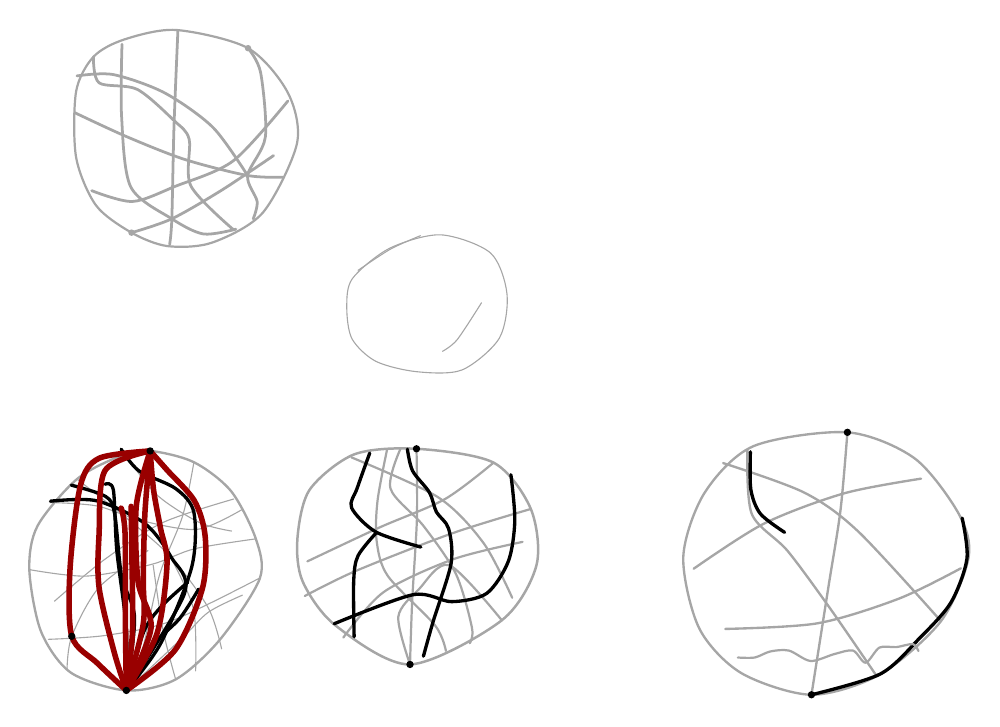
\begin{tikzpicture}[x=.55cm,y=-.55cm,line cap=round,line join=round,g/.style={olive!80!yellow,line width=1.7pt},r/.style={orange!80!brown,line width=1.8pt},w/.style={red!60!black,line width=1.5pt},b/.style={blue!60!black,line width=1.4pt},p/.style={gray!70,thin},k/.style={black,line width=1.2pt},every node/.style={font=\scriptsize}]
% Unlabelled pencil and darker ink arrangements, at their relative positions on the reused sheet.
\draw[p,line width=.8pt] plot[smooth cycle] coordinates {(2.34,7.45) (2.74,6.65) (3.45,6.25) (4.65,6.03) (6.31,6.45) (7.23,7.48) (7.44,8.65) (6.65,10.25) (5.48,10.94) (4.45,11.02) (3.62,10.71) (2.8,10.08) (2.34,8.97)};
\draw[p,line width=1pt] plot[smooth] coordinates {(2.74,6.65) (2.87,7.25) (3.75,7.4) (4.6,8.12) (4.95,8.55) (4.99,9.63) (5.96,10.63)};
\draw[p,line width=1pt] plot[smooth] coordinates {(3.4,6.36) (3.39,8.02) (3.6,9.65) (4.55,10.39) (5.28,10.74) (6.03,10.63)};
\draw[p,line width=1pt] plot[smooth] coordinates {(4.69,6.06) (4.6,8.27) (4.55,10.4) (4.5,10.98)};
\draw[p,line width=1pt] plot[smooth] coordinates {(6.31,6.45) (6.6,7.01) (6.71,8.5) (6.3,9.39) (6.52,9.99) (6.43,10.39)};
\draw[p,line width=1pt] plot[smooth] coordinates {(2.36,7.09) (3.2,7.06) (4.38,7.48) (5.5,8.28) (6.3,9.39)};
\draw[p,line width=1pt] plot[smooth] coordinates {(2.31,7.94) (3.5,8.49) (4.85,9.02) (6.3,9.39) (7.13,9.43)};
\draw[p,line width=1pt] plot[smooth] coordinates {(2.7,9.74) (3.64,9.99) (4.63,9.64) (5.97,9.05) (7.23,7.67)};
\draw[p,line width=1pt] plot[smooth] coordinates {(3.62,10.71) (4.55,10.39) (5.7,9.73) (6.9,8.93)};
\fill[p] (6.31,6.45) circle (.075);
\fill[p] (3.62,10.71) circle (.075);
\draw[p] plot[smooth cycle] coordinates {(8.59,12.43) (8.72,11.77) (9.58,11.07) (10.76,10.76) (11.91,11.18) (12.29,12.13) (12.11,13.15) (11.25,13.88) (10.2,13.92) (9.26,13.68) (8.71,13.16)};
\draw[p] plot[smooth] coordinates {(8.85,11.58) (9.6,11.09) (10.29,10.78)};
\draw[p] plot[smooth] coordinates {(10.8,13.45) (11.14,13.18) (11.7,12.33)};
\draw[p,line width=.85pt] plot[smooth cycle] coordinates {(1.26,18.49) (1.45,17.48) (2.36,16.4) (3.36,15.87) (4.05,15.75) (5.06,16.01) (5.92,16.68) (6.49,17.78) (6.58,18.7) (5.65,20.12) (4.63,21.03) (3.5,21.28) (2.22,20.87) (1.53,19.92)};
\draw[p] plot[smooth] coordinates {(3.38,15.71) (4.19,16.75) (5.18,17.4) (5.93,17.6)};
\draw[p] plot[smooth] coordinates {(5.06,16.01) (4.8,17.25) (4.27,18.6) (3.88,20.3) (3.5,21.28)};
\draw[p] plot[smooth] coordinates {(2.36,16.4) (3.43,17.24) (4.52,18.19) (5.39,19.37) (5.7,20.32)};
\draw[p] plot[smooth] coordinates {(1.73,16.94) (2.82,17.02) (3.85,17.36) (5.14,17.56) (6.16,17.11)};
\draw[p] plot[smooth] coordinates {(1.26,18.49) (2.58,18.64) (4.08,18.37) (5.07,18.01) (6.49,17.78)};
\draw[p] plot[smooth] coordinates {(1.84,19.22) (3.02,18.24) (4.35,17.4) (5.98,16.86)};
\draw[p] plot[smooth] coordinates {(1.7,20.1) (3.02,20.01) (4.53,19.68) (6.57,18.69)};
\draw[p] plot[smooth] coordinates {(2.13,20.8) (2.24,20.03) (2.87,18.9) (4.0,18.05)};
\draw[p] plot[smooth] coordinates {(4.64,21.03) (4.35,19.9) (4.12,18.39)};
\draw[p] plot[smooth] coordinates {(5.1,20.83) (5.05,19.4) (4.52,18.2)};
\draw[p] plot[smooth] coordinates {(3.5,21.28) (4.8,20.06) (5.4,19.47) (6.18,19.08)};
\draw[k] plot[smooth] coordinates {(1.75,16.91) (2.81,16.9) (3.92,17.42) (4.54,18.21) (4.84,19.05) (3.5,21.28)};
\draw[k] plot[smooth] coordinates {(2.23,16.54) (3.02,16.8) (3.23,17.2) (3.39,18.64) (3.69,19.6) (3.5,21.28)};
\draw[k] plot[smooth] coordinates {(3.01,16.52) (3.2,16.65) (3.28,18.05) (3.5,19.85) (3.5,21.28)};
\draw[k] plot[smooth] coordinates {(3.38,15.71) (3.79,16.21) (4.64,16.62) (5.06,17.17) (5.01,18.43) (4.29,20.2) (3.5,21.28)};
\draw[k] plot[smooth] coordinates {(3.5,21.28) (3.9,19.93) (4.31,19.34) (4.92,18.78)};
\draw[k] plot[smooth] coordinates {(3.5,21.28) (4.05,20.3) (4.73,19.62) (5.17,18.94)};
\draw[w,line width=2pt] plot[smooth] coordinates {(4.05,15.75) (2.87,15.92) (2.44,16.55) (2.2,18.47) (2.24,20.03) (2.83,20.65) (3.5,21.28)};
\draw[w,line width=2pt] plot[smooth] coordinates {(4.05,15.75) (3.01,16.2) (2.87,17.68) (2.87,18.9) (3.22,20.4) (3.5,21.28)};
\draw[w,line width=2pt] plot[smooth] coordinates {(4.05,15.75) (3.93,17.17) (3.89,18.7) (3.89,19.75) (3.5,21.28)};
\draw[w,line width=2pt] plot[smooth] coordinates {(4.05,15.75) (4.44,16.19) (5.07,16.9) (5.32,17.72) (5.26,18.91) (4.63,20.34) (3.5,21.28)};
\draw[w,line width=2pt] plot[smooth] coordinates {(4.05,15.75) (4.13,16.66) (4.29,17.54) (4.44,18.35) (4.21,19.96) (3.5,21.28)};
\draw[w,line width=2pt] plot[smooth] coordinates {(4.05,15.75) (3.73,17.02) (3.77,18.76) (4.07,19.84) (3.5,21.28)};
\draw[w,line width=2pt] plot[smooth] coordinates {(3.5,21.28) (3.64,19.95) (3.63,18.29) (3.61,17.03)};
\draw[w,line width=2pt] plot[smooth] coordinates {(3.5,21.28) (3.48,19.85) (3.47,17.65) (3.38,17.07)};
\fill[k] (4.05,15.75) circle (.085);
\fill[k] (3.5,21.28) circle (.085);
\fill[k] (2.24,20.03) circle (.085);
\draw[p,line width=.9pt] plot[smooth cycle] coordinates {(7.45,17.78) (7.73,16.65) (8.76,15.83) (10.2,15.7) (11.98,16.02) (12.84,17.09) (12.97,18.39) (12.17,19.66) (10.05,20.68) (8.33,19.78) (7.57,18.76)};
\draw[p,line width=.8pt] plot[smooth] coordinates {(9.52,15.72) (9.3,16.9) (9.28,17.83) (9.54,18.64) (10.63,19.78) (10.88,20.37)};
\draw[p,line width=.8pt] plot[smooth] coordinates {(9.83,15.7) (9.6,16.62) (10.36,17.48) (11.11,18.59) (11.48,19.83) (11.43,20.19)};
\draw[p,line width=.8pt] plot[smooth] coordinates {(10.2,15.7) (10.21,17.3) (10.1,19.22) (10.05,20.68)};
\draw[p,line width=.8pt] plot[smooth] coordinates {(8.7,15.9) (10.7,16.82) (11.75,17.88) (12.41,19.14)};
\draw[p,line width=.8pt] plot[smooth] coordinates {(7.68,18.3) (9.34,17.52) (10.86,16.86) (11.98,16.02)};
\draw[p,line width=.8pt] plot[smooth] coordinates {(7.62,19.1) (8.8,18.52) (11.03,17.65) (12.84,17.09)};
\draw[p,line width=.8pt] plot[smooth] coordinates {(8.51,20.06) (9.44,19.01) (11.05,18.25) (12.65,17.85)};
\draw[p,line width=.8pt] plot[smooth] coordinates {(10.05,20.68) (9.78,19.58) (10.25,18.95) (10.96,18.39) (12.17,19.66)};
\draw[k] plot[smooth] coordinates {(9.12,15.8) (8.83,16.61) (8.7,17.06) (9.26,17.62) (10.3,17.97)};
\draw[k] plot[smooth] coordinates {(9.99,15.71) (10.11,16.21) (10.5,16.71) (10.66,17.16) (10.94,17.54) (11.0,18.34) (10.59,19.67) (10.36,20.49)};
\draw[k] plot[smooth] coordinates {(12.38,16.3) (12.47,17.36) (12.32,18.3) (11.82,19.04) (11.01,19.23) (10.12,19.07) (8.3,19.74)};
\draw[k] plot[smooth] coordinates {(8.76,20.04) (8.75,18.75) (8.85,18.17) (9.28,17.63)};
\fill[k] (10.2,15.7) circle (.085);
\fill[k] (10.05,20.68) circle (.085);
\draw[p,line width=.85pt] plot[smooth cycle] coordinates {(16.36,18.2) (16.85,16.72) (17.98,15.64) (20.15,15.32) (21.7,15.92) (22.72,17.2) (22.95,18.2) (22.31,19.68) (20.9,20.91) (19.32,21.38) (17.7,20.88) (16.73,19.85)};
\draw[p,line width=.85pt] plot[smooth] coordinates {(17.84,15.73) (17.94,17.2) (18.77,18.06) (19.76,19.4) (20.82,20.94)};
\draw[p,line width=.85pt] plot[smooth] coordinates {(20.15,15.32) (19.99,17.12) (19.71,18.9) (19.32,21.38)};
\draw[p,line width=.85pt] plot[smooth] coordinates {(16.6,18.47) (18.22,17.43) (20.07,16.73) (21.85,16.39)};
\draw[p,line width=.85pt] plot[smooth] coordinates {(17.28,16.03) (19.15,16.71) (20.4,17.61) (22.31,19.68)};
\draw[p,line width=.85pt] plot[smooth] coordinates {(17.33,19.86) (19.46,19.73) (21.34,19.16) (22.77,18.46)};
\draw[k] plot[smooth] coordinates {(17.91,15.77) (17.92,16.64) (18.14,17.2) (18.7,17.63)};
\draw[k] plot[smooth] coordinates {(22.8,17.3) (22.91,18.24) (22.54,19.25) (21.82,20.07) (20.91,20.9) (19.32,21.38)};
\draw[p,line width=.8pt] plot[smooth] coordinates {(17.62,20.52) (18.01,20.52) (18.37,20.38) (18.8,20.36) (19.3,20.6) (19.85,20.44) (20.28,20.36) (20.57,20.64) (20.89,20.29) (21.28,20.28) (21.66,20.21) (21.79,20.37)};
\fill[k] (20.15,15.32) circle (.085);
\fill[k] (19.32,21.38) circle (.085);
\end{tikzpicture}}
\margin{\mspage{146}}

\scanpage{148}
\figure{\begin{tikzpicture}[x=.55cm,y=-.55cm,line cap=round,line join=round,g/.style={olive!80!yellow,line width=1.7pt},r/.style={orange!80!brown,line width=1.8pt},w/.style={red!60!black,line width=1.5pt},b/.style={blue!60!black,line width=1.4pt},p/.style={gray!70,thin},k/.style={black,line width=1.2pt},every node/.style={font=\scriptsize}]
% Large arrangement: pencil construction and overdrawn directed paths.
\draw[p,line width=.9pt] plot[smooth cycle] coordinates {(14.23,2.3) (17.58,2.78) (19.97,3.91) (22.47,7.17) (22.62,9.83) (22.43,11.72) (20.69,15.58) (16.49,18.05) (12.46,18.74) (10.18,18.49) (7.57,17.29) (5.36,14.48) (4.87,11.73) (4.98,9.66) (5.7,7.48) (7.81,4.66) (9.6,3.34) (11.57,2.63)};
\draw[p,line width=.8pt] plot[smooth] coordinates {(14.23,2.3) (11.6,4.38) (9.75,7.88) (9.49,11.44) (10.18,14.83) (11.58,18.17) (12.46,18.74)};
\draw[p,line width=.8pt] plot[smooth] coordinates {(14.23,2.3) (12.01,4.95) (10.25,8.52) (9.5,11.44) (10.49,15.2) (11.94,18.58) (12.46,18.74)};
\draw[p,line width=.8pt] plot[smooth] coordinates {(14.23,2.3) (13.08,4.18) (11.82,7.01) (11.19,11.63) (11.53,15.53) (12.02,18.65) (12.46,18.74)};
\draw[p,line width=.8pt] plot[smooth] coordinates {(14.23,2.3) (13.52,4.95) (12.85,6.65) (11.85,10.3) (12.14,12.29) (12.25,16.57) (12.46,18.74)};
\draw[p,line width=.8pt] plot[smooth] coordinates {(14.23,2.3) (14.15,4.8) (13.54,6.33) (13.27,7.71) (13.59,9.13) (13.89,12.08) (13.79,15.79) (12.46,18.74)};
\draw[p,line width=.8pt] plot[smooth] coordinates {(14.23,2.3) (14.26,5.19) (13.9,7.05) (12.87,11.16) (12.7,15.4) (12.46,18.74)};
\draw[p,line width=.8pt] plot[smooth] coordinates {(14.23,2.3) (14.42,5.38) (14.22,7.49) (13.59,9.13) (13.67,10.95) (13.89,12.08) (14.07,14.64) (12.46,18.74)};
\draw[p,line width=.8pt] plot[smooth] coordinates {(14.23,2.3) (14.47,5.48) (14.72,8.01) (14.24,11.65) (14.47,12.02) (14.28,15.86) (12.46,18.74)};
\draw[p,line width=.8pt] plot[smooth] coordinates {(14.23,2.3) (15.12,3.5) (15.42,5.86) (15.47,7.29) (15.93,8.88) (14.85,12.0) (14.6,15.7) (12.46,18.74)};
\draw[p,line width=.8pt] plot[smooth] coordinates {(14.23,2.3) (15.85,3.35) (16.11,5.32) (16.38,7.2) (16.54,8.64) (15.99,11.53) (15.08,14.27) (14.83,15.65) (16.49,18.05)};
\draw[p,line width=.8pt] plot[smooth] coordinates {(14.23,2.3) (13.66,3.96) (12.85,6.65) (12.79,9.63) (12.82,11.21) (13.28,11.58) (13.11,15.03) (12.46,18.74)};
\draw[p,line width=.7pt] plot[smooth] coordinates {(7.81,4.66) (7.86,7.28) (8.08,10.18) (7.57,12.28) (7.57,17.29)};
\draw[p,line width=.7pt] plot[smooth] coordinates {(7.81,4.66) (8.24,7.49) (8.71,9.19) (8.96,12.32) (9.33,16.09) (10.18,18.49)};
\draw[p,line width=.7pt] plot[smooth] coordinates {(7.81,4.66) (9.75,7.88) (10.95,9.73) (11.85,10.3) (12.82,11.21) (13.89,12.08) (14.58,12.61) (16.81,14.01) (20.69,15.58)};
\draw[p,line width=.7pt] plot[smooth] coordinates {(7.81,4.66) (9.74,5.02) (12.19,6.24) (12.85,6.65) (14.22,7.49) (14.72,8.01) (15.93,8.88) (17.71,10.84) (18.81,12.05) (20.69,15.58)};
\draw[p,line width=.7pt] plot[smooth] coordinates {(11.57,2.63) (12.63,3.76) (13.08,4.18) (13.61,5.12) (13.54,6.33) (13.27,7.71) (13.59,9.13) (14.24,11.65) (14.58,12.61) (15.08,14.27)};
\draw[p,line width=.7pt] plot[smooth] coordinates {(17.58,2.78) (17.01,5.03) (18.98,6.98) (19.39,9.5) (18.81,12.05) (15.36,16.43) (12.46,18.74)};
\draw[p,line width=.7pt] plot[smooth] coordinates {(19.97,3.91) (18.98,6.98) (17.71,10.84) (15.48,15.06) (12.46,18.74)};
\draw[p,line width=.7pt] plot[smooth] coordinates {(5.7,7.48) (7.64,9.54) (8.08,10.18) (9.49,11.44) (11.19,11.63) (12.45,11.74) (12.82,11.21)};
\draw[p,line width=.7pt] plot[smooth] coordinates {(4.87,11.73) (7.57,12.28) (8.96,12.32) (11.19,12.29) (12.14,12.29) (13.89,12.08) (15.88,12.05)};
\draw[p,line width=.7pt] plot[smooth] coordinates {(4.98,9.66) (7.17,8.77) (9.75,7.88) (11.82,7.01) (12.85,6.65) (16.11,5.32) (17.01,5.03) (19.97,3.91)};
\draw[p,line width=.7pt] plot[smooth] coordinates {(4.87,11.73) (7.64,9.54) (10.25,8.52) (11.53,8.14) (13.27,7.71) (14.22,7.49) (15.47,7.29) (16.38,7.2) (18.98,6.98) (22.47,7.17)};
\draw[p,line width=.7pt] plot[smooth] coordinates {(4.9,12.75) (8.08,10.18) (11.2,9.3) (14.72,8.01)};
\draw[p,line width=.7pt] plot[smooth] coordinates {(5.2,13.31) (8.96,11.43) (11.85,10.3) (13.28,9.43) (15.93,8.88) (16.54,8.64) (18.98,6.98)};
\draw[p,line width=.7pt] plot[smooth] coordinates {(5.36,14.48) (9.49,11.44) (12.82,11.21) (15.99,11.53) (17.71,10.84) (20.23,9.54) (22.47,7.17)};
\draw[p,line width=.7pt] plot[smooth] coordinates {(5.79,15.43) (9.33,13.0) (12.14,12.29) (13.89,12.08) (18.81,12.05) (22.43,11.72)};
\draw[p,line width=.7pt] plot[smooth] coordinates {(7.57,17.29) (9.33,16.09) (11.33,13.98) (12.14,12.29) (12.45,11.74) (12.82,11.21)};
\draw[p,line width=.7pt] plot[smooth] coordinates {(7.99,17.65) (9.33,16.78) (10.22,15.72) (11.33,13.98)};
\draw[p,line width=.7pt] plot[smooth] coordinates {(4.87,11.73) (8.08,10.18) (9.49,11.44)};
\draw[p,line width=.7pt] plot[smooth] coordinates {(12.46,18.74) (12.88,15.37) (13.89,12.08) (14.72,8.01)};
\draw[p] (7.69,9.81)--(8.36,9.23);
\draw[p] (7.67,10.01)--(8.44,9.25);
\draw[p] (7.64,10.2)--(8.49,9.2);
\draw[p] (7.61,10.44)--(8.57,9.12);
\draw[p] (8.23,10.5)--(8.08,10.94);
\draw[p] (8.41,10.69)--(8.25,11.2);
\draw[p] (8.59,10.85)--(8.43,11.46);
\draw[p] (8.77,11.01)--(8.6,11.69);
\draw[p] (7.7,12.43)--(7.89,13.0);
\draw[p] (7.98,12.41)--(8.02,13.19);
\draw[p] (8.29,12.4)--(8.04,13.58);
\draw[p] (8.58,12.4)--(8.25,13.86);
\draw[p] (8.75,12.52)--(8.46,14.04);
\draw[p] (13.21,5.45)--(13.65,5.2);
\draw[p] (13.18,5.65)--(13.62,5.42);
\draw[p] (13.12,5.9)--(13.59,5.64);
\draw[p] (13.06,6.13)--(13.55,5.86);
\draw[p] (14.15,10.76)--(14.51,10.44);
\draw[p] (14.12,10.53)--(14.61,10.1);
\draw[p] (14.18,10.26)--(14.7,9.79);
\draw[p] (14.33,9.91)--(14.84,9.53);
\draw[p] (19.2,12.26)--(18.94,13.05);
\draw[p] (19.55,12.25)--(19.24,13.3);
\draw[p] (19.93,12.2)--(19.56,13.67);
\draw[p] (20.31,12.16)--(19.87,13.89);
\draw[p] (20.69,12.12)--(20.27,14.21);
\draw[p] (21.04,12.08)--(20.62,14.4);
\draw[p] (21.42,12.02)--(20.96,14.64);
\draw[w,-stealth,line width=2pt] plot[smooth] coordinates {(4.87,11.73) (6.14,10.64) (7.57,9.7)};
\draw[k,-stealth,line width=1.2pt] plot[smooth] coordinates {(4.87,11.73) (6.14,10.64) (7.57,9.7)};
\draw[w,-stealth,line width=2pt] plot[smooth] coordinates {(4.87,11.73) (6.17,12.1) (7.45,12.31)};
\draw[k,-stealth,line width=1.2pt] plot[smooth] coordinates {(4.87,11.73) (6.17,12.1) (7.45,12.31)};
\draw[w,-stealth,line width=2pt] plot[smooth] coordinates {(5.7,7.48) (6.75,8.46) (7.64,9.54)};
\draw[k,-stealth,line width=1.2pt] plot[smooth] coordinates {(5.7,7.48) (6.75,8.46) (7.64,9.54)};
\draw[w,-stealth,line width=2pt] plot[smooth] coordinates {(7.64,9.54) (8.08,10.18)};
\draw[k,-stealth,line width=1.2pt] plot[smooth] coordinates {(7.64,9.54) (8.08,10.18)};
\draw[w,-stealth,line width=2pt] plot[smooth] coordinates {(7.57,12.28) (8.08,10.18)};
\draw[k,-stealth,line width=1.2pt] plot[smooth] coordinates {(7.57,12.28) (8.08,10.18)};
\draw[w,-stealth,line width=2pt] plot[smooth] coordinates {(7.57,12.28) (8.84,12.33)};
\draw[k,-stealth,line width=1.2pt] plot[smooth] coordinates {(7.57,12.28) (8.84,12.33)};
\draw[w,-stealth,line width=2pt] plot[smooth] coordinates {(8.08,10.18) (9.4,11.39)};
\draw[k,-stealth,line width=1.2pt] plot[smooth] coordinates {(8.08,10.18) (9.4,11.39)};
\draw[w,-stealth,line width=2pt] plot[smooth] coordinates {(8.08,10.18) (8.71,9.19)};
\draw[k,-stealth,line width=1.2pt] plot[smooth] coordinates {(8.08,10.18) (8.71,9.19)};
\draw[w,-stealth,line width=2pt] plot[smooth] coordinates {(8.71,9.19) (9.75,7.88)};
\draw[k,-stealth,line width=1.2pt] plot[smooth] coordinates {(8.71,9.19) (9.75,7.88)};
\draw[w,-stealth,line width=2pt] plot[smooth] coordinates {(7.81,4.66) (8.73,6.63) (9.75,7.88)};
\draw[k,-stealth,line width=1.2pt] plot[smooth] coordinates {(7.81,4.66) (8.73,6.63) (9.75,7.88)};
\draw[w,-stealth,line width=2pt] plot[smooth] coordinates {(9.75,7.88) (10.25,8.52)};
\draw[k,-stealth,line width=1.2pt] plot[smooth] coordinates {(9.75,7.88) (10.25,8.52)};
\draw[w,-stealth,line width=2pt] plot[smooth] coordinates {(10.25,8.52) (11.53,8.14)};
\draw[k,-stealth,line width=1.2pt] plot[smooth] coordinates {(10.25,8.52) (11.53,8.14)};
\draw[w,-stealth,line width=2pt] plot[smooth] coordinates {(10.25,8.52) (10.95,9.73)};
\draw[k,-stealth,line width=1.2pt] plot[smooth] coordinates {(10.25,8.52) (10.95,9.73)};
\draw[w,-stealth,line width=2pt] plot[smooth] coordinates {(10.95,9.73) (11.85,10.3)};
\draw[k,-stealth,line width=1.2pt] plot[smooth] coordinates {(10.95,9.73) (11.85,10.3)};
\draw[w,-stealth,line width=2pt] plot[smooth] coordinates {(9.49,11.44) (11.15,10.65)};
\draw[k,-stealth,line width=1.2pt] plot[smooth] coordinates {(9.49,11.44) (11.15,10.65)};
\draw[w,-stealth,line width=2pt] plot[smooth] coordinates {(11.15,10.65) (11.85,10.3)};
\draw[k,-stealth,line width=1.2pt] plot[smooth] coordinates {(11.15,10.65) (11.85,10.3)};
\draw[w,-stealth,line width=2pt] plot[smooth] coordinates {(9.49,11.44) (11.05,11.67)};
\draw[k,-stealth,line width=1.2pt] plot[smooth] coordinates {(9.49,11.44) (11.05,11.67)};
\draw[w,-stealth,line width=2pt] plot[smooth] coordinates {(8.96,12.32) (9.49,11.44)};
\draw[k,-stealth,line width=1.2pt] plot[smooth] coordinates {(8.96,12.32) (9.49,11.44)};
\draw[w,-stealth,line width=2pt] plot[smooth] coordinates {(11.19,12.29) (12.14,12.29)};
\draw[k,-stealth,line width=1.2pt] plot[smooth] coordinates {(11.19,12.29) (12.14,12.29)};
\draw[w,-stealth,line width=2pt] plot[smooth] coordinates {(11.85,10.3) (12.72,11.15)};
\draw[k,-stealth,line width=1.2pt] plot[smooth] coordinates {(11.85,10.3) (12.72,11.15)};
\draw[w,-stealth,line width=2pt] plot[smooth] coordinates {(12.14,12.29) (12.45,11.74)};
\draw[k,-stealth,line width=1.2pt] plot[smooth] coordinates {(12.14,12.29) (12.45,11.74)};
\draw[w,-stealth,line width=2pt] plot[smooth] coordinates {(12.45,11.74) (12.82,11.21)};
\draw[k,-stealth,line width=1.2pt] plot[smooth] coordinates {(12.45,11.74) (12.82,11.21)};
\draw[w,-stealth,line width=2pt] plot[smooth] coordinates {(12.82,11.21) (13.28,11.58)};
\draw[k,-stealth,line width=1.2pt] plot[smooth] coordinates {(12.82,11.21) (13.28,11.58)};
\draw[w,-stealth,line width=2pt] plot[smooth] coordinates {(13.28,11.58) (13.89,12.08)};
\draw[k,-stealth,line width=1.2pt] plot[smooth] coordinates {(13.28,11.58) (13.89,12.08)};
\draw[w,-stealth,line width=2pt] plot[smooth] coordinates {(13.89,12.08) (14.47,12.02)};
\draw[k,-stealth,line width=1.2pt] plot[smooth] coordinates {(13.89,12.08) (14.47,12.02)};
\draw[w,-stealth,line width=2pt] plot[smooth] coordinates {(14.47,12.02) (15.99,11.53)};
\draw[k,-stealth,line width=1.2pt] plot[smooth] coordinates {(14.47,12.02) (15.99,11.53)};
\draw[w,-stealth,line width=2pt] plot[smooth] coordinates {(15.99,11.53) (17.71,10.84)};
\draw[k,-stealth,line width=1.2pt] plot[smooth] coordinates {(15.99,11.53) (17.71,10.84)};
\draw[w,-stealth,line width=2pt] plot[smooth] coordinates {(17.71,10.84) (18.81,12.05)};
\draw[k,-stealth,line width=1.2pt] plot[smooth] coordinates {(17.71,10.84) (18.81,12.05)};
\draw[w,-stealth,line width=2pt] plot[smooth] coordinates {(18.81,12.05) (22.43,11.72)};
\draw[k,-stealth,line width=1.2pt] plot[smooth] coordinates {(18.81,12.05) (22.43,11.72)};
\draw[w,-stealth,line width=2pt] plot[smooth] coordinates {(18.81,12.05) (19.83,14.29) (20.69,15.58)};
\draw[k,-stealth,line width=1.2pt] plot[smooth] coordinates {(18.81,12.05) (19.83,14.29) (20.69,15.58)};
\draw[w,-stealth,line width=2pt] plot[smooth] coordinates {(7.57,17.29) (7.55,14.8) (7.57,12.28)};
\draw[k,-stealth,line width=1.2pt] plot[smooth] coordinates {(7.57,17.29) (7.55,14.8) (7.57,12.28)};
\draw[w,-stealth,line width=2pt] plot[smooth] coordinates {(7.57,17.29) (9.33,16.09)};
\draw[k,-stealth,line width=1.2pt] plot[smooth] coordinates {(7.57,17.29) (9.33,16.09)};
\draw[w,-stealth,line width=2pt] plot[smooth] coordinates {(10.18,18.49) (9.33,16.09)};
\draw[k,-stealth,line width=1.2pt] plot[smooth] coordinates {(10.18,18.49) (9.33,16.09)};
\draw[w,-stealth,line width=2pt] plot[smooth] coordinates {(8.96,15.41) (8.87,13.87) (8.96,12.32)};
\draw[k,-stealth,line width=1.2pt] plot[smooth] coordinates {(8.96,15.41) (8.87,13.87) (8.96,12.32)};
\draw[w,-stealth,line width=2pt] plot[smooth] coordinates {(11.33,13.98) (12.14,12.29)};
\draw[k,-stealth,line width=1.2pt] plot[smooth] coordinates {(11.33,13.98) (12.14,12.29)};
\draw[w,-stealth,line width=2pt] plot[smooth] coordinates {(12.19,6.24) (12.85,6.65)};
\draw[k,-stealth,line width=1.2pt] plot[smooth] coordinates {(12.19,6.24) (12.85,6.65)};
\draw[w,-stealth,line width=2pt] plot[smooth] coordinates {(11.82,7.01) (12.85,6.65)};
\draw[k,-stealth,line width=1.2pt] plot[smooth] coordinates {(11.82,7.01) (12.85,6.65)};
\draw[w,-stealth,line width=2pt] plot[smooth] coordinates {(12.85,6.65) (13.54,6.33)};
\draw[k,-stealth,line width=1.2pt] plot[smooth] coordinates {(12.85,6.65) (13.54,6.33)};
\draw[w,-stealth,line width=2pt] plot[smooth] coordinates {(13.54,6.33) (13.27,7.71)};
\draw[k,-stealth,line width=1.2pt] plot[smooth] coordinates {(13.54,6.33) (13.27,7.71)};
\draw[w,-stealth,line width=2pt] plot[smooth] coordinates {(13.27,7.71) (14.22,7.49)};
\draw[k,-stealth,line width=1.2pt] plot[smooth] coordinates {(13.27,7.71) (14.22,7.49)};
\draw[w,-stealth,line width=2pt] plot[smooth] coordinates {(14.22,7.49) (14.72,8.01)};
\draw[k,-stealth,line width=1.2pt] plot[smooth] coordinates {(14.22,7.49) (14.72,8.01)};
\draw[w,-stealth,line width=2pt] plot[smooth] coordinates {(13.27,7.71) (13.59,9.13)};
\draw[k,-stealth,line width=1.2pt] plot[smooth] coordinates {(13.27,7.71) (13.59,9.13)};
\draw[w,-stealth,line width=2pt] plot[smooth] coordinates {(13.59,9.13) (14.72,8.01)};
\draw[k,-stealth,line width=1.2pt] plot[smooth] coordinates {(13.59,9.13) (14.72,8.01)};
\draw[w,-stealth,line width=2pt] plot[smooth] coordinates {(13.59,9.13) (13.72,9.97)};
\draw[k,-stealth,line width=1.2pt] plot[smooth] coordinates {(13.59,9.13) (13.72,9.97)};
\draw[w,-stealth,line width=2pt] plot[smooth] coordinates {(13.72,9.97) (14.24,11.65)};
\draw[k,-stealth,line width=1.2pt] plot[smooth] coordinates {(13.72,9.97) (14.24,11.65)};
\draw[w,-stealth,line width=2pt] plot[smooth] coordinates {(14.24,11.65) (14.47,12.02)};
\draw[k,-stealth,line width=1.2pt] plot[smooth] coordinates {(14.24,11.65) (14.47,12.02)};
\draw[w,-stealth,line width=2pt] plot[smooth] coordinates {(14.72,8.01) (15.47,7.29)};
\draw[k,-stealth,line width=1.2pt] plot[smooth] coordinates {(14.72,8.01) (15.47,7.29)};
\draw[w,-stealth,line width=2pt] plot[smooth] coordinates {(14.72,8.01) (15.93,8.88)};
\draw[k,-stealth,line width=1.2pt] plot[smooth] coordinates {(14.72,8.01) (15.93,8.88)};
\draw[w,-stealth,line width=2pt] plot[smooth] coordinates {(15.47,7.29) (16.38,7.2)};
\draw[k,-stealth,line width=1.2pt] plot[smooth] coordinates {(15.47,7.29) (16.38,7.2)};
\draw[w,-stealth,line width=2pt] plot[smooth] coordinates {(16.38,7.2) (18.98,6.98)};
\draw[k,-stealth,line width=1.2pt] plot[smooth] coordinates {(16.38,7.2) (18.98,6.98)};
\draw[w,-stealth,line width=2pt] plot[smooth] coordinates {(18.98,6.98) (22.47,7.17)};
\draw[k,-stealth,line width=1.2pt] plot[smooth] coordinates {(18.98,6.98) (22.47,7.17)};
\draw[w,-stealth,line width=2pt] plot[smooth] coordinates {(18.98,6.98) (19.65,5.6) (19.97,3.91)};
\draw[k,-stealth,line width=1.2pt] plot[smooth] coordinates {(18.98,6.98) (19.65,5.6) (19.97,3.91)};
\draw[w,-stealth,line width=2pt] plot[smooth] coordinates {(15.93,8.88) (16.54,8.64)};
\draw[k,-stealth,line width=1.2pt] plot[smooth] coordinates {(15.93,8.88) (16.54,8.64)};
\draw[w,-stealth,line width=2pt] plot[smooth] coordinates {(16.54,8.64) (18.05,7.98) (18.98,6.98)};
\draw[k,-stealth,line width=1.2pt] plot[smooth] coordinates {(16.54,8.64) (18.05,7.98) (18.98,6.98)};
\draw[w,-stealth,line width=2pt] plot[smooth] coordinates {(15.93,8.88) (16.45,9.48)};
\draw[k,-stealth,line width=1.2pt] plot[smooth] coordinates {(15.93,8.88) (16.45,9.48)};
\draw[w,-stealth,line width=2pt] plot[smooth] coordinates {(16.45,9.48) (17.71,10.84)};
\draw[k,-stealth,line width=1.2pt] plot[smooth] coordinates {(16.45,9.48) (17.71,10.84)};
\draw[w,-stealth,line width=2pt] plot[smooth] coordinates {(15.47,7.29) (16.35,6.19)};
\draw[k,-stealth,line width=1.2pt] plot[smooth] coordinates {(15.47,7.29) (16.35,6.19)};
\draw[w,-stealth,line width=2pt] plot[smooth] coordinates {(16.35,6.19) (17.01,5.03)};
\draw[k,-stealth,line width=1.2pt] plot[smooth] coordinates {(16.35,6.19) (17.01,5.03)};
\draw[w,-stealth,line width=2pt] plot[smooth] coordinates {(16.11,5.32) (17.01,5.03)};
\draw[k,-stealth,line width=1.2pt] plot[smooth] coordinates {(16.11,5.32) (17.01,5.03)};
\draw[w,-stealth,line width=2pt] plot[smooth] coordinates {(17.01,5.03) (19.88,4.07)};
\draw[k,-stealth,line width=1.2pt] plot[smooth] coordinates {(17.01,5.03) (19.88,4.07)};
\draw[w,-stealth,line width=2pt] plot[smooth] coordinates {(17.01,5.03) (17.58,2.78)};
\draw[k,-stealth,line width=1.2pt] plot[smooth] coordinates {(17.01,5.03) (17.58,2.78)};
\draw[k,thin,-stealth] plot[smooth] coordinates {(14.47,12.02) (15.88,12.05)};
\draw[k,thin,-stealth] plot[smooth] coordinates {(14.58,12.61) (15.53,13.14)};
\draw[k,thin,-stealth] plot[smooth] coordinates {(14.59,13.17) (15.08,14.27)};
\draw[k,thin,-stealth] plot[smooth] coordinates {(12.85,6.65) (13.08,4.18)};
\draw[k,thin,-stealth] plot[smooth] coordinates {(13.85,6.2) (16.11,5.32)};
\fill[k] (14.23,2.3) circle (.18);
\fill[k] (12.46,18.74) circle (.18);
\fill[k] (7.81,4.66) circle (.065);
\fill[k] (4.87,11.73) circle (.065);
\fill[k] (7.57,17.29) circle (.065);
\fill[k] (7.57,12.28) circle (.065);
\fill[k] (8.08,10.18) circle (.065);
\fill[k] (8.96,12.32) circle (.065);
\fill[k] (9.33,16.09) circle (.065);
\fill[k] (9.49,11.44) circle (.065);
\fill[k] (9.75,7.88) circle (.065);
\fill[k] (10.25,8.52) circle (.065);
\fill[k] (11.53,8.14) circle (.065);
\fill[k] (11.85,10.3) circle (.065);
\fill[k] (12.14,12.29) circle (.065);
\fill[k] (12.45,11.74) circle (.065);
\fill[k] (12.82,11.21) circle (.065);
\fill[k] (13.28,11.58) circle (.065);
\fill[k] (13.89,12.08) circle (.065);
\fill[k] (14.24,11.65) circle (.065);
\fill[k] (14.47,12.02) circle (.065);
\fill[k] (15.99,11.53) circle (.065);
\fill[k] (15.88,12.05) circle (.065);
\fill[k] (17.71,10.84) circle (.065);
\fill[k] (18.81,12.05) circle (.065);
\fill[k] (20.69,15.58) circle (.065);
\fill[k] (22.47,7.17) circle (.065);
\fill[k] (19.97,3.91) circle (.065);
\fill[k] (18.98,6.98) circle (.065);
\fill[k] (17.01,5.03) circle (.065);
\fill[k] (16.11,5.32) circle (.065);
\fill[k] (16.35,6.19) circle (.065);
\fill[k] (16.38,7.2) circle (.065);
\fill[k] (16.54,8.64) circle (.065);
\fill[k] (15.93,8.88) circle (.065);
\fill[k] (14.72,8.01) circle (.065);
\fill[k] (14.22,7.49) circle (.065);
\fill[k] (13.59,9.13) circle (.065);
\fill[k] (13.54,6.33) circle (.065);
\fill[k] (12.85,6.65) circle (.065);
\fill[k] (12.19,6.24) circle (.065);
\fill[k] (11.82,7.01) circle (.065);
\fill[k] (13.08,4.18) circle (.065);
\node at (7.87,4.36) {$1,2,3,4$};
\node at (7.71,5.46) {$1$};
\node at (7.66,6.36) {$1$};
\node at (7.49,6.98) {$2$};
\node at (7.91,7.34) {$3$};
\node at (8.25,7.54) {$4$};
\node at (6.18,6.34) {$1$};
\node at (4.59,11.72) {$1$};
\node at (7.75,9.4) {$2$};
\node at (8.32,10.24) {$3$};
\node at (8.83,9.43) {$4$};
\node at (9.94,7.79) {$5$};
\node at (10.43,8.56) {$6$};
\node at (11.73,8.3) {$7$};
\node at (11.35,9.04) {$6$};
\node at (11.36,9.73) {$7$};
\node at (11.29,10.81) {$7$};
\node at (11.47,11.76) {$7$};
\node at (11.65,14.05) {$\unsure{7}$};
\node at (12.34,12.52) {$8$};
\node at (12.58,11.89) {$\unsure{8|9}$};
\node at (12.99,11.19) {$10$};
\node at (13.43,11.45) {$11$};
\node at (13.93,12.43) {$12$};
\node at (13.88,12.6) {$\unsure{13,14}$};
\node at (14.63,12.17) {$15$};
\node at (14.89,12.63) {$16$};
\node at (14.39,11.22) {$14$};
\node at (14.25,10.05) {$13$};
\node at (13.77,8.75) {$12$};
\node at (13.55,7.84) {$11$};
\node at (13.75,7.01) {$10$};
\node at (13.74,5.93) {$9$};
\node at (13.94,5.95) {$10$};
\node at (14.15,5.96) {$11$};
\node at (14.53,5.85) {$12$};
\node at (14.95,5.64) {$13$};
\node at (15.3,5.3) {$14$};
\node at (12.91,5.75) {$8$};
\node at (12.21,5.98) {$7$};
\node at (11.94,6.6) {$7$};
\node at (12.85,7.02) {$8$};
\node at (13.44,6.25) {$\unsure{9|3}$};
\node at (12.97,4.42) {$7$};
\node at (10.1,6.67) {$5$};
\node at (10.87,6.8) {$6$};
\node at (8.87,10.48) {$4$};
\node at (7.47,10.89) {$\unsure{2}$};
\node at (7.35,12.48) {$2$};
\node at (9.17,12.61) {$3$};
\node at (9.46,11.87) {$4$};
\node at (7.43,17.68) {$1$};
\node at (9.69,16.16) {$2$};
\node at (8.21,14.02) {$2$};
\node at (9.76,14.19) {$3$};
\node at (10.2,13.66) {$5$};
\node at (14.96,10.91) {$15$};
\node at (15.25,10.93) {$16$};
\node at (16.21,11.67) {$17$};
\node at (16.18,12.45) {$17$};
\node at (15.82,13.34) {$17$};
\node at (15.36,14.58) {$17$};
\node at (17.93,10.66) {$18$};
\node at (16.66,9.47) {$17$};
\node at (16.88,8.68) {$17$};
\node at (16.91,7.2) {$17$};
\node at (16.7,6.26) {$17$};
\node at (16.14,4.93) {$17$};
\node at (17.76,5.83) {$18$};
\node at (18.4,9.17) {$18$};
\node at (19.43,8.98) {$19$};
\node at (19.32,3.34) {$17=1$};
\node at (17.02,4.47) {$18,19$};
\node at (19.13,6.76) {$18,19$};
\node at (15.77,7.61) {$\begin{gathered}14\\15,16\end{gathered}$};
\node at (16.01,8.51) {$\unsure{14,15,16}$};
\node at (12.18,10.5) {$\unsure{8,9}$};
\draw[k,thin] (7.87,4.36) ellipse (0.7 and 0.47);
\draw[k,thin] (17.02,4.47) ellipse (0.48 and 0.49);
\draw[k,thin] (19.13,6.76) ellipse (0.58 and 0.5);
\draw[k,thin] (15.77,7.61) ellipse (0.4 and 0.37);
\draw[k,thin] (16.01,8.51) ellipse (0.33 and 0.33);
\draw[k,thin] (12.18,10.5) ellipse (0.37 and 0.31);
\draw[k,thin] (13.88,12.6) ellipse (0.3 and 0.4);
\draw[k,dashed] plot[smooth] coordinates {(7.66,4.9) (7.7,7.25) (7.65,9.4)};
\draw[k,dashed] plot[smooth] coordinates {(9.6,16.4) (10.18,17.25) (11.59,18.35)};
% Upper-right local three-line crossing with two hatched sectors.
\draw[p,line width=.8pt] plot[smooth] coordinates {(24.9,6.35) (26.22,6.04) (28.13,5.54)};
\draw[p,line width=.8pt] plot[smooth] coordinates {(25.3,4.16) (26.22,6.04) (27.2,7.5)};
\draw[p,line width=.8pt] plot[smooth] coordinates {(25.29,7.52) (26.22,6.04) (27.31,4.23)};
\fill[k] (26.22,6.04) circle (.18);
\draw[p,->] plot[smooth] coordinates {(26.8,5.72) (26.1,5.4) (25.68,5.71)};
\draw[p] (24.97,6.36)--(25.15,6.12);
\draw[p] (25.15,6.33)--(25.33,6.09);
\draw[p] (25.33,6.29)--(25.509999999999998,6.05);
\draw[p] (25.51,6.25)--(25.69,6.01);
\draw[p] (25.69,6.2)--(25.87,5.96);
\draw[p] (26.55,5.96)--(26.73,5.72);
\draw[p] (26.72,5.92)--(26.9,5.68);
\draw[p] (26.88,5.88)--(27.06,5.64);
\draw[p] (27.06,5.84)--(27.24,5.6);
\draw[p] (27.24,5.8)--(27.419999999999998,5.56);
% Lower-right unlabelled arrow network over a pencil oval.
\draw[p] plot[smooth cycle] coordinates {(21.31,16.45) (21.62,15.32) (22.78,14.27) (24.03,14.17) (25.6,14.66) (26.39,15.8) (26.42,17.1) (25.69,18.51) (24.53,19.15) (23.03,19.23) (22.01,18.78) (21.38,17.71)};
\draw[k,->,line width=.8pt] plot[smooth] coordinates {(22.02,19.0) (22.23,17.05)};
\draw[k,->,line width=.8pt] plot[smooth] coordinates {(22.02,19.0) (23.22,18.48)};
\draw[k,->,line width=.8pt] plot[smooth] coordinates {(23.42,19.24) (23.22,18.57)};
\draw[k,->,line width=.8pt] plot[smooth] coordinates {(22.24,17.05) (23.15,17.22)};
\draw[k,->,line width=.8pt] plot[smooth] coordinates {(23.18,18.18) (23.23,17.39)};
\draw[k,->,line width=.8pt] plot[smooth] coordinates {(21.37,16.48) (22.15,16.94)};
\draw[k,->,line width=.8pt] plot[smooth] coordinates {(21.36,16.29) (22.38,15.44)};
\draw[k,->,line width=.8pt] plot[smooth] coordinates {(22.2,16.92) (22.54,15.55)};
\draw[k,->,line width=.8pt] plot[smooth] coordinates {(22.41,16.9) (22.84,16.06)};
\draw[k,->,line width=.8pt] plot[smooth] coordinates {(22.58,15.5) (22.91,15.87)};
\draw[k,->,line width=.8pt] plot[smooth] coordinates {(22.91,15.98) (23.38,16.56)};
\draw[k,->,line width=.8pt] plot[smooth] coordinates {(23.25,17.12) (23.47,16.66)};
\draw[k,->,line width=.8pt] plot[smooth] coordinates {(23.55,16.65) (24.13,16.73)};
\draw[k,->,line width=.8pt] plot[smooth] coordinates {(23.5,16.52) (24.19,16.1)};
\draw[k,->,line width=.8pt] plot[smooth] coordinates {(23.54,16.53) (24.61,16.03)};
\draw[k,->,line width=.8pt] plot[smooth] coordinates {(23.22,15.01) (23.69,15.54)};
\draw[k,->,line width=.8pt] plot[smooth] coordinates {(23.7,15.56) (24.15,15.95)};
\draw[k,->,line width=.8pt] plot[smooth] coordinates {(22.88,15.49) (23.31,14.91)};
\draw[k,->,line width=.8pt] plot[smooth] coordinates {(22.25,14.85) (22.39,15.38)};
\draw[k,->,line width=.8pt] plot[smooth] coordinates {(23.02,14.34) (23.42,14.79)};
\draw[k,->,line width=.8pt] plot[smooth] coordinates {(23.44,14.82) (24.04,14.69)};
\draw[k,->,line width=.8pt] plot[smooth] coordinates {(23.51,15.07) (24.18,14.99)};
\draw[k,->,line width=.8pt] plot[smooth] coordinates {(24.01,17.95) (24.58,17.4)};
\draw[k,->,line width=.8pt] plot[smooth] coordinates {(24.57,17.13) (24.76,16.65)};
\draw[k,->,line width=.8pt] plot[smooth] coordinates {(24.87,16.32) (25.18,16.56)};
\draw[k,->,line width=.8pt] plot[smooth] coordinates {(25.13,16.74) (25.53,17.05)};
\draw[k,->,line width=.8pt] plot[smooth] coordinates {(25.53,17.05) (26.04,17.01)};
\draw[k,->,line width=.8pt] plot[smooth] coordinates {(26.11,17.02) (26.63,16.82)};
\draw[k,->,line width=.8pt] plot[smooth] coordinates {(26.13,17.12) (27.0,17.27)};
\draw[k,->,line width=.8pt] plot[smooth] coordinates {(26.98,17.27) (28.1,17.13)};
\draw[k,->,line width=.8pt] plot[smooth] coordinates {(27.39,17.53) (27.95,18.08)};
\draw[k,->,line width=.8pt] plot[smooth] coordinates {(27.07,17.28) (27.24,17.63)};
\draw[k,->,line width=.8pt] plot[smooth] coordinates {(24.49,14.39) (24.79,14.57)};
\draw[k,->,line width=.8pt] plot[smooth] coordinates {(24.53,14.66) (24.99,14.67)};
\draw[k,->,line width=.8pt] plot[smooth] coordinates {(25.02,14.67) (25.45,14.65)};
\draw[k,->,line width=.8pt] plot[smooth] coordinates {(25.35,14.8) (25.27,15.13)};
\draw[k,->,line width=.8pt] plot[smooth] coordinates {(25.26,15.21) (25.26,15.59)};
\draw[k,->,line width=.8pt] plot[smooth] coordinates {(25.27,15.68) (25.43,15.99)};
\draw[k,->,line width=.8pt] plot[smooth] coordinates {(25.48,16.1) (25.67,16.4)};
\draw[k,->,line width=.8pt] plot[smooth] coordinates {(25.43,15.65) (25.87,15.39)};
\draw[k,->,line width=.8pt] plot[smooth] coordinates {(25.7,16.36) (26.45,16.13)};
\draw[k,->,line width=.8pt] plot[smooth] coordinates {(25.61,15.94) (26.09,15.69)};
\draw[k,->,line width=.8pt] plot[smooth] coordinates {(26.01,15.4) (26.2,15.64)};
\draw[k,->,line width=.8pt] plot[smooth] coordinates {(26.19,15.68) (26.46,15.95)};
\draw[k,->,line width=.8pt] plot[smooth] coordinates {(26.5,16.01) (26.89,15.87)};
\draw[k,->,line width=.8pt] plot[smooth] coordinates {(26.49,16.17) (26.88,16.42)};
\draw[k,->,line width=.8pt] plot[smooth] coordinates {(26.96,16.45) (27.29,16.8)};
\draw[k,->,line width=.8pt] plot[smooth] coordinates {(26.58,15.53) (26.93,15.47)};
\draw[k,->,line width=.8pt] plot[smooth] coordinates {(26.96,15.48) (27.62,15.55)};
\draw[k,->,line width=.8pt] plot[smooth] coordinates {(26.53,15.3) (26.69,14.78)};
\draw[k,->,line width=.8pt] plot[smooth] coordinates {(26.83,14.57) (27.04,14.23)};
\draw[k,->,line width=.8pt] plot[smooth] coordinates {(26.42,14.23) (26.82,14.23)};
\draw[k,->,line width=.8pt] plot[smooth] coordinates {(27.05,14.21) (27.58,14.22)};
\draw[k,->,line width=.8pt] plot[smooth] coordinates {(27.62,15.43) (27.66,14.4)};
\draw[k,->,line width=.8pt] plot[smooth] coordinates {(27.05,15.83) (27.62,15.62)};
\draw[k,->,line width=.8pt] plot[smooth] coordinates {(27.1,14.16) (27.2,13.65)};
\draw[k,->,line width=.8pt] plot[smooth] coordinates {(24.18,17.34) (24.58,17.33)};
\draw[k,line width=1.4pt] (26.63,17.2)--(27.0,16.95)--(27.4,17.34)--(26.96,17.03)--(26.65,17.49)--(27.13,17.14)--(27.43,17.38)--(27.42,17.12);
\draw[k,line width=1.4pt] (23.7,14.84)--(23.96,14.72)--(23.8,14.85)--(24.1,14.71);
\end{tikzpicture}}
\margin{\mspage{147}}

\scanpage{149}
\figure{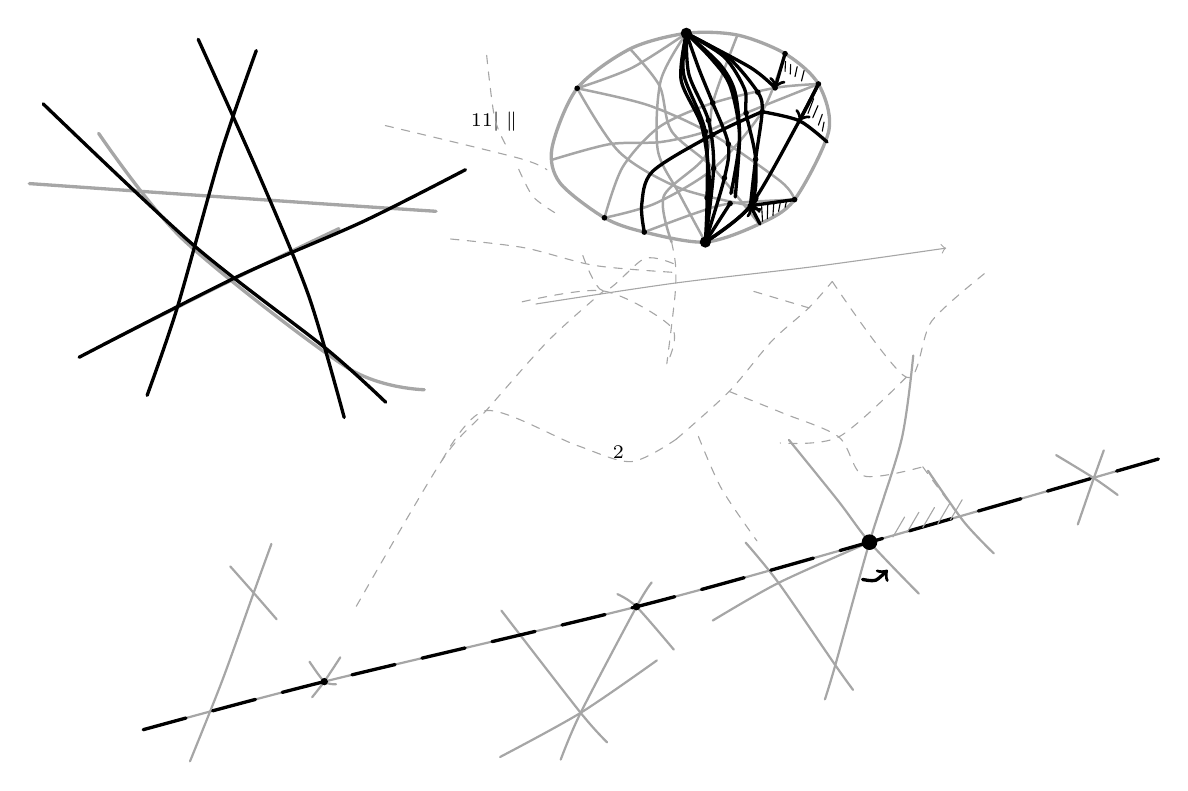
\begin{tikzpicture}[x=.55cm,y=-.55cm,line cap=round,line join=round,g/.style={olive!80!yellow,line width=1.7pt},r/.style={orange!80!brown,line width=1.8pt},w/.style={red!60!black,line width=1.5pt},b/.style={blue!60!black,line width=1.4pt},p/.style={gray!70,thin},k/.style={black,line width=1.2pt},every node/.style={font=\scriptsize}]
% Upper-left crossing lines.
\draw[p,line width=1.2pt] plot[smooth] coordinates {(1.95,5.64) (5.4,5.88) (8.91,6.12) (11.34,6.28)};
\draw[p,line width=1.2pt] plot[smooth] coordinates {(3.65,9.36) (6.7,7.83) (9.1,6.68)};
\draw[p,line width=1.2pt] plot[smooth] coordinates {(3.55,4.48) (5.51,6.94) (9.31,9.9) (11.07,10.4)};
\draw[k] plot[smooth] coordinates {(2.27,3.8) (5.74,7.06) (8.8,9.45) (10.18,10.69)};
\draw[k] plot[smooth] coordinates {(5.85,2.31) (7.24,5.41) (8.4,8.23) (9.22,11.04)};
\draw[k] plot[smooth] coordinates {(7.19,2.57) (6.37,4.95) (5.37,8.49) (4.67,10.53)};
\draw[k] plot[smooth] coordinates {(3.1,9.65) (6.73,7.8) (9.67,6.51) (12.02,5.32)};
% Upper central oval arrangement, marked points and hatched sectors.
\draw[p,line width=1.2pt] plot[smooth cycle] coordinates {(17.12,2.17) (18.3,2.21) (19.4,2.64) (20.17,3.34) (20.41,4.42) (19.62,6.01) (18.81,6.57) (17.56,6.99) (16.15,6.76) (15.23,6.43) (14.2,5.62) (14.02,4.81) (14.6,3.44) (15.82,2.53)};
\draw[p,line width=.9pt] plot[smooth] coordinates {(17.12,2.17) (16.53,3.26) (16.46,4.86) (16.96,5.88) (17.56,6.99)};
\draw[p,line width=.9pt] plot[smooth] coordinates {(18.3,2.21) (17.73,3.78) (17.57,4.99) (16.6,5.93) (16.78,6.99)};
\draw[p,line width=.9pt] plot[smooth] coordinates {(19.4,2.64) (18.87,3.98) (17.75,5.29) (16.4,6.1) (15.23,6.43)};
\draw[p,line width=.9pt] plot[smooth] coordinates {(15.82,2.53) (16.5,3.38) (16.78,4.43) (17.75,5.29) (18.8,6.57)};
\draw[p,line width=.9pt] plot[smooth] coordinates {(14.6,3.44) (15.57,4.91) (16.98,5.75) (18.6,6.15)};
\draw[p,line width=.9pt] plot[smooth] coordinates {(14.6,3.44) (15.86,2.97) (17.12,2.17)};
\draw[p,line width=.9pt] plot[smooth] coordinates {(14.6,3.44) (16.24,3.83) (17.73,4.51) (19.3,5.59) (19.62,6.01)};
\draw[p,line width=.9pt] plot[smooth] coordinates {(14.02,5.09) (15.35,4.73) (16.53,4.68) (17.57,4.44) (18.5,4.01) (20.17,3.34)};
\draw[p,line width=.9pt] plot[smooth] coordinates {(15.23,6.43) (15.65,5.26) (16.5,4.33) (17.73,3.78) (19.17,3.43) (20.17,3.34)};
\draw[p,line width=.9pt] plot[smooth] coordinates {(16.15,6.76) (17.34,6.32) (18.13,6.1) (19.62,6.01)};
\draw[k] plot[smooth] coordinates {(17.12,2.17) (17.0,3.25) (17.48,4.33) (17.66,5.7) (17.56,6.99)};
\draw[k] plot[smooth] coordinates {(17.12,2.17) (17.06,3.12) (17.56,4.44) (17.6,5.97) (17.56,6.99)};
\draw[k] plot[smooth] coordinates {(17.12,2.17) (17.18,3.12) (17.63,4.18) (17.75,5.29) (17.56,6.99)};
\draw[k] plot[smooth] coordinates {(17.12,2.17) (17.41,2.99) (17.73,3.78) (18.09,4.73) (18.0,5.51) (17.56,6.99)};
\draw[k] plot[smooth] coordinates {(17.12,2.17) (17.89,2.88) (18.24,3.51) (18.35,4.55) (18.25,5.95)};
\draw[k] plot[smooth] coordinates {(17.12,2.17) (18.0,2.72) (18.47,3.47) (18.5,4.01) (18.72,5.08) (18.6,6.15) (17.56,6.99)};
\draw[k] plot[smooth] coordinates {(17.12,2.17) (18.08,2.72) (18.77,3.53) (18.87,3.98) (18.72,5.08) (18.6,6.15)};
\draw[k] plot[smooth] coordinates {(17.12,2.17) (18.6,2.96) (19.17,3.43)};
\draw[k] plot[smooth] coordinates {(16.15,6.76) (16.09,6.13) (16.34,5.36) (17.73,4.51) (18.87,3.98)};
\draw[k] plot[smooth] coordinates {(18.87,3.98) (19.73,4.19) (20.37,4.68)};
\draw[k] plot[smooth] coordinates {(17.56,6.99) (18.13,6.1)};
\draw[k] plot[smooth] coordinates {(17.56,6.99) (18.6,6.15) (19.73,4.19) (20.17,3.34)};
\draw[k] plot[smooth] coordinates {(17.12,2.17) (17.7,2.76) (18.13,3.38) (18.35,4.55) (18.15,5.87)};
\fill[k] (17.12,2.17) circle (.13);
\fill[k] (17.56,6.99) circle (.13);
\fill[k] (14.6,3.44) circle (.065);
\fill[k] (15.23,6.43) circle (.065);
\fill[k] (16.15,6.76) circle (.065);
\fill[k] (19.62,6.01) circle (.065);
\fill[k] (18.6,6.15) circle (.065);
\fill[k] (18.13,6.1) circle (.065);
\fill[k] (17.6,5.97) circle (.065);
\fill[k] (17.66,5.7) circle (.065);
\fill[k] (17.75,5.29) circle (.065);
\fill[k] (18.0,5.51) circle (.065);
\fill[k] (18.72,5.08) circle (.065);
\fill[k] (18.09,4.73) circle (.065);
\fill[k] (17.73,4.51) circle (.065);
\fill[k] (17.56,4.44) circle (.065);
\fill[k] (17.63,4.18) circle (.065);
\fill[k] (17.73,3.78) circle (.065);
\fill[k] (18.5,4.01) circle (.065);
\fill[k] (18.87,3.98) circle (.065);
\fill[k] (18.77,3.53) circle (.065);
\fill[k] (19.17,3.43) circle (.065);
\fill[k] (19.73,4.19) circle (.065);
\fill[k] (20.17,3.34) circle (.065);
\fill[k] (19.4,2.64) circle (.065);
\draw[k,->] plot[smooth] coordinates {(20.17,3.34) (19.73,4.19)};
\draw[k,->] plot[smooth] coordinates {(19.4,2.64) (19.17,3.43)};
\draw[k,->] plot[smooth] coordinates {(19.62,6.01) (18.6,6.15)};
\draw[k,->] plot[smooth] coordinates {(18.82,6.57) (18.6,6.15)};
\draw[k,thin] plot[smooth] coordinates {(19.41,2.82) (19.4,3.05)};
\draw[k,thin] plot[smooth] coordinates {(19.53,2.89) (19.52,3.11)};
\draw[k,thin] plot[smooth] coordinates {(19.68,2.94) (19.63,3.17)};
\draw[k,thin] plot[smooth] coordinates {(19.84,3.03) (19.78,3.27)};
\draw[k,thin] plot[smooth] coordinates {(20.06,3.68) (19.93,4.02)};
\draw[k,thin] plot[smooth] coordinates {(20.16,3.84) (20.04,4.12)};
\draw[k,thin] plot[smooth] coordinates {(20.26,4.04) (20.17,4.29)};
\draw[k,thin] plot[smooth] coordinates {(20.3,4.22) (20.26,4.43)};
\draw[k,thin] plot[smooth] coordinates {(18.86,6.17) (18.88,6.51)};
\draw[k,thin] plot[smooth] coordinates {(19.0,6.13) (18.99,6.45)};
\draw[k,thin] plot[smooth] coordinates {(19.14,6.1) (19.12,6.38)};
\draw[k,thin] plot[smooth] coordinates {(19.29,6.08) (19.25,6.28)};
\draw[k,thin] plot[smooth] coordinates {(19.43,6.06) (19.4,6.19)};
\node at (12.68,4.22) {$\unsure{11|\parallel}$};
% Very faint central angular pencil work retained as visible broken segments.
\draw[p,dashed] plot[smooth] coordinates {(10.17,4.3) (13.24,5.05) (13.9,5.32)};
\draw[p,dashed] plot[smooth] coordinates {(12.51,2.68) (12.7,4.15) (13.03,4.89)};
\draw[p,dashed] plot[smooth] coordinates {(13.25,5.31) (13.58,5.94) (14.08,6.31)};
\draw[p,dashed] plot[smooth] coordinates {(11.68,6.92) (13.37,7.12) (15.0,7.53) (16.83,7.69)};
\draw[p,dashed] plot[smooth] coordinates {(13.33,8.37) (15.21,8.12) (16.78,8.96) (16.67,9.8)};
\draw[p,dashed] plot[smooth] coordinates {(14.73,7.3) (15.21,8.12) (16.16,7.37) (16.87,7.51)};
\draw[p,dashed] plot[smooth] coordinates {(16.78,6.99) (16.87,7.51) (16.86,8.21) (16.67,9.8)};
\draw[p,dashed] plot[smooth] coordinates {(9.5,15.4) (11.48,12.03) (12.5,10.88) (13.94,9.26) (15.21,8.12)};
\draw[p,dashed] plot[smooth] coordinates {(11.48,12.03) (12.5,10.88) (14.58,11.68) (15.85,12.06) (16.89,11.54)};
\draw[p,dashed] plot[smooth] coordinates {(16.89,11.54) (18.11,10.44) (19.09,9.28) (19.95,8.51) (20.49,7.9)};
\draw[p,dashed] plot[smooth] coordinates {(18.68,8.13) (19.95,8.51)};
\draw[p,dashed] plot[smooth] coordinates {(20.49,7.9) (22.2,10.11) (22.79,8.81) (24.09,7.65)};
\draw[p,dashed] plot[smooth] coordinates {(18.11,10.44) (19.35,10.94) (20.64,11.49) (21.22,12.39) (22.58,12.18)};
\draw[p,dashed] plot[smooth] coordinates {(22.2,10.11) (20.64,11.49) (19.29,11.63)};
\draw[p,dashed] plot[smooth] coordinates {(17.4,11.48) (17.93,12.68) (18.75,13.89)};
\draw[p,dashed] plot[smooth] coordinates {(22.58,12.18) (23.53,13.45) (24.22,14.18)};
\draw[p,->] plot[smooth] coordinates {(13.65,8.42) (16.84,7.94) (20.12,7.55) (23.12,7.13)};
\node at (15.55,11.84) {$\unsure{2}$};
% Lower long dashed oblique line, local crossings and rotation arrow.
\draw[p,line width=.8pt] plot[smooth] coordinates {(4.58,18.25) (8.76,17.14) (15.97,15.41) (21.35,13.92) (28.02,12.0)};
\draw[p,line width=.8pt] plot[smooth] coordinates {(7.54,13.96) (7.13,15.09) (6.41,17.1) (5.66,18.98)};
\draw[p,line width=.8pt] plot[smooth] coordinates {(6.59,14.48) (7.13,15.09) (7.66,15.7)};
\draw[p,line width=.8pt] plot[smooth] coordinates {(8.42,16.68) (8.76,17.14) (9.03,17.2)};
\draw[p,line width=.8pt] plot[smooth] coordinates {(9.13,16.58) (8.76,17.14) (8.48,17.5)};
\draw[p,line width=.8pt] plot[smooth] coordinates {(12.85,15.5) (14.68,17.86) (15.29,18.54)};
\draw[p,line width=.8pt] plot[smooth] coordinates {(16.32,14.85) (15.97,15.41) (14.68,17.86) (14.22,18.94)};
\draw[p,line width=.8pt] plot[smooth] coordinates {(15.53,15.12) (15.97,15.41) (16.83,16.4)};
\draw[p,line width=.8pt] plot[smooth] coordinates {(12.82,18.88) (14.68,17.86) (16.44,16.65)};
\draw[p,line width=.8pt] plot[smooth] coordinates {(17.73,15.73) (19.25,14.86) (21.35,13.92)};
\draw[p,line width=.8pt] plot[smooth] coordinates {(18.49,13.93) (19.25,14.86) (20.56,16.76) (20.97,17.33)};
\draw[p,line width=.8pt] plot[smooth] coordinates {(19.49,11.56) (20.63,12.97) (21.35,13.92) (22.49,15.11)};
\draw[p,line width=.8pt] plot[smooth] coordinates {(22.36,9.61) (22.09,11.55) (21.35,13.92) (20.56,16.76) (20.32,17.55)};
\draw[p,line width=.8pt] plot[smooth] coordinates {(22.7,12.27) (23.53,13.45) (24.22,14.18)};
\draw[p,line width=.8pt] plot[smooth] coordinates {(26.76,11.8) (26.53,12.44) (26.16,13.51)};
\draw[p,line width=.8pt] plot[smooth] coordinates {(25.66,11.91) (26.53,12.44) (27.08,12.83)};
\draw[k,dash pattern=on 16pt off 10pt] plot[smooth] coordinates {(4.58,18.25) (8.76,17.14) (15.97,15.41) (21.35,13.92) (28.02,12.0)};
\fill[k] (8.76,17.14) circle (.085);
\fill[k] (15.97,15.41) circle (.085);
\fill[k] (21.35,13.92) circle (.18);
\draw[k,->] plot[smooth] coordinates {(21.19,14.78) (21.49,14.8) (21.77,14.56)};
\draw[p] (21.89,13.8)--(22.16,13.34);
\draw[p] (22.22,13.69)--(22.49,13.229999999999999);
\draw[p] (22.58,13.58)--(22.849999999999998,13.12);
\draw[p] (22.93,13.49)--(23.2,13.03);
\draw[p] (23.22,13.4)--(23.49,12.94);
\end{tikzpicture}}
\margin{\mspage{148}}

\scanpage{150}
{\ttfamily\unsure{ACCOUNT NUMBER}\quad\unsure{**********}\quad DATE = 82.231\quad TIME = 8.51.16\quad SYSTEM 370/081 E333\quad VS2 \unsure{03.8G|03.86}\\
JOBNAME= CRAY2\quad NUMBER=231J002\unsure{5|S}CNU\quad CPU TOTAL = 1\quad RATE = 0, 1}
\diagram{{\tiny\begin{tabular}{cc|cc|cccccccccc|cc|c}
\multicolumn{2}{c|}{STEP}&\multicolumn{2}{c|}{TIME}&\multicolumn{10}{c|}{NUMBER OF EXCPS}&\multicolumn{2}{c|}{BYTES}&\\
NO&CORE&TIO&TCPU&3330&3330-1&3340&3350&2250&\unsure{T/7TRK}&\unsure{T/9-16}&T/6250&SPOOL&VIO&SYSIN&SYSOUT&C.U\\\hline
1&8&\unsure{4}&1&0&0&0&0&0&0&0&0&1&0&0&0000288&105\\\hline
\multicolumn{2}{c|}{TOTALS}&\unsure{4}&1&0&0&0&0&0&0&0&0&1&0&0&0000288&105
\end{tabular}}}
\diagram{{\tiny\begin{tabular}{ccccc|cc|cccc|cccc|c|c}
\multicolumn{5}{c|}{STEP}&\multicolumn{2}{c|}{PAGING}&\multicolumn{4}{c|}{SWAP}&\multicolumn{4}{c|}{VIO}&CORE&SETUP TIME\\
NO&NAME&P.G.M&C.C.U&SRB&IN&OUT&N&OUT&P.IN&P.OUT&TOT&TOP&DU&OM&TU&TM.ELAPS\\\hline
1&&\unsure{IEFBR14|TEFBR14}&105&0&0&0&0&0&0&0&6064&200&0&0&0&0\quad0\\\hline
\multicolumn{3}{c}{TOTALS}&\unsure{300}&0&0&0&0&0&0&0&\unsure{0}&\unsure{0}&0&0&0&0\quad0
\end{tabular}}}
{\ttfamily\unsure{RESOURCES ESTIMATED}\quad ( SYSOUT = \unsure{0130000|0120000}\quad EXCP = 1000\quad TIME = 6\quad REGION = 150K )\quad GIVING CLASS/PRIO = 1/ 6\\
RESOURCES USED\quad ( \unsure{SYSOUT = 0000288}\quad EXCP = 0\quad TIME = 1\quad REGION = 8K )\quad GIVING CLASS/PRIO = A/14\\
\unsure{\$HASP399} ENDED}
\figure{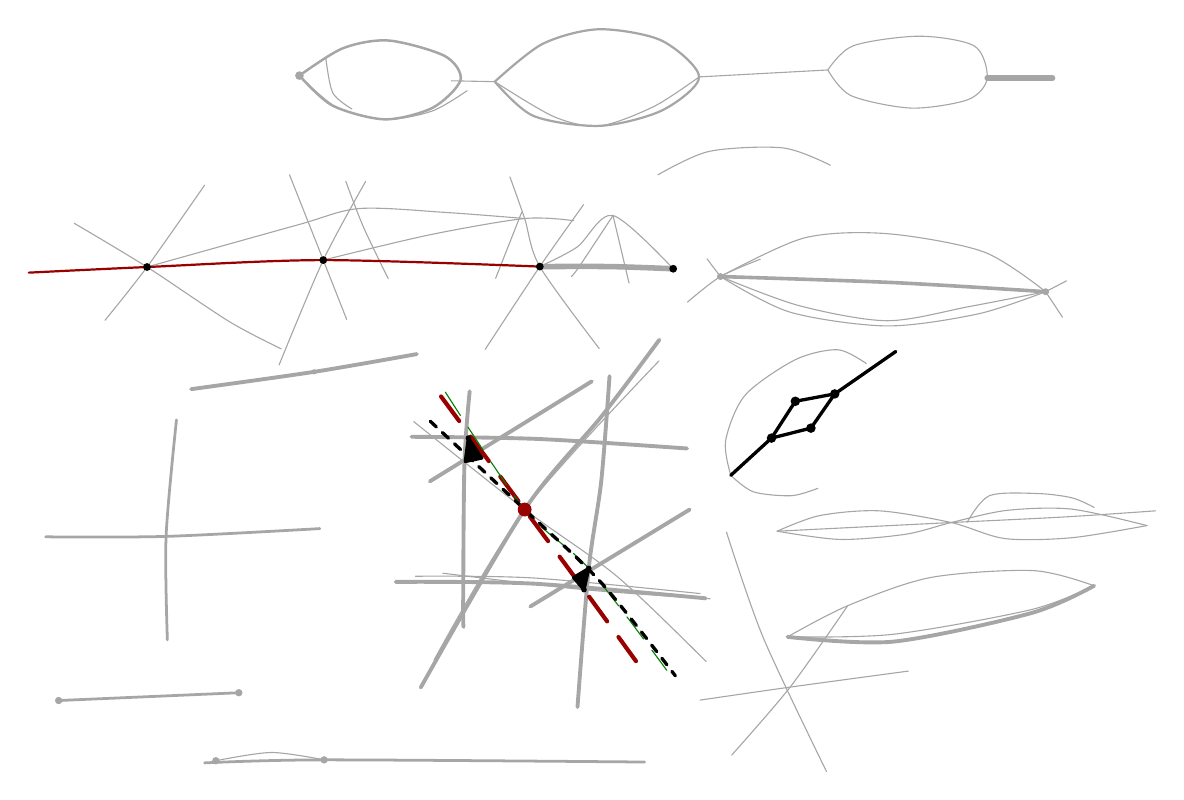
\begin{tikzpicture}[x=.55cm,y=-.55cm,line cap=round,line join=round,g/.style={olive!80!yellow,line width=1.7pt},r/.style={orange!80!brown,line width=1.8pt},w/.style={red!60!black,line width=1.5pt},b/.style={blue!60!black,line width=1.4pt},p/.style={gray!70,thin},k/.style={black,line width=1.2pt},every node/.style={font=\scriptsize}]
% Upper chain of three pencil loops.
\draw[p,line width=.9pt] plot[smooth] coordinates {(9.72,4.21) (10.72,3.58) (11.78,3.4) (13.08,3.76) (13.44,4.31) (12.8,4.95) (11.69,5.22) (10.48,4.9) (9.72,4.21)};
\draw[p] plot[smooth] coordinates {(9.72,4.21) (10.56,4.93) (11.69,5.22) (12.78,5.03) (13.59,4.56)};
\draw[p] plot[smooth] coordinates {(10.33,3.82) (10.49,4.61) (10.93,4.98)};
\draw[p] plot[smooth] coordinates {(13.23,4.33) (14.23,4.35)};
\draw[p,line width=.8pt] plot[smooth] coordinates {(14.23,4.35) (15.33,3.48) (16.63,3.14) (18.08,3.4) (18.95,4.24) (18.1,5.01) (16.66,5.37) (15.12,5.14) (14.23,4.35)};
\draw[p] plot[smooth] coordinates {(14.23,4.35) (15.6,5.16) (16.66,5.37) (17.91,4.92) (18.95,4.24)};
\draw[p] plot[smooth] coordinates {(18.95,4.24) (21.92,4.08)};
\draw[p] plot[smooth] coordinates {(18.0,6.5) (19.18,5.96) (20.89,5.88) (21.98,6.28)};
\draw[p] plot[smooth] coordinates {(21.92,4.08) (22.51,3.52) (24.04,3.3) (25.31,3.53) (25.6,4.27) (25.17,4.76) (23.85,4.96) (22.45,4.67) (21.92,4.08)};
\draw[p,line width=2pt] plot[smooth] coordinates {(25.6,4.27) (27.11,4.27)};
\fill[p] (9.72,4.21) circle (.1);
% Horizontal line with three marked crossings and pencil detours.
\draw[p] plot[smooth] coordinates {(4.52,7.62) (6.2,8.63) (8.1,9.89) (9.3,10.52)};
\draw[p] plot[smooth] coordinates {(7.53,6.74) (6.2,8.63) (5.23,9.86)};
\draw[p] plot[smooth] coordinates {(9.49,6.5) (10.27,8.47) (10.81,9.84)};
\draw[p] plot[smooth] coordinates {(11.25,6.65) (10.27,8.47) (9.25,10.89)};
\draw[p] plot[smooth] coordinates {(10.79,6.65) (11.19,7.69) (11.77,8.9)};
\draw[p] plot[smooth] coordinates {(14.58,6.55) (14.92,7.51) (15.27,8.62) (16.64,10.51)};
\draw[p] plot[smooth] coordinates {(16.28,7.19) (15.27,8.62) (14.01,10.53)};
\draw[p] plot[smooth] coordinates {(14.85,7.37) (14.25,8.89)};
\draw[p] plot[smooth] coordinates {(15.27,8.62) (16.13,8.17) (16.96,7.44) (18.35,8.67)};
\draw[p] plot[smooth] coordinates {(16.96,7.44) (17.33,9.0)};
\draw[p] plot[smooth] coordinates {(16.96,7.44) (16.18,8.62) (16.0,8.85)};
\draw[p] plot[smooth] coordinates {(6.2,8.63) (9.67,7.66) (11.1,7.28) (13.1,7.37) (14.92,7.51)};
\draw[p] plot[smooth] coordinates {(10.27,8.47) (12.71,7.89) (14.92,7.51) (16.05,7.56)};
\draw[w,line width=.8pt] plot[smooth] coordinates {(3.47,8.76) (6.2,8.63) (10.27,8.47) (15.27,8.62)};
\draw[p,line width=2pt] plot[smooth] coordinates {(15.27,8.62) (16.9,8.62) (18.35,8.67)};
\fill[k] (6.2,8.63) circle (.09);
\fill[k] (10.27,8.47) circle (.09);
\fill[k] (15.27,8.62) circle (.09);
\fill[k] (18.35,8.67) circle (.09);
\draw[p,line width=1.4pt] plot[smooth] coordinates {(7.22,11.45) (10.06,11.05) (12.43,10.64)};
\fill[p] (10.06,11.05) circle (.06);
% Right two-point lens and small parallelogram.
\draw[p] plot[smooth] coordinates {(19.44,8.85) (21.37,7.96) (23.29,7.86) (25.52,8.28) (26.95,9.2)};
\draw[p] plot[smooth] coordinates {(19.44,8.85) (21.04,9.67) (23.29,9.99) (25.4,9.71) (26.95,9.2)};
\draw[p] plot[smooth] coordinates {(19.44,8.85) (21.25,9.52) (23.29,9.87) (25.2,9.54) (26.95,9.2)};
\draw[p] plot[smooth] coordinates {(18.68,9.44) (19.44,8.85) (20.36,8.45)};
\draw[p] plot[smooth] coordinates {(19.13,8.44) (19.44,8.85)};
\draw[p] plot[smooth] coordinates {(26.95,9.2) (27.34,9.79)};
\draw[p] plot[smooth] coordinates {(26.95,9.2) (27.43,8.95)};
\draw[p,line width=1.3pt] plot[smooth] coordinates {(19.44,8.85) (23.45,8.99) (26.95,9.2)};
\fill[p] (19.44,8.85) circle (.08);
\fill[p] (26.95,9.2) circle (.08);
\draw[p] plot[smooth] coordinates {(19.68,13.44) (19.56,12.64) (20.01,11.59) (21.17,10.77) (22.15,10.54) (22.81,10.86)};
\draw[p] plot[smooth] coordinates {(19.68,13.44) (20.2,13.82) (21.08,13.91) (21.69,13.74)};
\draw[k] (19.68,13.44)--(20.62,12.58);
\draw[k] (20.62,12.58)--(21.17,11.73)--(22.08,11.56)--(21.53,12.35)--(20.62,12.58);
\draw[k] (22.08,11.56)--(23.49,10.58);
\fill[k] (20.62,12.58) circle (.11);
\fill[k] (21.17,11.73) circle (.11);
\fill[k] (22.08,11.56) circle (.11);
\fill[k] (21.53,12.35) circle (.11);
% Lower central crossings with red and green dashed paths.
\draw[p,line width=1.4pt] plot[smooth] coordinates {(12.31,12.55) (15.23,12.6) (18.67,12.82)};
\draw[p,line width=1.4pt] plot[smooth] coordinates {(11.94,15.9) (15.1,15.94) (19.1,16.28)};
\draw[p,line width=1.4pt] plot[smooth] coordinates {(13.65,11.5) (13.53,13.16) (13.5,16.43) (13.51,16.94)};
\draw[p,line width=1.4pt] plot[smooth] coordinates {(16.88,11.15) (16.69,13.56) (16.4,15.59) (16.14,18.79)};
\draw[p,line width=1.4pt] plot[smooth] coordinates {(12.52,18.34) (14.92,14.23) (16.71,12.06) (18.03,10.31)};
\draw[p,line width=1.4pt] plot[smooth] coordinates {(12.73,13.58) (16.47,11.27)};
\draw[p,line width=1.4pt] plot[smooth] coordinates {(15.05,16.47) (18.73,14.23)};
\draw[p] plot[smooth] coordinates {(12.36,12.2) (14.92,14.23) (17.06,15.78) (19.11,17.74)};
\draw[p] plot[smooth] coordinates {(12.83,17.7) (14.92,14.23) (18.02,10.8)};
\draw[p] plot[smooth] coordinates {(13.03,15.7) (16.29,16.08) (19.2,16.29)};
\draw[p] plot[smooth] coordinates {(12.4,15.77) (15.12,15.81) (18.97,16.17)};
\draw[w,dash pattern=on 11pt off 7pt] plot[smooth] coordinates {(12.99,11.62) (14.92,14.23) (16.29,16.08) (17.49,17.73)};
\draw[green!50!black,dash pattern=on 10pt off 5pt] plot[smooth] coordinates {(13.09,11.52) (14.92,14.23) (16.4,15.59) (18.2,17.94)};
\draw[k,dashed] plot[smooth] coordinates {(12.74,12.19) (14.92,14.23) (16.68,15.91) (18.4,18.07)};
\fill[k] (13.62,12.58) circle (.065);
\fill[k] (13.7,12.98) circle (.065);
\fill[k] (16.4,15.59) circle (.065);
\fill[k] (16.29,16.08) circle (.065);
\fill[w] (14.92,14.23) circle (.16);
\draw[k,fill=black] (13.62,12.58)--(13.93,13.04)--(13.55,13.12)--cycle;
\draw[k,fill=black] (16.4,15.59)--(16.29,16.08)--(16.05,15.8)--cycle;
% Left axes, short segment and two collinear points.
\draw[p,line width=1pt] plot[smooth] coordinates {(6.88,12.16) (6.64,14.85) (6.67,17.24)};
\draw[p,line width=1pt] plot[smooth] coordinates {(3.86,14.86) (6.64,14.85) (10.19,14.67)};
\draw[p,line width=1pt] plot[smooth] coordinates {(4.16,18.64) (8.32,18.46)};
\draw[p,line width=1pt] plot[smooth] coordinates {(7.53,20.08) (10.29,20.01) (17.69,20.06)};
\fill[p] (4.16,18.64) circle (.085);
\fill[p] (8.32,18.46) circle (.085);
\fill[p] (7.79,20.03) circle (.085);
\fill[p] (10.29,20.01) circle (.085);
\draw[p] plot[smooth] coordinates {(7.79,20.03) (9.07,19.84) (10.29,20.01)};
% Right long narrow loops and lower construction.
\draw[p] plot[smooth] coordinates {(20.75,14.73) (21.73,14.37) (23.11,14.26) (24.77,14.53) (26.01,14.9) (27.56,14.88) (29.29,14.6)};
\draw[p] plot[smooth] coordinates {(20.75,14.73) (22.2,14.92) (23.72,14.8) (24.77,14.53) (26.05,14.25) (27.55,14.22) (29.29,14.6)};
\draw[p] plot[smooth] coordinates {(20.75,14.73) (24.77,14.53) (27.4,14.4) (29.49,14.26)};
\draw[p] plot[smooth] coordinates {(25.14,14.52) (25.65,13.91) (26.76,13.86) (27.56,13.96) (28.07,14.18)};
\draw[p] plot[smooth] coordinates {(20.99,17.17) (22.38,16.45) (24.29,15.8) (26.67,15.64) (28.07,15.99)};
\draw[p] plot[smooth] coordinates {(20.99,17.17) (23.43,17.11) (26.62,16.54) (28.07,15.99)};
\draw[p] plot[smooth] coordinates {(19.58,14.75) (20.43,17.19) (21.89,20.28)};
\draw[p] plot[smooth] coordinates {(19.7,19.9) (21.05,18.33) (22.38,16.45)};
\draw[p] plot[smooth] coordinates {(18.97,18.63) (21.05,18.33) (23.78,17.96)};
\draw[p,line width=1.4pt] plot[smooth] coordinates {(20.99,17.17) (23.43,17.28) (26.62,16.62) (28.07,15.99)};
\end{tikzpicture}}
\margin{\mspage{149}}

\scanpage{151}
$\underline{\Sigma}=(X,\Sigma)$, d'où surface cellulaire des positions relatives $X^*=\operatorname{Rel}(\underline{\Sigma})$.

Soit un sommet \inserted{$\rho$} de $X^*$, correspondant à une position relative critique \deleted{$\unsure{\Delta}$}$D_{\rho}$, soit $S_{\rho}=D_{\rho}\cap S(\Sigma)$.
\inserted{Une orientation $\unsure{\bar\omega}$ de $X^*$ correspond à une orientation $\bar\omega_{\rho}$ de $D_{\rho}$.}
Alors les \unsure{arcs sort.} de $\rho$ de $X^*$ correspondent aux \deleted{\unsure{somm.}} éléments \inserted{$(s,\omega)$} de $S_{\rho}$, \uline{munis} d'une orientation; \inserted{soit $\vec a_{s,\omega}$ l'arc}.
A un tel couple $(s,\omega)$, correspond la pos. semi-stble $(D_{\rho},s,\omega)$ \deleted{\unsure{orientée}\ \unsure{qui}} ,
\deleted{\unsure{qui provient}\ \unsure{définit l'arc}\ \unsure{dans le voisin}\ \unsure{germes} $(\rho,\unsure{\bar\omega})$ \unsure{correspond. à une} p.r. stble}
à l'arête $a_{s,\omega}$ sous-jacente : $\vec a_{s,\omega}$; soit $\vec b_{s,\omega}$ l'arête duale, orientée de façon que $(\vec a_{s,\omega},\vec b_{s,\omega})$ soit direct pour $\unsure{\bar\omega}$, donc $\vec b_{s,\omega}$ va d'une p.r. \uline{stable} vers une autre -- c'est le passage de la \unsure{générisation} de $D_{s,\omega}$ en $s$ dite ``\unsure{gauche}'' vers la gén. \unsure{vue|dite} \deleted{\unsure{gauche}}\inserted{\uline{droite}}.
\figure{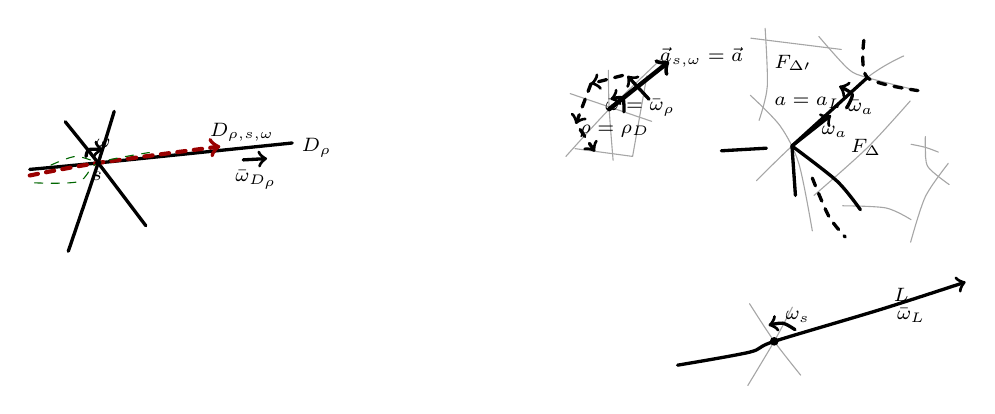
\begin{tikzpicture}[x=.55cm,y=-.55cm,line cap=round,line join=round,g/.style={olive!80!yellow,line width=1.7pt},r/.style={orange!80!brown,line width=1.8pt},w/.style={red!60!black,line width=1.5pt},b/.style={blue!60!black,line width=1.4pt},p/.style={gray!70,thin},k/.style={black,line width=1.2pt},every node/.style={font=\scriptsize}]
% Left local oriented crossing.
\draw[k] plot[smooth] coordinates {(1.43,6.94) (3.01,6.79) (7.49,6.33)};
\draw[k] plot[smooth] coordinates {(2.25,5.84) (3.01,6.79) (4.11,8.24)};
\draw[k] plot[smooth] coordinates {(3.38,5.6) (3.01,6.79) (2.32,8.83)};
\draw[w,dashed,->] plot[smooth] coordinates {(1.43,7.08) (3.01,6.79) (5.83,6.41)};
\draw[green!40!black,dashed] plot[smooth] coordinates {(1.54,7.25) (2.56,7.22) (3.01,6.79) (4.19,6.55)};
\draw[green!40!black,dashed] plot[smooth] coordinates {(1.92,6.84) (2.49,6.64) (3.01,6.79)};
\draw[k,->] plot[smooth] coordinates {(2.73,6.64) (2.8,6.48) (3.12,6.49)};
\draw[k,->] plot[smooth] coordinates {(6.36,6.72) (6.91,6.69)};
\fill[k] (3.01,6.79) circle (.07);
\node at (3.13,6.33) {$\omega$};
\node at (2.98,7.1) {$s$};
\node at (6.33,6.08) {$D_{\unsure{\rho},s,\omega}$};
\node at (8.05,6.44) {$D_\rho$};
\node at (6.66,7.18) {$\bar\omega_{D_\rho}$};
% Central local arrow with orientation and faint construction.
\draw[p] plot[smooth] coordinates {(13.81,6.64) (14.81,5.55) (16.02,4.38)};
\draw[p] plot[smooth] coordinates {(13.91,5.19) (15.79,5.83)};
\draw[p] plot[smooth] coordinates {(14.79,4.65) (14.81,5.55) (14.9,6.73)};
\draw[p] plot[smooth] coordinates {(15.68,4.78) (15.35,6.64)};
\draw[p] plot[smooth] coordinates {(14.02,6.46) (15.35,6.64)};
\draw[k,->,line width=1.6pt] plot[smooth] coordinates {(14.81,5.55) (16.19,4.45)};
\draw[k,->] plot[smooth] coordinates {(15.73,5.32) (15.23,4.78)};
\draw[k,->] plot[smooth] coordinates {(15.15,5.61) (15.12,5.29) (14.84,5.32)};
\draw[k,dashed,->] plot[smooth] coordinates {(15.12,4.77) (14.39,4.96)};
\draw[k,dashed,->] plot[smooth] coordinates {(14.39,4.96) (14.04,5.89)};
\draw[k,dashed,->] plot[smooth] coordinates {(14.14,6.02) (14.48,6.53)};
\node at (16.94,4.35) {$\vec a_{s,\omega}=\vec a$};
\node at (15.52,5.52) {$\bar\omega=\bar\omega_\rho$};
\node at (14.93,6.05) {$\rho=\unsure{\rho_D}$};
% Oriented edge a_L between two face regions.
\draw[p] plot[smooth] coordinates {(18.08,3.91) (20.17,4.17)};
\draw[p] plot[smooth] coordinates {(18.41,3.68) (18.46,5.02) (18.27,5.81)};
\draw[p] plot[smooth] coordinates {(18.07,5.23) (18.76,5.94) (19.19,6.81) (19.5,8.36)};
\draw[p] plot[smooth] coordinates {(19.65,3.87) (20.33,4.62) (20.77,4.82) (21.94,5.12)};
\draw[p] plot[smooth] coordinates {(18.21,7.2) (19.03,6.4) (20.77,4.82) (21.61,4.32)};
\draw[p] plot[smooth] coordinates {(19.54,7.54) (20.77,6.44) (21.76,5.36)};
\draw[p] plot[smooth] coordinates {(20.2,7.78) (21.2,7.83) (21.78,8.1)};
\draw[p] plot[smooth] coordinates {(21.77,8.62) (22.11,7.57) (22.64,6.8)};
\draw[p] plot[smooth] coordinates {(21.78,6.36) (22.11,6.43) (22.41,6.54)};
\draw[p] plot[smooth] coordinates {(22.11,6.18) (22.11,6.43) (22.17,6.88) (22.66,7.29)};
\draw[k] plot[smooth] coordinates {(19.03,6.4) (20.77,4.82)};
\draw[k] plot[smooth] coordinates {(19.03,6.4) (19.11,7.54)};
\draw[k] plot[smooth] coordinates {(19.03,6.4) (20.07,7.21) (20.61,7.87)};
\draw[k] plot[smooth] coordinates {(17.4,6.51) (18.44,6.45)};
\draw[k,dashed] plot[smooth] coordinates {(20.69,3.96) (20.77,4.82) (21.94,5.12)};
\draw[k,dashed] plot[smooth] coordinates {(19.5,7.14) (19.88,8.02) (20.26,8.5)};
\draw[k,->] plot[smooth] coordinates {(19.03,6.4) (19.93,5.69)};
\draw[k,->] plot[smooth] coordinates {(20.29,5.52) (20.42,5.21) (20.12,5.02)};
\node at (19.05,4.48) {$F_{\Delta\prime}$};
\node at (20.74,6.43) {$F_{\Delta}$};
\node at (19.41,5.4) {$a=a_L$};
\node at (20.62,5.51) {$\bar\omega_a$};
\node at (20.01,6.07) {$\omega_a$};
% Oriented L with point s and local rotation omega_s.
\draw[p] plot[smooth] coordinates {(18.05,10.04) (18.62,10.91) (19.23,11.69)};
\draw[p] plot[smooth] coordinates {(19.04,10.12) (18.62,10.91) (18.01,11.93)};
\draw[k,->] plot[smooth] coordinates {(16.39,11.46) (18.05,11.16) (18.62,10.91) (21.09,10.17) (23.04,9.54)};
\draw[k,->] plot[smooth] coordinates {(19.1,10.64) (18.82,10.49) (18.49,10.54)};
\fill[k] (18.62,10.91) circle (.1);
\node at (19.16,10.34) {$\omega_s$};
\node at (21.55,9.84) {$L$};
\node at (21.78,10.32) {$\bar\omega_L$};
\end{tikzpicture}}

La difficulté conceptuelle n'est pas dans l'étude locale de $X^*$ en \unsure{un vois.} de $\rho$, en termes de $D$, mais dans l'étude locale de $X^*$ au voisinage d'une face, correspondant à une p.r. stble $\Delta$, mais dans la description de $X^*$ au voisinage d'une \uline{arête} \inserted{$a_L$}, correspondant à une position r. semi-stble donnée, soit $L$.
Il n'y a pas non plus de difficulté : \unsure{saisir} les faces incidentes \deleted{\unsure{la face} $F$} à $a_L$, et leur circuit des arêtes (contenant $a_L$), mais par contre : saisir les deux \inserted{(?)} sommets incidents à $a_L$.

Notons que la donnée d'une orientation \unsure{superficielle} le long de $a_L$ revient à celle d'une orientation de $L$, celle d'une orientation de $a_L$ à celle d'une orientation superficielle en le \deleted{point} sommet $s\in S_L$, donc une \uline{rive} de $L$\deleted{$\unsure{\{s\}}$} en $s$ revient à celle d'une rive de $a$ i.e. d'une des faces incidentes \unsure{à a}.

Il s'agirait donc, en termes de $(L,\omega_s)$, de reconstruire le sommet extrémité de $\vec a=(a,\omega_a)$, \deleted{\unsure{dans des termes}} si possible en termes d'une position relative critique, déduite de $L$ par ``blocage'' autour de $s$, dans le sens indiqué par l'orientation $\omega_s$ en $\uline{s}$, i.e. par la rive correspondante de $L-\{s\}$.
L'ennui, c'est qu'il y a plusieurs choix naturels qui viennent à l'esprit, et qu'il n'est pas sûr qu'aucun de ces choix ne marche!

{\ttfamily\unsure{//** CRAY6 0013 - O}}
\unsure{{\scriptsize\begin{tabular}{l}
\texttt{\ CCCCCCCCCC\ \ \ RRRRRRRRRRR\ \ \ AAAAAAAAAA\ \ \ YY\ \ \ \ \ \ \ \ YY\ \ \ 6666666666}\\
\texttt{CCCCCCCCCCCC\ \ RRRRRRRRRRRR\ AAAAAAAAAAAA\ \ YY\ \ \ \ \ \ \ \ YY\ \ 666666666666}\\
\texttt{CC\ \ \ \ \ \ \ \ CC\ \ RR\ \ \ \ \ \ \ \ RR\ AA\ \ \ \ \ \ \ \ AA\ \ YY\ \ \ \ \ \ YY\ \ \ 66\ \ \ \ \ \ \ \ 66}\\
\texttt{CC\ \ \ \ \ \ \ \ \ \ \ \ RR\ \ \ \ \ \ \ \ RR\ AA\ \ \ \ \ \ \ \ AA\ \ \ YY\ \ \ \ YY\ \ \ \ 66}\\
\texttt{CC\ \ \ \ \ \ \ \ \ \ \ \ RR\ \ \ \ \ \ \ \ RR\ AA\ \ \ \ \ \ \ \ AA\ \ \ \ YY\ \ YY\ \ \ \ \ 66}\\
\texttt{CC\ \ \ \ \ \ \ \ \ \ \ \ RRRRRRRRRRRR\ AAAAAAAAAAAA\ \ \ \ \ YYYY\ \ \ \ \ \ 66666666666}\\
\texttt{CC\ \ \ \ \ \ \ \ \ \ \ \ RRRRRRRRRRR\ \ AAAAAAAAAAAA\ \ \ \ \ \ YY\ \ \ \ \ \ \ 666666666666}\\
\texttt{CC\ \ \ \ \ \ \ \ \ \ \ \ RR\ \ \ \ RR\ \ \ \ \ AA\ \ \ \ \ \ \ \ AA\ \ \ \ \ \ YY\ \ \ \ \ \ \ 66\ \ \ \ \ \ \ \ 66}\\
\texttt{CC\ \ \ \ \ \ \ \ \ \ \ \ RR\ \ \ \ \ RR\ \ \ \ AA\ \ \ \ \ \ \ \ AA\ \ \ \ \ \ YY\ \ \ \ \ \ \ 66\ \ \ \ \ \ \ \ 66}\\
\texttt{CC\ \ \ \ \ \ \ \ CC\ \ RR\ \ \ \ \ \ RR\ \ \ AA\ \ \ \ \ \ \ \ AA\ \ \ \ \ \ YY\ \ \ \ \ \ \ 66\ \ \ \ \ \ \ \ 66}\\
\texttt{CCCCCCCCCCCC\ \ RR\ \ \ \ \ \ \ RR\ \ AA\ \ \ \ \ \ \ \ AA\ \ \ \ \ \ YY\ \ \ \ \ \ \ 666666666666}\\
\texttt{\ CCCCCCCCCC\ \ \ RR\ \ \ \ \ \ \ \ RR\ AA\ \ \ \ \ \ \ \ AA\ \ \ \ \ \ YY\ \ \ \ \ \ \ \ 6666666666}\\
\end{tabular}}}
{\ttfamily ****A\quad END\quad JOB\quad13\quad CRAY6\quad- CRAY OUTPUT -\quad ROOM\quad3.24.18 PM 19 AUG 82\quad R6.PR1\quad SYS JES2\quad JOB\quad13\quad END\quad A****}\\
{\ttfamily ****A\quad END\quad JOB\quad13\quad CRAY6\quad- CRAY OUTPUT -\quad ROOM\quad3.24.18 PM 19 AUG 82\quad R6.PR1\quad SYS JES2\quad JOB\quad13\quad END\quad A****}\\
{\ttfamily ****A\quad END\quad JOB\quad13\quad CRAY6\quad- CRAY OUTPUT -\quad ROOM\quad3.24.18 PM 19 AUG 82\quad R6.PR1\quad SYS JES2\quad JOB\quad13\quad END\quad A****}\\
{\ttfamily ****A\quad END\quad JOB\quad13\quad CRAY6\quad- CRAY OUTPUT -\quad ROOM\quad3.24.18 PM 19 AUG 82\quad R6.PR1\quad SYS JES2\quad JOB\quad13\quad END\quad A****}\\
{\ttfamily ****A\quad END\quad JOB\quad13\quad CRAY6\quad- CRAY OUTPUT -\quad ROOM\quad3.24.18 PM 19 AUG 82\quad R6.PR1\quad SYS JES2\quad JOB\quad13\quad END\quad A****}\\
{\ttfamily ****A\quad END\quad JOB\quad13\quad CRAY6\quad- CRAY OUTPUT -\quad ROOM\quad3.24.18 PM 19 AUG 82\quad R6.PR1\quad SYS JES2\quad JOB\quad13\quad END\quad A****}\\
\margin{\mspage{150}}

\scanpage{152}
{\ttfamily //*\quad CRAY6\quad0013\quad-\quad CRAY\unsure{6}}
{\scriptsize\begin{tabular}{l}
\texttt{\ CCCCCCCCCC\ \ \ RRRRRRRRRRR\ \ \ AAAAAAAAAA\ \ \ YY\ \ \ \ \ \ \ \ YY\ \ \ 6666666666}\\
\texttt{CCCCCCCCCCCC\ \ RRRRRRRRRRRR\ AAAAAAAAAAAA\ \ YY\ \ \ \ \ \ \ \ YY\ \ 666666666666}\\
\texttt{CC\ \ \ \ \ \ \ \ CC\ \ RR\ \ \ \ \ \ \ \ RR\ AA\ \ \ \ \ \ \ \ AA\ \ YY\ \ \ \ \ \ YY\ \ \ 66\ \ \ \ \ \ \ \ 66}\\
\texttt{CC\ \ \ \ \ \ \ \ \ \ \ \ RR\ \ \ \ \ \ \ \ RR\ AA\ \ \ \ \ \ \ \ AA\ \ \ YY\ \ \ \ YY\ \ \ \ 66}\\
\texttt{CC\ \ \ \ \ \ \ \ \ \ \ \ RR\ \ \ \ \ \ \ \ RR\ AA\ \ \ \ \ \ \ \ AA\ \ \ \ YY\ \ YY\ \ \ \ \ 66}\\
\texttt{CC\ \ \ \ \ \ \ \ \ \ \ \ RRRRRRRRRRRR\ AAAAAAAAAAAA\ \ \ \ \ YYYY\ \ \ \ \ \ 66666666666}\\
\texttt{CC\ \ \ \ \ \ \ \ \ \ \ \ RRRRRRRRRRR\ \ AAAAAAAAAAAA\ \ \ \ \ \ YY\ \ \ \ \ \ \ 666666666666}\\
\texttt{CC\ \ \ \ \ \ \ \ \ \ \ \ RR\ \ \ \ RR\ \ \ \ \ AA\ \ \ \ \ \ \ \ AA\ \ \ \ \ \ YY\ \ \ \ \ \ \ 66\ \ \ \ \ \ \ \ 66}\\
\texttt{CC\ \ \ \ \ \ \ \ \ \ \ \ RR\ \ \ \ \ RR\ \ \ \ AA\ \ \ \ \ \ \ \ AA\ \ \ \ \ \ YY\ \ \ \ \ \ \ 66\ \ \ \ \ \ \ \ 66}\\
\texttt{CC\ \ \ \ \ \ \ \ CC\ \ RR\ \ \ \ \ \ RR\ \ \ AA\ \ \ \ \ \ \ \ AA\ \ \ \ \ \ YY\ \ \ \ \ \ \ 66\ \ \ \ \ \ \ \ 66}\\
\texttt{CCCCCCCCCCCC\ \ RR\ \ \ \ \ \ \ RR\ \ AA\ \ \ \ \ \ \ \ AA\ \ \ \ \ \ YY\ \ \ \ \ \ \ 666666666666}\\
\texttt{\ CCCCCCCCCC\ \ \ RR\ \ \ \ \ \ \ \ RR\ AA\ \ \ \ \ \ \ \ AA\ \ \ \ \ \ YY\ \ \ \ \ \ \ \ 6666666666}\\
\end{tabular}}
{\ttfamily ****A\quad END\quad JOB\quad13\quad CRAY6\quad- CRAY OUTPUT -\quad ROOM\quad3.24.18 PM 19 AUG 82\quad R6.PR1\quad SYS JES2\quad JOB\quad13\quad END\quad A****}\\
{\ttfamily ****A\quad END\quad JOB\quad13\quad CRAY6\quad- CRAY OUTPUT -\quad ROOM\quad3.24.18 PM 19 AUG 82\quad R6.PR1\quad SYS JES2\quad JOB\quad13\quad END\quad A****}\\
{\ttfamily ****A\quad END\quad JOB\quad13\quad CRAY6\quad- CRAY OUTPUT -\quad ROOM\quad3.24.18 PM 19 AUG 82\quad R6.PR1\quad SYS JES2\quad JOB\quad13\quad END\quad A****}\\
{\ttfamily ****A\quad END\quad JOB\quad13\quad CRAY6\quad- CRAY OUTPUT -\quad ROOM\quad3.24.18 PM 19 AUG 82\quad R6.PR1\quad SYS JES2\quad JOB\quad13\quad END\quad A****}\\
{\ttfamily ****A\quad END\quad JOB\quad13\quad CRAY6\quad- CRAY OUTPUT -\quad ROOM\quad3.24.18 PM 19 AUG 82\quad R6.PR1\quad SYS JES2\quad JOB\quad13\quad END\quad A****}\\
{\ttfamily ****A\quad END\quad JOB\quad13\quad CRAY6\quad- CRAY OUTPUT -\quad ROOM\quad3.24.18 PM 19 AUG 82\quad R6.PR1\quad SYS JES2\quad JOB\quad13\quad END\quad A****}\\
\figure{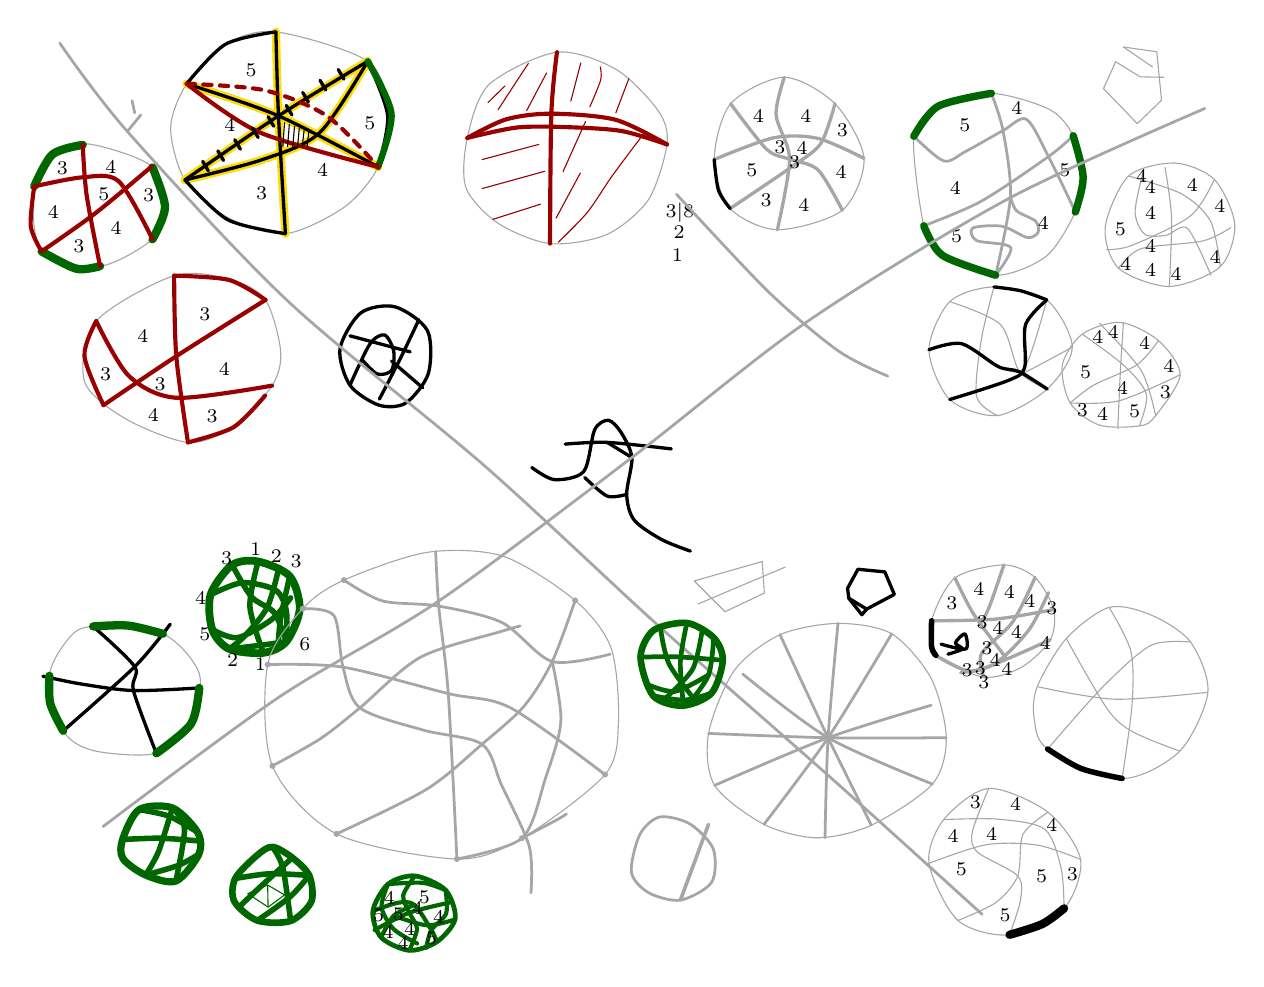
\begin{tikzpicture}[x=.55cm,y=-.55cm,line cap=round,line join=round,g/.style={olive!80!yellow,line width=1.7pt},r/.style={orange!80!brown,line width=1.8pt},w/.style={red!60!black,line width=1.5pt},b/.style={blue!60!black,line width=1.4pt},p/.style={gray!70,thin},k/.style={black,line width=1.2pt},every node/.style={font=\scriptsize}]
% Upper-left three coloured arrangements.
\draw[p] plot[smooth cycle] coordinates {(1.23,4.4) (1.82,3.5) (2.66,3.45) (3.94,3.94) (4.23,4.92) (3.96,5.62) (2.75,6.24) (1.4,5.9)};
\draw[green!40!black,line width=3pt] plot[smooth] coordinates {(1.23,4.4) (1.65,3.66) (2.35,3.44)};
\draw[green!40!black,line width=3pt] plot[smooth] coordinates {(1.4,5.9) (2.2,6.3) (2.75,6.24)};
\draw[green!40!black,line width=3pt] plot[smooth] coordinates {(3.96,3.96) (4.25,4.88) (3.96,5.62)};
\draw[w] plot[smooth] coordinates {(1.23,4.4) (2.34,4.19) (3.18,4.28) (3.96,5.62)};
\draw[w] plot[smooth] coordinates {(2.35,3.44) (2.44,4.6) (2.75,6.24)};
\draw[w] plot[smooth] coordinates {(1.4,5.9) (2.64,5.02) (3.94,3.94)};
\draw[w] plot[smooth] coordinates {(1.4,5.9) (1.15,5.32) (1.23,4.4)};
\node at (1.88,3.97) {$3$};
\node at (3.0,3.95) {$4$};
\node at (2.84,4.58) {$5$};
\node at (3.87,4.61) {$3$};
\node at (1.67,4.99) {$4$};
\node at (3.12,5.37) {$4$};
\node at (2.26,5.79) {$3$};
\draw[p] plot[smooth cycle] coordinates {(4.75,2.03) (5.64,1.12) (6.81,.83) (8.93,1.51) (9.43,2.71) (9.17,3.95) (8.4,4.87) (7.03,5.49) (5.68,5.11) (4.71,4.25) (4.38,3.05)};
\draw[yellow!80!orange,line width=3pt] plot[smooth] coordinates {(4.75,2.03) (6.87,2.77) (9.17,3.95)};
\draw[yellow!80!orange,line width=3pt] plot[smooth] coordinates {(4.71,4.25) (6.87,2.77) (8.93,1.51)};
\draw[yellow!80!orange,line width=3pt] plot[smooth] coordinates {(6.81,.83) (6.87,2.77) (7.03,5.49)};
\draw[yellow!80!orange,line width=3pt] plot[smooth] coordinates {(4.71,4.25) (6.5,3.78) (7.82,3.16) (8.93,1.51)};
\draw[k] plot[smooth] coordinates {(4.75,2.03) (5.64,1.12) (6.81,.83)};
\draw[k] plot[smooth] coordinates {(4.75,2.03) (6.87,2.77) (9.17,3.95)};
\draw[k] plot[smooth] coordinates {(4.71,4.25) (6.87,2.77) (8.93,1.51)};
\draw[k] plot[smooth] coordinates {(6.81,.83) (6.87,2.77) (7.03,5.49)};
\draw[k] plot[smooth] coordinates {(4.71,4.25) (6.5,3.78) (7.82,3.16) (8.93,1.51)};
\draw[k] plot[smooth] coordinates {(4.71,4.25) (5.7,5.17) (7.03,5.49)};
\draw[k] plot[smooth] coordinates {(8.93,1.51) (9.39,2.76) (9.17,3.95)};
\draw[green!40!black,line width=2.3pt] plot[smooth] coordinates {(8.93,1.51) (9.48,2.72) (9.17,3.95)};
\draw[w] plot[smooth] coordinates {(4.75,2.03) (6.43,3.15) (9.17,3.95)};
\draw[w,dashed] plot[smooth] coordinates {(4.75,2.03) (6.55,2.18) (8.0,2.78) (9.17,3.95)};
\draw[k] (5.12,3.82)--(5.25,4.04);
\draw[k] (5.47,3.58)--(5.6,3.8000000000000003);
\draw[k] (5.86,3.32)--(5.99,3.54);
\draw[k] (6.2700000000000005,3.05)--(6.4,3.27);
\draw[k] (6.63,2.79)--(6.76,3.0100000000000002);
\draw[k] (7.05,2.53)--(7.18,2.75);
\draw[k] (7.430000000000001,2.23)--(7.5600000000000005,2.45);
\draw[k] (7.83,1.9499999999999997)--(7.96,2.17);
\draw[k] (8.25,1.7000000000000002)--(8.38,1.9200000000000002);
\draw[k,thin] (7.01,2.93)--(6.97,3.48);
\draw[k,thin] (7.12,2.97)--(7.08,3.48);
\draw[k,thin] (7.24,3.01)--(7.2,3.48);
\draw[k,thin] (7.35,3.06)--(7.31,3.48);
\draw[k,thin] (7.46,3.11)--(7.42,3.48);
\draw[k,thin] (7.57,3.14)--(7.53,3.48);
\node at (6.24,1.72) {$5$};
\node at (5.75,2.98) {$4$};
\node at (6.48,4.56) {$3$};
\node at (7.89,4.03) {$4$};
\node at (8.98,2.94) {$5$};
\draw[p] plot[smooth cycle] coordinates {(2.66,7.51) (4.46,6.46) (5.76,6.55) (6.57,7.02) (6.92,8.21) (6.72,9.0) (5.8,9.96) (4.78,10.31) (3.33,9.76) (2.39,8.9)};
\draw[w] plot[smooth] coordinates {(2.66,7.51) (2.39,8.32) (2.83,9.45)};
\draw[w] plot[smooth] coordinates {(4.46,6.46) (5.73,6.56) (6.57,7.02)};
\draw[w] plot[smooth] coordinates {(4.46,6.46) (4.51,8.32) (4.78,10.31)};
\draw[w] plot[smooth] coordinates {(2.83,9.45) (4.51,8.32) (6.57,7.02)};
\draw[w] plot[smooth] coordinates {(2.66,7.51) (3.41,8.77) (4.51,9.28) (6.72,9.0)};
\draw[w] plot[smooth] coordinates {(4.78,10.31) (5.83,9.96) (6.56,9.23)};
\node at (3.74,7.85) {$4$};
\node at (5.17,7.35) {$3$};
\node at (5.62,8.62) {$4$};
\node at (5.34,9.7) {$3$};
\node at (3.98,9.69) {$4$};
\node at (2.88,8.74) {$3$};
\node at (4.14,8.96) {$3$};
% Upper-middle hemisphere and hatched meridian.
\draw[p] plot[smooth cycle] coordinates {(11.23,3.28) (11.73,2.05) (13.3,1.3) (14.67,1.7) (15.65,2.67) (15.84,3.43) (15.41,4.71) (14.45,5.51) (13.14,5.72) (11.94,5.25) (11.2,4.43)};
\draw[w] plot[smooth] coordinates {(13.3,1.3) (13.17,2.72) (13.14,5.72)};
\draw[w] plot[smooth] coordinates {(11.23,3.28) (12.13,2.85) (13.17,2.72) (14.65,2.86) (15.84,3.43)};
\draw[w] plot[smooth] coordinates {(11.23,3.28) (12.37,3.04) (13.5,3.03) (14.79,3.12) (15.84,3.43)};
\draw[w,thin] plot[smooth] coordinates {(11.71,2.46) (12.1,2.08)};
\draw[w,thin] plot[smooth] coordinates {(11.94,2.63) (12.35,2.0) (12.64,1.56)};
\draw[w,thin] plot[smooth] coordinates {(12.6,2.65) (13.06,1.78)};
\draw[w,thin] plot[smooth] coordinates {(13.62,2.43) (13.85,1.55)};
\draw[w,thin] plot[smooth] coordinates {(14.06,2.56) (14.31,1.94) (14.3,1.64)};
\draw[w,thin] plot[smooth] coordinates {(14.66,2.7) (14.96,1.91)};
\draw[w,thin] plot[smooth] coordinates {(11.57,3.78) (12.88,3.43)};
\draw[w,thin] plot[smooth] coordinates {(11.57,4.45) (13.02,4.05)};
\draw[w,thin] plot[smooth] coordinates {(11.82,5.16) (12.92,4.81)};
\draw[w,thin] plot[smooth] coordinates {(13.44,4.06) (13.96,2.9)};
\draw[w,thin] plot[smooth] coordinates {(13.28,5.13) (13.84,4.09)};
\draw[w,thin] plot[smooth] coordinates {(13.33,5.69) (14.0,5.0) (14.58,4.15) (15.32,3.16)};
\fill[w] (13.17,2.72) circle (.07);
% Upper-right five small arrangements and polygon sketch.
\draw[p] plot[smooth cycle] coordinates {(16.93,3.78) (17.31,2.49) (18.55,1.88) (19.72,2.49) (20.39,3.75) (19.89,4.95) (18.39,5.4) (17.3,4.91)};
\draw[p,line width=1.2pt] plot[smooth] coordinates {(18.55,1.88) (18.36,2.75) (18.67,3.77) (18.39,5.4)};
\draw[p,line width=1.2pt] plot[smooth] coordinates {(17.31,2.49) (18.14,3.54) (18.67,3.77) (19.33,4.02) (19.89,4.95)};
\draw[p,line width=1.2pt] plot[smooth] coordinates {(19.72,2.49) (19.39,3.41) (18.73,3.94) (17.3,4.91)};
\draw[p,line width=1.2pt] plot[smooth] coordinates {(16.93,3.78) (18.29,3.28) (19.32,3.29) (20.39,3.75)};
\draw[k] plot[smooth] coordinates {(16.93,3.78) (17.03,4.49) (17.3,4.91)};
\node at (17.95,2.78) {$4$};
\node at (19.05,2.79) {$4$};
\node at (19.89,3.11) {$3$};
\node at (19.86,4.07) {$4$};
\node at (19.0,4.83) {$4$};
\node at (18.13,4.73) {$3$};
\node at (17.8,4.02) {$5$};
\node at (18.45,3.49) {$3$};
\node at (18.96,3.52) {$4$};
\node at (18.79,3.84) {$\unsure{3}$};
\draw[p] plot[smooth cycle] coordinates {(21.54,3.24) (22.1,2.55) (23.33,2.25) (24.67,2.62) (25.22,3.23) (25.45,4.19) (25.27,4.99) (24.6,6.01) (23.43,6.45) (22.17,5.92) (21.77,5.31)};
\draw[p,line width=1pt] plot[smooth] coordinates {(23.33,2.25) (23.6,3.11) (23.77,4.63) (23.43,6.45)};
\draw[p,line width=1pt] plot[smooth] coordinates {(21.54,3.24) (22.23,3.81) (22.74,3.59) (23.6,3.11) (24.14,2.85) (24.65,3.71) (25.27,4.99)};
\draw[p,line width=1pt] plot[smooth] coordinates {(21.77,5.31) (23.1,4.74) (24.65,3.71) (25.22,3.23)};
\draw[p,line width=1pt] plot[smooth] coordinates {(23.77,4.63) (23.91,4.96) (24.35,5.2) (24.41,5.46) (24.16,5.58) (23.58,5.32) (22.9,5.36) (22.99,5.65) (23.78,5.81) (23.43,6.45)};
\draw[green!40!black,line width=2.7pt] plot[smooth] coordinates {(21.54,3.24) (22.1,2.55) (23.33,2.25)};
\draw[green!40!black,line width=2.7pt] plot[smooth] coordinates {(25.22,3.23) (25.45,4.19) (25.27,4.99)};
\draw[green!40!black,line width=2.7pt] plot[smooth] coordinates {(21.77,5.31) (22.2,5.99) (23.43,6.45)};
\node at (22.72,2.98) {$5$};
\node at (23.92,2.59) {$4$};
\node at (25.03,4.03) {$5$};
\node at (24.53,5.24) {$4$};
\node at (22.53,5.55) {$5$};
\node at (22.5,4.45) {$4$};
\draw[p] (26.38,1.18)--(27.15,1.29)--(27.26,2.41)--(26.7,2.95)--(25.92,2.14)--(26.2,1.52)--(26.77,1.87)--(27.31,1.88);
\draw[p] (26.38,1.18)--(27.05,1.64);
\draw[p] plot[smooth cycle] coordinates {(26.5,4.16) (27.57,3.86) (28.48,4.24) (28.95,5.27) (28.62,6.25) (27.44,6.71) (26.27,6.29) (25.96,5.34)};
\draw[p] plot[smooth] coordinates {(26.84,4.04) (26.65,4.99) (26.87,5.5) (27.36,5.53) (27.86,5.37) (28.4,6.45)};
\draw[p] plot[smooth] coordinates {(27.34,3.96) (27.49,5.11) (27.44,6.71)};
\draw[p] plot[smooth] coordinates {(26.5,4.16) (27.72,4.57) (28.39,5.2) (28.62,6.25)};
\draw[p] plot[smooth] coordinates {(28.48,4.24) (27.93,5.08) (26.58,5.76) (25.99,5.86)};
\draw[p] plot[smooth] coordinates {(26.27,6.29) (26.78,5.84) (28.21,5.66) (28.86,5.35)};
\node at (26.8,4.17) {$4$};
\node at (27.0,4.43) {$4$};
\node at (27.01,5.01) {$4$};
\node at (27.97,4.38) {$4$};
\node at (28.61,4.86) {$4$};
\node at (26.31,5.39) {$5$};
\node at (27.01,5.78) {$\unsure{4}$};
\node at (26.44,6.19) {$4$};
\node at (27.01,6.34) {$4$};
\node at (27.6,6.43) {$4$};
\node at (28.5,6.03) {$4$};
\draw[p] plot[smooth cycle] coordinates {(22.37,7.06) (23.39,6.72) (24.61,7.02) (25.2,8.11) (24.62,9.08) (23.47,9.69) (22.37,9.32) (21.89,8.17)};
\draw[p] plot[smooth] coordinates {(23.39,6.72) (23.1,7.93) (22.99,9.25) (23.47,9.69)};
\draw[p] plot[smooth] coordinates {(22.37,7.06) (23.54,7.59) (23.98,8.68) (24.62,9.08)};
\draw[p] plot[smooth] coordinates {(21.89,8.17) (22.64,8.03) (23.49,8.56) (24.1,8.58) (24.61,7.02)};
\draw[p] plot[smooth] coordinates {(22.37,9.32) (23.72,8.88) (25.2,8.11)};
\draw[k] plot[smooth] coordinates {(23.39,6.72) (24.01,6.81) (24.61,7.02)};
\draw[k] plot[smooth] coordinates {(24.61,7.02) (24.12,7.59) (24.1,8.58) (23.72,8.88) (22.37,9.32)};
\draw[k] plot[smooth] coordinates {(21.89,8.17) (22.64,8.03) (23.49,8.56) (23.98,8.68) (24.62,9.08)};
\draw[p] plot[smooth cycle] coordinates {(25.43,7.81) (26.31,7.54) (27.19,7.96) (27.69,8.75) (27.11,9.71) (26.75,9.93) (25.82,9.91) (25.15,9.4) (24.97,8.52)};
\draw[p] plot[smooth] coordinates {(25.83,7.56) (26.79,8.65) (27.12,9.68)};
\draw[p] plot[smooth] coordinates {(26.38,7.54) (26.31,8.66) (26.25,10.0)};
\draw[p] plot[smooth] coordinates {(25.43,7.81) (26.4,8.54) (26.91,9.2) (26.75,9.93)};
\draw[p] plot[smooth] coordinates {(27.19,7.96) (26.69,8.52) (25.69,8.99) (25.15,9.4)};
\draw[p] plot[smooth] coordinates {(25.15,9.4) (26.28,9.35) (27.69,8.75)};
\node at (25.79,7.88) {$4$};
\node at (26.15,7.76) {$4$};
\node at (26.87,8.03) {$4$};
\node at (27.43,8.56) {$4$};
\node at (25.51,8.68) {$5$};
\node at (26.36,9.06) {$4$};
\node at (27.35,9.15) {$3$};
\node at (25.43,9.57) {$3$};
\node at (25.9,9.67) {$4$};
\node at (26.64,9.59) {$5$};
\node at (16.14,5.01) {$\unsure{3|8}$};
\node at (16.12,5.46) {$2$};
\node at (16.08,5.99) {$1$};
% Two middle unlabelled ink studies and long crossing strokes.
\draw[k] plot[smooth cycle] coordinates {(8.52,8.99) (8.29,8.15) (8.77,7.32) (9.56,7.18) (10.31,7.73) (10.33,8.72) (9.81,9.4) (9.19,9.45)};
\draw[k] plot[smooth] coordinates {(8.52,8.99) (8.98,8.04) (9.32,7.83) (9.53,8.2) (9.48,8.65) (9.15,8.73) (8.81,8.41)};
\draw[k] plot[smooth] coordinates {(9.2,9.31) (9.7,8.34) (10.11,7.48)};
\draw[k] plot[smooth] coordinates {(8.52,7.85) (9.91,8.22)};
\draw[k] plot[smooth] coordinates {(9.48,8.43) (10.2,9.05)};
\draw[k] plot[smooth] coordinates {(12.72,10.89) (13.24,11.17) (13.92,10.98) (14.17,10.02) (14.49,9.8) (14.78,10.08) (15.03,10.66) (14.91,11.51) (15.08,12.1) (15.71,12.55) (16.38,12.82)};
\draw[k] plot[smooth] coordinates {(13.49,10.35) (14.46,10.31) (15.94,10.46)};
\draw[k] plot[smooth] coordinates {(13.94,11.12) (14.46,11.55) (14.91,11.51)};
\draw[k] plot[smooth] coordinates {(14.46,10.31) (15.03,10.66)};
\draw[p,line width=1pt] plot[smooth] coordinates {(1.82,1.09) (3.38,3.13) (7.1,7.06) (11.65,10.87) (15.65,14.55) (19.71,18.13) (23.12,21.21)};
\draw[p,line width=1pt] plot[smooth] coordinates {(2.82,19.18) (6.87,16.2) (10.56,13.98) (15.03,10.66) (19.08,7.52) (23.73,4.68) (28.26,2.6)};
\draw[p,line width=1pt] plot[smooth] coordinates {(3.49,2.42) (3.55,2.7)};
\draw[p,line width=1pt] plot[smooth] coordinates {(3.38,3.13) (3.69,2.75)};
\draw[p,line width=1pt] plot[smooth] coordinates {(16.06,4.58) (18.18,6.83) (19.8,8.2) (20.94,8.78)};
% Lower left oval and small green numbered arrangement.
\draw[p] plot[smooth cycle] coordinates {(1.58,15.7) (2.04,14.82) (2.59,14.56) (4.2,14.73) (5.04,15.65) (4.85,16.81) (4.05,17.49) (2.61,17.43) (1.9,16.97)};
\draw[k] plot[smooth] coordinates {(2.59,14.56) (3.55,15.49) (3.52,16.04) (4.05,17.49)};
\draw[k] plot[smooth] coordinates {(4.37,14.51) (3.55,15.49) (1.9,16.97)};
\draw[k] plot[smooth] coordinates {(1.43,15.71) (2.32,15.89) (3.52,16.04) (5.04,15.98)};
\draw[green!40!black,line width=3pt] plot[smooth] coordinates {(2.59,14.56) (3.4,14.54) (4.2,14.73)};
\draw[green!40!black,line width=3pt] plot[smooth] coordinates {(1.58,15.7) (1.6,16.34) (1.9,16.97)};
\draw[green!40!black,line width=3pt] plot[smooth] coordinates {(4.05,17.49) (4.85,16.81) (5.04,15.98)};
\draw[green!40!black,line width=2.8pt] plot[smooth cycle] coordinates {(5.3,13.83) (5.8,13.14) (6.4,13.06) (7.13,13.4) (7.36,14.16) (7.05,14.91) (6.52,15.17) (5.73,15.08) (5.34,14.63)};
\draw[green!40!black,line width=2pt] plot[smooth] coordinates {(5.8,13.14) (6.25,13.88) (6.77,14.24) (7.05,14.91)};
\draw[green!40!black,line width=2pt] plot[smooth] coordinates {(6.4,13.06) (6.21,14.1) (6.52,15.17)};
\draw[green!40!black,line width=2pt] plot[smooth] coordinates {(6.88,13.2) (6.61,14.12) (6.08,14.79) (5.73,15.08)};
\draw[green!40!black,line width=2pt] plot[smooth] coordinates {(7.13,13.4) (6.92,14.37) (6.86,15.03)};
\draw[green!40!black,line width=2pt] plot[smooth] coordinates {(5.3,13.83) (6.03,13.55) (6.8,13.72) (7.05,14.19) (7.05,14.91)};
\draw[green!40!black,line width=2pt] plot[smooth] coordinates {(5.34,14.63) (5.92,14.82) (6.7,14.41) (7.15,13.9)};
\draw[green!40!black,line width=2pt] plot[smooth] coordinates {(5.73,15.08) (6.5,14.99) (7.05,14.91)};
\node at (5.67,12.98) {$3$};
\node at (6.34,12.77) {$1$};
\node at (6.82,12.95) {$2$};
\node at (7.28,13.05) {$3$};
\node at (5.07,13.9) {$4$};
\node at (5.17,14.73) {$5$};
\node at (5.81,15.34) {$2$};
\node at (6.45,15.43) {$1$};
\node at (7.48,14.97) {$\unsure{6}$};
% Large lower central sphere.
\draw[p] plot[smooth cycle] coordinates {(6.62,15.44) (7.43,14.15) (8.38,13.49) (10.3,12.85) (12.06,12.94) (13.72,13.96) (14.55,15.06) (14.72,16.76) (14.41,17.98) (12.49,19.45) (10.99,19.93) (8.21,19.35) (6.73,17.78)};
\draw[p,line width=1pt] plot[smooth] coordinates {(7.43,14.15) (8.15,14.31) (8.36,15.5) (8.75,16.44) (10.2,16.95) (11.57,17.28) (12.02,18.22) (12.66,19.64) (12.7,20.71)};
\draw[p,line width=1pt] plot[smooth] coordinates {(10.5,12.83) (10.57,14.09) (10.79,16.11) (10.99,19.93)};
\draw[p,line width=1pt] plot[smooth] coordinates {(8.38,13.49) (9.27,13.97) (10.57,14.09) (12.03,14.47) (13.19,15.37) (14.53,15.2)};
\draw[p,line width=1pt] plot[smooth] coordinates {(6.62,15.44) (8.36,15.5) (10.79,16.11) (12.23,16.44) (14.41,17.98)};
\draw[p,line width=1pt] plot[smooth] coordinates {(6.73,17.78) (7.84,17.15) (8.75,16.44) (10.15,15.27) (12.03,14.67) (12.45,14.55)};
\draw[p,line width=1pt] plot[smooth] coordinates {(8.21,19.35) (10.29,18.32) (11.57,17.28) (12.54,16.4) (13.19,15.37) (13.72,13.96)};
\draw[p,line width=1pt] plot[smooth] coordinates {(10.99,19.93) (12.49,19.45) (13.03,18.08) (13.39,16.75) (13.19,15.37)};
\draw[p,line width=1pt] plot[smooth] coordinates {(12.49,19.45) (13.29,19.03) (13.52,18.89)};
\fill[p] (6.62,15.44) circle (.07);
\fill[p] (7.43,14.15) circle (.07);
\fill[p] (8.38,13.49) circle (.07);
\fill[p] (13.72,13.96) circle (.07);
\fill[p] (14.41,17.98) circle (.07);
\fill[p] (12.49,19.45) circle (.07);
\fill[p] (10.99,19.93) circle (.07);
\fill[p] (8.21,19.35) circle (.07);
\fill[p] (6.73,17.78) circle (.07);
% Small green arrangement at centre, isolated polygons and bottom circle.
\draw[green!40!black,line width=2.4pt] plot[smooth cycle] coordinates {(15.23,15.27) (15.53,14.65) (16.3,14.48) (16.92,14.82) (17.13,15.34) (16.87,16.1) (16.2,16.39) (15.52,16.16)};
\draw[green!40!black,line width=1.7pt] plot[smooth] coordinates {(15.69,14.6) (15.89,15.43) (16.54,16.33)};
\draw[green!40!black,line width=1.7pt] plot[smooth] coordinates {(16.3,14.48) (16.15,15.37) (16.22,16.37)};
\draw[green!40!black,line width=1.7pt] plot[smooth] coordinates {(16.65,14.67) (16.43,15.55) (15.78,16.24)};
\draw[green!40!black,line width=1.7pt] plot[smooth] coordinates {(16.92,14.82) (16.8,15.68) (16.34,16.35)};
\draw[green!40!black,line width=1.7pt] plot[smooth] coordinates {(15.23,15.27) (16.03,15.26) (17.13,15.34)};
\draw[green!40!black,line width=1.7pt] plot[smooth] coordinates {(15.36,15.89) (16.02,16.06) (16.8,15.68)};
\draw[green!40!black,line width=1.7pt] plot[smooth] coordinates {(15.52,16.16) (16.24,16.26) (16.87,16.1)};
\draw[p] (16.47,13.51)--(18.04,13.06)--(18.09,13.79)--(17.18,14.22)--(16.47,13.51);
\draw[p] (16.56,14.04)--(18.57,13.19);
\draw[k] (20.25,13.24)--(20.87,13.3)--(21.09,13.82)--(20.45,14.16)--(20.04,13.91)--(20.01,13.68)--cycle;
\draw[k] (20.04,13.91)--(20.34,14.29)--(20.45,14.16);
\draw[p,line width=1pt] plot[smooth cycle] coordinates {(15.02,20.24) (15.21,19.37) (15.67,18.96) (16.37,19.12) (16.91,19.7) (16.87,20.47) (16.15,20.88) (15.42,20.71)};
\draw[p,line width=1.3pt] plot[smooth] coordinates {(16.8,19.13) (16.15,20.88)};
% Lower right fan and two arrangements.
\draw[p] plot[smooth cycle] coordinates {(16.8,17.03) (17.4,15.57) (18.45,14.75) (19.79,14.49) (21.03,14.73) (21.94,15.76) (22.29,17.13) (21.97,18.2) (20.56,19.15) (19.3,19.44) (18.08,19.13) (16.94,18.23)};
\draw[p,line width=1pt] plot[smooth] coordinates {(16.8,17.03) (19.56,17.13) (22.29,17.13)};
\draw[p,line width=1pt] plot[smooth] coordinates {(16.94,18.23) (19.56,17.13) (21.94,16.38)};
\draw[p,line width=1pt] plot[smooth] coordinates {(18.08,19.13) (19.56,17.13) (21.03,14.73)};
\draw[p,line width=1pt] plot[smooth] coordinates {(19.49,19.44) (19.56,17.13) (19.79,14.49)};
\draw[p,line width=1pt] plot[smooth] coordinates {(20.56,19.15) (19.56,17.13) (18.45,14.75)};
\draw[p,line width=1pt] plot[smooth] coordinates {(21.97,18.2) (19.56,17.13) (17.59,15.66)};
\draw[p] plot[smooth cycle] coordinates {(21.95,14.43) (22.49,13.44) (23.62,13.14) (24.34,13.43) (24.77,14.17) (24.69,14.87) (24.03,15.5) (23.16,15.73) (22.05,15.23)};
\draw[p,line width=1.2pt] plot[smooth] coordinates {(22.49,13.44) (22.93,14.29) (23.66,15.27)};
\draw[p,line width=1.2pt] plot[smooth] coordinates {(23.62,13.14) (23.29,14.09) (23.1,14.47)};
\draw[p,line width=1.2pt] plot[smooth] coordinates {(24.34,13.43) (23.82,14.46) (23.1,15.19) (23.16,15.73)};
\draw[p,line width=1.2pt] plot[smooth] coordinates {(24.65,13.78) (24.19,14.65) (23.4,15.43) (22.62,15.63)};
\draw[p,line width=1.2pt] plot[smooth] coordinates {(21.95,14.43) (23.43,14.39) (24.77,14.17)};
\draw[p,line width=1.2pt] plot[smooth] coordinates {(22.05,15.23) (22.8,15.59) (23.41,15.43) (24.69,14.87)};
\draw[p,line width=1.2pt] plot[smooth] coordinates {(21.95,14.43) (21.95,15.03) (22.05,15.23)};
\draw[k,line width=2pt] plot[smooth] coordinates {(21.95,14.43) (21.95,15.03) (22.05,15.23)};
\draw[k] plot[smooth] coordinates {(22.17,14.97) (22.74,15.08) (22.72,14.73) (22.5,14.94) (22.66,15.08) (22.33,15.2)};
\node at (22.42,14.02) {$3$};
\node at (23.04,13.69) {$4$};
\node at (23.75,13.77) {$4$};
\node at (24.22,13.98) {$4$};
\node at (24.73,14.13) {$3$};
\node at (23.12,14.47) {$3$};
\node at (23.48,14.61) {$4$};
\node at (23.91,14.69) {$4$};
\node at (24.58,14.94) {$4$};
\node at (23.23,15.07) {$3$};
\node at (23.42,15.33) {$4$};
\node at (23.69,15.55) {$4$};
\node at (22.77,15.57) {$3$};
\node at (23.08,15.52) {$3$};
\node at (23.16,15.86) {$3$};
\draw[p] plot[smooth cycle] coordinates {(24.39,15.95) (25.06,14.84) (26.05,14.12) (27.03,14.3) (27.93,14.92) (28.33,16.08) (27.68,17.44) (26.35,18.07) (24.63,17.39) (24.32,16.69)};
\draw[p] plot[smooth] coordinates {(26.05,14.12) (26.55,15.13) (26.58,16.35) (26.35,18.07)};
\draw[p] plot[smooth] coordinates {(24.39,15.95) (26.18,16.24) (28.33,16.08)};
\draw[p] plot[smooth] coordinates {(24.63,17.39) (25.91,15.95) (27.01,15.0) (27.93,14.92)};
\draw[p] plot[smooth] coordinates {(25.06,14.84) (26.01,16.47) (26.61,17.0) (27.68,17.44)};
\draw[k,line width=2pt] plot[smooth] coordinates {(24.63,17.39) (25.4,17.84) (26.35,18.07)};
\draw[p] plot[smooth cycle] coordinates {(21.89,20.03) (22.23,19.02) (23.27,18.3) (24.64,18.85) (25.39,19.94) (25.01,21.07) (23.75,21.68) (22.56,21.35)};
\draw[p] plot[smooth] coordinates {(23.27,18.3) (22.89,19.31) (23.01,19.77) (23.94,20.32) (24.0,20.89) (23.75,21.68)};
\draw[p] plot[smooth] coordinates {(24.64,18.85) (24.06,19.36) (23.94,20.32) (23.44,20.93) (22.56,21.35)};
\draw[p] plot[smooth] coordinates {(22.23,19.02) (23.48,19.01) (24.56,19.24) (24.94,20.14) (25.01,21.07)};
\draw[p] plot[smooth] coordinates {(21.89,20.03) (23.21,19.6) (24.4,19.61) (25.39,19.94)};
\draw[k,line width=3pt] plot[smooth] coordinates {(23.75,21.68) (24.51,21.43) (25.01,21.07)};
\node at (22.96,18.62) {$3$};
\node at (23.89,18.67) {$4$};
\node at (24.73,19.16) {$4$};
\node at (22.45,19.41) {$4$};
\node at (23.34,19.35) {$4$};
\node at (24.49,20.32) {$5$};
\node at (25.2,20.29) {$3$};
\node at (22.64,20.16) {$5$};
\node at (23.65,21.23) {$5$};
% Bottom row: three small green arrangements.
\draw[green!40!black,line width=2.6pt] plot[smooth cycle] coordinates {(3.27,19.48) (3.65,18.79) (4.42,18.75) (5.0,19.31) (5.03,19.82) (4.5,20.44) (3.8,20.3) (3.28,19.92)};
\draw[green!40!black,line width=2pt] plot[smooth] coordinates {(3.65,18.79) (4.34,18.94) (5.0,19.31)};
\draw[green!40!black,line width=2pt] plot[smooth] coordinates {(4.42,18.75) (4.1,19.76) (3.8,20.3)};
\draw[green!40!black,line width=2pt] plot[smooth] coordinates {(3.27,19.48) (4.13,19.45) (5.0,19.51)};
\draw[green!40!black,line width=2pt] plot[smooth] coordinates {(4.42,18.75) (4.7,19.23) (4.5,20.44)};
\draw[green!40!black,line width=2pt] plot[smooth] coordinates {(3.8,20.3) (4.55,20.08) (5.03,19.82)};
\draw[green!40!black,line width=2.4pt] plot[smooth cycle] coordinates {(5.87,20.38) (6.37,19.85) (6.73,19.65) (7.19,19.9) (7.58,20.31) (7.63,20.91) (7.15,21.36) (6.38,21.35) (5.85,20.91)};
\draw[green!40!black,line width=2pt] plot[smooth] coordinates {(5.87,20.38) (6.67,20.27) (7.58,20.31)};
\draw[green!40!black,line width=2pt] plot[smooth] coordinates {(6.73,19.65) (6.97,20.13) (7.15,21.36)};
\draw[green!40!black,line width=2pt] plot[smooth] coordinates {(7.19,19.9) (6.42,20.6) (5.99,21.01)};
\draw[green!40!black,line width=2pt] plot[smooth] coordinates {(6.38,21.35) (7.13,20.81) (7.58,20.31)};
\draw[green!40!black,thin] (6.16,20.73)--(6.62,20.53)--(7.01,20.76)--(6.63,21.04)--(6.16,20.73);
\draw[green!40!black,thin] (6.62,20.53)--(6.63,21.04);
\draw[green!40!black,line width=1.7pt] plot[smooth cycle] coordinates {(9.05,21.13) (9.4,20.51) (10.02,20.32) (10.73,20.65) (10.95,21.31) (10.53,21.84) (9.89,22.04) (9.24,21.74)};
\draw[green!40!black,line width=1.5pt] plot[smooth] coordinates {(9.4,20.51) (10.2,20.48) (10.73,20.65)};
\draw[green!40!black,line width=1.5pt] plot[smooth] coordinates {(9.05,21.13) (9.63,20.94) (10.01,20.99) (10.4,21.57) (10.53,21.84)};
\draw[green!40!black,line width=1.5pt] plot[smooth] coordinates {(9.24,21.74) (9.53,21.24) (10.01,20.99)};
\draw[green!40!black,line width=1.5pt] plot[smooth] coordinates {(10.02,20.32) (9.75,20.77) (9.89,21.17) (10.07,21.54) (9.89,22.04)};
\draw[green!40!black,line width=1.5pt] plot[smooth] coordinates {(9.09,21.57) (9.89,21.17) (10.85,20.93)};
\draw[green!40!black,line width=1.5pt] plot[smooth] coordinates {(9.4,20.51) (9.25,21.04) (9.53,21.55) (10.07,21.88)};
\draw[green!40!black,line width=1.5pt] plot[smooth] coordinates {(10.73,20.65) (10.74,21.19) (10.4,21.57) (10.28,21.98)};
\draw[green!40!black,line width=1.5pt] plot[smooth] coordinates {(9.53,21.24) (10.29,21.46) (10.9,21.34)};
\node at (9.43,20.83) {$4$};
\node at (10.24,20.82) {$5$};
\node at (9.18,21.24) {$5$};
\node at (9.64,21.2) {$5$};
\node at (10.08,21.06) {$\unsure{4}$};
\node at (10.57,21.28) {$4$};
\node at (9.4,21.63) {$4$};
\node at (9.9,21.55) {$4$};
\node at (9.75,21.87) {$4$};
\node at (10.4,21.75) {$5$};
\end{tikzpicture}}
\margin{\mspage{151}}

\scanpage{153}
{\ttfamily\unsure{//CRAY2}\quad JOB '*********',\\
// MSGLEVEL=(1,1),MSGCLASS=A\\
// EXEC PGM=IEFBR14\qquad JOB 0025}
\figure{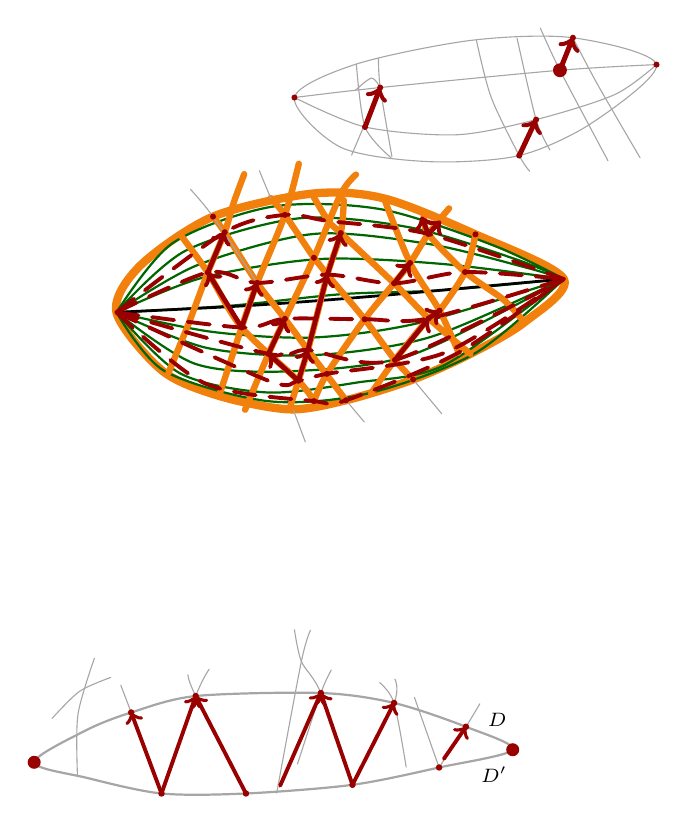
\begin{tikzpicture}[x=.55cm,y=-.55cm,line cap=round,line join=round,g/.style={olive!80!yellow,line width=1.7pt},r/.style={orange!80!brown,line width=1.8pt},w/.style={red!60!black,line width=1.5pt},b/.style={blue!60!black,line width=1.4pt},p/.style={gray!70,thin},k/.style={black,line width=1.2pt},every node/.style={font=\scriptsize}]
% Upper pencil lens with three directed short segments.
\draw[p] plot[smooth cycle] coordinates {(8.22,3.74) (9.64,2.97) (12.3,2.42) (14.65,2.36) (16.58,2.98) (15.1,4.32) (13.41,5.08) (11.31,5.22) (9.29,4.89)};
\draw[p] plot[smooth] coordinates {(8.22,3.74) (10.2,3.51) (14.35,3.11) (16.58,2.98)};
\draw[p] plot[smooth] coordinates {(8.22,3.74) (9.85,4.42) (11.97,4.6) (13.8,4.25) (15.62,3.67) (16.58,2.98)};
\draw[p] plot[smooth] coordinates {(9.65,2.98) (9.85,4.42) (10.45,5.13)};
\draw[p] plot[smooth] coordinates {(10.16,2.84) (10.2,3.51) (10.47,5.1)};
\draw[p] plot[smooth] coordinates {(9.62,3.58) (10.0,3.29) (10.2,3.51)};
\draw[p] plot[smooth] coordinates {(12.42,2.41) (12.76,3.73) (13.41,5.08) (13.65,5.44)};
\draw[p] plot[smooth] coordinates {(13.36,2.37) (13.8,4.25) (14.12,4.95)};
\draw[p] plot[smooth] coordinates {(13.9,2.14) (14.35,3.11) (15.46,5.2)};
\draw[p] plot[smooth] coordinates {(14.65,2.36) (15.22,3.44) (16.2,5.13)};
\draw[p] plot[smooth] coordinates {(9.54,5.07) (10.2,3.51)};
\draw[w,->,line width=1.8pt] plot[smooth] coordinates {(9.85,4.42) (10.2,3.51)};
\draw[w,->,line width=1.8pt] plot[smooth] coordinates {(13.41,5.08) (13.8,4.25)};
\draw[w,->,line width=1.8pt] plot[smooth] coordinates {(14.35,3.11) (14.65,2.36)};
\fill[w] (8.22,3.74) circle (.07);
\fill[w] (10.2,3.51) circle (.07);
\fill[w] (9.85,4.42) circle (.07);
\fill[w] (13.41,5.08) circle (.07);
\fill[w] (13.8,4.25) circle (.07);
\fill[w] (14.65,2.36) circle (.07);
\fill[w] (16.58,2.98) circle (.07);
\fill[w] (14.35,3.11) circle (.16);
% Large coloured lens: orange transverse curves, green longitudinal curves and dark dashed directed routes.
\draw[r,line width=3pt] plot[smooth cycle] coordinates {(4.11,8.7) (4.66,7.62) (6.34,6.49) (8.62,5.96) (10.29,6.07) (12.4,6.9) (14.44,7.93) (13.53,8.93) (12.28,9.66) (10.96,10.25) (9.41,10.73) (8.1,10.94) (6.48,10.63) (5.17,10.05)};
\draw[green!40!black,line width=.8pt] plot[smooth] coordinates {(4.11,8.7) (5.41,7.1) (7.71,6.26) (10.22,6.32) (12.83,7.16) (14.44,7.93)};
\draw[green!40!black,line width=.8pt] plot[smooth] coordinates {(4.11,8.7) (5.7,7.28) (8.32,6.53) (10.89,6.74) (13.32,7.47) (14.44,7.93)};
\draw[green!40!black,line width=.8pt] plot[smooth] coordinates {(4.11,8.7) (5.98,7.61) (8.67,6.89) (11.31,7.12) (13.58,7.67) (14.44,7.93)};
\draw[green!40!black,line width=.8pt] plot[smooth] coordinates {(4.11,8.7) (6.1,7.9) (8.8,7.47) (11.6,7.58) (14.44,7.93)};
\draw[green!40!black,line width=.8pt] plot[smooth] coordinates {(4.11,8.7) (6.71,8.55) (9.32,8.28) (11.64,8.19) (14.44,7.93)};
\draw[green!40!black,line width=.8pt] plot[smooth] coordinates {(4.11,8.7) (6.31,9.15) (8.67,9.28) (11.12,8.94) (14.44,7.93)};
\draw[green!40!black,line width=.8pt] plot[smooth] coordinates {(4.11,8.7) (6.19,9.52) (8.63,9.69) (11.36,9.27) (14.44,7.93)};
\draw[green!40!black,line width=.8pt] plot[smooth] coordinates {(4.11,8.7) (5.93,9.89) (8.14,10.06) (10.96,9.67) (14.44,7.93)};
\draw[green!40!black,line width=.8pt] plot[smooth] coordinates {(4.11,8.7) (5.58,10.11) (7.59,10.55) (9.67,10.32) (11.7,9.91) (14.44,7.93)};
\draw[green!40!black,line width=.8pt] plot[smooth] coordinates {(4.11,8.7) (5.21,10.05) (7.6,10.75) (9.89,10.58) (12.4,9.64) (14.44,7.93)};
\draw[k,line width=1pt] plot[smooth] coordinates {(4.11,8.7) (7.22,8.54) (10.14,8.32) (14.44,7.93)};
\draw[r,line width=2.3pt] plot[smooth] coordinates {(5.58,6.9) (6.22,7.78) (7.0,9.05) (8.31,10.28) (8.67,10.75)};
\draw[r,line width=2.3pt] plot[smooth] coordinates {(6.34,6.49) (6.61,6.85) (7.36,8.02) (8.0,8.85) (8.53,9.57) (9.41,10.73)};
\draw[r,line width=2.3pt] plot[smooth] coordinates {(7.67,6.06) (8.0,6.45) (8.67,7.44) (8.98,7.83) (9.84,8.86) (10.54,9.8) (10.96,10.25)};
\draw[r,line width=2.3pt] plot[smooth] coordinates {(8.62,5.96) (9.0,6.59) (9.29,6.87) (10.52,8.03) (11.32,8.84) (12.28,9.66)};
\draw[r,line width=2.3pt] plot[smooth] coordinates {(10.29,6.07) (10.89,7.56) (11.57,8.66) (12.01,9.63)};
\draw[r,line width=2.3pt] plot[smooth] coordinates {(11.21,6.44) (11.31,6.89) (12.16,7.77) (13.05,8.41) (13.53,8.93)};
\draw[r,line width=2.3pt] plot[smooth] coordinates {(5.31,10.1) (5.78,8.95) (6.22,7.78) (6.61,6.85) (6.82,6.16) (7.06,5.51)};
\draw[r,line width=2.3pt] plot[smooth] coordinates {(6.48,10.63) (7.0,9.05) (7.36,8.02) (8.0,6.45) (8.32,5.27)};
\draw[r,line width=2.3pt] plot[smooth] coordinates {(7.08,10.95) (7.62,9.66) (8.0,8.85) (8.67,7.44) (9.29,5.97) (9.64,5.52)};
\draw[r,line width=2.3pt] plot[smooth] coordinates {(8.1,10.94) (8.53,9.57) (8.98,7.83) (9.29,6.87) (9.36,6.11)};
\draw[r,line width=2.3pt] plot[smooth] coordinates {(8.67,10.75) (8.97,10.12) (9.84,8.86) (10.52,8.03) (10.89,7.56) (11.31,6.89) (11.79,6.3)};
\draw[r,line width=2.3pt] plot[smooth] coordinates {(9.99,10.57) (10.54,9.8) (11.32,8.84) (11.57,8.66) (12.16,7.77) (12.4,6.9)};
\draw[p] plot[smooth] coordinates {(5.82,5.86) (6.34,6.49) (7.36,8.02)};
\draw[p] plot[smooth] coordinates {(7.41,5.43) (7.67,6.06)};
\draw[p] plot[smooth] coordinates {(8.2,10.97) (8.47,11.69)};
\draw[p] plot[smooth] coordinates {(9.41,10.73) (9.83,11.23)};
\draw[p] plot[smooth] coordinates {(10.96,10.25) (11.62,11.04)};
\draw[w,dash pattern=on 8pt off 5pt,line width=1.4pt] plot[smooth] coordinates {(4.11,8.7) (6.61,6.85) (8.0,6.45) (9.0,6.59) (11.31,6.89) (14.44,7.93)};
\draw[w,dash pattern=on 8pt off 5pt,line width=1.4pt] plot[smooth] coordinates {(4.11,8.7) (6.22,7.78) (7.36,8.02) (8.98,7.83) (10.52,8.03) (12.16,7.77) (14.44,7.93)};
\draw[w,dash pattern=on 8pt off 5pt,line width=1.4pt] plot[smooth] coordinates {(4.11,8.7) (7.0,9.05) (8.0,8.85) (9.84,8.86) (11.32,8.84) (14.44,7.93)};
\draw[w,dash pattern=on 8pt off 5pt,line width=1.4pt] plot[smooth] coordinates {(4.11,8.7) (7.62,9.66) (8.53,9.57) (10.54,9.8) (14.44,7.93)};
\draw[w,dash pattern=on 8pt off 5pt,line width=1.4pt] plot[smooth] coordinates {(4.11,8.7) (7.62,10.28) (8.31,10.28) (8.97,10.12) (11.7,9.63) (14.44,7.93)};
\draw[w,dash pattern=on 8pt off 5pt,line width=1.4pt] plot[smooth] coordinates {(4.11,8.7) (6.15,10.34) (8.67,10.75) (9.41,10.73) (12.01,9.63) (14.44,7.93)};
\draw[w,->,line width=1.7pt] plot[smooth] coordinates {(6.22,7.78) (6.61,6.85)};
\draw[w,->,line width=1.7pt] plot[smooth] coordinates {(7.0,9.05) (6.22,7.78)};
\draw[w,->,line width=1.7pt] plot[smooth] coordinates {(7.0,9.05) (7.36,8.02)};
\draw[w,->,line width=1.7pt] plot[smooth] coordinates {(7.62,9.66) (8.0,8.85)};
\draw[w,->,line width=1.7pt] plot[smooth] coordinates {(8.31,10.28) (7.62,9.66)};
\draw[w,->,line width=1.7pt] plot[smooth] coordinates {(8.31,10.28) (8.53,9.57)};
\draw[w,->,line width=1.7pt] plot[smooth] coordinates {(8.53,9.57) (8.98,7.83)};
\draw[w,->,line width=1.7pt] plot[smooth] coordinates {(8.98,7.83) (9.29,6.87)};
\draw[w,->,line width=1.7pt] plot[smooth] coordinates {(10.52,8.03) (10.89,7.56)};
\draw[w,->,line width=1.7pt] plot[smooth] coordinates {(11.32,8.84) (11.57,8.66)};
\draw[w,->,line width=1.7pt] plot[smooth] coordinates {(10.54,9.8) (11.32,8.84)};
\draw[w,->,line width=1.7pt] plot[smooth] coordinates {(11.31,6.89) (11.6,6.59)};
\draw[w,->,line width=1.7pt] plot[smooth] coordinates {(11.31,6.89) (11.15,6.49)};
\fill[w] (6.34,6.49) circle (.07);
\fill[w] (6.61,6.85) circle (.07);
\fill[w] (6.22,7.78) circle (.07);
\fill[w] (7.0,9.05) circle (.07);
\fill[w] (7.36,8.02) circle (.07);
\fill[w] (8.0,6.45) circle (.07);
\fill[w] (8.67,7.44) circle (.07);
\fill[w] (8.98,7.83) circle (.07);
\fill[w] (9.29,6.87) circle (.07);
\fill[w] (8.0,8.85) circle (.07);
\fill[w] (7.62,9.66) circle (.07);
\fill[w] (8.53,9.57) circle (.07);
\fill[w] (8.31,10.28) circle (.07);
\fill[w] (8.67,10.75) circle (.07);
\fill[w] (8.97,10.12) circle (.07);
\fill[w] (9.41,10.73) circle (.07);
\fill[w] (9.84,8.86) circle (.07);
\fill[w] (10.52,8.03) circle (.07);
\fill[w] (10.54,9.8) circle (.07);
\fill[w] (10.96,10.25) circle (.07);
\fill[w] (10.89,7.56) circle (.07);
\fill[w] (11.31,6.89) circle (.07);
\fill[w] (11.57,8.66) circle (.07);
\fill[w] (11.32,8.84) circle (.07);
\fill[w] (12.16,7.77) circle (.07);
\fill[w] (12.4,6.9) circle (.07);
% Lower lens bounded by D and D-prime, with zigzag inward-to-upper-rim arrows.
\draw[p,line width=.8pt] plot[smooth cycle] coordinates {(2.21,19.09) (3.41,18.35) (4.45,17.94) (5.94,17.56) (8.83,17.49) (10.52,17.72) (12.18,18.27) (13.26,18.8) (11.56,19.21) (9.56,19.61) (7.1,19.81) (5.15,19.81) (3.43,19.45)};
\draw[p] plot[smooth] coordinates {(3.6,16.69) (3.22,17.99) (3.21,19.4)};
\draw[p] plot[smooth] coordinates {(4.21,17.31) (4.45,17.94) (5.15,19.81)};
\draw[p] plot[smooth] coordinates {(6.25,16.94) (5.94,17.56) (5.15,19.81)};
\draw[p] plot[smooth] coordinates {(5.76,17.07) (5.94,17.56) (7.1,19.81)};
\draw[p] plot[smooth] coordinates {(8.22,16.03) (8.38,16.76) (8.83,17.49) (9.56,19.61)};
\draw[p] plot[smooth] coordinates {(8.59,16.04) (8.38,16.76) (7.81,19.8)};
\draw[p] plot[smooth] coordinates {(9.07,16.96) (8.83,17.49) (8.29,19.13)};
\draw[p] plot[smooth] coordinates {(10.54,17.17) (10.52,17.72) (9.56,19.61)};
\draw[p] plot[smooth] coordinates {(10.19,17.25) (10.52,17.72) (10.8,19.2)};
\draw[p] plot[smooth] coordinates {(10.99,17.59) (11.56,19.21)};
\draw[p] plot[smooth] coordinates {(12.5,17.74) (12.18,18.27) (11.56,19.21)};
\draw[p] plot[smooth] coordinates {(2.62,18.08) (3.26,17.45) (3.98,17.13)};
\draw[w,->,line width=1.4pt] plot[smooth] coordinates {(5.15,19.81) (4.45,17.94)};
\draw[w,->,line width=1.4pt] plot[smooth] coordinates {(5.15,19.81) (5.94,17.56)};
\draw[w,->,line width=1.4pt] plot[smooth] coordinates {(7.1,19.81) (5.94,17.56)};
\draw[w,->,line width=1.4pt] plot[smooth] coordinates {(7.89,19.63) (8.83,17.49)};
\draw[w,->,line width=1.4pt] plot[smooth] coordinates {(9.56,19.61) (8.83,17.49)};
\draw[w,->,line width=1.4pt] plot[smooth] coordinates {(9.56,19.61) (10.52,17.72)};
\draw[w,->,line width=1.4pt] plot[smooth] coordinates {(11.67,19.01) (12.18,18.27)};
\fill[w] (2.21,19.09) circle (.15);
\fill[w] (13.26,18.8) circle (.15);
\fill[w] (4.45,17.94) circle (.075);
\fill[w] (5.94,17.56) circle (.075);
\fill[w] (8.83,17.49) circle (.075);
\fill[w] (10.52,17.72) circle (.075);
\fill[w] (12.18,18.27) circle (.075);
\fill[w] (11.56,19.21) circle (.075);
\fill[w] (9.56,19.61) circle (.075);
\fill[w] (7.1,19.81) circle (.075);
\fill[w] (5.15,19.81) circle (.075);
\node at (12.9,18.1) {$D$};
\node at (12.83,19.37) {$D'$};
\end{tikzpicture}}

\margin{\uline{NB} Même une fois complété par les \unsure{fuseaux} adjacents, le couple \unsure{de flèches} \unsure{demeure} \illegible{1}\ \unsure{disconnexe} (car il y a une comp. connexe \unsure{libre}\ -- \unsure{bord du fuseau}).}

\unsure{types} de fuseaux :

1) couloirs : les deux rives sont \unsure{supracritiques} \inserted{(ou fuseaux \deleted{\unsure{biparalléliques}})}

\unsure{3|2}) semi-couloirs : un (et un seul) des deux rives est \unsure{supracritique}.
\inserted{(fuseaux \deleted{\unsure{paralléliques}} \unsure{unilatéraux})}
\inserted{\unsure{triviaux}}

3) fuseaux \uline{ordinaires}

\deleted{ordinaire}
Fuseau : comp. connexe $C$ déterminée par deux ps. droites $D,D'$ en $\unsure{X}$ (qui peuvent être $\unsure{\in}\Sigma$) \deleted{\unsure{telles}} que

\begin{align*}
\text{a)}\quad&\Sigma\cup\{D,D'\}=\Sigma'\quad\inserted{\text{\unsure{syst.} de ps. dr.}}\\
\text{b)}\quad& D\ne D',\ \unsure{\Rightarrow}\ \text{et }\unsure{\{s,\bar s\}}=D\cap D'
\end{align*}
\unsure{sont des sommets de} $\Sigma$

c) $C$ est un couloir de $\unsure{\Sigma'_{\sigma\ne1}}$

\unsure{d}) $D$ et $D'$ sont critiques pour $\Sigma$.

Chaque fuseau détermine une p.r. semi-stble, et on a une corresp. $1-1$ entre \inserted{(classes d'isotopie de)} fuseaux et p.r. semi-stbles. \inserted{\uline{canon.}}

\unsure{d}) signifie aussi que tt \deleted{\unsure{triangle}} \inserted{\unsure{triangle}} de contraction sur la \uline{rive libre} de $D$ ou $D'$ est accolé à un sommet, et qu'à l'intérieur du fuseau, chaque sommet sur une rive est relié à un sommet sur l'autre \inserted{(cas \unsure{I} de type I ou II)}.
Sauf dans cas triviaux, un fuseau est déterminé par les (classes d'isotopie) de ses rives.
\margin{\mspage{152}}

\scanpage{154}
{\ttfamily\unsure{//CRAY2} JOB '*********',\\
// MSGLEVEL=(1,1),MSGCLASS=A\\
// EXEC PGM=IEFBR14\qquad JOB 0025}
\figure{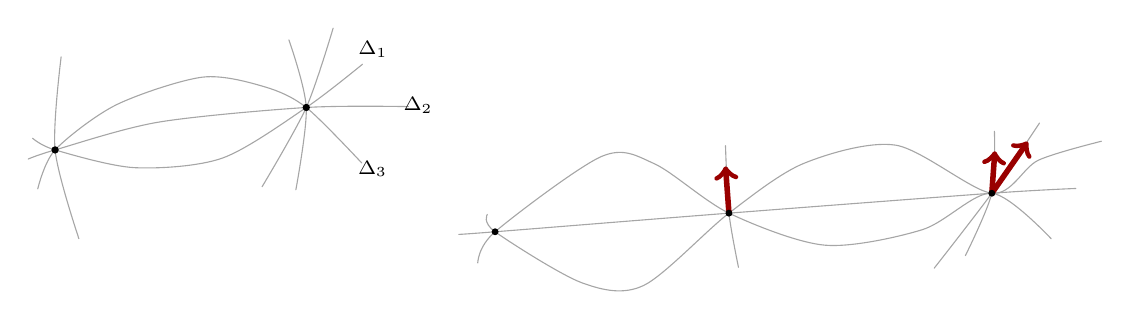
\begin{tikzpicture}[x=.55cm,y=-.55cm,line cap=round,line join=round,g/.style={olive!80!yellow,line width=1.7pt},r/.style={orange!80!brown,line width=1.8pt},w/.style={red!60!black,line width=1.5pt},b/.style={blue!60!black,line width=1.4pt},p/.style={gray!70,thin},k/.style={black,line width=1.2pt},every node/.style={font=\scriptsize}]
\draw[p] plot[smooth] coordinates {(2.7,3.96) (3.32,3.75) (5.7,3.11) (9.12,2.77) (11.48,2.75)};
\draw[p] plot[smooth] coordinates {(2.92,4.65) (3.32,3.75) (4.73,2.71) (6.72,2.07) (8.15,2.29) (9.12,2.77) (10.4,4.05)};
\draw[p] plot[smooth] coordinates {(2.8,3.48) (3.32,3.75) (5.16,4.16) (7.18,3.94) (9.12,2.77) (10.42,1.77)};
\draw[p] plot[smooth] coordinates {(3.46,1.6) (3.32,3.75) (3.87,5.8)};
\draw[p] plot[smooth] coordinates {(8.72,1.21) (9.12,2.77) (8.88,4.67)};
\draw[p] plot[smooth] coordinates {(9.74,.94) (9.12,2.77) (8.1,4.6)};
\fill[k] (3.32,3.75) circle (.085);
\fill[k] (9.12,2.77) circle (.085);
\node at (10.66,1.43) {$\Delta_1$};
\node at (11.7,2.72) {$\Delta_2$};
\node at (10.65,4.19) {$\Delta_3$};
\draw[p] plot[smooth] coordinates {(12.64,5.7) (13.48,5.64) (18.88,5.21) (24.95,4.75) (26.89,4.64)};
\draw[p] plot[smooth] coordinates {(13.08,6.36) (13.48,5.64) (15.94,3.9) (17.16,4.07) (18.88,5.21) (21.1,5.95) (23.35,5.59) (24.95,4.75) (26.32,5.8)};
\draw[p] plot[smooth] coordinates {(13.3,5.24) (13.48,5.64) (15.49,6.82) (16.91,6.88) (18.88,5.21) (20.61,4.06) (22.73,3.64) (24.95,4.75) (26.02,3.99) (27.48,3.55)};
\draw[p] plot[smooth] coordinates {(18.8,3.65) (18.88,5.21) (19.1,6.46)};
\draw[p] plot[smooth] coordinates {(25.01,3.32) (24.95,4.75) (24.34,6.19)};
\draw[p] plot[smooth] coordinates {(26.05,3.13) (24.95,4.75) (23.62,6.48)};
\draw[w,->,line width=2pt] plot[smooth] coordinates {(18.88,5.21) (18.8,4.13)};
\draw[w,->,line width=2pt] plot[smooth] coordinates {(24.95,4.75) (25.02,3.78)};
\draw[w,->,line width=2pt] plot[smooth] coordinates {(24.95,4.75) (25.78,3.56)};
\fill[k] (13.48,5.64) circle (.08);
\fill[k] (18.88,5.21) circle (.08);
\fill[k] (24.95,4.75) circle (.08);
\end{tikzpicture}}

Soit $D$ position relative non principale,
$S_D$ \inserted{$=D\cap S$} \unsure{l'ens.} des sommets multiples de $D$ $(\operatorname{card}S_D\geq2)$.

1) Toute position relative \uline{principale} \inserted{(donc critique)} qui passe par $S_D$ est-elle une spécialisation de $D$ ?

Pour celles \inserted{$\unsure{D'}=\unsure{D'_\delta}$} qui sont des spécialisations de $D$ (\uline{NB} elles ne sont \uline{pas} supracritiques), à chacune d'elle est associé un système de flèches d'orientation des $\Delta_s$ $(s\in S_{\unsure{D'}}\setminus S_D)$ qui ``\unsure{pointent}'' vers $\delta$, et un sens pour parcourir les $\Delta_\sigma$ $(\sigma\in S_D)$.
Pour un $\delta$ donné, ce système de flèches détermine \unsure{déjà} $D$.
\[
\prod_{s\in S_{D'}\setminus S_D}\varepsilon_{\deleted{\unsure{\delta}}D',s}
\qquad \deleted{\unsure{s}}
\]
Il y a aussi le système des \deleted{\unsure{flèches}} \inserted{p.r. stbles} qui générisent $D$,

Les générisations stbles de $D$ correspondent aux sommets d'un cube \unsure{canon.} de dim $\nu$, dont les \unsure{arêtes} sont les générisations semi-stbles, et la relation d'incidence entre sommets et arêtes est la relation de spécialisation.
\figure{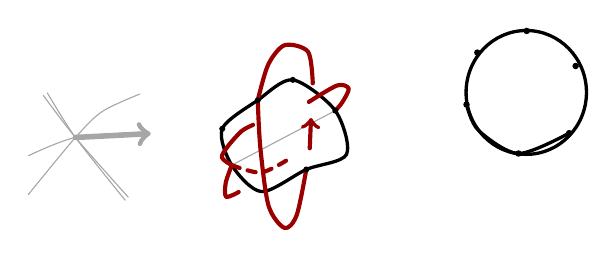
\begin{tikzpicture}[x=.55cm,y=-.55cm,line cap=round,line join=round,g/.style={olive!80!yellow,line width=1.7pt},r/.style={orange!80!brown,line width=1.8pt},w/.style={red!60!black,line width=1.5pt},b/.style={blue!60!black,line width=1.4pt},p/.style={gray!70,thin},k/.style={black,line width=1.2pt},every node/.style={font=\scriptsize}]
\draw[p] plot[smooth] coordinates {(8.86,19.4) (9.94,18.98) (11.5,18.86)};
\draw[p] plot[smooth] coordinates {(8.85,20.3) (9.94,18.98) (10.56,18.38) (11.42,17.98)};
\draw[p] plot[smooth] coordinates {(9.29,17.95) (9.94,18.98) (11.09,20.43)};
\draw[p] plot[smooth] coordinates {(9.2,18.01) (9.94,18.98) (11.16,20.36)};
\draw[p,->,line width=2pt] plot[smooth] coordinates {(9.94,18.98) (11.68,18.89)};
\draw[k] plot[smooth cycle] coordinates {(13.33,18.78) (14.15,18.12) (14.96,17.65) (15.94,18.36) (16.2,19.37) (15.27,19.72) (14.24,20.23) (13.55,19.62)};
\draw[p] plot[smooth] coordinates {(13.55,19.62) (15.94,18.36)};
\draw[w] plot[smooth] coordinates {(14.15,18.12) (14.39,17.3) (14.77,16.85) (15.31,17.0) (15.42,17.73)};
\draw[w] plot[smooth] coordinates {(15.33,18.16) (15.98,17.78) (16.25,17.85) (16.1,18.17) (15.94,18.36)};
\draw[w] plot[smooth] coordinates {(14.15,18.12) (14.21,19.22) (14.4,20.56) (14.77,21.07) (15.05,20.77) (15.27,19.72)};
\draw[w] plot[smooth] coordinates {(13.55,19.62) (13.32,19.44) (13.47,19.17) (13.78,18.83) (14.04,18.69)};
\draw[w] plot[smooth] coordinates {(13.55,19.62) (13.41,20.03) (13.42,20.35) (13.71,20.24)};
\draw[w,dashed] plot[smooth] coordinates {(13.55,19.62) (14.22,19.79) (14.83,19.5)};
\draw[w,->] plot[smooth] coordinates {(15.35,19.23) (15.38,18.53)};
\fill[k] (13.33,18.78) circle (.07);
\fill[k] (14.15,18.12) circle (.07);
\fill[k] (14.96,17.65) circle (.07);
\fill[k] (15.94,18.36) circle (.07);
\fill[k] (15.27,19.72) circle (.07);
\draw[k] (20.35,17.94) ellipse (1.39 and 1.43);
\draw[k] plot[smooth] coordinates {(18.97,18.22) (19.24,18.81) (20.17,19.35) (21.34,18.88)};
\fill[k] (19.22,17.02) circle (.075);
\fill[k] (20.36,16.52) circle (.075);
\fill[k] (21.49,17.33) circle (.075);
\fill[k] (21.34,18.88) circle (.075);
\fill[k] (20.17,19.35) circle (.075);
\fill[k] (18.97,18.22) circle (.075);
\end{tikzpicture}}

\unsure{Produit} des diagonales d'un polygone \inserted{\unsure{convexe}} \unsure{régulier}
\deleted{degré} $2\nu$.
\[
2^{\nu\unsure{+}}\ \text{sommets},\quad \nu2^{\nu-1}\ \text{arêtes}
\]
\margin{\mspage{153}}

\scanpage{155}
{\ttfamily
* \unsure{LE NIVEAU DU SYSTEME} MVS/SP \unsure{1.3|1.1} SERA MIS EN SERVICE SUR LE *\\
* 3081 LE 21 AOUT 1982. *\\
*\hfill *\\
******************************************************************}
\figure{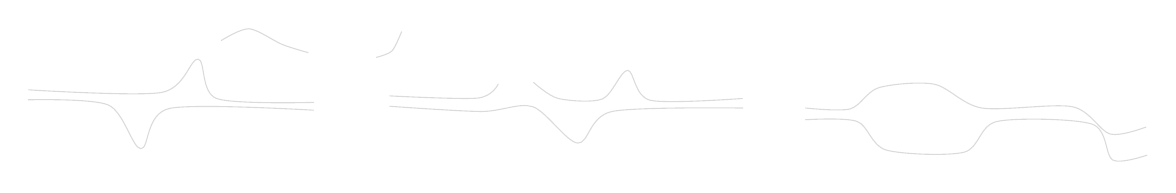
\begin{tikzpicture}[x=.55cm,y=-.55cm,line cap=round,line join=round,g/.style={olive!80!yellow,line width=1.7pt},r/.style={orange!80!brown,line width=1.8pt},w/.style={red!60!black,line width=1.5pt},b/.style={blue!60!black,line width=1.4pt},p/.style={gray!70,thin},k/.style={black,line width=1.2pt},every node/.style={font=\scriptsize}]
\draw[p,opacity=.4] plot[smooth] coordinates {(1.8,2.97) (4.87,3.03) (5.71,2.26) (6.14,3.17) (8.38,3.26)};
\draw[p,opacity=.4] plot[smooth] coordinates {(1.79,3.2) (3.64,3.32) (4.39,4.33) (5.05,3.4) (8.38,3.44)};
\draw[p,opacity=.4] plot[smooth] coordinates {(6.25,1.83) (6.89,1.56) (7.65,1.92) (8.25,2.11)};
\draw[p,opacity=.4] plot[smooth] coordinates {(9.83,2.22) (10.19,2.07) (10.41,1.63)};
\draw[p,opacity=.4] plot[smooth] coordinates {(10.14,3.11) (12.17,3.16) (12.64,2.84)};
\draw[p,opacity=.4] plot[smooth] coordinates {(10.14,3.35) (12.25,3.47) (13.44,3.36) (14.48,4.2) (15.27,3.47) (18.29,3.39)};
\draw[p,opacity=.4] plot[smooth] coordinates {(13.46,2.8) (14.03,3.17) (15.05,3.18) (15.63,2.52) (16.15,3.21) (18.28,3.17)};
\draw[p,opacity=.4] plot[smooth] coordinates {(19.74,3.39) (20.77,3.41) (21.43,2.92) (22.71,2.84) (23.81,3.39) (25.9,3.36) (26.77,3.99) (27.6,3.83)};
\draw[p,opacity=.4] plot[smooth] coordinates {(19.74,3.66) (20.93,3.7) (21.6,4.36) (23.4,4.41) (24.16,3.7) (26.35,3.76) (26.83,4.59) (27.62,4.48)};
\end{tikzpicture}}
balayages élémentaires de positions relatives
\figure{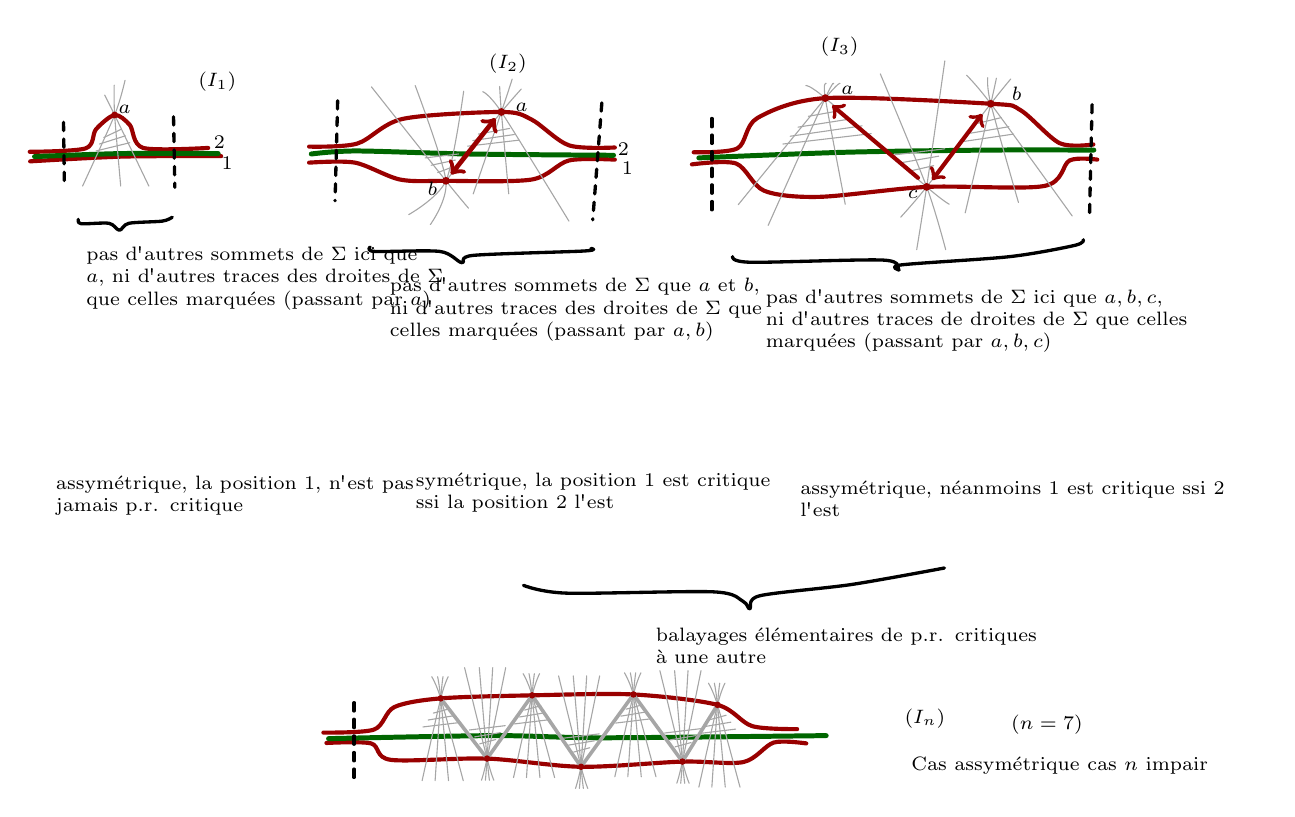
\begin{tikzpicture}[x=.55cm,y=-.55cm,line cap=round,line join=round,g/.style={olive!80!yellow,line width=1.7pt},r/.style={orange!80!brown,line width=1.8pt},w/.style={red!60!black,line width=1.5pt},b/.style={blue!60!black,line width=1.4pt},p/.style={gray!70,thin},k/.style={black,line width=1.2pt},every node/.style={font=\scriptsize}]
\draw[w] plot[smooth] coordinates {(2.87,7.0) (4.16,6.92) (4.4,6.48) (4.83,6.15) (5.18,6.38) (5.49,6.91) (6.99,6.91)};
\draw[w] plot[smooth] coordinates {(2.88,7.22) (5.02,7.11) (7.29,7.1)};
\draw[green!40!black,line width=1.8pt] plot[smooth] coordinates {(2.98,7.11) (5.0,7.04) (7.22,7.04)};
\draw[p] plot[smooth] coordinates {(4.6,5.69) (4.83,6.15) (5.62,7.79)};
\draw[p] plot[smooth] coordinates {(5.07,5.35) (4.83,6.15) (4.09,7.79)};
\draw[p] plot[smooth] coordinates {(4.82,5.46) (4.83,6.15) (4.97,7.79)};
\draw[p] plot[smooth] coordinates {(4.58,6.67) (4.98,6.48)};
\draw[p] plot[smooth] coordinates {(4.48,6.82) (5.08,6.63)};
\draw[p] plot[smooth] coordinates {(4.4,6.98) (5.18,6.79)};
\draw[k,dashed] plot[smooth] coordinates {(3.65,6.32) (3.67,7.75)};
\draw[k,dashed] plot[smooth] coordinates {(6.19,6.19) (6.22,7.82)};
\fill[w] (4.83,6.15) circle (.08);
\node at (5.06,6.03) {$a$};
\node at (7.2,5.39) {$(I_1)$};
\node at (7.25,6.79) {$2$};
\node at (7.43,7.26) {$1$};
\draw[k] plot[smooth] coordinates {(3.99,8.56) (4.06,8.66) (4.7,8.65) (4.94,8.81) (5.16,8.65) (5.93,8.6) (6.16,8.51)};
\node[anchor=north west,align=left,text width=4.7cm] at (3.95,8.98) {pas d\textquotesingle autres sommets de $\Sigma$ ici que $a$, ni d\textquotesingle autres traces des droites de $\Sigma$ que \deleted{\unsure{celles}} marquées (passant par $a$)};
\node[anchor=north west,align=left,text width=4.7cm] at (3.25,14.25) {\uline{assymétrique}, la position 1, n\textquotesingle est \uline{pas} \deleted{\unsure{jamais}} p.r. critique};
\draw[w] plot[smooth] coordinates {(9.32,6.88) (10.43,6.81) (11.48,6.24) (13.76,6.08) (14.45,6.25) (15.32,6.85) (16.38,6.9)};
\draw[w] plot[smooth] coordinates {(9.32,7.25) (10.38,7.25) (11.42,7.64) (12.48,7.67) (14.46,7.64) (15.32,7.2) (16.38,7.18)};
\draw[green!40!black,line width=1.8pt] plot[smooth] coordinates {(9.37,7.05) (10.4,6.98) (13.0,7.05) (16.35,7.08)};
\draw[p] plot[smooth] coordinates {(10.76,5.5) (12.48,7.67) (13.0,8.3)};
\draw[p] plot[smooth] coordinates {(11.77,5.47) (12.48,7.67) (12.12,8.68)};
\draw[p] plot[smooth] coordinates {(12.89,5.6) (12.48,7.67) (11.62,8.45)};
\draw[p] plot[smooth] coordinates {(13.11,7.97) (13.76,6.08) (14.01,5.32)};
\draw[p] plot[smooth] coordinates {(13.33,5.61) (13.76,6.08) (15.32,8.6)};
\draw[p] plot[smooth] coordinates {(13.72,5.49) (13.76,6.08) (13.93,7.97)};
\draw[p] plot[smooth] coordinates {(14.22,5.55) (13.76,6.08) (12.48,7.67)};
\draw[p] plot[smooth] coordinates {(12.98,6.87) (14.17,6.73)};
\draw[p] plot[smooth] coordinates {(13.1,6.74) (14.06,6.6)};
\draw[p] plot[smooth] coordinates {(13.23,6.59) (13.95,6.46)};
\draw[p] plot[smooth] coordinates {(12.0,7.14) (12.77,7.05)};
\draw[p] plot[smooth] coordinates {(12.14,7.31) (12.7,7.19)};
\draw[p] plot[smooth] coordinates {(12.29,7.48) (12.58,7.37)};
\draw[w,<->,line width=1.7pt] plot[smooth] coordinates {(12.6,7.52) (13.62,6.23)};
\draw[k,dashed] plot[smooth] coordinates {(9.98,5.82) (9.92,8.13)};
\draw[k,dashed] plot[smooth] coordinates {(16.08,5.87) (15.87,8.57)};
\fill[w] (13.76,6.08) circle (.09);
\fill[w] (12.48,7.67) circle (.09);
\node at (14.23,5.98) {$a$};
\node at (12.17,7.86) {$b$};
\node at (13.91,4.96) {$(I_2)$};
\node at (16.58,6.94) {$2$};
\node at (16.67,7.39) {$1$};
\draw[k] plot[smooth] coordinates {(10.73,9.2) (10.84,9.3) (12.34,9.3) (12.85,9.56) (13.12,9.39) (15.67,9.29) (15.83,9.23)};
\node[anchor=north west,align=left,text width=4.8cm] at (10.96,9.7) {pas d\textquotesingle autres sommets de $\Sigma$ que $a$ et $b$, ni d\textquotesingle autres traces des droites de $\Sigma$ que celles marquées (passant par $a,b$)};
\node[anchor=north west,align=left,text width=4.8cm] at (11.56,14.2) {\uline{symétrique}, la position 1 est critique ssi la position 2 l\textquotesingle est};
\draw[w] plot[smooth] coordinates {(18.2,7.01) (19.21,6.92) (19.67,6.22) (21.24,5.76) (25.06,5.89) (25.75,6.04) (26.65,6.8) (27.43,6.83)};
\draw[w] plot[smooth] coordinates {(18.16,7.29) (19.18,7.27) (19.83,7.9) (21.1,8.04) (23.58,7.81) (26.29,7.79) (26.88,7.2) (27.52,7.18)};
\draw[green!40!black,line width=1.8pt] plot[smooth] coordinates {(18.32,7.14) (21.7,7.01) (25.0,6.96) (27.44,6.96)};
\draw[p] plot[smooth] coordinates {(20.79,5.47) (21.24,5.76) (23.58,7.81) (24.1,8.21)};
\draw[p] plot[smooth] coordinates {(21.58,5.42) (21.24,5.76) (19.23,8.22)};
\draw[p] plot[smooth] coordinates {(21.26,5.42) (21.24,5.76) (21.7,8.21)};
\draw[p] plot[smooth] coordinates {(21.43,5.43) (21.24,5.76) (19.92,8.7)};
\draw[p] plot[smooth] coordinates {(22.51,5.2) (23.58,7.81) (24.02,9.26)};
\draw[p] plot[smooth] coordinates {(24.0,4.9) (23.58,7.81) (23.35,9.26)};
\draw[p] plot[smooth] coordinates {(24.5,5.23) (25.06,5.89) (26.94,8.48)};
\draw[p] plot[smooth] coordinates {(25.19,5.3) (25.06,5.89) (24.47,8.41)};
\draw[p] plot[smooth] coordinates {(25.52,5.32) (25.06,5.89) (23.58,7.81) (22.98,8.51)};
\draw[p] plot[smooth] coordinates {(24.99,5.29) (25.06,5.89) (25.7,8.17)};
\draw[p] plot[smooth] coordinates {(20.26,6.82) (22.3,6.58)};
\draw[p] plot[smooth] coordinates {(20.43,6.64) (22.09,6.4)};
\draw[p] plot[smooth] coordinates {(20.61,6.43) (21.83,6.24)};
\draw[p] plot[smooth] coordinates {(20.85,6.18) (21.57,6.05)};
\draw[p] plot[smooth] coordinates {(22.84,7.07) (24.0,6.93)};
\draw[p] plot[smooth] coordinates {(23.0,7.25) (23.86,7.1)};
\draw[p] plot[smooth] coordinates {(23.21,7.44) (23.74,7.32)};
\draw[p] plot[smooth] coordinates {(24.44,6.76) (25.59,6.59)};
\draw[p] plot[smooth] coordinates {(24.59,6.57) (25.48,6.42)};
\draw[p] plot[smooth] coordinates {(24.77,6.34) (25.3,6.21)};
\draw[w,->] plot[smooth] coordinates {(23.38,7.6) (21.4,5.93)};
\draw[w,<->] plot[smooth] coordinates {(23.71,7.65) (24.86,6.13)};
\draw[k,dashed] plot[smooth] coordinates {(18.62,6.23) (18.62,8.43)};
\draw[k,dashed] plot[smooth] coordinates {(27.4,5.91) (27.34,8.5)};
\fill[w] (21.24,5.76) circle (.09);
\fill[w] (25.06,5.89) circle (.09);
\fill[w] (23.58,7.81) circle (.09);
\node at (21.75,5.58) {$a$};
\node at (25.66,5.66) {$b$};
\node at (23.26,7.98) {$c$};
\node at (21.57,4.57) {$(I_3)$};
\draw[k] plot[smooth] coordinates {(19.1,9.42) (19.52,9.55) (22.58,9.5) (22.94,9.73) (23.0,9.61) (25.5,9.42) (27.0,9.16) (27.2,9.03)};
\node[anchor=north west,align=left,text width=5.9cm] at (19.64,9.97) {pas d\textquotesingle autres sommets de $\Sigma$ ici que $a,b,c$, ni d\textquotesingle autres traces de droites de $\Sigma$ que celles marquées (passant par $a,b,c$)};
\node[anchor=north west,align=left,text width=5.8cm] at (20.44,14.37) {\uline{assymétrique}, néanmoins 1 est critique ssi 2 l\textquotesingle est};
\draw[k] plot[smooth] coordinates {(14.27,17.01) (15.26,17.19) (18.65,17.16) (19.34,17.38) (19.5,17.55) (19.73,17.25) (21.85,16.99) (23.99,16.61)};
\node[anchor=north west,align=left,text width=5cm] at (17.1,17.76) {balayages élémentaires de p.r. critiques \unsure{à une} \unsure{autre}};
\draw[w] plot[smooth] coordinates {(9.65,20.41) (10.82,20.34) (11.29,19.82) (12.36,19.62) (14.47,19.55) (16.81,19.53) (18.75,19.77) (19.55,20.26) (20.59,20.33)};
\draw[w] plot[smooth] coordinates {(9.72,20.65) (10.75,20.66) (11.21,21.04) (13.43,21.01) (15.6,21.2) (17.94,21.08) (19.35,21.09) (20.05,20.64) (20.8,20.66)};
\draw[green!40!black,line width=1.8pt] plot[smooth] coordinates {(9.77,20.55) (13.59,20.48) (16.1,20.53) (21.26,20.48)};
\draw[k,dashed] plot[smooth] coordinates {(10.36,19.72) (10.36,21.55)};
\draw[p,line width=1.3pt] (12.36,19.62)--(13.43,21.01)--(14.47,19.55)--(15.6,21.2)--(16.81,19.53)--(17.94,21.08)--(18.75,19.77);
\draw[p] plot[smooth] coordinates {(12.532,19.12) (12.36,19.62) (11.93,21.52)};
\draw[p] plot[smooth] coordinates {(12.411999999999999,19.12) (12.36,19.62) (12.229999999999999,21.52)};
\draw[p] plot[smooth] coordinates {(12.288,19.12) (12.36,19.62) (12.54,21.52)};
\draw[p] plot[smooth] coordinates {(12.152,19.12) (12.36,19.62) (12.879999999999999,21.52)};
\draw[p] (12.19,19.96)--(12.559999999999999,19.86);
\draw[p] (12.07,20.12)--(12.669999999999998,20.02);
\draw[p] (11.95,20.28)--(12.78,20.18);
\draw[p] plot[smooth] coordinates {(13.86,18.91) (13.43,21.01) (13.301,21.51)};
\draw[p] plot[smooth] coordinates {(13.56,18.91) (13.43,21.01) (13.391,21.51)};
\draw[p] plot[smooth] coordinates {(13.25,18.91) (13.43,21.01) (13.484,21.51)};
\draw[p] plot[smooth] coordinates {(12.91,18.91) (13.43,21.01) (13.586,21.51)};
\draw[p] (13.26,20.67)--(13.629999999999999,20.57);
\draw[p] (13.14,20.51)--(13.739999999999998,20.41);
\draw[p] (13.02,20.35)--(13.85,20.25);
\draw[p] plot[smooth] coordinates {(14.642000000000001,19.05) (14.47,19.55) (14.040000000000001,21.45)};
\draw[p] plot[smooth] coordinates {(14.522,19.05) (14.47,19.55) (14.34,21.45)};
\draw[p] plot[smooth] coordinates {(14.398000000000001,19.05) (14.47,19.55) (14.65,21.45)};
\draw[p] plot[smooth] coordinates {(14.262,19.05) (14.47,19.55) (14.99,21.45)};
\draw[p] (14.3,19.89)--(14.67,19.79);
\draw[p] (14.180000000000001,20.05)--(14.78,19.95);
\draw[p] (14.06,20.21)--(14.89,20.11);
\draw[p] plot[smooth] coordinates {(16.03,19.099999999999998) (15.6,21.2) (15.471,21.7)};
\draw[p] plot[smooth] coordinates {(15.73,19.099999999999998) (15.6,21.2) (15.561,21.7)};
\draw[p] plot[smooth] coordinates {(15.42,19.099999999999998) (15.6,21.2) (15.654,21.7)};
\draw[p] plot[smooth] coordinates {(15.08,19.099999999999998) (15.6,21.2) (15.756,21.7)};
\draw[p] (15.43,20.86)--(15.799999999999999,20.759999999999998);
\draw[p] (15.31,20.7)--(15.909999999999998,20.599999999999998);
\draw[p] (15.19,20.54)--(16.02,20.439999999999998);
\draw[p] plot[smooth] coordinates {(16.982,19.03) (16.81,19.53) (16.38,21.43)};
\draw[p] plot[smooth] coordinates {(16.862,19.03) (16.81,19.53) (16.68,21.43)};
\draw[p] plot[smooth] coordinates {(16.738,19.03) (16.81,19.53) (16.99,21.43)};
\draw[p] plot[smooth] coordinates {(16.602,19.03) (16.81,19.53) (17.33,21.43)};
\draw[p] (16.639999999999997,19.87)--(17.009999999999998,19.77);
\draw[p] (16.519999999999996,20.03)--(17.119999999999997,19.93);
\draw[p] (16.4,20.19)--(17.229999999999997,20.09);
\draw[p] plot[smooth] coordinates {(18.37,18.979999999999997) (17.94,21.08) (17.811,21.58)};
\draw[p] plot[smooth] coordinates {(18.07,18.979999999999997) (17.94,21.08) (17.901,21.58)};
\draw[p] plot[smooth] coordinates {(17.76,18.979999999999997) (17.94,21.08) (17.994,21.58)};
\draw[p] plot[smooth] coordinates {(17.42,18.979999999999997) (17.94,21.08) (18.096,21.58)};
\draw[p] (17.77,20.74)--(18.14,20.639999999999997);
\draw[p] (17.65,20.58)--(18.25,20.479999999999997);
\draw[p] (17.53,20.419999999999998)--(18.36,20.319999999999997);
\draw[p] plot[smooth] coordinates {(18.922,19.27) (18.75,19.77) (18.32,21.669999999999998)};
\draw[p] plot[smooth] coordinates {(18.802,19.27) (18.75,19.77) (18.62,21.669999999999998)};
\draw[p] plot[smooth] coordinates {(18.678,19.27) (18.75,19.77) (18.93,21.669999999999998)};
\draw[p] plot[smooth] coordinates {(18.542,19.27) (18.75,19.77) (19.27,21.669999999999998)};
\draw[p] (18.58,20.11)--(18.95,20.009999999999998);
\draw[p] (18.459999999999997,20.27)--(19.06,20.169999999999998);
\draw[p] (18.34,20.43)--(19.169999999999998,20.33);
\fill[w] (12.36,19.62) circle (.075);
\fill[w] (13.43,21.01) circle (.075);
\fill[w] (14.47,19.55) circle (.075);
\fill[w] (15.6,21.2) circle (.075);
\fill[w] (16.81,19.53) circle (.075);
\fill[w] (17.94,21.08) circle (.075);
\fill[w] (18.75,19.77) circle (.075);
\node at (23.54,20.08) {$(I_n)$};
\node at (26.36,20.23) {$(n=7)$};
\node[anchor=west] at (23.0,21.18) {Cas \unsure{assymétrique} cas $n$ impair};
\end{tikzpicture}}
\margin{\mspage{154}}

\scanpage{156}
\figure{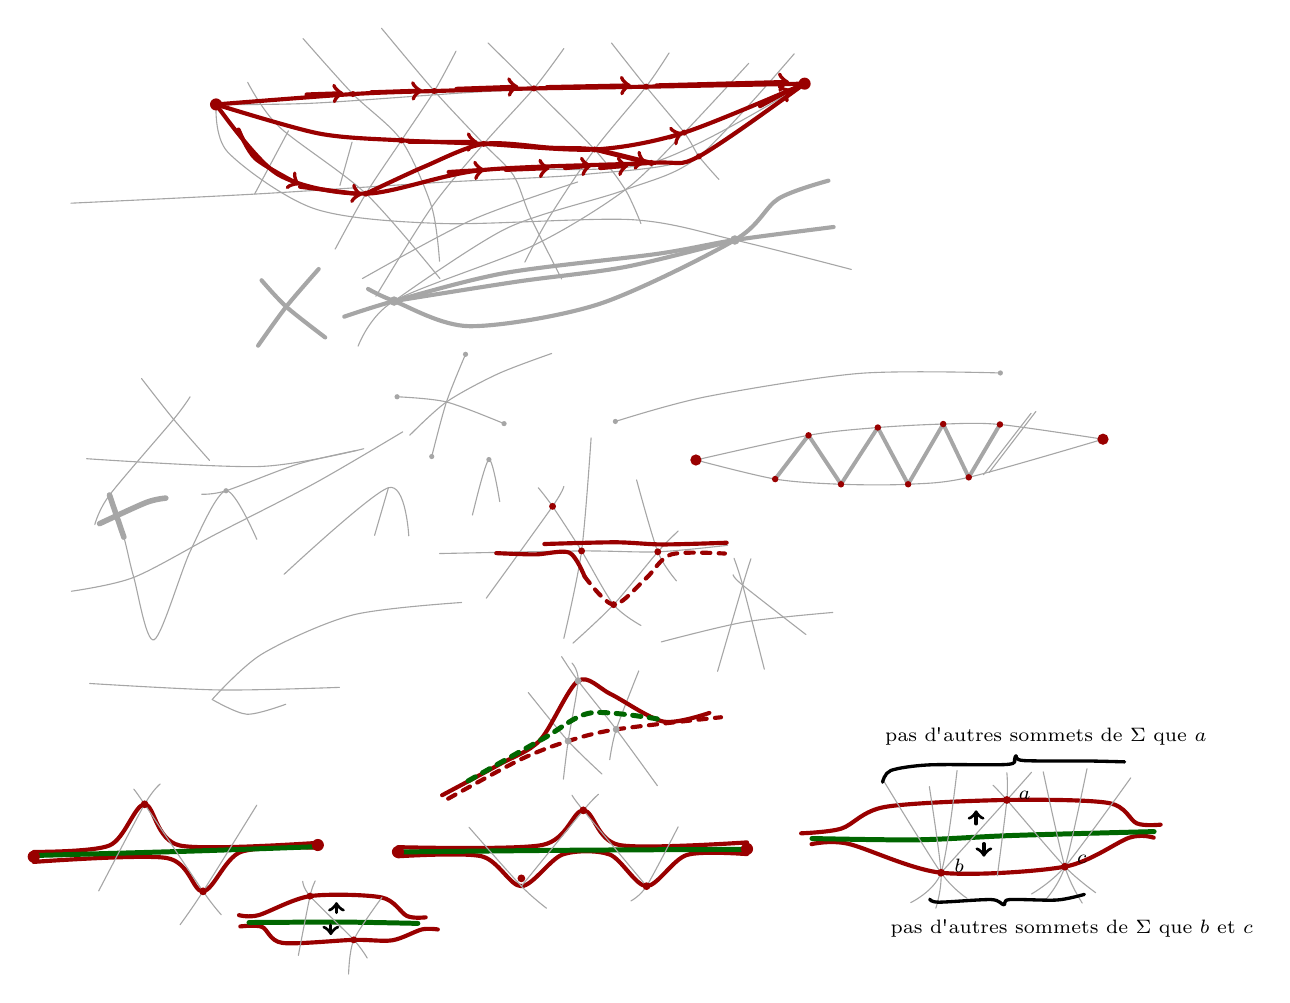
\begin{tikzpicture}[x=.55cm,y=-.55cm,line cap=round,line join=round,g/.style={olive!80!yellow,line width=1.7pt},r/.style={orange!80!brown,line width=1.8pt},w/.style={red!60!black,line width=1.5pt},b/.style={blue!60!black,line width=1.4pt},p/.style={gray!70,thin},k/.style={black,line width=1.2pt},every node/.style={font=\scriptsize}]
\draw[p] plot[smooth] coordinates {(6.04,1.92) (6.31,3.02) (8.32,4.33) (11.27,4.67) (15.63,4.58) (18.02,5.05) (20.71,5.73)};
\draw[p] plot[smooth] coordinates {(6.04,1.92) (8.3,1.89) (12.47,1.61) (16.12,1.51) (19.63,1.44)};
\draw[p] plot[smooth] coordinates {(6.04,1.92) (8.41,2.59) (10.32,2.75) (12.22,2.83) (14.78,2.96) (16.85,2.57) (19.63,1.44)};
\draw[p] plot[smooth] coordinates {(6.04,1.92) (7.46,3.53) (9.5,3.98) (12.14,3.44) (16.09,3.27) (19.63,1.44)};
\draw[p] plot[smooth] coordinates {(2.69,4.2) (6.93,3.99) (11.2,3.72) (14.61,3.53) (17.19,3.12) (19.63,1.44)};
\draw[p] plot[smooth] coordinates {(6.77,1.41) (7.49,2.43) (9.5,3.98) (11.21,5.94)};
\draw[p] plot[smooth] coordinates {(8.05,.4) (9.2,1.68) (10.32,2.75) (11.02,4.29) (11.2,5.54)};
\draw[p] plot[smooth] coordinates {(9.86,.16) (11.08,1.61) (12.22,2.83) (12.91,3.56) (13.3,4.52) (14.02,5.95)};
\draw[p] plot[smooth] coordinates {(12.32,.5) (13.38,1.55) (14.78,2.96) (15.49,3.89) (15.85,4.67)};
\draw[p] plot[smooth] coordinates {(15.17,.5) (15.97,1.51) (16.85,2.57) (17.19,3.12) (17.65,3.65)};
\draw[p] plot[smooth] coordinates {(9.18,2.79) (8.9,3.79)};
\draw[p] plot[smooth] coordinates {(7.71,2.53) (6.93,3.99)};
\draw[p] plot[smooth] coordinates {(11.58,.69) (11.08,1.61) (10.32,2.75) (9.5,3.98) (8.79,5.26)};
\draw[p] plot[smooth] coordinates {(14.07,.63) (13.38,1.55) (12.22,2.83) (11.02,4.29) (9.73,6.35)};
\draw[p] plot[smooth] coordinates {(16.5,.73) (15.97,1.51) (14.78,2.96) (13.73,4.53) (13.17,5.56)};
\draw[p] plot[smooth] coordinates {(18.34,.97) (16.85,2.57) (15.49,3.89) (13.38,5.17) (10.15,6.46) (9.32,7.5)};
\draw[p] plot[smooth] coordinates {(19.39,.75) (17.19,3.12) (15.49,3.89) (12.75,4.78) (10.15,6.46)};
\draw[p] plot[smooth] coordinates {(9.42,5.94) (11.94,4.59) (14.39,3.71)};
\draw[w] plot[smooth] coordinates {(6.04,1.92) (9.2,1.68) (11.08,1.61) (13.38,1.55) (15.97,1.51) (19.63,1.44)};
\draw[w] plot[smooth] coordinates {(6.04,1.92) (8.41,2.59) (10.32,2.75) (12.22,2.83) (14.78,2.96) (16.85,2.57) (19.63,1.44)};
\draw[w] plot[smooth] coordinates {(6.04,1.92) (7.46,3.53) (9.5,3.98) (12.14,3.44) (16.09,3.27) (17.19,3.12) (19.63,1.44)};
\draw[w] plot[smooth] coordinates {(9.5,3.98) (10.84,3.36) (12.22,2.83) (13.78,2.92) (14.78,2.96) (16.09,3.27)};
\draw[w,->] plot[smooth] coordinates {(8.13,1.69) (8.98,1.66)};
\draw[w,->] plot[smooth] coordinates {(9.62,1.64) (10.8,1.6)};
\draw[w,->] plot[smooth] coordinates {(11.59,1.56) (13.02,1.51)};
\draw[w,->] plot[smooth] coordinates {(13.68,1.52) (15.62,1.48)};
\draw[w,->] plot[smooth] coordinates {(16.21,1.48) (19.27,1.4)};
\draw[w,->] plot[smooth] coordinates {(6.56,2.5) (6.95,3.17) (7.96,3.77)};
\draw[w,->] plot[smooth] coordinates {(7.98,3.82) (9.41,4.0)};
\draw[w,->] plot[smooth] coordinates {(10.49,2.78) (12.08,2.79)};
\draw[w,->] plot[smooth] coordinates {(11.41,3.48) (12.24,3.43)};
\draw[w,->] plot[smooth] coordinates {(12.73,3.43) (13.74,3.39)};
\draw[w,->] plot[smooth] coordinates {(14.1,3.39) (14.71,3.33)};
\draw[w,->] plot[smooth] coordinates {(14.91,3.39) (15.56,3.33)};
\draw[w,->] plot[smooth] coordinates {(14.78,2.96) (15.97,3.26)};
\draw[w,->] plot[smooth] coordinates {(16.51,2.68) (16.8,2.58)};
\draw[w,->] plot[smooth] coordinates {(18.6,1.96) (19.32,1.57)};
\fill[w] (6.04,1.92) circle (.14);
\fill[w] (19.63,1.44) circle (.14);
\fill[w] (9.2,1.68) circle (.07);
\fill[w] (11.08,1.61) circle (.07);
\fill[w] (13.38,1.55) circle (.07);
\fill[w] (15.97,1.51) circle (.07);
\fill[w] (10.32,2.75) circle (.07);
\fill[w] (12.22,2.83) circle (.07);
\fill[w] (14.78,2.96) circle (.07);
\fill[w] (16.85,2.57) circle (.07);
\fill[w] (17.19,3.12) circle (.07);
\fill[w] (9.5,3.98) circle (.07);
\fill[w] (16.09,3.27) circle (.07);
\draw[p,line width=1.5pt] plot[smooth] coordinates {(9.55,6.18) (10.15,6.46) (11.89,7.04) (14.88,6.53) (18.02,5.05) (19.02,4.1) (20.18,3.68)};
\draw[p,line width=1.5pt] plot[smooth] coordinates {(9.0,6.82) (10.15,6.46) (12.72,5.81) (16.23,5.37) (18.02,5.05) (20.3,4.75)};
\draw[p,line width=1.5pt] plot[smooth] coordinates {(10.15,6.46) (13.0,6.01) (15.5,5.67) (18.02,5.05)};
\draw[p,line width=1.5pt] plot[smooth] coordinates {(7.09,5.98) (7.66,6.59) (8.56,7.3)};
\draw[p,line width=1.5pt] plot[smooth] coordinates {(8.41,5.72) (7.66,6.59) (7.01,7.49)};
\fill[p] (10.15,6.46) circle (.11);
\fill[p] (18.02,5.05) circle (.11);
\draw[p] plot[smooth] coordinates {(10.22,8.67) (11.36,8.79) (12.69,9.29)};
\draw[p] plot[smooth] coordinates {(11.8,7.69) (11.36,8.79) (11.02,10.05)};
\draw[p] plot[smooth] coordinates {(10.51,9.56) (11.36,8.79) (12.55,8.14) (13.79,7.67)};
\draw[p] plot[smooth] coordinates {(15.26,9.24) (17.35,8.67) (20.9,8.13) (24.15,8.12)};
\draw[p] plot[smooth] coordinates {(3.05,10.1) (7.05,10.28) (9.45,9.87)};
\draw[p] plot[smooth] coordinates {(4.32,8.25) (5.06,9.19) (5.89,10.14)};
\draw[p] plot[smooth] coordinates {(5.44,8.67) (5.06,9.19) (3.58,10.94) (3.24,11.62)};
\draw[p] plot[smooth] coordinates {(3.58,10.94) (3.91,11.91) (4.14,12.84) (4.61,14.28) (5.46,12.2) (6.27,10.84) (6.98,11.96)};
\draw[p] plot[smooth] coordinates {(2.7,13.16) (4.14,12.84) (6.04,11.84) (8.33,10.66) (10.35,9.48)};
\draw[p] plot[smooth] coordinates {(5.71,10.92) (6.27,10.84) (7.91,10.23) (9.28,9.91)};
\draw[p] plot[smooth] coordinates {(7.61,12.77) (10.02,10.77) (10.49,11.88)};
\draw[p] plot[smooth] coordinates {(9.7,11.87) (10.02,10.77)};
\draw[p] plot[smooth] coordinates {(11.96,11.4) (12.34,10.12) (12.59,11.09)};
\draw[p] plot[smooth] coordinates {(5.95,15.66) (7.1,14.61) (9.19,13.71) (11.71,13.42)};
\draw[p] plot[smooth] coordinates {(5.95,15.66) (6.75,16.0) (7.65,15.77)};
\draw[p] plot[smooth] coordinates {(3.12,15.29) (6.12,15.44) (8.89,15.38)};
\draw[p,line width=2pt] plot[smooth] coordinates {(3.58,10.94) (3.91,11.91)};
\draw[p,line width=2pt] plot[smooth] coordinates {(3.35,11.6) (4.43,11.11) (4.88,11.01)};
\fill[p] (10.22,8.67) circle (.06);
\fill[p] (12.69,9.29) circle (.06);
\fill[p] (11.8,7.69) circle (.06);
\fill[p] (11.02,10.05) circle (.06);
\fill[p] (15.26,9.24) circle (.06);
\fill[p] (24.15,8.12) circle (.06);
\fill[p] (3.58,10.94) circle (.06);
\fill[p] (3.91,11.91) circle (.06);
\fill[p] (6.27,10.84) circle (.06);
\fill[p] (12.34,10.12) circle (.06);
\draw[p] plot[smooth] coordinates {(17.12,10.13) (19.72,9.56) (21.32,9.38) (22.83,9.3) (24.14,9.31) (26.52,9.65)};
\draw[p] plot[smooth] coordinates {(17.12,10.13) (18.95,10.57) (20.47,10.69) (22.02,10.69) (23.42,10.53) (26.52,9.65)};
\draw[p] plot[smooth] coordinates {(23.76,10.47) (24.86,9.05)};
\draw[p] plot[smooth] coordinates {(23.89,10.42) (24.97,9.01)};
\draw[p,line width=1.4pt] (18.95,10.57)--(19.72,9.56)--(20.47,10.69)--(21.32,9.38)--(22.02,10.69)--(22.83,9.3)--(23.42,10.53)--(24.14,9.31);
\fill[w] (17.12,10.13) circle (.13);
\fill[w] (26.52,9.65) circle (.13);
\fill[w] (18.95,10.57) circle (.075);
\fill[w] (19.72,9.56) circle (.075);
\fill[w] (20.47,10.69) circle (.075);
\fill[w] (21.32,9.38) circle (.075);
\fill[w] (22.02,10.69) circle (.075);
\fill[w] (22.83,9.3) circle (.075);
\fill[w] (23.42,10.53) circle (.075);
\fill[w] (24.14,9.31) circle (.075);
\draw[p] plot[smooth] coordinates {(11.2,12.29) (14.48,12.23) (16.24,12.25) (17.85,12.1)};
\draw[p] plot[smooth] coordinates {(13.48,10.77) (13.81,11.2) (14.48,12.23) (15.22,13.47) (15.85,13.95)};
\draw[p] plot[smooth] coordinates {(14.07,10.74) (13.81,11.2) (12.28,13.32)};
\draw[p] plot[smooth] coordinates {(14.7,9.62) (14.48,12.23) (14.07,14.25)};
\draw[p] plot[smooth] coordinates {(15.75,10.59) (16.24,12.25) (16.67,12.92)};
\draw[p] plot[smooth] coordinates {(16.71,11.77) (16.24,12.25) (15.22,13.47) (14.28,14.36)};
\draw[p] plot[smooth] coordinates {(18.0,12.4) (18.2,13.02) (18.7,14.96)};
\draw[p] plot[smooth] coordinates {(18.39,12.41) (18.2,13.02) (17.62,15.01)};
\draw[p] plot[smooth] coordinates {(17.98,12.78) (18.2,13.02) (19.66,14.16)};
\draw[p] plot[smooth] coordinates {(16.32,14.33) (18.25,13.87) (20.28,13.65)};
\draw[w] plot[smooth] coordinates {(13.62,12.07) (15.26,12.03) (16.35,12.08) (17.83,12.04)};
\draw[w] plot[smooth] coordinates {(12.51,12.28) (13.41,12.31) (14.2,12.27) (14.55,12.82)};
\draw[w,dashed] plot[smooth] coordinates {(14.55,12.82) (15.22,13.47) (15.97,12.86) (16.55,12.31) (17.79,12.29)};
\fill[w] (13.81,11.2) circle (.08);
\fill[w] (14.48,12.23) circle (.08);
\fill[w] (16.24,12.25) circle (.08);
\fill[w] (15.22,13.47) circle (.08);
\draw[p] plot[smooth] coordinates {(13.25,15.5) (14.17,16.62) (14.95,17.38)};
\draw[p] plot[smooth] coordinates {(14.02,14.67) (14.4,15.23) (15.28,16.35) (16.23,17.65)};
\draw[p] plot[smooth] coordinates {(15.8,15.0) (15.28,16.35) (15.13,17.05)};
\draw[p] plot[smooth] coordinates {(14.26,14.82) (14.4,15.23) (14.17,16.62) (14.06,17.5)};
\draw[w] plot[smooth] coordinates {(11.26,17.87) (12.58,17.16) (13.52,16.6) (14.4,15.23) (15.16,15.54) (16.37,16.17) (17.43,15.97)};
\draw[w,dashed] plot[smooth] coordinates {(11.4,17.95) (13.08,17.04) (14.17,16.62) (15.28,16.35) (17.7,16.07)};
\draw[green!40!black,dashed,line width=1.8pt] plot[smooth] coordinates {(11.86,17.54) (13.6,16.56) (14.69,15.97) (16.3,16.12)};
\fill[p] (14.4,15.23) circle (.08);
\fill[p] (14.17,16.62) circle (.08);
\fill[p] (15.28,16.35) circle (.08);
\draw[w] plot[smooth] coordinates {(1.83,19.18) (3.58,19.03) (4.39,18.08) (5.2,19.03) (8.39,18.97)};
\draw[w] plot[smooth] coordinates {(1.83,19.41) (4.9,19.32) (5.74,20.09) (6.61,19.18) (8.39,19.08)};
\draw[w] plot[smooth] coordinates {(10.24,19.07) (13.57,19.02) (14.52,18.22) (15.35,19.02) (18.3,18.96)};
\draw[w] plot[smooth] coordinates {(10.24,19.28) (12.17,19.28) (13.09,19.97) (14.04,19.24) (15.13,19.24) (15.98,19.97) (16.91,19.25) (18.3,19.23)};
\draw[green!40!black,line width=1.8pt] plot[smooth] coordinates {(1.94,19.26) (5.49,19.16) (8.31,19.06)};
\draw[green!40!black,line width=1.8pt] plot[smooth] coordinates {(10.31,19.18) (14.3,19.14) (18.32,19.12)};
\draw[p] plot[smooth] coordinates {(3.33,20.08) (4.39,18.08) (4.75,17.61)};
\draw[p] plot[smooth] coordinates {(4.14,17.73) (4.39,18.08) (5.74,20.09) (6.16,20.63)};
\draw[p] plot[smooth] coordinates {(6.98,18.1) (5.74,20.09) (5.21,20.86)};
\draw[p] plot[smooth] coordinates {(11.88,18.61) (13.09,19.97) (13.67,20.48)};
\draw[p] plot[smooth] coordinates {(14.87,17.85) (14.52,18.22) (13.09,19.97)};
\draw[p] plot[smooth] coordinates {(14.26,17.87) (14.52,18.22) (15.98,19.97)};
\draw[p] plot[smooth] coordinates {(16.71,18.6) (15.98,19.97) (15.62,20.31)};
\fill[w] (1.83,19.29) circle (.14);
\fill[w] (8.39,19.02) circle (.14);
\fill[w] (10.24,19.18) circle (.14);
\fill[w] (18.3,19.11) circle (.14);
\fill[w] (4.39,18.08) circle (.09);
\fill[w] (5.74,20.09) circle (.09);
\fill[w] (14.52,18.22) circle (.09);
\fill[w] (13.09,19.79) circle (.09);
\fill[w] (15.98,19.97) circle (.09);
\draw[w] plot[smooth] coordinates {(6.57,20.64) (7.02,20.64) (8.21,20.2) (9.86,20.23) (10.45,20.66) (10.88,20.69)};
\draw[w] plot[smooth] coordinates {(6.6,20.9) (7.1,20.91) (7.57,21.28) (9.22,21.21) (10.11,21.22) (10.79,20.97) (11.16,20.97)};
\draw[green!40!black,line width=1.8pt] plot[smooth] coordinates {(6.8,20.81) (8.97,20.8) (10.7,20.83)};
\draw[p] plot[smooth] coordinates {(8.04,19.86) (8.21,20.2) (9.22,21.21) (9.53,21.63)};
\draw[p] plot[smooth] coordinates {(8.33,19.85) (8.21,20.2) (7.94,21.57)};
\draw[p] plot[smooth] coordinates {(9.87,20.23) (9.22,21.21) (9.1,22.0)};
\draw[k,->] plot[smooth] coordinates {(8.82,20.58) (8.82,20.34)};
\draw[k,->] plot[smooth] coordinates {(8.69,20.87) (8.69,21.1)};
\fill[w] (8.21,20.2) circle (.08);
\fill[w] (9.22,21.21) circle (.08);
\draw[w] plot[smooth] coordinates {(19.55,18.75) (20.48,18.64) (21.49,18.14) (24.3,17.98) (26.65,18.05) (27.3,18.52) (27.85,18.55)};
\draw[w] plot[smooth] coordinates {(19.79,19.0) (20.63,18.99) (22.78,19.66) (25.64,19.52) (27.13,18.85) (27.69,18.85)};
\draw[green!40!black,line width=1.8pt] plot[smooth] coordinates {(19.8,18.87) (22.23,18.9) (24.43,18.8) (27.7,18.71)};
\draw[p] plot[smooth] coordinates {(21.45,17.53) (22.78,19.66) (23.38,20.25)};
\draw[p] plot[smooth] coordinates {(22.51,17.67) (22.78,19.66) (22.66,20.48)};
\draw[p] plot[smooth] coordinates {(23.15,17.3) (22.78,19.66) (22.08,20.35)};
\draw[p] plot[smooth] coordinates {(23.98,17.64) (24.3,17.98) (25.64,19.52) (26.35,20.12)};
\draw[p] plot[smooth] coordinates {(24.87,17.34) (24.3,17.98) (22.78,19.66)};
\draw[p] plot[smooth] coordinates {(24.3,17.35) (24.3,17.98) (24.08,19.73)};
\draw[p] plot[smooth] coordinates {(25.14,17.33) (25.64,19.52) (26.04,20.36)};
\draw[p] plot[smooth] coordinates {(26.15,17.26) (25.64,19.52) (25.19,20.29)};
\draw[p] plot[smooth] coordinates {(27.16,17.47) (25.64,19.52) (24.87,20.15)};
\draw[k,->] plot[smooth] coordinates {(23.59,18.53) (23.59,18.22)};
\draw[k,->] plot[smooth] coordinates {(23.77,18.99) (23.77,19.29)};
\fill[w] (24.3,17.98) circle (.09);
\fill[w] (22.78,19.66) circle (.09);
\fill[w] (25.64,19.52) circle (.09);
\node at (24.71,17.87) {$a$};
\node at (23.2,19.5) {$b$};
\node at (26.03,19.35) {$c$};
\draw[k] plot[smooth] coordinates {(21.43,17.57) (21.62,17.3) (22.5,17.17) (24.3,17.16) (24.48,17.03) (24.51,16.96) (24.69,17.07) (26.18,17.08) (27.02,17.1)};
\node[anchor=south,align=center] at (25.2,16.95) {pas d\textquotesingle autres sommets\ de $\Sigma$ que $a$};
\draw[k] plot[smooth] coordinates {(22.52,20.27) (22.73,20.34) (23.94,20.28) (24.23,20.4) (24.36,20.28) (25.46,20.29) (26.09,20.16)};
\node[anchor=north,align=center] at (25.8,20.52) {pas d\textquotesingle autres sommets de $\Sigma$ que $b$ et $c$};
\end{tikzpicture}}

{\ttfamily
* LE NIVEAU DU SYSTEME MVS/SP 1.3 SERA MIS EN SERVICE SUR LE *\\
* 3081 LE 21 AOUT 1982. *\\
*\hfill *\\
******************************************************************}
\margin{\mspage{155}}

\scanpage{157}
{\ttfamily\unsure{DATA SETS PICTURE}}
\diagram{\begin{tabular}{|l|l|l|l|l|l|l|l|l|l|l|}
\hline
\ttfamily DDNAME&\ttfamily DESTINATION&\ttfamily CLASS&\ttfamily COPIES&\unsure{\ttfamily RECORDS-NB|RECORD-NB}&\ttfamily BYTES-NB&\ttfamily FORM&\ttfamily FCB&\ttfamily UCS&\ttfamily SPIN&\ttfamily HOLD\\\hline
\ttfamily SYSMSG&\unsure{\ttfamily CNU\quad M6|CNUM06}&A&1&104&\unsure{3936|3856}&\ttfamily STD.&\ttfamily ****&\ttfamily ****& &\\\hline
\end{tabular}}
\[
\begin{aligned}
\rho_s&=\sigma_2\sigma_1\qquad\sigma_1\\
\rho_f&=\sigma_1\sigma_0\qquad\sigma_1=\rho_f\sigma_0\\
\rho_s\rho_f&=\sigma
\end{aligned}
\]
\figure{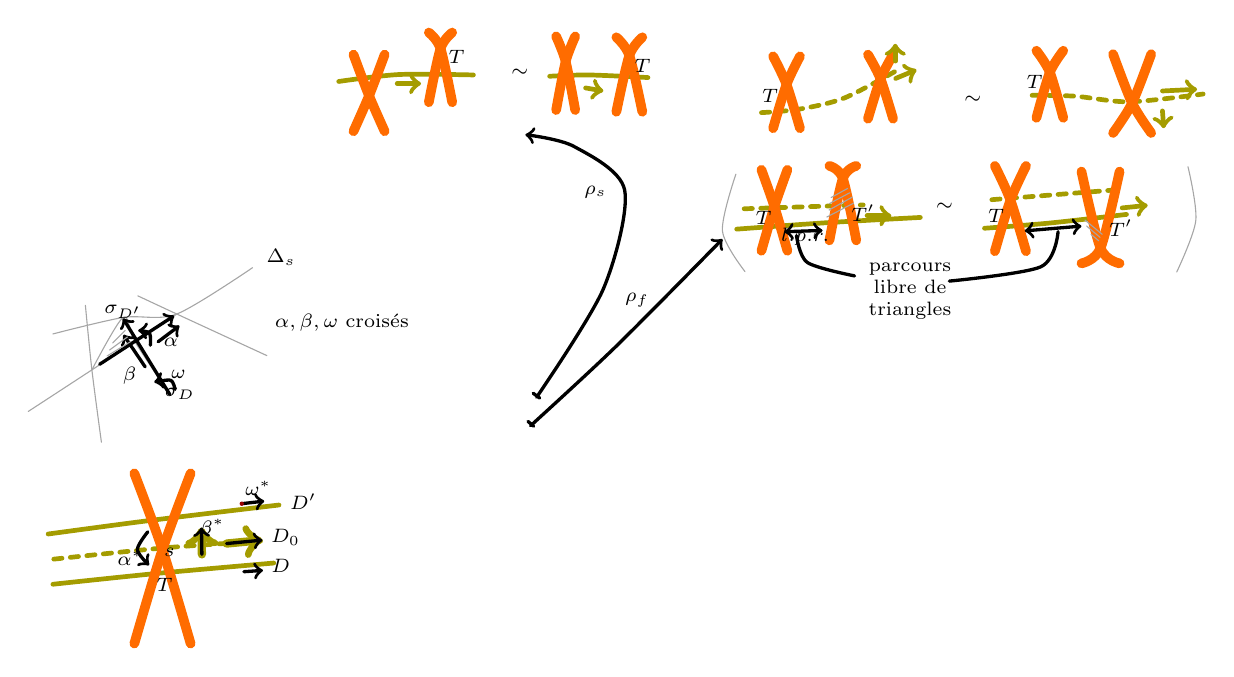
\begin{tikzpicture}[x=.55cm,y=-.55cm,line cap=round,line join=round,g/.style={olive!80!yellow,line width=1.7pt},r/.style={orange!80!brown,line width=1.8pt},w/.style={red!60!black,line width=1.5pt},b/.style={blue!60!black,line width=1.4pt},p/.style={gray!70,thin},k/.style={black,line width=1.2pt},every node/.style={font=\scriptsize}]
\draw[g] plot[smooth] coordinates {(7.97,2.84) (9.36,2.68) (11.08,2.69)};
\draw[orange!85!red,line width=3.5pt] plot[smooth] coordinates {(8.31,2.2199999999999998) (8.67,3.17) (9.03,3.9899999999999998)};
\draw[orange!85!red,line width=3.5pt] plot[smooth] coordinates {(9.03,2.2199999999999998) (8.67,3.17) (8.31,3.9899999999999998)};
\draw[orange!85!red,line width=3.5pt] plot[smooth] coordinates {(10.05,1.71) (10.32,2.08) (10.59,3.3200000000000003)};
\draw[orange!85!red,line width=3.5pt] plot[smooth] coordinates {(10.59,1.71) (10.32,2.08) (10.05,3.3200000000000003)};
\draw[g,->] plot[smooth] coordinates {(9.32,2.89) (9.87,2.89)};
\node at (10.69,2.28) {$T$};
\node at (12.15,2.65) {$\sim$};
\draw[g] plot[smooth] coordinates {(12.84,2.72) (13.74,2.69) (15.11,2.75)};
\draw[orange!85!red,line width=3.5pt] plot[smooth] coordinates {(12.99,1.7999999999999998) (13.21,2.38) (13.430000000000001,3.5)};
\draw[orange!85!red,line width=3.5pt] plot[smooth] coordinates {(13.430000000000001,1.7999999999999998) (13.21,2.38) (12.99,3.5)};
\draw[orange!85!red,line width=3.5pt] plot[smooth] coordinates {(14.379999999999999,1.8200000000000003) (14.68,2.24) (14.98,3.54)};
\draw[orange!85!red,line width=3.5pt] plot[smooth] coordinates {(14.98,1.8200000000000003) (14.68,2.24) (14.379999999999999,3.54)};
\draw[g,->] plot[smooth] coordinates {(13.67,2.99) (14.08,3.06)};
\node at (14.99,2.47) {$T$};
\draw[g,dashed] plot[smooth] coordinates {(17.73,3.56) (18.6,3.48) (19.65,3.22) (20.92,2.55)};
\draw[orange!85!red,line width=3.5pt] plot[smooth] coordinates {(18.0,2.2600000000000002) (18.31,2.91) (18.619999999999997,3.92)};
\draw[orange!85!red,line width=3.5pt] plot[smooth] coordinates {(18.619999999999997,2.2600000000000002) (18.31,2.91) (18.0,3.92)};
\draw[orange!85!red,line width=3.5pt] plot[smooth] coordinates {(20.19,2.2199999999999998) (20.48,2.78) (20.77,3.6999999999999997)};
\draw[orange!85!red,line width=3.5pt] plot[smooth] coordinates {(20.77,2.2199999999999998) (20.48,2.78) (20.19,3.6999999999999997)};
\draw[g,->] plot[smooth] coordinates {(20.82,2.37) (20.82,1.97)};
\draw[g,->] plot[smooth] coordinates {(20.83,2.77) (21.31,2.57)};
\node at (17.93,3.17) {$T$};
\node at (22.61,3.27) {$\sim$};
\draw[g,dashed] plot[smooth] coordinates {(23.98,3.16) (24.97,3.18) (26.23,3.31) (27.93,3.13)};
\draw[orange!85!red,line width=3.5pt] plot[smooth] coordinates {(24.080000000000002,2.13) (24.39,2.63) (24.7,3.6799999999999997)};
\draw[orange!85!red,line width=3.5pt] plot[smooth] coordinates {(24.7,2.13) (24.39,2.63) (24.080000000000002,3.6799999999999997)};
\draw[orange!85!red,line width=3.5pt] plot[smooth] coordinates {(25.849999999999998,2.21) (26.29,3.34) (26.73,4.029999999999999)};
\draw[orange!85!red,line width=3.5pt] plot[smooth] coordinates {(26.73,2.21) (26.29,3.34) (25.849999999999998,4.029999999999999)};
\draw[g,->] plot[smooth] coordinates {(26.99,3.06) (27.79,3.02)};
\draw[g,->] plot[smooth] coordinates {(26.99,3.52) (27.02,3.92)};
\node at (24.04,2.86) {$T$};
\draw[g] plot[smooth] coordinates {(17.16,6.25) (19.26,6.1) (21.4,5.98)};
\draw[g] plot[smooth] coordinates {(22.88,6.23) (24.38,6.11) (26.16,5.91)};
\draw[g,dashed] plot[smooth] coordinates {(17.33,5.78) (20.08,5.69)};
\draw[g,dashed] plot[smooth] coordinates {(23.05,5.57) (25.83,5.35)};
\draw[orange!85!red,line width=3.5pt] plot[smooth] coordinates {(17.73,4.880000000000001) (18.03,5.73) (18.330000000000002,6.75)};
\draw[orange!85!red,line width=3.5pt] plot[smooth] coordinates {(18.330000000000002,4.880000000000001) (18.03,5.73) (17.73,6.75)};
\draw[orange!85!red,line width=3.5pt] plot[smooth] coordinates {(19.3,4.79) (19.61,5.08) (19.919999999999998,6.51)};
\draw[orange!85!red,line width=3.5pt] plot[smooth] coordinates {(19.919999999999998,4.79) (19.61,5.08) (19.3,6.51)};
\draw[orange!85!red,line width=3.5pt] plot[smooth] coordinates {(23.12,4.79) (23.48,5.58) (23.84,6.76)};
\draw[orange!85!red,line width=3.5pt] plot[smooth] coordinates {(23.84,4.79) (23.48,5.58) (23.12,6.76)};
\draw[orange!85!red,line width=3.5pt] plot[smooth] coordinates {(25.119999999999997,4.92) (25.56,6.69) (26.0,7.04)};
\draw[orange!85!red,line width=3.5pt] plot[smooth] coordinates {(26.0,4.92) (25.56,6.69) (25.119999999999997,7.04)};
\draw[p] plot[smooth] coordinates {(19.34,5.52) (19.72,5.31)};
\draw[p] plot[smooth] coordinates {(19.3,5.66) (19.77,5.41)};
\draw[p] plot[smooth] coordinates {(19.29,5.81) (19.83,5.51)};
\draw[p] plot[smooth] coordinates {(19.24,5.97) (19.86,5.65)};
\draw[p] plot[smooth] coordinates {(25.2,6.04) (25.6,6.37)};
\draw[p] plot[smooth] coordinates {(25.24,6.18) (25.55,6.44)};
\draw[p] plot[smooth] coordinates {(25.34,6.37) (25.52,6.52)};
\draw[g,->] plot[smooth] coordinates {(20.17,5.94) (20.73,5.94)};
\draw[g,->] plot[smooth] coordinates {(26.06,5.76) (26.65,5.7)};
\draw[k,<->] plot[smooth] coordinates {(18.26,6.31) (19.14,6.28)};
\draw[k,<->] plot[smooth] coordinates {(23.81,6.29) (25.12,6.18)};
\node at (17.78,6.0) {$T$};
\node at (20.08,5.88) {$T'$};
\node at (23.15,5.94) {$T$};
\node at (26.03,6.23) {$T'$};
\node at (21.96,5.73) {$\sim$};
\node at (18.74,6.43) {$\unsure{l.p.r.}$};
\draw[p] plot[smooth] coordinates {(17.14,4.98) (16.83,6.29) (17.35,7.23)};
\draw[p] plot[smooth] coordinates {(27.58,4.81) (27.76,6.05) (27.32,7.24)};
\draw[k] plot[smooth] coordinates {(18.54,6.4) (18.79,7.02) (19.88,7.33)};
\draw[k] plot[smooth] coordinates {(24.58,6.31) (24.18,7.12) (22.07,7.45)};
\node[align=center] at (21.16,7.69) {parcours\\ libre de\\ triangles};
\draw[k,->] plot[smooth] coordinates {(12.54,10.13) (14.08,7.63) (14.57,5.34) (13.4,4.34) (12.28,4.07)};
\draw[k,->] plot[smooth] coordinates {(12.4,10.79) (14.37,8.96) (16.83,6.48)};
\draw[k] plot[smooth] coordinates {(12.46,10.04) (12.61,10.15)};
\draw[k] plot[smooth] coordinates {(12.34,10.69) (12.47,10.8)};
\node at (13.9,5.39) {$\rho_s$};
\node at (14.86,7.88) {$\rho_f$};
\draw[p] plot[smooth] coordinates {(1.37,8.67) (2.99,8.29) (4.23,8.21) (5.98,7.14)};
\draw[p] plot[smooth] coordinates {(3.33,7.79) (4.23,8.21) (6.31,9.17)};
\draw[p] plot[smooth] coordinates {(2.12,8.01) (2.27,9.5) (2.49,11.17)};
\draw[p] plot[smooth] coordinates {(2.27,9.5) (2.99,8.29) (3.27,8.86) (4.07,10.07)};
\draw[p] plot[smooth] coordinates {(.8,10.46) (2.27,9.5) (4.23,8.21)};
\draw[k,->] plot[smooth] coordinates {(2.45,9.37) (4.17,8.25)};
\draw[k,->] plot[smooth] coordinates {(4.07,10.07) (2.99,8.31)};
\draw[k,->] plot[smooth] coordinates {(3.5,9.43) (3.0,8.69)};
\draw[k,->] plot[smooth] coordinates {(3.8,8.85) (4.29,8.48)};
\draw[k,->] plot[smooth] coordinates {(3.62,8.93) (3.6,8.65) (3.34,8.59)};
\draw[k,->] plot[smooth] coordinates {(4.19,9.95) (4.09,9.74) (3.71,9.78)};
\draw[p] plot[smooth] coordinates {(2.62,9.18) (3.16,8.85)};
\draw[p] plot[smooth] coordinates {(2.68,9.04) (3.09,8.74)};
\draw[p] plot[smooth] coordinates {(2.75,8.88) (3.04,8.59)};
\node at (6.64,6.9) {$\Delta_s$};
\node at (2.99,8.15) {$\sigma_{D'}$};
\node at (4.3,10.06) {$\sigma_D$};
\node at (4.27,9.6) {$\omega$};
\node at (3.14,9.64) {$\beta$};
\node at (4.09,8.86) {$\alpha$};
\node[anchor=west] at (6.27,8.4) {$\alpha,\beta,\omega$ croisés};
\draw[g] plot[smooth] coordinates {(1.26,13.29) (3.59,12.98) (6.59,12.62)};
\draw[g,dashed] plot[smooth] coordinates {(1.39,13.87) (3.94,13.61) (6.24,13.45)};
\draw[g] plot[smooth] coordinates {(1.37,14.45) (3.77,14.2) (6.47,13.96)};
\draw[orange!85!red,line width=3.5pt] plot[smooth] coordinates {(3.25,11.89) (3.9,13.65) (4.55,15.82)};
\draw[orange!85!red,line width=3.5pt] plot[smooth] coordinates {(4.55,11.89) (3.9,13.65) (3.25,15.82)};
\draw[g,->,line width=3pt] plot[smooth] coordinates {(4.81,13.76) (4.8,13.14)};
\draw[g,->,line width=3pt] plot[smooth] coordinates {(5.38,13.51) (6.21,13.43)};
\draw[k,->] plot[smooth] coordinates {(4.81,13.76) (4.8,13.14)};
\draw[k,->] plot[smooth] coordinates {(5.38,13.51) (6.21,13.43)};
\draw[k,->] plot[smooth] coordinates {(5.73,12.59) (6.25,12.53)};
\draw[k,->] plot[smooth] coordinates {(5.78,14.16) (6.22,14.13)};
\draw[k,->] plot[smooth] coordinates {(3.56,13.24) (3.32,13.65) (3.59,14.01)};
\fill[w] (5.73,12.59) circle (.05);
\node at (6.74,13.36) {$D_0$};
\node at (6.63,14.02) {$D$};
\node at (7.15,12.54) {$D'$};
\node at (6.11,12.24) {$\omega^*$};
\node at (5.04,13.17) {$\beta^*$};
\node at (3.16,13.85) {$\alpha^*$};
\node at (4.06,13.72) {$s$};
\node at (3.95,14.46) {$T$};
\end{tikzpicture}}
\diagram{\begin{tikzcd}[ampersand replacement=\&,row sep=2.5em,column sep=3em]
\begin{gathered}\figure{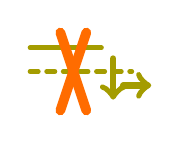
\begin{tikzpicture}[x=.55cm,y=-.55cm,line cap=round,line join=round,g/.style={olive!80!yellow,line width=1.7pt},r/.style={orange!80!brown,line width=1.8pt},w/.style={red!60!black,line width=1.5pt},b/.style={blue!60!black,line width=1.4pt},p/.style={gray!70,thin},k/.style={black,line width=1.2pt},every node/.style={font=\scriptsize}]
\draw[g,dashed] plot[smooth] coordinates {(0,0) (2.35,0)};
\draw[g] plot[smooth] coordinates {(0,-0.55) (1.65,-0.55)};
\draw[orange!85!red,line width=3.5pt] plot[smooth] coordinates {(0.7,-0.9) (1,0) (1.3,0.9)};
\draw[orange!85!red,line width=3.5pt] plot[smooth] coordinates {(1.3,-0.9) (1,0) (0.7,0.9)};
\draw[g,->,line width=2.3pt] plot[smooth] coordinates {(1.92,-0.3) (1.92,0.65)};
\draw[g,->,line width=2.3pt] plot[smooth] coordinates {(2.15,.32) (2.8,.32)};
\end{tikzpicture}}
\\(D_0,-\beta^*,\omega^*)\end{gathered} \& \\
{} \& \begin{gathered}\figure{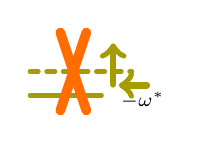
\begin{tikzpicture}[execute at begin node={\ifmmode$\fi},execute at end node={\ifmmode$\fi},x=.55cm,y=-.55cm,line cap=round,line join=round,g/.style={olive!80!yellow,line width=1.7pt},r/.style={orange!80!brown,line width=1.8pt},w/.style={red!60!black,line width=1.5pt},b/.style={blue!60!black,line width=1.4pt},p/.style={gray!70,thin},k/.style={black,line width=1.2pt},every node/.style={font=\scriptsize}]
\draw[g,dashed] plot[smooth] coordinates {(0,0) (2.35,0)};
\draw[g] plot[smooth] coordinates {(0,0.55) (1.65,0.55)};
\draw[orange!85!red,line width=3.5pt] plot[smooth] coordinates {(0.7,-0.9) (1,0) (1.3,0.9)};
\draw[orange!85!red,line width=3.5pt] plot[smooth] coordinates {(1.3,-0.9) (1,0) (0.7,0.9)};
\draw[g,->,line width=2.3pt] plot[smooth] coordinates {(1.92,0.3) (1.92,-0.65)};
\draw[g,->,line width=2.3pt] plot[smooth] coordinates {(2.7,.32) (2.05,.32)};
\node at (2.6,.67) {$-\omega^*$};
\end{tikzpicture}}
\\(D_0,\beta^*,-\omega^*)\end{gathered} \\
(D_0,\beta^*\omega^*) \arrow[uu,"\sigma",mapsto] \arrow[ur,"\sigma_0",mapsto] \arrow[r,"\sigma_1",mapsto] \arrow[dr,"\sigma_2",mapsto] \& \figure{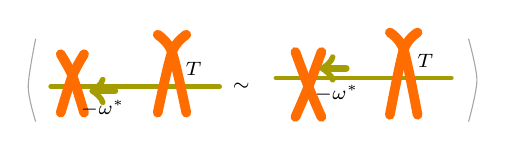
\begin{tikzpicture}[execute at begin node={\ifmmode$\fi},execute at end node={\ifmmode$\fi},x=.55cm,y=-.55cm,line cap=round,line join=round,g/.style={olive!80!yellow,line width=1.7pt},r/.style={orange!80!brown,line width=1.8pt},w/.style={red!60!black,line width=1.5pt},b/.style={blue!60!black,line width=1.4pt},p/.style={gray!70,thin},k/.style={black,line width=1.2pt},every node/.style={font=\scriptsize}]
\draw[g] plot[smooth] coordinates {(0,0) (3.9,0)};
\draw[orange!85!red,line width=3.5pt] plot[smooth] coordinates {(0.22999999999999998,-0.75) (0.5,-0.25) (0.77,0.6)};
\draw[orange!85!red,line width=3.5pt] plot[smooth] coordinates {(0.77,-0.75) (0.5,-0.25) (0.22999999999999998,0.6)};
\draw[orange!85!red,line width=3.5pt] plot[smooth] coordinates {(2.4699999999999998,-1.2000000000000002) (2.8,-0.8) (3.13,0.5999999999999999)};
\draw[orange!85!red,line width=3.5pt] plot[smooth] coordinates {(3.13,-1.2000000000000002) (2.8,-0.8) (2.4699999999999998,0.5999999999999999)};
\draw[g,<-,line width=2.5pt] plot[smooth] coordinates {(.89,.1) (1.48,.1)};
\node at (1.2,.5) {$-\omega^*$};
\node at (3.3,-.4) {$T$};
\node at (4.4,0) {$\sim$};
\draw[g] plot[smooth] coordinates {(5.2,-.2) (9.25,-.2)};
\draw[orange!85!red,line width=3.5pt] plot[smooth] coordinates {(5.65,-0.8) (5.95,0) (6.25,0.7)};
\draw[orange!85!red,line width=3.5pt] plot[smooth] coordinates {(6.25,-0.8) (5.95,0) (5.65,0.7)};
\draw[orange!85!red,line width=3.5pt] plot[smooth] coordinates {(7.83,-1.25) (8.15,-0.85) (8.47,0.65)};
\draw[orange!85!red,line width=3.5pt] plot[smooth] coordinates {(8.47,-1.25) (8.15,-0.85) (7.83,0.65)};
\draw[g,<-,line width=2.5pt] plot[smooth] coordinates {(6.2,-.42) (6.82,-.42)};
\node at (6.6,.15) {$-\omega^*$};
\node at (8.65,-.6) {$T$};
\draw[p] plot[smooth] coordinates {(-.35,-1.1) (-.52,0) (-.35,.8)};
\draw[p] plot[smooth] coordinates {(9.65,-1.1) (9.84,-.15) (9.65,.8)};
\end{tikzpicture}}
 \\
\& \begin{gathered}\figure{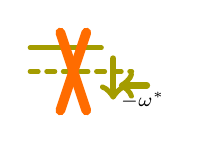
\begin{tikzpicture}[execute at begin node={\ifmmode$\fi},execute at end node={\ifmmode$\fi},x=.55cm,y=-.55cm,line cap=round,line join=round,g/.style={olive!80!yellow,line width=1.7pt},r/.style={orange!80!brown,line width=1.8pt},w/.style={red!60!black,line width=1.5pt},b/.style={blue!60!black,line width=1.4pt},p/.style={gray!70,thin},k/.style={black,line width=1.2pt},every node/.style={font=\scriptsize}]
\draw[g,dashed] plot[smooth] coordinates {(0,0) (2.35,0)};
\draw[g] plot[smooth] coordinates {(0,-0.55) (1.65,-0.55)};
\draw[orange!85!red,line width=3.5pt] plot[smooth] coordinates {(0.7,-0.9) (1,0) (1.3,0.9)};
\draw[orange!85!red,line width=3.5pt] plot[smooth] coordinates {(1.3,-0.9) (1,0) (0.7,0.9)};
\draw[g,->,line width=2.3pt] plot[smooth] coordinates {(1.92,-0.3) (1.92,0.65)};
\draw[g,->,line width=2.3pt] plot[smooth] coordinates {(2.7,.32) (2.05,.32)};
\node at (2.6,.67) {$-\omega^*$};
\end{tikzpicture}}
\\(D_0,-\beta^*,-\omega^*)\end{gathered}
\end{tikzcd}}

$\alpha^*,\beta^*,\omega^*$ \uline{non} croisés
\[
\omega^*=-\alpha^*\wedge\beta^*\qquad
\omega=\alpha\wedge\beta
\]
$\sigma_0$ donc change $\alpha$ en $-\alpha$, en gardant $\sigma_D,\sigma_{D'},\beta$.

$\sigma_2$ échange $\sigma_D$ et $\sigma_{D'}$, change $\beta$ en $-\beta$, garde $\alpha$.
\margin{\mspage{156}}

\scanpage{158}
\figure{
\begin{tikzpicture}[x=.55cm,y=-.55cm,line cap=round,line join=round,g/.style={olive!80!yellow,line width=1.7pt},r/.style={orange!80!brown,line width=1.8pt},w/.style={red!60!black,line width=1.5pt},b/.style={blue!60!black,line width=1.4pt},p/.style={gray!70,thin},k/.style={black,line width=1.2pt},every node/.style={font=\scriptsize}]
\draw[brown!50,line width=3pt] (1.04,1.28)--(1.05,1.69);
\draw[purple!40,line width=3pt] (1.36,1.31)--(1.4,1.7);
\draw[yellow!85!orange,line width=3pt] (1.57,1.38)--(1.65,1.88);
\draw[orange!90!red,line width=3pt] (1.83,.98)--(1.87,1.48);
\draw[orange!90!red,line width=3pt] (2.07,1.27)--(2.13,1.84);
\draw[red!70!brown,line width=3pt] (2.43,1.25)--(2.5,1.96);
\draw[orange!80!brown,line width=3pt] (2.76,1.3)--(2.84,1.99);
\draw[purple!30,line width=3pt] (3.19,1.32)--(3.22,2.04);
\draw[orange!90!red,line width=3pt] (3.48,1.29)--(3.48,1.84);
\draw[orange!90!red,line width=3pt] (4.43,1.09)--(4.39,1.68);
\draw[yellow!70!green,line width=3pt] (4.8,1.2)--(4.77,1.79);
\draw[teal!50,line width=3pt] (5.13,1.26)--(5.06,1.81);
\draw[g,line width=3pt] (5.48,1.45)--(5.43,1.98);
\end{tikzpicture}}

$X,\check X$ plans projectifs réels duaux

$T$ \deleted{\unsure{système de trois droites}} \inserted{``triangle'' \unsure{de} $X$}, $T'$ triangle dual dans $\check X$

\deleted{\unsure{étant des}}
alors les orientations de $T$ et $T'$ se correspondent, de façon que si $\omega$ et $\omega'$ sont associées, d'où des orientations des \deleted{\unsure{trois}} droites \unsure{d'épure|d'équerre} de $T$ et de $T'$, et de $X$ resp. $\check X$ en les sommets de $T$, resp. $T'$, alors pour un \deleted{pt} \inserted{sommet} de $X$ -- $\check X$ et la droite corresp. de $\check X$ -- $X$, les orientations se correspondent.
\figure{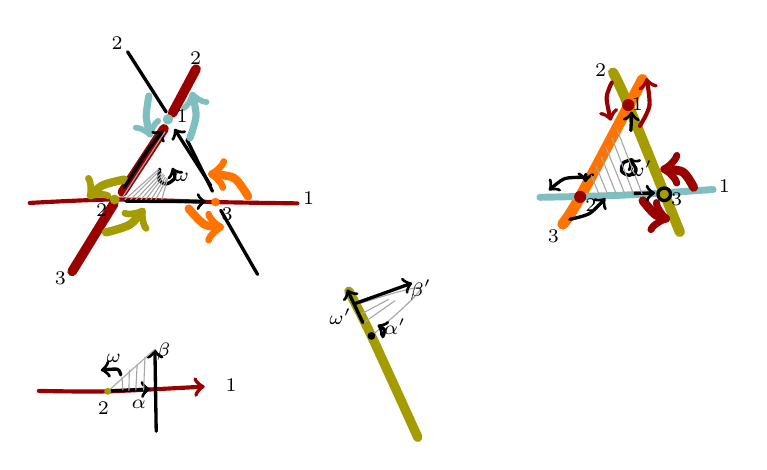
\begin{tikzpicture}[x=.55cm,y=-.55cm,line cap=round,line join=round,g/.style={olive!80!yellow,line width=1.7pt},r/.style={orange!80!brown,line width=1.8pt},w/.style={red!60!black,line width=1.5pt},b/.style={blue!60!black,line width=1.4pt},p/.style={gray!70,thin},k/.style={black,line width=1.2pt},every node/.style={font=\scriptsize}]
\draw[w] plot[smooth] coordinates {(1.4,7.18) (3.36,7.1) (5.69,7.16) (7.58,7.19)};
\draw[w,line width=3.5pt] plot[smooth] coordinates {(2.38,8.76) (3.34,7.2)};
\draw[w,line width=3.5pt] plot[smooth] coordinates {(3.54,6.93) (4.5,5.47)};
\draw[w,line width=3.5pt] plot[smooth] coordinates {(4.7,5.1) (5.24,4.09)};
\draw[k] plot[smooth] coordinates {(3.66,3.69) (4.55,5.08)};
\draw[k] plot[smooth] coordinates {(5.03,5.72) (5.62,6.91)};
\draw[k] plot[smooth] coordinates {(5.81,7.35) (6.66,8.83)};
\draw[teal!50,line width=2.6pt,->] plot[smooth] coordinates {(4.15,4.71) (4.09,5.2) (4.2,5.67)};
\draw[teal!50,line width=2.6pt,->] plot[smooth] coordinates {(5.1,5.68) (5.24,5.16) (5.14,4.61)};
\draw[g,->,line width=3pt] plot[smooth] coordinates {(3.58,6.64) (3.07,6.78) (2.74,7.08)};
\draw[g,->,line width=3pt] plot[smooth] coordinates {(3.16,7.86) (3.71,7.68) (4.05,7.3)};
\draw[orange!90!red,->,line width=3pt] plot[smooth] coordinates {(6.44,7.03) (6.11,6.6) (5.51,6.51)};
\draw[orange!90!red,->,line width=3pt] plot[smooth] coordinates {(5.07,7.31) (5.44,7.68) (5.89,7.74)};
\draw[k,->] plot[smooth] coordinates {(3.58,6.83) (4.1,6.0) (4.48,5.51)};
\draw[k,->] plot[smooth] coordinates {(5.58,6.78) (4.74,5.47)};
\draw[k,->] plot[smooth] coordinates {(3.62,7.14) (5.47,7.15)};
\draw[k,->] plot[smooth] coordinates {(4.4,6.4) (4.39,6.65) (4.56,6.74) (4.75,6.6) (4.69,6.37)};
\draw[p] plot[smooth] coordinates {(3.54,7.05) (4.52,5.54)};
\draw[p] plot[smooth] coordinates {(3.6,7.1) (4.38,6.4)};
\draw[p] plot[smooth] coordinates {(3.73,7.1) (4.4,6.43)};
\draw[p] plot[smooth] coordinates {(3.85,7.1) (4.44,6.48)};
\draw[p] plot[smooth] coordinates {(3.97,7.1) (4.48,6.51)};
\draw[p] plot[smooth] coordinates {(4.08,7.1) (4.51,6.54)};
\draw[p] plot[smooth] coordinates {(4.2,7.1) (4.53,6.59)};
\draw[p] plot[smooth] coordinates {(4.31,7.1) (4.57,6.61)};
\draw[p] plot[smooth] coordinates {(4.45,7.1) (4.58,6.63)};
\fill[g] (3.36,7.1) circle (.115);
\fill[orange!90!red] (5.69,7.16) circle (.1);
\fill[teal!50] (4.59,5.25) circle (.12);
\node at (3.42,3.49) {$2$};
\node at (5.23,3.84) {$2$};
\node at (4.92,5.18) {$1$};
\node at (7.84,7.08) {$1$};
\node at (2.11,8.93) {$3$};
\node at (3.06,7.35) {$2$};
\node at (5.96,7.45) {$3$};
\node at (4.91,6.6) {$\omega$};
\draw[g,line width=3.7pt] plot[smooth] coordinates {(14.87,4.17) (15.22,4.92) (16.41,7.85)};
\draw[orange!90!red,line width=4pt] plot[smooth] coordinates {(15.55,4.33) (14.11,7.04) (13.71,7.67)};
\draw[teal!50,line width=2.5pt] plot[smooth] coordinates {(13.18,7.05) (15.1,7.0) (17.18,6.87)};
\draw[w,->] plot[smooth] coordinates {(14.84,4.4) (14.72,4.75) (14.82,5.28)};
\draw[w,->] plot[smooth] coordinates {(15.49,5.4) (15.71,4.93) (15.64,4.3)};
\draw[w,->,line width=3.2pt] plot[smooth] coordinates {(16.73,6.82) (16.47,6.46) (15.96,6.4)};
\draw[w,->,line width=3.2pt] plot[smooth] coordinates {(15.56,7.13) (15.85,7.45) (16.18,7.56)};
\draw[k,->] plot[smooth] coordinates {(14.23,6.59) (13.75,6.62) (13.39,6.89)};
\draw[k,->] plot[smooth] coordinates {(13.87,7.56) (14.33,7.42) (14.69,7.07)};
\draw[k,->] plot[smooth] coordinates {(14.24,6.52) (14.23,6.7)};
\draw[k,->] plot[smooth] coordinates {(15.28,5.51) (15.3,5.07)};
\draw[k,->] plot[smooth] coordinates {(15.36,6.96) (15.84,6.95)};
\draw[k,->] plot[smooth] coordinates {(15.31,6.18) (15.11,6.25) (15.07,6.45) (15.25,6.54) (15.4,6.4) (15.24,6.17)};
\draw[p] plot[smooth] coordinates {(14.37,6.55) (14.54,6.97)};
\draw[p] plot[smooth] coordinates {(14.48,6.34) (14.74,6.97)};
\draw[p] plot[smooth] coordinates {(14.6,6.11) (14.94,6.97)};
\draw[p] plot[smooth] coordinates {(14.7,5.88) (15.14,6.97)};
\draw[p] plot[smooth] coordinates {(14.84,5.67) (15.34,6.97)};
\draw[p] plot[smooth] coordinates {(14.96,5.48) (15.54,6.97)};
\fill[w] (15.22,4.92) circle (.14);
\fill[w] (14.11,7.04) circle (.14);
\fill[g] (16.05,6.98) circle (.11);
\draw[k] (16.05,6.98) circle (.145);
\node at (14.58,4.12) {$2$};
\node at (15.43,4.89) {$1$};
\node at (17.44,6.8) {$1$};
\node at (14.36,7.23) {$2$};
\node at (16.34,7.1) {$3$};
\node at (13.49,7.95) {$3$};
\node at (15.52,6.39) {$\omega'$};
\draw[w,->] plot[smooth] coordinates {(1.61,11.52) (3.2,11.53) (5.44,11.42)};
\draw[k,->] plot[smooth] coordinates {(4.32,12.45) (4.29,10.56)};
\draw[k,->] plot[smooth] coordinates {(3.24,11.52) (4.18,11.48)};
\draw[k,->] plot[smooth] coordinates {(3.5,11.15) (3.42,11.02) (3.04,11.04)};
\draw[p] plot[smooth] coordinates {(3.2,11.53) (4.29,10.56)};
\draw[p] plot[smooth] coordinates {(3.55,11.5) (3.53,11.21)};
\draw[p] plot[smooth] coordinates {(3.69,11.51) (3.7,11.04)};
\draw[p] plot[smooth] coordinates {(3.85,11.5) (3.88,10.91)};
\draw[p] plot[smooth] coordinates {(4.03,11.5) (4.06,10.74)};
\fill[g] (3.2,11.53) circle (.08);
\node at (3.34,10.76) {$\omega$};
\node at (4.49,10.62) {$\beta$};
\node at (3.92,11.82) {$\alpha$};
\node at (6.05,11.39) {$1$};
\node at (3.1,11.91) {$2$};
\draw[g,line width=3.4pt] plot[smooth] coordinates {(8.77,9.22) (9.29,10.25) (10.36,12.59)};
\draw[p] plot[smooth] coordinates {(9.29,10.25) (10.42,9.15) (8.88,9.55)};
\draw[p] plot[smooth] coordinates {(9.12,9.94) (9.83,9.44)};
\draw[p] plot[smooth] coordinates {(9.04,9.75) (9.68,9.41)};
\draw[k,->] plot[smooth] coordinates {(8.92,9.5) (10.23,9.03)};
\draw[k,->] plot[smooth] coordinates {(9.09,9.94) (8.73,9.18)};
\draw[k,->] plot[smooth] coordinates {(9.55,10.27) (9.59,10.11) (9.43,10.0)};
\fill[k] (9.29,10.25) circle (.09);
\node at (8.57,9.81) {$\omega'$};
\node at (10.43,9.19) {$\beta'$};
\node at (9.83,10.03) {$\alpha'$};
\end{tikzpicture}}
$\alpha,\beta,\omega$ associés,
mais $\alpha',\beta',\omega'$ \uline{non associés}.
\figure{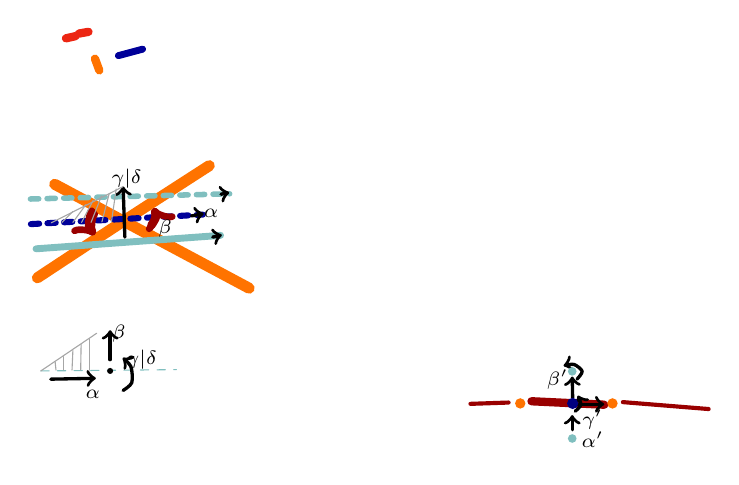
\begin{tikzpicture}[x=.55cm,y=-.55cm,line cap=round,line join=round,g/.style={olive!80!yellow,line width=1.7pt},r/.style={orange!80!brown,line width=1.8pt},w/.style={red!60!black,line width=1.5pt},b/.style={blue!60!black,line width=1.4pt},p/.style={gray!70,thin},k/.style={black,line width=1.2pt},every node/.style={font=\scriptsize}]
\draw[red!70!brown,line width=3pt] plot[smooth] coordinates {(1.88,15.7) (2.1,15.65)};
\draw[red!70!brown,line width=3pt] plot[smooth] coordinates {(2.18,15.59) (2.4,15.55)};
\draw[orange!90!red,line width=3pt] plot[smooth] coordinates {(2.55,16.17) (2.65,16.44)};
\draw[blue!60!black,line width=2.5pt] plot[smooth] coordinates {(3.09,16.1) (3.65,15.95)};
\draw[orange!90!red,line width=4pt] plot[smooth] coordinates {(1.62,19.07) (3.21,19.92) (6.11,21.47)};
\draw[orange!90!red,line width=4pt] plot[smooth] coordinates {(1.22,21.23) (3.21,19.92) (5.19,18.64)};
\draw[teal!50,line width=2.5pt] plot[smooth] coordinates {(1.19,20.56) (5.45,20.25)};
\draw[teal!50,dashed,line width=2pt] plot[smooth] coordinates {(1.06,19.41) (5.66,19.29)};
\draw[blue!60!black,dashed,line width=2.2pt] plot[smooth] coordinates {(1.07,19.99) (5.04,19.77)};
\draw[k,->] plot[smooth] coordinates {(3.24,20.29) (3.2,19.12)};
\draw[k,->] plot[smooth] coordinates {(5.27,20.29) (5.48,20.24)};
\draw[k,->] plot[smooth] coordinates {(5.46,19.3) (5.65,19.26)};
\draw[k,->] plot[smooth] coordinates {(4.78,19.8) (5.06,19.75)};
\draw[w,->,line width=3pt] plot[smooth] coordinates {(2.47,19.7) (2.41,20.01) (2.54,20.23)};
\draw[w,->,line width=3pt] plot[smooth] coordinates {(3.85,20.02) (3.96,19.82) (3.9,19.64)};
\draw[p] plot[smooth] coordinates {(1.54,19.96) (3.19,19.13)};
\draw[p] plot[smooth] coordinates {(1.79,19.95) (2.04,19.7)};
\draw[p] plot[smooth] coordinates {(2.04,19.95) (2.34,19.54)};
\draw[p] plot[smooth] coordinates {(2.24,19.95) (2.51,19.44)};
\draw[p] plot[smooth] coordinates {(2.46,19.95) (2.7,19.34)};
\draw[p] plot[smooth] coordinates {(2.71,19.94) (2.88,19.28)};
\draw[p] plot[smooth] coordinates {(2.93,19.94) (3.04,19.18)};
\node at (3.28,18.95) {$\unsure{\gamma|\delta}$};
\node at (5.23,19.75) {$\alpha$};
\node at (4.17,20.09) {$\beta$};
\draw[teal!50,dashed] plot[smooth] coordinates {(1.3,23.38) (4.43,23.35)};
\draw[k,->] plot[smooth] coordinates {(1.53,23.57) (2.57,23.55)};
\draw[k,->] plot[smooth] coordinates {(2.9,23.12) (2.9,22.44)};
\draw[k,->] plot[smooth] coordinates {(3.2,23.83) (3.4,23.65) (3.38,23.28) (3.19,23.08)};
\draw[p] plot[smooth] coordinates {(1.3,23.38) (2.59,22.51)};
\draw[p] plot[smooth] coordinates {(1.65,23.36) (1.63,23.17)};
\draw[p] plot[smooth] coordinates {(1.83,23.36) (1.83,23.05)};
\draw[p] plot[smooth] coordinates {(2.02,23.36) (2.04,22.91)};
\draw[p] plot[smooth] coordinates {(2.22,23.36) (2.23,22.77)};
\draw[p] plot[smooth] coordinates {(2.43,23.36) (2.43,22.64)};
\fill[k] (2.9,23.38) circle (.07);
\node at (2.5,23.91) {$\alpha$};
\node at (3.1,22.52) {$\beta$};
\node at (3.63,23.12) {$\unsure{\gamma|\delta}$};
\draw[w] plot[smooth] coordinates {(11.22,24.14) (12.1,24.11)};
\draw[w] plot[smooth] coordinates {(14.74,24.1) (16.72,24.26)};
\draw[w,line width=3pt] plot[smooth] coordinates {(12.63,24.08) (14.31,24.16)};
\draw[k,->] plot[smooth] coordinates {(13.58,24.0) (13.57,23.51)};
\draw[k,->] plot[smooth] coordinates {(13.57,24.74) (13.57,24.4)};
\draw[k,->] plot[smooth] coordinates {(13.67,24.15) (14.31,24.15)};
\draw[k,->] plot[smooth] coordinates {(13.68,23.57) (13.8,23.39) (13.61,23.23) (13.37,23.26)};
\draw[k,->] plot[smooth] coordinates {(13.64,24.31) (13.77,24.16) (13.7,23.95)};
\fill[orange!90!red] (12.37,24.13) circle (.12);
\fill[orange!90!red] (14.5,24.13) circle (.12);
\fill[blue!50!black] (13.58,24.13) circle (.13);
\fill[teal!50] (13.57,23.39) circle (.1);
\fill[teal!50] (13.57,24.94) circle (.1);
\node at (13.23,23.58) {$\beta'$};
\node at (14.04,24.51) {$\unsure{\gamma'}$};
\node at (14.04,24.97) {$\alpha'$};
\end{tikzpicture}}
{\ttfamily\unsure{//*}\quad CRAY2\quad\unsure{0135}\quad I}
{\scriptsize\begin{tabular}{l}
\texttt{\ \ \ \ \ \ \ \ \ \ \ 00000000\ \ \ \ \ \ 00000000\ \ \ \ \ \ 00000000\ \ \ \ \ \ 00000000}\\
\texttt{\ \ \ \ \ \ \ \ \ 0000000000\ \ \ \ 0000000000\ \ \ \ 0000000000\ \ \ \ 0000000000}\\
\texttt{\ \ \ \ \ \ \ 00\ \ \ \ \ \ 0000\ \ 00\ \ \ \ \ \ 0000\ \ 00\ \ \ \ \ \ 0000\ \ 00\ \ \ \ \ \ 0000}\\
\texttt{\ \ \ \ \ \ 00\ \ \ \ \ 00\ 00\ \ 00\ \ \ \ \ 00\ 00\ \ 00\ \ \ \ \ 00\ 00\ \ 00\ \ \ \ \ 00\ 00}\\
\texttt{\ \ \ \ \ 00\ \ \ \ 00\ \ 00\ \ 00\ \ \ \ 00\ \ 00\ \ 00\ \ \ \ 00\ \ 00\ \ 00\ \ \ \ 00\ \ 00}\\
\texttt{\ \ \ \ 00\ \ \ 00\ \ \ 00\ \ 00\ \ \ 00\ \ \ 00\ \ 00\ \ \ 00\ \ \ 00\ \ 00\ \ \ 00\ \ \ 00}\\
\texttt{\ \ \ 00\ \ 00\ \ \ \ 00\ \ 00\ \ 00\ \ \ \ 00\ \ 00\ \ 00\ \ \ \ 00\ \ 00\ \ 00\ \ \ \ 00}\\
\texttt{\ \ 00\ 00\ \ \ \ \ 00\ \ 00\ 00\ \ \ \ \ 00\ \ 00\ 00\ \ \ \ \ 00\ \ 00\ 00\ \ \ \ \ 00}\\
\texttt{\ 0000\ \ \ \ \ \ 00\ \ 0000\ \ \ \ \ \ 00\ \ 0000\ \ \ \ \ \ 00\ \ 0000\ \ \ \ \ \ 00}\\
\texttt{000\ \ \ \ \ \ \ 00\ \ 000\ \ \ \ \ \ \ 00\ \ 000\ \ \ \ \ \ \ 00\ \ 000\ \ \ \ \ \ \ 00}\\
\texttt{0000000000\ \ \ \ 0000000000\ \ \ \ 0000000000\ \ \ \ 0000000000}\\
\texttt{00000000\ \ \ \ \ \ 00000000\ \ \ \ \ \ 00000000\ \ \ \ \ \ 00000000}\\
\texttt{}\\
\texttt{\ CCCCCCCCCC\ \ \ RRRRRRRRRRR\ \ \ AAAAAAAAAA\ \ \ YY\ \ \ \ \ \ \ \ YY\ \ \ 2222222222}\\
\texttt{CCCCCCCCCCCC\ \ RRRRRRRRRRRR\ AAAAAAAAAAAA\ \ YY\ \ \ \ \ \ \ \ YY\ \ 222222222222}\\
\texttt{CC\ \ \ \ \ \ \ \ CC\ \ RR\ \ \ \ \ \ \ \ RR\ AA\ \ \ \ \ \ \ \ AA\ \ YY\ \ \ \ \ \ YY\ \ \ 22\ \ \ \ \ \ \ \ 22}\\
\texttt{CC\ \ \ \ \ \ \ \ \ \ \ \ RR\ \ \ \ \ \ \ \ RR\ AA\ \ \ \ \ \ \ \ AA\ \ \ YY\ \ \ \ YY\ \ \ \ \ \ \ \ \ \ \ \ \ 22}\\
\texttt{CC\ \ \ \ \ \ \ \ \ \ \ \ RR\ \ \ \ \ \ \ \ RR\ AA\ \ \ \ \ \ \ \ AA\ \ \ \ YY\ \ YY\ \ \ \ \ \ \ \ \ \ \ \ \ \ 22}\\
\texttt{CC\ \ \ \ \ \ \ \ \ \ \ \ RRRRRRRRRRRR\ AAAAAAAAAAAA\ \ \ \ \ YYYY\ \ \ \ \ \ \ \ \ \ \ \ \ \ 22}\\
\texttt{CC\ \ \ \ \ \ \ \ \ \ \ \ RRRRRRRRRRR\ \ AAAAAAAAAAAA\ \ \ \ \ \ YY\ \ \ \ \ \ \ \ \ \ \ \ \ \ 22}\\
\texttt{CC\ \ \ \ \ \ \ \ \ \ \ \ RR\ \ \ \ RR\ \ \ \ \ AA\ \ \ \ \ \ \ \ AA\ \ \ \ \ \ YY\ \ \ \ \ \ \ \ \ \ \ \ \ 22}\\
\texttt{CC\ \ \ \ \ \ \ \ \ \ \ \ RR\ \ \ \ \ RR\ \ \ \ AA\ \ \ \ \ \ \ \ AA\ \ \ \ \ \ YY\ \ \ \ \ \ \ \ \ \ \ \ 22}\\
\texttt{CC\ \ \ \ \ \ \ \ CC\ \ RR\ \ \ \ \ \ RR\ \ \ AA\ \ \ \ \ \ \ \ AA\ \ \ \ \ \ YY\ \ \ \ \ \ \ \ \ \ \ 22}\\
\texttt{CCCCCCCCCCCC\ \ RR\ \ \ \ \ \ \ RR\ \ AA\ \ \ \ \ \ \ \ AA\ \ \ \ \ \ YY\ \ \ \ \ \ \ \ \ \ 222222222222}\\
\texttt{\ CCCCCCCCCC\ \ \ RR\ \ \ \ \ \ \ \ RR\ AA\ \ \ \ \ \ \ \ AA\ \ \ \ \ \ YY\ \ \ \ \ \ \ \ \ \ 222222222222}\\
\end{tabular}}
{\ttfamily ****A END JOB 135 CRAY2 ROOM 2.28.42 PM 19 AUG 82 R6.PR1 SYS JES2 JOB 135 END A****}\\
{\ttfamily ****A END JOB 135 CRAY2 ROOM 2.28.42 PM 19 AUG 82 R6.PR1 SYS JES2 JOB 135 END A****}\\
{\ttfamily ****A END JOB 135 CRAY2 ROOM 2.28.42 PM 19 AUG 82 R6.PR1 SYS JES2 JOB 135 END A****}\\
{\ttfamily ****A END JOB 135 CRAY2 ROOM 2.28.42 PM 19 AUG 82 R6.PR1 SYS JES2 JOB 135 END A****}\\
{\ttfamily ****A END JOB 135 CRAY2 ROOM 2.28.42 PM 19 AUG 82 R6.PR1 SYS JES2 JOB 135 END A****}\\
{\ttfamily ****A END JOB 135 CRAY2 ROOM 2.28.42 PM 19 AUG 82 R6.PR1 SYS JES2 JOB 135 END A****}\\
\margin{\mspage{157}}

\scanpage{159}
\figure{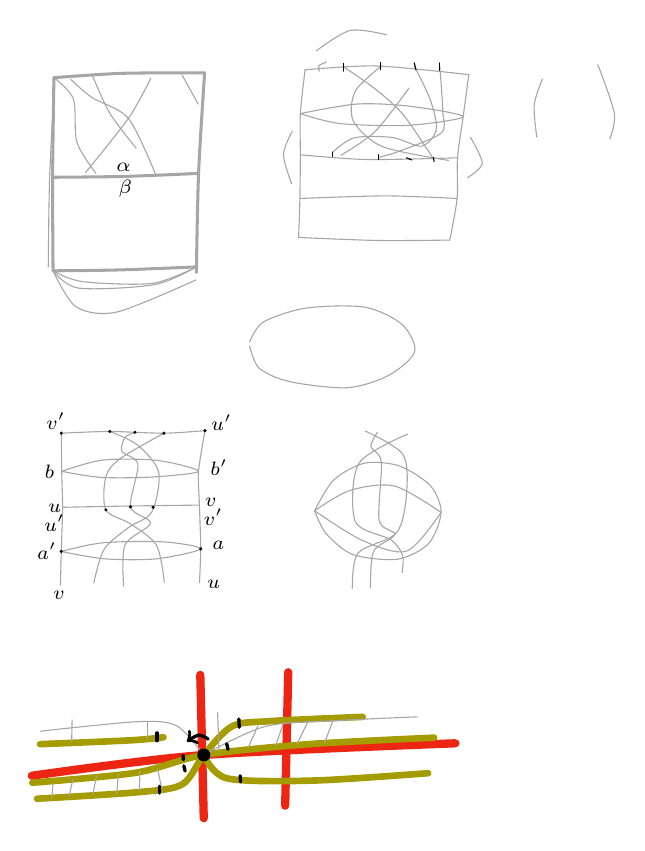
\begin{tikzpicture}[x=.55cm,y=-.55cm,line cap=round,line join=round,g/.style={olive!80!yellow,line width=1.7pt},r/.style={orange!80!brown,line width=1.8pt},w/.style={red!60!black,line width=1.5pt},b/.style={blue!60!black,line width=1.4pt},p/.style={gray!70,thin},k/.style={black,line width=1.2pt},every node/.style={font=\scriptsize}]
\draw[p,line width=1.1pt] plot[smooth] coordinates {(2.71,2.67) (4.29,2.57) (6.19,2.56)};
\draw[p,line width=1.1pt] plot[smooth] coordinates {(2.71,2.67) (2.68,4.97) (2.69,7.13)};
\draw[p,line width=1.1pt] plot[smooth] coordinates {(6.19,2.56) (6.05,4.88) (6.0,7.17)};
\draw[p,line width=1.1pt] plot[smooth] coordinates {(2.68,4.97) (4.36,4.95) (6.05,4.88)};
\draw[p,line width=1.1pt] plot[smooth] coordinates {(2.69,7.13) (4.2,7.11) (6.0,7.04)};
\draw[p] plot[smooth] coordinates {(2.71,2.67) (3.16,3.16) (3.24,4.16) (3.68,4.88)};
\draw[p] plot[smooth] coordinates {(3.1,2.71) (3.59,3.13) (4.43,3.61) (5.06,4.91)};
\draw[p] plot[smooth] coordinates {(3.59,2.6) (4.0,3.49) (4.61,4.3)};
\draw[p] plot[smooth] coordinates {(4.95,2.68) (4.43,3.61) (3.44,4.86)};
\draw[p] plot[smooth] coordinates {(5.67,2.61) (6.04,3.28)};
\draw[p] plot[smooth] coordinates {(2.69,7.13) (3.37,7.38) (4.98,7.42) (6.0,7.04)};
\draw[p] plot[smooth] coordinates {(2.69,7.13) (3.28,7.53) (5.03,7.45) (6.0,7.04)};
\draw[p] plot[smooth] coordinates {(2.69,7.13) (3.22,7.96) (4.17,8.08) (5.99,7.34)};
\draw[p] plot[smooth] coordinates {(2.72,2.8) (2.61,5.0) (2.58,7.04)};
\node at (4.32,4.74) {$\alpha$};
\node at (4.36,5.24) {$\beta$};
\draw[p] plot[smooth] coordinates {(8.51,2.49) (10.15,2.4) (12.29,2.6)};
\draw[p] plot[smooth] coordinates {(8.51,2.49) (8.4,3.5) (8.4,4.45) (8.39,5.46) (8.36,6.36)};
\draw[p] plot[smooth] coordinates {(12.29,2.6) (12.16,3.57) (12.03,4.52) (12.02,5.46) (11.85,6.42)};
\draw[p] plot[smooth] coordinates {(8.4,3.5) (9.7,3.28) (10.93,3.33) (12.16,3.57) (10.9,3.77) (9.32,3.73) (8.4,3.5)};
\draw[p] plot[smooth] coordinates {(8.4,4.45) (9.93,4.56) (12.03,4.52)};
\draw[p] plot[smooth] coordinates {(8.39,5.46) (10.37,5.4) (12.02,5.46)};
\draw[p] plot[smooth] coordinates {(8.36,6.36) (10.2,6.43) (11.85,6.42)};
\draw[p] plot[smooth] coordinates {(8.21,3.91) (8.01,4.45) (8.2,5.12)};
\draw[p] plot[smooth] coordinates {(12.33,4.05) (12.6,4.65) (12.26,4.98)};
\draw[p] plot[smooth] coordinates {(8.84,2.52) (8.83,2.39) (9.01,2.31)};
\draw[p] plot[smooth] coordinates {(9.4,2.42) (10.14,2.94) (10.78,3.53) (11.47,4.54)};
\draw[p] plot[smooth] coordinates {(10.26,2.41) (9.67,2.98) (9.62,3.66) (10.29,4.26) (11.82,4.58)};
\draw[p] plot[smooth] coordinates {(11.03,2.4) (11.4,3.18) (11.54,3.87) (11.2,4.25) (10.52,4.05) (9.64,4.06) (9.15,4.39)};
\draw[p] plot[smooth] coordinates {(11.62,2.4) (11.69,3.45) (11.65,3.95) (10.68,4.37) (10.21,4.51)};
\draw[p] plot[smooth] coordinates {(9.34,4.46) (10.13,3.91) (10.91,2.91)};
\draw[p] plot[smooth] coordinates {(13.99,2.7) (13.8,3.3) (13.86,4.04)};
\draw[p] plot[smooth] coordinates {(15.27,2.37) (15.65,3.49) (15.55,4.08)};
\draw[p] plot[smooth] coordinates {(8.77,2.05) (9.55,1.58) (10.39,1.68)};
\draw[k,thin] plot[smooth] coordinates {(9.4,2.34) (9.4,2.52)};
\draw[k,thin] plot[smooth] coordinates {(10.26,2.32) (10.26,2.49)};
\draw[k,thin] plot[smooth] coordinates {(11.03,2.33) (11.07,2.49)};
\draw[k,thin] plot[smooth] coordinates {(11.62,2.33) (11.62,2.5)};
\draw[k,thin] plot[smooth] coordinates {(9.15,4.39) (9.15,4.49)};
\draw[k,thin] plot[smooth] coordinates {(10.21,4.45) (10.21,4.56)};
\draw[k,thin] plot[smooth] coordinates {(10.85,4.52) (10.97,4.57)};
\draw[k,thin] plot[smooth] coordinates {(11.47,4.51) (11.49,4.61)};
\draw[p] plot[smooth] coordinates {(7.23,8.77) (7.55,8.31) (8.54,7.99) (9.89,7.97) (10.75,8.37) (11.04,9.0) (10.43,9.55) (9.48,9.83) (8.16,9.69) (7.45,9.38) (7.23,8.87)};
\draw[p] plot[smooth] coordinates {(2.88,10.88) (4.0,10.84) (5.25,10.88) (6.2,10.82)};
\draw[p] plot[smooth] coordinates {(2.88,10.88) (2.89,11.76) (2.91,12.59) (2.88,13.61) (2.86,14.39)};
\draw[p] plot[smooth] coordinates {(6.2,10.82) (6.05,11.76) (6.07,12.54) (6.1,13.55) (6.07,14.33)};
\draw[p] plot[smooth] coordinates {(2.89,11.76) (3.84,11.5) (5.11,11.51) (6.05,11.76) (5.0,11.89) (3.8,11.9) (2.89,11.76)};
\draw[p] plot[smooth] coordinates {(2.91,12.59) (4.5,12.56) (6.07,12.54)};
\draw[p] plot[smooth] coordinates {(2.88,13.61) (3.84,13.41) (5.25,13.39) (6.1,13.55) (5.08,13.78) (3.88,13.78) (2.88,13.61)};
\draw[p] plot[smooth] coordinates {(3.63,14.34) (3.87,13.56) (4.43,13.06) (4.97,12.7) (5.13,11.78) (4.64,11.15) (4.0,10.84)};
\draw[p] plot[smooth] coordinates {(4.32,14.41) (4.35,13.46) (4.94,12.96) (4.48,12.58) (4.65,11.6) (4.28,11.3) (4.35,10.98) (4.58,10.86)};
\draw[p] plot[smooth] coordinates {(5.26,14.32) (5.08,13.47) (4.49,12.98) (3.91,12.65) (3.91,11.88) (4.25,11.46) (5.25,10.88)};
\fill[k] (2.88,10.88) circle (.04);
\fill[k] (4.0,10.84) circle (.04);
\fill[k] (4.58,10.86) circle (.04);
\fill[k] (5.25,10.88) circle (.04);
\fill[k] (6.2,10.82) circle (.04);
\fill[k] (3.91,12.65) circle (.04);
\fill[k] (4.48,12.58) circle (.04);
\fill[k] (5.0,12.59) circle (.04);
\fill[k] (2.88,13.61) circle (.04);
\fill[k] (6.1,13.55) circle (.04);
\node at (2.75,10.6) {$v'$};
\node at (6.58,10.64) {$u'$};
\node at (2.61,11.78) {$\unsure{b}$};
\node at (6.52,11.68) {$b'$};
\node at (2.73,12.61) {$\unsure{u}$};
\node at (2.72,12.96) {$\unsure{u'}$};
\node at (6.33,12.47) {$\unsure{v}$};
\node at (6.39,12.82) {$\unsure{v'}$};
\node at (2.55,13.6) {$a'$};
\node at (6.51,13.48) {$a$};
\node at (2.83,14.63) {$\unsure{v}$};
\node at (6.4,14.38) {$u$};
\draw[p] plot[smooth] coordinates {(8.73,12.67) (9.17,11.96) (9.89,11.57) (10.7,11.64) (11.41,12.1) (11.65,12.71) (11.36,13.43) (10.64,13.79) (9.61,13.68) (8.99,13.19) (8.73,12.67)};
\draw[p] plot[smooth] coordinates {(8.73,12.67) (9.55,12.2) (10.58,12.1) (11.65,12.71)};
\draw[p] plot[smooth] coordinates {(8.73,12.67) (9.82,13.35) (10.86,13.6) (11.65,12.71)};
\draw[p] plot[smooth] coordinates {(9.9,10.83) (10.77,11.37) (10.85,12.31) (10.62,13.18) (9.73,13.65) (9.6,14.46)};
\draw[p] plot[smooth] coordinates {(10.88,10.9) (9.75,11.58) (9.67,12.92) (10.49,13.34) (10.76,13.7) (10.75,14.1)};
\draw[p] plot[smooth] coordinates {(10.18,10.86) (10.03,11.19) (10.27,11.54) (10.22,12.89) (10.58,13.22) (10.09,13.61) (10.02,14.45)};
\draw[red!70!brown,line width=3pt] plot[smooth] coordinates {(6.09,16.46) (6.17,19.77)};
\draw[red!70!brown,line width=3pt] plot[smooth] coordinates {(8.12,16.4) (8.05,19.48)};
\draw[red!70!brown,line width=3pt] plot[smooth] coordinates {(2.2,18.79) (6.17,18.31) (11.98,18.04)};
\draw[g,line width=2.4pt] plot[smooth] coordinates {(2.39,18.06) (4.5,17.97) (5.24,17.9)};
\draw[g,line width=2.4pt] plot[smooth] coordinates {(2.32,19.32) (4.64,19.17) (5.67,18.99) (6.17,18.31) (6.82,17.65) (7.67,17.53) (9.84,17.43)};
\draw[g,line width=2.4pt] plot[smooth] coordinates {(2.21,18.95) (4.6,18.72) (6.17,18.31) (8.59,18.06) (11.49,17.91)};
\draw[g,line width=2.4pt] plot[smooth] coordinates {(6.17,18.31) (6.71,18.85) (8.71,18.9) (11.35,18.73)};
\draw[p] plot[smooth] coordinates {(2.4,17.76) (4.66,17.54) (5.55,17.64) (6.17,18.31)};
\draw[p] plot[smooth] coordinates {(6.17,18.31) (7.59,17.65) (9.34,17.51) (11.1,17.43)};
\draw[p] plot[smooth] coordinates {(2.69,18.97) (2.66,19.3)};
\draw[p] plot[smooth] coordinates {(3.15,18.86) (3.06,19.27)};
\draw[p] plot[smooth] coordinates {(3.69,18.8) (3.61,19.22)};
\draw[p] plot[smooth] coordinates {(4.2,18.75) (4.16,19.19)};
\draw[p] plot[smooth] coordinates {(4.7,18.68) (4.68,19.13)};
\draw[p] plot[smooth] coordinates {(5.1,18.62) (5.2,19.08)};
\draw[p] plot[smooth] coordinates {(3.13,17.5) (3.12,17.99)};
\draw[p] plot[smooth] coordinates {(4.88,17.56) (4.88,17.94)};
\draw[p] plot[smooth] coordinates {(6.49,17.32) (6.52,18.17)};
\draw[p] plot[smooth] coordinates {(7.42,17.64) (7.2,18.13)};
\draw[p] plot[smooth] coordinates {(8.01,17.57) (7.83,18.09)};
\draw[p] plot[smooth] coordinates {(8.57,17.55) (8.32,18.06)};
\draw[p] plot[smooth] coordinates {(9.16,17.5) (8.96,18.03)};
\draw[k] plot[smooth] coordinates {(5.09,17.8) (5.09,17.98)};
\draw[k] plot[smooth] coordinates {(5.15,19.03) (5.15,19.19)};
\draw[k] plot[smooth] coordinates {(6.98,17.48) (6.99,17.67)};
\draw[k] plot[smooth] coordinates {(7.01,18.79) (7.02,18.93)};
\draw[k] plot[smooth] coordinates {(6.7,18.05) (6.73,18.18)};
\draw[k] plot[smooth] coordinates {(5.69,18.32) (5.7,18.42)};
\draw[k] plot[smooth] coordinates {(5.71,18.56) (5.74,18.68)};
\draw[k,->] plot[smooth] coordinates {(6.27,17.94) (6.05,17.85) (5.78,18.0)};
\fill[k] (6.17,18.31) circle (.15);
\end{tikzpicture}}
{\scriptsize\ttfamily\begin{tabular}{l}
******************************************************************\\
* *\\
* - J E S N E W S F R 1 - LE 06/08/82 *\\
* *\\
*----------------------------------------------------------------*\\
* *\\
* DEPUIS LE LUNDI 12 JUILLET 82, LES CLASSES DE TRAVAUX D ET E *\\
* SERONT ETENDUES POUR UNE TAILLE MEMOIRE SUPERIEURE A 1024 K *\\
* SE REPORTER A LA NOTE TECHNIQUE MVS141. *\\
* *\\
*----------------------------------------------------------------*\\
* A PARTIR DU LUNDI 9 AOUT 1982 , IL SERA POSSIBLE D'IMPRIMER *\\
* SUR XEROX 9700 (DESTINATION SAC) DES FICHIERS UTILISANT LE *\\
* COUPLE DE JEUX DE CARACTERES : (GS15,GT15) *\\
******************************************************************\\
\end{tabular}}
{\scriptsize\ttfamily\begin{tabular}{l}
********************************************************************************\\
*JESNEWS DU 09/08/1982 C68 CADARACHE *\\
********************************************************************************\\
* DEPUIS LE 1/7/82 LES ALIAS DES COMMANDES LIBRARIAN *\\
* LIBGET (LG) ET LIBSAVE (LS) SONT SUPPRIMES, *\\
* POUR EVITER UNE POSSIBILITE DE CONFLIT AVEC *\\
* LE MEME ALIAS DES COMMANDES STANDARD IBM. *\\
* ******* *\\
* ATTENTION *\\
* MISE EN SERVICE LE VENDREDI 30/7/82 A 8H00 DE LA DEUXIEME PHASE DE GAF *\\
* SUR 168 CADARACHE. *\\
* ELLE PERMET D'UTILISER DANS LA CDE. KEEP TSO ET DANS LA PROCEDURE KEEP *\\
* BATCH UNE POSSIBILITE D'AFFECTATION DE TYPE DE SAUVEGARDE AU NIVEAU DU *\\
* FICHIER.CETTE POSSIBILITE EST VIVEMENT CONSEILLEE. *\\
* POUR PLUS AMPLES INFORMATIONS VOIR NOTE TECHNIQUE CISI MVS140,LA NOTE *\\
* MVS 143 ETANT SUPPRIMEE. *\\
* *\\
* EXEMPLES D'UTILISATION: *\\
* *\\
* BATCH: DSN=NOM.DU.FICHIER.A.SAUVEGARDER,DELAY=TYPE DE SAUVEGARDE *\\
* *\\
* TSO: *\\
* K DA('NOM DU FICHIER A SAUVEGARDER') DELAY(TYPE DE SAUVEGARDE) *\\
* *\\
* TYPES DE SAUVEGARDE: *\\
* *\\
* W SAUVEGARDE HEBDO. *\\
* D SAUVEGARDE JOURNALIERE. *\\
* NOS SAUVEGARDE MENSUELLE. *\\
* W PARAMETRE PAR DEFAUT. *\\
* *\\
********************************************************************************\\
\end{tabular}}
\margin{\mspage{158}}

\scanpage{160}
\deleted{
\uline{1.1.84}

Compléments et rectifications sur les facettes exceptionnelles de $(\unsure{X|\mathcal X},K)$

a) Avec les notations de \unsure{i)}, on a
\[
\varphi^{-1}(\unsure{X_1^a|X_1^0})=L\cup K_0\qquad(\text{et non }=L\,!)
\]

b) La structure d'une facette exceptionnelle au voisinage d'une arête exceptionnelle (ou mieux, de la \inserted{double} paire de facettes rattachées à un sommet exceptionnel $a$) est de la forme suivante :
\figure{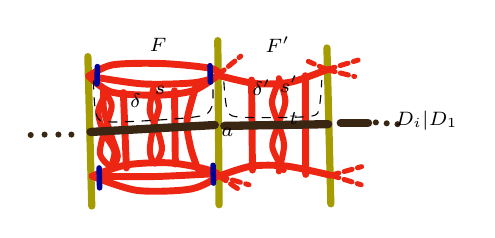
\begin{tikzpicture}[x=.55cm,y=-.55cm,line cap=round,line join=round,g/.style={olive!80!yellow,line width=1.7pt},r/.style={orange!80!brown,line width=1.8pt},w/.style={red!60!black,line width=1.5pt},b/.style={blue!60!black,line width=1.4pt},p/.style={gray!70,thin},k/.style={black,line width=1.2pt},every node/.style={font=\scriptsize}]
\draw[g,line width=2.6pt] plot[smooth] coordinates {(2.98,11.4) (3.07,14.85)};
\draw[g,line width=2.6pt] plot[smooth] coordinates {(5.98,11.03) (6.01,14.82)};
\draw[g,line width=2.6pt] plot[smooth] coordinates {(8.5,11.2) (8.59,14.8)};
\draw[red!70!brown,line width=2.5pt] plot[smooth] coordinates {(3.0,11.85) (3.55,11.59) (4.7,11.56) (5.81,11.67) (5.98,11.83) (5.46,12.0) (4.25,12.03) (3.0,11.85)};
\draw[red!70!brown,line width=2.5pt] plot[smooth] coordinates {(3.0,11.85) (3.53,12.22) (4.62,12.29) (5.43,12.18) (5.98,11.83)};
\draw[red!70!brown,line width=2.5pt] plot[smooth] coordinates {(3.08,14.16) (3.88,13.9) (4.95,13.86) (5.96,14.1) (5.39,14.45) (4.12,14.49) (3.08,14.16)};
\draw[red!70!brown,line width=2.5pt] plot[smooth] coordinates {(3.08,14.16) (4.5,14.17) (5.96,14.1)};
\draw[red!70!brown,line width=2.5pt] plot[smooth] coordinates {(5.98,11.83) (6.84,12.02) (7.66,11.99) (8.5,11.7)};
\draw[red!70!brown,line width=2.5pt] plot[smooth] coordinates {(6.01,14.16) (6.75,13.93) (7.58,13.93) (8.59,14.14)};
\draw[red!70!brown,line width=2.5pt] plot[smooth] coordinates {(3.8,12.23) (3.87,13.97)};
\draw[red!70!brown,line width=2.5pt] plot[smooth] coordinates {(4.98,12.19) (5.0,13.88)};
\draw[red!70!brown,line width=2.5pt] plot[smooth] coordinates {(5.47,12.11) (5.27,12.88) (5.35,13.49) (5.51,13.98)};
\draw[red!70!brown,line width=2.5pt] plot[smooth] coordinates {(6.76,11.94) (6.78,14.02)};
\draw[red!70!brown,line width=2.5pt] plot[smooth] coordinates {(8.0,11.84) (8.01,14.12)};
\draw[red!70!brown,line width=2.2pt] plot[smooth] coordinates {(3.33,12.16) (3.53,12.53) (3.36,13.11) (3.26,13.65) (3.51,13.93) (3.67,13.7) (3.51,13.19) (3.36,12.69) (3.33,12.16)};
\draw[red!70!brown,line width=2.2pt] plot[smooth] coordinates {(3.42,12.21) (3.22,12.65) (3.33,13.12) (3.59,13.58) (3.51,13.95)};
\draw[red!70!brown,line width=2.2pt] plot[smooth] coordinates {(4.49,12.15) (4.62,12.55) (4.49,13.02) (4.41,13.58) (4.53,13.87) (4.69,13.55) (4.6,13.13) (4.41,12.66) (4.49,12.15)};
\draw[red!70!brown,line width=2.2pt] plot[smooth] coordinates {(7.39,11.9) (7.54,12.43) (7.37,12.98) (7.24,13.49) (7.5,14.02)};
\draw[red!70!brown,line width=2.2pt] plot[smooth] coordinates {(7.4,11.95) (7.23,12.45) (7.39,12.98) (7.51,13.45) (7.39,14.05)};
\draw[red!70!brown,densely dashed,line width=1.8pt] plot[smooth] coordinates {(5.98,11.83) (6.51,11.39)};
\draw[red!70!brown,densely dashed,line width=1.8pt] plot[smooth] coordinates {(8.5,11.7) (8.07,11.51)};
\draw[red!70!brown,densely dashed,line width=1.8pt] plot[smooth] coordinates {(8.5,11.7) (9.22,11.48)};
\draw[red!70!brown,densely dashed,line width=1.8pt] plot[smooth] coordinates {(8.5,11.7) (9.14,11.86)};
\draw[red!70!brown,densely dashed,line width=1.8pt] plot[smooth] coordinates {(6.01,14.16) (6.7,14.36)};
\draw[red!70!brown,densely dashed,line width=1.8pt] plot[smooth] coordinates {(6.01,14.16) (6.44,14.45)};
\draw[red!70!brown,densely dashed,line width=1.8pt] plot[smooth] coordinates {(8.59,14.14) (9.3,13.94)};
\draw[red!70!brown,densely dashed,line width=1.8pt] plot[smooth] coordinates {(8.59,14.14) (9.29,14.36)};
\draw[k,dashed,thin] plot[smooth] coordinates {(3.11,11.96) (3.18,12.75) (3.55,12.91) (5.47,12.79) (5.84,12.56) (5.86,11.94)};
\draw[k,dashed,thin] plot[smooth] coordinates {(6.12,11.98) (6.21,12.66) (6.55,12.8) (8.1,12.78) (8.32,12.57) (8.38,11.95)};
\draw[black!70!brown,line width=3pt] plot[smooth] coordinates {(3.04,13.14) (5.91,12.98)};
\draw[black!70!brown,line width=3pt] plot[smooth] coordinates {(6.13,13.0) (8.53,12.96)};
\draw[black!70!brown,line width=3pt] plot[smooth] coordinates {(8.82,12.93) (9.45,12.93)};
\fill[black!70!brown] (1.66,13.21) circle (.07);
\fill[black!70!brown] (1.98,13.2) circle (.07);
\fill[black!70!brown] (2.3,13.2) circle (.07);
\fill[black!70!brown] (2.6,13.2) circle (.07);
\fill[black!70!brown] (9.63,12.92) circle (.07);
\fill[black!70!brown] (9.88,12.94) circle (.07);
\fill[black!70!brown] (10.13,12.96) circle (.07);
\draw[blue!60!black,line width=2pt] plot[smooth] coordinates {(3.2,11.63) (3.19,12.03)};
\draw[blue!60!black,line width=2pt] plot[smooth] coordinates {(5.8,11.61) (5.81,11.99)};
\draw[blue!60!black,line width=2pt] plot[smooth] coordinates {(3.24,13.97) (3.25,14.43)};
\draw[blue!60!black,line width=2pt] plot[smooth] coordinates {(5.87,13.91) (5.88,14.32)};
\node at (4.6,11.13) {$F$};
\node at (7.36,11.13) {$F'$};
\node at (4.08,12.43) {$\delta$};
\node at (6.99,12.12) {$\delta'$};
\node at (4.65,12.17) {$\unsure{s}$};
\node at (7.62,12.04) {$\unsure{s'}$};
\node at (10.8,12.87) {$\unsure{D_i|D_1}$};
\node at (6.2,13.14) {$\unsure{a}$};
\node at (7.73,12.84) {$\unsure{t}$};
\end{tikzpicture}}

Choix d'une \unsure{la} ``branche principale'' \inserted{$\delta$} de $L$ dans une face exceptionnelle ($F$ ou $F'$ disons) en un sommet \deleted{multiple}\inserted{multiple $s$}; alors les branches de $L$ en $s$ distinctes de \deleted{$\unsure{\delta}$} $\delta$ sont concourantes en un m\textsuperscript{me} pt $\unsure{t}$ de $\partial F$ sur $K_0$ (et par la loi de symétrie, le m\textsuperscript{me} doit se faire avec m\textsuperscript{me} multiplicité.

(De plus, je rappelle que la loi de symétrie s'étend à la multiplicité des \unsure{pts demi sommets|pts deux sommets} \deleted{\unsure{multiples}} \inserted{de $L$} qui se trouvent sur les deux arêtes ordinaires, incidentes à $a$.)

c) Pour les arêtes de $F$ \inserted{\unsure{non exceptionnelles en $F$}} distinctes des trois arêtes marquées, \deleted{\unsure{la}} la \deleted{bord} rive privilégiée est celle opposée à cette face. -- pour une arête \inserted{ordinaire} passant par un sommet exceptionnel (arête marquée en vert), la \deleted{arête}\inserted{rive} privilégiée est celle qui correspond à la face \unsure{instble}.

d) Pour avoir la position relative correspondant à une face exceptionnelle, il faut modifier le \unsure{ruban généralisé} \deleted{\unsure{(disons}} (dis. $A$ qui \unsure{prend} $\varphi(\partial F^*)$, où $F^*$ est déduite de $F$ par renflement \unsure{en} les sommets critiques dans la rive \deleted{\unsure{exceptionelle}} privilégiée et opposée à $F$) en \deleted{\unsure{faisant une}}\inserted{déformant $F^*$ de} façon similaire, à partir de la modification obtenue en remplaçant ``\uuline{l'arc} \deleted{\unsure{des deux pts exceptionnels de}} \inserted{\unsure{du bord}} exceptionnel'' \deleted{de la}\inserted{de la} face envisagée (joignant les deux pts critiques principaux \deleted{sur la} face) par un ``\unsure{path}'' parallèle à l'intérieur de $F$ (cf. pointillé au stylo).
}
\margin{\mspage{159}}

\scanpage{161}
\figure{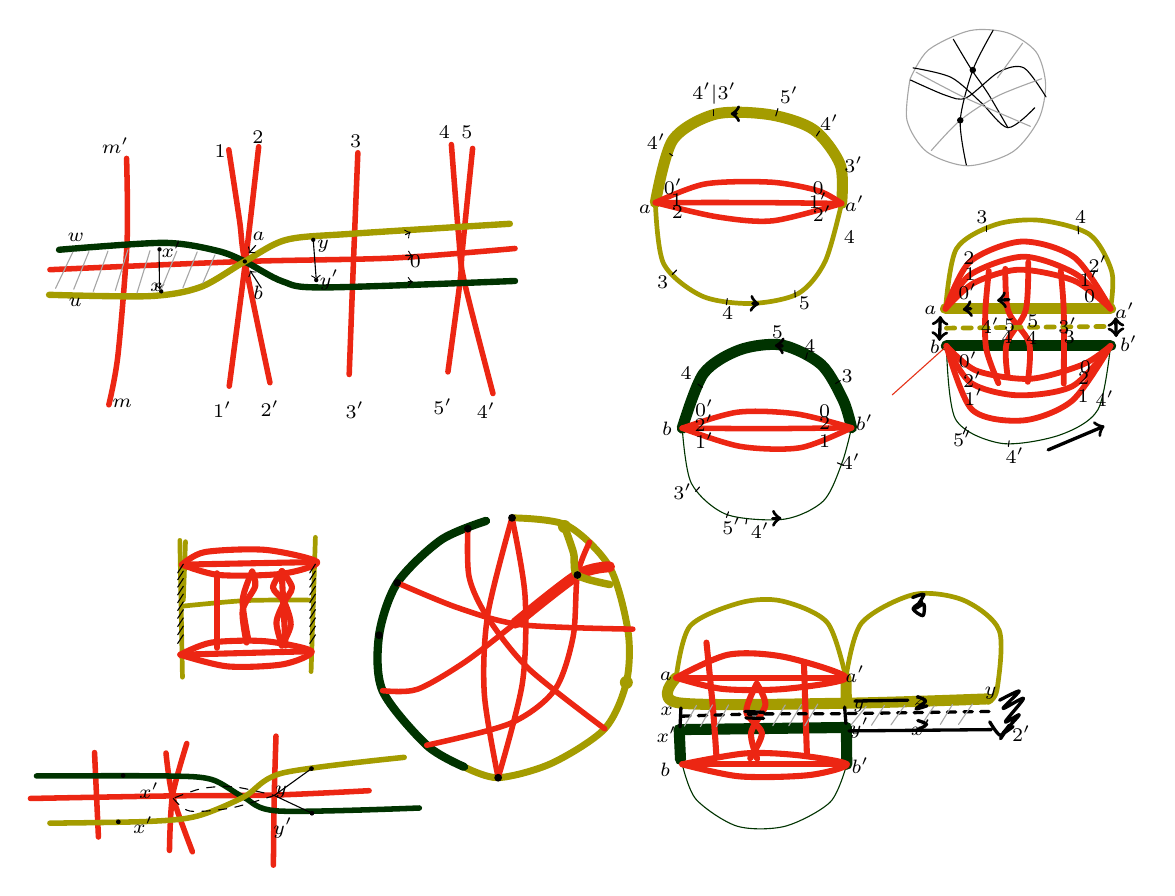
\begin{tikzpicture}[x=.55cm,y=-.55cm,line cap=round,line join=round,g/.style={olive!80!yellow,line width=1.7pt},r/.style={orange!80!brown,line width=1.8pt},w/.style={red!60!black,line width=1.5pt},b/.style={blue!60!black,line width=1.4pt},p/.style={gray!70,thin},k/.style={black,line width=1.2pt},every node/.style={font=\scriptsize}]
\draw[red!70!brown,line width=2pt] plot[smooth] coordinates {(3.94,4.65) (3.95,6.6) (3.74,9.2) (3.53,10.34)};
\draw[red!70!brown,line width=2pt] plot[smooth] coordinates {(6.3,4.45) (6.55,6.1) (6.67,7.03) (7.25,9.83)};
\draw[red!70!brown,line width=2pt] plot[smooth] coordinates {(6.99,4.38) (6.69,6.99) (6.31,9.91)};
\draw[red!70!brown,line width=2pt] plot[smooth] coordinates {(9.28,4.52) (9.18,7.0) (9.08,9.64)};
\draw[red!70!brown,line width=2pt] plot[smooth] coordinates {(11.44,4.33) (11.61,6.47) (11.73,7.46) (12.4,10.08)};
\draw[red!70!brown,line width=2pt] plot[smooth] coordinates {(11.93,4.42) (11.69,6.8) (11.64,7.49) (11.36,9.58)};
\draw[red!70!brown,line width=2pt] plot[smooth] coordinates {(2.17,7.22) (6.67,7.03) (10.1,6.95) (12.91,6.73)};
\draw[green!20!black,line width=2.3pt] plot[smooth] coordinates {(2.38,6.76) (4.79,6.6) (6.02,6.78) (6.67,7.03) (7.54,7.49) (8.49,7.63) (12.91,7.48)};
\draw[g,line width=2.3pt] plot[smooth] coordinates {(2.15,7.8) (4.48,7.83) (5.65,7.62) (6.67,7.03) (7.63,6.53) (9.14,6.39) (12.79,6.16)};
\draw[k,thin,->] plot[smooth] coordinates {(4.69,6.76) (4.7,7.67)};
\draw[k,thin,->] plot[smooth] coordinates {(8.25,6.53) (8.32,7.46)};
\draw[k,thin,->] plot[smooth] coordinates {(10.38,6.41) (10.5,6.35)};
\draw[k,thin,->] plot[smooth] coordinates {(10.38,6.89) (10.55,6.9)};
\draw[k,thin,->] plot[smooth] coordinates {(10.44,7.5) (10.55,7.5)};
\draw[k,thin,->] plot[smooth] coordinates {(6.92,6.66) (6.76,6.84)};
\draw[k,thin,->] plot[smooth] coordinates {(7.05,7.64) (6.79,7.24)};
\draw[p] plot[smooth] coordinates {(2.3,7.65) (2.7,6.81)};
\draw[p] plot[smooth] coordinates {(2.72,7.67) (3.07,6.8)};
\draw[p] plot[smooth] coordinates {(3.17,7.72) (3.51,6.79)};
\draw[p] plot[smooth] coordinates {(3.68,7.7) (3.97,6.76)};
\draw[p] plot[smooth] coordinates {(4.18,7.76) (4.48,6.78)};
\draw[p] plot[smooth] coordinates {(4.75,7.65) (5.1,6.79)};
\draw[p] plot[smooth] coordinates {(5.24,7.64) (5.57,6.81)};
\draw[p] plot[smooth] coordinates {(5.7,7.53) (5.98,6.88)};
\fill[k] (4.7,6.75) circle (.05);
\fill[k] (4.74,7.72) circle (.05);
\fill[k] (8.25,6.53) circle (.05);
\fill[k] (8.32,7.46) circle (.05);
\fill[k] (6.67,7.03) circle (.05);
\node at (3.68,4.36) {$\unsure{m'}$};
\node at (3.84,10.31) {$\unsure{m}$};
\node at (6.1,4.48) {$1$};
\node at (6.97,4.17) {$2$};
\node at (9.23,4.26) {$3$};
\node at (11.28,4.04) {$4$};
\node at (11.8,4.04) {$5$};
\node at (6.15,10.45) {$1'$};
\node at (7.25,10.43) {$2'$};
\node at (9.21,10.46) {$3'$};
\node at (11.24,10.38) {$5'$};
\node at (12.24,10.47) {$4'$};
\node at (2.77,6.48) {$\unsure{w}$};
\node at (2.75,7.98) {$u$};
\node at (4.98,6.75) {$x'$};
\node at (4.63,7.63) {$x$};
\node at (8.48,6.67) {$y$};
\node at (8.62,7.46) {$y'$};
\node at (6.99,6.45) {$a$};
\node at (6.98,7.75) {$\unsure{b}$};
\node at (10.61,7.02) {$0$};
\draw[p] plot[smooth] coordinates {(22.03,2.82) (22.45,2.15) (23.41,1.7) (24.28,1.75) (24.94,2.19) (25.16,2.93) (25.0,3.75) (24.4,4.5) (23.36,4.82) (22.42,4.5) (21.96,3.77) (22.03,2.82)};
\draw[k,thin] plot[smooth] coordinates {(22.1,2.56) (22.98,2.78) (23.67,3.36) (24.29,3.94) (24.91,3.48)};
\draw[k,thin] plot[smooth] coordinates {(22.04,2.84) (22.87,3.2) (23.33,3.25) (24.09,2.65) (24.66,2.56) (25.17,3.23)};
\draw[k,thin] plot[smooth] coordinates {(23.03,1.9) (23.45,2.6) (23.83,3.15) (24.29,3.94)};
\draw[k,thin] plot[smooth] coordinates {(23.95,1.69) (23.48,2.61) (23.19,3.77) (23.33,4.8)};
\draw[p] plot[smooth] coordinates {(22.52,4.47) (23.19,3.77) (24.05,3.21) (25.07,2.81)};
\draw[p] plot[smooth] coordinates {(22.17,2.66) (23.3,3.25) (24.81,3.91)};
\draw[p] plot[smooth] coordinates {(24.63,1.99) (24.05,2.79)};
\fill[k] (23.48,2.61) circle (.075);
\fill[k] (23.19,3.77) circle (.075);
\draw[g,line width=4pt] plot[smooth] coordinates {(16.15,5.67) (16.55,4.23) (17.53,3.63) (18.79,3.64) (19.81,3.99) (20.42,4.8) (20.45,5.69)};
\draw[g] plot[smooth] coordinates {(16.15,5.67) (16.34,7.08) (17.23,7.83) (18.37,8.0) (19.45,7.77) (20.07,7.03) (20.45,5.69)};
\draw[red!70!brown,line width=2pt] plot[smooth] coordinates {(16.15,5.67) (17.3,5.24) (18.83,5.2) (19.92,5.4) (20.45,5.69)};
\draw[red!70!brown,line width=2pt] plot[smooth] coordinates {(16.15,5.67) (18.4,5.67) (20.45,5.69)};
\draw[red!70!brown,line width=2pt] plot[smooth] coordinates {(16.15,5.67) (17.58,6.0) (18.87,6.09) (20.45,5.69)};
\draw[k,->] plot[smooth] coordinates {(18.02,3.62) (17.89,3.62)};
\draw[k,->] plot[smooth] coordinates {(18.4,8.0) (18.55,8.01)};
\draw[k,thin] plot[smooth] coordinates {(17.49,3.66) (17.49,3.53)};
\draw[k,thin] plot[smooth] coordinates {(18.93,3.67) (18.98,3.5)};
\draw[k,thin] plot[smooth] coordinates {(19.87,4.13) (19.94,4.02)};
\draw[k,thin] plot[smooth] coordinates {(16.48,4.54) (16.55,4.59)};
\draw[k,thin] plot[smooth] coordinates {(16.64,7.23) (16.54,7.33)};
\draw[k,thin] plot[smooth] coordinates {(17.81,7.89) (17.79,8.03)};
\draw[k,thin] plot[smooth] coordinates {(19.37,7.7) (19.38,7.85)};
\node at (15.91,5.83) {$a$};
\node at (20.75,5.69) {$a'$};
\node at (16.56,5.3) {$0'$};
\node at (16.64,5.62) {$1$};
\node at (16.66,5.9) {$2$};
\node at (19.91,5.33) {$\unsure{0}$};
\node at (19.91,5.62) {$1'$};
\node at (20.0,5.93) {$2'$};
\node at (17.51,3.15) {$\unsure{4'|3'}$};
\node at (19.24,3.19) {$5'$};
\node at (20.17,3.82) {$4'$};
\node at (20.73,4.79) {$3'$};
\node at (16.17,4.26) {$\unsure{4'}$};
\node at (20.63,6.46) {$4$};
\node at (16.32,7.52) {$3$};
\node at (17.82,8.22) {$4$};
\node at (19.59,7.99) {$5$};
\draw[green!20!black,line width=4pt] plot[smooth] coordinates {(16.77,10.88) (17.26,9.62) (18.1,9.07) (19.07,8.96) (19.98,9.41) (20.49,10.24) (20.68,10.87)};
\draw[green!20!black] plot[smooth] coordinates {(16.77,10.88) (16.98,12.15) (17.79,12.87) (19.13,12.98) (20.03,12.56) (20.46,11.68) (20.68,10.87)};
\draw[red!70!brown,line width=2pt] plot[smooth] coordinates {(16.77,10.88) (18.05,10.51) (19.41,10.55) (20.68,10.87)};
\draw[red!70!brown,line width=2pt] plot[smooth] coordinates {(16.77,10.88) (18.81,10.89) (20.68,10.87)};
\draw[red!70!brown,line width=2pt] plot[smooth] coordinates {(16.77,10.88) (18.11,11.3) (19.5,11.33) (20.68,10.87)};
\draw[k,->] plot[smooth] coordinates {(19.08,8.98) (18.91,8.97)};
\draw[k,->] plot[smooth] coordinates {(18.86,12.96) (19.06,12.96)};
\draw[k,thin] plot[smooth] coordinates {(17.13,9.86) (17.23,9.94)};
\draw[k,thin] plot[smooth] coordinates {(19.62,9.28) (19.66,9.14)};
\draw[k,thin] plot[smooth] coordinates {(20.31,9.85) (20.42,9.78)};
\draw[k,thin] plot[smooth] coordinates {(17.17,12.24) (17.08,12.34)};
\draw[k,thin] plot[smooth] coordinates {(17.84,12.81) (17.79,12.94)};
\draw[k,thin] plot[smooth] coordinates {(18.26,12.98) (18.24,13.09)};
\draw[k,thin] plot[smooth] coordinates {(20.35,11.68) (20.5,11.74)};
\node at (16.42,10.9) {$b$};
\node at (20.98,10.75) {$b'$};
\node at (17.28,10.42) {$0'$};
\node at (17.27,10.76) {$2'$};
\node at (17.28,11.17) {$1'$};
\node at (20.06,10.48) {$0$};
\node at (20.06,10.77) {$2$};
\node at (20.06,11.18) {$1$};
\node at (16.86,9.62) {$4$};
\node at (18.97,8.66) {$5$};
\node at (19.72,8.99) {$\unsure{4}$};
\node at (20.58,9.67) {$3$};
\node at (20.67,11.65) {$4'$};
\node at (16.78,12.35) {$3'$};
\node at (17.91,13.14) {$5'$};
\node at (18.57,13.25) {$4'$};
\draw[g] plot[smooth] coordinates {(22.85,8.12) (23.1,6.74) (24.0,6.18) (25.04,6.08) (26.18,6.41) (26.69,7.27) (26.66,8.12)};
\draw[green!20!black] plot[smooth] coordinates {(22.87,8.98) (23.08,10.67) (24.14,11.23) (25.48,11.04) (26.37,10.45) (26.66,8.98)};
\draw[g,line width=4pt] plot[smooth] coordinates {(22.85,8.12) (26.66,8.12)};
\draw[green!20!black,line width=4pt] plot[smooth] coordinates {(22.87,8.98) (26.66,8.98)};
\draw[red!70!brown,line width=2.1pt] plot[smooth] coordinates {(22.85,8.12) (23.41,7.04) (24.61,6.57) (25.83,6.94) (26.66,8.12)};
\draw[red!70!brown,line width=2.1pt] plot[smooth] coordinates {(22.85,8.12) (23.43,7.33) (24.65,6.92) (25.86,7.32) (26.66,8.12)};
\draw[red!70!brown,line width=2.1pt] plot[smooth] coordinates {(22.85,8.12) (23.5,7.53) (24.55,7.22) (25.83,7.48) (26.66,8.12)};
\draw[red!70!brown,line width=2.1pt] plot[smooth] coordinates {(22.87,8.98) (23.56,9.55) (24.8,9.74) (26.02,9.41) (26.66,8.98)};
\draw[red!70!brown,line width=2.1pt] plot[smooth] coordinates {(22.87,8.98) (23.43,9.83) (24.51,10.12) (25.78,9.91) (26.66,8.98)};
\draw[red!70!brown,line width=2.1pt] plot[smooth] coordinates {(22.87,8.98) (23.46,10.45) (24.65,10.7) (25.78,10.24) (26.66,8.98)};
\draw[red!70!brown,line width=2.1pt] plot[smooth] coordinates {(23.85,7.25) (23.77,8.17) (23.79,9.05) (24.07,9.84)};
\draw[red!70!brown,line width=2.1pt] plot[smooth] coordinates {(24.23,7.2) (24.3,8.18) (24.78,8.91) (24.75,9.81)};
\draw[red!70!brown,line width=2.1pt] plot[smooth] coordinates {(24.76,7.05) (24.7,8.16) (24.26,8.92) (24.28,9.65)};
\draw[red!70!brown,line width=2.1pt] plot[smooth] coordinates {(25.51,7.25) (25.58,8.18) (25.58,9.85)};
\draw[g,dashed] plot[smooth] coordinates {(22.87,8.57) (26.63,8.53)};
\draw[k,->] plot[smooth] coordinates {(23.43,8.12) (23.25,8.14)};
\draw[k,->] plot[smooth] coordinates {(24.31,7.91) (24.04,7.93)};
\draw[k,->] plot[smooth] coordinates {(25.22,11.38) (26.52,10.83)};
\draw[k,<->] plot[smooth] coordinates {(22.73,8.29) (22.71,8.86)};
\draw[k,<->] plot[smooth] coordinates {(26.78,8.32) (26.79,8.77)};
\draw[k,thin] plot[smooth] coordinates {(23.8,6.21) (23.8,6.34)};
\draw[k,thin] plot[smooth] coordinates {(25.91,6.21) (25.92,6.39)};
\draw[k,thin] plot[smooth] coordinates {(23.33,10.85) (23.26,11.01)};
\draw[k,thin] plot[smooth] coordinates {(24.32,11.17) (24.3,11.3)};
\draw[red!60!brown,thin] plot[smooth] coordinates {(22.88,8.98) (21.62,10.11)};
\node at (22.5,8.15) {$a$};
\node at (26.99,8.17) {$a'$};
\node at (22.6,9.01) {$b$};
\node at (27.08,8.93) {$b'$};
\node at (23.39,6.96) {$2$};
\node at (23.42,7.32) {$1$};
\node at (23.36,7.72) {$0'$};
\node at (26.37,7.09) {$2'$};
\node at (26.16,7.43) {$1'$};
\node at (26.18,7.84) {$0$};
\node at (23.37,9.29) {$0'$};
\node at (23.47,9.76) {$2'$};
\node at (23.5,10.16) {$1'$};
\node at (26.08,9.47) {$0$};
\node at (26.04,9.72) {$2$};
\node at (26.03,10.15) {$1$};
\node at (23.69,6.0) {$3$};
\node at (25.97,6.0) {$4$};
\node at (26.53,10.2) {$4'$};
\node at (23.24,11.12) {$5'$};
\node at (24.45,11.51) {$4'$};
\node at (23.88,8.51) {$\unsure{4'}$};
\node at (24.33,8.51) {$\unsure{5}$};
\node at (24.87,8.4) {$\unsure{5}$};
\node at (25.67,8.51) {$3'$};
\node at (25.71,8.78) {$3$};
\node at (24.84,8.8) {$4$};
\node at (24.27,8.78) {$\unsure{4}$};
\draw[g] plot[smooth] coordinates {(5.17,13.47) (5.23,16.63)};
\draw[g] plot[smooth] coordinates {(5.3,13.5) (5.25,14.85)};
\draw[g] plot[smooth] coordinates {(8.3,13.4) (8.2,16.5)};
\draw[g] plot[smooth] coordinates {(5.22,14.99) (6.7,14.86) (8.23,14.85)};
\draw[red!70!brown,line width=2.2pt] plot[smooth] coordinates {(5.22,14.03) (5.75,13.74) (7.15,13.69) (8.34,13.97) (7.54,14.24) (6.08,14.27) (5.22,14.03)};
\draw[red!70!brown,line width=2.2pt] plot[smooth] coordinates {(5.22,14.03) (8.34,13.97)};
\draw[red!70!brown,line width=2.2pt] plot[smooth] coordinates {(5.18,16.11) (5.9,15.83) (7.15,15.8) (8.21,16.03) (7.56,16.33) (6.27,16.38) (5.18,16.11)};
\draw[red!70!brown,line width=2.2pt] plot[smooth] coordinates {(5.18,16.11) (8.21,16.03)};
\draw[red!70!brown,line width=2.2pt] plot[smooth] coordinates {(6.03,14.23) (6.03,15.95)};
\draw[red!70!brown,line width=2.2pt] plot[smooth] coordinates {(6.84,14.19) (6.62,14.85) (6.75,15.76)};
\draw[red!70!brown,line width=2.2pt] plot[smooth] coordinates {(6.84,14.19) (6.91,14.53) (6.62,15.08) (6.71,15.83)};
\draw[red!70!brown,line width=2.2pt] plot[smooth] coordinates {(7.53,14.18) (7.32,14.56) (7.58,14.89) (7.73,15.42) (7.52,15.9)};
\draw[red!70!brown,line width=2.2pt] plot[smooth] coordinates {(7.53,14.18) (7.76,14.56) (7.57,14.91) (7.4,15.37) (7.53,15.9)};
\draw[red!70!brown,line width=2.2pt] plot[smooth] coordinates {(7.52,14.18) (7.61,15.9)};
\draw[k,thin] plot[smooth] coordinates {(5.12,14.219999999999999) (5.25,14.02)};
\draw[k,thin] plot[smooth] coordinates {(5.12,14.379999999999999) (5.25,14.18)};
\draw[k,thin] plot[smooth] coordinates {(5.12,14.549999999999999) (5.25,14.35)};
\draw[k,thin] plot[smooth] coordinates {(5.12,14.73) (5.25,14.530000000000001)};
\draw[k,thin] plot[smooth] coordinates {(5.12,14.91) (5.25,14.71)};
\draw[k,thin] plot[smooth] coordinates {(5.12,15.09) (5.25,14.89)};
\draw[k,thin] plot[smooth] coordinates {(5.12,15.27) (5.25,15.07)};
\draw[k,thin] plot[smooth] coordinates {(5.12,15.459999999999999) (5.25,15.26)};
\draw[k,thin] plot[smooth] coordinates {(5.12,15.65) (5.25,15.450000000000001)};
\draw[k,thin] plot[smooth] coordinates {(5.12,15.85) (5.25,15.65)};
\draw[k,thin] plot[smooth] coordinates {(8.17,14.219999999999999) (8.3,14.02)};
\draw[k,thin] plot[smooth] coordinates {(8.17,14.379999999999999) (8.3,14.18)};
\draw[k,thin] plot[smooth] coordinates {(8.17,14.549999999999999) (8.3,14.35)};
\draw[k,thin] plot[smooth] coordinates {(8.17,14.73) (8.3,14.530000000000001)};
\draw[k,thin] plot[smooth] coordinates {(8.17,14.91) (8.3,14.71)};
\draw[k,thin] plot[smooth] coordinates {(8.17,15.09) (8.3,14.89)};
\draw[k,thin] plot[smooth] coordinates {(8.17,15.27) (8.3,15.07)};
\draw[k,thin] plot[smooth] coordinates {(8.17,15.459999999999999) (8.3,15.26)};
\draw[k,thin] plot[smooth] coordinates {(8.17,15.65) (8.3,15.450000000000001)};
\draw[k,thin] plot[smooth] coordinates {(8.17,15.85) (8.3,15.65)};
\draw[g,line width=2.5pt] plot[smooth] coordinates {(12.84,12.95) (14.1,13.12) (15.09,14.08) (15.52,15.58) (15.48,16.75) (14.98,17.82) (13.75,18.62) (12.52,18.95) (11.73,18.7)};
\draw[green!20!black,line width=3pt] plot[smooth] coordinates {(12.24,13.02) (11.2,13.46) (10.19,14.45) (9.77,15.66) (9.85,16.94) (10.87,18.2) (11.73,18.7)};
\draw[red!70!brown,line width=2pt] plot[smooth] coordinates {(11.82,13.2) (11.85,14.32) (12.27,15.24) (13.22,16.43) (14.98,17.82)};
\draw[red!70!brown,line width=2pt] plot[smooth] coordinates {(12.84,12.95) (12.28,15.18) (12.2,17.01) (12.52,18.95)};
\draw[red!70!brown,line width=2pt] plot[smooth] coordinates {(12.84,12.95) (13.14,14.74) (13.08,16.76) (12.52,18.95)};
\draw[red!70!brown,line width=2pt] plot[smooth] coordinates {(14.63,13.51) (14.35,14.27) (14.25,15.7) (13.82,16.93) (12.79,17.7) (10.87,18.2)};
\draw[red!70!brown,line width=2pt] plot[smooth] coordinates {(10.19,14.45) (11.6,15.03) (13.07,15.42) (15.63,15.52)};
\draw[red!70!brown,line width=2pt] plot[smooth] coordinates {(9.85,16.94) (10.65,16.91) (11.75,16.28) (12.92,15.38) (14.35,14.27) (15.09,14.08)};
\draw[red!70!brown,line width=4pt] plot[smooth] coordinates {(12.92,15.38) (14.35,14.27) (15.09,14.08)};
\draw[g,line width=2.7pt] plot[smooth] coordinates {(14.05,13.15) (14.26,13.76) (14.35,14.27) (15.1,14.49)};
\fill[k] (12.84,12.95) circle (.09);
\fill[k] (11.82,13.2) circle (.09);
\fill[k] (10.19,14.45) circle (.09);
\fill[k] (9.77,15.66) circle (.09);
\fill[k] (12.52,18.95) circle (.09);
\fill[k] (14.35,14.27) circle (.09);
\fill[g] (14.05,13.15) circle (.15);
\fill[g] (15.48,16.75) circle (.15);
\draw[red!70!brown,line width=2pt] plot[smooth] coordinates {(3.2,18.37) (3.29,20.32)};
\draw[red!70!brown,line width=2pt] plot[smooth] coordinates {(4.85,18.38) (5.0,19.37) (5.46,20.66)};
\draw[red!70!brown,line width=2pt] plot[smooth] coordinates {(5.33,18.16) (5.0,19.37) (4.93,20.63)};
\draw[red!70!brown,line width=2pt] plot[smooth] coordinates {(7.39,17.99) (7.35,19.36) (7.33,20.97)};
\draw[red!70!brown,line width=2pt] plot[smooth] coordinates {(1.72,19.43) (5.0,19.37) (7.37,19.35) (9.54,19.25)};
\draw[green!20!black,line width=2pt] plot[smooth] coordinates {(1.86,18.91) (4.86,18.91) (5.9,18.99) (6.64,19.4) (7.46,19.72) (10.7,19.65)};
\draw[g,line width=2pt] plot[smooth] coordinates {(2.17,20.0) (4.44,19.96) (5.56,19.84) (6.64,19.4) (7.55,18.84) (10.35,18.48)};
\draw[k,dashed,thin] plot[smooth] coordinates {(5.06,19.41) (5.68,19.2) (6.42,19.16) (7.35,19.36)};
\draw[k,dashed,thin] plot[smooth] coordinates {(5.02,19.43) (5.4,19.72) (6.35,19.65) (7.35,19.36)};
\draw[k,thin] plot[smooth] coordinates {(7.35,19.36) (8.21,18.74)};
\draw[k,thin] plot[smooth] coordinates {(7.35,19.36) (8.22,19.77)};
\fill[k] (3.86,18.9) circle (.055);
\fill[k] (3.75,19.97) circle (.055);
\fill[k] (8.21,18.74) circle (.055);
\fill[k] (8.22,19.77) circle (.055);
\node at (4.46,19.25) {$\unsure{x'}$};
\node at (4.32,20.05) {$\unsure{x'}$};
\node at (7.51,19.29) {$y$};
\node at (7.55,20.11) {$\unsure{y'}$};
\draw[g] plot[smooth] coordinates {(16.63,16.64) (16.95,15.45) (18.11,14.91) (19.07,14.87) (20.12,15.37) (20.55,16.64)};
\draw[green!20!black] plot[smooth] coordinates {(16.77,18.64) (17.09,19.45) (18.04,20.07) (19.15,20.07) (20.19,19.51) (20.57,18.64)};
\draw[g] plot[smooth] coordinates {(20.55,16.64) (20.91,15.38) (22.12,14.72) (23.26,14.85) (24.09,15.55) (24.04,16.91) (23.84,17.21)};
\draw[g,line width=4pt] plot[smooth] coordinates {(16.63,16.64) (16.68,17.22) (20.56,17.23) (23.84,17.13)};
\draw[g,line width=4pt] plot[smooth] coordinates {(20.55,16.64) (20.56,17.23)};
\draw[green!20!black,line width=4pt] plot[smooth] coordinates {(16.7,17.84) (20.56,17.79)};
\draw[green!20!black,line width=4pt] plot[smooth] coordinates {(16.7,17.84) (16.73,18.53)};
\draw[green!20!black,line width=4pt] plot[smooth] coordinates {(20.56,17.79) (20.57,18.64)};
\draw[red!70!brown,line width=2.2pt] plot[smooth] coordinates {(16.63,16.64) (17.83,16.11) (19.12,16.16) (20.55,16.64) (19.14,16.9) (17.7,16.9) (16.63,16.64)};
\draw[red!70!brown,line width=2.2pt] plot[smooth] coordinates {(16.63,16.64) (20.55,16.64)};
\draw[red!70!brown,line width=2.2pt] plot[smooth] coordinates {(16.77,18.64) (18.22,18.39) (19.43,18.43) (20.57,18.64) (19.7,18.89) (18.1,18.92) (16.77,18.64)};
\draw[red!70!brown,line width=2.2pt] plot[smooth] coordinates {(16.77,18.64) (20.57,18.64)};
\draw[red!70!brown,line width=2.2pt] plot[smooth] coordinates {(17.33,15.83) (17.48,17.35) (17.56,18.46)};
\draw[red!70!brown,line width=2.2pt] plot[smooth] coordinates {(19.58,16.28) (19.65,18.45)};
\draw[red!70!brown,line width=2.2pt] plot[smooth] coordinates {(18.49,16.78) (18.25,17.43) (18.61,17.92) (18.34,18.5)};
\draw[red!70!brown,line width=2.2pt] plot[smooth] coordinates {(18.49,16.78) (18.69,17.27) (18.36,17.91) (18.5,18.51)};
\draw[k,dashed] plot[smooth] coordinates {(16.76,17.53) (18.45,17.48) (20.53,17.47) (23.89,17.42)};
\draw[k] plot[smooth] coordinates {(18.22,17.42) (18.65,17.44)};
\draw[k] plot[smooth] coordinates {(18.24,17.57) (18.65,17.58)};
\draw[k] plot[smooth] coordinates {(20.62,17.87) (23.91,17.84)};
\draw[k] plot[smooth] coordinates {(20.76,17.18) (21.98,17.16)};
\draw[k] plot[smooth] coordinates {(16.74,17.34) (16.72,17.78)};
\draw[k] plot[smooth] coordinates {(20.52,17.32) (20.55,17.7)};
\draw[p] plot[smooth] coordinates {(16.82,17.76) (17.1,17.28)};
\draw[p] plot[smooth] coordinates {(17.19,17.77) (17.47,17.27)};
\draw[p] plot[smooth] coordinates {(17.56,17.77) (17.84,17.27)};
\draw[p] plot[smooth] coordinates {(18.86,17.75) (19.15,17.27)};
\draw[p] plot[smooth] coordinates {(19.23,17.75) (19.52,17.26)};
\draw[p] plot[smooth] coordinates {(19.6,17.75) (19.9,17.25)};
\draw[p] plot[smooth] coordinates {(20.67,17.73) (21.02,17.3)};
\draw[p] plot[smooth] coordinates {(21.14,17.74) (21.44,17.28)};
\draw[p] plot[smooth] coordinates {(21.59,17.73) (21.91,17.28)};
\draw[p] plot[smooth] coordinates {(22.3,17.72) (22.59,17.29)};
\draw[p] plot[smooth] coordinates {(22.73,17.72) (23.01,17.26)};
\draw[p] plot[smooth] coordinates {(23.15,17.72) (23.47,17.25)};
\node at (16.39,16.6) {$a$};
\node at (20.76,16.56) {$a'$};
\node at (16.38,18.76) {$b$};
\node at (20.88,18.67) {$b'$};
\node at (16.41,17.42) {$x$};
\node at (16.41,17.95) {$x'$};
\node at (20.85,17.29) {$y$};
\node at (20.86,17.8) {$y'$};
\node at (23.89,17.01) {$y$};
\node at (24.6,17.93) {$\unsure{2'}$};
\node at (22.25,17.19) {$\deleted{\unsure{z}}$};
\node at (22.28,17.8) {$\deleted{\unsure{x'}}$};
\draw[k] plot[smooth] coordinates {(22.09,14.79) (22.35,14.72) (22.17,15.03) (22.35,14.94) (22.33,15.21) (22.1,15.05) (22.3,14.89)};
\draw[k] plot[smooth] coordinates {(24.1,17.16) (24.55,16.95) (24.18,17.35) (24.65,17.12) (24.23,17.66) (24.55,17.5) (24.18,17.92) (24.41,17.77)};
\draw[k] plot[smooth] coordinates {(22.2,17.08) (22.39,17.18) (22.17,17.36) (22.42,17.29)};
\draw[k] plot[smooth] coordinates {(22.21,17.63) (22.41,17.72) (22.18,17.86)};
\draw[k] plot[smooth] coordinates {(23.87,17.66) (24.11,17.97) (24.32,17.74) (24.12,18.05)};
\end{tikzpicture}}
{\scriptsize\ttfamily\begin{tabular}{l}
J E S 2 J O B L O G -- S Y S T E M E 3 3 3 -- N O D E E 3 3 3\\
16.15.57 J0411CNU \$ J0411*CRAY2 STARTED - INIT 1 - CLASS 1 - SYS E333\\
16.15.58 J0411CNU \$ J0411*CRAY2 ENDED\\
------ JES2 JOB STATISTICS ------\\
16 AUG 82 JOB EXECUTION DATE\\
3 CARDS \unsure{READ}\\
63 SYSOUT PRINT RECORDS\\
0 SYSOUT PUNCH RECORDS\\
0.01 MINUTES EXECUTION TIME
\end{tabular}}
\margin{\mspage{160}}

\scanpage{162}
{\ttfamily\illegible{45}}
\figure{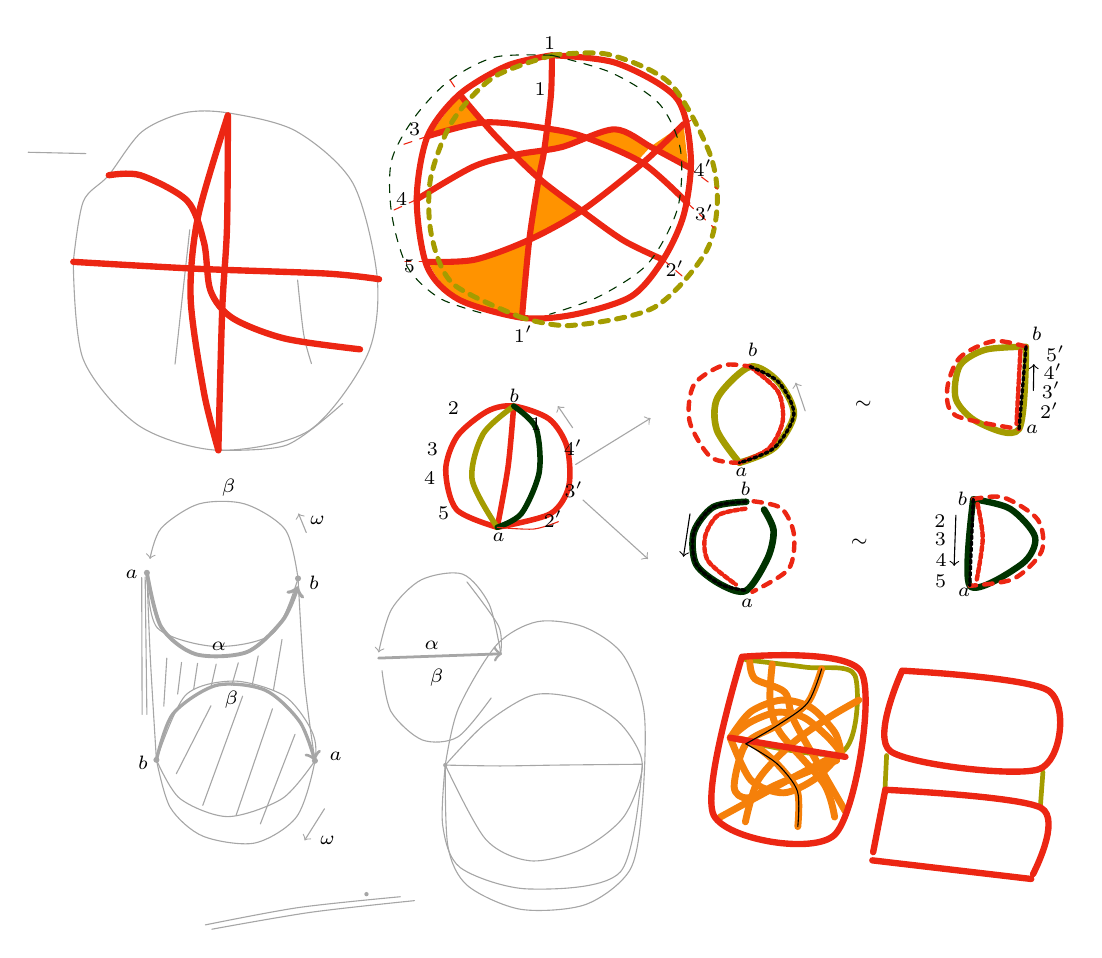
\begin{tikzpicture}[x=.55cm,y=-.55cm,line cap=round,line join=round,g/.style={olive!80!yellow,line width=1.7pt},r/.style={orange!80!brown,line width=1.8pt},w/.style={red!60!black,line width=1.5pt},b/.style={blue!60!black,line width=1.4pt},p/.style={gray!70,thin},k/.style={black,line width=1.2pt},every node/.style={font=\scriptsize}]
\draw[p] plot[smooth] coordinates {(2.85,6.16) (3.08,4.77) (3.66,4.17) (4.43,3.16) (5.41,2.72) (6.42,2.72) (7.99,3.14) (9.31,4.35) (9.87,6.55) (9.64,8.31) (8.29,10.06) (6.2,10.51) (4.36,9.94) (3.08,8.41) (2.85,6.16)};
\draw[p] plot[smooth] coordinates {(1.81,3.63) (3.14,3.66)};
\draw[p] plot[smooth] coordinates {(5.54,5.42) (5.36,7.05) (5.2,8.52)};
\draw[p] plot[smooth] coordinates {(8.03,6.58) (8.17,7.83) (8.35,8.51)};
\draw[p] plot[smooth] coordinates {(6.2,10.51) (7.78,10.39) (9.07,9.43)};
\draw[red!70!brown,line width=2.3pt] plot[smooth] coordinates {(2.85,6.16) (5.71,6.32) (8.69,6.43) (9.91,6.56)};
\draw[red!70!brown,line width=2.3pt] plot[smooth] coordinates {(3.67,4.16) (4.4,4.16) (5.48,4.75) (5.87,5.72) (6.02,6.83) (6.53,7.46) (7.73,7.93) (9.47,8.18)};
\draw[red!70!brown,line width=2.3pt] plot[smooth] coordinates {(6.42,2.78) (5.73,5.12) (5.56,7.0) (5.87,9.19) (6.2,10.51)};
\draw[red!70!brown,line width=2.3pt] plot[smooth] coordinates {(6.42,2.78) (6.4,5.36) (6.29,7.25) (6.2,10.51)};
\fill[orange!85!yellow] (11.1,3.2)--(11.77,2.29)--(12.37,2.95)--cycle;
\fill[orange!85!yellow] (13.78,3.08)--(14.64,3.29)--(13.72,3.58)--cycle;
\fill[orange!85!yellow] (13.08,3.65)--(13.7,3.61)--(13.62,4.17)--cycle;
\fill[orange!85!yellow] (14.66,3.28).. controls (15.2,2.96) and (15.6,3.1)..(16.18,3.5)--(15.86,3.85)--cycle;
\fill[orange!85!yellow] (16.18,3.5)--(16.94,2.98)--(17.05,3.97)--cycle;
\fill[orange!85!yellow] (13.6,4.23)--(14.58,4.97)--(13.38,5.65)--cycle;
\fill[orange!85!yellow] (11.05,6.16).. controls(11.8,6.23) and (12.8,5.94)..(13.38,5.65)--(13.21,7.45).. controls(12.1,7.3) and (11.36,6.91)..(11.05,6.16);
\draw[red!70!brown,line width=2.2pt] plot[smooth] coordinates {(13.9,1.39) (15.39,1.57) (16.78,2.38) (17.11,3.73) (16.95,5.06) (16.47,6.11) (15.73,6.96) (14.4,7.38) (13.21,7.45) (11.75,7.03) (11.02,6.27) (10.78,4.72) (11.03,3.26) (11.77,2.29) (12.87,1.63) (13.9,1.39)};
\draw[red!70!brown,line width=2.2pt] plot[smooth] coordinates {(13.9,1.39) (13.88,2.31) (13.72,3.61) (13.6,4.23) (13.38,5.65) (13.21,7.45)};
\draw[red!70!brown,line width=2.2pt] plot[smooth] coordinates {(11.03,3.26) (12.35,2.94) (13.78,3.08) (14.66,3.28) (16.0,3.88) (17.03,4.8)};
\draw[red!70!brown,line width=2.2pt] plot[smooth] coordinates {(10.78,4.72) (12.09,3.96) (13.1,3.68) (14.13,3.51) (15.35,3.1) (16.21,3.52) (17.05,3.97)};
\draw[red!70!brown,line width=2.2pt] plot[smooth] coordinates {(11.03,6.16) (12.12,6.11) (13.38,5.65) (14.59,4.98) (16.02,3.86) (16.94,2.98)};
\draw[red!70!brown,line width=2.2pt] plot[smooth] coordinates {(11.77,2.29) (12.57,3.22) (13.6,4.23) (14.59,4.98) (15.56,5.67) (16.47,6.11)};
\draw[g,dashed,line width=1.8pt] plot[smooth] coordinates {(13.9,1.39) (15.2,1.37) (16.63,2.04) (17.54,3.64) (17.72,4.81) (17.44,5.96) (16.25,7.22) (14.33,7.63) (13.21,7.45)};
\draw[g,dashed,line width=1.8pt] plot[smooth] coordinates {(13.9,1.39) (12.55,1.9) (11.6,2.92) (11.1,4.24) (11.12,5.54) (11.62,6.67) (13.21,7.45)};
\draw[green!20!black,dashed] plot[smooth] coordinates {(13.9,1.39) (12.6,1.43) (11.55,1.96) (10.74,2.81) (10.2,3.82) (10.2,5.04) (10.56,6.27) (11.31,7.0) (12.38,7.37)};
\draw[green!20!black,dashed] plot[smooth] coordinates {(13.9,1.39) (15.27,1.79) (16.38,2.51) (16.87,3.57) (16.8,4.94) (16.12,6.2) (14.99,6.96) (13.85,7.37)};
\draw[red!70!brown,dashed] plot[smooth] coordinates {(11.55,1.96) (11.77,2.29)};
\draw[red!70!brown,dashed] plot[smooth] coordinates {(11.03,3.26) (10.41,3.47)};
\draw[red!70!brown,dashed] plot[smooth] coordinates {(10.78,4.72) (10.22,4.98)};
\draw[red!70!brown,dashed] plot[smooth] coordinates {(11.03,6.16) (10.51,6.16)};
\draw[red!70!brown,dashed] plot[smooth] coordinates {(16.94,2.98) (17.24,2.83)};
\draw[red!70!brown,dashed] plot[smooth] coordinates {(17.05,3.97) (17.73,4.48)};
\draw[red!70!brown,dashed] plot[smooth] coordinates {(17.03,4.8) (17.65,5.38)};
\draw[red!70!brown,dashed] plot[smooth] coordinates {(16.47,6.11) (16.96,6.53)};
\node at (13.85,1.11) {$\unsure{1}$};
\node at (13.63,2.17) {$1$};
\node at (10.73,3.11) {$3$};
\node at (10.43,4.71) {$4$};
\node at (10.61,6.27) {$5$};
\node at (17.39,4.0) {$4'$};
\node at (17.42,5.03) {$3'$};
\node at (16.74,6.32) {$2'$};
\node at (13.24,7.83) {$\unsure{1'}$};
\draw[red!70!brown,line width=2pt] plot[smooth] coordinates {(12.64,12.29) (11.7,11.88) (11.45,10.96) (11.72,10.18) (12.41,9.61) (13.02,9.49) (13.84,9.79) (14.25,10.43) (14.29,11.35) (13.86,11.98) (12.64,12.29)};
\draw[red!70!brown,line width=2pt] plot[smooth] coordinates {(13.02,9.49) (12.89,10.89) (12.64,12.29)};
\draw[g,line width=2pt] plot[smooth] coordinates {(13.02,9.49) (12.31,10.14) (12.06,11.19) (12.64,12.29)};
\draw[green!20!black,line width=2pt] plot[smooth] coordinates {(13.02,9.49) (13.53,9.99) (13.61,11.01) (13.2,11.97) (12.64,12.29)};
\draw[red!70!brown] plot[smooth] coordinates {(12.64,12.29) (13.48,12.33) (14.05,12.16)};
\draw[p,->] plot[smooth] coordinates {(14.45,10.84) (16.18,9.77)};
\draw[p,->] plot[smooth] coordinates {(14.62,11.66) (16.12,13.02)};
\draw[p,->] plot[smooth] coordinates {(14.38,9.99) (14.04,9.49)};
\node at (12.67,12.53) {$a$};
\node at (13.03,9.25) {$b$};
\node at (11.63,9.53) {$\unsure{2}$};
\node at (11.14,10.48) {$3$};
\node at (11.08,11.15) {$4$};
\node at (11.4,11.96) {$5$};
\node at (14.39,10.45) {$4'$};
\node at (14.41,11.42) {$3'$};
\node at (13.93,12.1) {$2'$};
\node at (13.54,9.9) {$\unsure{1}$};
\draw[g,line width=2.4pt] plot[smooth] coordinates {(18.23,10.8) (17.71,10.04) (17.73,9.29) (18.48,8.58) (19.13,8.93) (19.49,9.68) (19.03,10.46) (18.23,10.8)};
\draw[red!70!brown,dashed,line width=1.6pt] plot[smooth] coordinates {(18.23,10.8) (17.57,10.67) (17.08,9.84) (17.18,9.0) (17.85,8.55) (18.48,8.58)};
\draw[red!70!brown,densely dotted,line width=1.6pt] plot[smooth] coordinates {(18.48,8.58) (19.12,9.15) (19.23,9.84) (18.91,10.47) (18.23,10.8)};
\draw[k,densely dotted] plot[smooth] coordinates {(18.48,8.58) (19.13,8.93) (19.49,9.68) (19.03,10.46) (18.23,10.8)};
\draw[p,->] plot[smooth] coordinates {(19.75,9.6) (19.53,8.95)};
\node at (18.54,8.18) {$b$};
\node at (18.28,11.01) {$a$};
\node at (21.09,9.46) {$\sim$};
\draw[g,line width=2.3pt] plot[smooth] coordinates {(24.85,8.12) (23.91,8.19) (23.32,8.56) (23.23,9.33) (23.75,9.87) (24.69,10.02) (24.85,8.12)};
\draw[red!70!brown,dashed,line width=1.6pt] plot[smooth] coordinates {(24.85,8.12) (24.1,7.99) (23.32,8.37) (23.03,9.1) (23.23,9.71) (24.69,10.02)};
\draw[red!70!brown,densely dotted,line width=1.6pt] plot[smooth] coordinates {(24.72,8.21) (24.63,9.9)};
\draw[k,densely dotted] plot[smooth] coordinates {(24.85,8.12) (24.69,10.02)};
\draw[k,thin,->] plot[smooth] coordinates {(25.02,9.13) (25.03,8.52)};
\node at (25.1,7.83) {$b$};
\node at (24.99,10.02) {$a$};
\node at (25.53,8.28) {$5'$};
\node at (25.47,8.7) {$4'$};
\node at (25.43,9.12) {$3'$};
\node at (25.39,9.59) {$2'$};
\draw[green!20!black,line width=2.4pt] plot[smooth] coordinates {(18.39,11.7) (17.63,11.82) (17.18,12.4) (17.23,13.14) (17.8,13.61) (18.39,13.75) (18.89,12.99) (19.02,12.36) (18.8,11.88)};
\draw[red!70!brown,dashed,line width=1.6pt] plot[smooth] coordinates {(18.56,11.69) (19.2,11.85) (19.49,12.45) (19.37,13.25) (18.53,13.78)};
\draw[red!70!brown,densely dotted,line width=1.6pt] plot[smooth] coordinates {(18.37,11.86) (17.74,12.01) (17.44,12.5) (17.51,13.07) (18.15,13.61)};
\draw[k,densely dotted] plot[smooth] coordinates {(18.39,11.7) (17.63,11.82) (17.18,12.4) (17.23,13.14) (17.8,13.61) (18.39,13.75)};
\draw[k,thin,->] plot[smooth] coordinates {(17.09,11.98) (16.94,12.97)};
\node at (18.37,11.39) {$b$};
\node at (18.41,14.04) {$a$};
\node at (21.0,12.64) {$\sim$};
\draw[green!20!black,line width=2.3pt] plot[smooth] coordinates {(23.63,11.64) (24.48,11.86) (25.06,12.52) (24.75,13.14) (23.55,13.64) (23.63,11.64)};
\draw[red!70!brown,dashed,line width=1.6pt] plot[smooth] coordinates {(23.63,11.64) (24.33,11.6) (25.12,12.11) (25.21,12.84) (24.56,13.48) (23.55,13.64)};
\draw[red!70!brown,densely dotted,line width=1.6pt] plot[smooth] coordinates {(23.73,11.75) (23.85,12.55) (23.71,13.51)};
\draw[k,densely dotted] plot[smooth] coordinates {(23.63,11.64) (23.55,13.64)};
\draw[k,thin,->] plot[smooth] coordinates {(23.23,12.01) (23.19,13.18)};
\node at (23.38,11.62) {$b$};
\node at (23.42,13.8) {$a$};
\node at (22.86,12.14) {$2$};
\node at (22.87,12.57) {$3$};
\node at (22.89,13.06) {$4$};
\node at (22.88,13.54) {$5$};
\draw[p,->] plot[smooth] coordinates {(8.04,13.47) (7.75,12.35) (6.81,11.75) (5.75,11.75) (4.88,12.31) (4.62,13.02)};
\draw[p,line width=1.4pt,->] plot[smooth] coordinates {(4.55,13.34) (4.88,14.59) (5.68,15.22) (6.86,15.17) (7.69,14.43) (8.04,13.65)};
\draw[p] plot[smooth] coordinates {(4.55,13.34) (4.63,15.32) (4.77,17.66)};
\draw[p] plot[smooth] coordinates {(8.04,13.47) (8.19,15.85) (8.43,17.68)};
\draw[p] plot[smooth] coordinates {(4.55,13.34) (4.79,14.61) (6.12,15.04) (7.46,14.74) (8.04,13.47)};
\draw[p,line width=1.2pt,->] plot[smooth] coordinates {(4.77,17.66) (5.15,16.6) (6.15,15.94) (7.28,16.05) (8.08,16.78) (8.43,17.68)};
\draw[p] plot[smooth] coordinates {(4.77,17.66) (5.09,18.76) (5.84,19.42) (7.04,19.58) (8.01,18.97) (8.43,17.68) (8.35,16.98) (7.72,16.18) (6.56,15.84) (5.44,16.17) (4.77,17.66)};
\draw[p] plot[smooth] coordinates {(4.77,17.66) (5.31,18.55) (6.42,18.97) (7.68,18.55) (8.43,17.68)};
\draw[p,->] plot[smooth] coordinates {(8.23,12.41) (8.05,11.97)};
\draw[p,->] plot[smooth] coordinates {(8.65,18.79) (8.19,19.52)};
\draw[p] plot[smooth] coordinates {(4.43,13.45) (4.44,16.61)};
\draw[p] plot[smooth] coordinates {(4.51,13.44) (4.55,16.61)};
\draw[p] plot[smooth] coordinates {(5.01,15.31) (4.94,16.42)};
\draw[p] plot[smooth] coordinates {(5.35,15.41) (5.26,16.14)};
\draw[p] plot[smooth] coordinates {(5.72,15.43) (5.63,16.03)};
\draw[p] plot[smooth] coordinates {(6.15,15.45) (6.03,15.98)};
\draw[p] plot[smooth] coordinates {(6.66,15.42) (6.51,15.94)};
\draw[p] plot[smooth] coordinates {(7.12,15.26) (6.98,15.94)};
\draw[p] plot[smooth] coordinates {(7.67,14.88) (7.47,16.06)};
\draw[p] plot[smooth] coordinates {(5.23,17.98) (6.03,16.41)};
\draw[p] plot[smooth] coordinates {(5.84,18.71) (6.76,16.19)};
\draw[p] plot[smooth] coordinates {(6.61,18.94) (7.45,16.48)};
\draw[p] plot[smooth] coordinates {(7.17,19.14) (7.97,17.07)};
\fill[p] (4.55,13.34) circle (.07);
\fill[p] (8.04,13.47) circle (.07);
\fill[p] (4.77,17.66) circle (.07);
\fill[p] (8.43,17.68) circle (.07);
\node at (4.2,13.37) {$a$};
\node at (8.41,13.57) {$b$};
\node at (4.46,17.73) {$b$};
\node at (8.91,17.58) {$a$};
\node at (6.44,11.38) {$\beta$};
\node at (6.21,15.04) {$\alpha$};
\node at (6.5,16.26) {$\beta$};
\node at (8.49,12.12) {$\omega$};
\node at (8.72,19.51) {$\omega$};
\draw[p,->] plot[smooth] coordinates {(12.72,15.19) (12.45,14.06) (11.84,13.37) (10.89,13.5) (10.2,14.18) (9.9,15.18)};
\draw[p,line width=1pt,->] plot[smooth] coordinates {(9.9,15.31) (12.75,15.21)};
\node at (11.13,15.02) {$\alpha$};
\node at (11.24,15.75) {$\beta$};
\draw[p] plot[smooth] coordinates {(9.98,15.6) (10.19,16.55) (10.91,17.2) (11.73,17.13) (12.5,16.23)};
\draw[p] plot[smooth] coordinates {(12.72,15.19) (12.67,14.57) (11.94,13.55)};
\draw[p] plot[smooth] coordinates {(11.44,17.78) (11.74,16.48) (12.62,15.01) (13.56,14.47) (14.64,14.59) (15.54,15.23) (16.03,16.55) (15.99,18.67) (15.71,20.19) (14.68,21.0) (13.18,21.11) (11.95,20.56) (11.5,19.65) (11.44,17.78)};
\draw[p] plot[smooth] coordinates {(11.44,17.78) (12.7,17.8) (14.03,17.78) (15.99,17.76)};
\draw[p] plot[smooth] coordinates {(11.44,17.78) (12.37,16.82) (13.48,16.16) (14.58,16.27) (15.49,16.83) (15.99,17.76) (15.57,18.96) (14.6,19.72) (13.4,19.99) (12.37,19.49) (11.44,17.78)};
\draw[p] plot[smooth] coordinates {(11.44,17.78) (11.38,19.17) (11.79,20.15) (13.35,20.64) (15.48,20.25) (15.99,17.76)};
\draw[p] plot[smooth] coordinates {(5.9,21.47) (8.05,21.07) (10.4,20.82)};
\draw[p] plot[smooth] coordinates {(6.05,21.57) (8.33,21.18) (10.73,20.91)};
\fill[p] (11.44,17.78) circle (.05);
\fill[p] (9.62,20.76) circle (.05);
\draw[g] plot[smooth] coordinates {(18.38,15.35) (19.76,15.52) (20.9,15.71) (20.58,17.49) (18.02,17.15)};
\draw[g] plot[smooth] coordinates {(21.63,17.56) (21.59,18.4)};
\draw[g] plot[smooth] coordinates {(25.24,17.94) (25.18,18.75)};
\draw[orange!85!brown,line width=2.5pt] plot[smooth] coordinates {(18.47,15.38) (18.59,15.79) (19.28,16.1) (19.52,16.81) (20.68,18.85)};
\draw[orange!85!brown,line width=2.5pt] plot[smooth] coordinates {(18.99,15.45) (18.94,16.31) (19.17,17.03) (20.18,18.21) (20.43,18.98)};
\draw[orange!85!brown,line width=2.5pt] plot[smooth] coordinates {(20.13,15.56) (19.81,16.34) (19.13,16.85) (18.38,17.29) (18.11,18.28) (18.42,18.54) (19.16,18.2) (20.48,17.67)};
\draw[orange!85!brown,line width=2.5pt] plot[smooth] coordinates {(18.02,17.15) (18.49,16.55) (19.2,16.28) (19.88,16.45) (20.43,17.02) (20.58,17.49)};
\draw[orange!85!brown,line width=2.5pt] plot[smooth] coordinates {(18.02,17.15) (18.48,16.79) (19.11,16.56) (19.72,16.68) (20.26,17.12) (20.58,17.49)};
\draw[orange!85!brown,line width=2.5pt] plot[smooth] coordinates {(18.02,17.15) (18.5,18.13) (19.26,18.42) (20.02,18.07) (20.58,17.49)};
\draw[orange!85!brown,line width=2.5pt] plot[smooth] coordinates {(18.02,17.15) (18.49,17.26) (19.09,17.74) (19.57,18.38) (19.58,19.2)};
\draw[orange!85!brown,line width=2.5pt] plot[smooth] coordinates {(20.99,16.28) (20.3,16.68) (19.44,17.29) (18.67,18.12) (18.37,19.09)};
\draw[orange!85!brown,line width=2.5pt] plot[smooth] coordinates {(20.58,17.49) (19.5,18.05) (18.54,18.57) (17.79,18.98)};
\draw[red!70!brown,line width=2.3pt] plot[smooth] coordinates {(18.29,15.28) (21.05,15.64) (20.43,19.39) (17.64,18.94) (18.29,15.28)};
\draw[red!70!brown,line width=2.3pt] plot[smooth] coordinates {(18.02,17.15) (20.68,17.59)};
\draw[red!70!brown,line width=2.3pt] plot[smooth] coordinates {(21.99,15.6) (25.38,16.07) (25.16,17.87) (21.72,17.46) (21.99,15.6)};
\draw[red!70!brown,line width=2.3pt] plot[smooth] coordinates {(21.6,18.35) (25.2,18.77) (25.01,20.3)};
\draw[red!70!brown,line width=2.3pt] plot[smooth] coordinates {(21.6,18.35) (21.32,19.79)};
\draw[red!70!brown,line width=2.3pt] plot[smooth] coordinates {(21.3,19.98) (24.97,20.41)};
\draw[k,thin] plot[smooth] coordinates {(20.13,15.56) (19.81,16.34) (19.13,16.85) (18.38,17.29)};
\draw[k,thin] plot[smooth] coordinates {(18.38,17.29) (19.09,17.74) (19.57,18.38) (19.58,19.2)};
\end{tikzpicture}}
\margin{\mspage{161}}

\scanpage{163}
\figure{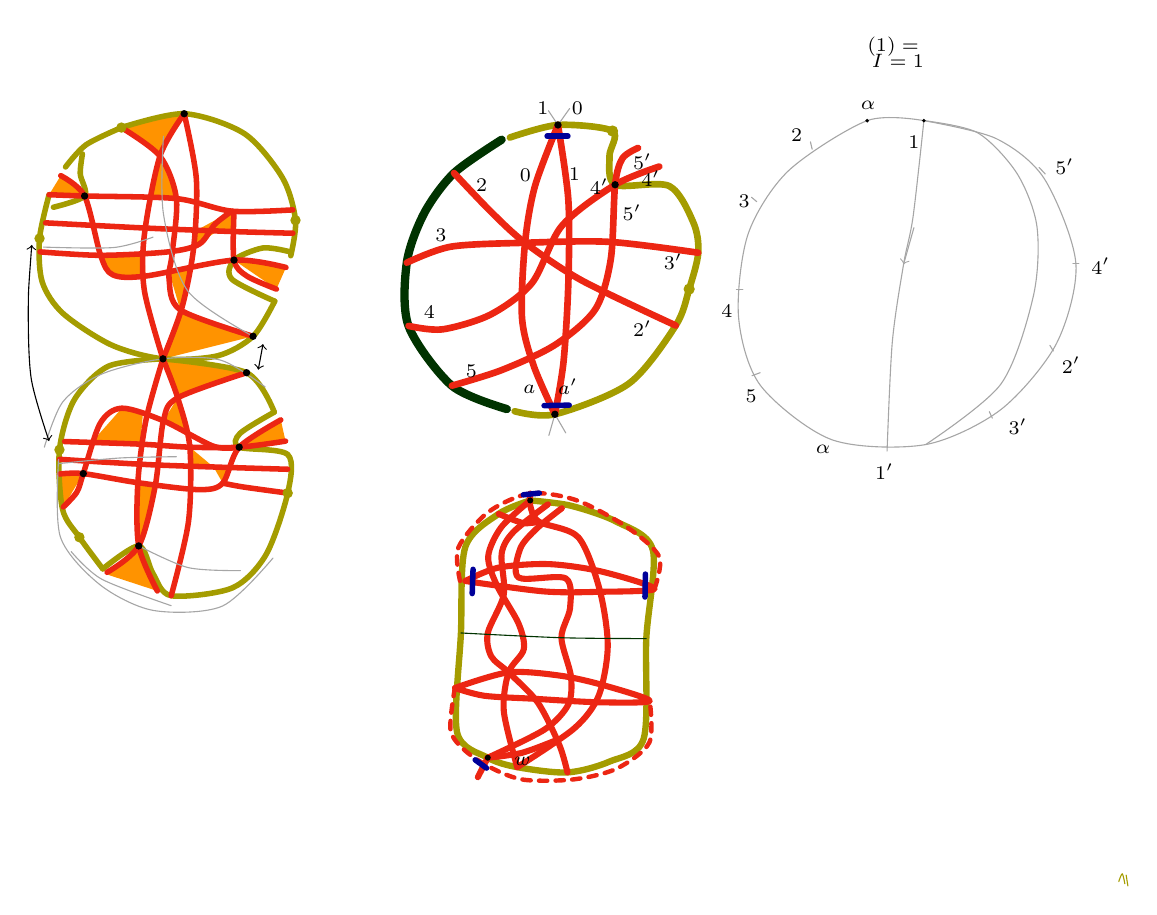
\begin{tikzpicture}[x=.55cm,y=-.55cm,line cap=round,line join=round,g/.style={olive!80!yellow,line width=1.7pt},r/.style={orange!80!brown,line width=1.8pt},w/.style={red!60!black,line width=1.5pt},b/.style={blue!60!black,line width=1.4pt},p/.style={gray!70,thin},k/.style={black,line width=1.2pt},every node/.style={font=\scriptsize}]
\fill[orange!85!yellow] (5.9,3.44)--(7.35,3.12)--(6.79,4.1)--cycle;
\fill[orange!85!yellow] (4.23,4.99)--(4.5,4.55)--(5.05,5.02)--cycle;
\fill[orange!85!yellow] (6.79,4.1)--(7.17,5.08)--(6.55,5.07)--cycle;
\fill[orange!85!yellow] (7.64,5.81)--(8.45,5.37)--(8.45,5.84)--cycle;
\fill[orange!85!yellow] (7.64,5.81)--(7.57,6.2)--(8.04,5.88)--cycle;
\fill[orange!85!yellow] (5.42,6.39)--(6.44,6.39)--(6.45,6.87)--(5.7,6.84)--cycle;
\fill[orange!85!yellow] (7.0,6.77)--(7.45,6.65)--(7.26,7.65)--cycle;
\fill[orange!85!yellow] (7.26,7.65)--(8.94,8.26)--(6.86,8.78)--cycle;
\fill[orange!85!yellow] (8.5,6.5)--(9.7,6.67)--(9.48,7.17)--cycle;
\fill[orange!85!yellow] (6.86,8.78)--(8.79,9.1)--(7.2,9.68)--cycle;
\fill[orange!85!yellow] (5.91,9.92)--(6.4,10.0)--(6.34,10.75)--(5.22,10.7)--cycle;
\fill[orange!85!yellow] (7.2,9.68)--(7.41,10.5)--(6.87,10.21)--cycle;
\fill[orange!85!yellow] (7.48,10.82)--(8.03,11.28)--(7.51,11.31)--cycle;
\fill[orange!85!yellow] (8.03,11.28)--(8.45,11.34)--(8.24,11.65)--cycle;
\fill[orange!85!yellow] (8.62,10.82)--(9.58,10.19)--(9.69,10.68)--cycle;
\fill[orange!85!yellow] (4.47,11.44)--(5.02,11.43)--(4.56,12.2)--cycle;
\fill[orange!85!yellow] (6.28,11.64)--(6.68,11.72)--(6.3,13.1)--cycle;
\fill[orange!85!yellow] (6.3,13.1)--(6.73,14.14)--(5.6,13.77)--cycle;
\draw[g,line width=2pt] plot[smooth] coordinates {(5.9,3.44) (7.35,3.12) (8.74,3.58) (9.62,4.6) (9.92,5.58) (9.81,6.4)};
\draw[g,line width=2pt] plot[smooth] coordinates {(4.61,4.35) (5.08,3.84) (5.9,3.44)};
\draw[g,line width=2pt] plot[smooth] coordinates {(4.23,4.99) (4.01,6.0) (4.07,7.0) (4.55,7.73) (5.67,8.46) (6.86,8.78) (8.12,8.71) (8.94,8.26) (9.44,7.45)};
\draw[g,line width=2pt] plot[smooth] coordinates {(5.0,4.05) (4.95,4.51) (5.05,5.02) (4.33,5.28)};
\draw[g,line width=2pt] plot[smooth] coordinates {(9.8,6.31) (9.17,6.22) (8.5,6.5) (8.45,6.94) (9.44,7.45)};
\draw[g,line width=2pt] plot[smooth] coordinates {(6.86,8.78) (5.6,8.95) (4.81,9.73) (4.47,10.88) (4.54,12.25) (4.93,12.9) (5.47,13.63)};
\draw[g,line width=2pt] plot[smooth] coordinates {(5.47,13.63) (6.3,13.1) (6.63,13.74) (7.05,14.25) (8.46,14.07) (9.24,13.3) (9.74,11.88) (9.74,10.99) (8.62,10.82) (8.64,10.5) (9.43,10.01)};
\draw[g,line width=2pt] plot[smooth] coordinates {(6.86,8.78) (8.79,9.1) (9.43,10.01)};
\draw[red!70!brown,line width=2pt] plot[smooth] coordinates {(5.9,3.44) (6.79,4.1) (7.17,5.08) (7.07,6.36) (7.0,6.94) (7.26,7.65) (8.94,8.26)};
\draw[red!70!brown,line width=2pt] plot[smooth] coordinates {(7.35,3.12) (6.79,4.1) (6.43,5.92) (6.43,7.2) (6.86,8.78)};
\draw[red!70!brown,line width=2pt] plot[smooth] coordinates {(7.35,3.12) (7.63,4.62) (7.57,6.2) (7.3,7.59) (6.86,8.78)};
\draw[red!70!brown,line width=2pt] plot[smooth] coordinates {(4.23,4.99) (5.05,5.02) (7.17,5.08) (8.45,5.37) (9.86,5.34)};
\draw[red!70!brown,line width=2pt] plot[smooth] coordinates {(4.15,5.64) (6.45,5.76) (8.45,5.84) (9.86,5.88)};
\draw[red!70!brown,line width=2pt] plot[smooth] coordinates {(4.02,6.31) (5.42,6.39) (6.98,6.31) (7.7,6.13) (8.06,5.67) (8.45,5.37)};
\draw[red!70!brown,line width=2pt] plot[smooth] coordinates {(4.5,4.55) (5.05,5.02) (5.42,6.39) (5.7,6.84) (6.45,6.87) (8.5,6.5) (9.7,6.67)};
\draw[red!70!brown,line width=2pt] plot[smooth] coordinates {(8.5,5.4) (8.5,6.5) (8.8,6.87) (9.48,7.17)};
\draw[red!70!brown,line width=2pt] plot[smooth] coordinates {(6.86,8.78) (6.47,10.18) (6.28,11.64) (6.3,13.1) (6.73,14.14)};
\draw[red!70!brown,line width=2pt] plot[smooth] coordinates {(6.86,8.78) (7.2,9.68) (7.48,10.82) (7.45,12.53) (7.05,14.25)};
\draw[red!70!brown,line width=2pt] plot[smooth] coordinates {(8.79,9.1) (7.2,9.68) (6.87,10.21) (6.68,11.72) (6.3,13.1) (5.57,13.71)};
\draw[red!70!brown,line width=2pt] plot[smooth] coordinates {(4.59,10.69) (6.34,10.75) (7.48,10.82) (8.62,10.82) (9.69,10.68)};
\draw[red!70!brown,line width=2pt] plot[smooth] coordinates {(4.47,11.1) (6.68,11.23) (9.74,11.33)};
\draw[red!70!brown,line width=2pt] plot[smooth] coordinates {(4.47,11.44) (5.02,11.43) (6.28,11.64) (7.69,11.8) (8.24,11.65) (8.62,10.82) (9.58,10.19)};
\draw[red!70!brown,line width=2pt] plot[smooth] coordinates {(4.56,12.2) (4.87,11.86) (5.02,11.43) (5.41,10.27) (5.91,9.92) (6.87,10.21) (8.03,10.8) (8.62,10.82)};
\draw[red!70!brown,line width=2pt] plot[smooth] coordinates {(8.24,11.65) (8.72,11.74) (9.74,11.88)};
\draw[p] plot[smooth] coordinates {(4.1,6.2) (5.72,6.21) (6.63,5.97)};
\draw[p] plot[smooth] coordinates {(6.87,3.64) (6.87,5.43) (7.43,7.21) (8.94,8.26)};
\draw[p] plot[smooth] coordinates {(4.12,10.82) (4.55,9.77) (5.45,9.13) (6.86,8.78) (8.19,8.81) (9.22,9.43)};
\draw[p] plot[smooth] coordinates {(4.45,11.1) (4.49,12.89) (5.41,14.0) (6.64,14.59) (8.23,14.49) (9.4,13.38)};
\draw[p] plot[smooth] coordinates {(4.45,11.2) (5.86,11.07) (7.17,11.04)};
\draw[p] plot[smooth] coordinates {(6.3,13.1) (7.44,13.6) (8.65,13.67)};
\draw[p] plot[smooth] coordinates {(4.74,13.23) (5.45,13.87) (7.05,14.48)};
\draw[k,thin,<->] plot[smooth] coordinates {(3.83,6.15) (3.75,7.64) (3.82,9.25) (4.23,10.68)};
\draw[k,thin,<->] plot[smooth] coordinates {(9.17,8.44) (9.06,9.03)};
\fill[k] (7.35,3.12) circle (.085);
\fill[k] (5.05,5.02) circle (.085);
\fill[k] (8.5,6.5) circle (.085);
\fill[k] (8.94,8.26) circle (.085);
\fill[k] (6.86,8.78) circle (.085);
\fill[k] (8.79,9.1) circle (.085);
\fill[k] (5.02,11.43) circle (.085);
\fill[k] (8.62,10.82) circle (.085);
\fill[k] (6.3,13.1) circle (.085);
\fill[g] (5.9,3.44) circle (.12);
\fill[g] (4.01,6.0) circle (.12);
\fill[g] (9.92,5.58) circle (.12);
\fill[g] (4.47,10.88) circle (.12);
\fill[g] (9.74,11.88) circle (.12);
\fill[g] (4.93,12.9) circle (.12);
\draw[green!20!black,line width=3pt] plot[smooth] coordinates {(14.68,3.72) (13.58,4.49) (12.89,5.42) (12.49,6.56) (12.53,8.02) (13.53,9.4) (14.8,9.94)};
\draw[g,line width=2.4pt] plot[smooth] coordinates {(14.87,3.67) (15.98,3.38) (17.24,3.52) (17.17,4.1) (17.3,4.76) (18.55,4.79) (19.11,5.64) (19.22,6.33) (19.01,7.17) (18.7,8.01) (17.62,9.35) (15.91,10.06) (14.98,9.99)};
\draw[red!70!brown,line width=2.4pt] plot[smooth] coordinates {(15.98,3.38) (15.45,4.79) (15.22,6.1) (15.15,7.83) (15.42,8.94) (15.91,10.06)};
\draw[red!70!brown,line width=2.4pt] plot[smooth] coordinates {(15.98,3.38) (16.22,5.11) (16.22,7.03) (16.11,8.84) (15.91,10.06)};
\draw[red!70!brown,line width=2.4pt] plot[smooth] coordinates {(13.58,4.49) (14.44,5.39) (15.22,6.1) (16.53,6.97) (18.7,8.01)};
\draw[red!70!brown,line width=2.4pt] plot[smooth] coordinates {(12.49,6.56) (13.51,6.19) (15.22,6.1) (17.18,6.08) (19.22,6.33)};
\draw[red!70!brown,line width=2.4pt] plot[smooth] coordinates {(12.53,8.02) (13.31,8.1) (14.42,7.76) (15.38,7.03) (16.07,5.71) (17.3,4.76) (18.32,4.34)};
\draw[red!70!brown,line width=2.4pt] plot[smooth] coordinates {(13.53,9.4) (14.68,9.04) (15.91,8.46) (16.84,7.64) (17.2,6.48) (17.3,4.76) (17.47,4.15) (17.83,3.91)};
\draw[blue!60!black,line width=2pt] plot[smooth] coordinates {(15.73,3.64) (16.21,3.64)};
\draw[blue!60!black,line width=2pt] plot[smooth] coordinates {(15.66,9.86) (16.24,9.85)};
\draw[p] plot[smooth] coordinates {(15.98,3.38) (16.25,3.0)};
\draw[p] plot[smooth] coordinates {(15.98,3.38) (15.76,3.05)};
\draw[p] plot[smooth] coordinates {(15.91,10.06) (15.77,10.55)};
\draw[p] plot[smooth] coordinates {(15.91,10.06) (16.16,10.49)};
\fill[k] (15.98,3.38) circle (.085);
\fill[k] (15.91,10.06) circle (.085);
\fill[k] (17.3,4.76) circle (.085);
\fill[g] (17.24,3.52) circle (.13);
\fill[g] (19.01,7.17) circle (.13);
\node at (15.63,3.0) {$1$};
\node at (16.43,2.99) {$0$};
\node at (15.23,4.55) {$\unsure{0}$};
\node at (16.36,4.51) {$1$};
\node at (14.22,4.77) {$2$};
\node at (13.28,5.93) {$3$};
\node at (13.01,7.71) {$4$};
\node at (13.98,9.07) {$5$};
\node at (18.64,6.54) {$3'$};
\node at (17.93,8.08) {$2'$};
\node at (17.69,5.4) {$5'$};
\node at (17.93,4.23) {$5'$};
\node at (18.12,4.62) {$4'$};
\node at (16.93,4.81) {$4'$};
\node at (15.32,9.49) {$a$};
\node at (16.21,9.42) {$a'$};
\draw[p] plot[smooth] coordinates {(24.43,3.28) (26.09,3.69) (27.21,4.62) (27.94,6.58) (27.49,8.43) (26.21,9.95) (24.47,10.76) (22.31,10.65) (20.66,9.4) (20.15,7.81) (20.37,5.9) (21.3,4.44) (23.12,3.28) (24.43,3.28)};
\draw[p] plot[smooth] coordinates {(24.43,3.28) (25.67,3.56) (26.58,4.5) (27.04,5.72) (26.96,7.32) (26.21,9.36) (24.47,10.76)};
\draw[p] plot[smooth] coordinates {(24.43,3.28) (24.18,5.5) (23.96,6.6) (23.7,8.4) (23.58,10.91)};
\draw[p,->] plot[smooth] coordinates {(24.2,5.75) (23.96,6.6)};
\draw[p] plot[smooth] coordinates {(21.81,3.77) (21.85,3.94)};
\draw[p] plot[smooth] coordinates {(20.45,5.05) (20.57,5.15)};
\draw[p] plot[smooth] coordinates {(20.1,7.17) (20.25,7.17)};
\draw[p] plot[smooth] coordinates {(20.46,9.17) (20.65,9.1)};
\draw[p] plot[smooth] coordinates {(27.09,4.36) (27.23,4.51)};
\draw[p] plot[smooth] coordinates {(27.87,6.58) (28.01,6.58)};
\draw[p] plot[smooth] coordinates {(27.34,8.47) (27.42,8.6)};
\draw[p] plot[smooth] coordinates {(25.94,10.0) (26.01,10.15)};
\fill[k] (23.12,3.28) circle (.045);
\fill[k] (24.43,3.28) circle (.045);
\node at (23.14,2.93) {$\alpha$};
\node at (24.2,3.78) {$1$};
\node at (21.49,3.62) {$2$};
\node at (20.28,5.13) {$3$};
\node at (19.88,7.68) {$4$};
\node at (20.44,9.64) {$5$};
\node at (27.68,4.35) {$5'$};
\node at (28.51,6.64) {$4'$};
\node at (27.83,8.93) {$\unsure{2'}$};
\node at (26.6,10.35) {$\unsure{3'}$};
\node at (23.52,11.38) {$1'$};
\node at (22.1,10.87) {$\unsure{\alpha}$};
\draw[g,line width=2.3pt] plot[smooth] coordinates {(15.34,12.05) (14.61,12.36) (13.84,13.13) (13.74,15.11) (13.65,17.4) (14.36,17.99) (15.05,18.21) (16.2,18.33) (17.17,18.08) (17.96,17.55) (18.02,15.24) (18.17,13.19) (17.33,12.54) (16.27,12.17) (15.34,12.05)};
\draw[red!70!brown,dashed,line width=1.6pt] plot[smooth] coordinates {(13.72,13.91) (13.68,13.14) (14.37,12.32) (15.34,11.89) (16.42,12.05) (17.58,12.67) (18.32,13.35) (18.21,14.09)};
\draw[red!70!brown,dashed,line width=1.6pt] plot[smooth] coordinates {(13.6,16.38) (13.5,17.35) (13.84,17.83) (14.47,18.24) (15.2,18.5) (16.35,18.49) (17.34,18.24) (18.09,17.64) (18.1,16.68)};
\draw[red!70!brown,line width=2.2pt] plot[smooth] coordinates {(13.84,13.91) (14.61,13.6) (15.77,13.52) (16.98,13.69) (18.21,14.09) (16.92,14.16) (15.65,14.15) (13.84,13.91)};
\draw[red!70!brown,line width=2.2pt] plot[smooth] coordinates {(13.6,16.38) (14.84,16.02) (16.06,16.1) (17.08,16.33) (18.1,16.68) (16.91,16.71) (15.44,16.63) (14.28,16.56) (13.6,16.38)};
\draw[red!70!brown,line width=2.2pt] plot[smooth] coordinates {(15.34,11.89) (15.34,12.17) (15.54,12.54) (16.45,12.9) (16.94,14.1) (17.13,15.41) (16.92,16.56) (16.36,17.31) (15.04,18.21)};
\draw[red!70!brown,line width=2.2pt] plot[smooth] coordinates {(15.34,12.05) (14.67,12.67) (14.37,13.34) (14.57,14.01) (15.07,14.89) (15.19,15.49) (14.84,16.02) (14.73,16.92) (15.04,18.21)};
\draw[red!70!brown,line width=2.2pt] plot[smooth] coordinates {(15.75,12.14) (14.95,12.78) (14.68,13.28) (14.73,14.22) (14.36,15.11) (14.44,15.65) (14.84,16.02) (15.51,16.71) (16.01,17.69) (16.2,18.33)};
\draw[red!70!brown,line width=2.2pt] plot[smooth] coordinates {(16.07,12.23) (15.5,12.69) (15.11,13.16) (15.07,13.83) (16.16,13.85) (16.26,14.53) (16.06,15.22) (16.28,16.11) (16.22,16.76) (15.67,17.34) (14.36,17.99)};
\draw[red!70!brown,line width=2.2pt] plot[smooth] coordinates {(14.36,17.99) (15.14,17.88) (15.93,17.59)};
\draw[red!70!brown,line width=2.2pt] plot[smooth] coordinates {(14.36,17.99) (14.13,18.44)};
\draw[red!70!brown,line width=2.2pt] plot[smooth] coordinates {(14.61,12.36) (15.17,12.57) (15.54,12.54)};
\draw[green!20!black] plot[smooth] coordinates {(13.74,15.11) (16.06,15.22) (18.02,15.24)};
\draw[blue!60!black,line width=2pt] plot[smooth] coordinates {(15.18,11.92) (15.55,11.88)};
\draw[blue!60!black,line width=2pt] plot[smooth] coordinates {(14.02,13.64) (14.0,14.2)};
\draw[blue!60!black,line width=2pt] plot[smooth] coordinates {(18.0,13.75) (17.99,14.28)};
\draw[blue!60!black,line width=2pt] plot[smooth] coordinates {(14.07,18.04) (14.33,18.23)};
\fill[k] (15.34,12.05) circle (.07);
\fill[k] (14.36,17.99) circle (.07);
\node at (15.16,18.08) {$\unsure{w}$};
\node at (23.72,1.57) {$\unsure{(1)}=$};
\node at (23.83,1.91) {$\unsure{I=1}$};
\draw[g,thin] plot[smooth] coordinates {(28.93,20.85) (29.01,20.67) (29.07,20.9)};
\draw[g,thin] plot[smooth] coordinates {(29.1,20.7) (29.14,20.95)};
\end{tikzpicture}}
\margin{\mspage{162}}

\scanpage{164}
{\scriptsize\ttfamily\begin{tabular}{lllll}
1 & //CRAY2 JOB '\unsure{********}, & ',' & ', & JOB 0411\\
 & // MSGLEVEL=(1,1) & & &\\
2 & // EXEC PGM=IEFBR14 & & &
\end{tabular}}
\figure{\begin{tikzpicture}[x=.55cm,y=-.55cm,line cap=round,line join=round,g/.style={olive!80!yellow,line width=1.7pt},r/.style={orange!80!brown,line width=1.8pt},w/.style={red!60!black,line width=1.5pt},b/.style={blue!60!black,line width=1.4pt},p/.style={gray!70,thin},k/.style={black,line width=1.2pt},every node/.style={font=\scriptsize}]
\draw[g,line width=1.6pt] plot[smooth] coordinates {(4.71,10.73) (6.2,8.72) (7.83,7.24) (9.09,6.5) (11.06,5.65) (12.4,5.3) (14.49,5.28) (16.12,5.78) (17.33,6.84) (17.87,8.28) (17.87,9.75) (17.29,11.32) (16.23,12.23) (14.84,12.72) (13.48,12.59) (12.19,11.88) (10.85,10.64) (9.99,9.21) (9.46,7.7) (9.09,6.5) (8.85,4.69) (8.79,2.42)};
\draw[g,line width=1.6pt] plot[smooth] coordinates {(5.29,13.35) (6.72,11.52) (8.21,10.15) (9.99,9.21) (11.09,8.9) (12.4,8.85) (14.68,9.27) (17.87,9.75) (19.8,9.71) (20.93,9.06) (21.2,8.02) (20.9,6.25) (20.42,4.86) (19.7,3.62) (18.31,1.48)};
\draw[yellow!70!brown,line width=1.5pt] plot[smooth] coordinates {(7.14,15.58) (8.91,13.24) (10.85,10.64) (12.4,8.85) (14.41,7.12) (16.12,5.78) (17.79,4.72) (19.7,3.62) (21.81,2.75)};
\draw[g,thin] plot[smooth] coordinates {(7.99,14.26) (8.39,14.12) (9.09,13.08)};
\draw[g,thin] plot[smooth] coordinates {(4.71,10.73) (6.2,8.72) (7.83,7.24) (9.09,6.5)};
\draw[b,line width=2.8pt] plot[smooth] coordinates {(4.63,10.52) (4.86,10.12)};
\draw[b,line width=2.8pt] plot[smooth] coordinates {(5.44,13.33) (5.8,12.94)};
\draw[b,line width=2.8pt] plot[smooth] coordinates {(7.09,15.3) (7.57,14.69)};
\draw[b,line width=2.8pt] plot[smooth] coordinates {(8.72,2.48) (8.73,3.08)};
\draw[b,line width=2.8pt] plot[smooth] coordinates {(18.45,1.52) (18.69,1.84)};
\draw[b,line width=2.8pt] plot[smooth] coordinates {(21.2,2.84) (21.75,2.65)};
\draw[b,line width=2.8pt] plot[smooth] coordinates {(8.95,6.31) (8.91,6.47) (9.07,6.51)};
\draw[b,line width=2.8pt] plot[smooth] coordinates {(15.99,5.63) (16.2,5.64) (16.3,5.73)};
\draw[b,line width=2.8pt] plot[smooth] coordinates {(12.22,8.88) (12.29,9.04)};
\draw[b,line width=2.8pt] plot[smooth] coordinates {(17.99,9.79) (17.84,9.94)};
\draw[b,line width=2.8pt] plot[smooth] coordinates {(10.76,10.42) (10.74,10.59)};
\draw[b,line width=2.8pt] plot[smooth] coordinates {(10.0,9.13) (10.1,9.26)};
\draw[k,->] plot[smooth] coordinates {(9.12,6.49) (9.01,5.96)};
\draw[k,->] plot[smooth] coordinates {(9.12,6.49) (8.58,6.79)};
\draw[k,->] plot[smooth] coordinates {(16.1,5.76) (15.61,5.57)};
\draw[k,->] plot[smooth] coordinates {(16.14,5.77) (16.62,5.53)};
\draw[k,->] plot[smooth] coordinates {(19.7,3.62) (19.55,3.22)};
\draw[k,->] plot[smooth] coordinates {(19.7,3.62) (20.12,3.48)};
\draw[k,->] plot[smooth] coordinates {(17.87,9.75) (18.41,9.75)};
\draw[k,->] plot[smooth] coordinates {(17.87,9.75) (17.68,10.28)};
\draw[k,->] plot[smooth] coordinates {(12.4,8.85) (11.95,8.85)};
\draw[k,->] plot[smooth] coordinates {(12.4,8.85) (12.15,9.25)};
\draw[k,->] plot[smooth] coordinates {(9.99,9.21) (9.63,9.33)};
\draw[k,->] plot[smooth] coordinates {(9.99,9.21) (10.2,9.52)};
\draw[k,->] plot[smooth] coordinates {(10.85,10.64) (10.66,10.14)};
\draw[k,->] plot[smooth] coordinates {(10.85,10.64) (10.56,10.96)};
\node at (12.41,5.17) {$+$};
\node at (17.87,4.76) {$+$};
\node at (20.93,8.49) {$+$};
\node at (15.43,12.43) {$+$};
\node at (11.47,9.99) {$+$};
\node at (10.98,8.91) {$+$};
\node at (9.48,7.82) {$-$};
\node at (14.04,7.4) {$-$};
\node at (18.0,7.79) {$-$};
\node at (14.94,9.32) {$-$};
\node at (10.42,9.84) {$-$};
\end{tikzpicture}}
\margin{\mspage{163}}

\scanpage{165}
{\ttfamily //* GUTS 0108 I}
\figure{\begin{tikzpicture}[x=.55cm,y=-.55cm,line cap=round,line join=round,g/.style={olive!80!yellow,line width=1.7pt},r/.style={orange!80!brown,line width=1.8pt},w/.style={red!60!black,line width=1.5pt},b/.style={blue!60!black,line width=1.4pt},p/.style={gray!70,thin},k/.style={black,line width=1.2pt},every node/.style={font=\scriptsize}]
\draw[g,line width=2pt] plot[smooth] coordinates {(3.74,7.02) (4.37,6.51) (5.6,5.35) (6.67,4.31) (7.24,3.84)};
\draw[g,line width=2pt] plot[smooth] coordinates {(4.03,3.85) (4.6,4.41) (5.6,5.35) (6.58,6.45) (7.18,6.99)};
\draw[orange!85!brown,line width=2pt] plot[smooth] coordinates {(4.29,3.39) (3.91,4.25) (3.88,4.83)};
\draw[orange!85!brown,line width=2pt] plot[smooth] coordinates {(3.65,4.75) (4.3,4.57) (4.6,4.41) (5.05,3.93)};
\draw[orange!85!brown,line width=2pt] plot[smooth] coordinates {(6.9,3.35) (7.27,3.86) (7.45,4.58) (7.43,4.94)};
\draw[orange!85!brown,line width=2pt] plot[smooth] coordinates {(6.23,4.16) (6.67,4.48) (7.16,4.61) (7.79,4.49)};
\draw[orange!85!brown,line width=2pt] plot[smooth] coordinates {(3.94,5.93) (4.37,6.51) (4.66,7.03) (4.71,7.49)};
\draw[orange!85!brown,line width=2pt] plot[smooth] coordinates {(3.32,6.69) (3.74,7.02) (4.22,7.24) (5.0,7.29)};
\draw[orange!85!brown,line width=2pt] plot[smooth] coordinates {(6.97,6.02) (6.58,6.45) (6.34,6.94) (6.32,7.41)};
\draw[orange!85!brown,line width=2pt] plot[smooth] coordinates {(6.11,7.17) (6.84,7.13) (7.43,6.94) (7.66,6.6)};
\draw[orange!85!brown,line width=2pt] plot[smooth] coordinates {(5.62,4.89) (5.61,5.83)};
\draw[orange!85!brown,line width=2pt] plot[smooth] coordinates {(5.27,5.22) (5.96,5.36)};
\draw[blue!40!black,line width=4pt] plot[smooth] coordinates {(4.03,3.85) (4.6,4.41)};
\draw[blue!40!black,line width=4pt] plot[smooth] coordinates {(6.67,4.31) (7.24,3.84)};
\draw[blue!40!black,line width=4pt] plot[smooth] coordinates {(3.74,7.02) (4.37,6.51)};
\draw[blue!40!black,line width=4pt] plot[smooth] coordinates {(6.58,6.45) (7.18,6.99)};
\draw[orange!85!brown,line width=1.8pt] plot[smooth] coordinates {(4.71,4.66) (5.2,4.51)};
\draw[orange!85!brown,line width=1.8pt] plot[smooth] coordinates {(4.81,4.9) (5.35,4.72)};
\draw[orange!85!brown,line width=1.8pt] plot[smooth] coordinates {(4.94,5.02) (5.41,4.87)};
\draw[orange!85!brown,line width=1.8pt] plot[smooth] coordinates {(5.97,4.76) (6.3,5.21)};
\draw[orange!85!brown,line width=1.8pt] plot[smooth] coordinates {(6.19,4.59) (6.56,4.97)};
\draw[orange!85!brown,line width=1.8pt] plot[smooth] coordinates {(6.25,4.83) (6.47,4.87)};
\draw[orange!85!brown,line width=1.8pt] plot[smooth] coordinates {(4.63,5.66) (5.11,5.84)};
\draw[orange!85!brown,line width=1.8pt] plot[smooth] coordinates {(4.93,5.45) (5.37,5.67)};
\draw[orange!85!brown,line width=1.8pt] plot[smooth] coordinates {(5.17,5.84) (5.31,5.48)};
\draw[orange!85!brown,line width=1.8pt] plot[smooth] coordinates {(5.85,5.98) (6.05,5.59)};
\draw[orange!85!brown,line width=1.8pt] plot[smooth] coordinates {(6.11,6.18) (6.3,5.84)};
\draw[orange!85!brown,line width=1.8pt] plot[smooth] coordinates {(5.88,5.64) (6.32,5.51)};
\draw[k,dashed,thin] plot[smooth] coordinates {(3.59,4.24) (3.7,4.57) (4.2,4.7) (4.65,4.62) (5.6,5.35) (4.97,6.15) (4.74,7.22) (4.31,7.57)};
\draw[k,dashed,thin] plot[smooth] coordinates {(7.58,4.37) (7.35,4.7) (6.8,4.84) (6.32,4.73) (5.6,5.35) (6.23,6.05) (6.38,6.7) (6.28,7.18) (6.79,7.62)};
\draw[g] plot[smooth] coordinates {(9.07,.87) (9.78,1.97) (11.13,3.43) (12.54,5.05)};
\draw[g] plot[smooth] coordinates {(9.32,5.21) (11.13,3.43) (13.17,1.52)};
\draw[k,thin] plot[smooth] coordinates {(9.28,1.23) (11.13,3.43) (12.75,5.54)};
\draw[k,thin] plot[smooth] coordinates {(9.32,5.21) (11.13,3.43) (13.17,1.52)};
\draw[orange!85!brown,line width=2.2pt] plot[smooth] coordinates {(11.1,1.62) (11.13,3.43) (11.18,4.52)};
\draw[orange!85!brown,line width=2.2pt] plot[smooth] coordinates {(9.84,3.44) (11.13,3.43) (12.58,3.44)};
\draw[orange!85!brown,line width=2.2pt] plot[smooth] coordinates {(9.99,1.26) (9.78,1.97) (9.54,2.66)};
\draw[orange!85!brown,line width=2.2pt] plot[smooth] coordinates {(8.99,2.31) (9.78,1.97) (10.68,1.64)};
\draw[orange!85!brown,line width=2.2pt] plot[smooth] coordinates {(12.78,1.33) (12.81,2.58)};
\draw[orange!85!brown,line width=2.2pt] plot[smooth] coordinates {(12.35,1.79) (13.46,2.29)};
\draw[orange!85!brown,line width=2.2pt] plot[smooth] coordinates {(9.78,3.9) (9.79,5.53)};
\draw[orange!85!brown,line width=2.2pt] plot[smooth] coordinates {(9.42,4.61) (10.43,5.12)};
\draw[orange!85!brown,line width=2.2pt] plot[smooth] coordinates {(12.73,4.48) (12.18,5.63)};
\draw[orange!85!brown,line width=2.2pt] plot[smooth] coordinates {(11.84,5.03) (13.12,5.04)};
\draw[orange!85!brown,line width=1.7pt] plot[smooth] coordinates {(10.14,2.65) (10.45,2.43)};
\draw[orange!85!brown,line width=1.7pt] plot[smooth] coordinates {(10.41,2.99) (10.8,2.66)};
\draw[orange!85!brown,line width=1.7pt] plot[smooth] coordinates {(11.65,2.48) (11.69,3.0)};
\draw[orange!85!brown,line width=1.7pt] plot[smooth] coordinates {(11.91,2.35) (12.03,2.8)};
\draw[orange!85!brown,line width=1.7pt] plot[smooth] coordinates {(12.15,2.27) (12.3,2.59)};
\draw[orange!85!brown,line width=1.7pt] plot[smooth] coordinates {(11.67,3.88) (11.94,3.79)};
\draw[orange!85!brown,line width=1.7pt] plot[smooth] coordinates {(11.83,4.14) (12.19,3.95)};
\draw[orange!85!brown,line width=1.7pt] plot[smooth] coordinates {(12.0,4.36) (12.45,4.09)};
\draw[orange!85!brown,line width=1.7pt] plot[smooth] coordinates {(10.11,4.03) (10.52,4.22)};
\draw[orange!85!brown,line width=1.7pt] plot[smooth] coordinates {(10.26,3.88) (10.62,4.02)};
\draw[orange!85!brown,line width=1.7pt] plot[smooth] coordinates {(10.49,3.82) (10.74,3.95)};
\draw[green!20!black,line width=1.8pt] plot[smooth] coordinates {(9.09,.75) (9.03,1.07)};
\draw[green!20!black,line width=1.8pt] plot[smooth] coordinates {(9.25,.91) (9.19,1.25)};
\draw[green!20!black,line width=1.8pt] plot[smooth] coordinates {(9.4,1.07) (9.31,1.44)};
\draw[green!20!black,line width=1.8pt] plot[smooth] coordinates {(11.36,3.1) (11.34,3.32)};
\draw[green!20!black,line width=1.8pt] plot[smooth] coordinates {(11.46,2.99) (11.47,3.22)};
\draw[green!20!black,line width=1.8pt] plot[smooth] coordinates {(11.59,2.85) (11.59,3.11)};
\draw[green!20!black,line width=1.8pt] plot[smooth] coordinates {(11.72,2.72) (11.72,3.0)};
\draw[green!20!black,dashed,line width=1.6pt] plot[smooth] coordinates {(9.31,1.27) (9.77,1.37) (10.18,1.88) (10.18,2.39)};
\draw[green!20!black,dashed,line width=1.6pt] plot[smooth] coordinates {(12.23,2.57) (12.41,1.93) (12.85,1.58) (13.19,1.47)};
\draw[green!20!black,dashed,line width=1.6pt] plot[smooth] coordinates {(10.12,4.32) (9.6,4.45) (9.33,5.08)};
\draw[green!20!black,dashed,line width=1.6pt] plot[smooth] coordinates {(12.09,4.46) (12.66,4.67) (12.82,5.15) (12.78,5.51)};
\fill[green!20!black] (9.78,1.97)--(9.42,2.13)--(9.59,2.35)--cycle;
\fill[green!20!black] (12.81,2.01)--(12.84,2.42)--(13.11,2.22)--cycle;
\fill[green!20!black] (9.79,4.88)--(9.89,5.31)--(10.15,5.1)--cycle;
\fill[green!20!black] (12.54,5.05)--(12.1,5.1)--(12.29,5.4)--cycle;
\draw[green!20!black] plot[smooth] coordinates {(10.97,3.85) (11.2,3.89) (11.43,3.8)};
\draw[g,line width=2pt] plot[smooth] coordinates {(20.11,5.98) (22.22,4.38) (24.94,1.8) (26.1,.9)};
\draw[g,line width=2pt] plot[smooth] coordinates {(20.39,2.25) (22.22,4.38) (24.01,6.47)};
\draw[g,line width=2pt] plot[smooth] coordinates {(23.62,.56) (24.94,1.8) (26.1,3.12)};
\draw[g,line width=2pt] plot[smooth] coordinates {(8.1,11.14) (8.59,12.04) (9.12,12.96)};
\draw[g,line width=2pt] plot[smooth] coordinates {(7.84,12.39) (9.34,11.66)};
\draw[g,thin] plot[smooth] coordinates {(23.65,4.16) (23.63,4.63)};
\end{tikzpicture}}
{\scriptsize\ttfamily\begin{tabular}{llll}
\ GGGGGGGGGG\  & UU\ \ \ \ \ \ \ \ UU & TTTTTTTTTTTT & \ SSSSSSSSSS\ \\
GGGGGGGGGGGG & UU\ \ \ \ \ \ \ \ UU & TTTTTTTTTTTT & SSSSSSSSSSSS\\
GG\ \ \ \ \ \ \ \ GG & UU\ \ \ \ \ \ \ \ UU & \ \ \ \ \ TT\ \ \ \ \  & SS\ \ \ \ \ \ \ \ SS\\
GG\ \ \ \ \ \ \ \ \ \  & UU\ \ \ \ \ \ \ \ UU & \ \ \ \ \ TT\ \ \ \ \  & SS\ \ \ \ \ \ \ \ \ \ \\
GG\ \ \ \ \ \ \ \ \ \  & UU\ \ \ \ \ \ \ \ UU & \ \ \ \ \ TT\ \ \ \ \  & SSS\ \ \ \ \ \ \ \ \ \\
GG\ \ \ \ \ \ \ \ \ \  & UU\ \ \ \ \ \ \ \ UU & \ \ \ \ \ TT\ \ \ \ \  & \ SSSSSSSSS\ \ \\
GG\ \ \ \ \ GGGGG & UU\ \ \ \ \ \ \ \ UU & \ \ \ \ \ TT\ \ \ \ \  & \ \ SSSSSSSSS\ \\
GG\ \ \ \ \ GGGGG & UU\ \ \ \ \ \ \ \ UU & \ \ \ \ \ TT\ \ \ \ \  & \ \ \ \ \ \ \ \ \ SSS\\
GG\ \ \ \ \ \ \ \ GG & UU\ \ \ \ \ \ \ \ UU & \ \ \ \ \ TT\ \ \ \ \  & \ \ \ \ \ \ \ \ \ \ SS\\
GG\ \ \ \ \ \ \ \ GG & UU\ \ \ \ \ \ \ \ UU & \ \ \ \ \ TT\ \ \ \ \  & SS\ \ \ \ \ \ \ \ SS\\
GGGGGGGGGGGG & UUUUUUUUUUUU & \ \ \ \ \ TT\ \ \ \ \  & SSSSSSSSSSSS\\
\ GGGGGGGGGG\  & \ UUUUUUUUUU\  & \ \ \ \ \ TT\ \ \ \ \  & \ SSSSSSSSSS\ \\
\end{tabular}}
{\scriptsize\ttfamily\begin{tabular}{l}
****P END STC 108 GUTS ROOM 4.07.01 PM 16 AUG 82 R6.PR1 SYS JES2 STC 108 END P****\\
****P END STC 108 GUTS ROOM 4.07.01 PM 16 AUG 82 R6.PR1 SYS JES2 STC 108 END P****\\
****P END STC 108 GUTS ROOM 4.07.01 PM 16 AUG 82 R6.PR1 SYS JES2 STC 108 END P****\\
****P END STC 108 GUTS ROOM 4.07.01 PM 16 AUG 82 R6.PR1 SYS JES2 STC 108 END P****\\
****P END STC 108 GUTS ROOM 4.07.01 PM 16 AUG 82 R6.PR1 SYS JES2 STC 108 END P****\\
****P END STC 108 GUTS ROOM 4.07.01 PM 16 AUG 82 R6.PR1 SYS JES2 STC 108 END P****\\
\end{tabular}}
\figure{\begin{tikzpicture}[x=.55cm,y=-.55cm,line cap=round,line join=round,g/.style={olive!80!yellow,line width=1.7pt},r/.style={orange!80!brown,line width=1.8pt},w/.style={red!60!black,line width=1.5pt},b/.style={blue!60!black,line width=1.4pt},p/.style={gray!70,thin},k/.style={black,line width=1.2pt},every node/.style={font=\scriptsize}]
\draw[g,line width=2pt] plot[smooth] coordinates {(3.9,14.53) (2.93,14.72) (2.3,15.63) (2.31,16.62) (2.92,17.23) (3.51,17.37) (3.33,17.76) (2.67,18.18) (2.38,19.01) (2.67,19.72) (3.33,20.03)};
\draw[g,line width=2pt] plot[smooth] coordinates {(3.94,14.53) (4.79,14.91) (5.11,15.83) (4.89,16.87) (4.22,17.38) (4.29,17.72) (4.86,18.08) (5.08,18.81) (4.88,19.6) (4.21,20.05)};
\draw[g,line width=2pt] plot[smooth] coordinates {(3.53,20.02) (3.66,19.94) (4.08,19.96)};
\draw[g,line width=2pt] plot[smooth] coordinates {(7.0,14.86) (6.73,14.64) (6.15,14.89) (5.78,15.7) (5.88,16.68) (6.57,17.32) (6.7,17.64) (7.09,17.76) (7.47,17.51) (7.6,17.22) (8.24,16.75) (8.51,15.81) (8.17,14.94) (7.49,14.67) (7.34,14.87)};
\draw[orange!85!brown,line width=2.6pt] plot[smooth] coordinates {(3.84,14.52) (3.66,16.15) (3.63,17.37) (4.05,18.62) (3.91,20.0) (3.87,20.32)};
\draw[orange!85!brown,line width=2.6pt] plot[smooth] coordinates {(3.97,14.55) (4.1,15.89) (4.02,17.36) (3.6,18.57) (3.66,19.94)};
\draw[orange!85!brown,line width=2.6pt] plot[smooth] coordinates {(7.11,14.48) (6.99,15.75) (6.93,17.33) (7.14,17.59)};
\draw[orange!85!brown,line width=2.6pt] plot[smooth] coordinates {(7.3,14.49) (7.4,15.68) (7.2,17.42) (7.04,17.61)};
\draw[orange!85!brown,line width=2.6pt] plot[smooth] coordinates {(7.11,14.48) (7.38,14.23)};
\draw[orange!85!brown,line width=2.6pt] plot[smooth] coordinates {(7.3,14.49) (7.16,14.25)};
\draw[k,dashed] plot[smooth] coordinates {(3.9,14.43) (2.83,14.58) (2.23,15.49) (2.16,16.34) (2.58,17.12) (3.41,17.48) (3.23,17.72) (2.58,17.98) (2.27,18.82) (2.39,19.58) (2.91,20.13) (3.43,20.19) (3.6,20.01)};
\draw[k,dashed] plot[smooth] coordinates {(3.9,14.43) (4.82,14.74) (5.25,15.56) (5.2,16.55) (4.78,17.19) (4.3,17.5) (4.82,17.74) (5.23,18.38) (5.24,19.29) (4.79,19.92) (4.2,20.18)};
\draw[k,dashed] plot[smooth] coordinates {(7.02,14.56) (6.55,14.46) (5.99,14.7) (5.7,15.46) (5.68,16.23) (5.99,16.99) (6.51,17.5) (6.65,17.84) (7.13,17.94) (7.7,17.61) (8.16,17.09) (8.62,16.18) (8.58,15.45) (8.16,14.65) (7.56,14.49) (7.35,14.75) (7.02,14.56)};
\draw[p] plot[smooth] coordinates {(3.87,14.66) (2.88,14.98) (2.45,15.68) (2.44,16.44) (3.2,17.2)};
\draw[p] plot[smooth] coordinates {(3.99,14.69) (4.67,15.02) (4.88,15.82) (4.67,16.87)};
\draw[p] plot[smooth] coordinates {(3.28,17.82) (2.68,18.33) (2.59,19.2) (3.03,19.82)};
\draw[p] plot[smooth] coordinates {(4.26,17.81) (4.74,18.26) (4.79,19.1) (4.31,19.7)};
\draw[p] plot[smooth] coordinates {(6.93,14.89) (6.37,14.96) (6.01,15.69) (6.08,16.48) (6.66,17.19)};
\draw[p] plot[smooth] coordinates {(7.49,14.88) (8.04,15.18) (8.29,15.93) (8.01,16.68) (7.45,17.2)};
\draw[k,line width=2.4pt] plot[smooth] coordinates {(3.48,17.34) (4.2,17.37)};
\draw[k,line width=2.4pt] plot[smooth] coordinates {(3.46,17.49) (4.19,17.5)};
\draw[k,line width=2.4pt] plot[smooth] coordinates {(6.72,17.68) (7.1,17.79) (7.46,17.63)};
\draw[k,thin,->] plot[smooth] coordinates {(5.09,16.22) (5.1,15.79)};
\draw[k,thin,->] plot[smooth] coordinates {(8.49,16.19) (8.49,15.85)};
\draw[k,thin,->] plot[smooth] coordinates {(4.91,18.87) (5.07,18.47)};
\node at (3.54,14.92) {$D$};
\node at (4.29,14.93) {$D'$};
\node at (3.39,16.02) {$\unsure{D}$};
\node at (3.39,17.24) {$D$};
\node at (4.2,17.2) {$D'$};
\node at (3.6,17.76) {$\unsure{x'}$};
\node at (4.02,17.76) {$\unsure{y'}$};
\node at (3.4,19.6) {$D$};
\node at (4.26,19.46) {$D'$};
\node at (6.75,14.99) {$D$};
\node at (7.59,14.98) {$D'$};
\node at (6.67,17.6) {$\unsure{D'}$};
\node at (7.59,17.48) {$\unsure{D}$};
\node at (6.92,17.43) {$\unsure{x'}$};
\node at (7.25,17.43) {$\unsure{y'}$};
\draw[g,line width=2pt] plot[smooth] coordinates {(6.12,18.61) (6.61,19.11) (7.86,19.13) (8.42,18.71)};
\draw[g,line width=2pt] plot[smooth] coordinates {(6.0,20.71) (6.72,20.15) (7.83,20.13) (8.47,20.57)};
\draw[g,line width=2pt] plot[smooth] coordinates {(6.61,19.11) (6.72,20.15)};
\draw[g,line width=2pt] plot[smooth] coordinates {(7.86,19.13) (7.83,20.13)};
\draw[orange!85!brown,line width=3pt] plot[smooth] coordinates {(6.98,19.16) (7.34,19.7) (7.55,20.1)};
\draw[orange!85!brown,line width=3pt] plot[smooth] coordinates {(7.54,19.16) (7.34,19.7) (7.09,20.1)};
\draw[blue!40!black,line width=4pt] plot[smooth] coordinates {(6.61,19.11) (7.86,19.13)};
\draw[k] plot[smooth] coordinates {(6.68,19.2) (6.74,19.66) (7.8,19.67) (7.85,19.21)};
\draw[k] plot[smooth] coordinates {(6.74,20.1) (7.8,20.11)};
\node at (6.61,18.91) {$\unsure{x_0|v_0}$};
\node at (7.05,18.94) {$x$};
\node at (7.48,18.93) {$y$};
\node at (7.93,18.94) {$y_0$};
\node at (6.54,20.12) {$\unsure{x'_0}$};
\node at (7.1,20.42) {$x'$};
\node at (7.48,20.44) {$y'$};
\node at (7.99,20.22) {$y'_0$};
\draw[green!20!black,line width=2pt] plot[smooth] coordinates {(10.24,15.99) (10.53,16.43) (10.27,18.17) (9.81,18.6)};
\draw[green!20!black,line width=2pt] plot[smooth] coordinates {(11.19,18.25) (11.52,18.69)};
\draw[green!20!black,line width=2pt] plot[smooth] coordinates {(12.04,16.64) (12.54,16.65)};
\draw[green!20!black,line width=2pt] plot[smooth] coordinates {(13.34,18.53) (13.62,18.03) (13.66,17.3) (13.78,16.55) (14.02,16.08)};
\draw[green!20!black,line width=2pt] plot[smooth] coordinates {(14.45,17.89) (14.93,18.17)};
\draw[g,line width=2pt] plot[smooth] coordinates {(10.53,16.43) (11.3,16.61) (12.04,16.64) (11.65,17.27) (11.19,18.25) (10.72,18.12) (10.27,18.17) (10.53,16.43)};
\draw[g,line width=2pt] plot[smooth] coordinates {(12.54,16.65) (13.78,16.55) (13.66,17.3) (14.17,17.93) (13.62,18.03) (13.03,17.38) (12.54,16.65)};
\draw[g,line width=2pt] plot[smooth] coordinates {(14.14,15.89) (14.4,15.09) (15.36,14.8) (14.99,15.73) (14.14,15.89)};
\draw[g,line width=2pt] plot[smooth] coordinates {(15.04,18.31) (16.31,18.25) (16.22,19.01) (15.16,18.99) (15.04,18.31)};
\draw[g,line width=2pt] plot[smooth] coordinates {(13.26,18.83) (12.51,19.09) (13.02,20.38) (13.75,20.03) (13.26,18.83)};
\draw[g] plot[smooth] coordinates {(10.58,16.52) (10.39,17.94)};
\draw[g] plot[smooth] coordinates {(10.75,16.57) (10.52,18.1)};
\draw[g] plot[smooth] coordinates {(10.95,16.6) (10.66,18.11)};
\draw[g] plot[smooth] coordinates {(11.16,16.63) (10.83,18.13)};
\draw[g] plot[smooth] coordinates {(11.39,16.66) (11.01,18.18)};
\draw[g] plot[smooth] coordinates {(11.62,16.7) (11.2,18.2)};
\draw[g] plot[smooth] coordinates {(11.81,16.72) (11.42,17.62)};
\draw[g] plot[smooth] coordinates {(12.7,16.73) (13.25,16.65)};
\draw[g] plot[smooth] coordinates {(12.89,16.91) (13.53,16.64)};
\draw[g] plot[smooth] coordinates {(13.02,17.09) (13.61,16.7)};
\draw[g] plot[smooth] coordinates {(13.16,17.28) (13.64,16.88)};
\draw[g] plot[smooth] coordinates {(13.28,17.47) (13.64,17.09)};
\draw[g] plot[smooth] coordinates {(13.43,17.67) (13.72,17.36)};
\draw[g] plot[smooth] coordinates {(13.59,17.85) (13.87,17.62)};
\draw[g] plot[smooth] coordinates {(14.46,15.15) (14.24,15.83)};
\draw[g] plot[smooth] coordinates {(14.68,15.07) (14.46,15.8)};
\draw[g] plot[smooth] coordinates {(14.89,15.01) (14.67,15.76)};
\draw[g] plot[smooth] coordinates {(15.1,14.94) (14.87,15.76)};
\draw[g] plot[smooth] coordinates {(15.26,18.39) (15.21,18.88)};
\draw[g] plot[smooth] coordinates {(15.48,18.37) (15.34,18.89)};
\draw[g] plot[smooth] coordinates {(15.7,18.36) (15.53,18.87)};
\draw[g] plot[smooth] coordinates {(15.93,18.35) (15.76,18.87)};
\draw[g] plot[smooth] coordinates {(16.12,18.33) (15.97,18.88)};
\draw[g] plot[smooth] coordinates {(12.65,19.15) (13.12,20.22)};
\draw[g] plot[smooth] coordinates {(12.91,19.06) (13.26,20.11)};
\draw[g] plot[smooth] coordinates {(13.19,18.97) (13.44,20.04)};
\draw[g] plot[smooth] coordinates {(13.26,19.34) (13.01,20.13)};
\draw[orange!85!brown,line width=2.5pt] plot[smooth] coordinates {(11.89,15.74) (11.9,16.47) (12.28,17.15) (12.65,17.77) (12.67,18.4)};
\draw[orange!85!brown,line width=2.5pt] plot[smooth] coordinates {(12.72,15.7) (12.54,16.65) (12.28,17.15) (12.06,17.65) (12.13,18.45)};
\draw[orange!85!brown,line width=2.5pt] plot[smooth] coordinates {(13.61,15.72) (14.02,16.08) (14.39,16.77)};
\draw[orange!85!brown,line width=2.5pt] plot[smooth] coordinates {(13.3,16.27) (13.78,16.55) (14.59,16.34)};
\draw[orange!85!brown,line width=2.5pt] plot[smooth] coordinates {(13.11,18.16) (13.62,18.03) (14.04,18.5)};
\draw[orange!85!brown,line width=2.5pt] plot[smooth] coordinates {(12.98,18.65) (13.61,18.64) (14.04,18.5)};
\draw[orange!85!brown,line width=2.5pt] plot[smooth] coordinates {(14.39,17.73) (14.35,18.25) (14.55,18.81)};
\draw[orange!85!brown,line width=2.5pt] plot[smooth] coordinates {(15.09,18.05) (14.74,18.49) (14.35,18.6)};
\draw[blue!40!black,line width=3pt] plot[smooth] coordinates {(12.04,16.59) (12.54,16.6)};
\draw[k,dashed,thin] plot[smooth] coordinates {(11.9,16.84) (11.83,17.13) (12.28,17.15) (12.7,17.1) (13.34,16.65) (13.83,16.77)};
\draw[k,dashed,thin] plot[smooth] coordinates {(14.2,15.85) (14.3,16.27) (14.16,16.66)};
\draw[k,dashed,thin] plot[smooth] coordinates {(13.62,18.03) (13.78,18.47) (13.43,18.8) (13.24,18.9)};
\draw[k,dashed,thin] plot[smooth] coordinates {(14.22,17.88) (14.18,18.32) (14.36,18.6) (14.92,18.46)};
\node at (12.75,16.64) {$u_0$};
\node at (12.82,17.22) {$b$};
\node at (13.15,16.81) {$u$};
\node at (13.94,16.91) {$y$};
\node at (14.46,16.11) {$a$};
\node at (13.53,18.02) {$x_0$};
\node at (14.05,17.96) {$u$};
\node at (14.63,17.91) {$u_0$};
\node at (13.72,19.0) {$a$};
\node at (14.85,18.83) {$b$};
\draw[g] plot[smooth] coordinates {(17.51,17.46) (19.06,17.39) (21.0,17.28) (23.73,17.1)};
\draw[g,dashed] plot[smooth] coordinates {(17.59,17.62) (19.75,17.6) (23.41,17.38)};
\draw[orange!85!brown,line width=2.7pt] plot[smooth] coordinates {(18.42,15.83) (18.64,16.6) (19.26,18.13)};
\draw[orange!85!brown,line width=2.7pt] plot[smooth] coordinates {(18.77,15.99) (18.64,16.6) (18.34,18.08)};
\draw[orange!85!brown,line width=2.7pt] plot[smooth] coordinates {(21.98,15.58) (22.17,16.16) (22.78,18.17)};
\draw[orange!85!brown,line width=2.7pt] plot[smooth] coordinates {(22.25,15.58) (22.17,16.16) (21.9,18.0)};
\draw[k] plot[smooth] coordinates {(17.51,17.46) (17.78,17.27) (18.06,16.79) (18.64,16.6) (19.12,16.6) (19.43,17.15) (19.78,17.34)};
\draw[k] plot[smooth] coordinates {(17.86,16.59) (19.31,16.59)};
\draw[k] plot[smooth] coordinates {(21.0,17.28) (21.29,17.06) (21.58,16.29) (22.17,16.16) (22.87,16.2) (23.16,16.8) (23.73,17.1)};
\draw[k] plot[smooth] coordinates {(21.55,16.18) (23.04,16.16)};
\node at (17.74,16.63) {$a$};
\node at (21.37,16.22) {$b$};
\node at (18.32,17.3) {$x_0$};
\node at (19.14,17.31) {$y_0$};
\node at (21.88,17.06) {$u_0$};
\node at (22.77,17.04) {$v_0$};
\node at (17.56,17.61) {$x$};
\node at (19.79,17.52) {$y$};
\node at (21.06,17.44) {$u$};
\node at (23.8,17.21) {$v$};
\end{tikzpicture}}
\margin{\mspage{164}}

\scanpage{166}
\figure{\begin{tikzpicture}[x=.55cm,y=-.55cm,line cap=round,line join=round,g/.style={olive!80!yellow,line width=1.7pt},r/.style={orange!80!brown,line width=1.8pt},w/.style={red!60!black,line width=1.5pt},b/.style={blue!60!black,line width=1.4pt},p/.style={gray!70,thin},k/.style={black,line width=1.2pt},every node/.style={font=\scriptsize}]
\draw[g,line width=1.8pt] plot[smooth] coordinates {(1.57,7.57) (4.19,6.23) (5.47,5.6) (6.64,4.94) (8.03,4.22) (9.52,3.16) (10.6,2.18) (12.29,.2)};
\draw[g,line width=1.8pt] plot[smooth] coordinates {(3.17,10.17) (4.52,8.85) (5.84,7.78) (7.13,6.85) (8.12,6.36) (10.43,5.5) (11.87,4.99) (13.1,4.62) (14.26,4.46) (16.47,4.58) (18.06,4.94) (19.58,5.55) (20.71,6.56) (21.49,7.81) (21.72,9.26) (21.52,10.56) (20.59,11.8) (18.9,12.55) (17.73,12.82) (16.05,12.68) (14.77,12.34) (13.55,11.84) (12.12,10.96) (10.83,10.12) (9.72,9.17) (8.89,8.33) (7.94,7.6) (7.13,6.85) (6.34,6.25) (5.47,5.6) (3.85,4.92) (2.1,4.55)};
\draw[g,line width=1.8pt] plot[smooth] coordinates {(4.8,12.1) (5.96,10.59) (7.56,9.25) (8.89,8.33) (10.43,7.59) (11.56,6.94) (12.57,6.22) (13.57,5.34) (14.26,4.46) (14.81,3.36) (14.99,2.78) (14.92,.95)};
\draw[g,line width=1.8pt] plot[smooth] coordinates {(7.02,14.8) (8.46,12.95) (9.72,11.44) (10.83,10.12) (11.31,9.55) (12.52,8.23) (13.34,7.3) (14.99,6.04) (16.78,4.54) (18.24,3.55) (19.91,2.59) (21.49,1.94)};
\draw[g,line width=1.8pt] plot[smooth] coordinates {(10.11,16.85) (11.45,14.73) (12.47,13.13) (13.55,11.84) (14.6,10.78) (15.45,10.04) (16.69,9.41) (18.08,8.8) (19.6,8.42) (21.49,7.81) (23.14,7.13) (23.67,6.43) (23.61,5.66) (23.29,5.01) (22.06,3.87) (19.91,2.59) (17.53,1.08)};
\draw[yellow!70!brown,line width=1.5pt] plot[smooth] coordinates {(10.09,.64) (10.6,2.18) (11.13,3.51) (11.87,4.99) (12.17,5.51) (12.57,6.22) (13.0,6.86) (13.34,7.3) (13.82,7.95) (14.41,8.8) (15.45,10.04) (16.68,11.52) (17.73,12.82) (19.23,14.57) (20.96,16.06)};
\draw[green!20!black,line width=3pt] plot[smooth] coordinates {(7.3,1.67) (7.51,3.07) (7.85,4.08)};
\draw[green!20!black,line width=3pt] plot[smooth] coordinates {(8.95,5.97) (9.57,6.82) (10.29,7.5)};
\draw[green!20!black,line width=3pt] plot[smooth] coordinates {(11.87,9.04) (13.33,9.81) (14.6,10.78)};
\draw[green!20!black,line width=3pt] plot[smooth] coordinates {(16.05,12.68) (16.78,14.26) (17.76,16.45)};
\draw[black!70!brown,line width=3pt] plot[smooth] coordinates {(8.03,4.22) (8.43,5.1) (8.95,5.97)};
\draw[black!70!brown,line width=3pt] plot[smooth] coordinates {(10.43,7.59) (11.05,8.33) (11.87,9.04)};
\draw[black!70!brown,line width=3pt] plot[smooth] coordinates {(14.6,10.78) (15.31,11.5) (16.05,12.68)};
\draw[orange!75!brown,line width=1.8pt] plot[smooth] coordinates {(6.64,4.94) (7.27,5.39) (8.12,6.36) (8.8,6.81) (9.47,8.04) (10.39,8.46) (11.31,9.55) (12.52,10.16) (14.05,11.26) (14.77,12.34) (15.42,13.11) (15.63,13.66)};
\draw[orange!75!brown,line width=1.8pt] plot[smooth] coordinates {(9.52,3.16) (9.73,4.37) (10.06,5.03) (10.43,5.5) (10.59,6.14) (10.99,6.57) (11.56,6.94) (11.74,7.57) (12.06,7.99) (12.52,8.23) (13.34,9.14) (14.13,9.77) (15.09,10.3) (15.79,11.3) (16.89,12.78) (17.18,13.74)};
\draw[orange!75!brown,line width=1.8pt] plot[smooth] coordinates {(6.64,4.94) (7.13,5.83) (8.12,6.36)};
\draw[orange!75!brown,line width=1.8pt] plot[smooth] coordinates {(9.52,3.16) (10.01,4.03) (10.43,5.5)};
\draw[orange!75!brown,line width=1.8pt] plot[smooth] coordinates {(9.47,8.04) (10.24,8.51) (10.8,9.11) (11.31,9.55)};
\draw[orange!75!brown,line width=1.8pt] plot[smooth] coordinates {(9.47,8.04) (10.1,8.78) (10.71,9.26) (11.31,9.55)};
\draw[orange!75!brown,line width=1.8pt] plot[smooth] coordinates {(11.56,6.94) (12.11,7.32) (12.52,8.23)};
\draw[orange!75!brown,line width=1.8pt] plot[smooth] coordinates {(11.31,9.55) (12.56,10.32) (14.05,11.26)};
\draw[orange!75!brown,line width=1.8pt] plot[smooth] coordinates {(11.31,9.55) (12.16,9.79) (13.08,10.5) (14.05,11.26)};
\draw[orange!75!brown,line width=1.8pt] plot[smooth] coordinates {(12.52,10.16) (12.59,9.59) (12.88,9.23) (13.34,9.14)};
\draw[orange!75!brown,line width=1.8pt] plot[smooth] coordinates {(12.52,10.16) (12.94,9.72) (13.34,9.14)};
\draw[orange!75!brown,line width=1.8pt] plot[smooth] coordinates {(12.52,10.16) (13.13,9.73) (13.34,9.14)};
\draw[orange!75!brown,line width=1.8pt] plot[smooth] coordinates {(14.05,11.26) (14.28,11.79) (14.77,12.34)};
\draw[orange!75!brown,line width=1.8pt] plot[smooth] coordinates {(15.09,10.3) (15.82,10.82) (16.28,11.66) (16.89,12.78)};
\draw[orange!75!brown,line width=1.6pt] plot[smooth] coordinates {(7.27,5.39) (8.52,4.37) (9.58,3.87)};
\draw[orange!75!brown,line width=1.6pt] plot[smooth] coordinates {(7.39,5.64) (8.85,4.95) (9.65,4.31)};
\draw[orange!75!brown,line width=1.6pt] plot[smooth] coordinates {(7.54,5.81) (9.76,4.61)};
\draw[orange!75!brown,line width=1.6pt] plot[smooth] coordinates {(7.74,6.0) (9.84,4.74)};
\draw[orange!75!brown,line width=1.6pt] plot[smooth] coordinates {(8.8,6.81) (10.45,5.86)};
\draw[orange!75!brown,line width=1.6pt] plot[smooth] coordinates {(8.96,7.1) (10.62,6.17)};
\draw[orange!75!brown,line width=1.6pt] plot[smooth] coordinates {(9.12,7.38) (10.77,6.36)};
\draw[orange!75!brown,line width=1.6pt] plot[smooth] coordinates {(9.27,7.55) (10.9,6.52)};
\draw[orange!75!brown,line width=1.6pt] plot[smooth] coordinates {(9.4,7.73) (11.01,6.65)};
\draw[orange!75!brown,line width=1.6pt] plot[smooth] coordinates {(10.39,8.46) (11.74,7.57)};
\draw[orange!75!brown,line width=1.6pt] plot[smooth] coordinates {(10.77,8.87) (12.04,7.99)};
\draw[k,dashed,thin] plot[smooth] coordinates {(11.72,9.95) (12.35,10.4) (13.31,10.9)};
\draw[orange!75!brown,line width=1.5pt] plot[smooth] coordinates {(3.604,4.878) (4.096,4.962)};
\draw[orange!75!brown,line width=1.5pt] plot[smooth] coordinates {(3.763,4.685) (3.937,5.155)};
\draw[orange!75!brown,line width=1.5pt] plot[smooth] coordinates {(4.010,4.728) (3.690,5.112)};
\draw[orange!75!brown,line width=1.5pt] plot[smooth] coordinates {(3.924,6.184) (4.456,6.276)};
\draw[orange!75!brown,line width=1.5pt] plot[smooth] coordinates {(4.097,5.977) (4.283,6.483)};
\draw[orange!75!brown,line width=1.5pt] plot[smooth] coordinates {(4.363,6.022) (4.017,6.438)};
\draw[orange!75!brown,line width=1.5pt] plot[smooth] coordinates {(6.074,6.204) (6.606,6.296)};
\draw[orange!75!brown,line width=1.5pt] plot[smooth] coordinates {(6.247,5.997) (6.433,6.503)};
\draw[orange!75!brown,line width=1.5pt] plot[smooth] coordinates {(6.513,6.042) (6.167,6.458)};
\draw[orange!75!brown,line width=1.5pt] plot[smooth] coordinates {(6.334,4.888) (6.946,4.992)};
\draw[orange!75!brown,line width=1.5pt] plot[smooth] coordinates {(6.533,4.649) (6.747,5.231)};
\draw[orange!75!brown,line width=1.5pt] plot[smooth] coordinates {(6.838,4.702) (6.442,5.178)};
\draw[orange!75!brown,line width=1.5pt] plot[smooth] coordinates {(6.824,6.798) (7.436,6.902)};
\draw[orange!75!brown,line width=1.5pt] plot[smooth] coordinates {(6.951,6.597) (7.309,7.103)};
\draw[orange!75!brown,line width=1.5pt] plot[smooth] coordinates {(7.182,6.544) (7.078,7.156)};
\draw[orange!75!brown,line width=1.5pt] plot[smooth] coordinates {(7.383,6.671) (6.877,7.029)};
\draw[orange!75!brown,line width=1.5pt] plot[smooth] coordinates {(5.564,7.733) (6.116,7.827)};
\draw[orange!75!brown,line width=1.5pt] plot[smooth] coordinates {(5.743,7.517) (5.937,8.043)};
\draw[orange!75!brown,line width=1.5pt] plot[smooth] coordinates {(6.019,7.565) (5.661,7.995)};
\draw[orange!75!brown,line width=1.5pt] plot[smooth] coordinates {(7.684,7.556) (8.196,7.644)};
\draw[orange!75!brown,line width=1.5pt] plot[smooth] coordinates {(7.850,7.356) (8.030,7.844)};
\draw[orange!75!brown,line width=1.5pt] plot[smooth] coordinates {(8.106,7.400) (7.774,7.800)};
\draw[orange!75!brown,line width=1.5pt] plot[smooth] coordinates {(7.264,9.199) (7.856,9.301)};
\draw[orange!75!brown,line width=1.5pt] plot[smooth] coordinates {(7.456,8.969) (7.664,9.531)};
\draw[orange!75!brown,line width=1.5pt] plot[smooth] coordinates {(7.752,9.019) (7.368,9.481)};
\draw[orange!75!brown,line width=1.5pt] plot[smooth] coordinates {(9.205,3.106) (9.835,3.214)};
\draw[orange!75!brown,line width=1.5pt] plot[smooth] coordinates {(9.409,2.860) (9.631,3.460)};
\draw[orange!75!brown,line width=1.5pt] plot[smooth] coordinates {(9.725,2.914) (9.315,3.406)};
\draw[orange!75!brown,line width=1.5pt] plot[smooth] coordinates {(10.243,5.468) (10.617,5.532)};
\draw[orange!75!brown,line width=1.5pt] plot[smooth] coordinates {(10.364,5.322) (10.496,5.678)};
\draw[orange!75!brown,line width=1.5pt] plot[smooth] coordinates {(10.551,5.354) (10.309,5.646)};
\draw[orange!75!brown,line width=1.5pt] plot[smooth] coordinates {(10.686,3.434) (11.574,3.586)};
\draw[orange!75!brown,line width=1.5pt] plot[smooth] coordinates {(10.816,3.188) (11.444,3.832)};
\draw[orange!75!brown,line width=1.5pt] plot[smooth] coordinates {(11.065,3.065) (11.195,3.955)};
\draw[orange!75!brown,line width=1.5pt] plot[smooth] coordinates {(11.339,3.112) (10.921,3.908)};
\draw[orange!75!brown,line width=1.5pt] plot[smooth] coordinates {(11.534,3.311) (10.726,3.709)};
\draw[orange!75!brown,line width=1.5pt] plot[smooth] coordinates {(11.835,5.452) (12.505,5.568)};
\draw[orange!75!brown,line width=1.5pt] plot[smooth] coordinates {(11.974,5.232) (12.366,5.788)};
\draw[orange!75!brown,line width=1.5pt] plot[smooth] coordinates {(12.228,5.175) (12.112,5.845)};
\draw[orange!75!brown,line width=1.5pt] plot[smooth] coordinates {(12.448,5.314) (11.892,5.706)};
\draw[orange!75!brown,line width=1.5pt] plot[smooth] coordinates {(12.704,4.603) (13.256,4.697)};
\draw[orange!75!brown,line width=1.5pt] plot[smooth] coordinates {(12.883,4.387) (13.077,4.913)};
\draw[orange!75!brown,line width=1.5pt] plot[smooth] coordinates {(13.159,4.435) (12.801,4.865)};
\draw[orange!75!brown,line width=1.5pt] plot[smooth] coordinates {(13.314,5.296) (13.826,5.384)};
\draw[orange!75!brown,line width=1.5pt] plot[smooth] coordinates {(13.480,5.096) (13.660,5.584)};
\draw[orange!75!brown,line width=1.5pt] plot[smooth] coordinates {(13.736,5.140) (13.404,5.540)};
\draw[orange!75!brown,line width=1.5pt] plot[smooth] coordinates {(14.596,2.712) (15.384,2.848)};
\draw[orange!75!brown,line width=1.5pt] plot[smooth] coordinates {(14.851,2.405) (15.129,3.155)};
\draw[orange!75!brown,line width=1.5pt] plot[smooth] coordinates {(15.246,2.472) (14.734,3.088)};
\draw[orange!75!brown,line width=1.5pt] plot[smooth] coordinates {(15.213,4.409) (15.687,4.491)};
\draw[orange!75!brown,line width=1.5pt] plot[smooth] coordinates {(15.367,4.225) (15.533,4.675)};
\draw[orange!75!brown,line width=1.5pt] plot[smooth] coordinates {(15.603,4.265) (15.297,4.635)};
\draw[orange!75!brown,line width=1.5pt] plot[smooth] coordinates {(16.494,4.491) (17.066,4.589)};
\draw[orange!75!brown,line width=1.5pt] plot[smooth] coordinates {(16.680,4.268) (16.880,4.812)};
\draw[orange!75!brown,line width=1.5pt] plot[smooth] coordinates {(16.965,4.317) (16.595,4.763)};
\draw[orange!75!brown,line width=1.5pt] plot[smooth] coordinates {(17.875,3.487) (18.605,3.613)};
\draw[orange!75!brown,line width=1.5pt] plot[smooth] coordinates {(18.112,3.203) (18.368,3.897)};
\draw[orange!75!brown,line width=1.5pt] plot[smooth] coordinates {(18.477,3.265) (18.003,3.835)};
\draw[orange!75!brown,line width=1.5pt] plot[smooth] coordinates {(19.225,5.489) (19.935,5.611)};
\draw[orange!75!brown,line width=1.5pt] plot[smooth] coordinates {(19.455,5.212) (19.705,5.888)};
\draw[orange!75!brown,line width=1.5pt] plot[smooth] coordinates {(19.810,5.273) (19.350,5.827)};
\draw[orange!75!brown,line width=1.5pt] plot[smooth] coordinates {(22.906,4.944) (23.674,5.076)};
\draw[orange!75!brown,line width=1.5pt] plot[smooth] coordinates {(23.155,4.644) (23.425,5.376)};
\draw[orange!75!brown,line width=1.5pt] plot[smooth] coordinates {(23.539,4.710) (23.041,5.310)};
\draw[orange!75!brown,line width=1.5pt] plot[smooth] coordinates {(21.155,7.752) (21.825,7.868)};
\draw[orange!75!brown,line width=1.5pt] plot[smooth] coordinates {(21.372,7.491) (21.608,8.129)};
\draw[orange!75!brown,line width=1.5pt] plot[smooth] coordinates {(21.707,7.549) (21.273,8.071)};
\draw[orange!75!brown,line width=1.5pt] plot[smooth] coordinates {(17.705,8.736) (18.455,8.864)};
\draw[orange!75!brown,line width=1.5pt] plot[smooth] coordinates {(17.948,8.444) (18.212,9.156)};
\draw[orange!75!brown,line width=1.5pt] plot[smooth] coordinates {(18.323,8.508) (17.837,9.092)};
\draw[orange!75!brown,line width=1.5pt] plot[smooth] coordinates {(15.144,9.988) (15.756,10.092)};
\draw[orange!75!brown,line width=1.5pt] plot[smooth] coordinates {(15.343,9.749) (15.557,10.331)};
\draw[orange!75!brown,line width=1.5pt] plot[smooth] coordinates {(15.648,9.802) (15.252,10.278)};
\draw[orange!75!brown,line width=1.5pt] plot[smooth] coordinates {(16.443,11.479) (16.917,11.561)};
\draw[orange!75!brown,line width=1.5pt] plot[smooth] coordinates {(16.597,11.295) (16.763,11.745)};
\draw[orange!75!brown,line width=1.5pt] plot[smooth] coordinates {(16.833,11.335) (16.527,11.705)};
\draw[orange!75!brown,line width=1.5pt] plot[smooth] coordinates {(17.355,12.756) (18.105,12.884)};
\draw[orange!75!brown,line width=1.5pt] plot[smooth] coordinates {(17.598,12.464) (17.862,13.176)};
\draw[orange!75!brown,line width=1.5pt] plot[smooth] coordinates {(17.973,12.528) (17.487,13.112)};
\draw[orange!75!brown,line width=1.5pt] plot[smooth] coordinates {(20.186,11.731) (20.994,11.869)};
\draw[orange!75!brown,line width=1.5pt] plot[smooth] coordinates {(20.353,11.465) (20.827,12.135)};
\draw[orange!75!brown,line width=1.5pt] plot[smooth] coordinates {(20.659,11.396) (20.521,12.204)};
\draw[orange!75!brown,line width=1.5pt] plot[smooth] coordinates {(20.925,11.563) (20.255,12.037)};
\draw[orange!75!brown,line width=1.5pt] plot[smooth] coordinates {(12.066,13.061) (12.874,13.199)};
\draw[orange!75!brown,line width=1.5pt] plot[smooth] coordinates {(12.233,12.795) (12.707,13.465)};
\draw[orange!75!brown,line width=1.5pt] plot[smooth] coordinates {(12.539,12.726) (12.401,13.534)};
\draw[orange!75!brown,line width=1.5pt] plot[smooth] coordinates {(12.805,12.893) (12.135,13.367)};
\draw[orange!75!brown,line width=1.5pt] plot[smooth] coordinates {(11.864,10.916) (12.376,11.004)};
\draw[orange!75!brown,line width=1.5pt] plot[smooth] coordinates {(12.030,10.716) (12.210,11.204)};
\draw[orange!75!brown,line width=1.5pt] plot[smooth] coordinates {(12.286,10.760) (11.954,11.160)};
\draw[orange!75!brown,line width=1.5pt] plot[smooth] coordinates {(10.584,10.078) (11.076,10.162)};
\draw[orange!75!brown,line width=1.5pt] plot[smooth] coordinates {(10.743,9.885) (10.917,10.355)};
\draw[orange!75!brown,line width=1.5pt] plot[smooth] coordinates {(10.990,9.928) (10.670,10.312)};
\draw[orange!75!brown,line width=1.5pt] plot[smooth] coordinates {(9.464,9.126) (9.976,9.214)};
\draw[orange!75!brown,line width=1.5pt] plot[smooth] coordinates {(9.630,8.926) (9.810,9.414)};
\draw[orange!75!brown,line width=1.5pt] plot[smooth] coordinates {(9.886,8.970) (9.554,9.370)};
\draw[orange!75!brown,line width=1.5pt] plot[smooth] coordinates {(9.375,11.381) (10.065,11.499)};
\draw[orange!75!brown,line width=1.5pt] plot[smooth] coordinates {(9.599,11.112) (9.841,11.768)};
\draw[orange!75!brown,line width=1.5pt] plot[smooth] coordinates {(9.944,11.171) (9.496,11.709)};
\draw[orange!75!brown,line width=1.5pt] plot[smooth] coordinates {(12.956,9.074) (13.724,9.206)};
\draw[orange!75!brown,line width=1.5pt] plot[smooth] coordinates {(13.068,8.861) (13.612,9.419)};
\draw[orange!75!brown,line width=1.5pt] plot[smooth] coordinates {(13.284,8.754) (13.396,9.526)};
\draw[orange!75!brown,line width=1.5pt] plot[smooth] coordinates {(13.522,8.795) (13.158,9.485)};
\draw[orange!75!brown,line width=1.5pt] plot[smooth] coordinates {(13.690,8.967) (12.990,9.313)};
\draw[orange!75!brown,line width=1.5pt] plot[smooth] coordinates {(12.126,10.092) (12.914,10.228)};
\draw[orange!75!brown,line width=1.5pt] plot[smooth] coordinates {(12.241,9.874) (12.799,10.446)};
\draw[orange!75!brown,line width=1.5pt] plot[smooth] coordinates {(12.463,9.764) (12.577,10.556)};
\draw[orange!75!brown,line width=1.5pt] plot[smooth] coordinates {(12.706,9.806) (12.334,10.514)};
\draw[orange!75!brown,line width=1.5pt] plot[smooth] coordinates {(12.879,9.983) (12.161,10.337)};
\draw[orange!75!brown,line width=1.5pt] plot[smooth] coordinates {(14.144,8.754) (14.676,8.846)};
\draw[orange!75!brown,line width=1.5pt] plot[smooth] coordinates {(14.317,8.547) (14.503,9.053)};
\draw[orange!75!brown,line width=1.5pt] plot[smooth] coordinates {(14.583,8.592) (14.237,9.008)};
\draw[orange!75!brown,line width=1.5pt] plot[smooth] coordinates {(13.603,7.913) (14.037,7.987)};
\draw[orange!75!brown,line width=1.5pt] plot[smooth] coordinates {(13.857,7.733) (13.783,8.167)};
\draw[orange!75!brown,line width=1.5pt] plot[smooth] coordinates {(12.763,6.819) (13.237,6.901)};
\draw[orange!75!brown,line width=1.5pt] plot[smooth] coordinates {(12.917,6.635) (13.083,7.085)};
\draw[orange!75!brown,line width=1.5pt] plot[smooth] coordinates {(13.153,6.675) (12.847,7.045)};
\draw[orange!75!brown,line width=1.5pt] plot[smooth] coordinates {(11.314,6.898) (11.806,6.982)};
\draw[orange!75!brown,line width=1.5pt] plot[smooth] coordinates {(11.473,6.705) (11.647,7.175)};
\draw[orange!75!brown,line width=1.5pt] plot[smooth] coordinates {(11.720,6.748) (11.400,7.132)};
\draw[orange!75!brown,line width=1.5pt] plot[smooth] coordinates {(12.234,8.181) (12.806,8.279)};
\draw[orange!75!brown,line width=1.5pt] plot[smooth] coordinates {(12.420,7.958) (12.620,8.502)};
\draw[orange!75!brown,line width=1.5pt] plot[smooth] coordinates {(12.705,8.007) (12.335,8.453)};
\draw[orange!75!brown,line width=1.5pt] plot[smooth] coordinates {(4.41,5.07) (4.48,4.91)};
\draw[orange!75!brown,line width=1.5pt] plot[smooth] coordinates {(4.64,5.25) (4.71,5.08)};
\draw[orange!75!brown,line width=1.5pt] plot[smooth] coordinates {(4.92,5.49) (5.01,5.24)};
\draw[orange!75!brown,line width=1.5pt] plot[smooth] coordinates {(4.76,6.11) (4.69,5.94)};
\draw[orange!75!brown,line width=1.5pt] plot[smooth] coordinates {(4.93,6.03) (4.86,5.88)};
\draw[orange!75!brown,line width=1.5pt] plot[smooth] coordinates {(5.11,5.93) (5.05,5.75)};
\draw[orange!75!brown,line width=1.5pt] plot[smooth] coordinates {(5.76,5.54) (5.67,5.38)};
\draw[orange!75!brown,line width=1.5pt] plot[smooth] coordinates {(5.98,5.44) (5.9,5.27)};
\draw[orange!75!brown,line width=1.5pt] plot[smooth] coordinates {(6.19,5.35) (6.1,5.19)};
\draw[orange!75!brown,line width=1.5pt] plot[smooth] coordinates {(5.65,5.93) (5.79,5.77)};
\draw[orange!75!brown,line width=1.5pt] plot[smooth] coordinates {(5.77,6.07) (5.91,5.91)};
\draw[orange!75!brown,line width=1.5pt] plot[smooth] coordinates {(5.91,6.17) (6.05,6.01)};
\draw[orange!75!brown,line width=1.5pt] plot[smooth] coordinates {(6.6,6.73) (6.81,6.47)};
\draw[orange!75!brown,line width=1.5pt] plot[smooth] coordinates {(6.56,7.28) (6.44,7.06)};
\draw[orange!75!brown,line width=1.5pt] plot[smooth] coordinates {(7.42,7.35) (7.64,7.18)};
\draw[orange!75!brown,line width=1.5pt] plot[smooth] coordinates {(8.34,8.09) (8.53,7.9)};
\draw[orange!75!brown,line width=1.5pt] plot[smooth] coordinates {(8.47,8.21) (8.63,8.02)};
\draw[orange!75!brown,line width=1.5pt] plot[smooth] coordinates {(9.09,8.31) (8.98,8.13)};
\draw[orange!75!brown,line width=1.5pt] plot[smooth] coordinates {(9.27,8.31) (9.14,8.12)};
\draw[orange!75!brown,line width=1.5pt] plot[smooth] coordinates {(8.25,8.94) (8.09,8.78)};
\draw[orange!75!brown,line width=1.5pt] plot[smooth] coordinates {(8.46,8.81) (8.32,8.65)};
\draw[orange!75!brown,line width=1.5pt] plot[smooth] coordinates {(9.19,8.89) (9.34,8.69)};
\draw[orange!75!brown,line width=1.5pt] plot[smooth] coordinates {(9.31,9.01) (9.44,8.8)};
\draw[orange!75!brown,line width=1.5pt] plot[smooth] coordinates {(10.33,9.88) (10.52,9.66)};
\draw[orange!75!brown,line width=1.5pt] plot[smooth] coordinates {(10.44,10.6) (10.63,10.47)};
\draw[orange!75!brown,line width=1.5pt] plot[smooth] coordinates {(11.32,10.61) (11.44,10.4)};
\draw[orange!75!brown,line width=1.5pt] plot[smooth] coordinates {(11.12,9.99) (11.04,9.8)};
\draw[orange!75!brown,line width=1.5pt] plot[smooth] coordinates {(11.54,4.43) (11.33,4.49)};
\draw[orange!75!brown,line width=1.5pt] plot[smooth] coordinates {(11.13,5.06) (11.17,5.24)};
\draw[orange!75!brown,line width=1.5pt] plot[smooth] coordinates {(11.89,5.15) (12.09,5.1)};
\draw[orange!75!brown,line width=1.5pt] plot[smooth] coordinates {(12.21,4.59) (12.24,4.84)};
\draw[orange!75!brown,line width=1.5pt] plot[smooth] coordinates {(13.95,6.88) (13.83,6.75)};
\draw[orange!75!brown,line width=1.5pt] plot[smooth] coordinates {(14.1,6.72) (14.0,6.57)};
\draw[orange!75!brown,line width=1.5pt] plot[smooth] coordinates {(13.03,7.81) (13.17,7.91)};
\draw[orange!75!brown,line width=1.5pt] plot[smooth] coordinates {(13.13,7.69) (13.27,7.79)};
\draw[orange!75!brown,line width=1.5pt] plot[smooth] coordinates {(13.15,7.29) (13.36,7.21)};
\draw[orange!75!brown,line width=1.5pt] plot[smooth] coordinates {(13.17,7.38) (13.36,7.33)};
\draw[orange!75!brown,line width=1.5pt] plot[smooth] coordinates {(19.47,8.15) (19.5,8.58)};
\draw[orange!75!brown,line width=1.5pt] plot[smooth] coordinates {(20.49,6.65) (20.85,6.31)};
\draw[orange!75!brown,line width=1.5pt] plot[smooth] coordinates {(23.04,7.07) (23.08,7.57)};
\draw[orange!75!brown,line width=1.5pt] plot[smooth] coordinates {(21.47,9.99) (21.96,10.1)};
\draw[blue!45!gray,line width=3pt] plot[smooth] coordinates {(1.6,7.39) (2.26,7.12)};
\draw[blue!45!gray,line width=3pt] plot[smooth] coordinates {(2.15,4.39) (2.9,4.55)};
\draw[blue!45!gray,line width=3pt] plot[smooth] coordinates {(3.37,10.17) (3.88,9.57)};
\draw[blue!45!gray,line width=3pt] plot[smooth] coordinates {(4.67,11.94) (5.21,11.25)};
\draw[blue!45!gray,line width=3pt] plot[smooth] coordinates {(6.99,14.66) (7.47,14.1)};
\draw[blue!45!gray,line width=3pt] plot[smooth] coordinates {(10.27,16.91) (10.62,16.27)};
\draw[blue!45!gray,line width=3pt] plot[smooth] coordinates {(20.51,15.5) (21.08,15.95)};
\draw[blue!45!gray,line width=3pt] plot[smooth] coordinates {(10.27,.52) (10.45,1.16)};
\draw[blue!45!gray,line width=3pt] plot[smooth] coordinates {(11.84,.58) (12.31,.15)};
\draw[blue!45!gray,line width=3pt] plot[smooth] coordinates {(14.77,.98) (14.77,1.76)};
\draw[blue!45!gray,line width=3pt] plot[smooth] coordinates {(17.68,.96) (18.1,1.25)};
\draw[blue!45!gray,line width=3pt] plot[smooth] coordinates {(21.12,1.89) (21.57,1.75)};
\fill[blue!45!gray] (5.35,5.4399999999999995)--(5.59,5.489999999999999)--(5.5,5.6499999999999995)--cycle;
\fill[blue!45!gray] (10.48,2.02)--(10.719999999999999,2.0700000000000003)--(10.629999999999999,2.23)--cycle;
\fill[blue!45!gray] (11.75,4.83)--(11.989999999999998,4.88)--(11.899999999999999,5.04)--cycle;
\fill[blue!45!gray] (14.14,4.3)--(14.379999999999999,4.35)--(14.29,4.51)--cycle;
\fill[blue!45!gray] (12.450000000000001,6.06)--(12.69,6.109999999999999)--(12.6,6.27)--cycle;
\fill[blue!45!gray] (16.349999999999998,4.42)--(16.59,4.47)--(16.5,4.63)--cycle;
\fill[blue!45!gray] (19.79,2.4299999999999997)--(20.03,2.48)--(19.94,2.6399999999999997)--cycle;
\fill[blue!45!gray] (8.770000000000001,8.17)--(9.01,8.22)--(8.92,8.38)--cycle;
\fill[blue!45!gray] (10.71,9.959999999999999)--(10.95,10.01)--(10.86,10.17)--cycle;
\fill[blue!45!gray] (13.430000000000001,11.68)--(13.67,11.73)--(13.58,11.89)--cycle;
\fill[blue!45!gray] (15.33,9.879999999999999)--(15.569999999999999,9.93)--(15.479999999999999,10.09)--cycle;
\fill[blue!45!gray] (21.369999999999997,7.6499999999999995)--(21.61,7.699999999999999)--(21.52,7.859999999999999)--cycle;
\fill[blue!45!gray] (17.61,12.66)--(17.85,12.71)--(17.76,12.870000000000001)--cycle;
\fill[blue!45!gray] (9.4,3.0)--(9.639999999999999,3.0500000000000003)--(9.549999999999999,3.21)--cycle;
\fill[blue!45!gray] (10.31,5.34)--(10.549999999999999,5.39)--(10.459999999999999,5.55)--cycle;
\fill[blue!45!gray] (11.440000000000001,6.78)--(11.68,6.83)--(11.59,6.99)--cycle;
\fill[blue!45!gray] (12.88,6.7)--(13.12,6.75)--(13.03,6.91)--cycle;
\fill[blue!45!gray] (13.700000000000001,7.79)--(13.94,7.84)--(13.85,8.0)--cycle;
\fill[blue!45!gray] (14.290000000000001,8.64)--(14.53,8.690000000000001)--(14.44,8.850000000000001)--cycle;
\fill[blue!45!gray] (16.56,11.36)--(16.8,11.41)--(16.71,11.57)--cycle;
\fill[blue!45!gray] (7.999999999999999,6.2)--(8.239999999999998,6.25)--(8.149999999999999,6.41)--cycle;
\fill[blue!45!gray] (7.01,6.6899999999999995)--(7.25,6.739999999999999)--(7.16,6.8999999999999995)--cycle;
\fill[blue!45!gray] (5.72,7.62)--(5.96,7.67)--(5.87,7.83)--cycle;
\fill[blue!45!gray] (4.07,6.07)--(4.3100000000000005,6.12)--(4.220000000000001,6.28)--cycle;
\end{tikzpicture}}

\unsure{Canali|Canaux};

à \unsure{cause} \deleted{des bouts}

loi de corr. entre bords (bleus) marqués, et arêtes exceptionnelles instables (en jaune \unsure{fluo}).

{\scriptsize\ttfamily
\unsure{****************************************************************************************************************}\\
* \unsure{DDNAME} * \unsure{DESTINATION} * \unsure{CLASS} * \unsure{COPIES} * \unsure{RECORD-NB} * \unsure{BYTES-NB} * \unsure{FORM} * \unsure{FCB} * UCS * SPIN * HOLD *\\
\unsure{****************************************************************************************************************}\\
* \unsure{SYSMSG} * \illegible{2} * \unsure{A} * \unsure{1} * \unsure{63} * \unsure{656} * \unsure{STD} * * * * *\\
\unsure{****************************************************************************************************************}
}
\margin{\mspage{165}}

\scanpage{167}
{\ttfamily //* CRAY2 0411 I}
{\scriptsize\ttfamily\begin{tabular}{l}
\ \ \ \ \ \ \ \ \ \ \ 00000000\ \ \ \ \ \ 00000000\ \ \ \ \ \ 00000000\ \ \ \ \ \ 00000000\\
\ \ \ \ \ \ \ \ \ 0000000000\ \ \ \ 0000000000\ \ \ \ 0000000000\ \ \ \ 0000000000\\
\ \ \ \ \ \ \ 00\ \ \ \ \ \ 0000\ \ 00\ \ \ \ \ \ 0000\ \ 00\ \ \ \ \ \ 0000\ \ 00\ \ \ \ \ \ 0000\\
\ \ \ \ \ \ 00\ \ \ \ \ 00\ 00\ \ 00\ \ \ \ \ 00\ 00\ \ 00\ \ \ \ \ 00\ 00\ \ 00\ \ \ \ \ 00\ 00\\
\ \ \ \ \ 00\ \ \ \ 00\ \ 00\ \ 00\ \ \ \ 00\ \ 00\ \ 00\ \ \ \ 00\ \ 00\ \ 00\ \ \ \ 00\ \ 00\\
\ \ \ \ 00\ \ \ 00\ \ \ 00\ \ 00\ \ \ 00\ \ \ 00\ \ 00\ \ \ 00\ \ \ 00\ \ 00\ \ \ 00\ \ \ 00\\
\ \ \ 00\ \ 00\ \ \ \ 00\ \ 00\ \ 00\ \ \ \ 00\ \ 00\ \ 00\ \ \ \ 00\ \ 00\ \ 00\ \ \ \ 00\\
\ \ 00\ 00\ \ \ \ \ 00\ \ 00\ 00\ \ \ \ \ 00\ \ 00\ 00\ \ \ \ \ 00\ \ 00\ 00\ \ \ \ \ 00\\
\ 0000\ \ \ \ \ \ 00\ \ 0000\ \ \ \ \ \ 00\ \ 0000\ \ \ \ \ \ 00\ \ 0000\ \ \ \ \ \ 00\\
000\ \ \ \ \ \ \ 00\ \ 000\ \ \ \ \ \ \ 00\ \ 000\ \ \ \ \ \ \ 00\ \ 000\ \ \ \ \ \ \ 00\\
0000000000\ \ \ \ 0000000000\ \ \ \ 0000000000\ \ \ \ 0000000000\\
00000000\ \ \ \ \ \ 00000000\ \ \ \ \ \ 00000000\ \ \ \ \ \ 00000000\\
\\
\ CCCCCCCCCC\ \ \ RRRRRRRRRRR\ \ \ AAAAAAAAAA\ \ \ YY\ \ \ \ \ \ \ \ YY\ \ \ 2222222222\\
CCCCCCCCCCCC\ \ RRRRRRRRRRRR\ AAAAAAAAAAAA\ \ YY\ \ \ \ \ \ \ \ YY\ \ 222222222222\\
CC\ \ \ \ \ \ \ \ CC\ \ RR\ \ \ \ \ \ \ \ RR\ AA\ \ \ \ \ \ \ \ AA\ \ YY\ \ \ \ \ \ YY\ \ \ 22\ \ \ \ \ \ \ \ 22\\
CC\ \ \ \ \ \ \ \ \ \ \ \ RR\ \ \ \ \ \ \ \ RR\ AA\ \ \ \ \ \ \ \ AA\ \ \ YY\ \ \ \ YY\ \ \ \ \ \ \ \ \ \ \ \ \ 22\\
CC\ \ \ \ \ \ \ \ \ \ \ \ RR\ \ \ \ \ \ \ \ RR\ AA\ \ \ \ \ \ \ \ AA\ \ \ \ YY\ \ YY\ \ \ \ \ \ \ \ \ \ \ \ \ \ 22\\
CC\ \ \ \ \ \ \ \ \ \ \ \ RRRRRRRRRRRR\ AAAAAAAAAAAA\ \ \ \ \ YYYY\ \ \ \ \ \ \ \ \ \ \ \ \ \ 22\\
CC\ \ \ \ \ \ \ \ \ \ \ \ RRRRRRRRRRR\ \ AAAAAAAAAAAA\ \ \ \ \ \ YY\ \ \ \ \ \ \ \ \ \ \ \ \ \ 22\\
CC\ \ \ \ \ \ \ \ \ \ \ \ RR\ \ \ \ RR\ \ \ \ \ AA\ \ \ \ \ \ \ \ AA\ \ \ \ \ \ YY\ \ \ \ \ \ \ \ \ \ \ \ \ 22\\
CC\ \ \ \ \ \ \ \ \ \ \ \ RR\ \ \ \ \ RR\ \ \ \ AA\ \ \ \ \ \ \ \ AA\ \ \ \ \ \ YY\ \ \ \ \ \ \ \ \ \ \ \ 22\\
CC\ \ \ \ \ \ \ \ CC\ \ RR\ \ \ \ \ \ RR\ \ \ AA\ \ \ \ \ \ \ \ AA\ \ \ \ \ \ YY\ \ \ \ \ \ \ \ \ \ \ 22\\
CCCCCCCCCCCC\ \ RR\ \ \ \ \ \ \ RR\ \ AA\ \ \ \ \ \ \ \ AA\ \ \ \ \ \ YY\ \ \ \ \ \ \ \ \ \ 222222222222\\
\ CCCCCCCCCC\ \ \ RR\ \ \ \ \ \ \ \ RR\ AA\ \ \ \ \ \ \ \ AA\ \ \ \ \ \ YY\ \ \ \ \ \ \ \ \ \ 222222222222\\
\end{tabular}}
\figure{\begin{tikzpicture}[x=.55cm,y=-.55cm,line cap=round,line join=round,g/.style={olive!80!yellow,line width=1.7pt},r/.style={orange!80!brown,line width=1.8pt},w/.style={red!60!black,line width=1.5pt},b/.style={blue!60!black,line width=1.4pt},p/.style={gray!70,thin},k/.style={black,line width=1.2pt},every node/.style={font=\scriptsize}]
\draw[g] plot[smooth] coordinates {(21.88,7.57) (24.79,7.55) (28.51,7.6)};
\draw[orange!75!brown] plot[smooth] coordinates {(22.31,8.49) (25.14,7.48) (28.03,6.51)};
\draw[orange!75!brown] plot[smooth] coordinates {(23.39,6.96) (23.61,8.0) (23.89,8.72)};
\draw[orange!75!brown] plot[smooth] coordinates {(26.47,6.34) (26.56,7.31) (26.73,8.43)};
\draw[g] plot[smooth] coordinates {(10.98,11.51) (12.79,12.8)};
\draw[g] plot[smooth] coordinates {(11.01,13.02) (12.66,11.48)};
\end{tikzpicture}}
{\scriptsize\ttfamily\begin{tabular}{l}
****A END JOB 411 CRAY2 ROOM 4.19.03 PM 16 AUG 82 R6.PR1 SYS JES2 JOB 411 END A****\\
****A END JOB 411 CRAY2 ROOM 4.19.03 PM 16 AUG 82 R6.PR1 SYS JES2 JOB 411 END A****\\
****A END JOB 411 CRAY2 ROOM 4.19.03 PM 16 AUG 82 R6.PR1 SYS JES2 JOB 411 END A****\\
****A END JOB 411 CRAY2 ROOM 4.19.03 PM 16 AUG 82 R6.PR1 SYS JES2 JOB 411 END A****\\
****A END JOB 411 CRAY2 ROOM 4.19.03 PM 16 AUG 82 R6.PR1 SYS JES2 JOB 411 END A****\\
****A END JOB 411 CRAY2 ROOM 4.19.03 PM 16 AUG 82 R6.PR1 SYS JES2 JOB 411 END A****\\
\end{tabular}}
\figure{\begin{tikzpicture}[x=.55cm,y=-.55cm,line cap=round,line join=round,g/.style={olive!80!yellow,line width=1.7pt},r/.style={orange!80!brown,line width=1.8pt},w/.style={red!60!black,line width=1.5pt},b/.style={blue!60!black,line width=1.4pt},p/.style={gray!70,thin},k/.style={black,line width=1.2pt},every node/.style={font=\scriptsize}]
\fill[orange!85!yellow] (6.51,13.53)--(8.06,13.21)--(7.66,14.35)--cycle;
\fill[orange!85!yellow] (8.06,13.21)--(9.74,13.62)--(8.3,14.27)--cycle;
\fill[orange!85!yellow] (7.93,14.63)--(8.3,14.27)--(8.44,15.08)--cycle;
\fill[orange!85!yellow] (8.44,15.08)--(8.94,15.82)--(8.41,16.13)--cycle;
\fill[orange!85!yellow] (8.94,15.82)--(9.36,16.47)--(8.87,16.59)--cycle;
\fill[orange!85!yellow] (8.94,15.82)--(9.94,16.0)--(9.36,16.47)--cycle;
\fill[orange!85!yellow] (7.28,16.75)--(7.67,17.49)--(7.3,17.62)--cycle;
\fill[orange!85!yellow] (7.67,17.49)--(8.12,17.4)--(8.13,18.3)--cycle;
\fill[orange!85!yellow] (10.77,16.76)--(11.51,16.65)--(11.36,17.38)--cycle;
\fill[orange!85!yellow] (10.23,18.21)--(11.33,17.9)--(10.6,19.21)--cycle;
\fill[orange!85!yellow] (8.13,18.3)--(8.86,18.49)--(8.8,19.42)--(8.42,19.55)--(8.12,19.3)--cycle;
\draw[g,line width=1.8pt] plot[smooth] coordinates {(8.06,13.21) (9.74,13.62) (10.6,14.32) (11.31,15.74) (11.51,16.65) (11.36,17.62) (10.6,19.21) (9.51,20.32) (7.87,20.79) (6.09,20.31) (4.79,19.33) (4.09,17.53) (4.08,16.78) (4.65,14.82) (5.77,13.84) (7.2,13.26) (8.06,13.21)};
\draw[green!20!black,line width=3pt] plot[smooth] coordinates {(7.2,13.26) (5.77,13.84) (4.65,14.82) (4.08,16.78) (4.09,17.53) (4.79,19.33) (6.09,20.31) (6.97,20.63)};
\draw[orange!75!brown,line width=1.7pt] plot[smooth] coordinates {(6.51,13.53) (7.66,14.35) (8.44,15.08) (8.94,15.82) (9.36,16.47) (10.23,18.21) (10.6,19.21)};
\draw[orange!75!brown,line width=1.7pt] plot[smooth] coordinates {(8.06,13.21) (7.66,14.35) (7.36,15.57) (7.28,16.75) (7.3,17.62) (7.44,18.75) (7.87,20.79)};
\draw[orange!75!brown,line width=1.7pt] plot[smooth] coordinates {(8.06,13.21) (8.3,14.27) (8.44,15.08) (8.41,16.13) (8.25,17.36) (8.13,18.3) (8.12,19.3) (7.87,20.79)};
\draw[orange!75!brown,line width=1.7pt] plot[smooth] coordinates {(9.74,13.62) (8.3,14.27) (7.93,14.63) (7.77,15.32) (7.81,16.46) (8.13,18.3) (8.86,18.49) (10.23,18.21) (11.33,17.9)};
\draw[orange!75!brown,line width=1.7pt] plot[smooth] coordinates {(4.65,14.82) (5.67,15.38) (6.61,15.99) (7.28,16.75) (7.67,17.49) (8.13,18.3)};
\draw[orange!75!brown,line width=1.7pt] plot[smooth] coordinates {(4.08,16.78) (5.44,17.05) (6.58,16.94) (7.28,16.75) (8.41,16.13) (9.94,16.0) (11.46,15.36)};
\draw[orange!75!brown,line width=1.7pt] plot[smooth] coordinates {(4.09,17.53) (5.22,17.82) (6.52,17.74) (7.3,17.62) (8.87,16.59) (10.77,16.76) (11.57,16.61)};
\draw[orange!75!brown,line width=1.7pt] plot[smooth] coordinates {(4.79,19.33) (5.76,18.49) (7.3,17.62) (8.86,17.36) (10.77,16.76)};
\draw[orange!75!brown,line width=1.7pt] plot[smooth] coordinates {(5.58,19.93) (6.52,19.05) (7.44,18.3) (7.8,18.42) (7.44,18.75) (6.01,20.15)};
\draw[orange!75!brown,line width=1.7pt] plot[smooth] coordinates {(6.01,20.15) (7.44,18.75) (7.83,18.28) (8.12,17.79)};
\draw[orange!75!brown,line width=1.7pt] plot[smooth] coordinates {(10.6,14.32) (9.61,14.86) (8.94,15.82) (8.87,16.59) (8.86,18.49) (8.8,19.42) (8.42,19.55) (8.12,19.3) (7.44,18.75)};
\draw[orange!85!yellow] plot[smooth] coordinates {(4.34,16.79) (4.75,15.04)};
\draw[orange!85!yellow] plot[smooth] coordinates {(4.61,16.87) (4.97,15.19)};
\draw[orange!85!yellow] plot[smooth] coordinates {(4.94,16.95) (5.28,15.35)};
\draw[orange!85!yellow] plot[smooth] coordinates {(5.28,17.0) (5.66,15.56)};
\draw[orange!85!yellow] plot[smooth] coordinates {(5.68,17.01) (6.01,15.75)};
\draw[orange!85!yellow] plot[smooth] coordinates {(6.08,16.97) (6.34,15.96)};
\draw[orange!85!yellow] plot[smooth] coordinates {(6.49,16.91) (6.68,16.23)};
\draw[orange!85!yellow] plot[smooth] coordinates {(4.38,17.88) (4.48,18.58)};
\draw[orange!85!yellow] plot[smooth] coordinates {(4.65,17.94) (4.7,19.03)};
\draw[orange!85!yellow] plot[smooth] coordinates {(4.98,17.96) (4.93,19.24)};
\draw[orange!85!yellow] plot[smooth] coordinates {(5.27,17.94) (5.14,19.03)};
\draw[orange!85!yellow] plot[smooth] coordinates {(5.59,17.9) (5.45,18.77)};
\draw[orange!85!yellow] plot[smooth] coordinates {(5.94,17.88) (5.8,18.5)};
\draw[orange!85!yellow] plot[smooth] coordinates {(6.29,17.86) (6.15,18.25)};
\draw[orange!85!yellow] plot[smooth] coordinates {(6.55,17.83) (6.5,18.02)};
\draw[orange!85!yellow] plot[smooth] coordinates {(6.08,20.1) (6.18,19.92)};
\draw[orange!85!yellow] plot[smooth] coordinates {(6.41,20.3) (6.47,19.71)};
\draw[orange!85!yellow] plot[smooth] coordinates {(6.74,20.47) (6.79,19.48)};
\draw[orange!85!yellow] plot[smooth] coordinates {(7.08,20.61) (7.11,19.24)};
\draw[orange!85!yellow] plot[smooth] coordinates {(7.42,20.72) (7.39,19.02)};
\draw[orange!85!yellow] plot[smooth] coordinates {(7.64,20.75) (7.48,18.98)};
\draw[p] plot[smooth] coordinates {(5.02,14.5) (5.0,14.99)};
\draw[p] plot[smooth] coordinates {(5.36,14.2) (5.28,15.13)};
\draw[p] plot[smooth] coordinates {(5.73,13.99) (5.57,15.32)};
\draw[p] plot[smooth] coordinates {(6.11,13.81) (5.98,15.54)};
\draw[p] plot[smooth] coordinates {(6.48,13.65) (6.3,15.76)};
\draw[p] plot[smooth] coordinates {(6.85,13.64) (6.67,15.99)};
\draw[p] plot[smooth] coordinates {(7.19,13.8) (7.05,16.29)};
\draw[p] plot[smooth] coordinates {(7.57,13.67) (7.42,14.78)};
\draw[p] plot[smooth] coordinates {(8.48,13.43) (8.67,15.47)};
\draw[p] plot[smooth] coordinates {(8.84,13.51) (9.04,15.55)};
\draw[p] plot[smooth] coordinates {(9.23,13.61) (9.33,15.2)};
\draw[p] plot[smooth] coordinates {(9.61,13.91) (9.73,14.89)};
\draw[p] plot[smooth] coordinates {(10.0,14.08) (10.08,14.63)};
\draw[p] plot[smooth] coordinates {(9.12,15.68) (9.2,16.32)};
\draw[p] plot[smooth] coordinates {(9.49,15.43) (9.61,16.17)};
\draw[p] plot[smooth] coordinates {(9.88,15.15) (9.95,16.03)};
\draw[p] plot[smooth] coordinates {(10.23,14.96) (10.39,16.22)};
\draw[p] plot[smooth] coordinates {(10.55,14.83) (10.7,16.52)};
\draw[p] plot[smooth] coordinates {(4.31,17.0) (4.4,17.56)};
\draw[p] plot[smooth] coordinates {(4.64,17.1) (4.71,17.62)};
\draw[p] plot[smooth] coordinates {(5.01,17.15) (5.04,17.68)};
\draw[p] plot[smooth] coordinates {(5.4,17.16) (5.43,17.74)};
\draw[p] plot[smooth] coordinates {(5.79,17.16) (5.8,17.7)};
\draw[p] plot[smooth] coordinates {(6.2,17.12) (6.21,17.68)};
\draw[p] plot[smooth] coordinates {(6.61,17.0) (6.63,17.64)};
\draw[p] plot[smooth] coordinates {(8.99,16.76) (8.82,17.28)};
\draw[p] plot[smooth] coordinates {(9.32,16.88) (9.08,17.3)};
\draw[p] plot[smooth] coordinates {(9.62,16.92) (9.4,17.32)};
\draw[p] plot[smooth] coordinates {(10.04,16.96) (9.75,17.37)};
\draw[p] plot[smooth] coordinates {(10.43,16.89) (10.1,17.5)};
\draw[p] plot[smooth] coordinates {(10.7,17.01) (10.39,17.67)};
\draw[p] plot[smooth] coordinates {(8.93,17.56) (8.89,18.25)};
\draw[p] plot[smooth] coordinates {(9.25,17.54) (9.09,18.35)};
\draw[p] plot[smooth] coordinates {(9.59,17.51) (9.36,18.36)};
\draw[p] plot[smooth] coordinates {(9.92,17.47) (9.68,18.3)};
\draw[p] plot[smooth] coordinates {(10.31,17.55) (10.06,18.1)};
\draw[p] plot[smooth] coordinates {(8.97,18.62) (8.86,19.27)};
\draw[p] plot[smooth] coordinates {(9.35,18.6) (9.31,20.12)};
\draw[p] plot[smooth] coordinates {(9.73,18.49) (9.75,19.94)};
\draw[p] plot[smooth] coordinates {(10.07,18.4) (10.14,19.59)};
\draw[p] plot[smooth] coordinates {(7.59,19.2) (8.1,20.66)};
\draw[p] plot[smooth] coordinates {(8.08,19.62) (8.51,20.49)};
\draw[p] plot[smooth] coordinates {(8.54,19.69) (8.95,20.34)};
\draw[p] plot[smooth] coordinates {(5.39,19.16) (5.71,19.82)};
\draw[p] plot[smooth] coordinates {(5.76,18.86) (6.13,19.53)};
\draw[p] plot[smooth] coordinates {(6.1,18.57) (6.51,19.29)};
\draw[p] plot[smooth] coordinates {(6.47,18.33) (6.89,18.98)};
\draw[k,dashed,line width=2pt] plot[smooth] coordinates {(7.66,14.35) (7.36,15.57) (7.28,16.75) (7.3,17.62) (7.44,18.75) (8.12,19.3) (8.42,19.55) (8.8,19.42) (8.86,18.49) (8.87,16.59) (8.94,15.82) (8.44,15.08) (8.3,14.27) (7.93,14.63) (7.66,14.35)};
\draw[k,dashed] plot[smooth] coordinates {(8.94,15.82) (9.61,14.86) (10.6,14.32)};
\draw[k,dashed] plot[smooth] coordinates {(8.94,15.82) (9.94,16.0) (10.77,16.76)};
\draw[k,dashed] plot[smooth] coordinates {(8.86,17.36) (9.66,17.07) (10.23,18.21)};
\draw[k,dashed] plot[smooth] coordinates {(8.86,18.49) (10.23,18.21)};
\draw[k,dashed] plot[smooth] coordinates {(10.77,16.76) (11.34,17.62)};
\draw[k,dashed] plot[smooth] coordinates {(9.66,17.07) (11.34,17.62)};
\draw[k,dashed] plot[smooth] coordinates {(10.23,18.21) (11.34,17.62)};
\draw[k,dashed] plot[smooth] coordinates {(8.8,19.42) (9.51,20.32)};
\draw[k,thin] plot[smooth] coordinates {(11.31,15.74) (11.36,16.06) (11.28,16.34) (10.95,16.56)};
\draw[k,thin] plot[smooth] coordinates {(10.77,16.76) (10.84,17.03) (11.13,17.24) (11.34,17.62)};
\draw[k,thin] plot[smooth] coordinates {(10.23,18.21) (10.35,18.72) (10.42,19.31)};
\fill[k] (8.06,13.21) circle (.09);
\fill[k] (7.87,20.79) circle (.09);
\fill[k] (10.77,16.76) circle (.09);
\fill[g] (10.6,14.32) circle (.11);
\fill[g] (11.34,17.62) circle (.11);
\fill[g] (9.51,20.32) circle (.11);
\fill[orange!85!yellow] (16.77,13.05)--(17.3,13.09)--(16.98,14.16)--cycle;
\fill[orange!85!yellow] (16.84,14.61)--(17.11,14.8)--(17.02,15.09)--cycle;
\fill[orange!85!yellow] (17.02,15.09)--(17.19,15.57)--(16.62,15.73)--cycle;
\fill[orange!85!yellow] (18.37,15.35)--(19.68,15.39)--(18.98,15.98)--cycle;
\fill[orange!85!yellow] (17.4,16.18)--(18.27,16.52)--(17.51,17.09)--cycle;
\fill[orange!85!yellow] (19.76,16.75)--(20.23,17.24)--(19.4,17.05)--cycle;
\fill[orange!85!yellow] (17.11,17.39)--(17.51,17.09)--(17.5,17.77)--cycle;
\fill[orange!85!yellow] (16.5,17.58)--(16.92,17.46)--(16.91,18.71)--(16.38,19.22)--cycle;
\fill[orange!85!yellow] (14.65,19.68)--(16.38,19.22)--(16.32,20.23)--cycle;
\fill[orange!85!yellow] (20.52,15.49)--(20.81,14.9)--(20.98,15.74)--cycle;
\fill[orange!85!yellow] (20.23,17.24)--(20.95,17.38)--(20.32,18.65)--cycle;
\draw[g,line width=1.8pt] plot[smooth] coordinates {(16.97,13.0) (19.04,13.49) (20.52,14.48) (20.81,14.9) (20.98,15.74) (21.04,16.62) (20.95,17.38) (20.32,18.65) (19.24,19.78) (17.1,20.45) (15.77,20.12) (14.65,19.68) (13.77,18.42) (13.39,16.79) (13.61,15.27) (14.45,13.84) (15.34,13.24) (16.97,13.0)};
\draw[blue!20!black,line width=4pt] plot[smooth] coordinates {(16.97,13.0) (15.34,13.24) (14.45,13.84) (13.61,15.27) (13.39,16.79) (13.77,18.42) (14.65,19.68) (15.77,20.12)};
\draw[orange!75!brown,line width=1.7pt] plot[smooth] coordinates {(14.45,13.84) (15.47,15.02) (16.62,15.73) (18.27,16.52) (20.23,17.24) (20.95,17.38)};
\draw[orange!75!brown,line width=1.7pt] plot[smooth] coordinates {(15.34,13.24) (16.06,14.13) (16.84,14.61) (17.76,14.99) (18.37,15.35) (18.98,15.98) (19.76,16.75) (20.23,17.24)};
\draw[orange!75!brown,line width=1.7pt] plot[smooth] coordinates {(16.77,13.05) (16.98,14.16) (17.02,15.09) (17.19,15.57) (17.4,16.18) (17.5,17.77) (17.61,19.42) (17.59,20.48)};
\draw[orange!75!brown,line width=1.7pt] plot[smooth] coordinates {(17.3,13.09) (16.98,14.16) (16.62,15.73) (16.5,17.58) (16.38,19.22) (16.4,20.29)};
\draw[orange!75!brown,line width=1.7pt] plot[smooth] coordinates {(19.04,13.49) (17.11,14.8) (17.02,15.09) (16.92,15.67) (16.91,17.13) (17.11,17.39) (17.5,17.77) (18.64,17.67) (19.46,17.17) (20.23,16.12) (20.81,14.9)};
\draw[orange!75!brown,line width=1.7pt] plot[smooth] coordinates {(20.52,14.48) (19.68,15.39) (18.98,15.98) (18.27,16.52) (17.51,17.09) (16.92,17.46) (15.49,18.07) (13.77,18.56)};
\draw[orange!75!brown,line width=1.7pt] plot[smooth] coordinates {(13.61,17.48) (14.8,16.7) (16.62,15.73) (17.19,15.57) (18.37,15.35) (19.68,15.39) (20.52,15.49)};
\draw[orange!75!brown,line width=1.7pt] plot[smooth] coordinates {(13.74,17.95) (14.99,17.03) (16.12,16.76) (16.91,17.13) (16.91,18.71) (16.38,19.22) (14.65,19.68)};
\draw[k,thin] plot[smooth] coordinates {(20.52,14.48) (20.67,14.79) (20.52,15.1) (20.52,15.49) (20.98,15.74)};
\draw[k,thin] plot[smooth] coordinates {(20.23,17.24) (20.36,17.27) (20.69,17.31) (20.95,17.28)};
\draw[k,thin] plot[smooth] coordinates {(20.23,17.24) (20.18,17.65) (20.26,18.17) (20.19,18.49)};
\draw[k,dashed,thin] plot[smooth] coordinates {(20.23,17.24) (20.11,17.59) (20.18,18.25) (20.19,18.49)};
\fill[g] (19.04,13.49) circle (.11);
\fill[g] (21.04,16.62) circle (.11);
\fill[g] (17.1,20.45) circle (.11);
\fill[k] (20.52,15.49) circle (.08);
\fill[k] (20.23,17.24) circle (.08);
\draw[g,line width=2pt] plot[smooth] coordinates {(21.93,17.39) (22.01,20.27)};
\draw[g,line width=2pt] plot[smooth] coordinates {(23.78,17.39) (23.8,20.32)};
\draw[g,line width=2pt] plot[smooth] coordinates {(25.31,17.5) (25.31,20.41)};
\draw[g,line width=2pt] plot[smooth] coordinates {(27.05,17.5) (27.08,20.43)};
\draw[g,line width=2pt] plot[smooth] coordinates {(28.82,17.7) (28.84,20.48)};
\draw[green!20!black,line width=2.4pt] plot[smooth] coordinates {(21.93,17.39) (23.78,17.39)};
\draw[orange!75!brown,line width=1.6pt] plot[smooth] coordinates {(21.99,18.06) (22.58,17.82) (23.18,17.88) (23.8,18.09) (23.07,18.36) (22.44,18.29) (21.99,18.06)};
\draw[orange!75!brown,line width=1.6pt] plot[smooth] coordinates {(21.99,18.06) (23.8,18.09)};
\draw[orange!75!brown,line width=1.6pt] plot[smooth] coordinates {(22.01,19.68) (22.58,19.48) (23.2,19.52) (23.8,19.77) (23.2,20.02) (22.56,19.98) (22.01,19.68)};
\draw[orange!75!brown,line width=1.6pt] plot[smooth] coordinates {(22.01,19.68) (23.8,19.77)};
\draw[orange!75!brown,line width=1.6pt] plot[smooth] coordinates {(23.8,18.09) (24.32,18.36) (24.88,18.31) (25.31,18.08)};
\draw[orange!75!brown,line width=1.6pt] plot[smooth] coordinates {(23.8,19.77) (24.34,19.53) (24.96,19.59) (25.31,19.82)};
\draw[orange!75!brown,line width=1.6pt] plot[smooth] coordinates {(25.31,18.08) (25.9,17.97) (26.52,18.0) (27.06,18.08) (26.45,18.3) (25.89,18.26) (25.31,18.08)};
\draw[orange!75!brown,line width=1.6pt] plot[smooth] coordinates {(25.31,19.82) (25.94,19.6) (26.52,19.64) (27.08,19.87) (26.55,20.11) (25.92,20.08) (25.31,19.82)};
\draw[orange!75!brown,line width=1.6pt] plot[smooth] coordinates {(27.06,18.08) (27.68,18.31) (28.32,18.32) (28.83,18.21)};
\draw[orange!75!brown,line width=1.6pt] plot[smooth] coordinates {(27.08,19.87) (27.7,19.68) (28.3,19.72) (28.84,19.85)};
\draw[orange!75!brown,line width=1.6pt] plot[smooth] coordinates {(22.47,18.3) (22.3,18.9) (22.45,19.51)};
\draw[orange!75!brown,line width=1.6pt] plot[smooth] coordinates {(22.47,18.3) (22.63,18.93) (22.45,19.51)};
\draw[orange!75!brown,line width=1.6pt] plot[smooth] coordinates {(22.85,18.3) (22.84,19.5)};
\draw[orange!75!brown,line width=1.6pt] plot[smooth] coordinates {(23.11,18.31) (23.1,19.53)};
\draw[orange!75!brown,line width=1.6pt] plot[smooth] coordinates {(24.15,18.31) (24.14,19.57)};
\draw[orange!75!brown,line width=1.6pt] plot[smooth] coordinates {(24.56,18.35) (24.57,19.56)};
\draw[orange!75!brown,line width=1.6pt] plot[smooth] coordinates {(24.93,18.31) (24.74,18.94) (24.88,19.58)};
\draw[orange!75!brown,line width=1.6pt] plot[smooth] coordinates {(24.93,18.31) (25.09,18.94) (24.88,19.58)};
\draw[orange!75!brown,line width=1.6pt] plot[smooth] coordinates {(25.88,18.26) (25.87,19.6)};
\draw[orange!75!brown,line width=1.6pt] plot[smooth] coordinates {(26.26,18.27) (26.23,19.61)};
\draw[orange!75!brown,line width=1.6pt] plot[smooth] coordinates {(26.48,18.29) (26.37,18.9) (26.49,19.62)};
\draw[orange!75!brown,line width=1.6pt] plot[smooth] coordinates {(26.48,18.29) (26.62,18.98) (26.49,19.62)};
\draw[orange!75!brown,line width=1.6pt] plot[smooth] coordinates {(27.95,18.34) (27.95,19.69)};
\draw[green!20!black,line width=2.5pt] plot[smooth] coordinates {(22.01,18.96) (25.31,18.96) (27.08,19.02)};
\draw[k,line width=3pt] plot[smooth] coordinates {(23.89,18.97) (25.2,18.98)};
\draw[k,line width=3pt] plot[smooth] coordinates {(27.31,19.05) (28.84,19.12)};
\draw[blue!20!black,line width=2.6pt] plot[smooth] coordinates {(22.19,17.94) (22.2,18.18)};
\draw[blue!20!black,line width=2.6pt] plot[smooth] coordinates {(23.54,17.95) (23.56,18.18)};
\draw[blue!20!black,line width=2.6pt] plot[smooth] coordinates {(22.22,19.55) (22.22,19.86)};
\draw[blue!20!black,line width=2.6pt] plot[smooth] coordinates {(23.54,19.63) (23.55,19.94)};
\draw[blue!20!black,line width=2.6pt] plot[smooth] coordinates {(25.52,17.99) (25.52,18.2)};
\draw[blue!20!black,line width=2.6pt] plot[smooth] coordinates {(26.9,18.0) (26.9,18.22)};
\draw[blue!20!black,line width=2.6pt] plot[smooth] coordinates {(25.52,19.7) (25.53,19.99)};
\draw[blue!20!black,line width=2.6pt] plot[smooth] coordinates {(26.91,19.77) (26.92,20.0)};
\draw[orange!75!brown] plot[smooth] coordinates {(23.8,18.09) (24.03,17.94)};
\draw[orange!75!brown] plot[smooth] coordinates {(23.8,18.09) (24.05,18.1)};
\draw[orange!75!brown] plot[smooth] coordinates {(23.8,19.77) (24.02,19.96)};
\draw[orange!75!brown] plot[smooth] coordinates {(25.31,18.08) (25.08,17.94)};
\draw[orange!75!brown] plot[smooth] coordinates {(25.31,19.82) (25.12,20.02)};
\draw[orange!75!brown] plot[smooth] coordinates {(27.06,18.08) (27.32,17.96)};
\draw[orange!75!brown] plot[smooth] coordinates {(27.08,19.87) (27.31,20.0)};
\draw[g,thin] (28.29,17.94)--(28.3,18.02);
\draw[g,thin] (19.26,21.87)--(19.35,21.65);
\end{tikzpicture}}
\margin{\mspage{166}}

\scanpage{168}
\figure{\begin{tikzpicture}[x=.55cm,y=-.55cm,line cap=round,line join=round,g/.style={olive!80!yellow,line width=1.7pt},r/.style={orange!80!brown,line width=1.8pt},w/.style={red!60!black,line width=1.5pt},b/.style={blue!60!black,line width=1.4pt},p/.style={gray!70,thin},k/.style={black,line width=1.2pt},every node/.style={font=\scriptsize}]
\draw[r,thin] plot[smooth] coordinates {(24.46,2.63) (24.50,2.26)};
\end{tikzpicture}}
\figure{\begin{tikzpicture}[x=.55cm,y=-.55cm,line cap=round,line join=round,g/.style={olive!80!yellow,line width=1.7pt},r/.style={orange!80!brown,line width=1.8pt},w/.style={red!60!black,line width=1.5pt},b/.style={blue!60!black,line width=1.4pt},p/.style={gray!70,thin},k/.style={black,line width=1.2pt},every node/.style={font=\scriptsize}]
\draw[g] plot[smooth cycle] coordinates {(2.04,4.82) (2.08,3.98) (2.74,3.20) (4.43,2.88) (5.26,3.12) (5.86,4.16) (5.89,5.30) (5.45,6.10) (4.34,6.61) (3.08,6.39) (2.53,5.98)};
\draw[black!75!green,line width=3pt] plot[smooth] coordinates {(2.04,4.60) (2.27,3.76) (3.05,3.14) (4.45,2.88) (5.18,3.07) (5.78,3.97)};
\draw[w] plot[smooth] coordinates {(2.05,4.81) (3.15,4.14) (4.42,3.97) (5.87,4.16)};
\draw[w] plot[smooth] coordinates {(2.05,4.81) (3.65,4.42) (5.87,4.16)};
\draw[w] plot[smooth] coordinates {(2.05,4.81) (3.39,4.76) (5.87,4.16)};
\draw[w] plot[smooth] coordinates {(2.05,4.81) (3.60,4.94) (5.87,4.16)};
\draw[w] plot[smooth] coordinates {(2.91,3.33) (3.27,4.14) (3.49,5.11) (4.35,6.61)};
\draw[w] plot[smooth] coordinates {(3.49,3.12) (3.18,4.14) (3.08,5.56) (3.07,6.37)};
\draw[w] plot[smooth] coordinates {(4.03,2.97) (3.91,4.25) (3.96,4.94) (4.48,5.93) (3.30,5.99) (2.75,6.19)};
\draw[w] plot[smooth] coordinates {(4.47,2.88) (4.62,4.26) (4.67,5.13) (4.27,5.59) (3.57,5.80) (3.05,5.79) (2.62,6.05)};
\draw[w] plot[smooth] coordinates {(4.67,4.72) (4.95,5.47) (5.19,6.29)};
\draw[g,dashed] plot[smooth] coordinates {(3.53,3.22) (3.48,3.67) (3.22,4.25)};
\draw[g,dashed] plot[smooth] coordinates {(4.27,3.00) (4.31,3.54) (4.47,3.97)};
\draw[g,dashed] plot[smooth] coordinates {(2.08,4.56) (2.40,3.90)};
\draw[g,dashed] plot[smooth] coordinates {(5.36,3.51) (5.66,3.93)};
\draw[k,thin] (4.81,5.06)--(4.75,5.17)--(4.90,5.13)--(4.81,5.31)--(4.96,5.26)--(4.86,5.46)--(4.99,5.43)--(4.94,5.64)--(5.05,5.59)--(5.05,5.81)--(5.16,6.01);
\end{tikzpicture}}
\figure{\begin{tikzpicture}[x=.55cm,y=-.55cm,line cap=round,line join=round,g/.style={olive!80!yellow,line width=1.7pt},r/.style={orange!80!brown,line width=1.8pt},w/.style={red!60!black,line width=1.5pt},b/.style={blue!60!black,line width=1.4pt},p/.style={gray!70,thin},k/.style={black,line width=1.2pt},every node/.style={font=\scriptsize}]
\draw[g] plot[smooth] coordinates {(10.48,5.51) (12.12,5.31) (14.37,5.18) (16.16,5.10)};
\draw[g] plot[smooth] coordinates {(11.97,4.23) (12.15,6.35)};
\draw[g] plot[smooth] coordinates {(14.28,4.05) (14.44,6.39)};
\draw[black!75!green,line width=3pt] plot[smooth] coordinates {(12.13,5.32) (14.37,5.20)};
\draw[w] plot[smooth] coordinates {(11.99,4.48) (13.01,4.09) (14.32,4.31)};
\draw[w] plot[smooth] coordinates {(11.99,4.48) (13.22,4.47) (14.32,4.31)};
\draw[w] plot[smooth] coordinates {(11.99,4.48) (13.22,4.71) (14.32,4.31)};
\draw[w] plot[smooth] coordinates {(11.99,4.48) (12.25,4.88) (12.13,5.32) (12.41,5.84) (12.14,6.36)};
\draw[w] plot[smooth] coordinates {(14.32,4.31) (14.22,4.78) (14.37,5.20) (14.16,5.78) (14.44,6.39)};
\draw[w] plot[smooth] coordinates {(12.14,6.36) (13.11,6.06) (14.44,6.39)};
\draw[w] plot[smooth] coordinates {(12.14,6.36) (13.36,6.29) (14.44,6.39)};
\draw[w] plot[smooth] coordinates {(12.14,6.36) (13.39,6.63) (14.44,6.39)};
\draw[w] plot[smooth] coordinates {(11.64,4.11) (11.99,4.48) (11.80,4.77)};
\draw[w] plot[smooth] coordinates {(11.63,4.29) (11.99,4.48) (11.79,4.53)};
\draw[w] plot[smooth] coordinates {(14.32,4.31) (14.59,3.99) (14.74,3.90)};
\draw[w] plot[smooth] coordinates {(14.32,4.31) (14.73,4.10)};
\draw[w] plot[smooth] coordinates {(14.32,4.31) (14.86,4.33)};
\draw[w] plot[smooth] coordinates {(14.32,4.31) (14.73,4.57)};
\end{tikzpicture}}
\figure{\begin{tikzpicture}[x=.55cm,y=-.55cm,line cap=round,line join=round,g/.style={olive!80!yellow,line width=1.7pt},r/.style={orange!80!brown,line width=1.8pt},w/.style={red!60!black,line width=1.5pt},b/.style={blue!60!black,line width=1.4pt},p/.style={gray!70,thin},k/.style={black,line width=1.2pt},every node/.style={font=\scriptsize}]
\draw[g] plot[smooth] coordinates {(5.13,8.36) (10.27,8.04)};
\draw[g] plot[smooth] coordinates {(6.25,7.37) (6.39,9.42)};
\draw[g] plot[smooth] coordinates {(8.99,7.09) (9.10,9.21)};
\draw[black!75!green,line width=3pt] plot[smooth] coordinates {(6.28,8.26) (9.09,8.08)};
\draw[w] plot[smooth] coordinates {(6.21,7.51) (7.26,6.73) (8.36,6.79) (8.98,7.11)};
\draw[w] plot[smooth] coordinates {(6.21,7.67) (7.21,6.99) (8.34,7.02) (8.99,7.37)};
\draw[w] plot[smooth] coordinates {(6.25,7.91) (7.26,7.13) (8.31,7.16) (9.03,7.66)};
\draw[w] plot[smooth] coordinates {(6.29,8.20) (7.15,7.25) (8.34,7.26) (9.09,8.06)};
\end{tikzpicture}}
\figure{\begin{tikzpicture}[x=.55cm,y=-.55cm,line cap=round,line join=round,g/.style={olive!80!yellow,line width=1.7pt},r/.style={orange!80!brown,line width=1.8pt},w/.style={red!60!black,line width=1.5pt},b/.style={blue!60!black,line width=1.4pt},p/.style={gray!70,thin},k/.style={black,line width=1.2pt},every node/.style={font=\scriptsize}]
\draw[g] plot[smooth] coordinates {(17.68,5.22) (19.10,5.20) (20.25,5.17) (22.76,5.18) (26.48,5.04)};
\draw[g] plot[smooth] coordinates {(20.24,3.82) (20.24,6.29)};
\draw[g] plot[smooth] coordinates {(22.78,3.81) (22.74,6.59)};
\draw[black!75!green,line width=3pt] plot[smooth] coordinates {(20.25,5.17) (22.76,5.18)};
\draw[w] plot[smooth] coordinates {(20.25,5.17) (20.72,3.70) (21.32,3.28) (22.05,3.38) (22.54,4.08) (22.76,5.18)};
\draw[w] plot[smooth] coordinates {(20.25,5.17) (20.91,4.04) (21.67,3.77) (22.20,3.87) (22.76,5.18)};
\draw[w] plot[smooth] coordinates {(20.25,5.17) (20.96,4.28) (21.68,4.08) (22.27,4.28) (22.76,5.18)};
\draw[w] plot[smooth] coordinates {(20.25,5.17) (21.04,4.57) (21.62,4.35) (22.21,4.63) (22.76,5.18)};
\draw[w] plot[smooth] coordinates {(20.25,5.17) (21.08,5.88) (21.70,5.98) (22.76,5.18)};
\draw[w] plot[smooth] coordinates {(20.25,5.17) (20.94,6.32) (21.65,6.40) (22.76,5.18)};
\draw[w] plot[smooth] coordinates {(20.25,5.17) (20.88,6.71) (21.56,6.77) (22.76,5.18)};
\draw[w] plot[smooth] coordinates {(20.25,5.17) (20.64,7.02) (21.29,7.25) (22.01,6.91) (22.76,5.18)};
\draw[w] plot[smooth] coordinates {(21.07,3.30) (21.18,4.00) (21.52,5.17) (21.09,6.11) (20.96,7.31)};
\draw[w] plot[smooth] coordinates {(21.53,3.29) (21.26,4.39) (21.02,5.17) (21.27,6.28) (21.27,7.89)};
\draw[w] plot[smooth] coordinates {(22.30,3.66) (22.14,4.48) (21.88,5.17) (22.10,6.47)};
\node at (21.05,4.82) {$D$};
\node at (21.57,4.83) {$D'$};
\node at (22.01,4.82) {$D''$};
\node at (21.99,5.52) {$D''$};
\node at (21.91,3.30) {$3$};
\node at (21.81,3.80) {$2$};
\node at (21.82,4.14) {$1$};
\node at (21.78,4.51) {$0$};
\node at (21.62,5.85) {$0$};
\node at (21.53,6.33) {$3$};
\node at (21.52,6.67) {$2$};
\node at (21.52,7.19) {$1$};
\end{tikzpicture}}
\figure{\begin{tikzpicture}[x=.55cm,y=-.55cm,line cap=round,line join=round,g/.style={olive!80!yellow,line width=1.7pt},r/.style={orange!80!brown,line width=1.8pt},w/.style={red!60!black,line width=1.5pt},b/.style={blue!60!black,line width=1.4pt},p/.style={gray!70,thin},k/.style={black,line width=1.2pt},every node/.style={font=\scriptsize}]
\draw[g] plot[smooth] coordinates {(1.00,12.16) (3.83,11.95) (6.75,11.94)};
\draw[r] plot[smooth] coordinates {(1.02,12.16) (3.80,11.94) (6.75,11.94)};
\draw[r] plot[smooth] coordinates {(1.35,13.49) (3.12,11.71) (5.23,9.77)};
\draw[r] plot[smooth] coordinates {(1.17,11.76) (1.72,13.86)};
\draw[r] plot[smooth] coordinates {(2.03,10.55) (2.79,12.04) (3.17,13.19)};
\draw[r] plot[smooth] coordinates {(4.25,10.03) (4.68,12.54)};
\end{tikzpicture}}
\figure{\begin{tikzpicture}[x=.55cm,y=-.55cm,line cap=round,line join=round,g/.style={olive!80!yellow,line width=1.7pt},r/.style={orange!80!brown,line width=1.8pt},w/.style={red!60!black,line width=1.5pt},b/.style={blue!60!black,line width=1.4pt},p/.style={gray!70,thin},k/.style={black,line width=1.2pt},every node/.style={font=\scriptsize}]
\draw[g] plot[smooth cycle] coordinates {(7.35,12.54) (7.69,11.46) (8.60,10.92) (9.49,10.85) (10.12,11.19) (10.45,12.42) (10.15,13.65) (9.50,14.22) (8.62,14.22) (8.13,13.66) (7.54,13.57)};
\draw[black!75!green,line width=3pt] plot[smooth] coordinates {(7.34,12.61) (7.66,11.50) (8.54,10.93) (9.49,10.85) (10.09,11.17) (10.41,12.36)};
\draw[b,line width=3pt] plot[smooth] coordinates {(7.50,11.86) (7.34,12.61) (7.43,13.22)};
\draw[b,line width=3pt] plot[smooth] coordinates {(10.35,11.77) (10.48,12.57) (10.24,13.54) (9.58,14.16)};
\draw[r] plot[smooth] coordinates {(7.49,12.49) (8.50,12.20) (9.65,12.24) (10.47,12.52)};
\draw[r] plot[smooth] coordinates {(7.49,12.49) (8.85,12.48) (10.47,12.52)};
\draw[r] plot[smooth] coordinates {(7.49,12.49) (8.97,12.76) (10.47,12.52)};
\draw[r] plot[smooth] coordinates {(7.49,12.49) (8.83,13.02) (10.47,12.52)};
\draw[r] plot[smooth] coordinates {(7.97,11.48) (8.45,12.14) (9.04,13.15) (9.50,14.22)};
\draw[r] plot[smooth] coordinates {(8.65,11.08) (8.27,12.28) (8.16,13.41) (8.18,14.12)};
\draw[r] plot[smooth] coordinates {(9.46,10.98) (9.33,12.07) (9.57,13.21) (9.37,13.42) (8.56,13.47) (7.95,13.18) (7.41,13.32)};
\draw[r] plot[smooth] coordinates {(9.99,11.17) (9.93,12.60) (9.87,13.49) (9.44,13.87) (8.79,13.72) (8.06,13.56) (7.74,13.79)};
\draw[r] plot[smooth] coordinates {(8.67,11.10) (8.75,12.36) (8.82,12.84) (8.19,14.12)};
\draw[black!75!green,line width=3pt] plot[smooth] coordinates {(7.36,12.85) (7.49,13.54) (8.08,13.52) (8.28,13.65) (8.49,14.10) (9.20,14.23) (9.50,14.22)};
\draw[k] plot[smooth] coordinates {(7.49,11.69) (7.71,11.92)};
\draw[k] plot[smooth] coordinates {(10.15,11.78) (10.48,11.61)};
\draw[k] plot[smooth] coordinates {(9.45,14.18) (9.56,14.38)};
\fill[black] (7.44,12.49) circle (.11);
\fill[black] (10.45,12.54) circle (.11);
\fill[black] (8.17,13.58) circle (.11);
\draw[k,thin] (8.68,11.10)--(8.60,11.24)--(8.77,11.19)--(8.63,11.40)--(8.79,11.35)--(8.66,11.58)--(8.80,11.54)--(8.66,11.87)--(8.94,11.85)--(8.76,12.08)--(8.90,12.22)--(8.80,12.44)--(8.91,12.43)--(8.77,12.62)--(8.92,12.79);
\end{tikzpicture}}
\figure{\begin{tikzpicture}[x=.55cm,y=-.55cm,line cap=round,line join=round,g/.style={olive!80!yellow,line width=1.7pt},r/.style={orange!80!brown,line width=1.8pt},w/.style={red!60!black,line width=1.5pt},b/.style={blue!60!black,line width=1.4pt},p/.style={gray!70,thin},k/.style={black,line width=1.2pt},every node/.style={font=\scriptsize}]
\draw[g] plot[smooth] coordinates {(17.25,9.67) (17.38,11.77)};
\draw[g] plot[smooth] coordinates {(19.60,9.51) (19.69,11.76)};
\draw[g] plot[smooth] coordinates {(21.86,9.59) (21.91,11.10)};
\draw[black!75!green,line width=3pt] plot[smooth] coordinates {(17.34,10.67) (19.63,10.61)};
\draw[black!75!green,line width=3pt] plot[smooth] coordinates {(19.77,10.59) (21.88,10.59)};
\draw[black!75!green,line width=3pt] plot[smooth] coordinates {(19.64,9.44) (19.93,8.88)};
\draw[w] plot[smooth] coordinates {(17.36,10.01) (18.38,9.70) (19.60,9.93)};
\draw[w] plot[smooth] coordinates {(17.36,10.01) (18.59,9.91) (19.60,9.93)};
\draw[w] plot[smooth] coordinates {(17.36,10.01) (18.66,10.11) (19.60,9.93)};
\draw[w] plot[smooth] coordinates {(17.36,10.01) (18.68,10.29) (19.60,9.93)};
\draw[w] plot[smooth] coordinates {(17.35,11.49) (18.40,11.21) (19.72,11.57)};
\draw[w] plot[smooth] coordinates {(17.35,11.49) (18.60,11.46) (19.72,11.57)};
\draw[w] plot[smooth] coordinates {(17.35,11.49) (18.71,11.70) (19.72,11.57)};
\draw[w] plot[smooth] coordinates {(17.35,11.49) (18.50,11.85) (19.72,11.57)};
\draw[w] plot[smooth] coordinates {(17.64,9.44) (17.83,10.42) (18.08,11.30)};
\draw[w] plot[smooth] coordinates {(18.25,9.05) (18.01,9.95) (17.88,10.72) (18.11,11.28)};
\draw[w] plot[smooth] coordinates {(18.48,10.15) (18.48,11.24)};
\draw[w] plot[smooth] coordinates {(18.92,10.01) (18.99,11.32)};
\draw[w] plot[smooth] coordinates {(19.16,10.05) (19.26,10.78) (19.14,11.28)};
\draw[w] plot[smooth] coordinates {(19.60,9.93) (20.59,9.46) (21.85,9.96)};
\draw[w] plot[smooth] coordinates {(19.60,9.93) (20.75,9.81) (21.99,10.03)};
\draw[w] plot[smooth] coordinates {(19.60,9.93) (20.70,10.09) (21.99,10.03)};
\draw[w] plot[smooth] coordinates {(19.60,9.93) (20.73,10.26) (21.99,10.03)};
\draw[w] plot[smooth] coordinates {(20.38,10.06) (20.40,10.52)};
\draw[w] plot[smooth] coordinates {(21.13,9.83) (21.06,10.74)};
\draw[w,line width=3pt] plot[smooth] coordinates {(21.04,9.58) (21.20,10.17)};
\draw[w,line width=3pt] plot[smooth] coordinates {(21.25,9.51) (21.19,10.22)};
\draw[w,line width=3pt] plot[smooth] coordinates {(21.39,9.55) (21.30,10.20)};
\draw[w,line width=3pt] plot[smooth] coordinates {(21.57,9.62) (21.39,10.23)};
\draw[w,line width=3pt] plot[smooth] coordinates {(21.70,9.70) (21.48,10.22)};
\draw[w,line width=3pt] plot[smooth] coordinates {(21.85,9.88) (21.59,10.22)};
\draw[b,line width=3pt] plot[smooth] coordinates {(17.47,9.87) (17.50,10.22)};
\draw[b,line width=3pt] plot[smooth] coordinates {(19.49,9.75) (19.49,10.06)};
\draw[b,line width=3pt] plot[smooth] coordinates {(17.54,11.37) (17.62,11.67)};
\draw[b,line width=3pt] plot[smooth] coordinates {(19.52,11.36) (19.52,11.79)};
\node at (18.67,9.59) {$3$};
\node at (18.56,9.92) {$1$};
\node at (18.62,10.29) {$0$};
\node at (18.69,11.15) {$0$};
\node at (18.59,11.45) {$\unsure{3|2}$};
\node at (18.70,11.66) {$\unsure{2}$};
\node at (18.81,11.89) {$\unsure{3}$};
\node at (20.78,10.23) {$0$};
\end{tikzpicture}}
\begin{flushleft}\ttfamily
\illegible{5}\par
\unsure{2222222}\quad\illegible{3}\par
\illegible{8}\quad\unsure{SYS JES2 JOB}\quad\illegible{1}\quad\unsure{END}\quad\unsure{A****}\par
\illegible{8}\quad\unsure{JES2 JOB}\quad\illegible{1}\quad\unsure{END}\quad\unsure{A****}\par
\illegible{8}\quad\unsure{JES2 JOB}\quad\illegible{1}\quad\unsure{END}\quad\unsure{A****}\par
\illegible{8}\quad\unsure{JES2 JOB}\quad\illegible{1}\quad\unsure{END}\quad\unsure{A****}\par
\illegible{8}\quad\unsure{JOB}\quad\illegible{1}\quad\unsure{END}\quad\unsure{A****}\par
\illegible{8}\quad\unsure{JOB}\quad\illegible{1}\quad\unsure{END}\quad\unsure{A****}
\end{flushleft}
\figure{\begin{tikzpicture}[x=.55cm,y=-.55cm,line cap=round,line join=round,g/.style={olive!80!yellow,line width=1.7pt},r/.style={orange!80!brown,line width=1.8pt},w/.style={red!60!black,line width=1.5pt},b/.style={blue!60!black,line width=1.4pt},p/.style={gray!70,thin},k/.style={black,line width=1.2pt},every node/.style={font=\scriptsize}]
\draw[g] plot[smooth cycle] coordinates {(3.51,17.26) (3.51,16.43) (3.94,15.72) (4.92,15.08) (5.67,14.98) (6.58,15.14) (7.20,16.13) (7.21,17.42) (6.77,18.37) (5.77,18.89) (4.63,18.80) (3.78,18.34)};
\draw[r] plot[smooth] coordinates {(3.52,16.46) (4.20,16.12) (5.50,15.82) (6.14,16.17) (6.09,17.04) (6.19,17.65) (5.80,18.98)};
\draw[r] plot[smooth] coordinates {(3.53,17.27) (4.54,16.85) (5.65,16.41) (7.25,16.38)};
\draw[r] plot[smooth] coordinates {(3.53,17.27) (4.95,17.04) (6.15,16.77) (7.25,16.38)};
\draw[r] plot[smooth] coordinates {(3.87,18.33) (4.79,17.95) (5.43,17.76) (6.29,17.28) (6.52,16.51) (6.48,15.91) (6.64,15.13)};
\draw[r] plot[smooth] coordinates {(3.95,15.71) (4.26,16.40) (4.38,17.43) (4.83,17.98) (6.43,18.45)};
\draw[r] plot[smooth] coordinates {(4.93,15.24) (4.87,16.31) (4.97,17.04) (5.60,17.56) (6.05,17.95) (6.01,18.49)};
\draw[r] plot[smooth] coordinates {(4.93,15.24) (5.91,15.56) (6.45,15.98) (6.46,17.07) (6.90,17.65) (7.31,17.87)};
\draw[r] plot[smooth] coordinates {(5.66,15.00) (5.47,16.30) (5.28,17.62) (5.21,18.83)};
\draw[r] plot[smooth] coordinates {(5.66,15.00) (5.76,15.72) (5.61,16.85) (5.50,17.47) (6.45,17.64) (6.91,17.49) (6.63,18.29) (6.42,18.48)};
\draw[fill=orange,draw=orange] (3.51,16.46)--(3.94,15.72)--(4.20,16.12)--cycle;
\draw[fill=orange,draw=orange] (3.53,17.27)--(4.36,16.95)--(4.45,17.16)--cycle;
\draw[fill=orange,draw=orange] (5.40,15.05)--(5.66,15.00)--(5.76,15.47)--cycle;
\draw[fill=orange,draw=orange] (6.48,15.92)--(6.75,16.35)--(6.46,16.56)--cycle;
\draw[fill=orange,draw=orange] (6.16,16.78)--(6.10,17.10)--(6.39,17.39)--(6.46,16.57)--cycle;
\draw[fill=orange,draw=orange] (4.79,17.95)--(5.28,17.65)--(5.21,18.18)--cycle;
\draw[fill=orange,draw=orange] (5.21,18.83)--(5.31,18.31)--(5.50,18.40)--cycle;
\draw[fill=orange,draw=orange] (6.43,18.46)--(6.29,18.77)--(6.70,18.58)--cycle;
\draw[k,thin,dashed] plot[smooth] coordinates {(3.51,16.65) (3.65,16.44) (4.16,16.16)};
\draw[k,thin,dashed] plot[smooth] coordinates {(4.01,15.76) (4.18,15.66) (4.20,16.12)};
\draw[k,thin,dashed] plot[smooth] coordinates {(4.22,15.54) (4.60,15.51) (4.91,15.24)};
\draw[k,thin,dashed] plot[smooth] coordinates {(4.91,15.24) (5.21,15.02)};
\draw[k,thin,dashed] plot[smooth] coordinates {(6.12,18.78) (6.43,18.46) (6.72,18.58)};
\fill[black] (3.51,17.26) circle (.075);
\fill[black] (4.20,16.12) circle (.075);
\fill[black] (4.93,15.24) circle (.075);
\fill[black] (5.66,15.00) circle (.075);
\fill[black] (7.25,16.38) circle (.075);
\fill[black] (5.21,18.83) circle (.075);
\fill[black] (6.43,18.46) circle (.075);
\draw[k] plot[smooth] coordinates {(3.65,18.49) (3.80,18.35)};
\draw[k] plot[smooth] coordinates {(5.79,18.89) (5.78,19.21)};
\draw[k] plot[smooth] coordinates {(6.58,15.23) (6.70,15.07)};
\draw[k] plot[smooth] coordinates {(7.21,17.83) (7.42,17.90)};
\end{tikzpicture}}
\figure{\begin{tikzpicture}[x=.55cm,y=-.55cm,line cap=round,line join=round,g/.style={olive!80!yellow,line width=1.7pt},r/.style={orange!80!brown,line width=1.8pt},w/.style={red!60!black,line width=1.5pt},b/.style={blue!60!black,line width=1.4pt},p/.style={gray!70,thin},k/.style={black,line width=1.2pt},every node/.style={font=\scriptsize}]
\draw[g] plot[smooth cycle] coordinates {(10.24,16.63) (10.34,15.73) (10.78,15.12) (11.43,14.79) (12.20,14.70) (12.96,14.99) (13.50,15.86) (13.58,16.83) (13.30,17.72) (12.48,18.13) (11.49,18.06) (10.67,17.59)};
\draw[fill=orange,draw=orange] (10.34,15.73)--(10.67,16.54)--(10.27,16.93)--cycle;
\draw[fill=orange,draw=orange] (11.60,14.75)--(12.20,14.70)--(12.96,14.99)--(13.29,15.51)--(11.83,15.85)--cycle;
\draw[fill=orange,draw=orange] (11.55,16.45)--(11.59,17.07)--(11.90,17.41)--(12.07,16.84)--cycle;
\draw[fill=orange,draw=orange] (12.47,17.49)--(13.18,17.97)--(12.43,18.14)--cycle;
\draw[w] plot[smooth] coordinates {(10.34,15.73) (10.67,16.54) (11.19,17.63) (11.62,17.61) (11.90,17.41) (12.31,16.57) (12.96,16.39) (13.58,16.43)};
\draw[w] plot[smooth] coordinates {(10.75,15.42) (11.83,15.85) (12.54,15.68) (13.29,15.51)};
\draw[w] plot[smooth] coordinates {(10.27,16.93) (10.67,16.54) (11.83,15.85)};
\draw[w] plot[smooth] coordinates {(11.27,14.96) (11.83,15.85) (12.25,16.48) (12.47,17.49) (12.43,18.14)};
\draw[w] plot[smooth] coordinates {(11.49,14.81) (11.55,16.45) (11.90,17.41) (12.02,18.14)};
\draw[w] plot[smooth] coordinates {(12.03,14.74) (11.87,15.29) (11.83,15.85) (11.88,16.71) (12.55,17.14) (13.48,17.56)};
\draw[w] plot[smooth] coordinates {(10.67,16.54) (11.55,16.45) (12.00,16.81)};
\draw[black!75!green,line width=4pt] plot[smooth] coordinates {(10.46,15.50) (10.94,15.05) (11.34,14.82)};
\fill[black] (10.67,16.54) circle (.075);
\fill[black] (11.83,15.85) circle (.075);
\fill[black] (11.90,17.41) circle (.075);
\fill[black] (12.47,17.49) circle (.075);
\draw[k,thin,dashed] plot[smooth] coordinates {(10.48,15.61) (10.67,16.54)};
\draw[k,thin,dashed] plot[smooth] coordinates {(10.42,17.13) (10.67,16.54)};
\draw[k,thin,dashed] plot[smooth] coordinates {(11.44,14.82) (11.51,15.46) (11.83,15.85)};
\draw[k,thin,dashed] plot[smooth] coordinates {(11.83,15.85) (12.40,15.74) (13.27,15.70)};
\draw[k,thin,dashed] plot[smooth] coordinates {(12.47,17.49) (13.17,17.84)};
\draw[k,thin,dashed] plot[smooth] coordinates {(12.28,17.78) (12.25,18.12)};
\draw[k] plot[smooth] coordinates {(12.02,18.14) (11.99,18.40)};
\draw[k] plot[smooth] coordinates {(13.51,16.94) (13.66,16.91)};
\end{tikzpicture}}
\figure{\begin{tikzpicture}[x=.55cm,y=-.55cm,line cap=round,line join=round,g/.style={olive!80!yellow,line width=1.7pt},r/.style={orange!80!brown,line width=1.8pt},w/.style={red!60!black,line width=1.5pt},b/.style={blue!60!black,line width=1.4pt},p/.style={gray!70,thin},k/.style={black,line width=1.2pt},every node/.style={font=\scriptsize}]
\draw[g] plot[smooth] coordinates {(16.74,14.43) (16.78,16.61)};
\draw[g] plot[smooth] coordinates {(18.89,14.37) (18.93,16.89)};
\draw[g] plot[smooth] coordinates {(20.72,14.24) (20.75,16.89)};
\draw[g] plot[smooth] coordinates {(22.48,14.26) (22.52,16.99)};
\draw[g] plot[smooth] coordinates {(16.38,15.62) (18.90,15.65) (20.76,15.72) (23.09,15.76)};
\draw[black!75!green,line width=3pt] plot[smooth] coordinates {(16.78,15.61) (18.90,15.65)};
\draw[black!75!green,line width=3pt] plot[smooth] coordinates {(19.06,15.65) (20.76,15.72)};
\draw[black!75!green,line width=3pt] plot[smooth] coordinates {(20.76,15.72) (22.51,15.75)};
\draw[w] plot[smooth] coordinates {(16.76,14.65) (17.71,14.31) (18.90,14.62)};
\draw[w] plot[smooth] coordinates {(16.76,14.65) (17.92,14.66) (18.90,14.62)};
\draw[w] plot[smooth] coordinates {(16.76,14.65) (17.93,14.93) (18.90,14.62)};
\draw[w] plot[smooth] coordinates {(18.90,14.62) (19.68,14.91) (20.75,14.60)};
\draw[w] plot[smooth] coordinates {(20.75,14.60) (21.71,14.48) (22.49,14.58)};
\draw[w] plot[smooth] coordinates {(20.75,14.60) (21.69,14.78) (22.49,14.58)};
\draw[w] plot[smooth] coordinates {(16.77,16.31) (17.80,16.09) (18.92,16.39)};
\draw[w] plot[smooth] coordinates {(16.77,16.31) (17.90,16.30) (18.92,16.39)};
\draw[w] plot[smooth] coordinates {(16.77,16.31) (17.96,16.59) (18.92,16.39)};
\draw[w] plot[smooth] coordinates {(18.92,16.39) (19.79,16.21) (20.76,16.44)};
\draw[w] plot[smooth] coordinates {(18.92,16.39) (19.95,16.63) (20.76,16.44)};
\draw[w] plot[smooth] coordinates {(20.76,16.44) (21.58,16.31) (22.50,16.46)};
\draw[w] plot[smooth] coordinates {(20.76,16.44) (21.62,16.56) (22.50,16.46)};
\draw[w] plot[smooth] coordinates {(18.90,14.62) (19.18,14.39)};
\draw[w] plot[smooth] coordinates {(18.90,14.62) (19.25,14.60)};
\draw[w] plot[smooth] coordinates {(20.75,14.60) (20.32,14.46)};
\draw[w] plot[smooth] coordinates {(22.49,14.58) (22.80,14.43)};
\draw[w] plot[smooth] coordinates {(22.49,14.58) (22.76,14.76)};
\draw[w] plot[smooth] coordinates {(18.92,16.39) (19.25,16.18)};
\draw[w] plot[smooth] coordinates {(18.92,16.39) (19.33,16.45)};
\draw[w] plot[smooth] coordinates {(22.50,16.46) (22.76,16.36)};
\draw[w] plot[smooth] coordinates {(22.50,16.46) (22.77,16.59)};
\draw[w,line width=3pt] plot[smooth] coordinates {(19.46,16.25) (19.31,16.49)};
\draw[w,line width=3pt] plot[smooth] coordinates {(19.61,16.23) (19.46,16.52)};
\draw[w,line width=3pt] plot[smooth] coordinates {(19.81,16.25) (19.59,16.56)};
\draw[w,line width=3pt] plot[smooth] coordinates {(20.00,16.32) (19.81,16.70)};
\draw[w,line width=3pt] plot[smooth] coordinates {(20.20,16.35) (20.00,16.57)};
\draw[b,line width=3pt] plot[smooth] coordinates {(16.96,14.51) (17.00,14.81)};
\draw[b,line width=3pt] plot[smooth] coordinates {(18.71,14.52) (18.72,14.77)};
\draw[b,line width=3pt] plot[smooth] coordinates {(20.97,14.59) (20.98,14.73)};
\draw[b,line width=3pt] plot[smooth] coordinates {(22.23,14.51) (22.25,14.74)};
\node at (17.91,15.02) {$0$};
\node at (19.95,15.00) {$0$};
\node at (21.61,14.92) {$0$};
\end{tikzpicture}}
\figure{\begin{tikzpicture}[x=.55cm,y=-.55cm,line cap=round,line join=round,g/.style={olive!80!yellow,line width=1.7pt},r/.style={orange!80!brown,line width=1.8pt},w/.style={red!60!black,line width=1.5pt},b/.style={blue!60!black,line width=1.4pt},p/.style={gray!70,thin},k/.style={black,line width=1.2pt},every node/.style={font=\scriptsize}]
\draw[g] plot[smooth] coordinates {(24.11,16.83) (27.24,17.01)};
\draw[g] plot[smooth] coordinates {(25.23,15.24) (24.77,18.64)};
\draw[g] plot[smooth] coordinates {(25.83,15.26) (25.66,18.48)};
\draw[g] plot[smooth] coordinates {(26.53,15.17) (26.35,18.50)};
\draw[g] plot[smooth] coordinates {(24.00,16.17) (27.04,16.30)};
\draw[g] plot[smooth] coordinates {(23.84,17.39) (27.29,17.77)};
\draw[k,thin] plot[smooth] coordinates {(24.00,16.17) (25.04,16.19) (25.13,15.07)};
\draw[k,thin] plot[smooth] coordinates {(25.21,16.18) (26.19,16.23)};
\draw[k,thin] plot[smooth] coordinates {(26.57,15.10) (26.56,16.19) (27.04,16.30)};
\draw[k,thin] plot[smooth] coordinates {(25.08,16.34) (24.91,17.44)};
\draw[k,thin] plot[smooth] coordinates {(23.84,17.39) (24.84,17.52) (24.78,18.64)};
\draw[k,thin] plot[smooth] coordinates {(25.07,17.57) (26.29,17.64)};
\draw[k,thin] plot[smooth] coordinates {(26.46,16.36) (26.35,17.66) (26.35,18.93)};
\draw[k,thin] plot[smooth] coordinates {(26.41,17.67) (27.42,17.78)};
\draw[k,thin] plot[smooth] coordinates {(24.58,16.48) (24.67,16.63) (24.65,16.97) (24.56,17.12) (24.48,17.09)};
\node at (25.98,16.31) {$\unsure{3}$};
\end{tikzpicture}}
\margin{\mspage{167}}

\scanpage{169}
\begin{flushleft}\ttfamily
ACCOUNT NUMBER ********,\quad DATE = 82.231\quad TIME = 16.07.08\quad SYST = 370/081 E333\quad \unsure{VS2.03.8G|VS2.03.86}\par
JOBNAME=CRAY2\quad NUMBER=231J0352CNU\quad CPU TOTAL = 18\quad RATE = \unsure{0,1|0.1}
\end{flushleft}
\diagram{\begin{tabular}{|r|r|r|r|r|r|r|r|r|r|r|r|r|r|r|r|}\hline
\multicolumn{2}{|c|}{STEP}&\multicolumn{2}{c|}{TIME}&\multicolumn{12}{c|}{NUMBER OF EVENTS}\\\hline
NO&CORE&TIO&TCPU&\unsure{3330}&\unsure{3330-1}&3340&3350&\unsure{2250}&\unsure{T/8-16}&\unsure{3400|3380}&SPOOL&\unsure{VIO}&\unsure{SYSIN}&SYSOUT&C.U\\\hline
1&84&18&16&\unsure{1}&3&0&0&0&0&\unsure{0}&\unsure{0|1}&\unsure{0}&\unsure{40}&\unsure{0001078|0001178}&170\\\hline
\multicolumn{2}{|c|}{TOTALS}&18&16&\unsure{1}&3&0&0&0&0&\unsure{0}&\unsure{0|1}&\unsure{0}&\unsure{40}&\unsure{0001078|0001178}&170\\\hline
\end{tabular}}
\diagram{\begin{tabular}{|r|l|l|r|r|r|r|r|r|r|r|r|r|r|r|r|r|}\hline
\multicolumn{4}{|c|}{STEP}&\multicolumn{4}{c|}{PAGING}&\multicolumn{2}{c|}{SWAP}&\multicolumn{2}{c|}{VIO}&\multicolumn{4}{c|}{CORE SETUP}&\unsure{TIME}\\\hline
NO&NAME&PGM&\unsure{C.C.U|T.C.U}&SRB&IN&OUT&N&P.OUT&P.IN&P.IN&P.OUT&TOP&OM&TU&TM&\unsure{ELAPS}\\\hline
1&C55BATCH&CRBATCH&170&\unsure{2}&\unsure{2}&0&0&0&0&0&0&\unsure{248|240}&0&0&0&5\\\hline
\multicolumn{3}{|c|}{TOTALS}&400&2&2&0&0&0&0&0&0&\unsure{248|240}&0&0&0&5\\\hline
\end{tabular}}
\begin{flushleft}\ttfamily
RESOURCES ESTIMATED ( SYSOUT = \unsure{0180000} XCP = 1000 TIME = 6 REGION = 150K ) GIVING CLASS/PRIO = Q/0\par
RESOURCES USED ( SYSOUT = \unsure{0001078|0001178} XCP = 4 TIME = 1 REGION = 84K ) GIVING CLASS/PRIO = A/\unsure{10}\par
\$HASP399 ENDED
\end{flushleft}
\figure{\begin{tikzpicture}[x=.55cm,y=-.55cm,line cap=round,line join=round,g/.style={olive!80!yellow,line width=1.7pt},r/.style={orange!80!brown,line width=1.8pt},w/.style={red!60!black,line width=1.5pt},b/.style={blue!60!black,line width=1.4pt},p/.style={gray!70,thin},k/.style={black,line width=1.2pt},every node/.style={font=\scriptsize}]
\draw[g,thin] plot[smooth cycle] coordinates {(3.76,8.57) (3.78,6.90) (4.65,4.95) (6.77,3.25) (8.40,2.49) (10.33,2.24) (12.48,2.52) (14.24,3.60) (15.52,5.20) (16.12,8.55) (15.88,10.92) (14.45,12.88) (12.28,14.48) (9.72,14.83) (7.77,14.22) (5.62,12.59) (4.23,10.36)};
\draw[g,thin] plot[smooth] coordinates {(16.12,8.55) (16.01,10.95) (15.37,12.99)};
\draw[fill=orange!90!yellow,draw=none] (3.16,8.94)--(3.76,8.57)--(5.96,7.92)--(5.79,9.46)--(4.41,9.31)--cycle;
\draw[fill=orange!90!yellow,draw=none] (4.02,9.31)--(5.79,9.46)--(5.66,12.51)--(4.88,11.41)--cycle;
\draw[fill=orange!90!yellow,draw=none] (5.96,7.92)--(6.39,6.87)--(6.96,6.42)--(6.96,7.77)--cycle;
\draw[fill=orange!90!yellow,draw=none] (7.35,2.91)--(8.35,3.67)--(8.52,2.48)--cycle;
\draw[fill=orange!90!yellow,draw=none] (8.35,3.67)--(8.26,6.15)--(9.16,6.10)--cycle;
\draw[fill=orange!90!yellow,draw=none] (9.22,2.39)--(10.01,2.45)--(9.68,3.24)--cycle;
\draw[fill=orange!90!yellow,draw=none] (10.01,2.45)--(10.29,1.70)--(10.56,2.44)--(10.64,3.77)--(9.68,3.24)--cycle;
\draw[fill=orange!90!yellow,draw=none] (10.64,3.77)--(12.00,4.27)--(10.88,4.80)--cycle;
\draw[fill=orange!90!yellow,draw=none] (10.03,4.61)--(10.48,5.04)--(9.95,5.78)--cycle;
\draw[fill=orange!90!yellow,draw=none] (10.48,5.04)--(10.88,4.80)--(10.99,5.48)--cycle;
\draw[fill=orange!90!yellow,draw=none] (9.16,6.10)--(9.55,5.99)--(9.55,6.67)--cycle;
\draw[fill=orange!90!yellow,draw=none] (10.06,7.31)--(10.76,7.77)--(10.76,8.17)--cycle;
\draw[fill=orange!90!yellow,draw=none] (7.56,9.65)--(8.25,9.68)--(8.29,10.65)--cycle;
\draw[fill=orange!90!yellow,draw=none] (8.29,10.65)--(8.87,11.42)--(8.42,11.89)--cycle;
\draw[fill=orange!90!yellow,draw=none] (8.87,11.42)--(9.38,11.14)--(9.34,11.58)--cycle;
\draw[fill=orange!90!yellow,draw=none] (9.48,11.67)--(10.18,11.96)--(9.55,12.45)--cycle;
\draw[fill=orange!90!yellow,draw=none] (9.00,12.92)--(9.48,12.65)--(9.58,13.27)--cycle;
\draw[fill=orange!90!yellow,draw=none] (9.58,13.27)--(10.48,13.57)--(10.25,14.76)--(9.84,15.69)--(9.53,14.69)--cycle;
\draw[fill=orange!90!yellow,draw=none] (13.03,4.11)--(13.79,4.15)--(13.23,4.72)--cycle;
\draw[fill=orange!90!yellow,draw=none] (13.79,4.15)--(14.24,3.60)--(15.35,4.83)--cycle;
\draw[fill=orange!90!yellow,draw=none] (12.91,4.98)--(13.23,4.72)--(13.58,5.44)--(13.52,5.74)--cycle;
\draw[fill=orange!90!yellow,draw=none] (13.52,5.74)--(14.04,7.30)--(14.13,8.04)--(12.95,7.87)--cycle;
\draw[fill=orange!90!yellow,draw=none] (14.13,8.04)--(16.65,8.66)--(14.05,9.24)--cycle;
\draw[fill=orange!90!yellow,draw=none] (11.87,6.72)--(12.40,7.99)--(11.58,7.73)--cycle;
\draw[fill=orange!90!yellow,draw=none] (12.40,7.99)--(12.95,7.87)--(12.52,8.69)--cycle;
\draw[fill=orange!90!yellow,draw=none] (12.52,8.69)--(12.78,9.51)--(12.01,9.68)--cycle;
\draw[fill=orange!90!yellow,draw=none] (12.78,9.51)--(14.05,9.24)--(13.99,9.95)--(13.12,11.41)--cycle;
\draw[fill=orange!90!yellow,draw=none] (11.44,9.08)--(11.71,10.27)--(11.17,10.56)--(10.83,10.98)--cycle;
\draw[fill=orange!90!yellow,draw=none] (12.54,12.16)--(12.76,11.92)--(12.96,12.34)--cycle;
\draw[fill=orange!90!yellow,draw=none] (13.32,12.36)--(14.47,12.76)--(13.81,13.59)--cycle;
\draw[fill=orange!90!yellow,draw=none] (12.16,13.78)--(13.24,13.85)--(12.28,14.48)--cycle;
\draw[r] plot[smooth] coordinates {(2.49,8.55) (3.16,8.94) (4.41,9.31) (6.75,9.61) (9.63,9.73) (12.05,9.64) (14.05,9.24) (16.65,8.66) (17.25,8.40)};
\draw[r] plot[smooth] coordinates {(2.67,9.09) (3.16,8.94) (4.44,8.45) (6.84,7.83) (9.54,7.73) (12.00,7.82) (14.13,8.04) (16.65,8.66) (17.12,8.90)};
\draw[r] plot[smooth] coordinates {(5.35,12.97) (5.66,12.51) (5.78,10.75) (5.79,9.46) (5.96,7.92) (6.39,6.87) (7.07,6.33) (8.57,6.15) (9.63,5.98) (10.35,5.43) (11.06,4.76) (12.00,4.27) (13.31,4.10) (14.15,4.26) (15.35,4.83) (16.47,4.69)};
\draw[r] plot[smooth] coordinates {(6.67,2.81) (6.87,3.50) (6.90,5.09) (6.96,7.77) (7.12,8.73) (7.56,9.65) (8.33,10.74) (9.34,11.58) (10.64,12.08) (13.32,12.36) (14.47,12.76) (14.81,13.07)};
\draw[r] plot[smooth] coordinates {(7.06,2.15) (7.35,2.91) (8.35,3.67) (9.51,4.39) (10.48,5.04) (11.18,5.77) (11.87,6.72) (12.40,7.99) (12.62,9.09) (12.78,10.55) (13.31,12.36) (13.81,13.59) (13.99,14.14)};
\draw[r] plot[smooth] coordinates {(7.82,2.03) (8.10,2.91) (8.35,3.67) (8.72,5.13) (9.30,6.44) (10.06,7.31) (10.76,8.17) (11.42,9.08) (11.71,10.27) (12.23,11.21) (12.76,11.92) (13.36,13.31) (13.96,14.42)};
\draw[r] plot[smooth] coordinates {(8.25,1.65) (8.52,2.48) (8.35,3.67) (8.26,5.87) (8.25,8.06) (8.29,10.65) (8.42,11.89) (8.98,12.92) (9.58,13.27) (10.69,13.61) (12.13,13.80) (13.24,13.85) (13.89,14.17)};
\draw[r] plot[smooth] coordinates {(9.22,2.39) (9.68,3.24) (10.64,3.77) (12.00,4.27) (12.91,4.98) (13.52,5.74) (14.04,7.30) (14.13,8.04) (13.99,9.95) (13.12,11.41) (12.54,12.16) (12.16,13.78) (12.16,15.12)};
\draw[r] plot[smooth] coordinates {(10.04,1.43) (10.29,1.70) (10.56,2.44) (10.88,4.80) (10.99,7.02) (10.83,9.73) (10.56,12.16) (10.25,14.76) (9.84,15.69) (9.51,15.96)};
\draw[r] plot[smooth] coordinates {(10.51,1.45) (10.29,1.70) (10.01,2.45) (9.73,4.15) (9.55,6.63) (9.50,9.09) (9.48,11.50) (9.53,14.69) (9.84,15.69) (10.09,15.86)};
\draw[r] plot[smooth] coordinates {(10.28,1.35) (10.28,2.23) (10.03,4.61) (9.83,6.16) (10.05,8.88) (10.37,11.10) (10.51,12.06) (10.00,14.32) (9.83,16.06)};
\draw[r] plot[smooth] coordinates {(12.22,2.04) (12.18,2.59) (12.63,3.64) (13.23,4.72) (13.58,5.44) (13.37,6.88) (12.95,7.87) (12.52,8.69) (12.01,9.68) (11.61,10.72) (10.48,11.66) (9.33,12.55) (8.29,13.47) (7.64,14.32) (7.58,14.59)};
\draw[r] plot[smooth] coordinates {(15.25,3.08) (14.75,3.28) (13.79,4.15) (12.91,4.98) (12.23,5.88) (11.87,6.72) (11.58,7.73) (11.44,9.08) (11.17,10.56) (10.63,10.98) (9.38,11.14) (8.87,11.42) (7.89,12.07) (6.69,12.77) (6.05,13.07) (5.88,13.29)};
\draw[b,line width=4pt] plot[smooth] coordinates {(7.53,2.68) (8.37,2.39)};
\draw[b,line width=4pt] plot[smooth] coordinates {(7.47,2.91) (8.41,2.62)};
\draw[b,line width=4pt] plot[smooth] coordinates {(10.08,2.15) (10.48,2.15)};
\draw[b,line width=4pt] plot[smooth] coordinates {(10.10,2.36) (10.51,2.36)};
\draw[b,line width=4pt] plot[smooth] coordinates {(14.42,3.64) (14.85,4.08) (15.25,4.69)};
\draw[b,line width=4pt] plot[smooth] coordinates {(14.26,3.82) (14.66,4.27) (15.07,4.64)};
\draw[b,line width=4pt] plot[smooth] coordinates {(16.04,8.44) (16.00,8.90)};
\draw[b,line width=4pt] plot[smooth] coordinates {(13.87,13.57) (14.47,12.89)};
\draw[b,line width=4pt] plot[smooth] coordinates {(13.79,13.39) (14.32,12.78)};
\draw[b,line width=4pt] plot[smooth] coordinates {(12.23,14.66) (12.86,14.35) (13.22,14.07)};
\draw[b,line width=4pt] plot[smooth] coordinates {(12.17,14.46) (12.79,14.19) (13.18,13.95)};
\draw[b,line width=4pt] plot[smooth] coordinates {(9.62,14.74) (10.21,14.77)};
\draw[b,line width=4pt] plot[smooth] coordinates {(3.80,8.62) (3.93,9.14)};
\draw[black!70!green,line width=4pt] plot[smooth] coordinates {(4.04,9.41) (4.37,10.38) (4.88,11.45) (5.58,12.51)};
\draw[k,thin] (4.08,9.42)--(4.07,9.72)--(4.19,9.51)--(4.20,10.03)--(4.29,9.91)--(4.37,10.36)--(4.46,10.14)--(4.50,10.66)--(4.63,10.51)--(4.68,10.99)--(4.81,10.90)--(4.85,11.38)--(4.99,11.23)--(5.04,11.72)--(5.15,11.57)--(5.19,11.98)--(5.33,11.87)--(5.42,12.23)--(5.50,12.16);
\draw[p] plot[smooth] coordinates {(6.35,7.17) (6.89,6.72)};
\draw[p] plot[smooth] coordinates {(6.28,7.30) (6.90,6.83)};
\draw[p] plot[smooth] coordinates {(6.22,7.45) (6.92,6.93)};
\draw[p] plot[smooth] coordinates {(7.72,9.88) (8.10,9.69)};
\draw[p] plot[smooth] coordinates {(7.82,10.01) (8.18,9.78)};
\draw[p] plot[smooth] coordinates {(8.41,11.03) (8.60,11.26)};
\draw[p] plot[smooth] coordinates {(8.44,11.22) (8.61,11.47)};
\draw[p] plot[smooth] coordinates {(8.56,11.65) (8.68,11.43)};
\draw[p] plot[smooth] coordinates {(9.05,11.47) (9.36,11.22)};
\draw[p] plot[smooth] coordinates {(9.15,11.52) (9.38,11.36)};
\draw[p] plot[smooth] coordinates {(9.56,12.03) (9.86,11.82)};
\draw[p] plot[smooth] coordinates {(9.59,12.21) (9.95,11.93)};
\draw[p] plot[smooth] coordinates {(9.64,12.27) (10.05,12.00)};
\draw[p] plot[smooth] coordinates {(9.17,12.92) (9.40,12.74)};
\draw[white,line width=1pt] plot[smooth] coordinates {(4.10,8.55) (3.99,9.11)};
\draw[white,line width=1pt] plot[smooth] coordinates {(4.32,8.49) (4.11,9.20)};
\draw[white,line width=1pt] plot[smooth] coordinates {(4.55,8.41) (4.33,9.23)};
\draw[white,line width=1pt] plot[smooth] coordinates {(4.78,8.36) (4.53,9.28)};
\draw[white,line width=1pt] plot[smooth] coordinates {(5.03,8.29) (4.72,9.30)};
\draw[white,line width=1pt] plot[smooth] coordinates {(5.28,8.21) (5.00,9.31)};
\draw[white,line width=1pt] plot[smooth] coordinates {(5.53,8.15) (5.26,9.34)};
\draw[white,line width=1pt] plot[smooth] coordinates {(5.72,8.10) (5.50,9.38)};
\draw[white,line width=1pt] plot[smooth] coordinates {(4.48,9.53) (4.36,10.08)};
\draw[white,line width=1pt] plot[smooth] coordinates {(4.73,9.57) (4.52,10.42)};
\draw[white,line width=1pt] plot[smooth] coordinates {(4.96,9.61) (4.68,10.79)};
\draw[white,line width=1pt] plot[smooth] coordinates {(5.19,9.62) (4.89,11.15)};
\draw[white,line width=1pt] plot[smooth] coordinates {(5.42,9.65) (5.10,11.57)};
\draw[white,line width=1pt] plot[smooth] coordinates {(5.64,9.65) (5.35,12.07)};
\draw[white,line width=1pt] plot[smooth] coordinates {(10.26,2.55) (10.14,3.39)};
\draw[white,line width=1pt] plot[smooth] coordinates {(10.42,2.59) (10.30,3.51)};
\draw[white,line width=1pt] plot[smooth] coordinates {(10.56,3.02) (10.43,3.59)};
\draw[white,line width=1pt] plot[smooth] coordinates {(10.98,3.97) (10.92,4.45)};
\draw[white,line width=1pt] plot[smooth] coordinates {(11.18,4.01) (11.03,4.34)};
\draw[white,line width=1pt] plot[smooth] coordinates {(9.83,13.47) (9.66,14.57)};
\draw[white,line width=1pt] plot[smooth] coordinates {(10.04,13.59) (9.84,14.60)};
\draw[white,line width=1pt] plot[smooth] coordinates {(10.26,13.65) (10.01,14.61)};
\draw[white,line width=1pt] plot[smooth] coordinates {(13.51,9.60) (13.19,10.93)};
\draw[white,line width=1pt] plot[smooth] coordinates {(13.76,9.54) (13.51,10.52)};
\draw[white,line width=1pt] plot[smooth] coordinates {(14.54,8.35) (14.29,8.89)};
\draw[white,line width=1pt] plot[smooth] coordinates {(14.93,8.48) (14.68,8.87)};
\draw[white,line width=1pt] plot[smooth] coordinates {(15.37,8.59) (14.96,8.92)};
\fill[black] (3.16,8.94) circle (.075);
\fill[black] (8.35,3.67) circle (.075);
\fill[black] (10.29,1.70) circle (.075);
\fill[black] (13.79,4.15) circle (.075);
\fill[black] (16.65,8.66) circle (.075);
\fill[black] (13.32,12.36) circle (.075);
\fill[black] (12.16,13.78) circle (.075);
\fill[black] (9.84,15.69) circle (.075);
\node at (6.48,3.16) {$\unsure{\alpha_1|\alpha_7}$};
\node at (7.30,2.70) {$\alpha_2$};
\node at (8.64,2.15) {$\unsure{\alpha_1}$};
\node at (9.25,2.10) {$\unsure{\alpha_0}$};
\node at (9.95,2.00) {$\unsure{\alpha}$};
\node at (10.72,2.00) {$\unsure{\alpha}$};
\node at (14.85,3.42) {$\unsure{\alpha_8}=\alpha_0$};
\node at (15.63,4.68) {$\alpha_9$};
\node at (16.45,8.27) {$\alpha_7$};
\node at (16.40,9.10) {$\alpha_0$};
\node at (14.86,12.81) {$\alpha_6$};
\node at (13.97,13.71) {$\unsure{\alpha_5}$};
\node at (13.53,14.25) {$\unsure{\alpha_3}$};
\node at (12.17,14.98) {$\unsure{\alpha_4}$};
\node at (10.32,15.27) {$\alpha_4$};
\node at (9.48,15.23) {$\alpha_3$};
\node at (5.90,13.42) {$\unsure{\alpha_3}$};
\node at (5.18,12.85) {$\unsure{\alpha_1}$};
\node at (3.47,9.47) {$\alpha_3$};
\node at (3.32,8.40) {$\alpha_2$};
\end{tikzpicture}}
\figure{\begin{tikzpicture}[x=.55cm,y=-.55cm,line cap=round,line join=round,g/.style={olive!80!yellow,line width=1.7pt},r/.style={orange!80!brown,line width=1.8pt},w/.style={red!60!black,line width=1.5pt},b/.style={blue!60!black,line width=1.4pt},p/.style={gray!70,thin},k/.style={black,line width=1.2pt},every node/.style={font=\scriptsize}]
\draw[p] plot[smooth cycle] coordinates {(21.62,2.96) (20.64,3.10) (20.02,3.87) (20.30,4.83) (21.27,5.26) (22.34,5.21) (22.89,4.67) (22.82,3.71) (22.31,3.07)};
\draw[p] plot[smooth cycle] coordinates {(21.30,5.26) (20.40,5.55) (19.91,6.24) (20.18,7.35) (20.96,8.08) (21.71,8.04) (22.61,7.42) (22.93,6.52) (22.70,5.74) (21.94,5.31)};
\deleted{\begin{scope}
\draw[p] plot[smooth cycle] coordinates {(20.99,8.08) (20.14,8.61) (19.94,9.50) (20.29,10.26) (21.02,10.38) (21.88,10.42) (22.48,9.53) (22.38,8.68) (21.70,8.09)};
\draw[r] plot[smooth] coordinates {(20.98,8.19) (20.87,9.12) (20.90,10.19) (21.07,10.81)};
\draw[r] plot[smooth] coordinates {(21.55,8.18) (21.72,9.03) (21.71,9.97) (21.54,10.56)};
\end{scope}}
\draw[p] plot[smooth cycle] coordinates {(20.58,10.31) (19.77,10.72) (19.55,11.44) (19.82,12.10) (20.47,12.44) (21.33,12.21) (21.81,11.53) (21.83,10.93) (21.25,10.43)};
\draw[p] plot[smooth cycle] coordinates {(20.47,12.44) (19.67,12.79) (19.21,13.42) (19.35,14.09) (20.14,14.62) (20.99,14.58) (21.51,14.00) (21.45,13.30) (20.96,12.71)};
\draw[p] plot[smooth cycle] coordinates {(20.20,14.67) (19.40,14.91) (19.05,15.58) (19.18,16.61) (19.92,17.31) (20.67,17.25) (21.39,16.48) (21.53,15.81) (21.14,15.15)};
\draw[p] plot[smooth] coordinates {(20.96,5.49) (21.93,7.90)};
\draw[p] plot[smooth] coordinates {(21.81,5.43) (20.97,8.01)};
\draw[p] plot[smooth] coordinates {(20.45,10.42) (20.15,11.32) (20.44,12.35)};
\draw[p] plot[smooth] coordinates {(20.33,12.66) (20.04,14.51)};
\draw[p] plot[smooth] coordinates {(20.11,14.85) (19.93,17.19)};
\draw[r] plot[smooth] coordinates {(21.52,2.58) (21.91,3.00)};
\draw[r] plot[smooth] coordinates {(22.01,2.57) (21.57,3.00)};
\draw[r] plot[smooth] coordinates {(21.54,3.12) (21.27,3.90) (21.18,4.69) (21.24,5.20)};
\draw[r] plot[smooth] coordinates {(21.93,3.16) (21.92,4.27) (21.76,5.24)};
\draw[r] plot[smooth] coordinates {(21.25,5.32) (21.71,6.06) (21.86,7.03) (21.56,8.09)};
\draw[r] plot[smooth] coordinates {(21.78,5.32) (21.24,6.36) (20.97,7.32) (20.97,8.03)};


\draw[r] plot[smooth] coordinates {(20.57,10.32) (20.45,11.14) (20.48,11.86) (20.63,12.48)};
\draw[r] plot[smooth] coordinates {(21.67,10.73) (21.18,11.49) (20.47,12.44) (20.17,13.47) (20.16,14.51)};
\draw[r] plot[smooth] coordinates {(19.74,11.01) (21.88,11.13)};
\draw[r] plot[smooth] coordinates {(19.67,11.41) (20.66,11.53) (21.33,11.42) (21.70,11.00)};
\draw[r] plot[smooth] coordinates {(20.63,12.48) (20.72,13.59) (20.58,14.53)};
\draw[r] plot[smooth] coordinates {(21.30,12.94) (20.86,13.50) (20.19,13.82) (19.25,13.86)};
\draw[r] plot[smooth] coordinates {(19.27,13.27) (21.51,13.35)};
\draw[r] plot[smooth] coordinates {(20.18,14.73) (20.65,15.87) (20.65,17.31)};
\draw[r] plot[smooth] coordinates {(20.61,14.73) (20.23,15.78) (19.98,17.20)};
\draw[r] plot[smooth] coordinates {(19.10,15.64) (21.50,15.73)};
\draw[r] plot[smooth] coordinates {(19.13,16.47) (20.01,16.37) (20.74,15.98) (21.23,15.25)};
\draw[b,line width=3pt] plot[smooth] coordinates {(20.35,12.40) (20.63,12.46)};
\draw[b,line width=3pt] plot[smooth] coordinates {(20.32,12.57) (20.61,12.58)};
\draw[b,line width=3pt] plot[smooth] coordinates {(20.19,14.56) (20.50,14.60)};
\draw[b,line width=3pt] plot[smooth] coordinates {(20.23,14.74) (20.55,14.77)};
\draw[b,line width=3pt] plot[smooth] coordinates {(20.57,10.28) (20.98,10.29)};
\draw[b,line width=3pt] plot[smooth] coordinates {(20.01,17.29) (20.45,17.34)};
\draw[blue!50!black,line width=1.1pt] plot[smooth] coordinates {(19.70,9.55) (22.50,7.51) (20.25,9.82) (22.30,8.10) (21.00,9.93) (23.02,8.31) (21.73,10.01) (23.48,8.74) (21.86,10.04) (23.49,9.25) (25.57,8.92)};
\end{tikzpicture}}
\figure{\begin{tikzpicture}[x=.55cm,y=-.55cm,line cap=round,line join=round,g/.style={olive!80!yellow,line width=1.7pt},r/.style={orange!80!brown,line width=1.8pt},w/.style={red!60!black,line width=1.5pt},b/.style={blue!60!black,line width=1.4pt},p/.style={gray!70,thin},k/.style={black,line width=1.2pt},every node/.style={font=\scriptsize}]
\draw[p] plot[smooth] coordinates {(2.89,14.73) (3.04,16.02) (3.44,17.81) (3.83,19.54)};
\draw[p] plot[smooth] coordinates {(3.83,19.54) (4.92,18.96) (5.91,18.66)};
\draw[p] plot[smooth] coordinates {(2.29,20.01) (2.68,20.72) (3.34,21.36)};
\draw[p] plot[smooth] coordinates {(5.14,16.96) (5.79,17.53) (6.18,18.28) (6.29,19.46) (5.81,20.41)};
\draw[p] (3.83,19.54)--(6.72,15.11);
\draw[p] (3.83,19.54)--(6.55,15.36);
\draw[p] (3.83,19.54)--(6.38,15.62);
\draw[p] (3.83,19.54)--(6.14,15.94);
\draw[p] (3.83,19.54)--(5.93,16.18);
\draw[p] (3.83,19.54)--(5.68,16.49);
\draw[p] (3.83,19.54)--(5.44,16.76);
\draw[p] (3.83,19.54)--(5.14,16.96);
\draw[k,thin] plot[smooth] coordinates {(5.14,16.96) (5.44,17.18) (5.70,17.44)};
\fill[black] (3.83,19.54) circle (.04);
\fill[black] (6.72,15.11) circle (.04);
\end{tikzpicture}}
\figure{\begin{tikzpicture}[x=.55cm,y=-.55cm,line cap=round,line join=round,g/.style={olive!80!yellow,line width=1.7pt},r/.style={orange!80!brown,line width=1.8pt},w/.style={red!60!black,line width=1.5pt},b/.style={blue!60!black,line width=1.4pt},p/.style={gray!70,thin},k/.style={black,line width=1.2pt},every node/.style={font=\scriptsize}]
\draw[p] plot[smooth] coordinates {(10.49,19.33) (12.37,19.13) (14.46,19.04) (16.14,19.08) (18.38,19.23)};
\draw[p] plot[smooth] coordinates {(11.04,18.07) (13.17,17.99) (14.66,18.00) (18.18,18.11)};
\draw[p] plot[smooth] coordinates {(11.04,18.07) (11.94,17.83) (13.16,17.15) (14.38,16.83) (15.81,16.97) (17.23,17.66) (18.18,18.11)};
\draw[p] plot[smooth] coordinates {(11.36,19.29) (12.68,18.71) (13.55,18.21) (14.66,18.00) (15.89,18.30) (17.13,18.89) (18.38,19.23)};
\draw[g] plot[smooth] coordinates {(11.07,18.72) (13.50,18.62) (17.79,18.54)};
\draw[g,dashed] plot[smooth] coordinates {(11.91,18.64) (12.62,17.84) (13.88,17.42) (15.37,17.44) (16.22,17.64) (16.91,18.35) (17.48,18.55)};
\draw[r] plot[smooth] coordinates {(13.63,16.73) (14.59,18.56) (16.17,21.03)};
\draw[r] plot[smooth] coordinates {(15.53,16.76) (14.59,18.56) (13.72,20.30)};
\draw[k,->] plot[smooth] coordinates {(14.07,17.65) (14.33,18.04)};
\draw[k,->] plot[smooth] coordinates {(14.29,18.77) (14.29,19.14)};
\draw[k,->] plot[smooth] coordinates {(14.79,18.77) (15.06,19.16)};
\node at (14.20,18.20) {$a'$};
\node at (14.99,18.03) {$b'$};
\node at (14.31,19.34) {$a$};
\node at (15.25,19.37) {$b$};
\end{tikzpicture}}
\margin{\mspage{168}}

\scanpage{170}
\figure{\begin{tikzpicture}[x=.55cm,y=-.55cm,line cap=round,line join=round,g/.style={olive!80!yellow,line width=1.7pt},r/.style={orange!80!brown,line width=1.8pt},w/.style={red!60!black,line width=1.5pt},b/.style={blue!60!black,line width=1.4pt},p/.style={gray!70,thin},k/.style={black,line width=1.2pt},every node/.style={font=\scriptsize}]
\draw[g] plot[smooth cycle] coordinates {(4.77,9.94) (4.96,8.64) (5.91,6.98) (6.68,6.07) (8.28,5.19) (9.98,4.84) (11.75,5.12) (12.50,5.60) (13.39,6.51) (14.23,7.59) (14.64,8.87) (14.50,11.16) (13.79,12.46) (12.08,14.02) (10.00,14.47) (8.35,14.19) (6.19,13.13) (5.20,11.76)};
\draw[fill=orange!90!yellow,draw=none] (9.98,4.84)--(11.75,5.12)--(9.55,5.83)--cycle;
\draw[fill=orange!90!yellow,draw=none] (12.50,5.60)--(13.39,6.51)--(13.97,7.08)--(12.81,7.16)--cycle;
\draw[fill=orange!90!yellow,draw=none] (4.77,9.94)--(5.83,9.47)--(6.34,10.49)--cycle;
\draw[fill=orange!90!yellow,draw=none] (6.22,8.55)--(6.47,9.27)--(6.14,9.36)--cycle;
\draw[fill=orange!90!yellow,draw=none] (7.09,9.18)--(7.82,9.01)--(7.46,9.91)--cycle;
\draw[fill=orange!90!yellow,draw=none] (7.46,9.91)--(8.00,10.54)--(7.38,10.54)--cycle;
\draw[fill=orange!90!yellow,draw=none] (8.00,10.54)--(8.55,10.54)--(8.47,10.88)--cycle;
\draw[fill=orange!90!yellow,draw=none] (8.55,10.54)--(8.63,9.64)--(9.20,9.43)--(9.25,10.40)--cycle;
\draw[fill=orange!90!yellow,draw=none] (9.20,9.43)--(9.20,8.85)--(10.03,8.74)--(10.02,9.32)--(9.70,9.49)--cycle;
\draw[fill=orange!90!yellow,draw=none] (10.03,8.74)--(10.14,8.13)--(10.50,7.60)--(10.65,8.73)--cycle;
\draw[fill=orange!90!yellow,draw=none] (10.65,10.24)--(12.69,9.71)--(12.17,10.61)--(10.65,10.90)--cycle;
\draw[fill=orange!90!yellow,draw=none] (12.69,9.71)--(12.85,8.70)--(14.64,8.87)--cycle;
\draw[fill=orange!90!yellow,draw=none] (10.49,12.36)--(11.72,12.56)--(10.48,12.88)--cycle;
\draw[fill=orange!90!yellow,draw=none] (11.72,12.56)--(14.50,11.16)--(13.43,13.04)--cycle;
\draw[fill=orange!90!yellow,draw=none] (6.19,13.13)--(7.23,12.10)--(7.96,14.18)--cycle;
\draw[fill=orange!90!yellow,draw=none] (9.57,13.23)--(12.08,14.02)--(10.00,14.47)--cycle;
\draw[fill=orange!90!yellow,draw=none] (7.00,11.22)--(7.43,11.15)--(7.47,11.51)--cycle;
\draw[fill=orange!90!yellow,draw=none] (7.47,11.51)--(8.00,11.49)--(7.57,11.78)--cycle;
\draw[fill=orange!90!yellow,draw=none] (8.84,11.23)--(9.29,11.06)--(9.37,11.73)--cycle;
\draw[r] plot[smooth] coordinates {(5.18,7.85) (5.73,8.04) (6.22,8.55) (6.50,9.34) (6.82,10.10) (6.91,10.97) (7.23,12.10) (7.67,13.10) (7.96,14.18)};
\draw[r] plot[smooth] coordinates {(5.53,8.01) (5.78,8.65) (5.80,9.48) (6.12,9.74) (6.67,9.87) (6.87,10.13)};
\draw[r] plot[smooth] coordinates {(6.68,6.07) (6.63,7.54) (6.68,8.36) (7.09,9.18) (7.46,9.91) (8.00,10.54) (8.84,11.23) (10.13,12.03) (11.72,12.56) (13.43,13.04)};
\draw[r] plot[smooth] coordinates {(8.28,5.27) (8.29,7.35) (8.08,8.20) (7.82,9.01) (7.46,9.91) (7.38,10.54) (7.47,11.51) (7.57,11.78) (8.11,12.40) (9.57,13.23) (11.10,13.70) (12.08,14.02)};
\draw[r] plot[smooth] coordinates {(9.98,4.84) (9.55,5.83) (9.26,7.17) (9.20,8.85) (9.25,10.40) (9.37,11.73) (9.57,13.23) (10.00,14.47)};
\draw[r] plot[smooth] coordinates {(9.98,4.84) (10.22,6.06) (10.50,7.60) (10.65,8.73) (10.65,10.24) (10.65,10.90) (10.49,12.36) (10.48,12.88) (10.00,14.47)};
\draw[r] plot[smooth] coordinates {(11.75,5.12) (9.55,5.83) (7.23,6.87) (6.41,7.50) (6.22,8.55) (6.14,9.36) (6.34,10.49) (6.75,11.42) (7.23,12.10)};
\draw[r] plot[smooth] coordinates {(12.50,5.60) (12.81,7.16) (12.90,8.36) (12.85,8.70) (12.69,9.71) (12.17,10.61) (10.65,10.90) (9.29,11.06) (8.84,11.23) (8.00,11.49) (7.57,11.78) (7.23,12.10) (6.19,13.13)};
\draw[r] plot[smooth] coordinates {(13.97,7.08) (12.81,7.16) (11.27,7.31) (10.50,7.60) (10.14,8.13) (10.03,8.74) (10.02,9.32) (9.70,9.49) (9.20,9.43) (8.63,9.64) (8.55,10.54) (8.47,10.88) (7.43,11.15) (5.20,11.76)};
\draw[r] plot[smooth] coordinates {(4.77,9.94) (5.83,9.47) (7.09,9.18) (7.82,9.01) (9.20,8.85) (10.03,8.74) (12.85,8.70) (14.64,8.87)};
\draw[r] plot[smooth] coordinates {(4.77,9.94) (6.34,10.49) (8.00,10.54) (9.25,10.40) (10.65,10.24) (12.69,9.71) (14.64,8.87)};
\draw[r] plot[smooth] coordinates {(5.20,11.76) (7.00,11.22) (7.47,11.51) (8.00,11.49) (8.72,12.11) (10.10,12.88) (10.48,12.88) (11.72,12.56) (14.50,11.16)};
\draw[k,thin,dashed] plot[smooth] coordinates {(12.06,5.34) (12.31,5.61) (12.44,6.39) (12.67,7.14) (13.23,7.28) (14.10,7.29)};
\draw[k,thin,dashed] plot[smooth] coordinates {(14.57,10.13) (14.44,10.58) (13.62,11.11) (12.42,11.96) (11.72,12.56) (12.25,12.95) (12.63,13.32) (12.28,13.73)};
\draw[k,thin,dashed] plot[smooth] coordinates {(5.43,12.15) (5.74,12.60) (6.05,12.70) (6.67,12.28) (7.23,12.10) (7.57,12.39) (7.83,13.15) (8.20,14.12)};
\draw[b,line width=2.4pt] plot[smooth] coordinates {(4.97,9.87) (5.02,10.04)};
\draw[b,line width=2.4pt] plot[smooth] coordinates {(9.86,5.05) (10.08,5.11)};
\draw[b,line width=2.4pt] plot[smooth] coordinates {(12.68,6.86) (12.95,7.17)};
\draw[b,line width=2.4pt] plot[smooth] coordinates {(14.39,8.79) (14.43,9.04)};
\draw[b,line width=2.4pt] plot[smooth] coordinates {(11.86,12.31) (11.85,12.78)};
\draw[b,line width=2.4pt] plot[smooth] coordinates {(9.84,14.32) (10.14,14.38)};
\draw[b,line width=2.4pt] plot[smooth] coordinates {(6.94,12.28) (7.35,12.21)};
\fill[black] (4.77,9.94) circle (.085);
\fill[black] (9.98,4.84) circle (.085);
\fill[black] (12.81,7.16) circle (.085);
\fill[black] (14.64,8.87) circle (.085);
\fill[black] (11.72,12.56) circle (.085);
\fill[black] (10.00,14.47) circle (.085);
\fill[black] (7.23,12.10) circle (.085);
\fill[olive!70!black] (6.68,6.07) circle (.10);
\fill[olive!70!black] (11.75,5.12) circle (.10);
\fill[olive!70!black] (14.23,7.59) circle (.10);
\fill[olive!70!black] (12.08,14.02) circle (.10);
\fill[olive!70!black] (8.35,14.19) circle (.10);
\fill[olive!70!black] (5.20,11.76) circle (.10);
\draw[k,thin] (5.11,10.07)--(5.39,9.68)--(5.30,10.19)--(5.59,9.61)--(5.45,10.21)--(5.77,9.56)--(5.61,10.24);
\draw[k,thin] (5.89,9.84)--(5.83,10.04)--(6.02,10.03);
\draw[k,thin] (6.36,8.58)--(6.24,8.94)--(6.44,8.78)--(6.35,9.10)--(6.56,8.95);
\draw[white,line width=1pt] plot[smooth] coordinates {(10.26,4.98) (10.10,5.42)};
\draw[white,line width=1pt] plot[smooth] coordinates {(10.51,5.04) (10.30,5.43)};
\draw[white,line width=1pt] plot[smooth] coordinates {(10.76,5.10) (10.51,5.42)};
\draw[white,line width=1pt] plot[smooth] coordinates {(11.02,5.16) (10.79,5.41)};
\draw[white,line width=1pt] plot[smooth] coordinates {(12.69,5.84) (12.63,6.04)};
\draw[white,line width=1pt] plot[smooth] coordinates {(12.87,6.04) (12.72,6.23)};
\draw[white,line width=1pt] plot[smooth] coordinates {(13.08,6.27) (12.78,6.51)};
\draw[white,line width=1pt] plot[smooth] coordinates {(13.30,6.51) (12.82,6.78)};
\draw[white,line width=1pt] plot[smooth] coordinates {(13.57,6.78) (13.13,7.00)};
\draw[white,line width=1pt] plot[smooth] coordinates {(13.78,6.99) (13.59,7.04)};
\draw[white,line width=1pt] plot[smooth] coordinates {(12.96,8.83) (12.89,9.22)};
\draw[white,line width=1pt] plot[smooth] coordinates {(13.23,8.86) (12.98,9.34)};
\draw[white,line width=1pt] plot[smooth] coordinates {(13.47,8.88) (13.17,9.25)};
\draw[white,line width=1pt] plot[smooth] coordinates {(13.76,8.90) (13.44,9.15)};
\draw[white,line width=1pt] plot[smooth] coordinates {(14.05,8.94) (13.84,9.07)};
\draw[white,line width=1pt] plot[smooth] coordinates {(10.82,10.38) (10.76,10.62)};
\draw[white,line width=1pt] plot[smooth] coordinates {(11.13,10.27) (10.86,10.75)};
\draw[white,line width=1pt] plot[smooth] coordinates {(11.46,10.19) (11.16,10.69)};
\draw[white,line width=1pt] plot[smooth] coordinates {(11.81,10.10) (11.42,10.63)};
\draw[white,line width=1pt] plot[smooth] coordinates {(12.17,9.99) (11.80,10.48)};
\draw[white,line width=1pt] plot[smooth] coordinates {(12.58,11.99) (12.10,12.59)};
\draw[white,line width=1pt] plot[smooth] coordinates {(12.95,11.80) (12.42,12.65)};
\draw[white,line width=1pt] plot[smooth] coordinates {(13.25,11.65) (12.70,12.70)};
\draw[white,line width=1pt] plot[smooth] coordinates {(13.59,11.49) (12.98,12.80)};
\draw[white,line width=1pt] plot[smooth] coordinates {(13.97,11.35) (13.28,12.75)};
\draw[white,line width=1pt] plot[smooth] coordinates {(6.48,13.16) (7.22,12.44)};
\draw[white,line width=1pt] plot[smooth] coordinates {(6.70,13.34) (7.31,12.71)};
\draw[white,line width=1pt] plot[smooth] coordinates {(6.96,13.48) (7.44,12.94)};
\draw[white,line width=1pt] plot[smooth] coordinates {(7.20,13.63) (7.52,13.22)};
\draw[white,line width=1pt] plot[smooth] coordinates {(7.46,13.77) (7.66,13.49)};
\draw[white,line width=1pt] plot[smooth] coordinates {(9.77,13.50) (9.71,13.70)};
\draw[white,line width=1pt] plot[smooth] coordinates {(10.07,13.62) (9.82,14.09)};
\draw[white,line width=1pt] plot[smooth] coordinates {(10.40,13.73) (10.09,14.24)};
\draw[white,line width=1pt] plot[smooth] coordinates {(10.75,13.85) (10.43,14.28)};
\draw[white,line width=1pt] plot[smooth] coordinates {(11.05,13.96) (10.73,14.24)};
\draw[white,line width=1pt] plot[smooth] coordinates {(11.40,14.04) (11.10,14.19)};
\end{tikzpicture}}
\figure{\begin{tikzpicture}[x=.55cm,y=-.55cm,line cap=round,line join=round,g/.style={olive!80!yellow,line width=1.7pt},r/.style={orange!80!brown,line width=1.8pt},w/.style={red!60!black,line width=1.5pt},b/.style={blue!60!black,line width=1.4pt},p/.style={gray!70,thin},k/.style={black,line width=1.2pt},every node/.style={font=\scriptsize}]
\draw[g] plot[smooth cycle] coordinates {(17.00,11.81) (17.73,9.93) (19.32,8.30) (21.10,7.44) (22.76,7.25) (24.45,7.63) (25.51,8.33) (26.38,9.45) (26.75,10.94) (26.89,13.37) (26.40,14.50) (25.22,15.74) (23.49,16.67) (21.46,16.83) (20.37,16.71) (18.88,16.13) (17.64,15.50) (17.07,14.00)};
\draw[fill=orange!90!yellow,draw=none] (22.76,7.25)--(24.45,7.63)--(22.18,8.55)--cycle;
\draw[fill=orange!90!yellow,draw=none] (25.51,8.33)--(26.38,9.45)--(26.57,10.09)--(25.32,10.01)--cycle;
\draw[fill=orange!90!yellow,draw=none] (17.00,11.81)--(18.15,11.35)--(17.96,12.03)--cycle;
\draw[fill=orange!90!yellow,draw=none] (18.36,10.70)--(18.61,11.29)--(18.15,11.35)--cycle;
\draw[fill=orange!90!yellow,draw=none] (19.45,11.11)--(19.98,11.07)--(19.61,11.75)--cycle;
\draw[fill=orange!90!yellow,draw=none] (19.61,11.75)--(19.94,12.30)--(19.57,12.26)--cycle;
\draw[fill=orange!90!yellow,draw=none] (19.94,12.30)--(20.62,12.31)--(20.25,12.66)--cycle;
\draw[fill=orange!90!yellow,draw=none] (20.69,12.02)--(21.16,12.30)--(20.62,12.31)--cycle;
\draw[fill=orange!90!yellow,draw=none] (21.45,10.96)--(22.22,10.99)--(21.79,11.48)--(21.32,11.72)--cycle;
\draw[fill=orange!90!yellow,draw=none] (22.22,10.99)--(22.91,10.24)--(22.85,10.98)--cycle;
\draw[fill=orange!90!yellow,draw=none] (22.68,12.39)--(24.78,12.20)--(24.10,12.90)--(23.16,13.08)--(22.55,12.89)--cycle;
\draw[fill=orange!90!yellow,draw=none] (24.78,12.20)--(25.03,11.42)--(26.44,12.07)--cycle;
\draw[fill=orange!90!yellow,draw=none] (26.44,12.07)--(26.90,11.98)--(26.85,12.51)--cycle;
\draw[fill=orange!90!yellow,draw=none] (19.10,13.19)--(19.76,12.95)--(19.78,13.28)--cycle;
\draw[fill=orange!90!yellow,draw=none] (19.78,13.28)--(20.13,13.36)--(19.86,13.61)--cycle;
\draw[fill=orange!90!yellow,draw=none] (20.70,13.19)--(21.17,13.00)--(21.16,13.68)--cycle;
\draw[fill=orange!90!yellow,draw=none] (21.98,15.18)--(22.23,14.56)--(23.29,15.08)--cycle;
\draw[fill=orange!90!yellow,draw=none] (23.29,15.08)--(26.80,13.98)--(25.14,15.85)--cycle;
\draw[fill=orange!90!yellow,draw=none] (17.64,15.50)--(18.52,14.51)--(19.81,16.50)--cycle;
\draw[fill=orange!90!yellow,draw=none] (21.19,15.57)--(23.49,16.67)--(21.46,16.83)--cycle;
\draw[r] plot[smooth] coordinates {(17.73,9.93) (18.36,10.70) (18.61,11.29) (18.86,12.33) (19.10,13.19) (19.78,13.28) (20.13,13.36) (20.80,14.25) (21.42,15.03) (22.21,15.23) (23.29,15.08) (26.80,13.98)};
\draw[r] plot[smooth] coordinates {(19.32,8.30) (19.18,9.26) (19.26,10.30) (19.45,11.11) (19.61,11.75) (20.25,12.66) (21.16,13.68) (22.23,14.56) (23.29,15.08) (25.14,15.85)};
\draw[r] plot[smooth] coordinates {(21.10,7.44) (21.04,8.26) (20.73,9.17) (20.24,10.35) (19.98,11.07) (19.61,11.75) (19.57,12.26) (19.78,13.28) (19.86,13.61) (20.28,14.93) (21.19,15.57) (22.38,15.97) (23.49,16.67)};
\draw[r] plot[smooth] coordinates {(22.76,7.25) (22.18,8.55) (21.76,9.62) (21.45,10.96) (21.32,11.72) (21.16,13.00) (21.16,13.68) (21.19,15.57) (21.46,16.83)};
\draw[r] plot[smooth] coordinates {(22.76,7.25) (22.97,8.58) (22.98,9.68) (22.91,10.24) (22.85,10.98) (22.68,12.39) (22.55,12.89) (22.23,14.56) (21.98,15.18) (21.46,16.83)};
\draw[r] plot[smooth] coordinates {(24.45,7.63) (22.18,8.55) (20.73,9.17) (19.26,10.02) (18.36,10.70) (18.15,11.35) (17.96,12.03) (18.02,13.28) (18.52,14.51) (19.81,16.50)};
\draw[r] plot[smooth] coordinates {(25.51,8.33) (25.43,9.33) (25.32,10.01) (25.03,11.42) (24.78,12.20) (24.10,12.90) (23.16,13.08) (22.55,12.89) (21.17,13.00) (20.70,13.19) (20.13,13.36) (18.52,14.51) (17.64,15.50)};
\draw[r] plot[smooth] coordinates {(26.57,10.09) (25.32,10.01) (23.83,9.95) (22.91,10.24) (22.22,10.99) (21.79,11.48) (21.32,11.72) (20.69,12.02) (20.62,12.31) (20.25,12.66) (19.76,12.95) (17.07,14.00)};
\draw[r] plot[smooth] coordinates {(17.00,11.81) (18.15,11.35) (19.45,11.11) (21.45,10.96) (22.85,10.98) (25.03,11.42) (26.44,12.07) (26.90,11.98)};
\draw[r] plot[smooth] coordinates {(17.00,11.81) (17.96,12.03) (19.57,12.26) (21.16,12.30) (22.68,12.39) (24.78,12.20) (26.44,12.07) (26.85,12.51)};
\draw[black!75!green,line width=4pt] plot[smooth] coordinates {(21.75,7.29) (20.48,7.68) (19.32,8.30) (17.73,9.93) (17.00,11.81) (17.02,14.10) (17.25,14.70)};
\draw[k,thin,dashed] plot[smooth] coordinates {(24.83,7.88) (25.20,8.34) (25.18,9.32) (25.32,10.01) (26.06,10.36) (26.75,10.94)};
\draw[k,thin,dashed] plot[smooth] coordinates {(26.76,11.70) (26.44,12.07) (26.61,12.51) (26.89,12.92)};
\draw[k,thin,dashed] plot[smooth] coordinates {(26.89,13.60) (26.55,13.92) (25.98,14.06) (24.93,14.46) (23.71,14.96) (23.29,15.08) (23.79,15.55) (24.44,16.12) (24.35,16.48)};
\draw[k,thin,dashed] plot[smooth] coordinates {(17.49,15.11) (17.90,14.88) (18.52,14.51) (18.92,14.79) (19.51,15.87) (20.13,16.57)};
\draw[b,line width=2.5pt] plot[smooth] coordinates {(22.63,7.48) (22.88,7.51)};
\draw[b,line width=2.5pt] plot[smooth] coordinates {(25.30,9.77) (25.52,10.10)};
\draw[b,line width=2.5pt] plot[smooth] coordinates {(26.57,11.97) (26.47,12.36)};
\draw[b,line width=2.5pt] plot[smooth] coordinates {(23.59,14.89) (23.61,15.37)};
\draw[b,line width=2.5pt] plot[smooth] coordinates {(21.35,16.51) (21.61,16.52)};
\draw[b,line width=2.5pt] plot[smooth] coordinates {(18.24,14.72) (18.66,14.82)};
\fill[black] (22.76,7.25) circle (.085);
\fill[black] (25.32,10.01) circle (.085);
\fill[black] (26.44,12.07) circle (.085);
\fill[black] (23.29,15.08) circle (.085);
\fill[black] (21.46,16.83) circle (.085);
\fill[black] (18.52,14.51) circle (.085);
\fill[black] (17.00,11.81) circle (.085);
\fill[olive!70!black] (24.45,7.63) circle (.10);
\fill[olive!70!black] (26.75,10.94) circle (.10);
\fill[olive!70!black] (26.89,13.37) circle (.10);
\fill[olive!70!black] (23.49,16.67) circle (.10);
\fill[olive!70!black] (20.37,16.71) circle (.10);
\draw[white,line width=1pt] plot[smooth] coordinates {(23.09,7.43) (22.82,7.87)};
\draw[white,line width=1pt] plot[smooth] coordinates {(23.43,7.49) (23.03,7.96)};
\draw[white,line width=1pt] plot[smooth] coordinates {(23.74,7.56) (23.30,7.97)};
\draw[white,line width=1pt] plot[smooth] coordinates {(24.06,7.64) (23.61,7.93)};
\draw[white,line width=1pt] plot[smooth] coordinates {(25.67,8.70) (25.53,8.92)};
\draw[white,line width=1pt] plot[smooth] coordinates {(25.90,8.98) (25.60,9.25)};
\draw[white,line width=1pt] plot[smooth] coordinates {(26.12,9.27) (25.68,9.57)};
\draw[white,line width=1pt] plot[smooth] coordinates {(26.32,9.62) (25.80,9.96)};
\draw[white,line width=1pt] plot[smooth] coordinates {(25.27,11.63) (25.12,11.88)};
\draw[white,line width=1pt] plot[smooth] coordinates {(25.55,11.76) (25.37,11.95)};
\draw[white,line width=1pt] plot[smooth] coordinates {(25.90,11.91) (25.72,12.01)};
\draw[white,line width=1pt] plot[smooth] coordinates {(23.07,12.55) (22.92,12.84)};
\draw[white,line width=1pt] plot[smooth] coordinates {(23.48,12.56) (23.13,12.94)};
\draw[white,line width=1pt] plot[smooth] coordinates {(23.90,12.49) (23.59,12.86)};
\draw[white,line width=1pt] plot[smooth] coordinates {(24.34,12.41) (24.06,12.68)};
\draw[white,line width=1pt] plot[smooth] coordinates {(23.96,15.10) (23.66,15.43)};
\draw[white,line width=1pt] plot[smooth] coordinates {(24.35,14.98) (23.99,15.58)};
\draw[white,line width=1pt] plot[smooth] coordinates {(24.75,14.84) (24.29,15.71)};
\draw[white,line width=1pt] plot[smooth] coordinates {(25.15,14.69) (24.67,15.68)};
\draw[white,line width=1pt] plot[smooth] coordinates {(25.57,14.56) (25.05,15.41)};
\draw[white,line width=1pt] plot[smooth] coordinates {(25.97,14.42) (25.58,15.06)};
\draw[white,line width=1pt] plot[smooth] coordinates {(18.47,14.90) (17.93,15.49)};
\draw[white,line width=1pt] plot[smooth] coordinates {(18.64,15.17) (18.19,15.68)};
\draw[white,line width=1pt] plot[smooth] coordinates {(18.87,15.44) (18.45,15.86)};
\draw[white,line width=1pt] plot[smooth] coordinates {(19.09,15.74) (18.77,16.03)};
\draw[white,line width=1pt] plot[smooth] coordinates {(19.35,16.06) (19.14,16.23)};
\draw[white,line width=1pt] plot[smooth] coordinates {(21.42,15.82) (21.37,16.08)};
\draw[white,line width=1pt] plot[smooth] coordinates {(21.78,15.94) (21.57,16.41)};
\draw[white,line width=1pt] plot[smooth] coordinates {(22.13,16.08) (21.86,16.52)};
\draw[white,line width=1pt] plot[smooth] coordinates {(22.47,16.21) (22.21,16.53)};
\draw[white,line width=1pt] plot[smooth] coordinates {(22.83,16.36) (22.61,16.58)};
\draw[white,line width=1pt] plot[smooth] coordinates {(21.64,11.09) (21.51,11.42)};
\draw[white,line width=1pt] plot[smooth] coordinates {(21.88,11.12) (21.67,11.46)};
\end{tikzpicture}}
\figure{\begin{tikzpicture}[x=.55cm,y=-.55cm,line cap=round,line join=round,g/.style={olive!80!yellow,line width=1.7pt},r/.style={orange!80!brown,line width=1.8pt},w/.style={red!60!black,line width=1.5pt},b/.style={blue!60!black,line width=1.4pt},p/.style={gray!70,thin},k/.style={black,line width=1.2pt},every node/.style={font=\scriptsize}]
\draw[k,thin] plot[smooth] coordinates {(24.32,20.35) (24.39,20.32) (24.42,20.26)};
\end{tikzpicture}}
\margin{\mspage{169}}

\scanpage{171}
\figure{\begin{tikzpicture}[x=.55cm,y=-.55cm,line cap=round,line join=round,g/.style={olive!80!yellow,line width=1.7pt},r/.style={orange!80!brown,line width=1.8pt},w/.style={red!60!black,line width=1.5pt},b/.style={blue!60!black,line width=1.4pt},p/.style={gray!70,thin},k/.style={black,line width=1.2pt},every node/.style={font=\scriptsize}]
\draw[g] plot[smooth] coordinates {(4.56,1.56) (6.39,2.10) (8.18,2.98) (10.75,4.44) (12.18,5.57) (13.48,6.95) (14.45,8.36) (15.15,9.80) (15.61,11.31)};
\draw[g] plot[smooth] coordinates {(2.86,2.86) (3.90,4.10) (5.52,5.68) (7.33,6.87) (9.35,7.89) (11.38,8.75) (13.75,9.34) (15.15,9.80) (17.71,9.78)};
\draw[g] plot[smooth] coordinates {(8.99,.47) (9.72,1.20) (10.13,1.88) (10.50,2.96) (10.75,4.44) (11.02,5.46) (11.19,6.57) (11.39,8.75) (11.41,10.72) (11.16,11.49)};
\draw[g] plot[smooth] coordinates {(10.73,1.45) (9.12,2.24) (8.18,2.98) (6.78,4.17) (5.52,5.68) (4.29,7.28) (3.35,9.13) (2.95,10.12) (2.66,11.99) (2.70,12.64)};
\draw[g] plot[smooth] coordinates {(1.35,8.07) (3.35,9.13) (4.64,9.61) (5.89,9.87) (7.48,10.03) (8.90,9.94) (11.40,9.44) (12.34,9.15) (14.45,8.36) (16.82,6.66)};
\draw[g] plot[smooth] coordinates {(1.32,11.61) (2.68,11.18) (4.28,10.60) (5.89,9.87) (7.81,8.88) (9.35,7.89) (11.19,6.57) (12.18,5.57) (13.28,4.41) (13.96,3.40)};
\draw[p] plot[smooth] coordinates {(8.90,.46) (9.58,1.42) (9.95,2.24) (10.38,3.58) (10.69,5.18) (11.06,7.41) (11.28,9.45) (11.11,11.21)};
\draw[p] plot[smooth] coordinates {(1.14,8.05) (3.35,9.13) (5.89,9.87) (8.90,9.87) (11.39,9.37) (14.44,8.28) (17.01,6.72)};
\draw[p] plot[smooth] coordinates {(2.86,2.86) (2.67,2.32) (3.21,2.30)};
\draw[p] plot[smooth] coordinates {(5.52,5.68) (7.34,7.04) (9.82,8.57) (11.40,9.00) (13.88,9.51) (15.90,9.75)};
\draw[r,line width=2.1pt] (3.573,3.909)--(4.201,4.271);
\draw[r,line width=2.1pt] (3.650,4.376)--(3.945,4.104)--(4.230,3.840);
\draw[k,line width=1.8pt] (3.748,3.978)--(3.896,3.838);
\draw[r,line width=2.1pt] (5.845,2.144)--(6.888,2.053);
\draw[r,line width=2.1pt] (6.323,2.634)--(6.446,2.067)--(6.565,1.519);
\draw[k,line width=1.8pt] (6.109,2.082)--(6.168,1.793);
\draw[r,line width=2.1pt] (8.879,1.949)--(9.345,2.504);
\draw[r,line width=2.1pt] (8.791,2.414)--(9.161,2.259)--(9.519,2.108);
\draw[k,line width=1.8pt] (9.019,2.074)--(9.206,1.992);
\draw[r,line width=2.1pt] (10.920,2.963)--(10.115,2.963);
\draw[r,line width=2.1pt] (10.587,2.555)--(10.455,2.981)--(10.327,3.394);
\draw[k,line width=1.8pt] (10.714,2.993)--(10.650,3.210);
\draw[r,line width=2.1pt] (9.737,3.664)--(8.959,3.872);
\draw[r,line width=2.1pt] (9.309,3.357)--(9.292,3.802)--(9.275,4.234);
\draw[k,line width=1.8pt] (9.545,3.746)--(9.539,3.973);
\draw[r,line width=2.1pt] (6.742,3.709)--(6.820,4.591);
\draw[r,line width=2.1pt] (6.328,4.113)--(6.808,4.218)--(7.272,4.318);
\draw[k,line width=1.8pt] (6.795,3.933)--(7.040,3.982);
\draw[r,line width=2.1pt] (10.640,5.280)--(11.370,5.620);
\draw[r,line width=2.1pt] (10.770,5.790)--(11.070,5.460)--(11.360,5.140);
\draw[k,line width=1.8pt] (10.840,5.340)--(10.990,5.170);
\draw[r,line width=2.1pt] (11.935,5.095)--(11.313,5.262);
\draw[r,line width=2.1pt] (11.594,4.849)--(11.579,5.206)--(11.566,5.551);
\draw[k,line width=1.8pt] (11.782,5.161)--(11.778,5.342);
\draw[r,line width=2.1pt] (11.424,5.731)--(11.937,6.243);
\draw[r,line width=2.1pt] (11.377,6.202)--(11.732,6.015)--(12.076,5.834);
\draw[k,line width=1.8pt] (11.575,5.843)--(11.754,5.746);
\draw[r,line width=2.1pt] (13.115,6.850)--(13.815,7.037);
\draw[r,line width=2.1pt] (13.310,7.282)--(13.524,6.942)--(13.731,6.613);
\draw[k,line width=1.8pt] (13.302,6.872)--(13.408,6.698);
\draw[r,line width=2.1pt] (3.947,7.037)--(4.607,7.498);
\draw[r,line width=2.1pt] (3.986,7.562)--(4.339,7.289)--(4.680,7.024);
\draw[k,line width=1.8pt] (4.134,7.131)--(4.311,6.989);
\draw[r,line width=2.1pt] (7.750,6.677)--(6.948,7.052);
\draw[r,line width=2.1pt] (7.229,6.426)--(7.295,6.912)--(7.359,7.383);
\draw[k,line width=1.8pt] (7.558,6.803)--(7.596,7.050);
\draw[r,line width=2.1pt] (10.279,6.815)--(10.420,7.608);
\draw[r,line width=2.1pt] (9.936,7.214)--(10.379,7.271)--(10.807,7.325);
\draw[k,line width=1.8pt] (10.345,7.014)--(10.570,7.039);
\draw[r,line width=2.1pt] (10.880,7.440)--(11.610,7.780);
\draw[r,line width=2.1pt] (11.010,7.950)--(11.310,7.620)--(11.600,7.300);
\draw[k,line width=1.8pt] (11.080,7.500)--(11.230,7.330);
\draw[r,line width=2.1pt] (10.729,8.054)--(10.274,8.509);
\draw[r,line width=2.1pt] (10.310,8.012)--(10.476,8.328)--(10.638,8.633);
\draw[k,line width=1.8pt] (10.629,8.188)--(10.716,8.347);
\draw[r,line width=2.1pt] (12.314,8.657)--(11.753,9.050);
\draw[r,line width=2.1pt] (11.883,8.536)--(11.999,8.897)--(12.111,9.246);
\draw[k,line width=1.8pt] (12.185,8.778)--(12.246,8.961);
\draw[r,line width=2.1pt] (13.222,8.366)--(13.529,9.023);
\draw[r,line width=2.1pt] (13.017,8.793)--(13.414,8.739)--(13.800,8.686);
\draw[k,line width=1.8pt] (13.325,8.523)--(13.527,8.493);
\draw[r,line width=2.1pt] (14.285,8.858)--(14.966,9.106);
\draw[r,line width=2.1pt] (14.442,9.305)--(14.685,8.986)--(14.920,8.676);
\draw[k,line width=1.8pt] (14.469,8.897)--(14.590,8.732);
\draw[r,line width=2.1pt] (14.027,9.149)--(13.499,9.518);
\draw[r,line width=2.1pt] (13.621,9.035)--(13.730,9.375)--(13.836,9.704);
\draw[k,line width=1.8pt] (13.905,9.263)--(13.963,9.435);
\draw[r,line width=2.1pt] (7.714,8.514)--(7.902,9.214);
\draw[r,line width=2.1pt] (7.438,8.899)--(7.839,8.914)--(8.227,8.929);
\draw[k,line width=1.8pt] (7.789,8.686)--(7.993,8.692);
\draw[r,line width=2.1pt] (4.784,9.306)--(4.512,9.890);
\draw[r,line width=2.1pt] (4.376,9.410)--(4.640,9.650)--(4.896,9.882);
\draw[k,line width=1.8pt] (4.736,9.466)--(4.872,9.586);
\draw[r,line width=2.1pt] (2.570,9.940)--(3.300,10.280);
\draw[r,line width=2.1pt] (2.700,10.450)--(3.000,10.120)--(3.290,9.800);
\draw[k,line width=1.8pt] (2.770,10.000)--(2.920,9.830);
\draw[r,line width=2.1pt] (4.442,10.258)--(4.136,10.915);
\draw[r,line width=2.1pt] (3.983,10.375)--(4.280,10.645)--(4.568,10.906);
\draw[k,line width=1.8pt] (4.388,10.438)--(4.541,10.573);
\draw[r,line width=2.1pt] (8.935,9.563)--(8.872,10.285);
\draw[r,line width=2.1pt] (8.544,9.830)--(8.915,9.982)--(9.275,10.129);
\draw[k,line width=1.8pt] (8.946,9.751)--(9.136,9.825);
\draw[b,line width=2pt] plot[smooth] coordinates {(1.00,1.62) (1.29,1.38)};
\draw[b,line width=2pt] plot[smooth] coordinates {(5.35,5.92) (5.69,5.84)};
\draw[b,line width=2pt] plot[smooth] coordinates {(10.56,4.20) (10.83,4.16)};
\draw[b,line width=2pt] plot[smooth] coordinates {(12.40,5.30) (12.41,5.77)};
\draw[b,line width=2pt] plot[smooth] coordinates {(11.35,6.38) (11.44,6.47) (11.35,6.63)};
\draw[b,line width=2pt] plot[smooth] coordinates {(9.18,8.00) (9.55,8.07)};
\draw[b,line width=2pt] plot[smooth] coordinates {(3.31,9.18) (3.39,9.37)};
\draw[b,line width=2pt] plot[smooth] coordinates {(5.90,9.86) (6.04,9.98)};
\draw[b,line width=2pt] plot[smooth] coordinates {(11.50,9.59) (11.61,9.43)};
\draw[b,line width=2pt] plot[smooth] coordinates {(12.76,9.02) (12.85,9.13)};
\draw[b,line width=2pt] plot[smooth] coordinates {(15.10,9.82) (15.23,9.90)};
\draw[b,line width=2pt] plot[smooth] coordinates {(10.17,1.75) (10.15,1.98)};
\draw[b,line width=2pt] plot[smooth] coordinates {(11.47,8.74) (11.58,8.84)};
\draw[k,line width=2.3pt] plot[smooth] coordinates {(5.28,5.44) (5.74,5.35)};
\draw[k,line width=2.3pt] plot[smooth] coordinates {(7.93,2.85) (7.93,3.13)};
\draw[k,line width=2.3pt] plot[smooth] coordinates {(10.57,4.43) (10.81,4.76)};
\draw[k,line width=2.3pt] plot[smooth] coordinates {(11.90,5.81) (12.33,5.82)};
\draw[k,line width=2.3pt] plot[smooth] coordinates {(10.85,6.77) (11.25,6.82)};
\draw[k,line width=2.3pt] plot[smooth] coordinates {(9.74,7.61) (9.82,8.04)};
\draw[g,thin] plot[smooth] coordinates {(8.85,11.38) (9.20,10.97)};
\end{tikzpicture}}
\figure{\begin{tikzpicture}[x=.55cm,y=-.55cm,line cap=round,line join=round,g/.style={olive!80!yellow,line width=1.7pt},r/.style={orange!80!brown,line width=1.8pt},w/.style={red!60!black,line width=1.5pt},b/.style={blue!60!black,line width=1.4pt},p/.style={gray!70,thin},k/.style={black,line width=1.2pt},every node/.style={font=\scriptsize}]
\draw[g] plot[smooth] coordinates {(19.73,4.93) (21.86,4.94) (24.02,4.58)};
\draw[g] plot[smooth] coordinates {(20.48,3.93) (20.38,6.17)};
\draw[g] plot[smooth] coordinates {(22.97,4.01) (23.27,4.88) (23.46,6.06)};
\draw[r] plot[smooth] coordinates {(21.62,4.44) (22.15,5.50)};
\draw[r] plot[smooth] coordinates {(22.04,4.35) (21.63,5.71)};
\draw[k] plot[smooth] coordinates {(21.56,4.71) (22.27,4.63)};
\draw[k] plot[smooth] coordinates {(22.84,4.84) (22.99,4.48) (23.15,4.39)};
\draw[k] plot[smooth] coordinates {(23.34,4.82) (23.50,4.74) (23.42,5.08)};
\draw[k,thin,dashed] plot[smooth] coordinates {(19.91,4.78) (20.18,4.59) (20.67,4.64) (20.86,4.96)};
\draw[k,thin] (19.91,5.07)--(19.85,5.18)--(20.02,5.16)--(19.96,5.30)--(20.11,5.26)--(20.13,5.40)--(20.38,5.44);
\end{tikzpicture}}
\figure{\begin{tikzpicture}[x=.55cm,y=-.55cm,line cap=round,line join=round,g/.style={olive!80!yellow,line width=1.7pt},r/.style={orange!80!brown,line width=1.8pt},w/.style={red!60!black,line width=1.5pt},b/.style={blue!60!black,line width=1.4pt},p/.style={gray!70,thin},k/.style={black,line width=1.2pt},every node/.style={font=\scriptsize}]
\draw[g] plot[smooth] coordinates {(7.04,12.01) (8.88,12.52) (10.61,13.14) (11.67,13.62) (13.10,14.31) (14.25,14.91) (15.97,16.20) (17.31,17.13) (18.99,18.80) (19.96,20.03) (19.77,20.72) (18.44,21.53) (17.03,21.92) (15.05,21.93) (14.05,21.54) (13.99,20.47) (14.20,18.89) (14.29,17.49) (14.28,16.11) (14.25,14.91) (14.08,13.70) (13.95,12.54) (13.73,11.76) (13.20,10.73)};
\draw[g] plot[smooth] coordinates {(4.51,16.03) (6.26,16.66) (7.70,17.01) (9.95,17.44) (11.07,17.51) (14.29,17.49) (15.97,17.25) (17.31,17.13) (19.21,16.55) (20.64,15.69) (21.47,14.63) (21.55,13.50) (21.15,12.43) (20.32,11.65) (19.24,11.28) (17.98,11.34) (16.05,11.81) (13.95,12.54) (12.84,13.03) (11.67,13.62) (9.49,15.19) (7.70,17.01) (6.95,18.05) (6.18,19.25)};
\draw[g] plot[smooth] coordinates {(10.12,21.75) (12.12,21.21) (13.99,20.47) (15.48,19.87) (15.93,19.10) (15.99,17.25) (15.97,16.20) (16.36,14.69) (16.65,13.72) (17.29,12.61) (17.98,11.34) (18.88,9.81) (19.65,8.51) (19.96,7.78)};
\draw[black!65!green,line width=1.4pt] plot[smooth] coordinates {(6.18,19.25) (6.95,18.05) (7.70,17.01) (9.49,15.19) (11.67,13.62) (13.95,12.54) (16.05,11.81) (17.98,11.34)};
\draw[r,line width=2.1pt] (9.076,14.771)--(9.874,15.568);
\draw[r,line width=2.1pt] (9.003,15.504)--(9.556,15.214)--(10.091,14.932);
\draw[k,line width=1.8pt] (9.311,14.946)--(9.589,14.794);
\draw[r,line width=2.1pt] (7.186,16.645)--(8.175,17.338);
\draw[r,line width=2.1pt] (7.245,17.432)--(7.774,17.023)--(8.286,16.626);
\draw[k,line width=1.8pt] (7.465,16.786)--(7.731,16.574);
\draw[r,line width=2.1pt] (12.806,12.611)--(12.876,13.413);
\draw[r,line width=2.1pt] (12.429,12.978)--(12.865,13.073)--(13.287,13.164);
\draw[k,line width=1.8pt] (12.854,12.814)--(13.076,12.859);
\draw[r,line width=2.1pt] (13.319,14.001)--(12.903,14.595);
\draw[r,line width=2.1pt] (12.847,14.037)--(13.092,14.354)--(13.330,14.661);
\draw[k,line width=1.8pt] (13.234,14.169)--(13.362,14.329);
\draw[r,line width=2.1pt] (13.737,14.474)--(14.725,15.302);
\draw[r,line width=2.1pt] (13.727,15.316)--(14.327,14.931)--(14.908,14.556);
\draw[k,line width=1.8pt] (14.022,14.650)--(14.324,14.449);
\draw[r,line width=2.1pt] (13.675,13.589)--(14.452,13.797);
\draw[r,line width=2.1pt] (13.891,14.068)--(14.129,13.691)--(14.359,13.326);
\draw[k,line width=1.8pt] (13.882,13.613)--(14.000,13.420);
\draw[r,line width=2.1pt] (13.886,15.964)--(14.643,16.239);
\draw[r,line width=2.1pt] (14.060,16.461)--(14.330,16.106)--(14.591,15.762);
\draw[k,line width=1.8pt] (14.090,16.006)--(14.225,15.824);
\draw[r,line width=2.1pt] (15.499,15.341)--(15.083,15.935);
\draw[r,line width=2.1pt] (15.027,15.377)--(15.272,15.694)--(15.510,16.001);
\draw[k,line width=1.8pt] (15.414,15.509)--(15.542,15.669);
\draw[r,line width=2.1pt] (16.307,13.477)--(16.967,13.938);
\draw[r,line width=2.1pt] (16.346,14.002)--(16.699,13.729)--(17.040,13.464);
\draw[k,line width=1.8pt] (16.494,13.571)--(16.671,13.429);
\draw[r,line width=2.1pt] (16.053,11.390)--(16.053,12.195);
\draw[r,line width=2.1pt] (15.645,11.723)--(16.071,11.855)--(16.484,11.983);
\draw[k,line width=1.8pt] (16.083,11.596)--(16.300,11.660);
\draw[r,line width=2.1pt] (17.431,10.951)--(18.487,11.689);
\draw[r,line width=2.1pt] (17.494,11.791)--(18.059,11.354)--(18.605,10.930);
\draw[k,line width=1.8pt] (17.730,11.101)--(18.013,10.875);
\draw[r,line width=2.1pt] (20.918,14.425)--(21.978,14.810);
\draw[r,line width=2.1pt] (21.162,15.121)--(21.540,14.624)--(21.905,14.142);
\draw[k,line width=1.8pt] (21.204,14.485)--(21.393,14.229);
\draw[r,line width=2.1pt] (17.137,16.519)--(16.415,16.583);
\draw[r,line width=2.1pt] (16.806,16.180)--(16.721,16.573)--(16.639,16.952);
\draw[k,line width=1.8pt] (16.954,16.563)--(16.914,16.763);
\draw[r,line width=2.1pt] (16.759,16.926)--(16.593,17.548);
\draw[r,line width=2.1pt] (16.375,17.099)--(16.677,17.289)--(16.969,17.473);
\draw[k,line width=1.8pt] (16.740,17.092)--(16.894,17.186);
\draw[r,line width=2.1pt] (15.396,16.956)--(15.121,17.713);
\draw[r,line width=2.1pt] (14.899,17.130)--(15.254,17.400)--(15.598,17.661);
\draw[k,line width=1.8pt] (15.354,17.160)--(15.536,17.295);
\draw[r,line width=2.1pt] (11.250,17.130)--(10.910,17.860);
\draw[r,line width=2.1pt] (10.740,17.260)--(11.070,17.560)--(11.390,17.850);
\draw[k,line width=1.8pt] (11.190,17.330)--(11.360,17.480);
\draw[r,line width=2.1pt] (13.632,18.734)--(14.721,19.026);
\draw[r,line width=2.1pt] (13.936,19.406)--(14.269,18.878)--(14.591,18.366);
\draw[k,line width=1.8pt] (13.923,18.768)--(14.088,18.497);
\draw[r,line width=2.1pt] (15.474,18.884)--(16.350,19.292);
\draw[r,line width=2.1pt] (15.630,19.496)--(15.990,19.100)--(16.338,18.716);
\draw[k,line width=1.8pt] (15.714,18.956)--(15.894,18.752);
\draw[r,line width=2.1pt] (13.407,20.056)--(14.529,20.841);
\draw[r,line width=2.1pt] (13.474,20.949)--(14.074,20.485)--(14.654,20.035);
\draw[k,line width=1.8pt] (13.724,20.216)--(14.025,19.976);
\draw[r,line width=2.1pt] (12.880,20.610)--(12.540,21.340);
\draw[r,line width=2.1pt] (12.370,20.740)--(12.700,21.040)--(13.020,21.330);
\draw[k,line width=1.8pt] (12.820,20.810)--(12.990,20.960);
\draw[r,line width=2.1pt] (17.997,21.081)--(18.851,21.935);
\draw[r,line width=2.1pt] (17.918,21.867)--(18.510,21.556)--(19.083,21.253);
\draw[k,line width=1.8pt] (18.248,21.269)--(18.546,21.106);
\draw[r,line width=2pt] (10.512,12.885)--(10.363,13.256);
\draw[r,line width=2pt] (10.661,12.945)--(10.511,13.315);
\draw[r,line width=2pt] (10.809,13.005)--(10.659,13.375);
\draw[r,line width=2pt] (10.957,13.064)--(10.808,13.435);
\draw[r,line width=2pt] (12.322,13.760)--(12.159,14.125);
\draw[r,line width=2pt] (12.468,13.825)--(12.306,14.190);
\draw[r,line width=2pt] (12.614,13.890)--(12.452,14.255);
\draw[r,line width=2pt] (12.761,13.955)--(12.598,14.320);
\draw[r,line width=2pt] (11.977,13.205)--(12.152,13.565);
\draw[r,line width=2pt] (12.120,13.135)--(12.296,13.495);
\draw[r,line width=2pt] (12.264,13.065)--(12.440,13.425);
\draw[r,line width=2pt] (12.408,12.995)--(12.583,13.355);
\draw[r,line width=2pt] (13.280,12.635)--(13.456,12.995);
\draw[r,line width=2pt] (13.424,12.565)--(13.600,12.925);
\draw[r,line width=2pt] (13.959,11.880)--(13.568,11.963);
\draw[r,line width=2pt] (13.992,12.037)--(13.601,12.120);
\draw[r,line width=2pt] (14.173,13.086)--(13.779,13.156);
\draw[r,line width=2pt] (14.201,13.244)--(13.807,13.314);
\draw[r,line width=2pt] (14.931,12.005)--(15.081,12.375);
\draw[r,line width=2pt] (15.079,11.945)--(15.229,12.315);
\draw[r,line width=2pt] (16.756,11.301)--(16.804,11.699);
\draw[r,line width=2pt] (19.737,11.201)--(19.703,11.599);
\draw[r,line width=2pt] (19.026,9.670)--(18.814,10.010);
\draw[r,line width=2pt] (17.365,12.425)--(17.215,12.795);
\draw[r,line width=2pt] (16.509,14.857)--(16.109,14.864);
\draw[r,line width=2pt] (16.511,15.016)--(16.111,15.023);
\draw[r,line width=2pt] (14.317,14.095)--(13.923,14.165);
\draw[r,line width=2pt] (14.349,15.523)--(13.951,15.557);
\draw[r,line width=2pt] (13.608,14.386)--(13.452,14.754);
\draw[r,line width=2pt] (15.044,15.193)--(14.856,15.547);
\draw[r,line width=2pt] (15.602,15.635)--(15.433,15.997);
\draw[r,line width=2pt] (15.747,15.703)--(15.578,16.065);
\draw[r,line width=2pt] (16.165,16.323)--(15.767,16.358);
\draw[r,line width=2pt] (16.179,16.483)--(15.781,16.517);
\draw[r,line width=2pt] (16.193,16.642)--(15.795,16.677);
\draw[r,line width=2pt] (16.281,16.027)--(16.081,16.373);
\draw[r,line width=2pt] (16.419,16.107)--(16.219,16.453);
\draw[r,line width=2pt] (16.190,17.990)--(15.790,17.990);
\draw[r,line width=2pt] (15.573,17.131)--(15.607,17.529);
\draw[r,line width=2pt] (16.303,17.091)--(16.337,17.489);
\draw[r,line width=2pt] (10.078,17.162)--(10.022,17.558);
\draw[r,line width=2pt] (9.518,17.112)--(9.462,17.508);
\draw[r,line width=2pt] (6.306,16.379)--(6.236,16.773);
\draw[r,line width=2pt] (6.464,16.407)--(6.394,16.801);
\draw[r,line width=2pt] (8.231,15.907)--(8.555,16.142);
\draw[r,line width=2pt] (8.325,15.778)--(8.649,16.013);
\draw[r,line width=2pt] (10.310,14.248)--(10.522,14.587);
\draw[r,line width=2pt] (10.446,14.163)--(10.658,14.502);
\draw[r,line width=2pt] (10.582,14.078)--(10.794,14.417);
\draw[r,line width=2pt] (10.718,13.993)--(10.930,14.332);
\draw[r,line width=2pt] (6.712,17.984)--(7.032,18.224);
\draw[r,line width=2pt] (6.808,17.856)--(7.128,18.096);
\draw[r,line width=2pt] (14.370,19.440)--(13.970,19.440);
\draw[r,line width=2pt] (14.370,19.600)--(13.970,19.600);
\draw[r,line width=2pt] (14.370,19.760)--(13.970,19.760);
\draw[r,line width=2pt] (15.041,19.947)--(15.241,20.293);
\draw[r,line width=2pt] (15.180,19.867)--(15.380,20.213);
\draw[r,line width=2pt] (15.319,19.787)--(15.519,20.133);
\draw[r,line width=2pt] (13.216,20.719)--(13.340,21.100);
\draw[r,line width=2pt] (13.368,20.670)--(13.492,21.050);
\draw[r,line width=2pt] (13.520,20.620)--(13.644,21.001);
\draw[r,line width=2pt] (14.745,21.641)--(14.662,22.032);
\draw[r,line width=2pt] (14.902,21.674)--(14.818,22.066);
\draw[r,line width=2pt] (15.058,21.708)--(14.975,22.099);
\draw[b,line width=2pt] plot[smooth] coordinates {(7.02,12.16) (7.78,12.20)};
\draw[b,line width=2pt] plot[smooth] coordinates {(4.66,15.96) (5.47,16.22)};
\draw[b,line width=2pt] plot[smooth] coordinates {(6.40,19.28) (6.89,18.42)};
\draw[b,line width=2pt] plot[smooth] coordinates {(10.28,21.64) (11.29,21.37)};
\draw[b,line width=2pt] plot[smooth] coordinates {(13.41,10.77) (13.74,11.47)};
\draw[b,line width=2pt] plot[smooth] coordinates {(19.42,8.74) (19.75,8.12)};
\draw[b,line width=2pt] plot[smooth] coordinates {(11.39,13.79) (11.67,13.73) (11.86,13.81)};
\draw[b,line width=2pt] plot[smooth] coordinates {(13.96,12.55) (14.18,12.51) (14.04,12.78)};
\draw[b,line width=2pt] plot[smooth] coordinates {(14.27,14.99) (14.45,15.16)};
\draw[b,line width=2pt] plot[smooth] coordinates {(15.83,16.03) (16.02,16.23)};
\draw[b,line width=2pt] plot[smooth] coordinates {(15.87,17.13) (15.99,17.22) (16.01,17.35)};
\draw[b,line width=2pt] plot[smooth] coordinates {(14.27,17.38) (14.46,17.53)};
\draw[b,line width=2pt] plot[smooth] coordinates {(17.24,16.99) (17.30,17.13) (17.15,17.16)};
\node at (13.19,13.57) {$21$};
\node at (15.65,13.40) {$\unsure{27|17}$};
\node at (19.04,14.34) {$12$};
\node at (11.11,16.10) {$24$};
\node at (15.28,16.57) {$17$};
\node at (16.47,16.87) {$12$};
\node at (15.08,18.24) {$14$};
\node at (17.60,19.30) {$15$};
\end{tikzpicture}}
\figure{\begin{tikzpicture}[x=.55cm,y=-.55cm,line cap=round,line join=round,g/.style={olive!80!yellow,line width=1.7pt},r/.style={orange!80!brown,line width=1.8pt},w/.style={red!60!black,line width=1.5pt},b/.style={blue!60!black,line width=1.4pt},p/.style={gray!70,thin},k/.style={black,line width=1.2pt},every node/.style={font=\scriptsize}]
\draw[g] plot[smooth] coordinates {(.34,14.66) (1.74,14.68) (2.75,14.65) (4.31,14.38)};
\draw[r] plot[smooth] coordinates {(1.48,13.84) (1.74,14.68) (2.03,16.13)};
\draw[r] plot[smooth] coordinates {(1.91,13.70) (1.74,14.68) (1.49,15.65)};
\draw[r] plot[smooth] coordinates {(2.51,13.55) (2.75,14.65) (3.20,15.72)};
\draw[r] plot[smooth] coordinates {(2.96,13.35) (2.75,14.65) (2.59,15.86)};
\draw[b,dotted] plot[smooth] coordinates {(1.78,14.53) (2.72,14.56)};
\end{tikzpicture}}
\unsure{surface} : bord\inserted{$*$} \unsure{avec} $K$ cellulaire \inserted{et $L$ (cellulaire)}

\unsure{a)} tout sommet \inserted{int} de $K$ est d'ordre $4$ (sommet sur le bord d'ordre $1$)

\deleted{b) \unsure{Fon.}} Il en résulte un \unsure{dépliement|déploiement} $\unsure{\widetilde K'|K'}$ de $K$, $\unsure{K|K'}$ \unsure{courbe} topologique

\textcircled{b} On a une \unsure{section} du \unsure{rev.} à deux feuillets $\widetilde K'$ de $K'$ des bords de l'immersion $K'\to X$

\deleted{c) \unsure{on a} $L\subset X$, \unsure{1-compl.}}

c) \deleted{\unsure{le gr.}} Tout sommet de $L$ d'ordre \uline{\unsure{pair}}

\margin{d) $L\cap K$ fini; \unsure{et} \unsure{point} \unsure{topologique}\par
En $K\cap L$, chaque \unsure{branche} de $K$ croise chaque \unsure{branche} de $L$}

\unsure{e)} Sur chaque arête \inserted{(\unsure{orienté})} de $K$, il y a exactement un sommet de $L$, \deleted{\unsure{En ch. point}\illegible{1}} \inserted{soit $\unsure{\nu_a|\ell_a}$ \unsure{sa} multiplicité \unsure{d'incidence}.}

f) Pour chaque sommet (int.) $s$ de $K$, dans les quatre arêtes qui en sortent, les nb de pts de $L$ entre $s$ et le sommet de $K$ sur l'arête est indépendant de l'arête soit $\unsure{\nu_s|\ell_s}$.

\margin{g) Pour chaque sommet int $s$ de $K$, ou bien $s\notin L$, ou bien $s$ est un sommet de $L$, \unsure{d'ordre incident} $2$. Soit
\[
\deleted{\unsure{\nu'_s|\nu_s}}\quad\unsure{\varepsilon_s}=\begin{cases}0&\text{si }s\notin L\\1&\text{si }s\in L\end{cases}
\]}

\margin{h) $\forall$ face $F$ de $K$, on a
\[
\sum_{s\in S(K)\cap\unsure{\overline F}}(2\unsure{\nu_s|\ell_s}+\varepsilon_s)
+\sum_{a\in A(K),\,a\unsure{\subset|\in}\unsure{\overline F}}\unsure{\nu_a|\ell_a}=2n
\]
$n$ indép. de $F$}
\margin{\mspage{170}}

\scanpage{172}
\figure{\begin{tikzpicture}[x=.55cm,y=-.55cm,line cap=round,line join=round,g/.style={olive!80!yellow,line width=1.7pt},r/.style={orange!80!brown,line width=1.8pt},w/.style={red!60!black,line width=1.5pt},b/.style={blue!60!black,line width=1.4pt},p/.style={gray!70,thin},k/.style={black,line width=1.2pt},every node/.style={font=\scriptsize}]
\node at (11.22,1.11) {$3$};
\node at (11.54,1.11) {$2$};
\node at (11.86,1.11) {$\unsure{1}$};
\node at (12.18,1.11) {$0$};
\node at (12.50,1.11) {$4$};
\node at (12.82,1.11) {$5$};
\node at (13.14,1.11) {$6$};
\node at (13.46,1.11) {$7$};
\node at (13.78,1.11) {$8$};
\node at (14.10,1.11) {$9$};
\node at (14.42,1.11) {$0'$};
\node at (14.74,1.11) {$1'$};
\node at (15.06,1.11) {$2'$};
\node at (15.38,1.11) {$3'$};
\node at (15.70,1.11) {$4'$};
\node at (16.02,1.11) {$5'$};
\node at (16.34,1.11) {$6'$};
\node at (16.66,1.11) {$7'$};
\node at (16.98,1.11) {$8'$};
\node at (17.30,1.11) {$9'$};
\node at (17.62,1.11) {$\vert$};
\node at (17.94,1.11) {$3$};
\node at (18.26,1.11) {$2$};
\node at (18.58,1.11) {$1$};
\draw[k] (11.05,1.43)--(11.03,1.83)--(15.02,1.56)--(15.05,1.31);
\draw[p] plot[smooth] coordinates {(11.06,1.77) (11.66,1.90) (13.30,1.81) (13.53,1.60) (13.55,2.05) (14.07,1.68) (14.93,1.54)};
\draw[k,thin] plot[smooth] coordinates {(11.25,1.57) (11.40,1.66) (11.45,1.56) (11.68,1.55) (11.77,1.43) (11.86,1.56) (12.78,1.50) (13.26,1.64) (13.51,1.93) (13.58,1.75) (13.90,1.66)};
\draw[k,thin] plot[smooth] coordinates {(14.22,1.34) (14.39,1.39) (14.55,1.29) (14.70,1.37) (14.90,1.24)};
\end{tikzpicture}}
\figure{\begin{tikzpicture}[x=.55cm,y=-.55cm,line cap=round,line join=round,g/.style={olive!80!yellow,line width=1.7pt},r/.style={orange!80!brown,line width=1.8pt},w/.style={red!60!black,line width=1.5pt},b/.style={blue!60!black,line width=1.4pt},p/.style={gray!70,thin},k/.style={black,line width=1.2pt},every node/.style={font=\scriptsize}]
\draw[g] plot[smooth] coordinates {(4.31,2.42) (4.50,3.07) (4.72,4.55)};
\draw[g] plot[smooth] coordinates {(4.83,2.37) (4.50,3.07) (4.20,4.53)};
\end{tikzpicture}}
\figure{\begin{tikzpicture}[x=.55cm,y=-.55cm,line cap=round,line join=round,g/.style={olive!80!yellow,line width=1.7pt},r/.style={orange!80!brown,line width=1.8pt},w/.style={red!60!black,line width=1.5pt},b/.style={blue!60!black,line width=1.4pt},p/.style={gray!70,thin},k/.style={black,line width=1.2pt},every node/.style={font=\scriptsize}]
\draw[g] plot[smooth] coordinates {(6.11,4.38) (8.00,4.46) (10.12,4.52)};
\draw[g,dashed] plot[smooth] coordinates {(6.86,3.60) (9.24,3.69)};
\draw[r] plot[smooth] coordinates {(7.79,2.55) (8.00,3.60) (8.32,5.54)};
\draw[r] plot[smooth] coordinates {(8.29,2.71) (8.00,3.60) (7.53,4.95)};
\draw[b,line width=2pt] plot[smooth] coordinates {(7.93,3.11) (8.14,3.10)};
\draw[b,line width=2pt] plot[smooth] coordinates {(7.80,4.35) (8.14,4.35)};
\end{tikzpicture}}
\figure{\begin{tikzpicture}[x=.55cm,y=-.55cm,line cap=round,line join=round,g/.style={olive!80!yellow,line width=1.7pt},r/.style={orange!80!brown,line width=1.8pt},w/.style={red!60!black,line width=1.5pt},b/.style={blue!60!black,line width=1.4pt},p/.style={gray!70,thin},k/.style={black,line width=1.2pt},every node/.style={font=\scriptsize}]
\draw[p] plot[smooth cycle] coordinates {(7.36,10.28) (7.63,8.69) (8.62,6.83) (10.82,5.81) (12.63,5.76) (14.95,6.42) (16.55,7.61) (17.21,9.55) (16.99,11.37) (16.49,13.01) (15.62,14.08) (13.62,15.04) (11.68,15.18) (9.13,14.16) (7.84,12.58)};
\draw[b,line width=2.5pt] plot[smooth] coordinates {(10.83,5.82) (12.63,5.76) (14.95,6.42)};
\draw[b,line width=2.5pt] plot[smooth] coordinates {(7.71,8.79) (7.37,10.29) (7.76,12.36)};
\draw[b,line width=2.5pt] plot[smooth] coordinates {(10.78,15.03) (11.68,15.18) (13.62,15.04)};
\draw[p] plot[smooth] coordinates {(8.59,6.75) (9.22,7.43)};
\draw[p] plot[smooth] coordinates {(15.22,13.53) (15.81,14.22)};
\draw[p] plot[smooth] coordinates {(16.17,8.00) (16.57,7.59)};
\draw[p] plot[smooth] coordinates {(9.15,14.01) (9.03,14.27)};
\draw[k,thin] plot[smooth] coordinates {(12.26,6.74) (12.63,5.76) (12.98,6.78)};
\draw[k,thin] plot[smooth] coordinates {(12.63,5.61) (12.58,6.64)};
\draw[k,thin] plot[smooth] coordinates {(8.08,10.13) (7.36,10.28) (8.08,10.43)};
\draw[k,thin] plot[smooth] coordinates {(8.02,10.32) (7.36,10.28)};
\draw[k,thin] plot[smooth] coordinates {(11.48,13.98) (11.68,15.18) (12.49,14.10)};
\draw[k,thin] plot[smooth] coordinates {(11.86,13.98) (11.68,15.18)};
\draw[k,thin] plot[smooth] coordinates {(16.40,10.99) (17.07,11.31) (16.34,11.33)};
\draw[g] plot[smooth cycle] coordinates {(9.59,10.35) (9.84,9.77) (10.13,9.16) (10.78,8.43) (11.26,8.15) (11.85,7.92) (12.39,7.83) (12.92,7.93) (13.74,8.35) (14.22,9.08) (14.40,9.67) (14.42,10.36) (14.24,11.01) (13.88,11.86) (13.10,12.36) (12.45,12.60) (11.98,12.60) (11.49,12.56) (10.95,12.36) (10.24,11.88) (9.80,11.05)};
\draw[k,thin] plot[smooth] coordinates {(11.26,8.15) (11.34,9.31) (11.27,10.74) (10.95,12.36)};
\draw[k,thin] plot[smooth] coordinates {(11.85,7.92) (11.70,9.54) (11.48,11.11) (11.49,12.56)};
\draw[k,thin] plot[smooth] coordinates {(12.39,7.83) (12.26,9.30) (11.93,11.10) (11.98,12.60)};
\draw[k,thin] plot[smooth] coordinates {(12.92,7.93) (12.77,9.67) (12.39,11.13) (12.45,12.60)};
\draw[k,thin] plot[smooth] coordinates {(10.78,8.43) (11.00,9.23) (11.06,10.29) (11.31,10.67) (12.52,11.03) (12.86,11.53) (13.10,12.36)};
\draw[k,thin] plot[smooth] coordinates {(10.13,9.16) (10.53,9.88) (10.73,10.84) (10.93,11.61) (11.62,11.92) (13.15,11.80) (13.88,11.86)};
\draw[k,thin] plot[smooth] coordinates {(9.84,9.77) (10.16,10.42) (11.02,11.04) (11.67,11.39) (12.81,11.29) (13.65,11.06) (14.24,11.01)};
\draw[k,thin] plot[smooth] coordinates {(9.59,10.35) (10.36,9.84) (11.28,9.46) (11.78,9.29) (11.97,9.49) (12.17,10.16) (12.58,10.59) (13.23,10.57) (14.42,10.36)};
\draw[k,thin] plot[smooth] coordinates {(9.80,11.05) (10.56,10.58) (11.19,10.20) (12.13,10.09) (13.24,10.04) (13.99,9.87) (14.40,9.67)};
\draw[k,thin] plot[smooth] coordinates {(10.24,11.88) (11.62,10.89) (12.68,10.16) (14.22,9.08)};
\node at (11.20,7.88) {$0$};
\node at (11.79,7.63) {$1$};
\node at (12.37,7.64) {$2$};
\node at (12.88,7.69) {$3$};
\node at (10.47,8.39) {$4$};
\node at (9.71,9.17) {$5$};
\node at (9.31,9.96) {$6$};
\node at (9.25,10.65) {$7$};
\node at (9.53,11.43) {$8$};
\node at (10.04,12.40) {$9$};
\node at (10.94,12.75) {$0'$};
\node at (11.55,13.03) {$1'$};
\node at (12.04,13.02) {$2'$};
\node at (12.49,12.96) {$3'$};
\node at (13.43,12.60) {$4'$};
\node at (14.25,11.86) {$5'$};
\node at (14.63,11.04) {$6'$};
\node at (14.78,10.35) {$7'$};
\node at (14.83,9.63) {$8'$};
\node at (14.61,9.01) {$9'$};
\fill[black] (9.59,10.35) circle (.035);
\fill[black] (9.84,9.77) circle (.035);
\fill[black] (10.13,9.16) circle (.035);
\fill[black] (10.78,8.43) circle (.035);
\fill[black] (11.26,8.15) circle (.035);
\fill[black] (11.85,7.92) circle (.035);
\fill[black] (12.39,7.83) circle (.035);
\fill[black] (12.92,7.93) circle (.035);
\fill[black] (14.22,9.08) circle (.035);
\fill[black] (14.40,9.67) circle (.035);
\fill[black] (14.42,10.36) circle (.035);
\fill[black] (14.24,11.01) circle (.035);
\fill[black] (13.88,11.86) circle (.035);
\fill[black] (13.10,12.36) circle (.035);
\fill[black] (12.45,12.60) circle (.035);
\fill[black] (11.98,12.60) circle (.035);
\fill[black] (11.49,12.56) circle (.035);
\fill[black] (10.95,12.36) circle (.035);
\fill[black] (10.24,11.88) circle (.035);
\fill[black] (9.80,11.05) circle (.035);
\end{tikzpicture}}
\figure{\begin{tikzpicture}[x=.55cm,y=-.55cm,line cap=round,line join=round,g/.style={olive!80!yellow,line width=1.7pt},r/.style={orange!80!brown,line width=1.8pt},w/.style={red!60!black,line width=1.5pt},b/.style={blue!60!black,line width=1.4pt},p/.style={gray!70,thin},k/.style={black,line width=1.2pt},every node/.style={font=\scriptsize}]
\draw[r,thin] plot[smooth cycle] coordinates {(16.88,5.75) (17.08,4.61) (18.16,3.03) (19.16,2.58) (20.95,1.82) (22.15,1.73) (23.40,2.09) (24.45,2.68) (25.09,3.48) (25.72,4.93) (25.82,6.28) (25.53,7.72) (24.87,9.11) (23.52,10.03) (22.54,10.38) (20.58,10.64) (19.28,10.18) (17.57,9.00) (17.05,7.65)};
\draw[p,dashed] plot[smooth cycle] coordinates {(17.21,5.62) (17.50,4.45) (18.67,2.94) (20.82,1.99) (22.13,1.80) (23.35,2.15) (24.43,2.78) (25.09,3.58) (25.62,5.07) (25.59,6.55) (24.97,8.42) (23.79,9.62) (22.54,10.06) (20.58,10.61) (19.28,10.03) (18.05,8.72) (17.36,7.06)};
\draw[fill=orange!90!yellow,draw=none] (19.16,2.58)--(20.95,1.82)--(20.62,2.88)--cycle;
\draw[fill=orange!90!yellow,draw=none] (22.15,1.73)--(22.13,3.44)--(21.43,3.16)--cycle;
\draw[fill=orange!90!yellow,draw=none] (22.13,3.44)--(23.10,4.10)--(22.70,4.53)--(22.12,4.63)--cycle;
\draw[fill=orange!90!yellow,draw=none] (20.94,4.48)--(20.64,5.56)--(20.10,5.57)--(20.32,4.85)--cycle;
\draw[fill=orange!90!yellow,draw=none] (16.88,5.75)--(19.44,5.55)--(19.40,6.18)--cycle;
\draw[fill=orange!90!yellow,draw=none] (24.16,5.18)--(24.46,5.94)--(23.72,5.83)--cycle;
\draw[fill=orange!90!yellow,draw=none] (24.46,5.94)--(25.82,6.28)--(24.46,6.40)--cycle;
\draw[fill=orange!90!yellow,draw=none] (17.57,9.00)--(19.43,8.82)--(19.28,10.18)--cycle;
\draw[fill=orange!90!yellow,draw=none] (20.38,8.61)--(21.32,8.20)--(20.58,10.64)--cycle;
\draw[r] plot[smooth] coordinates {(20.95,1.82) (20.62,2.88) (20.01,4.08) (19.44,5.55) (19.40,6.18) (19.74,6.93) (20.45,7.35) (21.70,7.53) (22.23,7.89) (22.52,8.75) (22.54,10.38)};
\draw[r] plot[smooth] coordinates {(19.16,2.58) (20.62,2.88) (21.43,3.16) (22.13,3.44) (23.10,4.10) (23.75,4.77) (24.16,5.18) (24.46,5.94) (24.46,6.40) (24.26,8.09) (23.52,10.03)};
\draw[r] plot[smooth] coordinates {(22.15,1.73) (21.43,3.16) (20.94,4.48) (20.64,5.56) (20.38,8.61) (20.58,10.64)};
\draw[r] plot[smooth] coordinates {(22.15,1.73) (21.87,3.31) (21.56,4.48) (21.30,5.60) (21.01,7.48) (20.58,10.64)};
\draw[r] plot[smooth] coordinates {(22.15,1.73) (22.13,3.44) (22.12,4.63) (21.93,5.65) (21.55,7.50) (21.32,8.20) (20.58,10.64)};
\draw[r] plot[smooth] coordinates {(24.45,2.68) (23.87,3.47) (23.10,4.10) (22.70,4.53) (22.12,4.63) (21.56,4.48) (20.94,4.48) (20.32,4.85) (20.10,5.57) (19.96,6.35) (19.74,6.93) (19.43,8.82) (19.28,10.18)};
\draw[r] plot[smooth] coordinates {(25.09,3.48) (24.64,4.50) (24.16,5.18) (23.72,5.83) (22.98,6.79) (22.02,7.68) (21.32,8.20) (20.38,8.61) (19.43,8.82) (18.19,9.05) (17.57,9.00)};
\draw[r] plot[smooth] coordinates {(16.88,5.75) (18.36,5.59) (19.44,5.55) (20.64,5.56) (21.93,5.65) (23.72,5.83) (24.46,5.94) (25.82,6.28)};
\draw[r] plot[smooth] coordinates {(16.88,5.75) (18.32,6.08) (19.40,6.18) (20.62,6.31) (21.76,6.37) (24.46,6.40) (25.82,6.28)};
\draw[p] plot[smooth] coordinates {(21.57,1.59) (21.95,1.54) (22.25,1.32)};
\draw[p] plot[smooth] coordinates {(21.97,1.36) (22.15,1.73) (22.81,1.73)};
\draw[p] plot[smooth] coordinates {(21.83,1.94) (22.15,1.73) (22.13,1.33)};
\draw[p] plot[smooth] coordinates {(20.37,11.11) (20.58,10.64) (20.82,11.00)};
\draw[p] plot[smooth] coordinates {(20.54,11.09) (20.58,10.64) (21.00,10.85)};
\draw[k,<-] plot[smooth] coordinates {(21.20,1.21) (21.72,1.15)};
\node at (21.75,1.59) {$\unsure{0|0'}$};
\node at (20.91,2.22) {$4$};
\node at (19.79,2.66) {$5$};
\node at (17.31,5.64) {$6$};
\node at (17.39,6.04) {$7$};
\node at (17.95,9.02) {$8$};
\node at (19.29,9.92) {$9$};
\node at (19.81,10.40) {$0$};
\node at (21.88,2.29) {$3$};
\node at (22.05,2.38) {$2$};
\node at (22.28,2.39) {$1$};
\node at (20.30,10.21) {$3'$};
\node at (20.57,10.19) {$2'$};
\node at (20.88,10.28) {$1'$};
\node at (22.57,10.04) {$4'$};
\node at (23.59,9.61) {$5'$};
\node at (25.44,6.05) {$6'$};
\node at (25.41,6.56) {$7'$};
\node at (24.98,4.04) {$8'$};
\node at (24.20,3.01) {$9'$};
\draw[white,thin] plot[smooth] coordinates {(17.44,5.86) (17.61,5.75)};
\draw[white,thin] plot[smooth] coordinates {(17.78,5.95) (17.96,5.76)};
\draw[white,thin] plot[smooth] coordinates {(18.11,6.01) (18.28,5.78)};
\draw[white,thin] plot[smooth] coordinates {(18.48,6.02) (18.69,5.78)};
\draw[white,thin] plot[smooth] coordinates {(18.87,6.07) (19.05,5.74)};
\draw[white,thin] plot[smooth] coordinates {(18.09,9.18) (17.98,9.43)};
\draw[white,thin] plot[smooth] coordinates {(18.35,9.15) (18.15,9.62)};
\draw[white,thin] plot[smooth] coordinates {(18.61,9.13) (18.36,9.78)};
\draw[white,thin] plot[smooth] coordinates {(18.86,9.13) (18.61,9.90)};
\draw[white,thin] plot[smooth] coordinates {(19.07,9.09) (18.81,9.96)};
\end{tikzpicture}}
\figure{\begin{tikzpicture}[x=.55cm,y=-.55cm,line cap=round,line join=round,g/.style={olive!80!yellow,line width=1.7pt},r/.style={orange!80!brown,line width=1.8pt},w/.style={red!60!black,line width=1.5pt},b/.style={blue!60!black,line width=1.4pt},p/.style={gray!70,thin},k/.style={black,line width=1.2pt},every node/.style={font=\scriptsize}]
\fill[orange!70!black] (18.40,11.59) circle (.06);
\node at (18.83,12.06) {$1'$};
\node at (19.19,12.06) {$2'$};
\node at (19.55,12.06) {$3'$};
\node at (19.91,12.06) {$0$};
\node at (20.27,12.06) {$4'$};
\node at (20.63,12.06) {$5'$};
\node at (20.99,12.06) {$7'$};
\node at (21.35,12.06) {$6'$};
\node at (21.71,12.06) {$8'$};
\node at (22.07,12.06) {$9'$};
\node at (22.43,12.06) {$0'$};
\node at (22.79,12.06) {$3$};
\node at (23.15,12.06) {$2$};
\node at (23.51,12.06) {$1$};
\node at (23.87,12.06) {$4$};
\node at (24.23,12.06) {$5$};
\node at (24.59,12.06) {$\deleted{\unsure{6}}\inserted{7}$};
\node at (24.95,12.06) {$\deleted{\unsure{7}}\inserted{6}$};
\node at (25.31,12.06) {$8$};
\node at (25.67,12.06) {$9$};
\node at (26.03,12.06) {$\vert$};
\node at (26.39,12.06) {$1'$};
\node at (26.75,12.06) {$2'$};
\node at (27.11,12.06) {$3'$};
\draw[k] (18.76,12.42)--(18.77,12.67)--(23.88,12.47)--(23.90,12.35);
\draw[k] plot[smooth] coordinates {(19.81,12.66) (19.81,12.44)};
\draw[k] plot[smooth] coordinates {(22.82,12.54) (22.82,12.41)};
\node at (19.83,14.45) {$3$};
\node at (20.19,14.45) {$2$};
\node at (20.55,14.45) {$1$};
\node at (20.91,14.45) {$0$};
\node at (21.27,14.45) {$4$};
\node at (21.63,14.45) {$5$};
\node at (21.99,14.45) {$6$};
\node at (22.35,14.45) {$7$};
\node at (22.71,14.45) {$8$};
\node at (23.07,14.45) {$9$};
\node at (23.43,14.45) {$0'$};
\node at (23.79,14.45) {$1'$};
\node at (24.15,14.45) {$2'$};
\node at (24.51,14.45) {$3'$};
\node at (24.87,14.45) {$4'$};
\node at (25.23,14.45) {$5'$};
\node at (25.59,14.45) {$6'$};
\node at (25.95,14.45) {$7'$};
\node at (26.31,14.45) {$8'$};
\node at (26.67,14.45) {$9'$};
\draw[k] (20.33,14.76)--(20.32,14.91)--(23.12,14.68)--(23.10,14.56);
\node at (19.71,15.5) {$1'$};
\node at (20.07,15.5) {$2'$};
\node at (20.43,15.5) {$3'$};
\node at (20.79,15.5) {$0$};
\node at (21.15,15.5) {$4'$};
\node at (21.51,15.5) {$5'$};
\node at (21.87,15.5) {$7'$};
\node at (22.23,15.5) {$6'$};
\node at (22.59,15.5) {$8'$};
\node at (22.95,15.5) {$9'$};
\node at (23.31,15.5) {$0'$};
\node at (23.67,15.5) {$3$};
\node at (24.03,15.5) {$2$};
\node at (24.39,15.5) {$1$};
\node at (24.75,15.5) {$4$};
\node at (25.11,15.5) {$5$};
\node at (25.47,15.5) {$7$};
\node at (25.83,15.5) {$6$};
\node at (26.19,15.5) {$8$};
\node at (26.55,15.5) {$9$};
\draw[k] (20.43,15.72)--(20.42,15.90)--(23.97,15.73)--(23.96,15.57);
\end{tikzpicture}}
\figure{\begin{tikzpicture}[x=.55cm,y=-.55cm,line cap=round,line join=round,g/.style={olive!80!yellow,line width=1.7pt},r/.style={orange!80!brown,line width=1.8pt},w/.style={red!60!black,line width=1.5pt},b/.style={blue!60!black,line width=1.4pt},p/.style={gray!70,thin},k/.style={black,line width=1.2pt},every node/.style={font=\scriptsize}]
\node at (14.75,15.94) {$1.$};
\node at (15.13,15.94) {$0$};
\node at (15.51,15.94) {$4$};
\node at (15.89,15.94) {$5$};
\node at (16.27,15.94) {$\unsure{6}$};
\node at (16.65,15.94) {$7$};
\node at (17.03,15.94) {$8$};
\node at (17.41,15.94) {$9$};
\node at (17.79,15.94) {$0'$};
\node at (18.17,15.94) {$1'$};
\draw[k] (14.82,16.21)--(14.82,16.43)--(18.37,16.42)--(18.37,16.29);
\draw[k] plot[smooth] coordinates {(17.82,16.43) (17.82,16.21)};
\end{tikzpicture}}
\figure{\begin{tikzpicture}[x=.55cm,y=-.55cm,line cap=round,line join=round,g/.style={olive!80!yellow,line width=1.7pt},r/.style={orange!80!brown,line width=1.8pt},w/.style={red!60!black,line width=1.5pt},b/.style={blue!60!black,line width=1.4pt},p/.style={gray!70,thin},k/.style={black,line width=1.2pt},every node/.style={font=\scriptsize}]
\draw[g] plot[smooth] coordinates {(2.88,18.05) (5.49,17.99) (6.94,18.25) (7.91,18.68) (11.51,18.76)};
\draw[g] plot[smooth] coordinates {(3.83,18.62) (5.70,18.60) (6.94,18.25) (8.26,18.04) (11.61,18.03)};
\draw[r] plot[smooth] coordinates {(2.79,18.35) (5.29,18.34) (6.94,18.25) (9.12,18.24) (12.75,18.22)};
\draw[r] plot[smooth] coordinates {(6.33,16.05) (6.72,17.38) (6.94,18.25) (7.21,19.22) (7.53,20.19)};
\draw[r] plot[smooth] coordinates {(7.16,15.92) (7.03,17.16) (6.94,18.25) (7.00,19.48) (6.98,20.61)};
\draw[r] plot[smooth] coordinates {(7.51,15.84) (7.19,17.13) (6.94,18.25) (6.85,19.34) (6.74,19.81)};
\draw[w] plot[smooth] coordinates {(10.06,16.57) (10.33,18.29) (10.72,19.84)};
\draw[w] plot[smooth] coordinates {(10.76,16.30) (10.33,18.29) (10.02,20.00)};
\draw[p] plot[smooth] coordinates {(3.49,18.62) (6.27,18.43) (6.94,18.25) (7.57,17.74)};
\draw[p] plot[smooth] coordinates {(6.62,18.75) (7.36,18.32) (8.47,18.16) (9.49,18.01)};
\draw[p] plot[smooth] coordinates {(6.76,18.89) (7.40,18.35) (8.78,18.17)};
\draw[p] plot[smooth] coordinates {(5.64,18.47) (6.29,18.39) (6.75,18.08) (7.41,18.00) (9.52,17.92)};
\draw[k,thin,->] plot[smooth] coordinates {(11.60,18.52) (12.37,18.53)};
\node at (6.69,17.57) {$6$};
\node at (7.02,17.49) {$7$};
\node at (7.27,17.48) {$\unsure{7|8}$};
\node at (6.82,19.06) {$3$};
\node at (6.97,19.06) {$2$};
\node at (7.18,19.05) {$1$};
\end{tikzpicture}}
\figure{\begin{tikzpicture}[x=.55cm,y=-.55cm,line cap=round,line join=round,g/.style={olive!80!yellow,line width=1.7pt},r/.style={orange!80!brown,line width=1.8pt},w/.style={red!60!black,line width=1.5pt},b/.style={blue!60!black,line width=1.4pt},p/.style={gray!70,thin},k/.style={black,line width=1.2pt},every node/.style={font=\scriptsize}]
\draw[g] plot[smooth cycle] coordinates {(13.85,19.10) (14.02,18.36) (14.61,17.72) (15.11,17.45) (15.73,17.41) (16.20,17.52) (16.61,17.82) (17.03,18.50) (17.20,19.26) (17.05,19.97) (16.47,20.51) (15.70,20.52) (14.94,20.51) (14.25,20.12) (13.88,19.58)};
\draw[black!75!green,line width=3pt] plot[smooth] coordinates {(15.62,17.39) (15.11,17.45) (14.61,17.72) (14.02,18.36) (13.85,19.10) (13.88,19.58) (14.25,20.12) (14.94,20.51)};
\draw[b,line width=3pt] plot[smooth] coordinates {(15.75,17.42) (16.20,17.52) (16.61,17.82)};
\draw[b,line width=3pt] plot[smooth] coordinates {(14.94,20.51) (15.70,20.52) (16.47,20.51)};
\draw[k,thin] plot[smooth] coordinates {(15.73,17.41) (15.34,18.79) (14.94,20.51)};
\draw[k,thin] plot[smooth] coordinates {(16.20,17.52) (16.00,18.90) (15.70,20.52)};
\draw[k,thin] plot[smooth] coordinates {(16.61,17.82) (16.53,19.10) (16.47,20.51)};
\node at (15.09,17.21) {$0$};
\node at (15.60,17.14) {$1$};
\node at (16.18,17.21) {$2$};
\node at (16.79,17.58) {$3$};
\node at (14.23,17.33) {$4$};
\node at (13.83,17.86) {$5$};
\node at (13.47,18.41) {$6$};
\node at (13.43,19.05) {$7$};
\node at (13.46,19.64) {$8$};
\node at (13.75,20.11) {$9$};
\node at (14.46,20.60) {$0'$};
\node at (15.01,20.86) {$1'$};
\node at (15.72,20.86) {$2'$};
\node at (16.34,20.79) {$3'$};
\node at (16.97,20.26) {$4'$};
\node at (17.38,19.59) {$5'$};
\node at (17.56,19.15) {$6'$};
\node at (17.56,18.66) {$7'$};
\node at (17.43,18.26) {$8'$};
\node at (17.17,17.89) {$9'$};
\node at (14.72,17.89) {$1$};
\draw[k,thin] plot[smooth] coordinates {(14.52,17.60) (14.43,17.43)};
\draw[k,thin] plot[smooth] coordinates {(14.10,18.06) (13.95,17.96)};
\draw[k,thin] plot[smooth] coordinates {(13.98,18.46) (13.76,18.43)};
\draw[k,thin] plot[smooth] coordinates {(13.87,18.95) (13.67,18.92)};
\draw[k,thin] plot[smooth] coordinates {(13.94,19.40) (13.72,19.49)};
\draw[k,thin] plot[smooth] coordinates {(14.17,19.92) (14.03,20.01)};
\draw[k,thin] plot[smooth] coordinates {(14.56,20.36) (14.51,20.48)};
\draw[k,thin] plot[smooth] coordinates {(16.85,18.11) (17.03,18.02)};
\draw[k,thin] plot[smooth] coordinates {(17.05,18.47) (17.24,18.39)};
\draw[k,thin] plot[smooth] coordinates {(17.18,18.83) (17.36,18.82)};
\draw[k,thin] plot[smooth] coordinates {(17.18,19.25) (17.37,19.26)};
\draw[k,thin] plot[smooth] coordinates {(17.14,19.67) (17.09,19.75)};
\draw[k,thin] plot[smooth] coordinates {(16.88,20.11) (17.00,20.26)};
\end{tikzpicture}}
\figure{\begin{tikzpicture}[x=.55cm,y=-.55cm,line cap=round,line join=round,g/.style={olive!80!yellow,line width=1.7pt},r/.style={orange!80!brown,line width=1.8pt},w/.style={red!60!black,line width=1.5pt},b/.style={blue!60!black,line width=1.4pt},p/.style={gray!70,thin},k/.style={black,line width=1.2pt},every node/.style={font=\scriptsize}]
\draw[g] plot[smooth] coordinates {(19.82,18.50) (20.43,18.24) (20.99,17.70)};
\draw[g] plot[smooth] coordinates {(19.82,18.50) (20.09,19.00) (21.11,19.21)};
\draw[g] plot[smooth] coordinates {(19.73,19.27) (21.11,19.21) (23.36,19.23) (25.27,19.47)};
\draw[g] plot[smooth] coordinates {(23.63,18.25) (24.06,18.86) (23.36,19.23)};
\draw[g] plot[smooth] coordinates {(23.36,19.23) (24.19,19.46) (24.49,19.94) (24.09,20.45)};
\draw[w] plot[smooth] coordinates {(19.82,18.50) (20.72,18.32) (21.10,17.53) (21.89,17.17) (22.66,17.17) (23.10,17.54) (23.63,18.25) (24.06,18.86)};
\draw[w] plot[smooth] coordinates {(19.82,18.50) (20.86,18.54) (21.22,17.87) (21.88,17.61) (22.64,17.66) (22.92,18.23) (23.34,18.63) (24.06,18.86)};
\draw[w] plot[smooth] coordinates {(19.82,18.50) (20.98,18.82) (21.29,18.12) (21.82,18.09) (22.68,18.27) (23.25,18.86) (24.06,18.86)};
\draw[w] plot[smooth] coordinates {(19.82,18.50) (21.11,19.21) (21.48,18.31) (22.14,18.30) (22.75,18.52) (23.36,19.23) (24.06,18.86)};
\draw[w] plot[smooth] coordinates {(21.11,19.21) (21.72,20.02) (22.40,20.16) (23.36,19.63) (23.63,19.41) (24.49,19.94)};
\draw[w] plot[smooth] coordinates {(20.95,19.55) (21.64,20.29) (22.32,20.39) (23.60,19.82) (24.49,19.94)};
\draw[w] plot[smooth] coordinates {(20.84,19.75) (21.50,20.48) (22.17,20.61) (23.67,20.00) (24.49,19.94)};
\draw[w] plot[smooth] coordinates {(20.69,19.98) (21.37,20.75) (22.00,20.84) (23.77,20.19) (24.49,19.94)};
\draw[w] plot[smooth] coordinates {(24.49,19.94) (25.29,19.87) (25.89,20.17) (26.15,20.22)};
\draw[w] plot[smooth] coordinates {(21.56,18.73) (21.55,19.21) (21.57,19.68)};
\draw[w] plot[smooth] coordinates {(21.82,18.72) (21.79,19.23) (21.80,19.55)};
\draw[w] plot[smooth] coordinates {(22.76,18.86) (22.81,19.22) (22.81,19.64)};
\draw[w] plot[smooth] coordinates {(23.03,18.95) (23.05,19.23) (23.03,19.55)};
\draw[w] plot[smooth] coordinates {(19.64,18.29) (19.82,18.50) (19.65,18.55)};
\draw[w] plot[smooth] coordinates {(24.06,18.86) (24.40,18.59)};
\draw[w] plot[smooth] coordinates {(24.06,18.86) (24.44,18.78)};
\draw[w] plot[smooth] coordinates {(24.06,18.86) (24.38,18.94)};
\draw[w] plot[smooth] coordinates {(24.49,19.94) (25.10,19.91)};
\draw[w] plot[smooth] coordinates {(24.49,19.94) (24.99,20.10)};
\draw[w] plot[smooth] coordinates {(24.49,19.94) (24.75,20.16)};
\draw[r] plot[smooth] coordinates {(22.16,18.74) (22.25,19.21) (22.38,19.44)};
\draw[r] plot[smooth] coordinates {(22.40,18.65) (22.25,19.21) (22.13,19.44)};
\draw[black!75!green,line width=3pt] plot[smooth] coordinates {(21.11,19.21) (23.36,19.23)};
\draw[b,line width=3pt] plot[smooth] coordinates {(20.79,18.32) (20.93,18.83) (21.11,19.21) (20.91,19.60) (20.69,19.98)};
\draw[b,line width=3pt] plot[smooth] coordinates {(23.63,18.25) (23.51,18.66) (23.36,19.23) (23.56,19.64) (23.77,20.19)};
\draw[k,thin] plot[smooth] coordinates {(24.06,18.86) (24.53,19.18) (25.30,19.13) (25.92,18.73)};
\node at (21.02,18.32) {$\unsure{3}$};
\node at (21.09,18.56) {$\unsure{2}$};
\node at (21.13,18.83) {$\unsure{1}$};
\node at (23.12,18.17) {$3$};
\node at (23.24,18.58) {$\unsure{2}$};
\node at (23.29,18.85) {$\unsure{1}$};
\node at (23.98,18.27) {$0$};
\node at (21.27,18.98) {$\unsure{0'}$};
\node at (21.60,18.98) {$\unsure{5|9}$};
\node at (21.84,18.99) {$\unsure{8}$};
\node at (22.06,19.10) {$\unsure{1}$};
\node at (22.23,18.62) {$6$};
\node at (22.42,18.62) {$7$};
\node at (22.51,19.05) {$\unsure{4}$};
\node at (22.78,19.06) {$\unsure{5}$};
\node at (23.01,19.09) {$\unsure{6}$};
\node at (21.27,19.60) {$\unsure{4'}$};
\node at (21.59,19.51) {$\unsure{9'}$};
\node at (21.85,19.52) {$\unsure{8'}$};
\node at (22.11,19.60) {$\unsure{0'}$};
\node at (22.34,19.60) {$\unsure{7'}$};
\node at (22.54,19.53) {$\unsure{6'}$};
\node at (22.79,19.57) {$\unsure{3'}$};
\node at (23.03,19.57) {$\unsure{4'}$};
\node at (23.38,19.32) {$\unsure{6'}$};
\node at (21.04,19.53) {$\unsure{3'}$};
\node at (20.92,19.80) {$\unsure{2'}$};
\node at (20.72,20.04) {$\unsure{1'}$};
\node at (23.59,19.73) {$\unsure{3'}$};
\node at (23.68,19.99) {$\unsure{2'}$};
\node at (23.82,20.20) {$\unsure{1'}$};
\end{tikzpicture}}
\figure{\begin{tikzpicture}[x=.55cm,y=-.55cm,line cap=round,line join=round,g/.style={olive!80!yellow,line width=1.7pt},r/.style={orange!80!brown,line width=1.8pt},w/.style={red!60!black,line width=1.5pt},b/.style={blue!60!black,line width=1.4pt},p/.style={gray!70,thin},k/.style={black,line width=1.2pt},every node/.style={font=\scriptsize}]
\draw[r,line width=2pt] plot[smooth] coordinates {(28.53,9.05) (28.90,8.88) (29.09,8.67)};
\end{tikzpicture}}
\margin{\unsure{4}}
\margin{\mspage{171}}

\scanpage{173}
\begin{verbatim}
           00000000      00000000    555555555555       11
         0000000000    0000000000    555555555555      111
       00      0000  00      0000  55               1111
      00     00 00  00     00 00  55                11
     00    00  00  00    00  00  55                11
    00   00   00  00   00   00  555555555         11
   00  00    00  00  00    00  5555555555        11
  00 00     00  00 00     00          55        11
 0000      00  0000      00           55       11
000       00  000       00           55       11
0000000000    0000000000    555555555555   1111111111
00000000      00000000     55555555555   1111111111
\end{verbatim}
\begin{verbatim}
 CCCCCCCCCC   RRRRRRRRRRR    AAAAAAAAAA   YY        YY   2222222222
CCCCCCCCCCCC  RRRRRRRRRRRR  AAAAAAAAAAAA  YY        YY  222222222222
CC        CC  RR        RR  AA        AA   YY      YY   22        22
CC            RR        RR  AA        AA    YY    YY             22
CC            RR        RR  AA        AA     YY  YY              22
CC            RRRRRRRRRRRR  AAAAAAAAAAAA      YYYY              22
CC            RRRRRRRRRRR   AAAAAAAAAAAA       YY              22
CC            RR    RR      AA        AA       YY            22
CC            RR     RR     AA        AA       YY          22
CC        CC  RR      RR    AA        AA       YY        22
CCCCCCCCCCCC  RR       RR   AA        AA       YY       222222222222
 CCCCCCCCCC   RR        RR  AA        AA       YY       222222222222
\end{verbatim}
\figure{\begin{tikzpicture}[x=.55cm,y=-.55cm,line cap=round]
\draw[blue!35!gray,opacity=.45,thin] plot[smooth] coordinates {(15.65,6.22) (16.72,5.85) (17.71,5.73) (18.75,5.74) (19.72,5.97)};
\draw[blue!35!gray,opacity=.4,thin] plot[smooth] coordinates {(22.56,9.42) (22.56,9.04) (22.61,9.13)};
\end{tikzpicture}}
\begin{verbatim}
****A  END  JOB  537  CRAY2     ROOM     5.22.50 PM 17 AUG 82  R6.PR1  SYS JES2  JOB  537  END  A****
****A  END  JOB  537  CRAY2     ROOM     5.22.50 PM 17 AUG 82  R6.PR1  SYS JES2  JOB  537  END  A****
****A  END  JOB  537  CRAY2     ROOM     5.22.50 PM 17 AUG 82  R6.PR1  SYS JES2  JOB  537  END  A****
****A  END  JOB  537  CRAY2     ROOM     5.22.50 PM 17 AUG 82  R6.PR1  SYS JES2  JOB  537  END  A****
****A  END  JOB  537  CRAY2     ROOM     5.22.50 PM 17 AUG 82  R6.PR1  SYS JES2  JOB  537  END  A****
****A  END  JOB  537  CRAY2     ROOM     5.22.50 PM 17 AUG 82  R6.PR1  SYS JES2  JOB  537  END  A****
\end{verbatim}
\figure{\begin{tikzpicture}[x=.55cm,y=-.55cm,line cap=round,line join=round,g/.style={olive!80!yellow,line width=1.7pt},r/.style={orange!80!brown,line width=1.8pt},w/.style={red!60!black,line width=1.5pt},b/.style={blue!60!black,line width=1.4pt},p/.style={gray!70,thin},k/.style={black,line width=1.2pt},every node/.style={font=\scriptsize}]
\draw[p] plot[smooth] coordinates {(9.79,11.83) (9.27,12.68) (9.23,13.14) (9.47,14.38)};
\draw[p] plot[smooth] coordinates {(8.56,14.02) (9.23,13.14) (11.17,12.43)};
\draw[p] plot[smooth] coordinates {(10.91,11.81) (11.17,12.43) (11.64,13.91)};
\draw[p] plot[smooth] coordinates {(11.34,12.02) (11.17,12.43) (10.96,13.20) (10.68,14.23)};
\draw[p] plot[smooth] coordinates {(8.75,12.90) (9.23,13.14) (10.19,13.58) (12.69,13.61)};
\draw[p] plot[smooth] coordinates {(8.14,13.61) (9.72,13.47) (10.83,13.45) (11.37,13.42)};
\draw[k,thin] plot[smooth] coordinates {(9.16,12.70) (9.29,12.69)};
\draw[k,thin] plot[smooth] coordinates {(11.13,12.28) (11.20,12.31)};
\end{tikzpicture}}
\figure{\begin{tikzpicture}[x=.55cm,y=-.55cm,line cap=round,line join=round,g/.style={olive!80!yellow,line width=1.7pt},r/.style={orange!80!brown,line width=1.8pt},w/.style={red!60!black,line width=1.5pt},b/.style={blue!60!black,line width=1.4pt},p/.style={gray!70,thin},k/.style={black,line width=1.2pt},every node/.style={font=\scriptsize}]
\draw[g] plot[smooth] coordinates {(15.28,16.34) (17.53,16.28) (21.49,16.28) (24.15,16.32)};
\draw[b,opacity=.35,thin] plot[smooth] coordinates {(16.51,15.14) (17.55,15.17) (18.85,15.18)};
\draw[g] plot[smooth] coordinates {(15.62,17.06) (17.97,17.08) (18.99,16.70) (20.07,16.35) (21.08,16.47) (21.48,16.73) (22.08,17.05) (25.22,17.00)};
\draw[g] plot[smooth] coordinates {(15.61,17.06) (15.77,16.86) (15.93,17.07)};
\draw[b,dashed,line width=1.7pt] plot[smooth] coordinates {(15.28,16.60) (19.00,16.67) (21.49,16.62) (25.01,16.50)};
\draw[b,dashed,line width=1.7pt] plot[smooth] coordinates {(21.66,16.78) (24.94,16.81)};
\draw[black!75!green,dashed,line width=1.2pt] plot[smooth] coordinates {(15.61,16.98) (17.98,16.99) (19.00,16.70) (20.07,16.35) (24.16,16.35)};
\draw[w] plot[smooth] coordinates {(15.28,16.72) (18.99,16.70) (21.48,16.69) (24.73,16.57)};
\draw[w] plot[smooth] coordinates {(16.11,15.21) (16.16,16.03) (16.31,16.72) (16.69,18.84)};
\draw[w] plot[smooth] coordinates {(16.87,14.74) (16.31,16.72) (15.76,18.74)};
\draw[w] plot[smooth] coordinates {(18.68,14.14) (18.92,15.44) (18.99,16.70) (19.16,18.43) (19.49,19.36)};
\draw[w] plot[smooth] coordinates {(19.52,14.13) (19.33,15.57) (18.99,16.70) (18.76,17.98) (18.52,19.64)};
\draw[w] plot[smooth] coordinates {(21.51,14.58) (21.48,16.69) (21.42,18.68)};
\draw[w] plot[smooth] coordinates {(23.61,14.85) (23.53,16.69) (23.44,18.74)};
\draw[k,thin,->] plot[smooth] coordinates {(17.88,17.32) (17.10,17.34)};
\draw[k,thin,->] plot[smooth] coordinates {(24.79,16.58) (25.25,16.61)};
\end{tikzpicture}}
\figure{\begin{tikzpicture}[x=.55cm,y=-.55cm,line cap=round,line join=round,g/.style={olive!80!yellow,line width=1.7pt},r/.style={orange!80!brown,line width=1.8pt},w/.style={red!60!black,line width=1.5pt},b/.style={blue!60!black,line width=1.4pt},p/.style={gray!70,thin},k/.style={black,line width=1.2pt},every node/.style={font=\scriptsize}]
\draw[g] plot[smooth cycle] coordinates {(4.40,18.12) (4.71,17.58) (5.56,17.11) (6.12,17.21) (6.89,17.80) (6.92,19.91) (6.80,20.27) (5.73,20.65) (4.96,20.61) (4.43,20.24)};
\draw[g] plot[smooth cycle] coordinates {(9.30,17.84) (10.47,17.22) (10.99,17.23) (11.65,17.52) (11.91,18.07) (11.88,19.99) (11.67,20.40) (10.62,20.59) (9.84,20.48) (9.19,20.11)};
\draw[g,dotted] plot[smooth] coordinates {(6.89,17.80) (7.55,17.15) (8.19,17.00) (8.78,17.22) (9.30,17.84)};
\draw[w] plot[smooth cycle] coordinates {(6.89,17.80) (7.56,17.18) (8.13,17.10) (8.79,17.33) (9.30,17.84) (9.19,20.11) (8.73,20.52) (7.91,20.69) (6.80,20.27)};
\draw[fill=orange!90!yellow,draw=none] (4.40,18.12)--(4.63,18.16)--(4.69,18.34)--cycle;
\draw[fill=orange!90!yellow,draw=none] (5.29,18.81)--(5.98,19.32)--(5.30,19.46)--cycle;
\draw[fill=orange!90!yellow,draw=none] (5.40,18.42)--(6.16,18.31)--(6.14,18.68)--cycle;
\draw[fill=orange!90!yellow,draw=none] (6.06,19.40)--(6.43,19.56)--(6.02,19.92)--cycle;
\draw[fill=orange!90!yellow,draw=none] (6.89,17.80)--(7.29,18.17)--(6.61,18.21)--cycle;
\draw[fill=orange!90!yellow,draw=none] (6.80,18.72)--(7.40,19.11)--(6.85,19.42)--cycle;
\draw[fill=orange!90!yellow,draw=none] (7.40,19.11)--(7.97,19.34)--(7.50,19.57)--cycle;
\draw[fill=orange!90!yellow,draw=none] (7.73,18.48)--(8.38,18.71)--(8.39,18.19)--cycle;
\draw[fill=orange!90!yellow,draw=none] (8.14,19.43)--(8.38,19.21)--(8.38,19.60)--cycle;
\draw[fill=orange!90!yellow,draw=none] (6.85,19.42)--(7.02,19.57)--(6.80,20.27)--cycle;
\draw[fill=orange!90!yellow,draw=none] (9.30,17.84)--(9.69,18.32)--(9.31,18.29)--cycle;
\draw[fill=orange!90!yellow,draw=none] (10.28,18.68)--(10.39,18.39)--(11.03,18.77)--cycle;
\draw[fill=orange!90!yellow,draw=none] (10.96,19.40)--(10.31,19.15)--(10.35,19.63)--cycle;
\draw[fill=orange!90!yellow,draw=none] (11.13,19.31)--(11.88,18.81)--(11.88,19.54)--cycle;
\draw[fill=orange!90!yellow,draw=none] (11.29,18.39)--(11.91,18.07)--(11.88,18.39)--cycle;
\draw[w] plot[smooth] coordinates {(4.40,18.12) (5.40,18.42) (6.80,18.72) (7.40,19.11) (8.14,19.43) (9.28,19.65) (10.35,19.63) (11.13,19.31) (11.88,18.81)};
\draw[w] plot[smooth] coordinates {(4.40,18.12) (5.29,18.81) (5.98,19.32) (7.02,19.57) (7.50,19.57) (8.38,19.21) (9.37,18.55) (10.39,18.39) (11.29,18.39) (11.91,18.07)};
\draw[w] plot[smooth] coordinates {(4.43,19.08) (5.40,18.42) (6.16,18.31) (6.61,18.21) (7.29,18.17) (7.73,18.48) (8.38,18.71) (9.31,18.29) (9.69,18.32) (10.28,18.68) (11.03,18.77) (11.88,18.39)};
\draw[w] plot[smooth] coordinates {(4.43,19.44) (5.30,19.46) (5.98,19.32) (6.80,18.72) (7.73,18.48) (8.39,18.19) (9.31,18.29) (10.31,19.15) (10.96,19.40) (11.88,19.83)};
\draw[w] plot[smooth] coordinates {(4.43,19.65) (4.80,20.02) (5.47,20.06) (6.02,19.92) (6.43,19.56) (6.85,19.42) (7.50,19.57) (7.71,19.99) (8.44,20.11) (9.19,20.11) (10.16,20.07) (10.87,19.84) (11.13,19.31) (11.51,18.36) (11.91,18.07)};
\draw[w] plot[smooth] coordinates {(5.56,17.11) (5.29,18.31) (5.29,18.81) (5.30,19.46) (5.47,20.06) (5.57,20.66)};
\draw[w] plot[smooth] coordinates {(5.98,17.18) (6.17,18.21) (6.14,18.68) (6.06,19.40) (6.02,19.92) (5.73,20.65)};
\draw[w] plot[smooth] coordinates {(8.01,17.12) (7.80,18.12) (7.73,18.48) (7.40,19.11) (7.50,19.57) (7.91,20.69)};
\draw[w] plot[smooth] coordinates {(8.33,17.14) (8.42,18.33) (8.38,19.21) (8.38,19.60) (8.21,20.68)};
\draw[w] plot[smooth] coordinates {(10.47,17.22) (10.27,18.12) (10.28,18.68) (10.31,19.15) (10.35,19.63) (10.37,20.58)};
\draw[w] plot[smooth] coordinates {(10.99,17.23) (11.07,18.10) (11.03,18.77) (10.96,19.40) (10.87,19.84) (10.62,20.59)};
\draw[b,line width=2.4pt] plot[smooth] coordinates {(5.56,17.11) (6.12,17.21) (6.89,17.80)};
\draw[b,line width=2.4pt] plot[smooth] coordinates {(5.73,20.65) (6.36,20.47) (6.80,20.27)};
\draw[b,line width=2.4pt] plot[smooth] coordinates {(9.30,17.84) (10.08,17.34) (10.47,17.22) (10.99,17.23)};
\draw[b,line width=2.4pt] plot[smooth] coordinates {(9.19,20.11) (9.84,20.48) (10.37,20.58) (10.62,20.59)};
\draw[black!75!green,line width=3pt] plot[smooth] coordinates {(4.40,18.12) (4.43,20.24) (4.96,20.61) (5.57,20.66)};
\draw[black!75!green,line width=3pt] plot[smooth] coordinates {(6.89,17.80) (6.93,18.77) (6.85,19.42) (6.80,20.27)};
\draw[black!75!green,line width=3pt] plot[smooth] coordinates {(9.30,17.84) (9.27,18.79) (9.19,20.11)};
\draw[black!75!green,line width=3pt] plot[smooth] coordinates {(11.91,18.07) (11.88,19.54)};
\draw[b,thin] plot[smooth] coordinates {(14.17,20.54) (14.55,20.58) (15.13,20.53)};
\draw[b,opacity=.4,thin] plot[smooth] coordinates {(13.58,17.80) (14.43,17.43) (15.20,17.41) (16.02,17.67) (16.56,18.47) (16.68,19.31) (16.19,20.07) (15.13,20.53)};
\end{tikzpicture}}
\margin{\mspage{172}}

\scanpage{174}

\figure{\begin{tikzpicture}[x=.55cm,y=-.55cm,line cap=round,line join=round,g/.style={olive!80!yellow,line width=1.7pt},r/.style={orange!80!brown,line width=1.8pt},w/.style={red!60!black,line width=1.5pt},b/.style={blue!60!black,line width=1.4pt},p/.style={gray!70,thin},k/.style={black,line width=1.2pt},every node/.style={font=\scriptsize}]
\draw[g,dash pattern=on 5pt off 5pt] plot[smooth] coordinates {(9.8,6.3) (9.3,4.8) (9.4,4.1) (9.9,3.6) (10.8,3.5) (11.4,3.9) (11.6,4.5) (11.9,5.2)};
\draw[g,dash pattern=on 5pt off 5pt] plot[smooth] coordinates {(11.7,4.5) (12.1,3.6) (13.1,3.35) (14.0,3.5) (14.5,4.5) (14.4,5.3)};
\draw[g,dash pattern=on 5pt off 5pt] plot[smooth] coordinates {(14.5,5.3) (14.9,4.5) (15.8,4.15) (17.0,4.25) (17.7,5.2) (17.8,6.1) (17.1,6.8)};
\draw[g,dash pattern=on 5pt off 5pt] plot[smooth] coordinates {(17.2,6.8) (18.0,6.5) (19.0,6.8) (19.8,7.4) (19.6,8.4) (18.7,9.1)};
\draw[g,dash pattern=on 5pt off 5pt] plot[smooth] coordinates {(18.7,9.1) (19.4,9.2) (19.8,9.7) (19.6,10.3) (18.8,10.5)};
\draw[g,dash pattern=on 5pt off 5pt] plot[smooth] coordinates {(18.8,10.5) (19.8,10.8) (20.0,11.6) (19.8,12.3) (19.0,12.7) (18.3,12.5)};
\draw[g,dash pattern=on 5pt off 5pt] plot[smooth] coordinates {(18.3,12.5) (19.1,13.0) (19.0,13.8) (18.4,14.6) (17.4,14.8)};
\draw[g,dash pattern=on 5pt off 5pt] plot[smooth] coordinates {(17.4,14.8) (17.5,15.6) (17.0,16.4) (16.2,16.5) (15.6,16.1) (15.4,15.4)};
\draw[g,dash pattern=on 5pt off 5pt] plot[smooth] coordinates {(15.4,15.4) (15.5,16.5) (15.0,17.2) (13.9,17.5) (13.3,17.2) (13.2,16.4)};
\draw[g,dash pattern=on 5pt off 5pt] plot[smooth] coordinates {(13.2,16.4) (13.3,17.2) (12.8,17.6) (11.7,17.6) (11.3,17.1) (11.5,16.3)};
\draw[g,dash pattern=on 5pt off 5pt] plot[smooth] coordinates {(11.4,16.3) (11.0,17.2) (10.1,17.4) (9.3,17.1) (9.3,16.0)};
\draw[g,dash pattern=on 5pt off 5pt] plot[smooth] coordinates {(9.3,16.0) (8.6,16.6) (7.6,16.4) (7.0,15.8) (7.0,15.0) (7.6,14.4)};
\draw[g,dash pattern=on 5pt off 5pt] plot[smooth] coordinates {(7.6,14.4) (6.8,14.7) (5.9,14.7) (5.4,14.2) (5.3,13.4) (5.6,12.6) (6.7,12.1)};
\draw[g,dash pattern=on 5pt off 5pt] plot[smooth] coordinates {(6.7,12.1) (5.8,12.0) (5.5,11.4) (5.5,10.5) (5.9,9.9) (6.9,9.8)};
\draw[g,dash pattern=on 5pt off 5pt] plot[smooth] coordinates {(6.9,9.8) (6.1,9.1) (5.7,8.4) (6.0,7.7) (6.7,7.2) (7.9,7.4)};
\draw[g,dash pattern=on 5pt off 5pt] plot[smooth] coordinates {(7.9,7.4) (7.2,6.7) (7.2,5.9) (7.6,5.3) (8.3,4.9) (9.1,5.1) (9.8,6.3)};
\draw[g] plot[smooth] coordinates {(9.0,8.35) (8.5,9.0) (8.25,10.05)};
\draw[g] plot[smooth] coordinates {(9.0,8.35) (8.8,9.2) (8.35,10.1)};
\draw[g] plot[smooth] coordinates {(8.3,11.6) (8.4,12.7) (9.0,13.45)};
\draw[g] plot[smooth] coordinates {(8.3,11.6) (8.2,12.7) (8.6,13.35) (9.0,13.45)};
\draw[g] plot[smooth] coordinates {(10.15,14.35) (10.9,14.7) (11.65,14.95)};
\draw[g] plot[smooth] coordinates {(10.15,14.35) (10.4,14.9) (11.3,15.15) (11.65,14.95)};
\draw[g] plot[smooth] coordinates {(13.15,15.0) (13.9,14.8) (14.5,14.35)};
\draw[g] plot[smooth] coordinates {(13.15,15.0) (13.6,15.15) (14.3,14.95) (14.5,14.35)};
\draw[g] plot[smooth] coordinates {(15.8,13.25) (16.2,12.6) (16.45,12.0)};
\draw[g] plot[smooth] coordinates {(15.8,13.25) (16.3,12.8) (16.6,12.0)};
\draw[g] plot[smooth] coordinates {(16.6,10.6) (16.6,9.4)};
\draw[g] plot[smooth] coordinates {(16.6,10.6) (17.0,10.3) (16.9,9.65) (16.6,9.4)};
\draw[g] plot[smooth] coordinates {(13.9,6.9) (14.7,6.8) (15.2,7.1) (15.9,8.0)};
\draw[g] plot[smooth] coordinates {(13.9,6.9) (14.8,7.1) (15.4,7.5) (15.9,8.0)};
\draw[g] plot[smooth] coordinates {(10.4,7.2) (11.2,6.8) (12.0,6.6)};
\draw[g] plot[smooth] coordinates {(10.4,7.2) (11.4,7.0) (12.0,6.6)};
\draw[green!25!black,line width=3pt] plot[smooth] coordinates {(9.0,8.35) (9.6,7.75) (10.4,7.2)};
\draw[green!25!black,line width=3pt] plot[smooth] coordinates {(12.0,6.6) (12.9,6.7) (13.9,6.9)};
\draw[green!25!black,line width=3pt] plot[smooth] coordinates {(15.9,8.0) (16.2,8.6) (16.6,9.4)};
\draw[green!25!black,line width=3pt] plot[smooth] coordinates {(16.6,10.6) (16.6,11.3) (16.45,12.0)};
\draw[green!25!black,line width=3pt] plot[smooth] coordinates {(15.8,13.25) (15.2,13.8) (14.5,14.35)};
\draw[green!25!black,line width=3pt] plot[smooth] coordinates {(13.15,15.0) (12.4,15.1) (11.65,14.95)};
\draw[green!25!black,line width=3pt] plot[smooth] coordinates {(10.15,14.35) (9.5,13.9) (9.0,13.45)};
\draw[green!25!black,line width=3pt] plot[smooth] coordinates {(8.3,11.6) (8.25,10.9) (8.25,10.05)};
\draw[b] plot[smooth] coordinates {(9.0,8.35) (9.6,7.75) (10.4,7.2)};
\draw[b] plot[smooth] coordinates {(12.0,6.6) (12.9,6.7) (13.9,6.9)};
\draw[b] plot[smooth] coordinates {(15.9,8.0) (16.2,8.6) (16.6,9.4)};
\draw[b] plot[smooth] coordinates {(16.6,10.6) (16.6,11.3) (16.45,12.0)};
\draw[b] plot[smooth] coordinates {(15.8,13.25) (15.2,13.8) (14.5,14.35)};
\draw[b] plot[smooth] coordinates {(13.15,15.0) (12.4,15.1) (11.65,14.95)};
\draw[b] plot[smooth] coordinates {(10.15,14.35) (9.5,13.9) (9.0,13.45)};
\draw[b] plot[smooth] coordinates {(8.3,11.6) (8.25,10.9) (8.25,10.05)};
\draw[green!25!black,line width=3pt] (9.0,8.35)--(8.25,7.75);
\draw[green!25!black,line width=3pt] (10.4,7.2)--(9.8,6.35);
\draw[green!25!black,line width=3pt] (12.0,6.6)--(11.9,5.3);
\draw[green!25!black,line width=3pt] (13.9,6.9)--(14.4,5.5);
\draw[green!25!black,line width=3pt] (15.9,8.0)--(17.0,6.95);
\draw[green!25!black,line width=3pt] (16.6,9.4)--(18.4,9.15);
\draw[green!25!black,line width=3pt] (16.6,10.6)--(18.5,10.4);
\draw[green!25!black,line width=3pt] (16.45,12.0)--(18.0,12.35);
\draw[green!25!black,line width=3pt] (15.8,13.25)--(16.65,14.1);
\draw[green!25!black,line width=3pt] (14.5,14.35)--(15.15,15.3);
\draw[green!25!black,line width=3pt] (13.15,15.0)--(13.2,16.15);
\draw[green!25!black,line width=3pt] (11.65,14.95)--(11.45,15.95);
\draw[green!25!black,line width=3pt] (10.15,14.35)--(9.6,15.4);
\draw[green!25!black,line width=3pt] (9.0,13.45)--(7.7,14.15);
\draw[green!25!black,line width=3pt] (8.3,11.6)--(7.0,11.95);
\draw[green!25!black,line width=3pt] (8.25,10.05)--(7.2,9.75);
\draw[b] (9.0,8.35)--(8.25,7.75);
\draw[b] (10.4,7.2)--(9.8,6.35);
\draw[b] (12.0,6.6)--(11.9,5.3);
\draw[b] (13.9,6.9)--(14.4,5.5);
\draw[b] (15.9,8.0)--(17.0,6.95);
\draw[b] (16.6,9.4)--(18.4,9.15);
\draw[b] (16.6,10.6)--(18.5,10.4);
\draw[b] (16.45,12.0)--(18.0,12.35);
\draw[b] (15.8,13.25)--(16.65,14.1);
\draw[b] (14.5,14.35)--(15.15,15.3);
\draw[b] (13.15,15.0)--(13.2,16.15);
\draw[b] (11.65,14.95)--(11.45,15.95);
\draw[b] (10.15,14.35)--(9.6,15.4);
\draw[b] (9.0,13.45)--(7.7,14.15);
\draw[b] (8.3,11.6)--(7.0,11.95);
\draw[b] (8.25,10.05)--(7.2,9.75);
\draw[g,fill=yellow!60!orange] (9.8,6.35)--(10.4,7.2)--(10.2,5.7)--cycle;
\draw[r,thin] (9.88,6.2)--(10.3,6.9);
\draw[r,thin] (9.97,6.08)--(10.31,6.7);
\draw[r,thin] (10.06,5.96)--(10.26,6.4);
\draw[r,thin] (10.13,5.84)--(10.22,6.1);
\draw[g,fill=yellow!60!orange] (11.2,5.2)--(12.0,6.6)--(11.9,5.4)--cycle;
\draw[r,thin] (11.4,5.4)--(11.91,6.3);
\draw[r,thin] (11.55,5.4)--(11.93,6.1);
\draw[r,thin] (11.7,5.4)--(11.96,5.9);
\draw[g,fill=yellow!60!orange] (13.9,6.9)--(14.4,5.5)--(14.9,5.6)--cycle;
\draw[r,thin] (14.2,6.3)--(14.69,5.66);
\draw[r,thin] (14.15,6.5)--(14.73,5.8);
\draw[r,thin] (14.06,6.7)--(14.65,6.0);
\draw[g,fill=yellow!60!orange] (15.9,8.0)--(16.4,6.2)--(17.0,6.95)--cycle;
\draw[r,thin] (16.08,7.5)--(16.52,6.44);
\draw[r,thin] (16.2,7.7)--(16.66,6.61);
\draw[r,thin] (16.37,7.5)--(16.8,6.78);
\draw[r,thin] (16.54,7.3)--(16.9,6.9);
\draw[w] plot[smooth] coordinates {(8.3,7.6) (8.6,7.0) (9.2,6.6) (9.8,6.35)};
\draw[w] plot[smooth] coordinates {(9.1,8.0) (8.8,7.4) (9.1,6.95) (9.7,6.8) (10.2,7.2)};
\draw[w] plot[smooth] coordinates {(9.2,8.2) (8.95,7.55) (9.2,7.05) (9.65,7.1) (10.1,7.35)};
\draw[w] plot[smooth] coordinates {(9.25,7.95) (9.4,7.55)};
\draw[w] plot[smooth] coordinates {(9.35,7.85) (9.2,7.3)};
\draw[w] plot[smooth] coordinates {(9.52,7.7) (9.38,7.2)};
\draw[w] plot[smooth] coordinates {(9.65,7.6) (9.5,7.18)};
\draw[w] plot[smooth] coordinates {(9.8,7.5) (9.62,7.1)};
\draw[w] plot[smooth] coordinates {(9.3,8.2) (9.7,8.8)};
\draw[w] plot[smooth] coordinates {(9.45,8.1) (9.85,8.65)};
\draw[w] plot[smooth] coordinates {(9.6,8.0) (10.0,8.5)};
\draw[w] plot[smooth] coordinates {(9.9,7.8) (10.3,7.9) (10.8,7.5) (10.95,6.9)};
\draw[w] plot[smooth] coordinates {(9.8,7.9) (10.3,8.1) (10.9,7.7) (11.15,7.0)};
\draw[w] plot[smooth] coordinates {(9.7,8.0) (10.2,8.15) (11.0,7.9) (11.4,7.2) (11.4,6.7)};
\draw[w] plot[smooth] coordinates {(10.3,7.15) (10.2,6.4) (10.2,5.3) (10.3,5.0)};
\draw[w] plot[smooth] coordinates {(10.45,7.1) (10.6,6.3) (10.55,5.85)};
\draw[w] plot[smooth] coordinates {(10.7,6.95) (10.75,6.2) (10.65,5.8)};
\draw[w] plot[smooth] coordinates {(11.0,6.8) (10.85,6.1) (10.6,5.95)};
\draw[w] plot[smooth] coordinates {(11.2,6.65) (10.95,5.85)};
\draw[w] plot[smooth] coordinates {(11.45,6.6) (11.15,5.8)};
\draw[w] plot[smooth] coordinates {(9.9,6.2) (10.4,5.65) (11.2,5.2)};
\draw[w] plot[smooth] coordinates {(11.2,5.2) (11.05,5.0)};
\draw[w] plot[smooth] coordinates {(11.2,5.2) (10.9,5.14)};
\draw[k,thin] plot[smooth] coordinates {(9.2,8.0) (9.0,7.5) (9.2,7.35) (9.55,7.7)};
\draw[k,thin] plot[smooth] coordinates {(9.4,7.9) (9.12,7.45) (9.3,7.4) (9.65,7.65)};
\draw[k,thin] plot[smooth] coordinates {(9.5,7.75) (9.2,7.05) (9.5,7.2) (9.85,7.55)};
\draw[k,thin] plot[smooth] coordinates {(9.62,7.05) (10.05,7.1) (10.2,7.25)};
\draw[k,thin] plot[smooth] coordinates {(10.93,6.0) (11.0,5.87) (11.1,6.15)};
\draw[w] plot[smooth] coordinates {(12.0,5.3) (12.7,4.95) (13.6,4.85) (14.1,5.0) (14.4,5.3)};
\draw[w] plot[smooth] coordinates {(12.07,5.55) (12.8,5.2) (13.7,5.16) (14.05,5.3) (14.3,5.7)};
\draw[w] plot[smooth] coordinates {(12.15,5.8) (12.8,5.35) (13.55,5.3) (13.9,5.55) (14.2,6.0)};
\draw[w] plot[smooth] coordinates {(12.2,6.55) (12.45,6.0) (12.55,5.65) (13.2,5.4) (13.65,5.55) (13.8,6.1) (13.9,6.8)};
\draw[w] plot[smooth] coordinates {(12.6,6.65) (12.6,6.25)};
\draw[w] plot[smooth] coordinates {(12.85,6.65) (13.08,5.9)};
\draw[w] plot[smooth] coordinates {(13.15,6.65) (12.9,5.95)};
\draw[w] plot[smooth] coordinates {(13.32,6.7) (13.32,6.05)};
\draw[w] plot[smooth] coordinates {(12.35,7.75) (12.6,6.7) (12.75,7.2)};
\draw[w,dashed] plot[smooth] coordinates {(12.8,6.8) (13.3,7.1) (14.0,7.25) (14.5,7.1)};
\draw[w,dashed] plot[smooth] coordinates {(12.9,6.85) (13.3,7.3) (14.1,7.45) (14.8,7.2)};
\draw[w,dashed] plot[smooth] coordinates {(13.0,6.9) (13.2,7.5) (14.1,7.6) (15.0,7.35)};
\draw[w,dashed] plot[smooth] coordinates {(13.05,6.9) (13.25,7.65) (14.2,7.85) (15.45,7.45)};
\draw[w,dashed] plot[smooth] coordinates {(13.2,7.0) (13.45,7.8) (14.5,8.15) (15.15,8.15) (15.9,8.0)};
\draw[k,thin] plot[smooth] coordinates {(13.2,7.65) (13.3,7.8) (13.4,7.7) (13.5,7.88) (13.65,7.78) (13.8,7.94) (14.0,7.78) (14.2,7.85) (14.45,7.72) (14.65,7.8) (14.9,7.62) (15.15,7.5) (15.35,7.35)};
\draw[k,thin] plot[smooth] coordinates {(13.65,7.95) (13.8,8.08) (13.9,7.99) (14.1,8.14) (14.2,8.05) (14.4,8.2) (14.6,8.12) (14.8,8.26) (15.0,8.15) (15.2,8.2) (15.55,8.1)};
\draw[w] plot[smooth] coordinates {(14.45,5.55) (15.0,5.6) (15.8,5.8) (16.4,6.2)};
\draw[w] plot[smooth] coordinates {(14.85,5.6) (15.25,5.15)};
\draw[w] plot[smooth] coordinates {(14.9,5.65) (15.45,5.4)};
\draw[w] plot[smooth] coordinates {(14.95,5.65) (15.5,5.5)};
\draw[w] plot[smooth] coordinates {(14.9,6.8) (15.3,6.0)};
\draw[w] plot[smooth] coordinates {(15.0,6.45) (15.5,6.25) (15.9,6.2)};
\draw[w] plot[smooth] coordinates {(15.15,6.15) (15.3,6.6) (15.2,6.9)};
\draw[w] plot[smooth] coordinates {(15.7,7.4) (15.8,7.1) (15.7,6.8)};
\draw[w] plot[smooth] coordinates {(16.4,6.2) (16.7,5.6)};
\draw[w] plot[smooth] coordinates {(16.4,6.2) (16.6,5.7)};
\draw[w] plot[smooth] coordinates {(16.35,6.15) (16.2,5.65)};
\draw[w] plot[smooth] coordinates {(16.0,8.5) (15.35,8.8)};
\draw[w] plot[smooth] coordinates {(16.1,8.7) (15.3,9.05)};
\draw[w] plot[smooth] coordinates {(16.55,11.3) (15.95,11.3)};
\draw[w] plot[smooth] coordinates {(15.35,13.55) (15.15,13.05)};
\draw[w] plot[smooth] coordinates {(15.15,13.75) (14.85,13.2)};
\draw[w] plot[smooth] coordinates {(14.95,13.9) (14.65,13.55)};
\draw[w] plot[smooth] coordinates {(12.7,14.9) (12.78,14.2)};
\draw[w] plot[smooth] coordinates {(9.6,13.8) (10.1,13.5)};
\draw[w] plot[smooth] coordinates {(9.8,13.95) (10.3,13.6)};
\draw[w] plot[smooth] coordinates {(8.4,11.15) (9.7,11.15)};
\draw[k,thin] plot[smooth] coordinates {(16.2,5.68) (16.55,5.5) (16.42,5.8) (16.2,5.9) (16.55,5.65)};
\draw[k,thin] plot[smooth] coordinates {(15.45,7.35) (15.65,7.2) (15.5,7.5) (15.75,7.1) (15.6,7.6)};
\draw[p] plot[smooth] coordinates {(9.8,8.05) (10.9,9.05)};
\draw[p] plot[smooth] coordinates {(12.65,6.9) (12.5,8.0) (12.5,8.5)};
\draw[p] plot[smooth] coordinates {(12.8,6.95) (12.85,7.8) (12.9,8.6)};
\draw[p] plot[smooth] coordinates {(13.05,6.98) (13.25,8.4)};
\draw[p] plot[smooth] coordinates {(16.2,8.95) (14.3,9.85)};
\draw[p] plot[smooth] coordinates {(16.5,11.3) (15.6,11.15) (15.05,11.1)};
\draw[p] plot[smooth] coordinates {(16.5,11.4) (15.7,11.6) (14.85,11.6)};
\draw[p] plot[smooth] coordinates {(14.9,13.25) (14.1,12.3)};
\draw[p] plot[smooth] coordinates {(12.25,14.95) (12.0,14.3) (11.97,13.1)};
\draw[p] plot[smooth] coordinates {(12.25,14.95) (12.3,14.3) (12.35,13.0)};
\draw[p] plot[smooth] coordinates {(12.25,14.95) (12.8,14.1) (12.9,13.0)};
\draw[p] plot[smooth] coordinates {(9.55,13.8) (11.15,12.6)};
\draw[p] plot[smooth] coordinates {(8.3,10.8) (9.8,10.55) (10.2,10.6)};
\draw[p] plot[smooth] coordinates {(8.3,10.9) (10.25,10.9)};
\draw[p] plot[smooth] coordinates {(11.0,7.9) (11.5,7.4) (11.7,6.9)};
\draw[p] plot[smooth] coordinates {(10.65,7.3) (11.05,6.7) (11.4,5.9)};
\draw[p] plot[smooth] coordinates {(12.75,5.4) (12.9,4.1)};
\draw[p] plot[smooth] coordinates {(13.8,5.3) (13.7,4.3)};
\draw[p] plot[smooth] coordinates {(9.8,5.25) (9.4,4.7)};
\draw[p] plot[smooth] coordinates {(11.0,5.2) (11.4,4.35)};
\draw[p] plot[smooth] coordinates {(15.0,5.6) (14.95,4.7)};
\draw[p] plot[smooth] coordinates {(16.6,6.65) (17.6,6.9)};
\draw[p] plot[smooth] coordinates {(16.15,8.25) (17.0,7.7)};
\draw[p] plot[smooth] coordinates {(16.35,8.5) (17.1,8.15)};
\draw[p] plot[smooth] coordinates {(16.45,8.8) (17.0,8.65)};
\draw[p] plot[smooth] coordinates {(16.6,9.5) (17.0,9.7)};
\draw[p] plot[smooth] coordinates {(16.6,12.5) (17.0,12.7)};
\draw[p] plot[smooth] coordinates {(16.45,12.7) (16.9,12.9)};
\draw[p] plot[smooth] coordinates {(16.3,12.9) (16.7,13.2)};
\draw[p] plot[smooth] coordinates {(16.15,13.1) (16.55,13.5)};
\draw[p] plot[smooth] coordinates {(13.8,15.15) (13.9,15.6)};
\draw[p] plot[smooth] coordinates {(12.6,15.2) (12.7,15.8) (12.5,16.6)};
\draw[p] plot[smooth] coordinates {(8.5,12.9) (8.0,13.1)};
\draw[p] plot[smooth] coordinates {(8.65,13.1) (8.2,13.3)};
\draw[p] plot[smooth] coordinates {(8.8,8.8) (8.2,9.0)};
\draw[p,->] plot[smooth] coordinates {(8.75,6.15) (8.95,6.25) (8.9,6.5) (8.65,6.7)};
\draw[p,->] plot[smooth] coordinates {(10.45,4.55) (10.45,4.8) (10.65,4.9) (10.95,4.8)};
\draw[p,->] plot[smooth] coordinates {(13.7,3.95) (13.75,4.2) (13.55,4.45) (13.2,4.4)};
\draw[p,->] plot[smooth] coordinates {(15.8,4.7) (15.6,4.95) (15.6,5.1) (15.9,5.2)};
\draw[p,->] plot[smooth] coordinates {(13.2,10.85) (13.35,10.6) (13.2,10.4) (12.8,10.45)};
\node at (9.35,6.4) {$4$};
\node at (9.45,6.7) {$0$};
\node at (9.8,6.0) {$0$};
\node at (10.05,6.3) {$\unsure{1}$};
\node at (11.6,5.2) {$0$};
\node at (11.75,5.7) {$1$};
\node at (11.8,6.0) {$2$};
\node at (11.85,6.3) {$3$};
\node at (10.78,6.9) {$5$};
\node at (11.1,6.8) {$6$};
\node at (11.42,6.72) {$7$};
\node at (9.05,7.5) {$1$};
\node at (9.17,7.35) {$2$};
\node at (9.37,7.18) {$3$};
\node at (9.55,7.03) {$\unsure{4}$};
\node at (9.32,8.24) {$1$};
\node at (9.49,8.07) {$2$};
\node at (9.65,7.88) {$3$};
\node at (9.86,7.68) {$7$};
\node at (10.03,7.47) {$6$};
\node at (10.24,7.37) {$5$};
\node at (9.82,8.95) {$1$};
\node at (9.99,8.81) {$2$};
\node at (10.18,8.7) {$3$};
\node at (11.03,9.0) {$4$};
\node at (11.94,4.93) {$3$};
\node at (12.09,5.47) {$2$};
\node at (12.2,5.73) {$1$};
\node at (12.35,6.1) {$0$};
\node at (14.2,4.9) {$3$};
\node at (14.27,5.34) {$2$};
\node at (14.17,5.62) {$1$};
\node at (13.95,6.18) {$0$};
\node at (12.1,7.5) {$7$};
\node at (12.17,8.02) {$\unsure{7}$};
\node at (12.72,7.90) {$\unsure{2}$};
\node at (12.5,6.86) {$\unsure{1}$};
\node at (12.7,6.84) {$0$};
\node at (12.91,6.88) {$1$};
\node at (13.1,6.91) {$2$};
\node at (13.3,6.99) {$4$};
\node at (13.43,6.52) {$1'$};
\node at (12.48,8.83) {$3$};
\node at (12.93,8.81) {$2$};
\node at (13.4,8.43) {$1$};
\node at (14.7,5.5) {$0$};
\node at (14.55,5.95) {$1$};
\node at (14.38,6.2) {$2$};
\node at (14.2,6.5) {$3$};
\node at (14.55,6.95) {$4$};
\node at (14.78,7.05) {$5$};
\node at (15.06,7.16) {$6$};
\node at (15.57,7.18) {$\unsure{7}$};
\node at (15.85,5.6) {$0$};
\node at (16.8,6.4) {$0$};
\node at (16.1,7.2) {$7$};
\node at (15.13,8.7) {$6$};
\node at (15.0,9.2) {$5$};
\node at (14.05,9.8) {$7'$};
\node at (17.7,9.65) {$\unsure{4}$};
\node at (17.75,9.94) {$\unsure{6}$};
\node at (17.65,10.22) {$\unsure{5|7}$};
\node at (15.25,10.95) {$5'$};
\node at (16.02,11.52) {$4$};
\node at (14.7,11.7) {$6'$};
\node at (17.15,13.2) {$\unsure{0}$};
\node at (14.03,12.5) {$4$};
\node at (14.5,13.5) {$1$};
\node at (14.85,13.15) {$2$};
\node at (15.05,12.98) {$3$};
\node at (12.92,13.0) {$1'$};
\node at (12.4,13.05) {$2'$};
\node at (11.8,13.12) {$3'$};
\node at (11.87,14.0) {$3$};
\node at (12.32,13.98) {$\unsure{2}$};
\node at (12.78,14.02) {$1$};
\node at (12.9,14.05) {$7$};
\node at (11.34,12.5) {$7$};
\node at (10.35,13.36) {$6$};
\node at (10.55,13.64) {$5$};
\node at (10.23,15.75) {$1$};
\node at (10.7,15.8) {$2$};
\node at (9.95,11.15) {$4$};
\node at (10.57,10.45) {$5$};
\node at (10.73,10.78) {$6$};
\end{tikzpicture}}

\figure{\begin{tikzpicture}[x=.55cm,y=-.55cm,line cap=round,line join=round,g/.style={olive!80!yellow,line width=1.7pt},r/.style={orange!80!brown,line width=1.8pt},w/.style={red!60!black,line width=1.5pt},b/.style={blue!60!black,line width=1.4pt},p/.style={gray!70,thin},k/.style={black,line width=1.2pt},every node/.style={font=\scriptsize}]
\draw[p] plot[smooth] coordinates {(2.3,6.65) (4.95,6.2)};
\draw[p] plot[smooth] coordinates {(2.15,6.8) (4.8,6.35)};
\draw[p] plot[smooth] coordinates {(3.35,5.75) (3.35,6.6) (3.4,7.65)};
\draw[p] plot[smooth] coordinates {(2.65,5.95) (3.35,6.6) (4.35,7.1)};
\draw[p] plot[smooth] coordinates {(2.65,7.15) (3.35,6.6) (4.45,5.45)};
\draw[p] plot[smooth] coordinates {(3.4,6.55) (4.2,5.8)};
\draw[p] plot[smooth] coordinates {(4.7,6.4) (4.7,6.0)};
\end{tikzpicture}}

\figure{\begin{tikzpicture}[x=.55cm,y=-.55cm,line cap=round,line join=round,g/.style={olive!80!yellow,line width=1.7pt},r/.style={orange!80!brown,line width=1.8pt},w/.style={red!60!black,line width=1.5pt},b/.style={blue!60!black,line width=1.4pt},p/.style={gray!70,thin},k/.style={black,line width=1.2pt},every node/.style={font=\scriptsize}]
\draw[p] plot[smooth cycle] coordinates {(24.5,6.4) (22.9,6.9) (22.15,8.6) (22.5,10.0) (23.9,10.85) (25.3,10.7) (26.45,8.85) (26.1,7.25)};
\draw[p] plot[smooth] coordinates {(24.5,6.4) (24.0,8.0) (23.85,9.4) (24.1,10.85)};
\draw[p] plot[smooth] coordinates {(24.62,6.45) (24.25,8.2) (24.2,9.6) (24.15,10.9)};
\draw[p] plot[smooth] coordinates {(24.8,6.45) (24.8,8.0) (24.6,9.9) (24.35,10.9)};
\draw[p] plot[smooth] coordinates {(25.4,6.8) (23.5,7.7) (22.15,8.6)};
\draw[p] plot[smooth] coordinates {(25.9,7.2) (24.4,7.5) (22.4,8.45)};
\draw[p] plot[smooth] coordinates {(26.4,7.9) (24.5,8.0) (22.6,7.35)};
\draw[p] plot[smooth] coordinates {(22.55,10.3) (23.7,9.6) (24.4,8.8)};
\draw[p] plot[smooth] coordinates {(22.2,8.6) (22.2,9.7) (23.0,10.6) (24.1,10.85)};
\end{tikzpicture}}

\figure{\begin{tikzpicture}[x=.55cm,y=-.55cm,line cap=round,line join=round,g/.style={olive!80!yellow,line width=1.7pt},r/.style={orange!80!brown,line width=1.8pt},w/.style={red!60!black,line width=1.5pt},b/.style={blue!60!black,line width=1.4pt},p/.style={gray!70,thin},k/.style={black,line width=1.2pt},every node/.style={font=\scriptsize}]
\draw[p] plot[smooth cycle] coordinates {(21.9,11.55) (20.4,11.9) (19.75,13.2) (20.2,14.6) (21.45,15.3) (22.9,15.1) (23.45,13.6) (22.9,12.2)};
\draw[p] plot[smooth] coordinates {(21.55,11.5) (20.9,13.0) (20.65,14.5) (21.05,15.45) (21.7,16.1) (21.45,16.7) (21.0,16.95)};
\draw[p] plot[smooth] coordinates {(21.9,11.1) (21.95,11.65) (21.6,12.3)};
\draw[p] plot[smooth] coordinates {(22.1,11.15) (21.95,11.65) (21.9,12.3)};
\draw[p] plot[smooth] coordinates {(22.3,11.2) (21.95,11.65) (22.15,12.3)};
\draw[p] plot[smooth] coordinates {(22.75,10.95) (22.65,11.4) (21.95,11.65)};
\draw[p] plot[smooth] coordinates {(21.0,14.7) (21.25,15.4) (20.95,15.65)};
\draw[p] plot[smooth] coordinates {(21.45,14.55) (21.25,15.4) (21.05,16.0)};
\draw[p] plot[smooth] coordinates {(21.8,14.65) (21.25,15.4) (20.8,15.5)};
\node at (21.35,11.4) {$0$};
\node at (21.9,11.0) {$1$};
\node at (22.15,11.08) {$2$};
\node at (22.45,11.1) {$3$};
\node at (21.6,12.4) {$3$};
\node at (21.9,12.45) {$2$};
\node at (22.2,12.25) {$1$};
\node at (21.0,14.55) {$3'$};
\node at (21.48,14.35) {$2'$};
\node at (21.87,14.53) {$1'$};
\end{tikzpicture}}

\figure{\begin{tikzpicture}[x=.55cm,y=-.55cm,line cap=round,line join=round,g/.style={olive!80!yellow,line width=1.7pt},r/.style={orange!80!brown,line width=1.8pt},w/.style={red!60!black,line width=1.5pt},b/.style={blue!60!black,line width=1.4pt},p/.style={gray!70,thin},k/.style={black,line width=1.2pt},every node/.style={font=\scriptsize}]
\node at (18.3,17.3) {$1$};
\node at (18.55,17.3) {$2$};
\node at (18.8,17.3) {$3$};
\node at (19.35,17.3) {$4$};
\node at (19.7,17.3) {$5$};
\node at (20.1,17.4) {$6$};
\node at (20.55,17.4) {$7$};
\node at (21.15,17.4) {$3$};
\node at (21.55,17.4) {$2$};
\node at (22.0,17.4) {$1$};
\node at (22.45,17.4) {$4$};
\node at (22.9,17.4) {$6$};
\node at (23.4,17.4) {$5$};
\node at (24.0,17.4) {$7$};
\draw[p] (18.6,15.7)--(19.2,17.9)--(20.15,20.1);
\end{tikzpicture}}

\margin{\mspage{173}}

\scanpage{175}

\figure{\begin{tikzpicture}[x=.55cm,y=-.55cm,line cap=round,line join=round,g/.style={olive!80!yellow,line width=1.7pt},r/.style={orange!80!brown,line width=1.8pt},w/.style={red!60!black,line width=1.5pt},b/.style={blue!60!black,line width=1.4pt},p/.style={gray!70,thin},k/.style={black,line width=1.2pt},every node/.style={font=\scriptsize}]
\draw[p] plot[smooth] coordinates {(19.1,2.7) (18.95,1.8) (19.1,1.0) (19.5,.8) (20.1,.85) (20.2,1.9) (20.15,2.5)};
\draw[p] plot[smooth] coordinates {(20.1,2.35) (20.2,1.5) (21.0,1.0) (21.6,1.1) (21.8,1.8) (21.5,2.9)};
\draw[p] plot[smooth] coordinates {(21.5,2.95) (22.4,2.4) (23.5,2.15) (24.2,2.55) (24.5,3.4) (24.0,4.4) (23.2,4.85)};
\draw[p] plot[smooth] coordinates {(20.1,2.35) (20.8,2.8) (21.4,3.2)};
\draw[p] plot[smooth] coordinates {(17.4,4.5) (18.1,4.1) (20.1,3.85)};
\draw[p] plot[smooth] coordinates {(17.5,4.65) (18.4,4.0) (20.2,3.9)};
\draw[p] plot[smooth] coordinates {(17.6,5.6) (17.8,7.1) (18.5,8.5)};
\draw[p] plot[smooth] coordinates {(17.45,5.45) (17.55,6.9) (18.3,8.4)};
\draw[p] plot[smooth] coordinates {(17.6,4.95) (19.2,4.4) (21.0,4.0)};
\draw[p] plot[smooth] coordinates {(15.2,6.3) (16.1,7.8) (17.0,8.1)};
\draw[p] plot[smooth] coordinates {(20.7,3.85) (20.75,4.15) (21.0,4.25) (21.3,4.1)};
\draw[p] plot[smooth] coordinates {(22.0,4.8) (21.8,5.1) (21.85,5.5) (22.2,5.65)};
\draw[p] plot[smooth] coordinates {(22.3,6.1) (23.3,5.8) (24.0,5.5) (24.2,4.8)};
\draw[g] plot[smooth] coordinates {(17.8,4.15) (17.75,3.98) (18.55,3.65) (18.62,3.9)};
\draw[g] plot[smooth] coordinates {(19.35,3.7) (19.35,3.35) (20.05,3.35) (20.0,3.7)};
\draw[g] plot[smooth] coordinates {(21.0,3.9) (21.15,3.7) (21.65,4.05) (22.0,4.55) (22.25,5.15) (22.1,5.25)};
\draw[g,dashed] plot[smooth] coordinates {(17.9,8.05) (17.55,7.3) (17.45,6.4) (17.5,5.2) (17.9,4.55) (18.7,4.2) (20.0,4.15) (21.0,4.45) (21.6,4.6)};
\draw[green!25!black,line width=3pt] (19.35,3.35)--(19.1,2.7);
\draw[green!25!black,line width=3pt] (20.05,3.35)--(20.2,2.5);
\draw[green!25!black,line width=3pt] (21.15,3.7)--(21.5,2.9);
\draw[green!25!black,line width=3pt] (22.25,5.15)--(23.2,4.85);
\draw[green!25!black,line width=3pt] (20.05,3.7)--(21.0,3.9);
\draw[green!25!black,line width=3pt] (22.1,5.25)--(22.2,6.2);
\draw[b] (19.29,3.35)--(19.04,2.7);
\draw[b] (20.11,3.35)--(20.26,2.5);
\draw[b] (21.09,3.7)--(21.44,2.9);
\draw[b] (22.25,5.21)--(23.2,4.91);
\draw[w] plot[smooth cycle] coordinates {(20.1,3.68) (18.6,3.85) (17.55,4.5) (16.95,5.5) (17.0,6.9) (17.9,8.05) (19.2,8.7) (20.7,8.55) (21.8,7.85) (22.25,6.7) (22.1,5.25) (21.3,4.15)};
\draw[w] plot[smooth] coordinates {(17.55,4.5) (19.0,5.15) (20.5,6.2) (21.8,7.85)};
\draw[w] plot[smooth] coordinates {(16.95,5.5) (18.6,6.6) (20.7,8.55)};
\draw[w] plot[smooth] coordinates {(17.0,6.9) (18.1,7.2) (19.5,7.1) (21.0,6.6) (22.2,5.85)};
\draw[w] plot[smooth] coordinates {(19.05,3.8) (18.85,4.8) (19.3,6.25) (20.0,7.6) (21.2,7.4) (22.25,6.7)};
\draw[w] plot[smooth] coordinates {(20.2,3.75) (19.35,5.6) (18.8,7.15) (18.8,8.55)};
\draw[p] plot[smooth] coordinates {(17.9,3.98) (17.8,3.65)};
\draw[p] plot[smooth] coordinates {(18.12,3.88) (18.0,3.55)};
\draw[p] plot[smooth] coordinates {(18.35,3.78) (18.3,3.5)};
\draw[p] plot[smooth] coordinates {(19.52,3.35) (19.5,3.02)};
\draw[p] plot[smooth] coordinates {(19.7,3.35) (19.7,3.0)};
\draw[p] plot[smooth] coordinates {(19.85,3.35) (19.87,3.0)};
\draw[p] plot[smooth] coordinates {(19.55,3.6) (19.55,3.43)};
\draw[p] plot[smooth] coordinates {(20.75,3.85) (20.8,3.52)};
\draw[p,->] plot[smooth] coordinates {(21.75,3.6) (21.4,3.95)};
\draw[p,->] plot[smooth] coordinates {(22.15,4.0) (21.7,4.35)};
\draw[p,->] plot[smooth] coordinates {(22.5,4.45) (22.1,4.8)};
\draw[p,->] plot[smooth] coordinates {(22.5,6.35) (22.5,5.7)};
\node at (17.73,3.48) {$\unsure{1}$};
\node at (17.95,3.32) {$5'$};
\node at (18.3,3.27) {$4'$};
\node at (19.37,2.8) {$\unsure{6'|2'}$};
\node at (19.67,2.78) {$\unsure{1'|5'}$};
\node at (19.97,2.85) {$3'$};
\node at (19.04,3.55) {$2$};
\node at (20.2,3.5) {$1$};
\node at (20.8,3.55) {$4$};
\node at (17.36,4.25) {$3$};
\node at (16.75,5.2) {$4$};
\node at (16.8,7.1) {$5$};
\node at (18.65,8.9) {$1'$};
\node at (20.8,8.85) {$2'$};
\node at (22.1,7.96) {$3'$};
\node at (22.5,6.75) {$4'$};
\node at (22.3,5.85) {$5'$};
\node at (21.95,3.5) {$4'$};
\node at (22.3,3.87) {$3'$};
\node at (22.7,4.3) {$2'$};
\end{tikzpicture}}

\figure{\begin{tikzpicture}[x=.55cm,y=-.55cm,line cap=round,line join=round,g/.style={olive!80!yellow,line width=1.7pt},r/.style={orange!80!brown,line width=1.8pt},w/.style={red!60!black,line width=1.5pt},b/.style={blue!60!black,line width=1.4pt},p/.style={gray!70,thin},k/.style={black,line width=1.2pt},every node/.style={font=\scriptsize}]
\draw[w] plot[smooth cycle] coordinates {(8.9,5.65) (7.5,6.0) (6.6,7.2) (6.55,8.8) (7.3,10.05) (8.6,10.65) (10.2,10.3) (11.3,9.2) (11.4,7.7) (10.8,6.5) (9.8,5.8)};
\draw[w] plot[smooth] coordinates {(8.6,5.72) (8.7,7.25) (9.0,8.8) (9.6,10.5)};
\draw[w] plot[smooth] coordinates {(9.8,5.8) (9.65,7.6) (9.1,9.15) (8.3,10.55)};
\draw[w] plot[smooth] coordinates {(6.6,7.7) (8.2,7.45) (9.9,7.5) (11.4,7.85)};
\draw[w] plot[smooth] coordinates {(6.8,9.3) (8.5,8.8) (10.1,7.9) (11.1,6.8)};
\draw[b,line width=2.5pt] plot[smooth] coordinates {(7.9,5.9) (8.9,5.6) (10.3,5.9)};
\draw[b,line width=2.5pt] plot[smooth] coordinates {(11.0,6.6) (11.45,7.8) (11.5,8.7)};
\draw[b,line width=2.5pt] plot[smooth] coordinates {(10.3,10.25) (9.5,10.6) (8.7,10.7) (7.8,10.5)};
\draw[b,line width=2.5pt] plot[smooth] coordinates {(7.1,9.95) (6.55,9.2) (6.45,8.2) (6.7,7.1)};
\draw[g] plot[smooth] coordinates {(6.65,7.1) (6.1,6.7) (5.4,6.0) (5.4,5.0) (6.1,4.3) (6.7,4.2) (7.2,4.65) (7.55,5.3) (7.9,5.9)};
\draw[g] plot[smooth] coordinates {(7.55,5.3) (7.6,4.4) (8.0,4.0) (8.6,4.0) (9.0,4.8) (8.95,5.6)};
\draw[g] plot[smooth] coordinates {(8.95,5.6) (8.98,4.8) (8.92,4.0) (9.25,3.68) (9.65,3.8) (9.75,4.3) (9.45,4.9) (9.45,5.6)};
\draw[g] plot[smooth] coordinates {(9.45,5.6) (9.45,4.9) (9.95,4.2) (10.5,4.1) (10.9,4.5) (11.0,5.2) (10.3,5.9)};
\draw[g] plot[smooth] coordinates {(10.3,5.9) (11.0,5.2) (11.55,4.6) (12.1,4.75) (12.25,5.3) (11.85,5.7) (10.9,6.3)};
\draw[g] plot[smooth] coordinates {(10.9,6.3) (11.85,5.7) (12.3,5.85) (12.6,6.35) (12.2,6.9) (11.25,7.1)};
\draw[g] plot[smooth] coordinates {(11.25,7.1) (12.2,6.9) (12.95,6.95) (13.15,7.2) (12.55,7.5) (11.5,7.6)};
\draw[g] plot[smooth] coordinates {(11.5,7.6) (12.55,7.5) (12.9,7.8) (12.95,8.3) (12.55,8.7) (11.5,8.7)};
\draw[g] plot[smooth] coordinates {(11.5,8.7) (12.55,8.7) (12.9,9.4) (13.0,10.5) (12.6,11.25) (11.9,11.55) (11.0,11.2) (10.4,10.45)};
\draw[g] plot[smooth] coordinates {(10.4,10.45) (10.8,11.2) (10.8,12.0) (10.4,12.35) (9.8,12.1) (9.5,11.6) (9.2,10.85)};
\draw[g] plot[smooth] coordinates {(9.2,10.85) (9.5,11.6) (9.45,12.35) (9.1,12.65) (8.85,12.45) (8.65,11.65) (8.7,10.85)};
\draw[g] plot[smooth] coordinates {(8.7,10.85) (8.65,11.65) (8.2,12.2) (7.9,12.3) (7.6,12.05) (7.6,11.4) (7.8,10.6)};
\draw[g] plot[smooth] coordinates {(7.8,10.6) (7.6,11.4) (7.0,11.95) (6.55,11.9) (6.35,11.4) (6.55,10.65) (7.1,10.0)};
\draw[g] plot[smooth] coordinates {(7.1,10.0) (6.55,10.65) (5.95,10.55) (5.75,9.8) (5.95,9.45) (6.65,9.0)};
\draw[g] plot[smooth] coordinates {(6.65,9.0) (5.95,9.45) (5.45,9.45) (5.2,9.15) (5.25,8.65) (5.8,8.35) (6.4,8.35)};
\draw[g] plot[smooth] coordinates {(6.4,8.35) (5.8,8.35) (5.05,8.0) (4.8,7.2) (5.15,6.7) (5.65,6.65) (6.65,7.1)};
\draw[g] plot[smooth] coordinates {(6.65,7.1) (7.25,6.3) (7.9,5.9)};
\draw[g] plot[smooth] coordinates {(6.75,7.1) (7.3,6.35) (7.9,6.0)};
\draw[g] plot[smooth] coordinates {(8.95,5.45) (9.45,5.45)};
\draw[g] plot[smooth] coordinates {(10.45,5.75) (10.95,6.2)};
\draw[g] plot[smooth] coordinates {(10.55,5.8) (11.05,6.15)};
\draw[g] plot[smooth] coordinates {(11.25,7.15) (11.4,7.6)};
\draw[g] plot[smooth] coordinates {(11.5,8.75) (11.25,9.5) (10.4,10.45)};
\draw[g] plot[smooth] coordinates {(11.65,8.8) (11.4,9.7) (10.5,10.6)};
\draw[g] plot[smooth] coordinates {(8.7,10.85) (9.2,10.85)};
\draw[g] plot[smooth] coordinates {(8.7,10.75) (9.2,10.75)};
\draw[g] plot[smooth] coordinates {(7.1,10.1) (7.8,10.6)};
\draw[g] plot[smooth] coordinates {(7.0,10.2) (7.75,10.7)};
\draw[g] plot[smooth] coordinates {(6.4,8.35) (6.4,8.9)};
\draw[green!25!black,line width=2.6pt] (6.1,6.7)--(6.65,7.1);
\draw[green!25!black,line width=2.6pt] (7.55,5.3)--(7.9,5.9);
\draw[green!25!black,line width=2.6pt] (9.0,4.8)--(8.95,5.4);
\draw[green!25!black,line width=2.6pt] (9.45,4.9)--(9.45,5.45);
\draw[green!25!black,line width=2.6pt] (11.0,5.2)--(10.4,5.85);
\draw[green!25!black,line width=2.6pt] (11.85,5.7)--(10.95,6.25);
\draw[green!25!black,line width=2.6pt] (12.2,6.9)--(11.3,7.1);
\draw[green!25!black,line width=2.6pt] (12.55,7.5)--(11.5,7.6);
\draw[green!25!black,line width=2.6pt] (12.55,8.7)--(11.5,8.7);
\draw[green!25!black,line width=2.6pt] (11.0,11.2)--(10.5,10.5);
\draw[green!25!black,line width=2.6pt] (9.5,11.6)--(9.2,10.9);
\draw[green!25!black,line width=2.6pt] (8.65,11.65)--(8.7,10.9);
\draw[green!25!black,line width=2.6pt] (7.6,11.4)--(7.8,10.65);
\draw[green!25!black,line width=2.6pt] (6.55,10.65)--(7.1,10.0);
\draw[green!25!black,line width=2.6pt] (5.95,9.45)--(6.65,9.0);
\draw[green!25!black,line width=2.6pt] (5.8,8.35)--(6.4,8.35);
\draw[p] plot[smooth] coordinates {(11.4,5.55) (11.1,6.2)};
\draw[p] plot[smooth] coordinates {(11.7,8.8) (11.3,10.1) (10.6,10.8)};
\draw[p] plot[smooth] coordinates {(7.7,13.2) (8.2,13.25)};
\end{tikzpicture}}

\figure{\begin{tikzpicture}[x=.55cm,y=-.55cm,line cap=round,line join=round,g/.style={olive!80!yellow,line width=1.7pt},r/.style={orange!80!brown,line width=1.8pt},w/.style={red!60!black,line width=1.5pt},b/.style={blue!60!black,line width=1.4pt},p/.style={gray!70,thin},k/.style={black,line width=1.2pt},every node/.style={font=\scriptsize}]
\draw[p] plot[smooth cycle] coordinates {(25.7,6.3) (24.6,6.75) (24.0,8.0) (24.15,9.2) (25.2,10.1) (26.7,10.0) (27.75,8.9) (27.65,7.25) (26.8,6.4)};
\draw[p] plot[smooth] coordinates {(25.8,6.3) (26.6,6.7) (26.9,7.7) (26.9,8.55) (26.5,9.6) (25.9,10.15)};
\draw[p] plot[smooth] coordinates {(26.2,6.4) (25.6,7.3) (25.05,8.5) (24.7,9.9)};
\draw[p] plot[smooth] coordinates {(24.2,9.2) (24.45,8.3) (25.65,7.3) (26.6,6.95) (27.45,6.85)};
\draw[p] plot[smooth] coordinates {(27.45,6.85) (27.25,7.65) (26.5,8.3) (25.7,8.65) (24.8,8.55)};
\draw[p] plot[smooth] coordinates {(24.0,8.4) (24.7,8.6) (26.0,8.6) (27.1,8.45) (27.85,8.15)};
\draw[p] plot[smooth] coordinates {(24.0,8.4) (24.5,7.9)};
\draw[p] plot[smooth] coordinates {(24.05,8.65) (25.0,8.75) (26.7,8.5) (27.85,8.15)};
\draw[p] plot[smooth] coordinates {(27.85,8.15) (27.8,7.95) (27.2,7.8)};
\draw[p] plot[smooth] coordinates {(25.0,9.6) (25.0,9.2)};
\draw[p,dashed] plot[smooth] coordinates {(25.05,9.35) (26.1,8.85) (27.1,8.05)};
\draw[p,dashed] plot[smooth] coordinates {(25.2,7.8) (25.8,7.9) (26.2,7.6) (26.75,7.55)};
\end{tikzpicture}}

\figure{\begin{tikzpicture}[x=.55cm,y=-.55cm,line cap=round,line join=round,g/.style={olive!80!yellow,line width=1.7pt},r/.style={orange!80!brown,line width=1.8pt},w/.style={red!60!black,line width=1.5pt},b/.style={blue!60!black,line width=1.4pt},p/.style={gray!70,thin},k/.style={black,line width=1.2pt},every node/.style={font=\scriptsize}]
\draw[w] plot[smooth cycle] coordinates {(21.0,10.05) (19.5,10.45) (18.4,11.25) (17.9,12.7) (18.25,14.2) (19.4,15.3) (20.8,15.65) (22.0,15.3) (22.8,14.05) (23.0,12.5) (22.6,11.1)};
\draw[w] plot[smooth] coordinates {(19.05,10.7) (20.7,12.5) (22.6,14.6)};
\draw[w] plot[smooth] coordinates {(21.1,10.1) (19.65,12.5) (18.6,14.75)};
\draw[w] plot[smooth] coordinates {(17.95,13.4) (20.5,13.45) (23.0,13.45)};
\draw[w] plot[smooth] coordinates {(21.8,15.45) (22.3,15.2) (22.6,14.95)};
\draw[b] plot[smooth] coordinates {(23.02,11.9) (23.12,12.6) (23.1,13.4) (22.9,14.0)};
\end{tikzpicture}}

\figure{\begin{tikzpicture}[x=.55cm,y=-.55cm,line cap=round,line join=round,g/.style={olive!80!yellow,line width=1.7pt},r/.style={orange!80!brown,line width=1.8pt},w/.style={red!60!black,line width=1.5pt},b/.style={blue!60!black,line width=1.4pt},p/.style={gray!70,thin},k/.style={black,line width=1.2pt},every node/.style={font=\scriptsize}]
\draw[p] plot[smooth] coordinates {(12.3,14.65) (11.85,13.5) (11.95,12.4) (12.45,11.95) (13.1,11.85) (13.8,12.2) (14.1,12.95) (13.9,13.7) (13.55,14.7)};
\draw[p] plot[smooth] coordinates {(12.2,12.25) (12.9,11.98) (13.65,12.1) (14.0,12.6)};
\draw[p] plot[smooth] coordinates {(12.1,12.4) (12.8,12.1) (13.6,12.2) (14.0,12.6)};
\draw[p] plot[smooth] coordinates {(13.9,13.7) (14.3,12.85) (14.85,12.65) (15.4,12.9) (15.75,13.55) (15.3,14.4)};
\draw[p] plot[smooth] coordinates {(14.35,12.8) (14.6,13.8) (14.15,14.65)};
\draw[p] plot[smooth] coordinates {(15.0,12.7) (15.25,13.4) (14.9,14.2) (14.4,15.0)};
\draw[p] plot[smooth] coordinates {(14.05,13.65) (14.75,13.55) (15.15,13.85) (15.35,14.35)};
\draw[p] plot[smooth] coordinates {(14.25,13.15) (14.9,12.95) (15.55,13.05)};
\draw[p] plot[smooth] coordinates {(15.3,14.4) (15.8,14.0) (16.6,14.05) (17.1,14.6) (17.1,15.4) (16.55,16.0) (14.5,16.25)};
\draw[p] plot[smooth] coordinates {(15.4,14.35) (16.15,13.95) (16.8,14.1) (17.2,14.85) (17.0,15.5) (16.4,15.95) (14.55,16.2)};
\draw[g] plot[smooth] coordinates {(12.3,14.65) (13.55,14.7)};
\draw[g] plot[smooth] coordinates {(13.55,14.7) (14.35,15.2)};
\draw[g] plot[smooth] coordinates {(13.5,14.85) (14.25,15.4)};
\draw[green!25!black,line width=2.5pt] (13.55,14.7)--(13.95,13.65);
\draw[green!25!black,line width=2.5pt] (14.35,15.2)--(15.3,14.4);
\draw[p] plot[smooth cycle] coordinates {(12.45,14.85) (11.5,15.1) (10.95,16.0) (11.0,17.15) (11.7,18.0) (12.6,18.2) (13.6,17.95) (14.3,17.2) (14.5,16.2) (14.2,15.4) (13.55,14.95)};
\draw[b,line width=2pt] plot[smooth] coordinates {(12.3,14.8) (12.85,14.78) (13.5,14.95)};
\draw[b,line width=2pt] plot[smooth] coordinates {(14.25,15.5) (14.5,16.2)};
\draw[b,line width=2pt] plot[smooth] coordinates {(14.25,17.2) (13.95,17.65) (13.7,17.85)};
\draw[b,line width=2pt] plot[smooth] coordinates {(12.9,18.15) (12.2,18.2)};
\draw[b,line width=2pt] plot[smooth] coordinates {(11.35,17.7) (11.0,17.2) (10.9,16.8)};
\draw[b,line width=2pt] plot[smooth] coordinates {(11.0,15.95) (11.25,15.5) (11.55,15.25)};
\draw[g] plot[smooth] coordinates {(11.55,15.15) (12.2,14.9)};
\draw[g] plot[smooth] coordinates {(10.95,16.0) (10.9,16.65)};
\draw[g] plot[smooth] coordinates {(11.35,17.7) (11.8,18.0) (12.1,18.1)};
\draw[g] plot[smooth] coordinates {(13.05,18.1) (13.7,17.9)};
\draw[g] plot[smooth] coordinates {(14.3,17.0) (14.45,16.65) (14.5,16.3)};
\draw[w] plot[smooth] coordinates {(12.8,14.9) (12.35,15.7) (12.15,16.7) (12.2,17.6) (12.6,18.15)};
\draw[w] plot[smooth] coordinates {(11.3,15.5) (12.2,15.45) (13.2,15.9) (13.9,16.7) (14.15,17.3)};
\draw[w] plot[smooth] coordinates {(11.1,17.25) (12.1,17.3) (13.3,16.9) (14.3,15.9)};
\draw[p,dashed] plot[smooth] coordinates {(12.35,15.1) (11.9,15.35) (11.45,15.85) (11.3,16.6) (11.45,17.5) (11.9,17.95)};
\draw[p,dashed] plot[smooth] coordinates {(12.7,15.0) (13.3,15.1) (13.9,15.3)};
\draw[p,->] plot[smooth] coordinates {(12.95,17.95) (13.4,17.8) (13.75,17.5)};
\draw[p,->] plot[smooth] coordinates {(13.0,18.0) (13.5,17.8) (13.8,17.5)};
\node at (13.1,16.05) {$1$};
\end{tikzpicture}}

\figure{\begin{tikzpicture}[x=.55cm,y=-.55cm,line cap=round,line join=round,g/.style={olive!80!yellow,line width=1.7pt},r/.style={orange!80!brown,line width=1.8pt},w/.style={red!60!black,line width=1.5pt},b/.style={blue!60!black,line width=1.4pt},p/.style={gray!70,thin},k/.style={black,line width=1.2pt},every node/.style={font=\scriptsize}]
\draw[p] plot[smooth] coordinates {(4.4,14.7) (5.2,14.05) (7.5,14.0) (6.85,14.75) (4.4,14.7)};
\draw[p] plot[smooth] coordinates {(4.4,14.7) (4.2,16.45) (6.85,16.5) (7.3,15.75) (7.5,14.0)};
\draw[p] plot[smooth] coordinates {(5.2,14.05) (5.2,15.8) (4.2,16.45)};
\draw[p] plot[smooth] coordinates {(5.2,15.8) (7.3,15.75)};
\draw[p] plot[smooth] coordinates {(6.85,14.75) (6.85,16.5)};
\draw[p] plot[smooth] coordinates {(4.4,14.7) (5.1,14.6) (6.1,14.55) (6.85,14.6)};
\draw[p] plot[smooth] coordinates {(6.8,15.95) (6.9,15.0) (7.05,14.95)};
\end{tikzpicture}}

\figure{\begin{tikzpicture}[x=.55cm,y=-.55cm,line cap=round,line join=round,g/.style={olive!80!yellow,line width=1.7pt},r/.style={orange!80!brown,line width=1.8pt},w/.style={red!60!black,line width=1.5pt},b/.style={blue!60!black,line width=1.4pt},p/.style={gray!70,thin},k/.style={black,line width=1.2pt},every node/.style={font=\scriptsize}]
\draw[p] plot[smooth] coordinates {(3.05,17.7) (4.6,16.75) (6.2,17.55) (6.25,19.4) (4.5,20.3) (3.05,19.4) (3.05,17.7)};
\draw[p] plot[smooth] coordinates {(3.05,17.7) (5.7,18.7) (6.25,19.4)};
\draw[p] plot[smooth] coordinates {(3.05,19.4) (5.7,18.7) (6.2,17.55)};
\draw[p] plot[smooth] coordinates {(4.6,16.75) (4.0,17.8) (4.0,19.5) (4.5,20.3)};
\draw[p] plot[smooth] coordinates {(3.6,17.9) (3.6,19.45)};
\draw[p] plot[smooth] coordinates {(3.85,17.95) (3.85,19.48)};
\draw[p] plot[smooth] coordinates {(3.1,17.75) (4.1,17.95)};
\draw[p] plot[smooth] coordinates {(3.1,19.35) (4.1,19.55)};
\draw[p] plot[smooth] coordinates {(3.1,19.4) (4.0,19.55)};
\draw[p] plot[smooth] coordinates {(3.1,19.4) (3.6,20.0) (4.25,20.35)};
\draw[p] plot[smooth] coordinates {(3.25,19.5) (3.8,20.1) (4.4,20.4)};
\draw[p] plot[smooth] coordinates {(5.65,18.8) (6.15,19.3)};
\draw[p] plot[smooth] coordinates {(5.7,18.65) (6.0,18.9) (6.2,19.3)};
\draw[p] plot[smooth] coordinates {(4.6,16.75) (5.5,17.15) (6.2,17.55) (6.7,18.1)};
\draw[p] plot[smooth] coordinates {(4.0,17.4) (4.35,17.0) (4.6,16.75)};
\draw[p] plot[smooth] coordinates {(4.1,17.4) (5.4,17.05)};
\draw[p,->] plot[smooth] coordinates {(4.5,16.85) (3.8,17.35)};
\draw[p,thin] plot[smooth] coordinates {(4.1,18.8) (4.65,18.3)};
\draw[p,thin] plot[smooth] coordinates {(4.15,18.9) (4.8,18.35)};
\draw[p,thin] plot[smooth] coordinates {(4.2,19.0) (4.95,18.4)};
\draw[p,thin] plot[smooth] coordinates {(4.3,19.0) (5.1,18.45)};
\draw[p,thin] plot[smooth] coordinates {(4.5,19.0) (5.25,18.5)};
\end{tikzpicture}}

\figure{\begin{tikzpicture}[x=.55cm,y=-.55cm,line cap=round,line join=round,g/.style={olive!80!yellow,line width=1.7pt},r/.style={orange!80!brown,line width=1.8pt},w/.style={red!60!black,line width=1.5pt},b/.style={blue!60!black,line width=1.4pt},p/.style={gray!70,thin},k/.style={black,line width=1.2pt},every node/.style={font=\scriptsize}]
\draw[p] plot[smooth] coordinates {(7.35,20.1) (8.1,21.2) (9.0,21.8) (9.85,20.9) (10.4,19.9)};
\draw[p] plot[smooth] coordinates {(7.2,20.4) (8.4,20.2)};
\draw[p] plot[smooth] coordinates {(9.0,19.5) (9.5,20.2) (10.0,20.8)};
\draw[p] plot[smooth] coordinates {(9.3,20.1) (10.8,20.0)};
\end{tikzpicture}}

\margin{\mspage{174}}

\scanpage{176}

\diagram{\begin{tikzcd}[ampersand replacement=\&,column sep=large]
1\arrow[r,"{\text{spéc}}","{\unsure{\prime}}"{pos=.9,inner sep=1pt}]
\&2\arrow[r,"{\text{\unsure{gén}}}"]
\&3\arrow[r,"{\text{gén}}"]
\&4\arrow[r,"{\text{\unsure{épéc|spéc}}}"]
\&5=1
\end{tikzcd}}

\figure{\begin{tikzpicture}[x=.55cm,y=-.55cm,line cap=round,line join=round,g/.style={olive!80!yellow,line width=1.7pt},r/.style={orange!80!brown,line width=1.8pt},w/.style={red!60!black,line width=1.5pt},b/.style={blue!60!black,line width=1.4pt},p/.style={gray!70,thin},k/.style={black,line width=1.2pt},every node/.style={font=\scriptsize}]
\draw[w] (14.15,2.65)--(14.2,5.7);
\draw[w] (16.15,2.6)--(16.2,5.95);
\draw[w] (12.95,4.2)--(17.45,4.15);
\draw[p] plot[smooth] coordinates {(14.2,3.55) (13.85,3.85) (13.75,4.25) (14.0,4.55) (14.2,4.6)};
\draw[p] plot[smooth] coordinates {(16.15,3.6) (16.55,3.8) (16.7,4.15) (16.55,4.4) (16.2,4.6)};
\draw[b,line width=2.3pt] plot[smooth] coordinates {(14.2,3.55) (14.55,3.75) (14.65,4.2) (14.5,4.55) (14.2,4.6)};
\draw[b,line width=2.3pt] plot[smooth] coordinates {(16.15,3.6) (15.8,3.85) (15.7,4.15) (15.85,4.5) (16.2,4.6)};
\draw[b,dashed] (14.2,4.15)--(16.15,4.08);
\draw[p,->] plot[smooth] coordinates {(14.95,3.8) (15.3,3.85) (15.4,4.1) (15.0,4.4)};
\end{tikzpicture}}

\figure{\begin{tikzpicture}[x=.55cm,y=-.55cm,line cap=round,line join=round,g/.style={olive!80!yellow,line width=1.7pt},r/.style={orange!80!brown,line width=1.8pt},w/.style={red!60!black,line width=1.5pt},b/.style={blue!60!black,line width=1.4pt},p/.style={gray!70,thin},k/.style={black,line width=1.2pt},every node/.style={font=\scriptsize}]
\draw[w] plot[smooth] coordinates {(5.65,4.4) (5.8,5.7) (6.1,7.0) (6.6,9.0)};
\draw[w] plot[smooth] coordinates {(6.8,4.2) (6.45,5.8) (6.1,7.0) (5.75,8.85)};
\draw[w] plot[smooth] coordinates {(8.85,4.2) (8.8,6.5) (8.8,8.1) (8.85,9.4)};
\draw[w] plot[smooth] coordinates {(11.25,4.25) (11.2,6.6) (11.1,9.0)};
\draw[w] plot[smooth] coordinates {(3.3,7.0) (7.7,6.9) (13.9,6.93)};
\draw[g] plot[smooth] coordinates {(3.0,5.95) (4.8,5.94) (6.15,5.82) (7.1,5.92) (8.2,6.25) (8.8,6.9) (9.8,7.85) (13.65,7.95)};
\draw[g] plot[smooth] coordinates {(3.2,6.25) (4.7,6.2) (5.5,6.45) (6.1,7.0) (6.6,7.5) (7.5,7.65) (8.8,7.7) (12.8,7.75)};
\draw[g,dashed] plot[smooth] coordinates {(6.1,5.9) (7.0,6.0) (7.8,6.6) (8.7,7.5) (9.5,7.9) (11.6,7.85)};
\draw[green!25!black,dashed,line width=2pt] plot[smooth] coordinates {(3.2,6.35) (4.7,6.3) (5.5,6.6) (6.1,7.0) (6.7,7.45) (7.6,7.57) (9.5,7.6) (12.8,7.7)};
\draw[b,dashed] plot[smooth] coordinates {(3.3,7.1) (7.5,7.03) (8.8,7.0)};
\draw[b,dashed] plot[smooth] coordinates {(8.8,6.8) (11.3,6.83) (13.8,6.83)};
\draw[b] (8.75,6.63)--(8.87,6.8)--(9.05,6.94);
\draw[k,thin] (6.3,6.8)--(6.4,6.76)--(6.42,6.84)--(6.52,6.77)--(6.6,6.83)--(6.7,6.75)--(6.73,6.82)--(6.85,6.79)--(6.92,6.86)--(7.05,6.77)--(7.1,6.86)--(7.3,6.78)--(7.38,6.85)--(7.5,6.78)--(7.63,6.85)--(7.77,6.76)--(7.8,6.84)--(8.0,6.76)--(8.1,6.82)--(8.3,6.78)--(8.5,6.83)--(8.78,6.77);
\draw[p] plot[smooth] coordinates {(6.5,5.95) (7.65,6.1) (8.3,6.4) (8.75,6.92) (9.4,7.55)};
\draw[p] plot[smooth] coordinates {(6.35,7.1) (6.85,7.4) (7.45,7.5)};
\draw[p] plot[smooth] coordinates {(5.95,5.97) (6.3,5.98)};
\draw[p] plot[smooth] coordinates {(8.8,6.85) (9.25,7.25)};
\draw[k,thin,->] plot[smooth] coordinates {(3.45,6.0) (3.15,6.25)};
\draw[k,thin,->] plot[smooth] coordinates {(3.1,5.83) (2.95,5.95)};
\draw[k,thin,->] plot[smooth] coordinates {(7.08,6.08) (7.4,6.3)};
\draw[k,thin,->] plot[smooth] coordinates {(13.65,6.91) (14.0,6.91)};
\draw[p,->] plot[smooth] coordinates {(7.2,6.75) (7.45,6.8) (7.55,7.1) (7.4,7.3) (7.05,7.32)};
\node at (2.65,5.9) {$3$};
\node at (2.95,6.18) {$1$};
\node at (2.62,6.4) {$5=$};
\node at (6.98,6.4) {$4$};
\node at (14.2,6.92) {$2$};
\end{tikzpicture}}

\figure{\begin{tikzpicture}[x=.55cm,y=-.55cm,line cap=round,line join=round,g/.style={olive!80!yellow,line width=1.7pt},r/.style={orange!80!brown,line width=1.8pt},w/.style={red!60!black,line width=1.5pt},b/.style={blue!60!black,line width=1.4pt},p/.style={gray!70,thin},k/.style={black,line width=1.2pt},every node/.style={font=\scriptsize}]
\draw[g] plot[smooth cycle] coordinates {(20.0,5.3) (18.5,5.65) (17.6,6.6) (17.4,8.15) (17.8,9.35) (18.55,10.0) (20.05,10.6) (21.5,10.3) (22.35,9.35) (22.7,7.95) (22.5,7.0) (21.9,6.0) (20.8,5.4)};
\draw[r,fill=orange!80!yellow,line width=.5pt] (19.9,5.35)--(20.8,5.4)--(20.3,6.2)--cycle;
\draw[r,fill=orange!80!yellow,line width=.5pt] (20.3,6.2)--(20.5,6.7)--(20.1,6.65)--cycle;
\draw[r,fill=orange!80!yellow,line width=.5pt] (21.15,5.55)--(22.0,6.25)--(21.1,6.55)--cycle;
\draw[r,fill=orange!80!yellow,line width=.5pt] (20.55,6.8)--(21.1,6.55)--(20.9,7.0)--cycle;
\draw[r,fill=orange!80!yellow,line width=.5pt] (20.9,7.0)--(21.5,7.3)--(20.6,7.6)--cycle;
\draw[r,fill=orange!80!yellow,line width=.5pt] (21.5,7.3)--(22.5,7.0)--(22.7,7.95)--cycle;
\draw[r,fill=orange!80!yellow,line width=.5pt] (17.6,6.8)--(19.55,7.95)--(17.4,8.2)--cycle;
\draw[r,fill=orange!80!yellow,line width=.5pt] (19.55,7.95)--(19.35,8.55)--(19.75,8.25)--cycle;
\draw[r,fill=orange!80!yellow,line width=.5pt] (19.75,8.25)--(20.2,8.5)--(19.8,8.9)--cycle;
\draw[r,fill=orange!80!yellow,line width=.5pt] (19.2,9.45)--(19.15,10.35)--(18.55,10.0)--cycle;
\draw[white,thin] (17.50,7.95)--(18.02,7.11);
\draw[white,thin] (17.65,8.04)--(18.20,7.21);
\draw[white,thin] (17.85,8.02)--(18.39,7.32);
\draw[white,thin] (18.06,8.00)--(18.56,7.42);
\draw[white,thin] (18.28,7.97)--(18.74,7.55);
\draw[white,thin] (20.85,7.40)--(21.06,7.20);
\draw[white,thin] (21.03,7.40)--(21.20,7.27);
\draw[w] plot[smooth] coordinates {(17.6,6.55) (19.5,6.6) (20.5,6.8) (22.7,7.95)};
\draw[w] plot[smooth] coordinates {(17.55,6.8) (19.55,7.95) (20.3,8.6) (22.3,9.35)};
\draw[w] plot[smooth] coordinates {(17.4,8.2) (19.55,7.95) (20.8,7.6) (22.5,7.0)};
\draw[w] plot[smooth] coordinates {(17.8,9.35) (18.5,9.1) (19.45,8.5) (20.0,7.4) (20.55,6.8) (22.0,6.25)};
\draw[w] plot[smooth] coordinates {(18.55,10.0) (19.2,9.45) (20.2,8.5) (20.9,7.0) (21.15,5.55)};
\draw[w] plot[smooth] coordinates {(19.15,10.35) (19.2,9.45) (19.6,7.7) (20.3,6.2) (20.8,5.4)};
\draw[w] plot[smooth] coordinates {(19.9,5.35) (20.3,6.2) (20.5,6.9) (20.45,8.5) (20.05,10.6)};
\draw[w,dashed] plot[smooth] coordinates {(21.05,5.4) (20.65,6.75) (20.2,7.95) (19.6,8.85)};
\draw[w,dashed] plot[smooth] coordinates {(20.2,6.8) (20.0,7.5)};
\draw[w,dashed] plot[smooth] coordinates {(19.8,8.9) (19.7,9.7) (19.5,10.55)};
\draw[k] (19.9,5.35)--(20.7,5.45);
\draw[k] (18.55,10.0)--(19.15,10.35);
\draw[k,dotted] (19.2,10.55)--(20.0,10.68);
\draw[p] plot[smooth] coordinates {(20.75,5.45) (21.15,4.8) (21.45,4.45)};
\draw[p] plot[smooth] coordinates {(21.2,5.55) (21.2,4.8) (21.05,4.4)};
\draw[p] plot[smooth] coordinates {(17.8,6.62) (19.0,6.7) (20.4,7.0)};
\end{tikzpicture}}

\figure{\begin{tikzpicture}[x=.55cm,y=-.55cm,line cap=round,line join=round,g/.style={olive!80!yellow,line width=1.7pt},r/.style={orange!80!brown,line width=1.8pt},w/.style={red!60!black,line width=1.5pt},b/.style={blue!60!black,line width=1.4pt},p/.style={gray!70,thin},k/.style={black,line width=1.2pt},every node/.style={font=\scriptsize}]
\draw[p] plot[smooth cycle] coordinates {(3.3,9.3) (2.35,9.8) (1.9,10.8) (2.0,11.7) (2.75,12.25) (3.7,12.3) (4.45,11.65) (4.7,10.75) (4.5,9.8) (4.0,9.35)};
\draw[p] plot[smooth] coordinates {(3.15,9.3) (3.2,10.65) (3.4,11.35) (3.8,12.1)};
\draw[p] plot[smooth] coordinates {(2.1,11.6) (2.4,12.1) (3.4,12.2)};
\draw[p] plot[smooth] coordinates {(3.9,9.4) (3.4,9.75) (2.8,10.5) (2.3,11.2)};
\draw[p] plot[smooth] coordinates {(2.0,11.2) (2.8,11.2) (3.6,11.15) (4.65,10.9)};
\draw[p,dashed] plot[smooth] coordinates {(1.95,10.9) (2.5,10.65) (3.5,10.6) (4.3,10.7) (4.65,10.9)};
\draw[g] (2.4,11.2)--(3.5,11.15);
\draw[b] plot[smooth cycle] coordinates {(2.25,11.2) (2.4,11.0) (2.65,11.05) (2.7,11.2) (2.5,11.45) (2.3,11.35)};
\draw[b] plot[smooth cycle] coordinates {(3.3,11.1) (3.45,10.95) (3.7,11.05) (3.8,11.2) (3.6,11.35) (3.35,11.3)};
\draw[p,->] plot[smooth] coordinates {(3.7,11.5) (4.25,11.4)};
\draw[p,->] plot[smooth] coordinates {(4.1,9.6) (4.1,9.8) (3.9,10.0)};
\node at (4.0,10.2) {$\unsure{5}$};
\end{tikzpicture}}

\figure{\begin{tikzpicture}[x=.55cm,y=-.55cm,line cap=round,line join=round,g/.style={olive!80!yellow,line width=1.7pt},r/.style={orange!80!brown,line width=1.8pt},w/.style={red!60!black,line width=1.5pt},b/.style={blue!60!black,line width=1.4pt},p/.style={gray!70,thin},k/.style={black,line width=1.2pt},every node/.style={font=\scriptsize}]
\draw[p] plot[smooth] coordinates {(7.6,11.25) (7.85,10.5) (8.5,9.85) (9.3,9.65) (10.0,9.95) (10.5,10.65) (10.5,11.2)};
\draw[p] plot[smooth] coordinates {(7.65,11.3) (8.05,10.5) (8.6,9.95) (9.3,9.73)};
\draw[p] plot[smooth] coordinates {(23.0,10.65) (24.25,10.85)};
\draw[p] plot[smooth] coordinates {(24.7,9.9) (26.4,9.9) (26.4,11.35)};
\draw[p] plot[smooth] coordinates {(24.7,9.9) (24.65,11.25)};
\draw[p] plot[smooth] coordinates {(24.7,9.9) (25.55,10.65) (24.9,11.3)};
\draw[p] plot[smooth] coordinates {(24.9,11.5) (26.0,11.45)};
\end{tikzpicture}}

\figure{\begin{tikzpicture}[x=.55cm,y=-.55cm,line cap=round,line join=round,g/.style={olive!80!yellow,line width=1.7pt},r/.style={orange!80!brown,line width=1.8pt},w/.style={red!60!black,line width=1.5pt},b/.style={blue!60!black,line width=1.4pt},p/.style={gray!70,thin},k/.style={black,line width=1.2pt},every node/.style={font=\scriptsize}]
\draw[p] plot[smooth] coordinates {(11.6,13.55) (10.9,13.5) (10.55,13.0) (10.65,12.5) (11.0,12.1) (11.65,12.05) (12.1,12.35)};
\draw[p] plot[smooth] coordinates {(11.7,12.0) (11.45,11.5) (11.7,10.95) (12.3,10.6)};
\draw[p] plot[smooth] coordinates {(13.0,12.35) (13.65,12.05) (14.1,12.15) (14.4,12.45)};
\draw[p] plot[smooth] coordinates {(12.1,12.35) (11.6,12.55)};
\draw[p] plot[smooth] coordinates {(12.9,12.35) (13.35,12.55)};
\draw[p] plot[smooth] coordinates {(12.05,12.1) (12.1,11.85)};
\draw[p] plot[smooth] coordinates {(12.4,12.25) (12.4,11.85)};
\draw[p] plot[smooth] coordinates {(12.65,12.25) (12.6,11.8)};
\draw[p] plot[smooth] coordinates {(12.95,12.25) (12.85,11.85)};
\draw[p] plot[smooth] coordinates {(12.05,12.8) (11.6,12.8)};
\draw[p] plot[smooth] coordinates {(12.05,13.0) (11.55,13.05)};
\draw[p] plot[smooth] coordinates {(11.85,13.25) (11.45,13.15)};
\draw[p] plot[smooth] coordinates {(12.0,12.8) (12.5,12.85) (12.95,12.7) (13.3,12.7)};
\draw[p] plot[smooth] coordinates {(11.9,13.05) (12.5,13.07) (13.1,12.95) (13.4,12.9)};
\draw[p] plot[smooth] coordinates {(11.75,13.35) (12.3,13.4) (13.1,13.3) (13.6,13.05)};
\draw[p] plot[smooth] coordinates {(11.65,13.4) (12.4,13.45) (13.35,13.35)};
\draw[b,line width=2.3pt] (11.65,12.0)--(12.1,12.3);
\draw[b,line width=2.3pt] (13.0,12.3)--(13.4,12.0);
\draw[b,line width=2.3pt] (12.1,12.55)--(12.0,13.0)--(11.55,13.55);
\draw[b,line width=2.3pt] (12.95,12.55)--(13.0,13.0)--(13.4,13.4);
\draw[b,line width=2.3pt] (11.55,13.55)--(10.85,13.5);
\draw[g] (12.1,12.3)--(12.95,12.3)--(12.95,12.6)--(12.1,12.6)--(12.1,12.3);
\draw[g] (11.55,13.55)--(11.45,13.95)--(11.6,14.05)--(11.65,13.55);
\draw[g] (13.4,13.4)--(13.55,13.4)--(13.6,13.8)--(13.4,13.85)--(13.4,13.4);
\draw[green!25!black,thin] plot[smooth] coordinates {(11.6,14.0) (11.85,14.45) (11.8,14.8)};
\draw[green!25!black,thin] plot[smooth] coordinates {(13.4,13.85) (13.4,14.4) (13.7,14.7)};
\draw[p] plot[smooth] coordinates {(11.5,13.5) (11.4,13.8) (11.2,13.95)};
\draw[p] plot[smooth] coordinates {(12.1,12.3) (12.3,12.8)};
\draw[p] plot[smooth] coordinates {(12.65,12.3) (12.7,12.6) (12.8,12.8)};
\draw[p] plot[smooth] coordinates {(12.4,13.45) (12.5,14.5) (12.7,15.0)};
\end{tikzpicture}}

\figure{\begin{tikzpicture}[x=.55cm,y=-.55cm,line cap=round,line join=round,g/.style={olive!80!yellow,line width=1.7pt},r/.style={orange!80!brown,line width=1.8pt},w/.style={red!60!black,line width=1.5pt},b/.style={blue!60!black,line width=1.4pt},p/.style={gray!70,thin},k/.style={black,line width=1.2pt},every node/.style={font=\scriptsize}]
\draw[p] plot[smooth] coordinates {(15.8,10.95) (15.85,11.7) (15.95,12.5)};
\draw[p] plot[smooth] coordinates {(16.2,10.9) (16.0,11.8) (15.75,12.8)};
\draw[p] plot[smooth] coordinates {(16.1,12.5) (16.7,12.45) (17.15,12.8) (17.4,13.6)};
\draw[p] plot[smooth] coordinates {(16.2,12.35) (16.9,12.55) (17.25,13.0) (17.55,13.85)};
\draw[p] plot[smooth] coordinates {(17.45,14.0) (18.4,14.3) (19.45,14.65)};
\end{tikzpicture}}

\figure{\begin{tikzpicture}[x=.55cm,y=-.55cm,line cap=round,line join=round,g/.style={olive!80!yellow,line width=1.7pt},r/.style={orange!80!brown,line width=1.8pt},w/.style={red!60!black,line width=1.5pt},b/.style={blue!60!black,line width=1.4pt},p/.style={gray!70,thin},k/.style={black,line width=1.2pt},every node/.style={font=\scriptsize}]
\draw[r,fill=orange!85!yellow,line width=.4pt] (5.35,13.12)--(5.9,13.2)--(5.55,13.55)--cycle;
\draw[r,fill=orange!85!yellow,line width=.4pt] (5.4,13.8)--(5.7,14.0)--(5.25,14.3)--cycle;
\draw[r,fill=orange!85!yellow,line width=.4pt] (5.7,14.0)--(6.2,13.7)--(6.35,14.6)--cycle;
\draw[r,fill=orange!85!yellow,line width=.4pt] (5.25,14.3)--(5.35,15.5)--(4.55,15.75)--cycle;
\draw[r,fill=orange!85!yellow,line width=.4pt] (6.35,14.6)--(6.5,15.75)--(6.05,15.6)--cycle;
\draw[r,fill=orange!85!yellow,line width=.4pt] (4.55,15.75)--(4.65,16.7)--(4.1,16.3)--cycle;
\draw[r,fill=orange!85!yellow,line width=.4pt] (6.5,15.75)--(7.25,16.3)--(6.8,16.75)--cycle;
\draw[r,fill=orange!85!yellow,line width=.4pt] (4.65,16.7)--(4.45,17.2)--(3.7,17.7)--cycle;
\draw[r,fill=orange!85!yellow,line width=.4pt] (3.5,17.8)--(2.4,18.2)--(2.0,18.5)--cycle;
\draw[r,fill=orange!85!yellow,line width=.4pt] (2.4,18.2)--(2.25,18.9)--(3.1,18.8)--cycle;
\draw[r,fill=orange!85!yellow,line width=.4pt] (1.4,18.35)--(1.8,18.75)--(1.5,19.1)--cycle;
\draw[r,fill=orange!85!yellow,line width=.4pt] (3.1,18.8)--(3.55,18.45)--(3.65,18.9)--cycle;
\draw[r,fill=orange!85!yellow,line width=.4pt] (3.65,18.9)--(4.55,19.0)--(4.2,19.5)--cycle;
\draw[r,fill=orange!85!yellow,line width=.4pt] (6.8,16.75)--(7.55,17.55)--(6.7,17.4)--cycle;
\draw[r,fill=orange!85!yellow,line width=.4pt] (8.2,17.7)--(9.1,18.3)--(8.55,18.6)--cycle;
\draw[r,fill=orange!85!yellow,line width=.4pt] (7.55,18.1)--(8.2,18.7)--(7.5,18.75)--cycle;
\draw[r,fill=orange!85!yellow,line width=.4pt] (8.2,18.7)--(8.6,18.8)--(8.75,19.2)--cycle;
\draw[r,fill=orange!85!yellow,line width=.4pt] (7.5,18.75)--(7.1,19.5)--(6.65,19.1)--cycle;
\draw[r,fill=orange!85!yellow,line width=.4pt] (9.6,19.2)--(10.05,19.2)--(9.5,19.75)--cycle;
\draw[g] plot[smooth] coordinates {(4.1,16.3) (3.65,15.5) (3.65,14.4) (4.15,13.6) (5.15,13.1) (6.3,13.3) (7.15,14.0) (7.55,15.05) (7.4,16.0) (7.25,16.3)};
\draw[g] plot[smooth] coordinates {(4.1,16.3) (2.95,16.25) (1.9,16.7) (1.45,17.6) (1.4,18.5) (1.75,19.2) (2.4,19.6) (3.5,19.75) (4.2,19.5)};
\draw[g] plot[smooth] coordinates {(7.25,16.3) (8.3,16.15) (9.4,16.5) (10.1,17.3) (10.3,18.4) (10.05,19.2) (9.5,19.75) (8.5,19.85) (7.1,19.5)};
\draw[g] plot[smooth] coordinates {(4.65,16.7) (5.4,16.9) (6.2,16.85) (6.8,16.75)};
\draw[w] plot[smooth] coordinates {(4.8,13.3) (5.7,14.0) (6.35,14.6) (6.5,15.75) (6.8,16.75) (7.55,17.55) (7.7,18.15) (7.5,18.75) (7.1,19.5)};
\draw[w] plot[smooth] coordinates {(5.9,13.2) (5.4,13.8) (5.25,14.3) (5.35,15.5) (5.25,16.25) (5.0,16.85)};
\draw[w] plot[smooth] coordinates {(5.35,13.12) (6.2,13.7) (6.35,14.6) (6.05,15.6) (6.0,16.3) (6.15,16.85)};
\draw[w] plot[smooth] coordinates {(6.65,13.5) (5.7,14.0) (5.25,14.3) (4.55,15.05) (4.55,15.75) (4.65,16.7) (3.7,17.7) (3.55,18.45) (3.65,18.9) (4.2,19.5)};
\draw[w] plot[smooth] coordinates {(1.5,17.6) (2.0,18.2) (3.1,18.8) (3.65,18.9) (4.55,19.0)};
\draw[w] plot[smooth] coordinates {(1.4,18.35) (2.25,18.9) (3.1,18.8) (3.55,18.45) (4.1,18.3) (4.8,18.4)};
\draw[w] plot[smooth] coordinates {(1.55,18.75) (2.4,18.2) (3.5,17.8) (4.45,17.2) (4.65,16.7)};
\draw[w] plot[smooth] coordinates {(2.0,19.45) (2.25,18.9) (2.4,18.2) (3.5,17.1) (4.1,16.3) (4.55,15.75) (5.35,15.5) (6.05,15.6) (6.5,15.75) (7.25,16.3) (8.2,17.7) (8.55,18.6) (9.05,19.8)};
\draw[w] plot[smooth] coordinates {(6.7,17.4) (7.55,17.55) (8.2,17.7) (9.1,18.3) (9.6,19.2) (9.5,19.75)};
\draw[w] plot[smooth] coordinates {(6.55,18.15) (7.25,18.0) (7.55,18.1) (8.2,18.7) (8.75,19.2) (10.05,19.2)};
\draw[w] plot[smooth] coordinates {(6.65,19.1) (7.1,18.8) (7.5,18.75) (8.2,18.7) (8.55,18.6) (9.1,18.3) (9.5,17.6) (9.75,16.75)};
\draw[w,dashed] plot[smooth] coordinates {(4.55,15.1) (4.3,15.7)};
\draw[w,dashed] plot[smooth] coordinates {(4.9,15.8) (4.7,16.1)};
\draw[w,dashed] plot[smooth] coordinates {(6.4,15.2) (6.8,15.75) (7.0,16.1)};
\draw[w,dashed] plot[smooth] coordinates {(6.25,15.7) (6.45,16.1)};
\draw[w,dashed] plot[smooth] coordinates {(3.1,18.8) (3.55,19.1) (4.0,19.35)};
\draw[w,dashed] plot[smooth] coordinates {(3.55,18.6) (3.95,18.8)};
\draw[w,dashed] plot[smooth] coordinates {(7.5,18.4) (7.1,18.65)};
\draw[w,dashed] plot[smooth] coordinates {(7.75,18.9) (7.35,19.1)};
\draw[b,line width=3pt] plot[smooth] coordinates {(4.1,16.3) (4.65,16.7) (4.85,17.7) (4.8,18.55) (4.55,19.2) (4.2,19.5)};
\draw[b,line width=3pt] plot[smooth] coordinates {(7.25,16.3) (6.8,16.75) (6.5,17.5) (6.45,18.5) (6.65,19.1) (7.1,19.5)};
\draw[b,dotted,line width=2pt] plot[smooth] coordinates {(2.1,19.5) (2.7,19.65) (3.5,19.65) (4.15,19.5)};
\draw[b,dotted,line width=2pt] plot[smooth] coordinates {(7.15,19.5) (7.8,19.65) (8.6,19.7) (9.0,19.75)};
\draw[p] plot[smooth] coordinates {(4.8,16.95) (5.2,17.5) (5.8,17.5) (6.35,17.15)};
\draw[p] plot[smooth] coordinates {(4.8,18.95) (5.4,18.8) (6.2,18.9) (6.7,19.15)};
\draw[p] plot[smooth] coordinates {(4.75,19.0) (5.1,19.9) (5.9,20.0) (6.5,19.3)};
\draw[p] plot[smooth] coordinates {(4.85,19.05) (5.3,19.95) (5.95,19.95) (6.45,19.4)};
\draw[p] plot[smooth] coordinates {(5.4,19.0) (5.6,19.6) (5.5,20.0)};
\draw[p] plot[smooth] coordinates {(6.15,19.0) (5.95,19.6) (5.9,20.0)};
\draw[p] plot[smooth] coordinates {(4.2,19.5) (4.0,20.25) (4.05,21.2) (4.35,21.85) (4.8,22.1) (5.5,21.8) (6.3,21.0) (6.8,20.2) (7.1,19.5)};
\draw[p] plot[smooth] coordinates {(4.2,19.5) (4.75,20.35) (5.5,21.45) (6.3,22.0) (6.8,21.8) (7.1,20.8) (7.1,19.5)};
\draw[p] plot[smooth] coordinates {(4.1,19.65) (3.9,20.7) (4.0,21.6) (4.4,22.05) (4.9,22.15) (5.5,21.9) (6.3,21.2) (6.9,20.0)};
\draw[p] plot[smooth] coordinates {(5.3,20.2) (5.3,21.15) (5.55,21.9) (6.1,22.1) (6.7,21.9)};
\draw[p] plot[smooth] coordinates {(4.4,19.7) (5.0,20.6) (5.65,21.7) (6.5,22.05)};
\draw[p] plot[smooth] coordinates {(5.8,20.2) (6.15,21.3) (6.0,21.85)};
\draw[p] plot[smooth] coordinates {(6.4,13.55) (6.1,14.15)};
\draw[p] plot[smooth] coordinates {(6.85,13.7) (6.3,14.4)};
\draw[p] plot[smooth] coordinates {(8.1,17.4) (8.5,17.6) (8.7,17.85)};
\draw[p] plot[smooth] coordinates {(8.2,17.35) (8.55,17.5) (8.75,17.8)};
\node at (3.0,12.9) {$1$};
\node at (3.15,13.55) {$2$};
\node at (4.55,13.0) {$D_1$};
\node at (6.9,13.3) {$D_0$};
\node at (4.25,15.85) {$\Delta$};
\node at (4.8,16.2) {$D_0$};
\node at (7.45,15.95) {$\unsure{\Delta=0|\Delta\simeq0}$};
\node at (6.5,16.6) {$D_1$};
\node at (5.5,16.65) {$\alpha$};
\node at (5.9,16.65) {$\beta$};
\node at (5.05,17.2) {$\alpha$};
\node at (6.3,17.25) {$\beta$};
\node at (3.7,16.7) {$D_0$};
\node at (4.2,17.0) {$\Delta$};
\node at (1.3,17.5) {$D_1$};
\node at (2.0,19.85) {$D_0$};
\node at (4.2,18.6) {$D_1$};
\node at (5.0,18.2) {$\beta$};
\node at (6.2,18.1) {$\alpha$};
\node at (7.35,17.15) {$\Delta$};
\node at (8.0,16.75) {$D_1$};
\node at (10.0,16.55) {$D_0$};
\node at (7.05,18.55) {$D_0$};
\node at (9.2,20.05) {$D_1$};
\draw[p,->] plot[smooth] coordinates {(3.55,13.45) (3.8,13.42)};
\draw[p,->] plot[smooth] coordinates {(6.95,17.08) (7.25,17.15)};
\end{tikzpicture}}

\figure{\begin{tikzpicture}[x=.55cm,y=-.55cm,line cap=round,line join=round,g/.style={olive!80!yellow,line width=1.7pt},r/.style={orange!80!brown,line width=1.8pt},w/.style={red!60!black,line width=1.5pt},b/.style={blue!60!black,line width=1.4pt},p/.style={gray!70,thin},k/.style={black,line width=1.2pt},every node/.style={font=\scriptsize}]
\draw[p] plot[smooth] coordinates {(13.15,15.7) (14.2,15.75) (15.25,16.45) (15.85,17.5) (15.9,18.75) (15.45,19.9) (14.8,20.5) (13.5,20.55) (12.2,20.0) (11.55,19.0) (11.4,17.85) (11.8,16.9)};
\draw[p] plot[smooth] coordinates {(13.7,15.75) (14.8,16.1) (15.5,17.1) (15.8,18.2) (15.45,19.6) (14.95,20.4)};
\draw[p] plot[smooth] coordinates {(11.55,18.85) (11.9,19.55) (12.45,20.0) (13.2,20.3)};
\draw[p] plot[smooth] coordinates {(11.6,19.05) (12.0,19.7) (12.55,20.1) (13.2,20.35)};
\end{tikzpicture}}

\figure{\begin{tikzpicture}[x=.55cm,y=-.55cm,line cap=round,line join=round,g/.style={olive!80!yellow,line width=1.7pt},r/.style={orange!80!brown,line width=1.8pt},w/.style={red!60!black,line width=1.5pt},b/.style={blue!60!black,line width=1.4pt},p/.style={gray!70,thin},k/.style={black,line width=1.2pt},every node/.style={font=\scriptsize}]
\draw[g] (17.1,15.7)--(21.0,15.75)--(25.0,15.65)--(29.15,15.6);
\draw[w] plot[smooth] coordinates {(16.5,17.95) (20.0,16.7) (24.0,15.0) (28.85,13.05)};
\draw[w] plot[smooth] coordinates {(17.65,14.9) (17.75,17.5) (17.9,18.95)};
\draw[w] plot[smooth] coordinates {(18.65,14.85) (18.05,16.8) (17.15,19.1)};
\draw[w] plot[smooth] coordinates {(19.25,14.95) (18.8,16.8) (18.4,18.65)};
\draw[w] plot[smooth] coordinates {(20.35,14.4) (20.2,16.5) (20.1,17.95)};
\draw[w] plot[smooth] coordinates {(24.8,13.7) (24.8,16.8)};
\draw[w] plot[smooth] coordinates {(28.4,12.7) (28.5,16.5)};
\draw[w,dashed] plot[smooth] coordinates {(19.1,17.85) (20.25,16.5) (21.6,15.05)};
\draw[w,dashed] plot[smooth] coordinates {(23.3,16.65) (24.15,15.25) (25.45,13.75)};
\draw[w,dashed] plot[smooth] coordinates {(25.95,16.6) (26.75,15.1) (27.3,13.25)};
\draw[w,dashed] plot[smooth] coordinates {(27.0,13.25) (27.0,16.6)};
\draw[k,line width=2pt] (20.3,15.85)--(22.0,15.9);
\draw[k,line width=2pt] (22.6,15.65)--(24.8,15.7);
\draw[p,thin] plot[smooth] coordinates {(17.15,15.75) (16.9,17.65)};
\draw[p,thin] plot[smooth] coordinates {(17.55,15.75) (17.2,17.55)};
\draw[p,thin] plot[smooth] coordinates {(17.95,15.75) (17.6,17.4)};
\draw[p,thin] plot[smooth] coordinates {(18.35,15.75) (18.05,17.2)};
\draw[p,thin] plot[smooth] coordinates {(18.8,15.75) (18.4,17.05)};
\draw[p,thin] plot[smooth] coordinates {(19.2,15.75) (18.8,16.9)};
\draw[p,thin] plot[smooth] coordinates {(19.6,15.75) (19.25,16.75)};
\draw[p,thin] plot[smooth] coordinates {(20.0,15.75) (19.7,16.6)};
\draw[p,thin] plot[smooth] coordinates {(20.35,16.45) (20.85,15.9)};
\draw[p,thin] plot[smooth] coordinates {(20.55,16.35) (21.1,15.9)};
\draw[p,thin] plot[smooth] coordinates {(20.8,16.25) (21.3,15.9)};
\draw[p,thin] plot[smooth] coordinates {(21.0,16.18) (21.5,15.9)};
\draw[p,thin] plot[smooth] coordinates {(21.3,16.05) (21.7,15.9)};
\draw[p,thin] plot[smooth] coordinates {(22.75,15.62) (23.4,15.3)};
\draw[p,thin] plot[smooth] coordinates {(23.0,15.65) (23.7,15.15)};
\draw[p,thin] plot[smooth] coordinates {(23.25,15.65) (24.0,15.0)};
\draw[p,thin] plot[smooth] coordinates {(23.5,15.65) (24.3,14.9)};
\draw[p,thin] plot[smooth] coordinates {(23.75,15.65) (24.6,14.75)};
\draw[p,thin] plot[smooth] coordinates {(24.05,15.65) (24.7,14.7)};
\draw[p,thin] plot[smooth] coordinates {(24.35,15.65) (24.75,14.65)};
\draw[p,thin] plot[smooth] coordinates {(25.1,15.6) (25.7,14.35)};
\draw[p,thin] plot[smooth] coordinates {(25.6,15.6) (26.2,14.15)};
\draw[p,thin] plot[smooth] coordinates {(26.1,15.6) (26.7,13.95)};
\draw[p,thin] plot[smooth] coordinates {(26.6,15.6) (27.2,13.75)};
\draw[p,thin] plot[smooth] coordinates {(27.2,15.6) (27.8,13.55)};
\draw[p,thin] plot[smooth] coordinates {(27.7,15.6) (28.35,13.4)};
\end{tikzpicture}}

\margin{\mspage{175}}
